%\documentclass[xcolor=pst,presentation]{beamer}
\documentclass[aspectratio=169]{beamer}
\usetheme{Boadilla}
\usepackage[english]{babel}
\usepackage{amsmath,amssymb,amsbsy}
\usepackage{graphicx}
\usepackage{multimedia}
\usepackage{url}
\usepackage{extdash}
\usepackage{color,colortbl}
\usepackage{booktabs} % Allows the use of \toprule, \midrule and \bottomrule in tables
\usepackage{subcaption}
\usepackage{pgfplots} 
\usepackage{tikz}                               
\usepackage{pgfgantt}
\usepackage{pdflscape}
\usepackage{standalone}
\usetikzlibrary{arrows,shapes,positioning,shadows,trees}
\usepackage{qtree}
\pgfplotsset{compat=newest}
\pgfplotsset{plot coordinates/math parser=false}
\newlength\figH
\newlength\figW
\usepgfplotslibrary{external} 
\tikzexternalize
%\tikzexternalize[prefix=tikz/]

\definecolor{darkgreen}{rgb}{0.1,0.5,0.1}
\definecolor{darkblue}{rgb}{0,0,128}


\setbeamertemplate{navigation symbols}{} % To remove the navigation symbols from the bottom of all slides uncomment this line
\graphicspath{{Figures/}}
\def\input@path{{Figures/}}
\setbeamercovered{dynamic}

\newenvironment<>{varblock}[2][\textwidth]{
     \begin{center}
       \begin{minipage}{#1}
         \setlength{\textwidth}{#1}
           \begin{actionenv}#3
             \def\insertblocktitle{#2}
             \par
             \usebeamertemplate{block begin}}
   {\par
       \usebeamertemplate{block end}
     \end{actionenv}
   \end{minipage}
\end{center}}

%----------------------------------------------------------------------------------------
%   TITLE PAGE
%----------------------------------------------------------------------------------------

\title[In-Cycle Control Strategy for HCCI]{Development and Experimental Validation of an FPGA Based In-Cycle Control Strategy for HCCI Combustion Stability} % The short title appears at the bottom of every slide, the full title is only on the title page

%\author[D. Gordon]{David Gordon} % Your name

\author[Gordon et. al.]{David Gordon \inst{1} \and Christian Wouters \inst{2}\and Maximilian Wick \inst{3}\and Bastian Lehrheuer \inst{3}\and Jakob Andert \inst{3}\and Charles R. Koch \inst{1}\and Stefan Pischinger \inst{3}}


\institute[Univ. Of Alberta]{\inst{1} Dept. of Mechanical Engineering, University of Alberta, Edmonton, Canada \and %
                      \inst{2} Dept. of Mechanical Engineering, Eindhoven University of Technology, Netherlands \and
                      \inst{3} Institute for Combustion Engines, RWTH Aachen University, Aachen, Germany}


\date{SCC Aachen - June 28, 2018} % Date, can be changed to a custom date

\begin{document}

\begin{frame}
\titlepage % Print the title page as the first slide
\end{frame}



%----------------------------------------------------------------------------------------
%   PRESENTATION SLIDES
%----------------------------------------------------------------------------------------

%------------------------------------------------
\section{HCCI Background} 

%--------------------------------------------------------------SLIDE
\begin{frame}[t]{HCCI Advantages and Disadvantages}
 \begin{block}{Advantages}
\begin{itemize}
\item  Reduced NOx emissions by up to 99\% \vspace{0.10cm} 
\item  Thermodynamic and fuel efficiency benefits up to 30\% \vspace{0.10cm}
\item  Can operate on wide variety of fuels \vspace{0.10cm}
\end{itemize}
\end{block} \pause
\begin{block}{Disadvantages}
\begin{itemize}
\item  Large cyclic variations \vspace{0.10cm}
\item  Difficult to control ignition timing \vspace{0.10cm}
\item  Limited operating range bounded by knock and misfire\vspace{0.10cm}
\item  High HC and CO emissions \vspace{0.10cm}
\end{itemize}
\end{block}
\end{frame}

%---------------------------------------------------------------SLIDE
\begin{frame}[t]{Motivation \& Objectives}

\begin{figure}[h!]
\begin{minipage}[h!]{.5\textwidth}
    \centering
    \setlength{\figH}{5cm}
    \setlength{\figW}{0.8\textwidth}
	   % This file was created by matlab2tikz.
%
%The latest updates can be retrieved from
%  http://www.mathworks.com/matlabcentral/fileexchange/22022-matlab2tikz-matlab2tikz
%where you can also make suggestions and rate matlab2tikz.
%
%\definecolor{mycolor1}{rgb}{0,0,1}%
%\definecolor{mycolor2}{rgb}{1,0,0}%
%\definecolor{mycolor3}{rgb}{0,0,0}%
\definecolor{mycolor3}{RGB}{102,102,178}%
\definecolor{mycolor2}{rgb}{1,0,0}%
\definecolor{mycolor1}{rgb}{0,0,0}%

\begin{tikzpicture}

\begin{axis}[%
width=0.951\figW,
height=\figH,
at={(0\figW,0\figH)},
scale only axis,
unbounded coords=jump,
xmin=180,
xmax=900,
xtick={180,360,540,720,900},
%xticklabels={{-180},{270},{360},{450},{540},{630},{720},{90},{180}},
xlabel={Crank angle $\varphi$ [$^{\circ}$ CA aTDC]},
%xmajorgrids,
ymin=0,
ymax=50,
ylabel={In-cylinder pressure $p_{cyl}$ [bar]},
%ymajorgrids,
axis background/.style={fill=white},
legend style={legend cell align=left,align=left,draw=white!15!black},
ticklabel style={font=\footnotesize},axis on top,every axis plot post/.style={line join=round},legend style={cells={anchor=west},draw=none,fill=white,font=\footnotesize,legend pos= north west,legend style={row sep=0.3pt}},/pgf/number format/.cd,1000 sep={},
]
\onslide*<3->{\addplot [color=mycolor3,solid,line width=1.0pt]
  table[row sep=crcr]{%
180	1.107230767\\
181	1.107230767\\
182	1.099341972\\
183	1.092465569\\
184	1.087164885\\
185	1.083416886\\
186	1.077704731\\
187	1.074329243\\
188	1.069165189\\
189	1.061561931\\
190	1.054660513\\
191	1.04808267\\
192	1.043007004\\
193	1.036870897\\
194	1.030479806\\
195	1.024757206\\
196	1.019109829\\
197	1.012252279\\
198	1.005983382\\
199	0.9981423664\\
200	0.9927195454\\
201	0.9902445142\\
202	0.9872952142\\
203	0.9811749062\\
204	0.9779208786\\
205	0.9736819621\\
206	0.9738111472\\
207	0.9716201941\\
208	0.9651224364\\
209	0.9587294799\\
210	0.9521135416\\
211	0.9476285161\\
212	0.9448132044\\
213	0.9418858557\\
214	0.9411479498\\
215	0.9450773339\\
216	0.9482364238\\
217	0.9544290745\\
218	0.9607719522\\
219	0.9662704334\\
220	0.9713515483\\
221	0.9738383437\\
222	0.9782493894\\
223	0.9794700777\\
224	0.9855866437\\
225	0.9880088877\\
226	0.992091999\\
227	0.9917639909\\
228	0.9963144974\\
229	0.9977975577\\
230	1.005402596\\
231	1.006620078\\
232	1.010245946\\
233	1.011077815\\
234	1.014211833\\
235	1.016748707\\
236	1.021632879\\
237	1.023599893\\
238	1.028219128\\
239	1.033269857\\
240	1.040620576\\
241	1.045836139\\
242	1.052276699\\
243	1.055993156\\
244	1.060231868\\
245	1.061514688\\
246	1.064126826\\
247	1.065684307\\
248	1.067237651\\
249	1.068726018\\
250	1.071031509\\
251	1.073376956\\
252	1.077185076\\
253	1.081617275\\
254	1.085299791\\
255	1.088427181\\
256	1.090765704\\
257	1.093259321\\
258	1.095235517\\
259	1.096422598\\
260	1.096512488\\
261	1.096237506\\
262	1.094658716\\
263	1.093160599\\
264	1.091414476\\
265	1.08949643\\
266	1.088477542\\
267	1.087972028\\
268	1.089200469\\
269	1.091226635\\
270	1.094364533\\
271	1.099133218\\
272	1.1053002\\
273	1.112903197\\
274	1.122073811\\
275	1.132986072\\
276	1.146552504\\
277	1.163106532\\
278	1.182799415\\
279	1.205721089\\
280	1.23028729\\
281	1.25579347\\
282	1.282282626\\
283	1.309800065\\
284	1.338393549\\
285	1.368113433\\
286	1.399012821\\
287	1.431147734\\
288	1.464577276\\
289	1.499363822\\
290	1.535573211\\
291	1.573274952\\
292	1.612542437\\
293	1.653453175\\
294	1.696089031\\
295	1.740536477\\
296	1.786886865\\
297	1.8352367\\
298	1.885687938\\
299	1.938348291\\
300	1.993331542\\
301	2.050757881\\
302	2.110754239\\
303	2.173454648\\
304	2.239000593\\
305	2.307541379\\
306	2.379234502\\
307	2.454246009\\
308	2.532750869\\
309	2.614933313\\
310	2.700987173\\
311	2.791116186\\
312	2.88553426\\
313	2.984465696\\
314	3.08814534\\
315	3.196818659\\
316	3.31074171\\
317	3.430180983\\
318	3.555413094\\
319	3.686724279\\
320	3.824409671\\
321	3.968772303\\
322	4.12012178\\
323	4.278772589\\
324	4.445041946\\
325	4.619247139\\
326	4.80170227\\
327	4.992714311\\
328	5.192578384\\
329	5.401572165\\
330	5.619949306\\
331	5.847931781\\
332	6.085701051\\
333	6.333387964\\
334	6.591061326\\
335	6.858715101\\
336	7.136254243\\
337	7.423479212\\
338	7.720069315\\
339	8.025565077\\
340	8.33934999\\
341	8.660632091\\
342	8.988425982\\
343	9.321536072\\
344	9.658541976\\
345	9.997787175\\
346	10.33737219\\
347	10.73103296\\
348	11.22587715\\
349	11.70732148\\
350	12.28300759\\
351	12.73868902\\
352	13.50283356\\
353	14.22705821\\
354	15.11165348\\
355	16.04970812\\
356	16.98820182\\
357	17.91433093\\
358	18.9210202\\
359	19.74391421\\
360	20.55537023\\
361	21.27623472\\
362	21.95952656\\
363	22.48631232\\
364	22.92274939\\
365	23.20261687\\
366	23.32582387\\
367	23.38488273\\
368	23.28696847\\
369	23.03198918\\
370	22.79190882\\
371	22.31495191\\
372	21.90568643\\
373	21.41827969\\
374	20.77297116\\
375	20.2214431\\
376	19.63099747\\
377	18.96180688\\
378	18.35956478\\
379	17.73092465\\
380	17.08962908\\
381	16.38226812\\
382	15.82065752\\
383	15.13994109\\
384	14.63132376\\
385	13.93717643\\
386	13.37518585\\
387	12.87467881\\
388	12.34992767\\
389	11.84553028\\
390	11.3614611\\
391	10.89754142\\
392	10.45346634\\
393	10.02882882\\
394	9.6231409\\
395	9.235852133\\
396	8.866365583\\
397	8.514051445\\
398	8.178258597\\
399	7.858324273\\
400	7.553582098\\
401	7.263368657\\
402	6.98702882\\
403	6.723919977\\
404	6.473415345\\
405	6.234906489\\
406	6.007805176\\
407	5.79154468\\
408	5.585580619\\
409	5.38939141\\
410	5.202478427\\
411	5.024365893\\
412	4.854600584\\
413	4.692751372\\
414	4.53840865\\
415	4.391183667\\
416	4.250707793\\
417	4.11663175\\
418	3.988624804\\
419	3.866373952\\
420	3.749583102\\
421	3.63797226\\
422	3.531276732\\
423	3.429246341\\
424	3.331644672\\
425	3.238248332\\
426	3.148846254\\
427	3.063239014\\
428	2.981238184\\
429	2.902665721\\
430	2.827353374\\
431	2.755142131\\
432	2.685881687\\
433	2.619429947\\
434	2.555652552\\
435	2.494422432\\
436	2.435619385\\
437	2.379129679\\
438	2.324845677\\
439	2.272665486\\
440	2.222492625\\
441	2.17421523\\
442	2.127410869\\
443	2.081590414\\
444	2.036643781\\
445	1.992386107\\
446	1.948380292\\
447	1.904318243\\
448	1.859957333\\
449	1.81505847\\
450	1.769486821\\
451	1.723050575\\
452	1.67519\\
453	1.624989951\\
454	1.573058657\\
455	1.521925619\\
456	1.47307669\\
457	1.425547501\\
458	1.3769031\\
459	1.327565176\\
460	1.281466669\\
461	1.242272544\\
462	1.208840609\\
463	1.16963673\\
464	1.123828775\\
465	1.077232977\\
466	1.032359293\\
467	0.989735966\\
468	0.9499618083\\
469	0.9138965176\\
470	0.8827494697\\
471	0.8603599411\\
472	0.8695422905\\
473	0.8929120644\\
474	0.9215814097\\
475	0.9472348458\\
476	0.9638481019\\
477	0.9578070089\\
478	0.9381393778\\
479	0.9217631686\\
480	0.9140994458\\
481	0.9060186648\\
482	0.887995691\\
483	0.8645547298\\
484	0.8387940656\\
485	0.813472903\\
486	0.7909671313\\
487	0.7802660167\\
488	0.7930139288\\
489	0.8119829863\\
490	0.8324017348\\
491	0.8506293502\\
492	0.8626976093\\
493	0.8751702387\\
494	0.8877698384\\
495	0.9028270193\\
496	0.9186328438\\
497	0.9254559961\\
498	0.9212553438\\
499	0.9074401644\\
500	0.8937451417\\
501	0.8888852312\\
502	0.88863984\\
503	0.8955553515\\
504	0.9033237829\\
505	0.9110184825\\
506	0.9236669396\\
507	0.9369662763\\
508	0.9527026495\\
509	0.9702401934\\
510	0.9849295806\\
511	0.9997974847\\
512	1.012946894\\
513	1.02401395\\
514	1.038149909\\
515	1.048835277\\
516	1.061355149\\
517	1.069318009\\
518	1.060185757\\
519	1.05271751\\
520	1.040101604\\
521	1.034779735\\
522	1.037769916\\
523	1.044020519\\
524	1.050473781\\
525	1.044499603\\
526	1.041434899\\
527	1.038299847\\
528	1.044686305\\
529	1.057758333\\
530	1.070531182\\
531	1.082466302\\
532	1.089167612\\
533	1.087215505\\
534	1.082864431\\
535	1.076877478\\
536	1.072316219\\
537	1.068415786\\
538	1.065083449\\
539	1.06185201\\
540	1.058486103\\
541	1.055522311\\
542	1.0531883\\
543	1.051630593\\
544	1.050837176\\
545	1.050696836\\
546	1.051043621\\
547	1.051562019\\
548	1.052215199\\
549	1.053003743\\
550	1.053928329\\
551	1.054989729\\
552	1.056188812\\
553	1.057526544\\
554	1.059003993\\
555	1.060622326\\
556	1.062382811\\
557	1.064286824\\
558	1.066335845\\
559	1.068531463\\
560	1.070875379\\
561	1.073369405\\
562	1.07601547\\
563	1.07881562\\
564	1.081772025\\
565	1.084886975\\
566	1.088162891\\
567	1.091602323\\
568	1.095207955\\
569	1.098982611\\
570	1.102929255\\
571	1.107050997\\
572	1.111351101\\
573	1.115832984\\
574	1.120500223\\
575	1.125356562\\
576	1.130405915\\
577	1.135652375\\
578	1.141100214\\
579	1.146753898\\
580	1.152618086\\
581	1.158697642\\
582	1.164997638\\
583	1.171523367\\
584	1.178280349\\
585	1.185274336\\
586	1.192511329\\
587	1.199997579\\
588	1.207739605\\
589	1.215744196\\
590	1.224018433\\
591	1.232569688\\
592	1.241405649\\
593	1.250534324\\
594	1.259964057\\
595	1.269703545\\
596	1.279761852\\
597	1.290148421\\
598	1.300873097\\
599	1.311946142\\
600	1.323378251\\
601	1.335180577\\
602	1.347364748\\
603	1.359942889\\
604	1.372927647\\
605	1.386332215\\
606	1.400170356\\
607	1.41445643\\
608	1.429205427\\
609	1.444432992\\
610	1.460155457\\
611	1.476389881\\
612	1.493154078\\
613	1.510466659\\
614	1.528347071\\
615	1.546815638\\
616	1.565893606\\
617	1.585603193\\
618	1.605967633\\
619	1.627011234\\
620	1.648759431\\
621	1.671238847\\
622	1.694477353\\
623	1.718504138\\
624	1.743349776\\
625	1.769046302\\
626	1.795627291\\
627	1.823127942\\
628	1.851585166\\
629	1.881037681\\
630	1.911526112\\
631	1.943093095\\
632	1.975783395\\
633	2.009644018\\
634	2.044724343\\
635	2.081076255\\
636	2.118754289\\
637	2.157815779\\
638	2.198321021\\
639	2.240333446\\
640	2.283919796\\
641	2.32915032\\
642	2.108682107\\
643	2.209525289\\
644	2.247380413\\
645	2.27263936\\
646	2.323099354\\
647	2.436562263\\
648	2.499631272\\
649	2.587905961\\
650	2.613182127\\
651	2.701466956\\
652	2.726749728\\
653	2.815044959\\
654	2.903346434\\
655	2.953846111\\
656	3.054762153\\
657	3.130478378\\
658	3.231408414\\
659	3.382762871\\
660	3.433290416\\
661	3.521637236\\
662	3.559568808\\
663	3.685745367\\
664	3.862357106\\
665	3.975946829\\
666	4.064330709\\
667	4.19054401\\
668	4.329374821\\
669	4.46821499\\
670	4.632283428\\
671	4.808971619\\
672	4.960452822\\
673	5.174994569\\
674	5.35171828\\
675	5.541063908\\
676	5.717808974\\
677	5.90717512\\
678	6.197449265\\
679	6.449901015\\
680	6.639298658\\
681	6.916997264\\
682	7.169476999\\
683	7.434578675\\
684	7.787986788\\
685	8.015254198\\
686	8.419131229\\
687	8.621164821\\
688	9.012423521\\
689	9.428906577\\
690	9.74445016\\
691	10.09782197\\
692	10.56471472\\
693	10.99372712\\
694	11.38484675\\
695	11.8642312\\
696	12.33093667\\
697	12.88587907\\
698	13.40288077\\
699	13.90716175\\
700	14.57531748\\
701	15.16763192\\
702	15.86069209\\
703	16.59139195\\
704	17.4605989\\
705	18.6069868\\
706	21.16540839\\
707	28.31301785\\
708	34.80333422\\
709	39.41350015\\
710	40.83305634\\
711	42.40308343\\
712	43.55639501\\
713	43.49935879\\
714	44.41197514\\
715	45.29870739\\
716	45.80697637\\
717	45.57186277\\
718	45.92824292\\
719	46.07029899\\
720	46.48897974\\
721	46.01413203\\
722	45.84465969\\
723	45.36679892\\
724	44.96798834\\
725	44.84605075\\
726	43.9199726\\
727	43.17042505\\
728	42.45913394\\
729	41.6228025\\
730	40.67406025\\
731	39.51250025\\
732	38.51489473\\
733	37.55560659\\
734	36.3082287\\
735	35.14936601\\
736	34.16681814\\
737	32.97146165\\
738	31.7891838\\
739	30.59484184\\
740	29.62677391\\
741	28.29525172\\
742	27.22754631\\
743	26.18523222\\
744	25.26862235\\
745	24.11390818\\
746	23.1977222\\
747	22.31933473\\
748	21.39091385\\
749	20.52532426\\
750	19.65983246\\
751	18.93239021\\
752	18.12975265\\
753	17.45259324\\
754	16.71275436\\
755	16.07328765\\
756	15.47146952\\
757	14.86966234\\
758	14.35566861\\
759	13.74131722\\
760	13.26495185\\
761	12.67567051\\
762	12.31219467\\
763	11.91107207\\
764	11.47229765\\
765	11.02095767\\
766	10.59469146\\
767	10.28133264\\
768	9.917766359\\
769	9.566728109\\
770	9.265865543\\
771	8.927336344\\
772	8.626436006\\
773	8.350615997\\
774	8.099879285\\
775	7.824025172\\
776	7.636010819\\
777	7.397776321\\
778	7.159525292\\
779	6.921258111\\
780	6.73318522\\
781	6.519993281\\
782	6.331893591\\
783	6.118671389\\
784	5.993316545\\
785	5.76751215\\
786	5.642135876\\
787	5.516750291\\
788	5.366242549\\
789	5.215724621\\
790	5.090309589\\
791	4.939771407\\
792	4.814337812\\
793	4.764243275\\
794	4.613678081\\
795	4.525895742\\
796	4.425548433\\
797	4.27651453\\
798	4.179161274\\
799	4.085564747\\
800	3.995553171\\
801	3.90896383\\
802	3.825642547\\
803	3.745443195\\
804	3.668227233\\
805	3.59386328\\
806	3.522226697\\
807	3.453199213\\
808	3.386668563\\
809	3.322528149\\
810	3.260676722\\
811	3.201018084\\
812	3.14346081\\
813	3.08791798\\
814	3.034306935\\
815	2.982549041\\
816	2.932569471\\
817	2.884296999\\
818	2.837663806\\
819	2.792605298\\
820	2.749059932\\
821	2.706969058\\
822	2.666276763\\
823	2.62692973\\
824	2.588877103\\
825	2.552070358\\
826	2.516463185\\
827	2.482011375\\
828	2.448672711\\
829	2.41640687\\
830	2.385175327\\
831	2.354941266\\
832	2.325669496\\
833	2.29732637\\
834	2.269879708\\
835	2.243298731\\
836	2.21755399\\
837	2.192617301\\
838	2.168461691\\
839	2.145061333\\
840	2.122391499\\
841	2.100428506\\
842	2.079149666\\
843	2.058533247\\
844	2.038558421\\
845	2.019205231\\
846	2.000454548\\
847	1.982288032\\
848	1.964688106\\
849	1.947637911\\
850	1.931121287\\
851	1.915122732\\
852	1.899627383\\
853	1.884620983\\
854	1.87008986\\
855	1.856020899\\
856	1.842401522\\
857	1.829219665\\
858	1.816463759\\
859	1.804122709\\
860	1.792185874\\
861	1.780643053\\
862	1.769484466\\
863	1.758700737\\
864	1.748282881\\
865	1.73822229\\
866	1.728510718\\
867	1.719140267\\
868	1.710103377\\
869	1.701392813\\
870	1.693001655\\
871	1.684923286\\
872	1.677151384\\
873	1.669679911\\
874	1.662503104\\
875	1.655615468\\
876	1.649011765\\
877	1.642687012\\
878	1.636636467\\
879	1.630855628\\
880	1.625340223\\
881	1.620086206\\
882	1.615089749\\
883	1.610347241\\
884	1.605855279\\
885	1.601610666\\
886	1.597603076\\
887	1.593234319\\
888	1.588042354\\
889	1.581695706\\
890	1.573710745\\
891	1.563642822\\
892	1.55083945\\
893	1.534936072\\
894	1.515897163\\
895	1.494445557\\
896	1.470718104\\
897	1.444567055\\
898	1.416244272\\
899	1.386227837\\
900	1.355669819\\
};}
%\addlegendentry{Cycle 100};

\addplot [color=lightgray,dashed,line width=1.5pt]
  table[row sep=crcr]{%
441	-0.01515031792\\
442	0.007215491962\\
443	0.05753856525\\
444	0.152593255\\
445	0.2308735996\\
446	0.3608748615\\
447	0.537704587\\
448	0.7299107313\\
449	0.9766336083\\
450	1.247120142\\
451	1.574918985\\
452	1.911105156\\
453	2.251484632\\
454	2.670843601\\
455	3.02939558\\
456	3.443163157\\
457	3.823381901\\
458	4.232955456\\
459	4.670486927\\
460	5.000382423\\
461	5.42323637\\
462	5.777594566\\
463	6.101200104\\
464	6.428299904\\
465	6.750507355\\
466	7.002821445\\
467	7.249544144\\
468	7.425675392\\
469	7.609494209\\
470	7.737398624\\
471	7.852023602\\
472	7.939389706\\
473	7.997401237\\
474	7.993906975\\
475	7.988315105\\
476	7.988315105\\
477	7.977831364\\
478	7.996003151\\
479	7.995304585\\
480	7.996003151\\
481	7.993906975\\
482	7.994605064\\
483	7.994605064\\
484	7.991809368\\
485	7.993906975\\
486	7.988315105\\
487	7.986917019\\
488	7.988315105\\
489	7.988315105\\
490	7.986218452\\
491	7.986218452\\
492	7.988315105\\
493	7.987616539\\
494	7.984121323\\
495	7.984820843\\
496	7.986218452\\
497	7.986218452\\
498	7.987616539\\
499	7.989713192\\
500	7.988315105\\
501	7.986218452\\
502	7.984121323\\
503	7.985519409\\
504	7.984820843\\
505	7.984820843\\
506	7.984121323\\
507	7.985519409\\
508	7.989713192\\
509	7.985519409\\
510	7.981325626\\
511	7.982723236\\
512	7.984121323\\
513	7.984121323\\
514	7.98062706\\
515	7.97992754\\
516	7.977831364\\
517	7.966647625\\
518	7.944981575\\
519	7.899550915\\
520	7.8373456\\
521	7.731108665\\
522	7.601107121\\
523	7.43895483\\
524	7.22997427\\
525	6.986047268\\
526	6.70927\\
527	6.396847725\\
528	6.060661793\\
529	5.686034679\\
530	5.310009003\\
531	4.919306278\\
532	4.504840374\\
533	4.091771603\\
534	3.679401875\\
535	3.254451513\\
536	2.858856201\\
537	2.442293167\\
538	2.059278488\\
539	1.676963091\\
540	1.368734121\\
541	1.042333245\\
542	0.7592658401\\
543	0.525123775\\
544	0.3287239969\\
545	0.1819483936\\
546	0.0505492501\\
547	-0.04240864888\\
};
\addplot [color=lightgray,dashed,line width=1.5pt]
  table[row sep=crcr]{%
180 3.249215126\\
181	3.249215126\\
182	3.637510777\\
183	4.025806427\\
184	4.397593975\\
185	4.775841236\\
186	5.139734268\\
187	5.516545773\\
188	5.824455261\\
189	6.151025295\\
190	6.425918102\\
191	6.674255371\\
192	6.893882751\\
193	7.084082603\\
194	7.263516903\\
195	7.384096622\\
196	7.488886356\\
197	7.589369774\\
198	7.656836987\\
199	7.72143364\\
200	7.788900375\\
201	7.849908352\\
202	7.903020859\\
203	7.938189507\\
204	7.956133366\\
205	7.960439682\\
206	7.963310719\\
207	7.967617512\\
208	7.968334675\\
209	7.969770432\\
210	7.975512028\\
211	7.975512028\\
212	7.976230145\\
213	7.979100704\\
214	7.987713337\\
215	7.986996174\\
216	7.987713337\\
217	7.98914957\\
218	7.989866734\\
219	7.986278057\\
220	7.988431454\\
221	7.991302013\\
222	7.98914957\\
223	7.99058485\\
224	7.988431454\\
225	7.986996174\\
226	7.988431454\\
227	7.987713337\\
228	7.992019653\\
229	7.988431454\\
230	7.991302013\\
231	7.989866734\\
232	7.991302013\\
233	7.991302013\\
234	7.992019653\\
235	7.989866734\\
236	7.989866734\\
237	7.991302013\\
238	7.99058485\\
239	7.989866734\\
240	7.992019653\\
241	7.99058485\\
242	7.99058485\\
243	7.989866734\\
244	7.98914957\\
245	7.99058485\\
246	7.99273777\\
247	7.98914957\\
248	7.98914957\\
249	7.989866734\\
250	7.985560417\\
251	7.987713337\\
252	7.984125137\\
253	7.973359108\\
254	7.955415249\\
255	7.906609058\\
256	7.841295719\\
257	7.741529942\\
258	7.600135803\\
259	7.412088394\\
260	7.179542065\\
261	6.908955097\\
262	6.595304012\\
263	6.253661633\\
264	5.880438328\\
265	5.476352215\\
266	5.072266579\\
267	4.631576061\\
268	4.190168381\\
269	3.741582632\\
270	3.288690805\\
271	2.848000288\\
272	2.430995226\\
273	2.018296719\\
274	1.632871866\\
275	1.274721265\\
276	0.9510219097\\
277	0.6617740393\\
278	0.4026710093\\
279	0.1830435544\\
280	-0.01864049584\\
283	-0.02510012686\\
284	0.007198029198\\
285	-0.03299523145\\
886	-0.0272533372\\
887	0.007915765978\\
888	0.06605244428\\
889	0.1220359206\\
890	0.2325673848\\
891	0.3373569548\\
892	0.5096137524\\
893	0.6983786225\\
894	0.9309253097\\
895	1.193616986\\
896	1.482864976\\
897	1.816612601\\
898	2.164715052\\
899	2.550139666\\
900	2.889628887\\
};
\onslide*<1->{\addplot [color=mycolor1,solid,line width=1.0pt]
  table[row sep=crcr]{%
180	1.666307244\\
181	1.666307244\\
182	1.614680956\\
183	1.562190153\\
184	1.511131297\\
185	1.461662165\\
186	1.416602051\\
187	1.375025546\\
188	1.335914136\\
189	1.301279014\\
190	1.271405163\\
191	1.242494021\\
192	1.21810424\\
193	1.195984886\\
194	1.176227789\\
195	1.161187754\\
196	1.145213317\\
197	1.126575603\\
198	1.108358759\\
199	1.090074126\\
200	1.070357216\\
201	1.052053575\\
202	1.037777347\\
203	1.026330808\\
204	1.024116528\\
205	1.028011228\\
206	1.027157731\\
207	1.022130197\\
208	1.013824672\\
209	1.002637814\\
210	0.9903493552\\
211	0.9799082179\\
212	0.9709495611\\
213	0.9637965563\\
214	0.9582488373\\
215	0.9568041983\\
216	0.9573912254\\
217	0.9566212606\\
218	0.956276785\\
219	0.9606448907\\
220	0.9694224633\\
221	0.9729774919\\
222	0.9779368889\\
223	0.9863373896\\
224	0.9924607853\\
225	0.9994021665\\
226	1.00312311\\
227	1.01285284\\
228	1.022422611\\
229	1.03282249\\
230	1.047173844\\
231	1.052921101\\
232	1.05555841\\
233	1.056624635\\
234	1.056592111\\
235	1.056823049\\
236	1.057599746\\
237	1.063848107\\
238	1.069190348\\
239	1.082759924\\
240	1.09188114\\
241	1.10404184\\
242	1.115833365\\
243	1.121667687\\
244	1.126078621\\
245	1.131033577\\
246	1.134802699\\
247	1.142186322\\
248	1.148032719\\
249	1.15174555\\
250	1.156504618\\
251	1.159419655\\
252	1.161168251\\
253	1.162353143\\
254	1.162858528\\
255	1.166030563\\
256	1.169612249\\
257	1.17112241\\
258	1.172974223\\
259	1.173961978\\
260	1.170614302\\
261	1.167144225\\
262	1.162289081\\
263	1.159558913\\
264	1.158248127\\
265	1.158209211\\
266	1.158161504\\
267	1.158597017\\
268	1.158679988\\
269	1.158665878\\
270	1.159274752\\
271	1.161066644\\
272	1.16454237\\
273	1.169670652\\
274	1.176607502\\
275	1.185735729\\
276	1.198049653\\
277	1.213879088\\
278	1.233460765\\
279	1.256487442\\
280	1.280799007\\
281	1.306026243\\
282	1.332210258\\
283	1.359394341\\
284	1.387624085\\
285	1.416947525\\
286	1.447415281\\
287	1.479080711\\
288	1.512000069\\
289	1.546232675\\
290	1.581841098\\
291	1.618891344\\
292	1.657453058\\
293	1.697599733\\
294	1.739408939\\
295	1.782962552\\
296	1.828347004\\
297	1.875653542\\
298	1.924978496\\
299	1.976423568\\
300	2.030096118\\
301	2.086109476\\
302	2.144583257\\
303	2.205643682\\
304	2.269423912\\
305	2.336064388\\
306	2.40571317\\
307	2.478513575\\
308	2.554629481\\
309	2.634246014\\
310	2.717544522\\
311	2.804715431\\
312	2.895958469\\
313	2.991482848\\
314	3.091507373\\
315	3.196260478\\
316	3.305980164\\
317	3.42091381\\
318	3.541317838\\
319	3.667457196\\
320	3.79960463\\
321	3.938039691\\
322	4.083047438\\
323	4.234916791\\
324	4.393938451\\
325	4.560402347\\
326	4.73459451\\
327	4.916793319\\
328	5.107265011\\
329	5.306258373\\
330	5.513998531\\
331	5.730679726\\
332	5.95645701\\
333	6.191436768\\
334	6.435666022\\
335	6.689120479\\
336	6.951691336\\
337	7.223170896\\
338	7.503237143\\
339	7.791437461\\
340	8.087171848\\
341	8.389676042\\
342	8.698005145\\
343	9.011018466\\
344	9.327366474\\
345	9.645480862\\
346	9.963568898\\
347	10.38454667\\
348	10.53697856\\
349	10.91517544\\
350	11.26751926\\
351	11.48848106\\
352	11.76372468\\
353	11.97437658\\
354	12.22664334\\
355	12.44142727\\
356	12.57909811\\
357	12.73274136\\
358	12.90256435\\
359	12.9032901\\
360	12.96025516\\
361	12.99413878\\
362	12.96525671\\
363	12.86032888\\
364	12.79859173\\
365	12.58119104\\
366	12.43329925\\
367	12.27525763\\
368	12.06707671\\
369	11.78194967\\
370	11.53906635\\
371	11.25847642\\
372	10.92671641\\
373	10.62313268\\
374	10.32079306\\
375	10.01960619\\
376	9.679348517\\
377	9.366191458\\
378	9.053463852\\
379	8.687567596\\
380	8.401440395\\
381	8.061885421\\
382	7.722084363\\
383	7.408176098\\
384	7.120522664\\
385	6.818624788\\
386	6.516007897\\
387	6.280006351\\
388	6.022336189\\
389	5.774707506\\
390	5.537107732\\
391	5.30944836\\
392	5.091578326\\
393	4.883295954\\
394	4.684359459\\
395	4.494496128\\
396	4.313410229\\
397	4.14078978\\
398	3.976297546\\
399	3.819560647\\
400	3.670305202\\
401	3.52820144\\
402	3.392924319\\
403	3.264155504\\
404	3.141584897\\
405	3.024911795\\
406	2.913845736\\
407	2.808107082\\
408	2.707427382\\
409	2.61154956\\
410	2.520227953\\
411	2.433228241\\
412	2.35032727\\
413	2.271312816\\
414	2.19598329\\
415	2.12414739\\
416	2.055623743\\
417	1.990240512\\
418	1.927834998\\
419	1.868253232\\
420	1.811349574\\
421	1.756986305\\
422	1.705033239\\
423	1.655367332\\
424	1.607872312\\
425	1.562438318\\
426	1.51896155\\
427	1.477343938\\
428	1.437492825\\
429	1.399320662\\
430	1.362744719\\
431	1.327686816\\
432	1.294073054\\
433	1.261833578\\
434	1.23090234\\
435	1.20121688\\
436	1.172718121\\
437	1.145350167\\
438	1.119060129\\
439	1.093797941\\
440	1.069516204\\
441	1.04617003\\
442	1.023615302\\
443	1.001792842\\
444	0.9815424209\\
445	0.9630089\\
446	0.9466336801\\
447	0.932651267\\
448	0.9213640818\\
449	0.9130229265\\
450	0.9076509329\\
451	0.9052378949\\
452	0.9048732582\\
453	0.9076654575\\
454	0.9114857849\\
455	0.9137799252\\
456	0.913288697\\
457	0.9064717618\\
458	0.8998306047\\
459	0.8955140423\\
460	0.8922634704\\
461	0.8927433503\\
462	0.8912723499\\
463	0.8868995202\\
464	0.8880683901\\
465	0.8906775703\\
466	0.8987702419\\
467	0.9073835193\\
468	0.9142300102\\
469	0.921107856\\
470	0.922643194\\
471	0.9240705424\\
472	0.925104354\\
473	0.9268131532\\
474	0.9299284797\\
475	0.9342148794\\
476	0.9388249085\\
477	0.9339486195\\
478	0.9281269193\\
479	0.9200375277\\
480	0.9148579132\\
481	0.9195076631\\
482	0.9279398682\\
483	0.9350880493\\
484	0.9430714785\\
485	0.947296922\\
486	0.9500198436\\
487	0.9539086458\\
488	0.9591163711\\
489	0.9692859019\\
490	0.9793620559\\
491	0.9881136789\\
492	0.9944966319\\
493	0.9962436032\\
494	0.9983438808\\
495	0.9972775692\\
496	1.00188972\\
497	1.008495137\\
498	1.012862925\\
499	1.015411381\\
500	1.007431719\\
501	1.004464054\\
502	1.004115097\\
503	1.004214819\\
504	1.009200211\\
505	1.013915004\\
506	1.016503021\\
507	1.018345977\\
508	1.014639193\\
509	1.012959681\\
510	1.011710668\\
511	1.012094352\\
512	1.015255989\\
513	1.015750768\\
514	1.015010101\\
515	1.011055733\\
516	1.007700544\\
517	1.004003566\\
518	1.001584304\\
519	0.9996114492\\
520	0.9995817645\\
521	0.9968651241\\
522	0.9956519419\\
523	0.9934041882\\
524	0.9929319654\\
525	0.9919848089\\
526	0.9882144992\\
527	0.9872878875\\
528	0.9858411953\\
529	0.9873471485\\
530	0.9877919641\\
531	0.9856578762\\
532	0.9842770708\\
533	0.981148575\\
534	0.9769578435\\
535	0.9733959788\\
536	0.9706735058\\
537	0.9692707165\\
538	0.9687457011\\
539	0.9687182596\\
540	0.9686368029\\
541	0.9679316678\\
542	0.967299345\\
543	0.9670905936\\
544	0.9671687973\\
545	0.9676532709\\
546	0.9682232956\\
547	0.9688572692\\
548	0.9696233565\\
549	0.9705225862\\
550	0.9715556257\\
551	0.9727232404\\
552	0.9740262946\\
553	0.9754657527\\
554	0.9770426805\\
555	0.9787582467\\
556	0.9806137247\\
557	0.9826104939\\
558	0.984750042\\
559	0.987033967\\
560	0.9894639791\\
561	0.9920419035\\
562	0.9947696825\\
563	0.9976493787\\
564	1.000683177\\
565	1.00387339\\
566	1.007222457\\
567	1.010732951\\
568	1.014407582\\
569	1.018249201\\
570	1.022260801\\
571	1.026445524\\
572	1.030806668\\
573	1.035347686\\
574	1.040072196\\
575	1.044983984\\
576	1.050087009\\
577	1.055385413\\
578	1.060883523\\
579	1.066585858\\
580	1.072497139\\
581	1.078622293\\
582	1.084966464\\
583	1.091535018\\
584	1.098333554\\
585	1.105367909\\
586	1.112644175\\
587	1.1201687\\
588	1.127948107\\
589	1.135989297\\
590	1.144299468\\
591	1.152886122\\
592	1.16175708\\
593	1.170920497\\
594	1.180384872\\
595	1.190159067\\
596	1.200252324\\
597	1.210674276\\
598	1.22143497\\
599	1.232544883\\
600	1.244014943\\
601	1.255856549\\
602	1.268081591\\
603	1.280702477\\
604	1.293732154\\
605	1.307184135\\
606	1.321072527\\
607	1.335412056\\
608	1.3502181\\
609	1.365506723\\
610	1.381294704\\
611	1.397599574\\
612	1.414439657\\
613	1.431834104\\
614	1.449802941\\
615	1.468367109\\
616	1.487548516\\
617	1.50737008\\
618	1.527855789\\
619	1.549030754\\
620	1.570921264\\
621	1.593554859\\
622	1.616960387\\
623	1.641168079\\
624	1.666209622\\
625	1.692118243\\
626	1.718928786\\
627	1.746677808\\
628	1.775403668\\
629	1.805146634\\
630	1.835948985\\
631	1.867855124\\
632	1.900911703\\
633	1.935167747\\
634	1.970674791\\
635	2.007487024\\
636	2.045661443\\
637	2.085258014\\
638	2.126339847\\
639	2.168973378\\
640	2.213228566\\
641	2.259179095\\
642	2.129381972\\
643	2.154634917\\
644	2.192488815\\
645	2.293340883\\
646	2.318602791\\
647	2.432065336\\
648	2.495134219\\
649	2.596009406\\
650	2.696891019\\
651	2.759975813\\
652	2.823065009\\
653	2.835751216\\
654	2.89884883\\
655	3.037567233\\
656	3.062867049\\
657	3.113376474\\
658	3.20170193\\
659	3.29003419\\
660	3.416186644\\
661	3.491927897\\
662	3.605492009\\
663	3.744276156\\
664	3.845251334\\
665	3.895806386\\
666	4.059831133\\
667	4.223867332\\
668	4.375306981\\
669	4.438497963\\
670	4.627783004\\
671	5.346674591\\
672	4.930732766\\
673	5.145273506\\
674	5.359828\\
675	5.486118491\\
676	5.700696521\\
677	5.953121203\\
678	6.155111334\\
679	6.407561736\\
680	6.685249123\\
681	6.887268022\\
682	7.19020323\\
683	7.455305493\\
684	7.707797326\\
685	8.086440619\\
686	8.402013766\\
687	8.667123379\\
688	9.020536019\\
689	9.449635735\\
690	9.815644533\\
691	10.20686584\\
692	10.69899347\\
693	11.06492235\\
694	11.46866005\\
695	11.92281117\\
696	12.43997989\\
697	12.96968928\\
698	13.47407385\\
699	13.96573781\\
700	14.57081484\\
701	15.11267133\\
702	15.67959231\\
703	16.24632836\\
704	16.86330575\\
705	17.41698994\\
706	18.05869763\\
707	18.66228819\\
708	19.20253394\\
709	19.78029148\\
710	20.28207795\\
711	20.85914856\\
712	21.33503846\\
713	21.76018313\\
714	22.21018804\\
715	22.58427853\\
716	22.9580612\\
717	23.20563784\\
718	23.46557271\\
719	23.72529403\\
720	23.7960786\\
721	23.91710716\\
722	23.92003392\\
723	23.89489743\\
724	23.85242314\\
725	23.82261649\\
726	23.96889434\\
727	24.29118422\\
728	25.0532674\\
729	26.10420632\\
730	27.45645822\\
731	29.17271947\\
732	31.81791575\\
733	34.13627526\\
734	36.40417068\\
735	37.2159091\\
736	37.66388339\\
737	37.29644881\\
738	36.40241756\\
739	35.40848434\\
740	34.50283418\\
741	33.19612782\\
742	32.14072863\\
743	30.96022319\\
744	29.81765829\\
745	28.63773141\\
746	27.5709305\\
747	26.47923813\\
748	25.45042884\\
749	24.49701662\\
750	23.58134848\\
751	22.60305535\\
752	21.63738167\\
753	20.85991184\\
754	19.99468216\\
755	19.21728647\\
756	18.56534825\\
757	17.76289679\\
758	17.14861058\\
759	16.48414732\\
760	15.8698557\\
761	15.26809785\\
762	14.67887092\\
763	14.18999415\\
764	13.6509143\\
765	13.13690688\\
766	12.71070528\\
767	12.28448439\\
768	11.83314514\\
769	11.49471672\\
770	11.13117222\\
771	10.75505712\\
772	10.3538181\\
773	10.06550505\\
774	9.714420446\\
775	9.400965198\\
776	9.200451504\\
777	8.836750708\\
778	8.585994183\\
779	8.347773155\\
780	8.122087806\\
781	7.883832779\\
782	7.607899551\\
783	7.369609413\\
784	7.20663005\\
785	6.955753539\\
786	6.830413709\\
787	6.629729652\\
788	6.429030987\\
789	6.253431513\\
790	6.140604011\\
791	5.977539105\\
792	5.839578203\\
793	5.714164591\\
794	5.613859284\\
795	5.463311986\\
796	5.312754556\\
797	5.158712149\\
798	5.041717879\\
799	4.929236314\\
800	4.821061341\\
801	4.716997702\\
802	4.616860372\\
803	4.520473975\\
804	4.427672227\\
805	4.338297424\\
806	4.252199948\\
807	4.169237817\\
808	4.089276246\\
809	4.012187249\\
810	3.937849257\\
811	3.866146757\\
812	3.796969962\\
813	3.730214491\\
814	3.665781071\\
815	3.603575264\\
816	3.543507197\\
817	3.485491318\\
818	3.429446166\\
819	3.375294148\\
820	3.322961336\\
821	3.272377271\\
822	3.223474783\\
823	3.176189818\\
824	3.130461274\\
825	3.086230853\\
826	3.043442912\\
827	3.002044331\\
828	2.961984386\\
829	2.923214622\\
830	2.885688748\\
831	2.849362524\\
832	2.814193658\\
833	2.780141718\\
834	2.747168033\\
835	2.715235612\\
836	2.684309065\\
837	2.654354521\\
838	2.62533956\\
839	2.597233146\\
840	2.570005557\\
841	2.543628328\\
842	2.518074195\\
843	2.493317033\\
844	2.469331813\\
845	2.446094546\\
846	2.42358224\\
847	2.401772854\\
848	2.380645258\\
849	2.360179192\\
850	2.34035523\\
851	2.32115474\\
852	2.302559858\\
853	2.284553448\\
854	2.267119075\\
855	2.250240978\\
856	2.233904038\\
857	2.218093757\\
858	2.202796227\\
859	2.187998114\\
860	2.173686629\\
861	2.159849512\\
862	2.146475009\\
863	2.13355185\\
864	2.12106924\\
865	2.109016832\\
866	2.097384715\\
867	2.0861634\\
868	2.075343801\\
869	2.06491341\\
870	2.054866214\\
871	2.045195906\\
872	2.035894887\\
873	2.0269559\\
874	2.018372022\\
875	2.010136648\\
876	2.002243489\\
877	1.994686556\\
878	1.987460155\\
879	1.980558879\\
880	1.973977597\\
881	1.967711452\\
882	1.961755848\\
883	1.956106449\\
884	1.950759172\\
885	1.945710176\\
886	1.940904983\\
887	1.935576751\\
888	1.929325699\\
889	1.921772206\\
890	1.912303437\\
891	1.900395071\\
892	1.885371315\\
893	1.866766325\\
894	1.844365659\\
895	1.818842621\\
896	1.790144924\\
897	1.758029867\\
898	1.721787277\\
899	1.68219539\\
900	1.639409705\\
};}
%\addlegendentry{Cycle 98};

\onslide*<2->{\addplot [color=mycolor2,dashed,line width=1.0pt]
  table[row sep=crcr]{%
180	1.594503373\\
181	1.594503373\\
182	1.547614297\\
183	1.501005053\\
184	1.454792235\\
185	1.411018628\\
186	1.371411133\\
187	1.335448968\\
188	1.302258043\\
189	1.270521053\\
190	1.243864206\\
191	1.220346213\\
192	1.197668673\\
193	1.178853865\\
194	1.16086328\\
195	1.146088256\\
196	1.131309488\\
197	1.116641117\\
198	1.099737417\\
199	1.082132109\\
200	1.062764954\\
201	1.045414932\\
202	1.031109187\\
203	1.020621252\\
204	1.014974868\\
205	1.016129217\\
206	1.018967051\\
207	1.014953299\\
208	1.006905868\\
209	0.996490023\\
210	0.9857010337\\
211	0.9746707207\\
212	0.9685038107\\
213	0.9592227039\\
214	0.9560854596\\
215	0.9533963735\\
216	0.9545768056\\
217	0.9549285382\\
218	0.957765005\\
219	0.9619227769\\
220	0.9656753801\\
221	0.971241726\\
222	0.977561347\\
223	0.984893891\\
224	0.9897051253\\
225	0.9927604427\\
226	0.9996073865\\
227	1.006798313\\
228	1.019003694\\
229	1.030115831\\
230	1.039479967\\
231	1.046744078\\
232	1.05258601\\
233	1.053735008\\
234	1.052382855\\
235	1.052017049\\
236	1.054001986\\
237	1.058701737\\
238	1.062559398\\
239	1.077682181\\
240	1.089824299\\
241	1.102842464\\
242	1.111345618\\
243	1.119672271\\
244	1.123993143\\
245	1.127625444\\
246	1.131261205\\
247	1.136479591\\
248	1.142921767\\
249	1.146658969\\
250	1.155493347\\
251	1.156520727\\
252	1.158094937\\
253	1.157928165\\
254	1.157761699\\
255	1.161258848\\
256	1.164616254\\
257	1.167349311\\
258	1.168710393\\
259	1.169357612\\
260	1.168048588\\
261	1.164240907\\
262	1.159345032\\
263	1.155358675\\
264	1.153266269\\
265	1.153187989\\
266	1.152583399\\
267	1.154971516\\
268	1.155240714\\
269	1.155598509\\
270	1.156544743\\
271	1.158423197\\
272	1.162094477\\
273	1.167253762\\
274	1.174423132\\
275	1.183716223\\
276	1.196127562\\
277	1.211951394\\
278	1.231417328\\
279	1.254373789\\
280	1.278755387\\
281	1.30405637\\
282	1.330318063\\
283	1.357583987\\
284	1.385899981\\
285	1.415314343\\
286	1.44587797\\
287	1.477644511\\
288	1.510670531\\
289	1.545015682\\
290	1.580742881\\
291	1.617918503\\
292	1.656612584\\
293	1.696899034\\
294	1.738855858\\
295	1.782565398\\
296	1.828114575\\
297	1.875595154\\
298	1.925104014\\
299	1.97674343\\
300	2.030621374\\
301	2.086851816\\
302	2.145555043\\
303	2.206857986\\
304	2.270894551\\
305	2.337805957\\
306	2.407741079\\
307	2.480856785\\
308	2.557318273\\
309	2.637299397\\
310	2.720982969\\
311	2.808561049\\
312	2.900206305\\
313	2.996155087\\
314	3.096630778\\
315	3.201863555\\
316	3.312093264\\
317	3.427569236\\
318	3.548549949\\
319	3.675302521\\
320	3.808101971\\
321	3.947230233\\
322	4.092974852\\
323	4.245627329\\
324	4.405481039\\
325	4.572828656\\
326	4.747959022\\
327	4.931153364\\
328	5.122680782\\
329	5.322792905\\
330	5.531717645\\
331	5.749651919\\
332	5.976753293\\
333	6.213130431\\
334	6.458832324\\
335	6.713836245\\
336	6.978034452\\
337	7.251219688\\
338	7.533069624\\
339	7.823130447\\
340	8.120799916\\
341	8.425310339\\
342	8.735712033\\
343	9.050858022\\
344	9.369390829\\
345	9.689732428\\
346	10.01007848\\
347	10.3350905\\
348	10.67141333\\
349	10.95503326\\
350	11.3319613\\
351	11.60346206\\
352	11.78304802\\
353	12.08303903\\
354	12.30447733\\
355	12.55380238\\
356	12.69861421\\
357	12.84512049\\
358	12.92721301\\
359	13.01115326\\
360	13.05742872\\
361	13.10578746\\
362	13.06351249\\
363	13.02342595\\
364	12.87943618\\
365	12.69777877\\
366	12.54476135\\
367	12.36723292\\
368	12.08536931\\
369	11.8716196\\
370	11.63297337\\
371	11.26294931\\
372	11.02703663\\
373	10.71263089\\
374	10.39901334\\
375	10.11284418\\
376	9.707492986\\
377	9.36907319\\
378	9.097616433\\
379	8.746388629\\
380	8.435681409\\
381	8.070975693\\
382	7.719368116\\
383	7.447708278\\
384	7.122250028\\
385	6.83644327\\
386	6.523441211\\
387	6.259388995\\
388	6.002504976\\
389	5.755632272\\
390	5.518758773\\
391	5.29179656\\
392	5.074595274\\
393	4.866954017\\
394	4.668631852\\
395	4.479331247\\
396	4.29872219\\
397	4.126550079\\
398	3.962491848\\
399	3.806219384\\
400	3.657403353\\
401	3.515716335\\
402	3.380835351\\
403	3.252443875\\
404	3.130233394\\
405	3.013904597\\
406	2.903168245\\
407	2.797745776\\
408	2.697369689\\
409	2.601783744\\
410	2.510743026\\
411	2.424013872\\
412	2.34137372\\
413	2.262610878\\
414	2.187524229\\
415	2.115922906\\
416	2.047625927\\
417	1.982461812\\
418	1.92026819\\
419	1.860891396\\
420	1.804186069\\
421	1.750014752\\
422	1.698247503\\
423	1.648761507\\
424	1.601440708\\
425	1.556175447\\
426	1.512862119\\
427	1.471402838\\
428	1.431705122\\
429	1.39368159\\
430	1.357249673\\
431	1.322331342\\
432	1.28885285\\
433	1.256744482\\
434	1.225940327\\
435	1.196378059\\
436	1.167998726\\
437	1.140746557\\
438	1.114568779\\
439	1.089415444\\
440	1.065239263\\
441	1.041985818\\
442	1.019482063\\
443	0.9978266349\\
444	0.9778888775\\
445	0.959747284\\
446	0.9437938576\\
447	0.9303363233\\
448	0.9196296276\\
449	0.9118889651\\
450	0.9072103259\\
451	0.905237351\\
452	0.9055392355\\
453	0.9083106518\\
454	0.9106861127\\
455	0.9114961569\\
456	0.9094823258\\
457	0.9020928646\\
458	0.8970678096\\
459	0.890422885\\
460	0.8890941473\\
461	0.8880268635\\
462	0.8849571384\\
463	0.8834535298\\
464	0.8871132272\\
465	0.8919290752\\
466	0.9004096612\\
467	0.908321466\\
468	0.9145773232\\
469	0.9211810073\\
470	0.9222795198\\
471	0.9252468294\\
472	0.9272940649\\
473	0.9306824783\\
474	0.9323697178\\
475	0.9336906341\\
476	0.934339904\\
477	0.9304482754\\
478	0.9246445243\\
479	0.9171215602\\
480	0.9182670258\\
481	0.923411351\\
482	0.9310453402\\
483	0.9382677701\\
484	0.9442478409\\
485	0.9489651199\\
486	0.9515533461\\
487	0.9570044853\\
488	0.9653865454\\
489	0.9746838181\\
490	0.9840248401\\
491	0.9904544956\\
492	0.9951551832\\
493	0.9972851214\\
494	0.9986484693\\
495	1.000250567\\
496	1.005120043\\
497	1.009573599\\
498	1.011969937\\
499	1.012837973\\
500	1.010042997\\
501	1.00531705\\
502	1.005602865\\
503	1.006369296\\
504	1.008977297\\
505	1.013185261\\
506	1.016213836\\
507	1.018726993\\
508	1.017368055\\
509	1.013153737\\
510	1.013494745\\
511	1.013045626\\
512	1.012940563\\
513	1.014902081\\
514	1.011407817\\
515	1.009419322\\
516	1.006822829\\
517	1.000186935\\
518	0.9980858921\\
519	0.9953903481\\
520	0.9934084708\\
521	0.9929911613\\
522	0.9935834431\\
523	0.9921065219\\
524	0.990407028\\
525	0.9902624995\\
526	0.9844741714\\
527	0.9850285306\\
528	0.9875191656\\
529	0.9860804835\\
530	0.9879363179\\
531	0.9855888197\\
532	0.9817806741\\
533	0.9782001541\\
534	0.9739031025\\
535	0.9715590462\\
536	0.9696289633\\
537	0.9679946877\\
538	0.9668940586\\
539	0.9665393229\\
540	0.966062157\\
541	0.9651995386\\
542	0.9646055439\\
543	0.9644993643\\
544	0.9649628977\\
545	0.9655470095\\
546	0.9660900102\\
547	0.9667274786\\
548	0.9674974951\\
549	0.9684006303\\
550	0.9694375518\\
551	0.970609025\\
552	0.9719159145\\
553	0.973359185\\
554	0.9749399029\\
555	0.9766592375\\
556	0.9785184627\\
557	0.9805189588\\
558	0.9826622145\\
559	0.9849498285\\
560	0.9873835123\\
561	0.989965092\\
562	0.9926965115\\
563	0.9955798344\\
564	0.9986172476\\
565	1.001811064\\
566	1.005163726\\
567	1.008677808\\
568	1.012356022\\
569	1.016201219\\
570	1.020216397\\
571	1.024404699\\
572	1.028769426\\
573	1.033314032\\
574	1.038042139\\
575	1.042957536\\
576	1.048064185\\
577	1.05336623\\
578	1.058868002\\
579	1.064574024\\
580	1.07048902\\
581	1.076617923\\
582	1.082965879\\
583	1.089538259\\
584	1.096340666\\
585	1.103378945\\
586	1.110659189\\
587	1.118187755\\
588	1.12597127\\
589	1.134016643\\
590	1.142331076\\
591	1.150922081\\
592	1.159797484\\
593	1.168965448\\
594	1.178434482\\
595	1.188213456\\
596	1.198311621\\
597	1.208738619\\
598	1.219504509\\
599	1.230619779\\
600	1.242095367\\
601	1.253942685\\
602	1.266173638\\
603	1.278800646\\
604	1.291836672\\
605	1.305295244\\
606	1.319190485\\
607	1.333537139\\
608	1.348350605\\
609	1.363646964\\
610	1.379443016\\
611	1.395756317\\
612	1.412605212\\
613	1.430008879\\
614	1.447987371\\
615	1.466561657\\
616	1.485753675\\
617	1.505586376\\
618	1.526083782\\
619	1.547271039\\
620	1.569174478\\
621	1.591821677\\
622	1.61524153\\
623	1.639464314\\
624	1.664521767\\
625	1.690447168\\
626	1.717275417\\
627	1.745043133\\
628	1.773788738\\
629	1.803552569\\
630	1.834376977\\
631	1.866306444\\
632	1.899387705\\
633	1.933669874\\
634	1.969204579\\
635	2.006046112\\
636	2.044251577\\
637	2.083881055\\
638	2.12499778\\
639	2.16766832\\
640	2.211962772\\
641	2.257954973\\
642	2.287245988\\
643	2.325101635\\
644	2.337762562\\
645	2.489014959\\
646	2.526881549\\
647	2.627749954\\
648	2.602623409\\
649	2.728702663\\
650	2.816987104\\
651	2.817069095\\
652	2.892761699\\
653	2.981061876\\
654	3.031561387\\
655	3.182886699\\
656	3.258603526\\
657	3.296515636\\
658	3.422658737\\
659	3.49839333\\
660	3.574133794\\
661	3.687695914\\
662	3.776054841\\
663	3.889632674\\
664	3.952793414\\
665	4.06638639\\
666	4.192595076\\
667	4.344027983\\
668	4.508080361\\
669	4.583883985\\
670	4.798391578\\
671	4.975085894\\
672	5.177011868\\
673	5.341119635\\
674	5.505238196\\
675	5.707200147\\
676	5.896561854\\
677	6.123770384\\
678	6.338377986\\
679	6.641285026\\
680	6.868527315\\
681	7.08316537\\
682	7.436561246\\
683	7.726899125\\
684	7.903711265\\
685	8.332819513\\
686	8.572707775\\
687	8.963975858\\
688	9.304778114\\
689	9.645571019\\
690	10.01158178\\
691	10.46588778\\
692	10.86970272\\
693	11.26086555\\
694	11.76553497\\
695	12.20706807\\
696	12.6611538\\
697	13.14039523\\
698	13.67000849\\
699	14.21212824\\
700	14.81719923\\
701	15.33381551\\
702	15.90072703\\
703	16.48006482\\
704	17.18531459\\
705	17.71375274\\
706	18.33021362\\
707	18.90856102\\
708	19.44878165\\
709	20.03911601\\
710	20.61650361\\
711	21.11790899\\
712	21.60636525\\
713	22.05666557\\
714	22.49402709\\
715	22.88066455\\
716	23.15364646\\
717	23.50191441\\
718	23.68626109\\
719	23.89559785\\
720	23.9537633\\
721	24.03701586\\
722	24.02731852\\
723	23.91415006\\
724	23.82137711\\
725	23.57786578\\
726	23.35969424\\
727	23.00351139\\
728	22.71043586\\
729	22.29201767\\
730	21.86136639\\
731	21.41849202\\
732	20.8629486\\
733	20.44586353\\
734	19.87845512\\
735	19.36158883\\
736	18.79482895\\
737	18.26601061\\
738	17.78765657\\
739	17.20916534\\
740	16.69364063\\
741	16.15323056\\
742	15.67573229\\
743	15.19839616\\
744	14.75883733\\
745	14.26922805\\
746	13.86753444\\
747	13.36558825\\
748	12.98915808\\
749	12.6253382\\
750	12.34937925\\
751	11.82260515\\
752	11.40875951\\
753	11.02002961\\
754	10.60623817\\
755	10.28026859\\
756	9.966856207\\
757	9.678541746\\
758	9.327510988\\
759	9.064293534\\
760	8.738351016\\
761	8.462584141\\
762	8.19935822\\
763	8.08667908\\
764	7.77325656\\
765	7.597835519\\
766	7.347125373\\
767	7.121498365\\
768	6.920955877\\
769	6.732951852\\
770	6.494741332\\
771	6.356910818\\
772	6.219072519\\
773	6.056124627\\
774	5.842964478\\
775	5.642340739\\
776	5.529563749\\
777	5.391675041\\
778	5.228671561\\
779	5.140972821\\
780	4.952843138\\
781	4.827467375\\
782	4.764851537\\
783	4.526471884\\
784	4.426176694\\
785	4.338429132\\
786	4.20045333\\
787	4.137802202\\
788	4.037477622\\
789	3.899476729\\
790	3.849363984\\
791	3.749018478\\
792	3.686338542\\
793	3.623654054\\
794	3.523289625\\
795	3.648974033\\
796	3.385335771\\
797	3.264240393\\
798	3.189822576\\
799	3.118293472\\
800	3.049520744\\
801	2.983379031\\
802	2.919749544\\
803	2.858519695\\
804	2.799582738\\
805	2.742837439\\
806	2.688187762\\
807	2.635542574\\
808	2.584815369\\
809	2.535924011\\
810	2.488790485\\
811	2.443340671\\
812	2.399504125\\
813	2.357213881\\
814	2.316406256\\
815	2.27702067\\
816	2.238999482\\
817	2.202287826\\
818	2.166833466\\
819	2.13258665\\
820	2.099499986\\
821	2.067528307\\
822	2.036628562\\
823	2.006759703\\
824	1.97788258\\
825	1.949959841\\
826	1.922955845\\
827	1.896836569\\
828	1.871569531\\
829	1.847123708\\
830	1.823469465\\
831	1.800578485\\
832	1.778423705\\
833	1.756979254\\
834	1.736220393\\
835	1.716123462\\
836	1.696665829\\
837	1.677825838\\
838	1.659582763\\
839	1.641916769\\
840	1.624808861\\
841	1.608240856\\
842	1.592195334\\
843	1.576655614\\
844	1.561605713\\
845	1.547030316\\
846	1.532914748\\
847	1.519244944\\
848	1.506007423\\
849	1.493189262\\
850	1.48077807\\
851	1.468761968\\
852	1.457129569\\
853	1.445869949\\
854	1.434972637\\
855	1.424427591\\
856	1.414225181\\
857	1.404356174\\
858	1.394811715\\
859	1.385583316\\
860	1.376662839\\
861	1.368042481\\
862	1.359714765\\
863	1.351672525\\
864	1.343908893\\
865	1.336417294\\
866	1.329191428\\
867	1.322225262\\
868	1.315513027\\
869	1.309049198\\
870	1.302828494\\
871	1.296845869\\
872	1.291096497\\
873	1.285575776\\
874	1.280279312\\
875	1.275202915\\
876	1.270342595\\
877	1.265694554\\
878	1.261255182\\
879	1.257021049\\
880	1.252988902\\
881	1.249155662\\
882	1.245518416\\
883	1.242074415\\
884	1.238821071\\
885	1.235755951\\
886	1.232876775\\
887	1.229979373\\
888	1.226747366\\
889	1.223053066\\
890	1.218636435\\
891	1.213214678\\
892	1.206500397\\
893	1.198429383\\
894	1.18885794\\
895	1.178470096\\
896	1.167159456\\
897	1.155195312\\
898	1.142614797\\
899	1.129922859\\
900	1.11805625\\
};}
%\addlegendentry{Cycle 99};



\end{axis}
\begin{axis}[%
width=0.951\figW,
height=\figH,
at={(0\figW,0\figH)},
scale only axis,
xmin=180,
xmax=900,
xtick=\empty,
%xmajorgrids,
ymin=0,
ymax=50,
ytick=\empty,
%ymajorgrids,
axis background/.style={fill=none},
legend style={legend cell align=left,align=left,draw=white!15!black},
ticklabel style={font=\footnotesize},axis on top,every axis plot post/.style={line join=round},legend style={cells={anchor=west},draw=none,fill=white,font=\footnotesize,legend pos= north west,legend style={row sep=0.3pt}},/pgf/number format/.cd,1000 sep={},
]

\addplot [color=mycolor1,solid,line width=1.0pt]
  table[row sep=crcr]{%
1 0\\
};
\addlegendentry{Cycle 1};

\onslide*<2->{\addplot [color=mycolor2,dashed,line width=1.0pt]
  table[row sep=crcr]{%
1 0\\
};
\addlegendentry{Cycle 2};}

\onslide*<3->{\addplot [color=mycolor3,solid,line width=1.0pt]
  table[row sep=crcr]{%
1 0\\
};
\addlegendentry{Cycle 3};}
\end{axis}
\end{tikzpicture}%

  \small{}\label{load}
      \end{minipage}\hfill\hfill 
      \begin{minipage}[h!]{.5\textwidth}
      \centering
    \setlength{\figH}{5cm}
    \setlength{\figW}{0.8\textwidth}
    	% This file was created by matlab2tikz.
%
%The latest updates can be retrieved from
%  http://www.mathworks.com/matlabcentral/fileexchange/22022-matlab2tikz-matlab2tikz
%where you can also make suggestions and rate matlab2tikz.
%
%\definecolor{mycolor1}{rgb}{0.00000,0.44700,0.74100}%
%\definecolor{mycolor2}{rgb}{0.85000,0.32500,0.09800}%
%\definecolor{mycolor3}{rgb}{0.92900,0.69400,0.12500}%
%\definecolor{mycolor4}{rgb}{0.49400,0.18400,0.55600}%
%\definecolor{mycolor5}{rgb}{0.46600,0.67400,0.18800}%
%\definecolor{mycolor6}{rgb}{0.30100,0.74500,0.93300}%
%\definecolor{mycolor7}{rgb}{0.63500,0.07800,0.18400}%
\definecolor{mycolor1}{rgb}{0.8,0.8,0.8}%
\definecolor{mycolor2}{rgb}{0.8,0.8,0.8}%
\definecolor{mycolor3}{rgb}{0.8,0.8,0.8}%
\definecolor{mycolor4}{rgb}{0.8,0.8,0.8}%
\definecolor{mycolor5}{rgb}{0.8,0.8,0.8}%
\definecolor{mycolor6}{rgb}{0.8,0.8,0.8}%
\definecolor{mycolor7}{rgb}{0.8,0.8,0.8}%
\definecolor{mycolor8}{rgb}{0.8,0.8,0.8}%
\definecolor{mycolor9}{rgb}{0.8,0.8,0.8}%

\definecolor{mycolorCycle98}{rgb}{0,0,0}%
\definecolor{mycolorCycle99}{rgb}{0,0,0}%
\definecolor{mycolorCycle100}{rgb}{0,0,0}%
%
\begin{tikzpicture}

\begin{axis}[%
width=0.951\figW,
height=\figH,
at={(0\figW,0\figH)},
scale only axis,
xmin=-20,
xmax=40,
xtick={-20,-10,0,10,20,30,40},
xlabel={$CA_{50}$ (i) [$^{\circ}$CA aTDC]},
%xmajorgrids,
ymin=-20,
ymax=40,
ytick={-20,-10,0,10,20,30,40},
ylabel={$CA_{50}$ (i+1) [$^{\circ}$CA aTDC]},
%ymajorgrids,
axis background/.style={fill=white},
ticklabel style={font=\footnotesize},axis on top,every axis plot post/.style={line join=round},legend style={cells={anchor=west},draw=none,fill=none,font=\footnotesize,legend pos= north west,legend style={row sep=0.3pt}},/pgf/number format/.cd,1000 sep={},
]
\addplot [color=mycolor1,only marks,mark=*,mark options={solid,fill=mycolor1,draw=mycolor1},forget plot]
  table[row sep=crcr]{%
7.8	17.7\\
17.7	7.1\\
7.1	17.7\\
17.7	6.8\\
6.8	10.4\\
10.4	10.7\\
10.7	14.1\\
14.1	16.2\\
16.2	8.5\\
8.5	6.2\\
6.2	7.2\\
7.2	9.4\\
9.4	10.6\\
10.6	11.8\\
11.8	22.4\\
22.4	-0.2\\
-0.2	3.5\\
3.5	10.9\\
10.9	6.9\\
6.9	20.2\\
20.2	4.6\\
4.6	8.2\\
8.2	13.9\\
13.9	10.3\\
10.3	9.4\\
9.4	8.4\\
8.4	8.9\\
8.9	8.4\\
8.4	10.9\\
10.9	12.6\\
12.6	9.1\\
9.1	17.2\\
17.2	6.6\\
6.6	19.3\\
19.3	2.7\\
2.7	3\\
3	8.1\\
8.1	16.7\\
16.7	6.3\\
6.3	14.1\\
14.1	30.2\\
30.2	-8.9\\
-8.9	0\\
0	6.3\\
6.3	17.1\\
17.1	19.7\\
19.7	8.3\\
8.3	34.2\\
34.2	-9.3\\
-9.3	-0.9\\
-0.9	4.8\\
4.8	18.1\\
18.1	9.3\\
9.3	31.9\\
31.9	-3.8\\
-3.8	0.5\\
0.5	7\\
7	20.9\\
20.9	8.3\\
8.3	24.7\\
24.7	2.5\\
2.5	8.3\\
8.3	25.5\\
25.5	2.8\\
2.8	8.2\\
8.2	25.5\\
25.5	0.6\\
0.6	4.6\\
4.6	16.8\\
16.8	12.6\\
12.6	26.5\\
26.5	1.4\\
1.4	3.4\\
3.4	17.6\\
17.6	10.3\\
10.3	27\\
27	-4.5\\
-4.5	-0.1\\
-0.1	7.1\\
7.1	13.9\\
13.9	19.3\\
19.3	9.8\\
9.8	11.4\\
11.4	20\\
20	13.4\\
13.4	24.5\\
24.5	5.5\\
5.5	12.8\\
12.8	31\\
31	-3.4\\
-3.4	0.4\\
0.4	8.9\\
8.9	25.7\\
25.7	0.7\\
0.7	5.1\\
5.1	13.1\\
13.1	21.5\\
21.5	6.7\\
6.7	21.6\\
21.6	11\\
11	25.8\\
25.8	-7.7\\
-7.7	-1.2\\
-1.2	5.5\\
5.5	13.7\\
13.7	17.6\\
17.6	14\\
14	31.6\\
31.6	-7.5\\
-7.5	-1.4\\
-1.4	6.5\\
6.5	14.1\\
14.1	29.7\\
29.7	-3.9\\
-3.9	2.5\\
2.5	8.5\\
8.5	13.3\\
13.3	32\\
32	-9.1\\
-9.1	-1.5\\
-1.5	2.8\\
2.8	9.7\\
9.7	32\\
32	-6.6\\
-6.6	-1.2\\
-1.2	5.7\\
5.7	11.1\\
11.1	18.2\\
18.2	9.7\\
9.7	29.7\\
29.7	-12.4\\
-12.4	4.9\\
4.9	12.4\\
12.4	20.7\\
20.7	12.1\\
12.1	17.5\\
17.5	16.7\\
16.7	17.7\\
17.7	22.6\\
22.6	5.4\\
5.4	16.1\\
16.1	18.7\\
18.7	11.2\\
11.2	22.5\\
22.5	6.2\\
6.2	9.3\\
9.3	15.7\\
15.7	21.1\\
21.1	10.8\\
10.8	16.9\\
16.9	18.5\\
18.5	14.3\\
14.3	17\\
17	17.7\\
17.7	18.5\\
18.5	25.7\\
25.7	-1.7\\
-1.7	3\\
3	9.9\\
9.9	19.8\\
19.8	11.6\\
11.6	41.1\\
41.1	3.7\\
%3.7	-6.1\\
-6.1	-0.8\\
-0.8	9.7\\
9.7	23.9\\
23.9	4.6\\
4.6	7.5\\
7.5	33.4\\
33.4	-9.3\\
-9.3	1.2\\
1.2	7.4\\
7.4	25.1\\
25.1	-3.2\\
-3.2	2.5\\
2.5	10.3\\
10.3	15\\
15	25.5\\
25.5	5.1\\
5.1	8.7\\
8.7	23.1\\
23.1	5.3\\
5.3	13.2\\
13.2	17.7\\
17.7	11.3\\
11.3	25.4\\
25.4	-1.2\\
-1.2	2.3\\
2.3	8\\
8	14.2\\
14.2	16.7\\
16.7	22.4\\
22.4	6.2\\
6.2	22.3\\
22.3	4.4\\
4.4	11.9\\
11.9	29.4\\
29.4	-11.8\\
};
\addplot [color=mycolor2,only marks,mark=*,mark options={solid,fill=mycolor2,draw=mycolor2},forget plot]
  table[row sep=crcr]{%
16.2	12.7\\
12.7	25\\
25	1.3\\
1.3	4\\
4	11.7\\
11.7	21.1\\
21.1	2\\
2	6.8\\
6.8	12.8\\
12.8	20\\
20	7.6\\
7.6	15.7\\
15.7	13.1\\
13.1	13.6\\
13.6	15.5\\
15.5	11.4\\
11.4	16.3\\
16.3	13.3\\
13.3	18\\
18	11.8\\
11.8	23\\
23	4.5\\
4.5	9.6\\
9.6	12\\
12	20.5\\
20.5	8.1\\
8.1	9.6\\
9.6	10.3\\
10.3	32.1\\
32.1	-3.9\\
-3.9	0.9\\
0.9	7\\
7	12.2\\
12.2	16.5\\
16.5	13.7\\
13.7	17.4\\
17.4	11.4\\
11.4	26.9\\
26.9	3.6\\
3.6	8.1\\
8.1	18.4\\
18.4	7.5\\
7.5	17.6\\
17.6	8.4\\
8.4	22.7\\
22.7	0.9\\
0.9	6.5\\
6.5	16.2\\
16.2	7.2\\
7.2	16.1\\
16.1	10.8\\
10.8	17.9\\
17.9	7.9\\
7.9	17.7\\
17.7	9.4\\
9.4	15.7\\
15.7	13.4\\
13.4	30.2\\
30.2	-1.7\\
-1.7	3.8\\
3.8	11.3\\
11.3	16.6\\
16.6	9.8\\
9.8	18\\
18	8.3\\
8.3	15.3\\
15.3	12\\
12	21.3\\
21.3	3.4\\
3.4	7.9\\
7.9	24.8\\
24.8	-1.6\\
-1.6	2.6\\
2.6	11.4\\
11.4	10.2\\
10.2	15.5\\
15.5	18.7\\
18.7	9.2\\
9.2	17.5\\
17.5	9.9\\
9.9	15.7\\
15.7	16.9\\
16.9	10.5\\
10.5	15.3\\
15.3	13.1\\
13.1	19\\
19	8.4\\
8.4	10.7\\
10.7	13.3\\
13.3	15.4\\
15.4	11.1\\
11.1	29.8\\
29.8	-5.9\\
-5.9	2\\
2	7.2\\
7.2	10.8\\
10.8	9.6\\
9.6	19.3\\
19.3	8.6\\
8.6	15.1\\
15.1	14.2\\
14.2	15.5\\
15.5	11.9\\
11.9	33.9\\
33.9	-7.7\\
-7.7	-0.9\\
-0.9	3.9\\
3.9	11.6\\
11.6	12.4\\
12.4	17.5\\
17.5	9.2\\
9.2	32.2\\
32.2	-4.4\\
-4.4	-2.3\\
-2.3	4.2\\
4.2	8.3\\
8.3	12.9\\
12.9	13.6\\
13.6	15\\
15	16.1\\
16.1	14.5\\
14.5	14.2\\
14.2	18.3\\
18.3	12.7\\
12.7	14.6\\
14.6	10.6\\
10.6	19.6\\
19.6	9.4\\
9.4	31.2\\
31.2	-5.8\\
-5.8	-1.4\\
-1.4	4.7\\
4.7	15.8\\
15.8	7.7\\
7.7	16.6\\
16.6	15\\
15	15.3\\
15.3	22.8\\
22.8	4.4\\
4.4	10.5\\
10.5	10.2\\
10.2	11\\
11	17.2\\
17.2	11.1\\
11.1	18.6\\
18.6	9.2\\
9.2	21\\
21	5.5\\
5.5	11.9\\
11.9	13.6\\
13.6	17.5\\
17.5	10.8\\
10.8	17.4\\
17.4	12.3\\
12.3	14.1\\
14.1	13.9\\
13.9	27.8\\
27.8	-0.2\\
-0.2	4\\
4	7.9\\
7.9	17.4\\
17.4	10.6\\
10.6	18.8\\
18.8	7.3\\
7.3	24.6\\
24.6	-1.3\\
-1.3	1.7\\
1.7	8.7\\
8.7	9.9\\
9.9	16.4\\
16.4	12.6\\
12.6	13.2\\
13.2	21.1\\
21.1	7.3\\
7.3	18.2\\
18.2	9.6\\
9.6	16.3\\
16.3	10\\
10	10.3\\
10.3	15.2\\
15.2	10.9\\
10.9	23.7\\
23.7	4.5\\
4.5	7.4\\
7.4	12.8\\
12.8	16.4\\
16.4	12.6\\
12.6	24.7\\
24.7	0.2\\
0.2	5\\
5	13\\
13	13.7\\
13.7	17.9\\
17.9	11.1\\
11.1	13.2\\
13.2	14.6\\
14.6	19.3\\
19.3	11.5\\
11.5	19\\
};
\addplot [color=mycolor3,only marks,mark=*,mark options={solid,fill=mycolor3,draw=mycolor3},forget plot]
  table[row sep=crcr]{%
6.6	8.7\\
8.7	11.5\\
11.5	9.5\\
9.5	11.5\\
11.5	9.6\\
9.6	10.2\\
10.2	4.3\\
4.3	9.8\\
9.8	8.1\\
8.1	6.1\\
6.1	6.7\\
6.7	7.2\\
7.2	7.2\\
7.2	12.3\\
12.3	9.5\\
9.5	9.6\\
9.6	7.5\\
7.5	8.8\\
8.8	5.9\\
5.9	9.4\\
9.4	8.8\\
8.8	8.5\\
8.5	8.1\\
8.1	9.5\\
9.5	5.3\\
5.3	23.2\\
23.2	5.2\\
5.2	13.3\\
13.3	15.5\\
15.5	14.4\\
14.4	26.4\\
26.4	1.5\\
1.5	3.4\\
3.4	12.6\\
12.6	15.7\\
15.7	10.5\\
10.5	8.4\\
8.4	16.2\\
16.2	11.3\\
11.3	16.2\\
16.2	14.6\\
14.6	24.9\\
24.9	4.6\\
4.6	8.7\\
8.7	19.4\\
19.4	10.7\\
10.7	14\\
14	14.4\\
14.4	18.4\\
18.4	8.1\\
8.1	17.6\\
17.6	11.5\\
11.5	18\\
18	9.1\\
9.1	16.3\\
16.3	12.1\\
12.1	12.2\\
12.2	19.5\\
19.5	9.6\\
9.6	19.4\\
19.4	10\\
10	18.2\\
18.2	10.4\\
10.4	23.4\\
23.4	1.7\\
1.7	5.9\\
5.9	9\\
9	23.2\\
23.2	5.6\\
5.6	12.1\\
12.1	11.5\\
11.5	13.5\\
13.5	12.4\\
12.4	19.4\\
19.4	9.4\\
9.4	23.3\\
23.3	3.7\\
3.7	8.9\\
8.9	14.3\\
14.3	18.8\\
18.8	9\\
9	14.1\\
14.1	10.7\\
10.7	23.3\\
23.3	4.1\\
4.1	9.6\\
9.6	15.9\\
15.9	17.1\\
17.1	15.7\\
15.7	18.7\\
18.7	10.6\\
10.6	16.6\\
16.6	10.3\\
10.3	18.1\\
18.1	11.1\\
11.1	17.9\\
17.9	12.5\\
12.5	16.6\\
16.6	18.1\\
18.1	10.6\\
10.6	16.2\\
16.2	13.3\\
13.3	22.8\\
22.8	3.5\\
3.5	9.6\\
9.6	16\\
16	16.3\\
16.3	16.8\\
16.8	14.2\\
14.2	15.1\\
15.1	15.2\\
15.2	16.7\\
16.7	15.7\\
15.7	13.7\\
13.7	19.6\\
19.6	10.1\\
10.1	12.2\\
12.2	15.5\\
15.5	26.2\\
26.2	-0.7\\
-0.7	-0.6\\
-0.6	5.5\\
5.5	15.9\\
15.9	10.7\\
10.7	16.2\\
16.2	13\\
13	20.2\\
20.2	9.4\\
9.4	24\\
24	3.5\\
3.5	15.8\\
15.8	13.8\\
13.8	27.3\\
27.3	-0.9\\
-0.9	0.7\\
0.7	5.8\\
5.8	12\\
12	18.7\\
18.7	8.4\\
8.4	15.5\\
15.5	14.8\\
14.8	22.1\\
22.1	8.3\\
8.3	10.2\\
10.2	26.1\\
26.1	1\\
1	5.3\\
5.3	13.7\\
13.7	15.3\\
15.3	15.1\\
15.1	19.1\\
19.1	11.2\\
11.2	13.9\\
13.9	22.3\\
22.3	6.7\\
6.7	16\\
16	13.6\\
13.6	17.7\\
17.7	17.3\\
17.3	16.3\\
16.3	20.5\\
20.5	12.5\\
12.5	13.7\\
13.7	19.9\\
19.9	9.1\\
9.1	11.5\\
11.5	15.2\\
15.2	15.3\\
15.3	19\\
19	14.4\\
14.4	20.7\\
20.7	10.8\\
10.8	25\\
25	0.7\\
0.7	4.9\\
4.9	12.6\\
12.6	16.2\\
16.2	12.3\\
12.3	18.5\\
18.5	11.4\\
11.4	19.6\\
19.6	9.8\\
9.8	15.6\\
15.6	14\\
14	15\\
15	17.5\\
17.5	16.7\\
16.7	17.3\\
17.3	16.6\\
16.6	14.3\\
14.3	20.5\\
20.5	8.7\\
8.7	16.3\\
16.3	15.8\\
15.8	12.7\\
12.7	17.6\\
17.6	10.4\\
10.4	15.4\\
15.4	18.5\\
};
\addplot [color=mycolor4,only marks,mark=*,mark options={solid,fill=mycolor4,draw=mycolor4},forget plot]
  table[row sep=crcr]{%
5.2	10.6\\
10.6	7.8\\
7.8	11.8\\
11.8	7.5\\
7.5	11.5\\
11.5	8.4\\
8.4	12.3\\
12.3	16.6\\
16.6	8.3\\
8.3	8.1\\
8.1	20.9\\
20.9	-0.2\\
-0.2	6.2\\
6.2	7.5\\
7.5	14\\
14	10.9\\
10.9	6.9\\
6.9	18.9\\
18.9	-0.8\\
-0.8	-7\\
-7	-1.3\\
-1.3	3.1\\
3.1	7.5\\
7.5	6.7\\
6.7	6.9\\
6.9	14.3\\
14.3	10.1\\
10.1	10.1\\
10.1	16.9\\
16.9	8.2\\
8.2	6.4\\
6.4	26.8\\
26.8	-3.9\\
-3.9	-0.5\\
-0.5	4.5\\
4.5	4.5\\
4.5	9.2\\
9.2	7\\
7	21.1\\
21.1	1.4\\
1.4	9.5\\
9.5	8.8\\
8.8	15.3\\
15.3	4.3\\
4.3	18.9\\
18.9	5.9\\
5.9	12\\
12	19.6\\
19.6	2.1\\
2.1	2.8\\
2.8	16\\
16	7.1\\
7.1	10.1\\
10.1	7.8\\
7.8	10.9\\
10.9	10.6\\
10.6	8.2\\
8.2	9\\
9	9.9\\
9.9	10.9\\
10.9	3.7\\
3.7	9.8\\
9.8	10.9\\
10.9	7.5\\
7.5	9.6\\
9.6	9.7\\
9.7	10\\
10	8.9\\
8.9	28.3\\
28.3	-14.3\\
-14.3	-2.7\\
-2.7	1.2\\
1.2	4.7\\
4.7	10.2\\
10.2	10\\
10	4.7\\
4.7	23.9\\
%23.9	-15.5\\
%-15.5	23.2\\
23.2	3.9\\
3.9	9.5\\
9.5	12.2\\
12.2	16.9\\
16.9	14.4\\
14.4	19.4\\
19.4	10.7\\
10.7	14.4\\
14.4	15.5\\
15.5	15.1\\
15.1	18.8\\
18.8	12.7\\
12.7	30.9\\
30.9	-7.3\\
-7.3	-0.8\\
-0.8	2.3\\
2.3	11.1\\
11.1	17.3\\
17.3	11.8\\
11.8	23\\
23	2.4\\
2.4	8.4\\
8.4	13.3\\
13.3	11.1\\
11.1	27\\
27	-6.5\\
-6.5	-0.6\\
-0.6	6\\
6	17.6\\
17.6	9.9\\
9.9	31.1\\
31.1	-5.8\\
-5.8	-0.4\\
-0.4	4.3\\
4.3	16\\
16	12.7\\
12.7	27.2\\
27.2	-1.2\\
-1.2	4.6\\
4.6	14.1\\
14.1	10.9\\
10.9	15.7\\
15.7	14.2\\
14.2	13.5\\
13.5	22.2\\
22.2	3.8\\
3.8	11.9\\
11.9	19.8\\
19.8	7.7\\
7.7	29.5\\
29.5	-2.7\\
-2.7	0.3\\
0.3	6.6\\
6.6	19.4\\
19.4	9.6\\
9.6	20.1\\
20.1	7.5\\
7.5	14\\
14	13.2\\
13.2	22.8\\
22.8	3\\
3	8.4\\
8.4	27.2\\
27.2	-5.1\\
-5.1	1.2\\
1.2	9\\
9	10.7\\
10.7	18.6\\
18.6	11.7\\
11.7	16.4\\
16.4	11.9\\
11.9	25.6\\
25.6	-2\\
-2	2.8\\
2.8	9.3\\
9.3	25\\
25	-1.3\\
-1.3	3.5\\
3.5	14.2\\
14.2	13.9\\
13.9	21.4\\
21.4	4.7\\
4.7	24.1\\
24.1	0.9\\
0.9	9.4\\
9.4	11.5\\
11.5	16.3\\
16.3	18.9\\
18.9	12.7\\
12.7	18.4\\
18.4	12.9\\
12.9	20\\
20	7.4\\
7.4	14.4\\
14.4	16.7\\
16.7	11.9\\
11.9	22.5\\
22.5	4.9\\
4.9	12.6\\
12.6	13.6\\
13.6	16.2\\
16.2	17.4\\
17.4	18.1\\
18.1	18\\
18	15\\
15	14.5\\
14.5	24.2\\
24.2	5.4\\
5.4	15.6\\
15.6	14.7\\
14.7	27.5\\
27.5	-2\\
-2	4.9\\
4.9	12\\
12	19.4\\
19.4	10.1\\
10.1	15.6\\
15.6	14.2\\
14.2	19.1\\
19.1	8.8\\
};
\addplot [color=mycolor5,only marks,mark=*,mark options={solid,fill=mycolor5,draw=mycolor5},forget plot]
  table[row sep=crcr]{%
17.3	9.6\\
9.6	22.1\\
22.1	5.9\\
5.9	9.4\\
9.4	12.3\\
12.3	11.5\\
11.5	15.8\\
15.8	15.6\\
15.6	12.1\\
12.1	17.5\\
17.5	8.4\\
8.4	7.9\\
7.9	15.1\\
15.1	15.5\\
15.5	15.2\\
15.2	13.1\\
13.1	15.4\\
15.4	13.5\\
13.5	14.5\\
14.5	11.4\\
11.4	13\\
13	16.3\\
16.3	14.1\\
14.1	12\\
12	30.9\\
30.9	-6.3\\
-6.3	-0.5\\
-0.5	4.7\\
4.7	11.4\\
11.4	14.8\\
14.8	14.9\\
14.9	24.1\\
24.1	4.9\\
4.9	11\\
11	18.4\\
18.4	10\\
10	22.9\\
22.9	2.3\\
2.3	8.3\\
8.3	15\\
15	15.1\\
15.1	24.8\\
24.8	4\\
4	11\\
11	15\\
15	18.2\\
18.2	9.3\\
9.3	15.5\\
15.5	19.6\\
19.6	9.3\\
9.3	14.5\\
14.5	15.4\\
15.4	20.1\\
20.1	11.9\\
11.9	16.4\\
16.4	12.3\\
12.3	20\\
20	7.1\\
7.1	12.8\\
12.8	16.3\\
16.3	14.7\\
14.7	24.2\\
24.2	4.2\\
4.2	6.8\\
6.8	13.2\\
13.2	14.9\\
14.9	13.7\\
13.7	15.8\\
15.8	17\\
17	11\\
11	17.8\\
17.8	8.5\\
8.5	16.7\\
16.7	12.2\\
12.2	27.4\\
27.4	-4.4\\
-4.4	-0.7\\
-0.7	1.7\\
1.7	8.2\\
8.2	16.4\\
16.4	14\\
14	14.1\\
14.1	17.2\\
17.2	12.9\\
12.9	28.6\\
28.6	-1.9\\
-1.9	1.2\\
1.2	6.6\\
6.6	12.9\\
12.9	14.9\\
14.9	18.1\\
18.1	11.9\\
11.9	19.2\\
19.2	5.7\\
5.7	10.4\\
10.4	13.7\\
13.7	16.1\\
16.1	14\\
14	20.6\\
20.6	8.4\\
8.4	11.7\\
11.7	16\\
16	14.3\\
14.3	25.8\\
25.8	1.5\\
1.5	6.7\\
6.7	13\\
13	20.1\\
20.1	8.2\\
8.2	13.8\\
13.8	15.2\\
15.2	23\\
23	4.7\\
4.7	7.7\\
7.7	13.3\\
13.3	11.3\\
11.3	17.7\\
17.7	11.3\\
11.3	24.9\\
24.9	-0.4\\
-0.4	1\\
1	6.8\\
6.8	12.2\\
12.2	22.2\\
22.2	3.1\\
3.1	8.3\\
8.3	18.7\\
18.7	8.8\\
8.8	23.8\\
23.8	1.4\\
1.4	6\\
6	15.1\\
15.1	16.6\\
16.6	12\\
12	12.5\\
12.5	19.3\\
19.3	10.2\\
10.2	25.2\\
25.2	-1.1\\
-1.1	3.2\\
3.2	9.3\\
9.3	12.9\\
12.9	26.3\\
26.3	2.7\\
2.7	12.3\\
12.3	15\\
15	18.2\\
18.2	10.7\\
10.7	17.6\\
17.6	10.1\\
10.1	13\\
13	10.9\\
10.9	12\\
12	17.7\\
17.7	10.8\\
10.8	22.3\\
22.3	4.7\\
4.7	14.2\\
14.2	14.5\\
14.5	18.6\\
18.6	9\\
9	15.6\\
15.6	12.8\\
12.8	11.9\\
11.9	15.4\\
15.4	24.6\\
24.6	0.9\\
0.9	2.1\\
2.1	9.6\\
9.6	13.8\\
13.8	15.5\\
15.5	20.8\\
20.8	9.9\\
9.9	15.4\\
15.4	16\\
16	16.7\\
16.7	31.6\\
31.6	-2.4\\
-2.4	-0.8\\
-0.8	5.9\\
5.9	15\\
15	13.7\\
13.7	19.4\\
19.4	6\\
6	12.7\\
12.7	15.4\\
15.4	13.8\\
13.8	19.2\\
19.2	7.8\\
7.8	20.4\\
20.4	9\\
9	15.9\\
15.9	16.5\\
16.5	22.3\\
22.3	4.8\\
4.8	7.2\\
7.2	16.7\\
16.7	13.2\\
13.2	16.7\\
};
\addplot [color=mycolor6,only marks,mark=*,mark options={solid,fill=mycolor6,draw=mycolor6},forget plot]
  table[row sep=crcr]{%
22.5	0.1\\
0.1	4.2\\
4.2	14.1\\
14.1	19.5\\
19.5	9.6\\
9.6	18.9\\
18.9	11.4\\
11.4	24.6\\
24.6	2\\
2	5\\
5	9\\
9	15\\
15	24.2\\
24.2	6.3\\
6.3	11.8\\
11.8	25.2\\
25.2	-4\\
-4	0\\
0	2.8\\
2.8	8.5\\
8.5	20.3\\
20.3	8.5\\
8.5	19.9\\
19.9	8.5\\
8.5	27.7\\
27.7	-1.2\\
-1.2	1.8\\
1.8	7.5\\
7.5	22\\
22	4.1\\
4.1	18\\
18	13.4\\
13.4	18.2\\
18.2	13.7\\
13.7	22.2\\
22.2	3.3\\
3.3	11.4\\
11.4	23.9\\
23.9	2.4\\
2.4	7.7\\
7.7	21.7\\
21.7	4.7\\
4.7	10.4\\
10.4	26.2\\
26.2	-4.2\\
-4.2	2\\
2	7.4\\
7.4	21.6\\
21.6	1\\
1	5.4\\
5.4	16.2\\
16.2	12.4\\
12.4	16.5\\
16.5	11.9\\
11.9	16.1\\
16.1	12.8\\
12.8	23.5\\
23.5	1.1\\
1.1	4.3\\
4.3	12.2\\
12.2	16.4\\
16.4	10.4\\
10.4	20.3\\
20.3	6.3\\
6.3	10.9\\
10.9	16.3\\
16.3	11.3\\
11.3	11.7\\
11.7	17\\
17	9.4\\
9.4	19.1\\
19.1	9.1\\
9.1	17.2\\
17.2	12.3\\
12.3	35.1\\
35.1	-6\\
-6	0.3\\
0.3	4.8\\
4.8	10.8\\
10.8	20.1\\
20.1	12.1\\
12.1	28\\
28	-0.9\\
-0.9	3.5\\
3.5	7.5\\
7.5	12.5\\
12.5	17.2\\
17.2	17.2\\
17.2	26.6\\
26.6	2.3\\
2.3	4.5\\
4.5	10.5\\
10.5	13.2\\
13.2	17.5\\
17.5	19.4\\
19.4	8.3\\
8.3	16.9\\
16.9	11.4\\
11.4	30.7\\
30.7	-14.3\\
%-14.3	9.9\\
9.9	11.3\\
11.3	20.7\\
20.7	10\\
10	12.3\\
12.3	15.3\\
15.3	19.1\\
19.1	9.9\\
9.9	12.9\\
12.9	13.7\\
13.7	15.2\\
15.2	13.1\\
13.1	13\\
13	16.8\\
16.8	11\\
11	27.1\\
27.1	-11.4\\
-11.4	6.9\\
6.9	5.6\\
5.6	13.2\\
13.2	17.5\\
17.5	11.5\\
11.5	19.3\\
19.3	6.8\\
6.8	15.8\\
15.8	14.8\\
14.8	15.5\\
15.5	13.5\\
13.5	17.1\\
17.1	7.8\\
7.8	24.6\\
24.6	-4.6\\
-4.6	0.6\\
0.6	8.7\\
8.7	14\\
14	14.9\\
14.9	21.7\\
21.7	6.1\\
6.1	9.9\\
9.9	17.5\\
17.5	11.8\\
11.8	15.6\\
15.6	17.9\\
17.9	15.8\\
15.8	14.9\\
14.9	20.8\\
20.8	6.5\\
6.5	10\\
10	18.3\\
18.3	10.4\\
10.4	21.2\\
21.2	5\\
5	14.4\\
14.4	13\\
13	20.5\\
20.5	9.7\\
9.7	18.6\\
18.6	10\\
10	20\\
20	5.2\\
5.2	9.5\\
9.5	17.5\\
17.5	10.7\\
10.7	13.7\\
13.7	19.9\\
19.9	8.8\\
8.8	19.4\\
19.4	7.8\\
7.8	12.9\\
12.9	15.5\\
15.5	12\\
12	17.9\\
17.9	8.8\\
8.8	14.6\\
14.6	25.8\\
25.8	1.9\\
1.9	3.2\\
3.2	16.7\\
16.7	11.9\\
11.9	17.6\\
17.6	9.4\\
9.4	20.4\\
20.4	5.6\\
5.6	9.3\\
9.3	22.1\\
22.1	4.3\\
4.3	5.9\\
5.9	14.8\\
14.8	12.4\\
12.4	21.3\\
21.3	5.1\\
5.1	15.5\\
15.5	14.6\\
14.6	18.3\\
18.3	13\\
13	32.1\\
32.1	-7.3\\
-7.3	-0.9\\
-0.9	6.1\\
};
\addplot [color=mycolor7,only marks,mark=*,mark options={solid,fill=mycolor7,draw=mycolor7},forget plot]
  table[row sep=crcr]{%
12.4	23.8\\
23.8	-1.1\\
-1.1	0.4\\
0.4	3.6\\
3.6	9.9\\
9.9	17.6\\
17.6	11.4\\
11.4	24.5\\
24.5	0.2\\
0.2	4\\
4	13.6\\
13.6	13.1\\
13.1	19.7\\
19.7	8.4\\
8.4	16.9\\
16.9	14.3\\
14.3	18.2\\
18.2	12.3\\
12.3	11.3\\
11.3	14.5\\
14.5	10.7\\
10.7	25.6\\
25.6	-9.3\\
-9.3	-0.6\\
-0.6	1.9\\
1.9	13.1\\
13.1	7.7\\
7.7	13.6\\
13.6	15.7\\
15.7	15.9\\
15.9	13.2\\
13.2	17.4\\
17.4	10.6\\
10.6	22.7\\
22.7	5.5\\
5.5	11.3\\
11.3	12.4\\
12.4	16.3\\
16.3	13.5\\
13.5	14.2\\
14.2	10.9\\
10.9	13\\
13	11.9\\
11.9	22.7\\
22.7	5.2\\
5.2	9.4\\
9.4	15.4\\
15.4	11.5\\
11.5	15.9\\
15.9	11.4\\
11.4	27.5\\
27.5	-3.4\\
-3.4	0.5\\
0.5	9.5\\
9.5	12.8\\
12.8	14.7\\
14.7	14\\
14	13.8\\
13.8	16.1\\
16.1	13\\
13	15.4\\
15.4	8.7\\
8.7	13.5\\
13.5	12.3\\
12.3	19.3\\
19.3	9.7\\
9.7	14.9\\
14.9	17.1\\
17.1	10.9\\
10.9	31.7\\
31.7	-6.3\\
-6.3	-1.6\\
-1.6	4.2\\
4.2	10\\
10	11.9\\
11.9	14.4\\
14.4	16.3\\
16.3	19\\
19	9.2\\
9.2	15.2\\
15.2	14.5\\
14.5	9.2\\
9.2	19.8\\
19.8	3.3\\
3.3	8.6\\
8.6	18.2\\
18.2	9.9\\
9.9	17.4\\
17.4	8.9\\
8.9	22.2\\
22.2	4.3\\
4.3	9\\
9	21.1\\
21.1	3.9\\
3.9	9.5\\
9.5	15.8\\
15.8	11\\
11	30.3\\
30.3	-10\\
-10	0.4\\
0.4	3\\
3	11.2\\
11.2	26.4\\
26.4	-2.2\\
-2.2	4.7\\
4.7	10.3\\
10.3	15.8\\
15.8	14.4\\
14.4	12.5\\
12.5	13\\
13	14.4\\
14.4	17.2\\
17.2	11.3\\
11.3	15.1\\
15.1	15.4\\
15.4	12.5\\
12.5	21.7\\
21.7	6.4\\
6.4	9.7\\
9.7	18.5\\
18.5	6.9\\
6.9	19\\
19	6.8\\
6.8	22.4\\
22.4	5.6\\
5.6	10.6\\
10.6	11.3\\
11.3	34\\
34	-9.2\\
-9.2	0.8\\
0.8	6.1\\
6.1	13.6\\
13.6	12.9\\
12.9	23.7\\
23.7	-2.4\\
-2.4	5\\
5	13.8\\
13.8	10\\
10	13.5\\
13.5	14.4\\
14.4	19\\
19	10.5\\
10.5	23.3\\
23.3	4.7\\
4.7	15.5\\
15.5	12\\
12	17.7\\
17.7	11.4\\
11.4	19.6\\
19.6	8.8\\
8.8	11.6\\
11.6	17.9\\
17.9	10.6\\
10.6	17.7\\
17.7	10.5\\
10.5	20.3\\
20.3	5.7\\
5.7	8.1\\
8.1	19.7\\
19.7	6.7\\
6.7	16.8\\
16.8	15.3\\
15.3	20\\
20	8.6\\
8.6	20.9\\
20.9	6.9\\
6.9	14.5\\
14.5	12.8\\
12.8	24\\
24	-2.1\\
-2.1	1.4\\
1.4	7\\
7	14.7\\
14.7	16.2\\
16.2	17.4\\
17.4	11.9\\
11.9	24.8\\
24.8	4.8\\
4.8	8.8\\
8.8	19.7\\
19.7	8.9\\
8.9	22.3\\
22.3	1.2\\
1.2	4.7\\
4.7	9.3\\
9.3	13.6\\
13.6	11.7\\
11.7	20.5\\
20.5	4.6\\
4.6	17.3\\
17.3	10.7\\
10.7	18.5\\
18.5	14.9\\
14.9	18.1\\
18.1	11.8\\
11.8	25.7\\
25.7	3.9\\
3.9	9.5\\
9.5	12.2\\
};
\addplot [color=mycolor8,only marks,mark=*,mark options={solid,fill=mycolor8,draw=mycolor8},forget plot]
  table[row sep=crcr]{%
10.6	12\\
12	29.6\\
29.6	-0.7\\
-0.7	1.5\\
1.5	9.3\\
9.3	13.6\\
13.6	20.6\\
20.6	8.1\\
8.1	14.9\\
14.9	13.6\\
13.6	11.1\\
11.1	17.6\\
17.6	6.5\\
6.5	8.3\\
8.3	11.1\\
11.1	15.7\\
15.7	10.2\\
10.2	17.1\\
17.1	9.4\\
9.4	13.2\\
13.2	17.8\\
17.8	13.9\\
13.9	14.1\\
14.1	14.9\\
14.9	11.5\\
11.5	15.8\\
15.8	12.1\\
12.1	16.1\\
16.1	13.5\\
13.5	13\\
13	13.3\\
13.3	12\\
12	12.6\\
12.6	15.6\\
15.6	15.7\\
15.7	8.5\\
8.5	14.1\\
14.1	15.8\\
15.8	11.3\\
11.3	22.3\\
22.3	0.1\\
0.1	-0.1\\
-0.1	4.2\\
4.2	11.4\\
11.4	12.7\\
12.7	12.1\\
12.1	10.4\\
10.4	15.8\\
15.8	12.6\\
12.6	19.9\\
19.9	6.6\\
6.6	12.3\\
12.3	10.1\\
10.1	18.9\\
18.9	4.4\\
4.4	6.6\\
6.6	11.1\\
11.1	18.9\\
18.9	8.4\\
8.4	14.5\\
14.5	13.4\\
13.4	13.6\\
13.6	12.6\\
12.6	20.9\\
20.9	6.1\\
6.1	11.8\\
11.8	13.4\\
13.4	13.3\\
13.3	15.8\\
15.8	10.6\\
10.6	19\\
19	9\\
9	13.4\\
13.4	9.9\\
9.9	14.6\\
14.6	11.8\\
11.8	13.6\\
13.6	12.1\\
12.1	15.5\\
15.5	11.1\\
11.1	15.1\\
15.1	15.3\\
15.3	12.5\\
12.5	16.9\\
16.9	8.8\\
8.8	17\\
17	12.6\\
12.6	19.8\\
19.8	8.8\\
8.8	13.3\\
13.3	16.4\\
16.4	15.4\\
15.4	21\\
21	7.5\\
7.5	10.9\\
10.9	14.7\\
14.7	12.2\\
12.2	9.7\\
9.7	14.7\\
14.7	10.1\\
10.1	12.7\\
12.7	15.8\\
15.8	8.9\\
8.9	10.4\\
10.4	15\\
15	10.2\\
10.2	14.6\\
14.6	14.9\\
14.9	15.8\\
15.8	14.1\\
14.1	6.8\\
6.8	11.4\\
11.4	10.8\\
10.8	13.1\\
13.1	13.1\\
13.1	19.1\\
19.1	7.7\\
7.7	14.9\\
14.9	13.9\\
13.9	17.1\\
17.1	10.8\\
10.8	22.6\\
22.6	4.1\\
4.1	6.8\\
6.8	12.6\\
12.6	11.7\\
11.7	16\\
16	11.3\\
11.3	23.4\\
23.4	1.6\\
1.6	2.4\\
2.4	9.4\\
9.4	13.8\\
13.8	14.9\\
14.9	15\\
15	18.8\\
18.8	9.4\\
9.4	12.7\\
12.7	14.4\\
14.4	9\\
9	16\\
16	12.3\\
12.3	16.6\\
16.6	13.4\\
13.4	13\\
13	13.5\\
13.5	13.3\\
13.3	13.8\\
13.8	13.2\\
13.2	14.3\\
14.3	10.9\\
10.9	16\\
16	18.7\\
18.7	9.6\\
9.6	10.9\\
10.9	16.7\\
16.7	9.3\\
9.3	9.4\\
9.4	14.2\\
14.2	13.5\\
13.5	23.2\\
23.2	4.5\\
4.5	6.3\\
6.3	12.9\\
12.9	16.4\\
16.4	10.3\\
10.3	18.9\\
18.9	8.4\\
8.4	11.2\\
11.2	12.3\\
12.3	12.9\\
12.9	10.8\\
10.8	15.1\\
15.1	13.3\\
13.3	11.1\\
11.1	12.6\\
12.6	14.6\\
14.6	15.7\\
15.7	15.3\\
15.3	11.9\\
11.9	11.1\\
11.1	27.6\\
27.6	-3\\
-3	0.7\\
0.7	8\\
8	10.4\\
10.4	14.9\\
14.9	12.9\\
12.9	12.9\\
12.9	16.3\\
16.3	9.9\\
9.9	16.8\\
16.8	8.6\\
8.6	24.5\\
24.5	-2.8\\
-2.8	1.4\\
1.4	9.1\\
9.1	9.8\\
9.8	9.4\\
};
\addplot [color=mycolor9,only marks,mark=*,mark options={solid,fill=mycolor9,draw=mycolor9},forget plot]
  table[row sep=crcr]{%
5.9	12.4\\
12.4	12.4\\
12.4	13\\
13	15.2\\
15.2	9.6\\
9.6	25.1\\
25.1	-2.9\\
-2.9	2\\
2	4\\
4	7.9\\
7.9	12.9\\
12.9	17\\
17	14.1\\
14.1	25.7\\
25.7	1.1\\
1.1	4.6\\
4.6	12.4\\
12.4	16.9\\
16.9	9.9\\
9.9	13.5\\
13.5	11.6\\
11.6	14.5\\
14.5	11.8\\
11.8	16.7\\
16.7	11.7\\
11.7	11.2\\
11.2	14\\
14	12\\
12	16.7\\
16.7	11\\
11	14.2\\
14.2	17\\
17	10.1\\
10.1	9.5\\
9.5	8.6\\
8.6	11.1\\
11.1	12\\
12	20.3\\
20.3	7\\
7	9.1\\
9.1	10.2\\
10.2	12.2\\
12.2	10.3\\
10.3	18.7\\
18.7	10.9\\
10.9	12.1\\
12.1	14.6\\
14.6	14.6\\
14.6	12.4\\
12.4	19.9\\
19.9	8.2\\
8.2	11\\
11	13.5\\
13.5	15.3\\
15.3	17.1\\
17.1	10.6\\
10.6	19.5\\
19.5	10.1\\
10.1	9.7\\
9.7	11\\
11	16.1\\
16.1	18.1\\
18.1	7.5\\
7.5	19.4\\
19.4	5.7\\
5.7	9.8\\
9.8	18.6\\
18.6	7.1\\
7.1	11\\
11	16.4\\
16.4	11\\
11	16.7\\
16.7	12.2\\
12.2	18.3\\
18.3	9.4\\
9.4	23.4\\
23.4	2.1\\
2.1	5.2\\
5.2	16.5\\
16.5	6.7\\
6.7	9.5\\
9.5	9.6\\
9.6	15\\
15	12.6\\
12.6	8.5\\
8.5	15.7\\
15.7	12.2\\
12.2	20.7\\
20.7	6.3\\
6.3	11.2\\
11.2	9.7\\
9.7	14.1\\
14.1	13\\
13	16.4\\
16.4	13.7\\
13.7	12.3\\
12.3	19.8\\
19.8	8\\
8	12.2\\
12.2	13.8\\
13.8	23.2\\
23.2	5.5\\
5.5	8.7\\
8.7	13.4\\
13.4	10.8\\
10.8	19.6\\
19.6	8.7\\
8.7	12.7\\
12.7	15\\
15	11.2\\
11.2	19.4\\
19.4	4.9\\
4.9	8.1\\
8.1	19.5\\
19.5	4.7\\
4.7	12.4\\
12.4	12.6\\
12.6	11.7\\
11.7	17.7\\
17.7	8.5\\
8.5	20.3\\
20.3	3.3\\
3.3	8.2\\
8.2	15.3\\
15.3	12.4\\
12.4	18.8\\
18.8	8.5\\
8.5	10.1\\
10.1	12.5\\
12.5	12.3\\
12.3	14.2\\
14.2	20.7\\
20.7	5.4\\
5.4	10.7\\
10.7	13.5\\
13.5	11.7\\
11.7	15.5\\
15.5	11.7\\
11.7	17.7\\
17.7	8.2\\
8.2	27\\
27	-0.7\\
-0.7	3.3\\
3.3	14.8\\
14.8	10.7\\
10.7	20.5\\
20.5	7.5\\
7.5	13.5\\
13.5	16.9\\
16.9	12.4\\
12.4	15.4\\
15.4	10.5\\
10.5	16.4\\
16.4	10.9\\
10.9	17.7\\
17.7	10.3\\
10.3	17.3\\
17.3	9.9\\
9.9	14.4\\
14.4	15.2\\
15.2	21.6\\
21.6	4\\
4	8.3\\
8.3	13.9\\
13.9	15.8\\
15.8	11.1\\
11.1	14.1\\
14.1	15.2\\
15.2	13.2\\
13.2	27.9\\
27.9	-1\\
-1	0.8\\
0.8	5.6\\
5.6	14.2\\
14.2	13.9\\
13.9	10.4\\
10.4	16.1\\
16.1	8.6\\
8.6	20.1\\
20.1	7.2\\
7.2	15\\
15	11.2\\
11.2	17.5\\
17.5	8\\
8	11.9\\
11.9	13.2\\
13.2	12.9\\
12.9	14.3\\
14.3	13.8\\
13.8	16.6\\
16.6	10.4\\
10.4	12.6\\
12.6	12.7\\
12.7	14\\
14	16.7\\
16.7	13\\
13	16.4\\
16.4	10.1\\
10.1	14.9\\
};
%\addplot [color=mycolorCycle98,only %marks,mark=*,mark %options={solid,fill=mycolorCycle98,draw=mycolorCycle98},forget %plot]
%  table[row sep=crcr]{%
%12	35\\
%};
%\node[below right, align=left, text=black, draw=none, rotate=90]
%at (rel axis cs:0.89,0.4) {Fuel};
%\addplot [color=mycolorX,dashed]
%  table[row sep=crcr]{%
%10	30\\
%25	30\\
%};
%\node[below right, align=left, text=black, %draw=white, rotate=0]
%at (rel axis cs:0.55,0.93) {98};

\end{axis}


\begin{axis}[%
width=0.951\figW,
height=\figH,
at={(0\figW,0\figH)},
scale only axis,
xmin=-20,
xmax=40,
xtick=\empty,
%xmajorgrids,
ymin=-20,
ymax=40,
ytick=\empty,
%ymajorgrids,
axis background/.style={fill=none},
]

\addplot [color=mycolorCycle98,only marks,mark=*,mark options={solid,fill=mycolorCycle98,draw=mycolorCycle98},forget plot]
  table[row sep=crcr]{%
12	30\\
};
\node[below right, align=left, text=black, draw=none, rotate=0]
at (rel axis cs:0.55,0.94) {Cycle 1};
%%%%%%
\onslide*<2->{\addplot [color=mycolorCycle99,only marks,mark=*,mark options={solid,fill=mycolorCycle99,draw=mycolorCycle99},forget plot]
  table[row sep=crcr]{%
30	-7\\
};
\node[below right, align=left, text=black, draw=none, rotate=0]
at (rel axis cs:0.68,0.18) {Cycle 2};}
%%%%%%
\onslide*<3->{\addplot [color=mycolorCycle99,only marks,mark=*,mark options={solid,fill=mycolorCycle99,draw=mycolorCycle99},forget plot]
  table[row sep=crcr]{%
-7	0\\
};
\node[below right, align=left, text=black, draw=none, rotate=0]
at (rel axis cs:0.03,0.3) {Cycle 3};}
%%%%%%
\node[below right, align=left, text=black, draw=none,font=\footnotesize,rotate=0]
at (rel axis cs:0.42,0.63) {Stable};
%%%%%%
\onslide<1->{\draw [->,-latex] (11,20) -- (11.5,27);}
%%%%%%
\onslide*<2->{\draw [->,-latex] (15,27) -- (29,-2);}
%%%%%%
\onslide*<3->{\draw [->,-latex] (25,-6) -- (-2,-1);
%%%%%%
\draw [->,-latex] (-3,3) -- (7,12);}
\end{axis}



\end{tikzpicture}%

  \small{}\label{torq}
  \end{minipage}\pause \pause 
\end{figure}
\end{frame}

%---------------------------------------------------------------SLIDE
\begin{frame}
\frametitle{Control strategy overview}
\begin{columns}
\begin{column}{.7\textwidth}
\begin{figure}[htbp]
\centering
    \setlength{\figH}{5cm}
    \setlength{\figW}{0.8\textwidth}
	\begin{tikzpicture}
\definecolor{mycolor1}{rgb}{0.00000,0.44700,0.74100}%


\begin{axis}[%
width=0.951\figW,
height=\figH,
at={(0\figW,0\figH)},
scale only axis,
xmin=-180,
xmax=900,
xtick={ -180,-90,0,90, 180, 270, 360, 450, 540, 630,720,810,900},
xlabel={Crank Angle [$^{\circ}$CA aTDC]},
ymin=0,
ymax=40,
ylabel={In-Cylinder Pressure [bar]},
axis background/.style={fill=white},
ticklabel style={font=\footnotesize},axis on top,every axis plot post/.style={line join=round},legend style={cells={anchor=west},draw=none,fill=none,font=\footnotesize,legend pos= north west,legend style={row sep=0.3pt}},/pgf/number format/.cd,1000 sep={},
]
\addplot [color=mycolor1,solid,forget plot]
  table[row sep=crcr]{%
-180.0220032	0.8543478251\\
-145.121994	0.8543478251\\
-145.0220032	0.8798013926\\
-144.9219971	0.8670746088\\
-144.8220062	0.8416210413\\
-144.7220001	0.9052550793\\
-144.621994	0.8925282955\\
-144.5220032	0.8798013926\\
-144.4219971	0.8798013926\\
-144.3220062	0.9052550793\\
-144.2220001	0.917981863\\
-144.121994	0.9052550793\\
-144.0220032	0.8543478251\\
-143.9219971	0.917981863\\
-143.8220062	0.9307086468\\
-143.7220001	0.8543478251\\
-143.621994	0.8925282955\\
-143.5220032	0.9052550793\\
-143.4219971	0.8798013926\\
-143.3220062	0.8543478251\\
-143.2220001	0.8288941979\\
-143.121994	0.9816159606\\
-143.0220032	0.917981863\\
-142.9219971	0.917981863\\
-142.8220062	0.8670746088\\
-142.7220001	0.9561623335\\
-142.621994	0.9052550793\\
-142.5220032	0.8670746088\\
-142.4219971	0.8925282955\\
-142.3220062	0.8416210413\\
-142.2220001	0.8670746088\\
-142.121994	0.8670746088\\
-142.0220032	0.8925282955\\
-141.9219971	0.917981863\\
-141.8220062	0.8925282955\\
-141.7220001	0.9561623335\\
-141.621994	0.9052550793\\
-141.5220032	0.8670746088\\
-141.4219971	0.8925282955\\
-141.3220062	0.9052550793\\
-141.2220001	0.8925282955\\
-141.121994	0.8416210413\\
-141.0220032	0.9307086468\\
-140.9219971	0.9561623335\\
-140.8220062	0.8288941979\\
-140.7220001	0.8288941979\\
-140.621994	0.917981863\\
-140.5220032	0.917981863\\
-140.4219971	0.8798013926\\
-140.3220062	0.9052550793\\
-140.2220001	0.8670746088\\
-140.121994	0.8798013926\\
-140.0220032	0.8543478251\\
-139.9219971	0.8670746088\\
-139.8220062	0.8670746088\\
-139.7220001	0.9561623335\\
-139.621994	0.9052550793\\
-139.5220032	0.8925282955\\
-139.4219971	0.8798013926\\
-139.3220062	0.8670746088\\
-139.2220001	0.8798013926\\
-139.121994	0.8798013926\\
-139.0220032	0.9052550793\\
-138.9219971	0.9434354901\\
-138.8220062	0.8670746088\\
-138.7220001	0.9052550793\\
-138.621994	0.9052550793\\
-138.5220032	0.8416210413\\
-138.4219971	0.8543478251\\
-138.3220062	0.8161674142\\
-138.2220001	0.9307086468\\
-138.121994	0.8416210413\\
-138.0220032	0.8798013926\\
-137.9219971	0.9434354901\\
-137.8220062	0.8798013926\\
-137.7220001	0.9052550793\\
-137.621994	0.8416210413\\
-137.5220032	0.8416210413\\
-137.4219971	0.8670746088\\
-137.3220062	0.8543478251\\
-137.2220001	0.8670746088\\
-137.121994	0.917981863\\
-137.0220032	0.9052550793\\
-136.9219971	0.917981863\\
-136.8220062	0.8288941979\\
-136.7220001	0.8925282955\\
-136.621994	0.917981863\\
-136.5220032	0.917981863\\
-136.4219971	0.9052550793\\
-136.3220062	0.8925282955\\
-136.2220001	0.917981863\\
-136.121994	0.8798013926\\
-136.0220032	0.9434354901\\
-135.9219971	0.8670746088\\
-135.8220062	0.9561623335\\
-135.7220001	0.8543478251\\
-135.621994	0.917981863\\
-135.5220032	0.9943427444\\
-135.4219971	0.8670746088\\
-135.3220062	0.9052550793\\
-135.2220001	0.9052550793\\
-135.121994	0.8670746088\\
-135.0220032	0.8925282955\\
-134.9219971	0.8670746088\\
-134.8220062	0.9052550793\\
-134.7220001	0.9052550793\\
-134.621994	0.9052550793\\
-134.5220032	0.9052550793\\
-134.4219971	0.917981863\\
-134.3220062	0.8670746088\\
-134.2220001	0.8543478251\\
-134.121994	0.9052550793\\
-134.0220032	0.8670746088\\
-133.9219971	0.8798013926\\
-133.8220062	0.8798013926\\
-133.7220001	0.8670746088\\
-133.621994	0.917981863\\
-133.5220032	0.9052550793\\
-133.4219971	0.917981863\\
-133.3220062	0.8925282955\\
-133.2220001	0.917981863\\
-133.121994	0.8798013926\\
-133.0220032	0.8925282955\\
-132.9219971	0.917981863\\
-132.8220062	0.8798013926\\
-132.7220001	0.9052550793\\
-132.621994	0.9052550793\\
-132.5220032	0.9561623335\\
-132.4219971	0.9052550793\\
-132.3220062	0.9688891172\\
-132.2220001	0.9688891172\\
-132.121994	0.9688891172\\
-132.0220032	0.9307086468\\
-131.9219971	0.9434354901\\
-131.8220062	0.9688891172\\
-131.7220001	0.9052550793\\
-131.621994	0.9052550793\\
-131.5220032	0.9307086468\\
-131.4219971	0.9561623335\\
-131.3220062	0.8798013926\\
-131.2220001	0.9434354901\\
-131.121994	0.8925282955\\
-131.0220032	0.9434354901\\
-130.9219971	0.8798013926\\
-130.8220062	0.9434354901\\
-130.7220001	0.9561623335\\
-130.621994	0.9052550793\\
-130.5220032	0.9052550793\\
-130.4219971	0.9816159606\\
-130.3220062	0.917981863\\
-130.2220001	0.9561623335\\
-130.121994	0.9307086468\\
-130.0220032	0.9688891172\\
-129.9219971	0.9052550793\\
-129.8220062	0.9561623335\\
-129.7220001	0.917981863\\
-129.621994	0.9561623335\\
-129.5220032	0.9434354901\\
-129.4219971	0.9561623335\\
-129.3220062	0.9307086468\\
-129.2220001	0.9561623335\\
-129.121994	0.9943427444\\
-129.0220032	0.9561623335\\
-128.9219971	0.9688891172\\
-128.8220062	0.9688891172\\
-128.7220001	0.9434354901\\
-128.621994	0.9434354901\\
-128.5220032	0.9561623335\\
-128.4219971	0.9561623335\\
-128.3220062	0.917981863\\
-128.2220001	0.9688891172\\
-128.121994	0.9307086468\\
-128.0220032	0.9688891172\\
-127.9219971	0.9688891172\\
-127.8219986	0.9434354901\\
-127.7220001	0.9052550793\\
-127.6220016	0.9688891172\\
-127.5220032	1.032523155\\
-127.4219971	0.9943427444\\
-127.3219986	0.9816159606\\
-127.2220001	0.9688891172\\
-127.1220016	0.9816159606\\
-127.0220032	0.9816159606\\
-126.9219971	0.9434354901\\
-126.8219986	0.9307086468\\
-126.7220001	1.032523155\\
-126.6220016	0.9561623335\\
-126.5220032	0.9561623335\\
-126.4219971	1.007069588\\
-126.3219986	0.9816159606\\
-126.2220001	0.9816159606\\
-126.1220016	0.9688891172\\
-126.0220032	0.9816159606\\
-125.9219971	1.007069588\\
-125.8219986	0.9561623335\\
-125.7220001	0.9434354901\\
-125.6220016	1.019796371\\
-125.5220032	0.9688891172\\
-125.4219971	1.057976842\\
-125.3219986	1.070703626\\
-125.2220001	0.9688891172\\
-125.1220016	1.057976842\\
-125.0220032	1.070703626\\
-124.9219971	0.9561623335\\
-124.8219986	1.070703626\\
-124.7220001	1.019796371\\
-124.6220016	1.007069588\\
-124.5220032	1.019796371\\
-124.4219971	1.032523155\\
-124.3219986	1.019796371\\
-124.2220001	1.007069588\\
-124.1220016	0.9816159606\\
-124.0220032	1.019796371\\
-123.9219971	1.019796371\\
-123.8219986	1.019796371\\
-123.7220001	0.9943427444\\
-123.6220016	1.019796371\\
-123.5220032	0.9816159606\\
-123.4219971	1.007069588\\
-123.3219986	1.045250058\\
-123.2220001	1.007069588\\
-123.1220016	1.057976842\\
-123.0220032	1.007069588\\
-122.9219971	1.032523155\\
-122.8219986	1.045250058\\
-122.7220001	1.032523155\\
-122.6220016	1.12161088\\
-122.5220032	1.083430409\\
-122.4219971	1.007069588\\
-122.3219986	1.045250058\\
-122.2220001	1.032523155\\
-122.1220016	1.007069588\\
-122.0220032	1.007069588\\
-121.9219971	1.045250058\\
-121.8219986	1.032523155\\
-121.7220001	1.007069588\\
-121.6220016	1.007069588\\
-121.5220032	1.045250058\\
-121.4219971	1.007069588\\
-121.3219986	1.032523155\\
-121.2220001	1.057976842\\
-121.1220016	1.019796371\\
-121.0220032	1.057976842\\
-120.9219971	0.9943427444\\
-120.8219986	1.15979135\\
-120.7220001	1.007069588\\
-120.6220016	1.070703626\\
-120.5220032	1.057976842\\
-120.4219971	1.070703626\\
-120.3219986	1.057976842\\
-120.2220001	1.019796371\\
-120.1220016	1.032523155\\
-120.0220032	1.070703626\\
-119.9219971	1.057976842\\
-119.8219986	1.032523155\\
-119.7220001	1.070703626\\
-119.6220016	1.032523155\\
-119.5220032	1.019796371\\
-119.4219971	1.019796371\\
-119.3219986	1.070703626\\
-119.2220001	1.070703626\\
-119.1220016	1.045250058\\
-119.0220032	1.083430409\\
-118.9219971	1.147064447\\
-118.8219986	1.12161088\\
-118.7220001	1.057976842\\
-118.6220016	1.019796371\\
-118.5220032	1.057976842\\
-118.4219971	1.096157312\\
-118.3219986	1.070703626\\
-118.2220001	1.070703626\\
-118.1220016	1.057976842\\
-118.0220032	1.12161088\\
-117.9219971	1.083430409\\
-117.8219986	1.057976842\\
-117.7220001	1.108884096\\
-117.6220016	1.083430409\\
-117.5220032	1.045250058\\
-117.4219971	1.096157312\\
-117.3219986	1.096157312\\
-117.2220001	1.057976842\\
-117.1220016	1.096157312\\
-117.0220032	1.096157312\\
-116.9219971	1.057976842\\
-116.8219986	1.108884096\\
-116.7220001	1.083430409\\
-116.6220016	1.12161088\\
-116.5220032	1.134337664\\
-116.4219971	1.057976842\\
-116.3219986	1.147064447\\
-116.2220001	1.070703626\\
-116.1220016	1.057976842\\
-116.0220032	1.083430409\\
-115.9219971	1.12161088\\
-115.8219986	1.096157312\\
-115.7220001	1.134337664\\
-115.6220016	1.15979135\\
-115.5220032	1.108884096\\
-115.4219971	1.134337664\\
-115.3219986	1.12161088\\
-115.2220001	1.108884096\\
-115.1220016	1.108884096\\
-115.0220032	1.032523155\\
-114.9219971	1.172518134\\
-114.8219986	1.108884096\\
-114.7220001	1.057976842\\
-114.6220016	1.12161088\\
-114.5220032	1.108884096\\
-114.4219971	1.15979135\\
-114.3219986	1.12161088\\
-114.2220001	1.12161088\\
-114.1220016	1.108884096\\
-114.0220032	1.147064447\\
-113.9219971	1.134337664\\
-113.8219986	1.134337664\\
-113.7220001	1.108884096\\
-113.6220016	1.070703626\\
-113.5220032	1.185244918\\
-113.4219971	1.134337664\\
-113.3219986	1.019796371\\
-113.2220001	1.096157312\\
-113.1220016	1.12161088\\
-113.0220032	1.096157312\\
-112.9219971	1.15979135\\
-112.8219986	1.108884096\\
-112.7220001	1.134337664\\
-112.6220016	1.15979135\\
-112.5220032	1.134337664\\
-112.4219971	1.12161088\\
-112.3219986	1.12161088\\
-112.2220001	1.172518134\\
-112.1220016	1.070703626\\
-112.0220032	1.15979135\\
-111.9219971	1.096157312\\
-111.8219986	1.185244918\\
-111.7220001	1.096157312\\
-111.6220016	1.083430409\\
-111.5220032	1.096157312\\
-111.4219971	1.15979135\\
-111.3219986	1.147064447\\
-111.2220001	1.096157312\\
-111.1220016	1.12161088\\
-111.0220032	1.134337664\\
-110.9219971	1.15979135\\
-110.8219986	1.12161088\\
-110.7220001	1.210698485\\
-110.6220016	1.12161088\\
-110.5220032	1.096157312\\
-110.4219971	1.172518134\\
-110.3219986	1.185244918\\
-110.2220001	1.12161088\\
-110.1220016	1.210698485\\
-110.0220032	1.236152172\\
-109.9219971	1.172518134\\
-109.8219986	1.210698485\\
-109.7220001	1.197971702\\
-109.6220016	1.15979135\\
-109.5220032	1.15979135\\
-109.4219971	1.147064447\\
-109.3219986	1.248878956\\
-109.2220001	1.134337664\\
-109.1220016	1.134337664\\
-109.0220032	1.12161088\\
-108.9219971	1.147064447\\
-108.8219986	1.147064447\\
-108.7220001	1.134337664\\
-108.6220016	1.172518134\\
-108.5220032	1.147064447\\
-108.4219971	1.12161088\\
-108.3219986	1.15979135\\
-108.2220001	1.236152172\\
-108.1220016	1.15979135\\
-108.0220032	1.210698485\\
-107.9219971	1.108884096\\
-107.8219986	1.172518134\\
-107.7220001	1.223425269\\
-107.6220016	1.172518134\\
-107.5220032	1.185244918\\
-107.4219971	1.12161088\\
-107.3219986	1.236152172\\
-107.2220001	1.197971702\\
-107.1220016	1.185244918\\
-107.0220032	1.236152172\\
-106.9219971	1.210698485\\
-106.8219986	1.223425269\\
-106.7220001	1.210698485\\
-106.6220016	1.172518134\\
-106.5220032	1.26160574\\
-106.4219971	1.312512994\\
-106.3219986	1.248878956\\
-106.2220001	1.248878956\\
-106.1220016	1.248878956\\
-106.0220032	1.210698485\\
-105.9219971	1.197971702\\
-105.8219986	1.223425269\\
-105.7220001	1.172518134\\
-105.6220016	1.223425269\\
-105.5220032	1.223425269\\
-105.4219971	1.223425269\\
-105.3219986	1.26160574\\
-105.2220001	1.147064447\\
-105.1220016	1.287059426\\
-105.0220032	1.248878956\\
-104.9219971	1.274332523\\
-104.8219986	1.248878956\\
-104.7220001	1.223425269\\
-104.6220016	1.236152172\\
-104.5220032	1.248878956\\
-104.4219971	1.223425269\\
-104.3219986	1.26160574\\
-104.2220001	1.223425269\\
-104.1220016	1.325239897\\
-104.0220032	1.312512994\\
-103.9219971	1.236152172\\
-103.8219986	1.236152172\\
-103.7220001	1.29978621\\
-103.6220016	1.274332523\\
-103.5220032	1.350693464\\
-103.4219971	1.274332523\\
-103.3219986	1.26160574\\
-103.2220001	1.29978621\\
-103.1220016	1.248878956\\
-103.0220032	1.312512994\\
-102.9219971	1.274332523\\
-102.8219986	1.312512994\\
-102.7220001	1.29978621\\
-102.6220016	1.26160574\\
-102.5220032	1.312512994\\
-102.4219971	1.274332523\\
-102.3219986	1.287059426\\
-102.2220001	1.350693464\\
-102.1220016	1.325239897\\
-102.0220032	1.312512994\\
-101.9219971	1.350693464\\
-101.8219986	1.325239897\\
-101.7220001	1.363420367\\
-101.6220016	1.312512994\\
-101.5220032	1.325239897\\
-101.4219971	1.376147032\\
-101.3219986	1.363420367\\
-101.2220001	1.287059426\\
-101.1220016	1.325239897\\
-101.0220032	1.350693464\\
-100.9219971	1.363420367\\
-100.8219986	1.325239897\\
-100.7220001	1.29978621\\
-100.6220016	1.388873935\\
-100.5220032	1.29978621\\
-100.4219971	1.312512994\\
-100.3219986	1.388873935\\
-100.2220001	1.427054405\\
-100.1220016	1.376147032\\
-100.0220032	1.325239897\\
-99.92199707	1.350693464\\
-99.8219986	1.414327502\\
-99.72200012	1.388873935\\
-99.62200165	1.337966681\\
-99.52200317	1.376147032\\
-99.42199707	1.337966681\\
-99.3219986	1.337966681\\
-99.22200012	1.401600838\\
-99.12200165	1.427054405\\
-99.02200317	1.388873935\\
-98.92199707	1.376147032\\
-98.8219986	1.363420367\\
-98.72200012	1.401600838\\
-98.62200165	1.414327502\\
-98.52200317	1.414327502\\
-98.42199707	1.388873935\\
-98.3219986	1.401600838\\
-98.22200012	1.376147032\\
-98.12200165	1.401600838\\
-98.02200317	1.414327502\\
-97.92199707	1.414327502\\
-97.8219986	1.452507973\\
-97.72200012	1.388873935\\
-97.62200165	1.47796154\\
-97.52200317	1.452507973\\
-97.42199707	1.452507973\\
-97.3219986	1.414327502\\
-97.22200012	1.465234637\\
-97.12200165	1.465234637\\
-97.02200317	1.47796154\\
-96.92199707	1.465234637\\
-96.8219986	1.414327502\\
-96.72200012	1.490688443\\
-96.62200165	1.465234637\\
-96.52200317	1.47796154\\
-96.42199707	1.43978107\\
-96.3219986	1.388873935\\
-96.22200012	1.465234637\\
-96.12200165	1.516142011\\
-96.02200317	1.414327502\\
-95.92199707	1.414327502\\
-95.8219986	1.427054405\\
-95.72200012	1.490688443\\
-95.62200165	1.47796154\\
-95.52200317	1.43978107\\
-95.42199707	1.516142011\\
-95.3219986	1.516142011\\
-95.22200012	1.490688443\\
-95.12200165	1.47796154\\
-95.02200317	1.528868794\\
-94.92199707	1.47796154\\
-94.8219986	1.452507973\\
-94.72200012	1.490688443\\
-94.62200165	1.490688443\\
-94.52200317	1.528868794\\
-94.42199707	1.503415108\\
-94.3219986	1.452507973\\
-94.22200012	1.528868794\\
-94.12200165	1.490688443\\
-94.02200317	1.503415108\\
-93.92199707	1.516142011\\
-93.8219986	1.528868794\\
-93.72200012	1.503415108\\
-93.62200165	1.541595578\\
-93.52200317	1.528868794\\
-93.42199707	1.528868794\\
-93.3219986	1.541595578\\
-93.22200012	1.528868794\\
-93.12200165	1.47796154\\
-93.02200317	1.579776049\\
-92.92199707	1.554322481\\
-92.8219986	1.516142011\\
-92.72200012	1.592502832\\
-92.62200165	1.528868794\\
-92.52200317	1.503415108\\
-92.42199707	1.516142011\\
-92.3219986	1.541595578\\
-92.22200012	1.541595578\\
-92.12200165	1.579776049\\
-92.02200317	1.554322481\\
-91.92199707	1.592502832\\
-91.8219986	1.567049265\\
-91.72200012	1.528868794\\
-91.62200165	1.617956519\\
-91.52200317	1.567049265\\
-91.42199707	1.541595578\\
-91.3219986	1.643410206\\
-91.22200012	1.554322481\\
-91.12200165	1.592502832\\
-91.02200317	1.579776049\\
-90.92199707	1.567049265\\
-90.8219986	1.579776049\\
-90.72200012	1.617956519\\
-90.62200165	1.617956519\\
-90.52200317	1.579776049\\
-90.42199707	1.630683303\\
-90.3219986	1.541595578\\
-90.22200012	1.681590676\\
-90.12200165	1.643410206\\
-90.02200317	1.605229735\\
-89.92199707	1.630683303\\
-89.8219986	1.567049265\\
-89.72200012	1.630683303\\
-89.62200165	1.630683303\\
-89.52200317	1.630683303\\
-89.42199707	1.592502832\\
-89.3219986	1.681590676\\
-89.22200012	1.630683303\\
-89.12200165	1.630683303\\
-89.02200317	1.668863773\\
-88.92199707	1.643410206\\
-88.8219986	1.643410206\\
-88.72200012	1.643410206\\
-88.62200165	1.617956519\\
-88.52200317	1.681590676\\
-88.42199707	1.643410206\\
-88.3219986	1.757951379\\
-88.22200012	1.65613687\\
-88.12200165	1.643410206\\
-88.02200317	1.65613687\\
-87.92199707	1.681590676\\
-87.8219986	1.694317341\\
-87.72200012	1.694317341\\
-87.62200165	1.694317341\\
-87.52200317	1.681590676\\
-87.42199707	1.719770908\\
-87.3219986	1.681590676\\
-87.22200012	1.643410206\\
-87.12200165	1.745224714\\
-87.02200317	1.719770908\\
-86.92199707	1.745224714\\
-86.8219986	1.65613687\\
-86.72200012	1.719770908\\
-86.62200165	1.707044244\\
-86.52200317	1.745224714\\
-86.42199707	1.719770908\\
-86.3219986	1.757951379\\
-86.22200012	1.694317341\\
-86.12200165	1.770678282\\
-86.02200317	1.668863773\\
-85.92199707	1.796131849\\
-85.8219986	1.757951379\\
-85.72200012	1.796131849\\
-85.62200165	1.745224714\\
-85.52200317	1.707044244\\
-85.42199707	1.757951379\\
-85.3219986	1.770678282\\
-85.22200012	1.770678282\\
-85.12200165	1.757951379\\
-85.02200317	1.770678282\\
-84.92199707	1.821585417\\
-84.8219986	1.847039104\\
-84.72200012	1.796131849\\
-84.62200165	1.770678282\\
-84.52200317	1.770678282\\
-84.42199707	1.783404946\\
-84.3219986	1.796131849\\
-84.22200012	1.757951379\\
-84.12200165	1.681590676\\
-84.02200317	1.821585417\\
-83.92199707	1.796131849\\
-83.8219986	1.872492671\\
-83.72200012	1.796131849\\
-83.62200165	1.859765887\\
-83.52200317	1.83431232\\
-83.42199707	1.83431232\\
-83.3219986	1.83431232\\
-83.22200012	1.821585417\\
-83.12200165	1.796131849\\
-83.02200317	1.770678282\\
-82.92199707	1.872492671\\
-82.8219986	1.83431232\\
-82.72200012	1.796131849\\
-82.62200165	1.821585417\\
-82.52200317	1.821585417\\
-82.42199707	1.859765887\\
-82.3219986	1.872492671\\
-82.22200012	1.859765887\\
-82.12200165	1.936126709\\
-82.02200317	1.83431232\\
-81.92199707	1.885219574\\
-81.8219986	1.885219574\\
-81.72200012	1.872492671\\
-81.62200165	1.910673141\\
-81.52200317	1.974307179\\
-81.42199707	1.948853612\\
-81.3219986	1.974307179\\
-81.22200012	1.948853612\\
-81.12200165	1.923400044\\
-81.02200317	1.974307179\\
-80.92199707	1.974307179\\
-80.8219986	2.05066824\\
-80.72200012	2.037941217\\
-80.62200165	1.974307179\\
-80.52200317	1.923400044\\
-80.42199707	1.936126709\\
-80.3219986	1.948853612\\
-80.22200012	1.987034082\\
-80.12200165	2.01248765\\
-80.02200317	1.936126709\\
-79.92199707	1.999760747\\
-79.8219986	1.961580515\\
-79.72200012	1.948853612\\
-79.62200165	2.01248765\\
-79.52200317	1.999760747\\
-79.42199707	2.01248765\\
-79.3219986	1.999760747\\
-79.22200012	2.025214434\\
-79.12200165	1.999760747\\
-79.02200317	1.987034082\\
-78.92199707	2.05066824\\
-78.8219986	2.037941217\\
-78.72200012	2.063394785\\
-78.62200165	2.037941217\\
-78.52200317	2.088848591\\
-78.42199707	1.999760747\\
-78.3219986	2.076121807\\
-78.22200012	2.025214434\\
-78.12200165	2.101575375\\
-78.02200317	2.063394785\\
-77.92199707	2.076121807\\
-77.8219986	2.076121807\\
-77.72200012	2.139755726\\
-77.62200165	2.076121807\\
-77.52200317	2.127028942\\
-77.42199707	2.088848591\\
-77.3219986	2.076121807\\
-77.22200012	2.165209293\\
-77.12200165	2.139755726\\
-77.02200317	2.127028942\\
-76.92199707	2.088848591\\
-76.8219986	2.076121807\\
-76.72200012	2.114302158\\
-76.62200165	2.127028942\\
-76.52200317	2.127028942\\
-76.42199707	2.15248251\\
-76.3219986	2.228843451\\
-76.22200012	2.139755726\\
-76.12200165	2.203389883\\
-76.02200317	2.15248251\\
-75.92199707	2.165209293\\
-75.8219986	2.165209293\\
-75.72200012	2.216116667\\
-75.62200165	2.228843451\\
-75.52200317	2.254297018\\
-75.42199707	2.279750586\\
-75.3219986	2.165209293\\
-75.22200012	2.190662861\\
-75.12200165	2.216116667\\
-75.02200317	2.216116667\\
-74.92199707	2.279750586\\
-74.8219986	2.254297018\\
-74.72200012	2.254297018\\
-74.62200165	2.241570234\\
-74.52200317	2.228843451\\
-74.42199707	2.190662861\\
-74.3219986	2.305204391\\
-74.22200012	2.317931175\\
-74.12200165	2.267023802\\
-74.02200317	2.241570234\\
-73.92199707	2.254297018\\
-73.8219986	2.292477608\\
-73.72200012	2.305204391\\
-73.62200165	2.292477608\\
-73.52200317	2.267023802\\
-73.42199707	2.356111526\\
-73.3219986	2.343384743\\
-73.22200012	2.368838549\\
-73.12200165	2.368838549\\
-73.02200317	2.356111526\\
-72.92199707	2.343384743\\
-72.8219986	2.330657959\\
-72.72200012	2.381565094\\
-72.62200165	2.381565094\\
-72.52200317	2.445199251\\
-72.42199707	2.343384743\\
-72.3219986	2.356111526\\
-72.22200012	2.445199251\\
-72.12200165	2.432472229\\
-72.02200317	2.432472229\\
-71.92199707	2.419745684\\
-71.8219986	2.394292116\\
-71.72200012	2.419745684\\
-71.62200165	2.432472229\\
-71.52200317	2.407018661\\
-71.42199707	2.445199251\\
-71.3219986	2.470652819\\
-71.22200012	2.483379602\\
-71.12200165	2.483379602\\
-71.02200317	2.394292116\\
-70.92199707	2.521560192\\
-70.8219986	2.470652819\\
-70.72200012	2.470652819\\
-70.62200165	2.585194111\\
-70.52200317	2.496106386\\
-70.42199707	2.572467327\\
-70.3219986	2.534286976\\
-70.22200012	2.483379602\\
-70.12200165	2.559740543\\
-70.02200317	2.54701376\\
-69.92199707	2.534286976\\
-69.8219986	2.496106386\\
-69.72200012	2.585194111\\
-69.62200165	2.585194111\\
-69.52200317	2.597920895\\
-69.42199707	2.54701376\\
-69.3219986	2.54701376\\
-69.22200012	2.54701376\\
-69.12200165	2.610647917\\
-69.02200317	2.585194111\\
-68.92199707	2.585194111\\
-68.8219986	2.585194111\\
-68.72200012	2.636101246\\
-68.62200165	2.636101246\\
-68.52200317	2.623374701\\
-68.42199707	2.610647917\\
-68.3219986	2.674281836\\
-68.22200012	2.610647917\\
-68.12200165	2.54701376\\
-68.02200317	2.661555052\\
-67.92199707	2.623374701\\
-67.8219986	2.737915993\\
-67.72200012	2.674281836\\
-67.62200165	2.687008858\\
-67.52200317	2.712462187\\
-67.42199707	2.687008858\\
-67.3219986	2.737915993\\
-67.22200012	2.737915993\\
-67.12200165	2.737915993\\
-67.02200317	2.737915993\\
-66.92199707	2.750642776\\
-66.8219986	2.776096344\\
-66.72200012	2.725188971\\
-66.62200165	2.737915993\\
-66.52200317	2.763369322\\
-66.42199707	2.788823128\\
-66.3219986	2.776096344\\
-66.22200012	2.750642776\\
-66.12200165	2.763369322\\
-66.02200317	2.788823128\\
-65.92199707	2.877910852\\
-65.8219986	2.788823128\\
-65.72200012	2.839730263\\
-65.62200165	2.916091204\\
-65.52200317	2.814276934\\
-65.42199707	2.865184069\\
-65.3219986	2.90336442\\
-65.22200012	2.877910852\\
-65.12200165	2.852457285\\
-65.02200317	2.877910852\\
-64.92199707	2.890637398\\
-64.8219986	2.94154501\\
-64.72200012	2.928818226\\
-64.62200165	2.94154501\\
-64.52200317	2.94154501\\
-64.42199707	2.890637398\\
-64.3219986	2.94154501\\
-64.22200012	2.966998339\\
-64.12200165	2.94154501\\
-64.02200317	2.954271555\\
-63.92200089	2.94154501\\
-63.8219986	3.030632496\\
-63.72200012	2.979725361\\
-63.62200165	2.94154501\\
-63.52199936	2.979725361\\
-63.42200089	3.017905712\\
-63.3219986	2.954271555\\
-63.22200012	2.992452145\\
-63.12200165	3.068813086\\
-63.02199936	3.04335928\\
-62.92200089	3.094266653\\
-62.8219986	3.094266653\\
-62.72200012	3.04335928\\
-62.62200165	3.106993437\\
-62.52199936	3.106993437\\
-62.42200089	3.068813086\\
-62.3219986	3.081539631\\
-62.22200012	3.119720221\\
-62.12200165	3.056086302\\
-62.02199936	3.132447243\\
-61.92200089	3.119720221\\
-61.8219986	3.145173788\\
-61.72200012	3.106993437\\
-61.62200165	3.196081161\\
-61.52199936	3.170627594\\
-61.42200089	3.056086302\\
-61.3219986	3.157900572\\
-61.22200012	3.246988535\\
-61.12200165	3.196081161\\
-61.02199936	3.170627594\\
-60.92200089	3.221534729\\
-60.8219986	3.196081161\\
-60.72200012	3.246988535\\
-60.62200165	3.29789567\\
-60.52199936	3.29789567\\
-60.42200089	3.285168648\\
-60.3219986	3.336076021\\
-60.22200012	3.29789567\\
-60.12200165	3.285168648\\
-60.02199936	3.29789567\\
-59.92200089	3.272441864\\
-59.8219986	3.336076021\\
-59.72200012	3.348802805\\
-59.62200165	3.323348999\\
-59.52199936	3.336076021\\
-59.42200089	3.361529589\\
-59.3219986	3.39970994\\
-59.22200012	3.412436962\\
-59.12200165	3.348802805\\
-59.02199936	3.310622454\\
-58.92200089	3.39970994\\
-58.8219986	3.412436962\\
-58.72200012	3.425163746\\
-58.62200165	3.425163746\\
-58.52199936	3.476070881\\
-58.42200089	3.450617075\\
-58.3219986	3.450617075\\
-58.22200012	3.501524687\\
-58.12200165	3.501524687\\
-58.02199936	3.501524687\\
-57.92200089	3.526978016\\
-57.8219986	3.476070881\\
-57.72200012	3.539705038\\
-57.62200165	3.590612173\\
-57.52199936	3.526978016\\
-57.42200089	3.514251232\\
-57.3219986	3.552431822\\
-57.22200012	3.565158844\\
-57.12200165	3.603338957\\
-57.02199936	3.590612173\\
-56.92200089	3.641519308\\
-56.8219986	3.679699898\\
-56.72200012	3.616065979\\
-56.62200165	3.65424633\\
-56.52199936	3.641519308\\
-56.42200089	3.679699898\\
-56.3219986	3.65424633\\
-56.22200012	3.679699898\\
-56.12200165	3.679699898\\
-56.02199936	3.679699898\\
-55.92200089	3.756060839\\
-55.8219986	3.743334055\\
-55.72200012	3.806968212\\
-55.62200165	3.743334055\\
-55.52199936	3.768787384\\
-55.42200089	3.819694996\\
-55.3219986	3.832421541\\
-55.22200012	3.819694996\\
-55.12200165	3.857875347\\
-55.02199936	3.845148325\\
-54.92200089	3.806968212\\
-54.8219986	3.819694996\\
-54.72200012	3.832421541\\
-54.62200165	4.010596752\\
-54.52199936	3.896055698\\
-54.42200089	3.870602131\\
-54.3219986	3.857875347\\
-54.22200012	4.010596752\\
-54.12200165	3.921509266\\
-54.02199936	3.896055698\\
-53.92200089	3.959689617\\
-53.8219986	3.985143423\\
-53.72200012	4.036050797\\
-53.62200165	4.010596752\\
-53.52199936	4.074231148\\
-53.42200089	4.061504364\\
-53.3219986	4.010596752\\
-53.22200012	4.074231148\\
-53.12200165	4.04877758\\
-53.02199936	4.04877758\\
-52.92200089	4.15059185\\
-52.8219986	4.086957932\\
-52.72200012	4.023323536\\
-52.62200165	4.125138283\\
-52.52199936	4.099684715\\
-52.42200089	4.125138283\\
-52.3219986	4.15059185\\
-52.22200012	4.201498985\\
-52.12200165	4.163318634\\
-52.02199936	4.163318634\\
-51.92200089	4.214225769\\
-51.8219986	4.176045418\\
-51.72200012	4.252406597\\
-51.62200165	4.252406597\\
-51.52199936	4.265132904\\
-51.42200089	4.239679813\\
-51.3219986	4.290586948\\
-51.22200012	4.354220867\\
-51.12200165	4.277860165\\
-51.02199936	4.3287673\\
-50.92200089	4.417854786\\
-50.8219986	4.366947651\\
-50.72200012	4.392401218\\
-50.62200165	4.417854786\\
-50.52199936	4.456035137\\
-50.42200089	4.430582047\\
-50.3219986	4.430582047\\
-50.22200012	4.481489182\\
-50.12200165	4.557849884\\
-50.02199936	4.468762398\\
-49.92200089	4.506942749\\
-49.8219986	4.570576668\\
-49.72200012	4.570576668\\
-49.62200165	4.634210587\\
-49.52199936	4.5451231\\
-49.42200089	4.64693737\\
-49.3219986	4.608757019\\
-49.22200012	4.634210587\\
-49.12200165	4.659664154\\
-49.02199936	4.659664154\\
-48.92200089	4.672391415\\
-48.8219986	4.72329855\\
-48.72200012	4.748752117\\
-48.62200165	4.685118198\\
-48.52199936	4.672391415\\
-48.42200089	4.774205685\\
-48.3219986	4.748752117\\
-48.22200012	4.812386036\\
-48.12200165	4.799659252\\
-48.02199936	4.850566387\\
-47.92200089	4.82511282\\
-47.8219986	4.850566387\\
-47.72200012	4.812386036\\
-47.62200165	4.888746738\\
-47.52199936	4.926927567\\
-47.42200089	4.901473522\\
-47.3219986	4.926927567\\
-47.22200012	4.952381134\\
-47.12200165	4.952381134\\
-47.02199936	5.003288269\\
-46.92200089	5.028741837\\
-46.8219986	5.054195404\\
-46.72200012	5.054195404\\
-46.62200165	5.079648972\\
-46.52199936	5.079648972\\
-46.42200089	5.105103016\\
-46.3219986	5.1178298\\
-46.22200012	5.181463718\\
-46.12200165	5.14328289\\
-46.02199936	5.130556583\\
-45.92200089	5.168736935\\
-45.8219986	5.270551205\\
-45.72200012	5.257824421\\
-45.62200165	5.232370853\\
-45.52199936	5.270551205\\
-45.42200089	5.245097637\\
-45.3219986	5.385092735\\
-45.22200012	5.321458817\\
-45.12200165	5.423273087\\
-45.02199936	5.359638691\\
-44.92200089	5.372365475\\
-44.8219986	5.410546303\\
-44.72200012	5.423273087\\
-44.62200165	5.43599987\\
-44.52199936	5.410546303\\
-44.42200089	5.499633789\\
-44.3219986	5.512360573\\
-44.22200012	5.486907005\\
-44.12200165	5.563268185\\
-44.02199936	5.614174843\\
-43.92200089	5.512360573\\
-43.8219986	5.601448536\\
-43.72200012	5.639628887\\
-43.62200165	5.690536022\\
-43.52199936	5.677809238\\
-43.42200089	5.703263283\\
-43.3219986	5.677809238\\
-43.22200012	5.741443157\\
-43.12200165	5.715990067\\
-43.02199936	5.792350769\\
-42.92200089	5.754169941\\
-42.8219986	5.805077553\\
-42.72200012	5.843257904\\
-42.62200165	5.843257904\\
-42.52199936	5.919618607\\
-42.42200089	5.881438255\\
-42.3219986	5.894165039\\
-42.22200012	5.983252525\\
-42.12200165	5.957799435\\
-42.02199936	5.995979309\\
-41.92200089	5.995979309\\
-41.8219986	6.034160137\\
-41.72200012	6.097794533\\
-41.62200165	6.046886921\\
-41.52199936	6.085067272\\
-41.42200089	6.072340488\\
-41.3219986	6.161427975\\
-41.22200012	6.135974407\\
-41.12200165	6.237788677\\
-41.02199936	6.199608803\\
-40.92200089	6.199608803\\
-40.8219986	6.199608803\\
-40.72200012	6.301423073\\
-40.62200165	6.32687664\\
-40.52199936	6.288696289\\
-40.42200089	6.365056992\\
-40.3219986	6.415964603\\
-40.22200012	6.365056992\\
-40.12200165	6.428691387\\
-40.02199936	6.441418171\\
-39.92200089	6.441418171\\
-39.8219986	6.492324829\\
-39.72200012	6.441418171\\
-39.62200165	6.530505657\\
-39.52199936	6.543232441\\
-39.42200089	6.568686485\\
-39.3219986	6.619593143\\
-39.22200012	6.60686636\\
-39.12200165	6.60686636\\
-39.02199936	6.683227539\\
-38.92200089	6.670500755\\
-38.8219986	6.772315025\\
-38.72200012	6.695954323\\
-38.62200165	6.785041809\\
-38.52199936	6.810495853\\
-38.42200089	6.848676205\\
-38.3219986	6.785041809\\
-38.22200012	6.861402512\\
-38.12200165	6.861402512\\
-38.02199936	6.848676205\\
-37.92200089	6.89958334\\
-37.8219986	7.039577961\\
-37.72200012	6.988670826\\
-37.62200165	7.00139761\\
-37.52199936	7.014124393\\
-37.42200089	7.077758789\\
-37.3219986	7.115938663\\
-37.22200012	7.205027103\\
-37.12200165	7.141392708\\
-37.02199936	7.141392708\\
-36.92200089	7.192299843\\
-36.8219986	7.255933762\\
-36.72200012	7.255933762\\
-36.62200165	7.29411459\\
-36.52199936	7.29411459\\
-36.42200089	7.370474815\\
-36.3219986	7.39592886\\
-36.22200012	7.421382427\\
-36.12200165	7.421382427\\
-36.02199936	7.459563255\\
-35.92200089	7.535923958\\
-35.8219986	7.485016346\\
-35.72200012	7.574104309\\
-35.62200165	7.535923958\\
-35.52199936	7.612284184\\
-35.42200089	7.586831093\\
-35.3219986	7.637738228\\
-35.22200012	7.637738228\\
-35.12200165	7.701372623\\
-35.02199936	7.765006065\\
-34.92200089	7.815913677\\
-34.8219986	7.79046011\\
-34.72200012	7.854093552\\
-34.62200165	7.879547596\\
-34.52199936	7.854093552\\
-34.42200089	7.89227438\\
-34.3219986	7.968635559\\
-34.22200012	7.955908775\\
-34.12200165	8.032269478\\
-34.02199936	8.019542694\\
-33.92200089	8.032269478\\
-33.8219986	8.057723045\\
-33.72200012	8.10863018\\
-33.62200165	8.172264099\\
-33.52199936	8.274078369\\
-33.42200089	8.286805153\\
-33.3219986	8.210445404\\
-33.22200012	8.324986458\\
-33.12200165	8.324986458\\
-33.02199936	8.414073944\\
-32.92200089	8.464981079\\
-32.8219986	8.375893593\\
-32.72200012	8.490434647\\
-32.62200165	8.490434647\\
-32.52199936	8.566795349\\
-32.42200089	8.592248917\\
-32.3219986	8.592248917\\
-32.22200012	8.630429268\\
-32.12200165	8.643156052\\
-32.02199936	8.668609619\\
-31.92200089	8.706790924\\
-31.8220005	8.757697105\\
-31.72200012	8.757697105\\
-31.62199974	8.79587841\\
-31.52199936	8.846785545\\
-31.42200089	8.872239113\\
-31.3220005	8.948599815\\
-31.22200012	8.986780167\\
-31.12199974	9.050414085\\
-31.02199936	9.10132122\\
-30.92200089	9.075867653\\
-30.8220005	9.063140869\\
-30.72200012	9.08859539\\
-30.62199974	9.152228355\\
-30.52199936	9.177682877\\
-30.42200089	9.241315842\\
-30.3220005	9.266770363\\
-30.22200012	9.304950714\\
-30.12199974	9.304950714\\
-30.02199936	9.343131065\\
-29.92200089	9.368584633\\
-29.8220005	9.457672119\\
-29.72200012	9.470398903\\
-29.62199974	9.508579254\\
-29.52199936	9.521306038\\
-29.42200089	9.559487343\\
-29.3220005	9.635847092\\
-29.22200012	9.699481964\\
-29.12199974	9.712208748\\
-29.02199936	9.737662315\\
-28.92200089	9.775842667\\
-28.8220005	9.839476585\\
-28.72200012	9.839476585\\
-28.62199974	9.877656937\\
-28.52199936	9.954018593\\
-28.42200089	10.00492477\\
-28.3220005	10.05583286\\
-28.22200012	10.04310608\\
-28.12199974	10.14492035\\
-28.02199936	10.14492035\\
-27.92200089	10.19582748\\
-27.8220005	10.22128105\\
-27.72200012	10.2594614\\
-27.62199974	10.24673462\\
-27.52199936	10.29764175\\
-27.42200089	10.36127567\\
-27.3220005	10.42490959\\
-27.22200012	10.43763733\\
-27.12199974	10.52672482\\
-27.02199936	10.52672482\\
-26.92200089	10.50127125\\
-26.8220005	10.55217743\\
-26.72200012	10.62853909\\
-26.62199974	10.62853909\\
-26.52199936	10.69217205\\
-26.42200089	10.79398727\\
-26.3220005	10.76853371\\
-26.22200012	10.81944084\\
-26.12199974	10.87034893\\
-26.02199936	10.8958025\\
-25.92200089	10.90852833\\
-25.8220005	10.99761581\\
-25.72200012	10.97216225\\
-25.62199974	11.0485239\\
-25.52199936	11.12488461\\
-25.42200089	11.17579079\\
-25.3220005	11.22669888\\
-25.22200012	11.23942661\\
-25.12199974	11.23942661\\
-25.02199936	11.34123993\\
-24.92200089	11.3666935\\
-24.8220005	11.48123455\\
-24.72200012	11.4048748\\
-24.62199974	11.46850872\\
-24.52199936	11.51941586\\
-24.42200089	11.60850334\\
-24.3220005	11.62123013\\
-24.22200012	11.69759083\\
-24.12199974	11.73577118\\
-24.02199936	11.81213284\\
-23.92200089	11.81213284\\
-23.8220005	11.8757658\\
-23.72200012	11.90122032\\
-23.62199974	11.92667389\\
-23.52199936	12.01576138\\
-23.42200089	12.10484886\\
-23.3220005	12.09212208\\
-23.22200012	12.07939529\\
-23.12199974	12.10484886\\
-23.02199936	12.21938992\\
-22.92200089	12.27029705\\
-22.8220005	12.27029705\\
-22.72200012	12.33393097\\
-22.62199974	12.38483906\\
-22.52199936	12.39756584\\
-22.42200089	12.52483368\\
-22.3220005	12.55028725\\
-22.22200012	12.52483368\\
-22.12199974	12.6266489\\
-22.02199936	12.56301403\\
-21.92200089	12.70300865\\
-21.8220005	12.72846222\\
-21.72200012	12.6648283\\
-21.62199974	12.80482388\\
-21.52199936	12.88118458\\
-21.42200089	12.95754528\\
-21.3220005	12.99572659\\
-21.22200012	13.07208633\\
-21.12199974	13.13572121\\
-21.02199936	13.19935513\\
-20.92200089	13.23753548\\
-20.8220005	13.26298904\\
-20.72200012	13.31389618\\
-20.62199974	13.39025784\\
-20.52199936	13.36480331\\
-20.42200089	13.44116402\\
-20.3220005	13.49207115\\
-20.22200012	13.51752472\\
-20.12199974	13.58115864\\
-20.02199936	13.68297386\\
-19.92200089	13.67024612\\
-19.8220005	13.72115421\\
-19.72200012	13.75933456\\
-19.62199974	13.8102417\\
-19.52199936	13.8866024\\
-19.42200089	13.84842205\\
-19.3220005	13.96296406\\
-19.22200012	13.98841763\\
-19.12199974	13.95023632\\
-19.02199936	14.14113903\\
-18.92200089	14.15386581\\
-18.8220005	14.23022652\\
-18.72200012	14.26840782\\
-18.62199974	14.28113365\\
-18.52199936	14.33204079\\
-18.42200089	14.42112923\\
-18.3220005	14.38294888\\
-18.22200012	14.56112385\\
-18.12199974	14.51021671\\
-18.02199936	14.53567028\\
-17.92200089	14.6756649\\
-17.8220005	14.70111847\\
-17.72200012	14.80293274\\
-17.62199974	14.72657204\\
-17.52199936	14.79020596\\
-17.42200089	14.89202118\\
-17.3220005	14.91747379\\
-17.22200012	14.98110867\\
-17.12199974	15.01928902\\
-17.02199936	15.09564972\\
-16.92200089	15.13383007\\
-16.8220005	15.22291756\\
-16.72200012	15.31200504\\
-16.62199974	15.29927921\\
-16.52199936	15.35018635\\
-16.42200089	15.35018635\\
-16.3220005	15.41382027\\
-16.22200012	15.4647274\\
-16.12199974	15.49018097\\
-16.02199936	15.55381489\\
-15.92199993	15.59199524\\
-15.82199955	15.63017654\\
-15.72200012	15.69381046\\
-15.62199974	15.71926403\\
-15.52200031	15.897439\\
-15.42199993	15.85925865\\
-15.32199955	15.96107292\\
-15.22200012	15.98652649\\
-15.12199974	16.06288719\\
-15.02200031	16.11379433\\
-14.92199993	16.15197563\\
-14.82199955	16.19015503\\
-14.72200012	16.27924347\\
-14.62199974	16.2919693\\
-14.52200031	16.35560417\\
-14.42199993	16.38105774\\
-14.32199955	16.38105774\\
-14.22200012	16.45741844\\
-14.12199974	16.53377914\\
-14.02200031	16.62286758\\
-13.92199993	16.55923271\\
-13.82199955	16.62286758\\
-13.72200012	16.75013542\\
-13.62199974	16.71195412\\
-13.52200031	16.78831482\\
-13.42199993	16.81376839\\
-13.32199955	16.91558456\\
-13.22200012	16.92831039\\
-13.12199974	16.95376396\\
-13.02200031	17.01739883\\
-12.92199993	17.13194084\\
-12.82199955	17.13194084\\
-12.72200012	17.18284607\\
-12.62199974	17.18284607\\
-12.52200031	17.24648094\\
-12.42199993	17.25920677\\
-12.32199955	17.38647652\\
-12.22200012	17.42465591\\
-12.12199974	17.45010948\\
-12.02200031	17.52647209\\
-11.92199993	17.51374435\\
-11.82199955	17.55192375\\
-11.72200012	17.65373802\\
-11.62199974	17.65373802\\
-11.52200031	17.71737289\\
-11.42199993	17.74282646\\
-11.32199955	17.76828003\\
-11.22200012	17.88282204\\
-11.12199974	17.93372917\\
-11.02200031	17.93372917\\
-10.92199993	17.99736214\\
-10.82199955	18.01008987\\
-10.72200012	18.12463188\\
-10.62199974	18.13735771\\
-10.52200031	18.16281128\\
-10.42199993	18.21371841\\
-10.32199955	18.17553711\\
-10.22200012	18.27735329\\
-10.12199974	18.31553268\\
-10.02200031	18.34098625\\
-9.921999931	18.44280052\\
-9.82199955	18.40462112\\
-9.722000122	18.48098183\\
-9.621999741	18.50643539\\
-9.522000313	18.54461479\\
-9.421999931	18.57006836\\
-9.32199955	18.60824966\\
-9.222000122	18.6591568\\
-9.121999741	18.6591568\\
-9.022000313	18.82460594\\
-8.921999931	18.77369881\\
-8.82199955	18.83733177\\
-8.722000122	18.8118782\\
-8.621999741	18.87551308\\
-8.522000313	18.88824081\\
-8.421999931	19.04096031\\
-8.32199955	18.99005318\\
-8.222000122	19.04096031\\
-8.121999741	18.99005318\\
-8.022000313	19.14277649\\
-7.921999931	19.14277649\\
-7.822000027	19.25731659\\
-7.722000122	19.25731659\\
-7.622000217	19.20640945\\
-7.521999836	19.33367729\\
-7.421999931	19.35913086\\
-7.322000027	19.39731216\\
-7.222000122	19.4482193\\
-7.122000217	19.47367287\\
-7.021999836	19.47367287\\
-6.921999931	19.58821297\\
-6.822000027	19.58821297\\
-6.722000122	19.57548714\\
-6.622000217	19.65184784\\
-6.521999836	19.62639427\\
-6.421999931	19.69002914\\
-6.322000027	19.70275497\\
-6.222000122	19.74093628\\
-6.122000217	19.74093628\\
-6.021999836	19.80456924\\
-5.921999931	19.86820412\\
-5.822000027	19.83002281\\
-5.722000122	19.94456482\\
-5.622000217	19.97001839\\
-5.521999836	19.97001839\\
-5.421999931	20.02092552\\
-5.322000027	20.00819969\\
-5.222000122	20.02092552\\
-5.122000217	20.05910683\\
-5.021999836	20.11001396\\
-4.921999931	20.11001396\\
-4.822000027	20.18637466\\
-4.722000122	20.14819336\\
-4.622000217	20.25000954\\
-4.521999836	20.21182823\\
-4.421999931	20.2372818\\
-4.322000027	20.2754631\\
-4.222000122	20.28818893\\
-4.122000217	20.3136425\\
-4.021999836	20.33909607\\
-3.921999931	20.36454964\\
-3.822000027	20.36454964\\
-3.721999884	20.3900032\\
-3.621999979	20.45363808\\
-3.522000074	20.45363808\\
-3.421999931	20.44091034\\
-3.322000027	20.47909164\\
-3.221999884	20.50454521\\
-3.121999979	20.47909164\\
-3.022000074	20.54272461\\
-2.921999931	20.54272461\\
-2.822000027	20.60635948\\
-2.721999884	20.66999245\\
-2.621999979	20.52999687\\
-2.522000074	20.61908531\\
-2.421999931	20.66999245\\
-2.322000027	20.72089958\\
-2.221999884	20.65726662\\
-2.121999979	20.65726662\\
-2.022000074	20.72089958\\
-1.922000051	20.72089958\\
-1.822000027	20.77180672\\
-1.722000003	20.72089958\\
-1.621999979	20.77180672\\
-1.521999955	20.78453445\\
-1.422000051	20.70817375\\
-1.322000027	20.77180672\\
-1.222000003	20.80998802\\
-1.121999979	20.82271576\\
-1.021999955	20.83544159\\
-0.9219999909	20.82271576\\
-0.8220000267	20.86089516\\
-0.7220000029	20.88634872\\
-0.621999979	20.87362289\\
-0.5220000148	20.91180229\\
-0.4219999909	20.87362289\\
-0.3219999969	20.92452812\\
-0.2220000029	20.94998169\\
-0.1220000014	20.91180229\\
-0.02199999988	20.94998169\\
0.07800000161	20.96270943\\
0.1780000031	20.91180229\\
0.2779999971	20.98816299\\
0.3779999912	20.97543716\\
0.4779999852	20.97543716\\
0.5780000091	20.98816299\\
0.6779999733	21.00089073\\
0.7779999971	21.00089073\\
0.878000021	21.01361656\\
0.9779999852	21.0263443\\
1.077999949	21.01361656\\
1.177999973	21.0645256\\
1.277999997	21.0645256\\
1.378000021	21.0645256\\
1.478000045	21.07724953\\
1.577999949	21.07724953\\
1.677999973	21.0645256\\
1.777999997	21.08997726\\
1.878000021	21.12815666\\
1.978000045	21.0263443\\
2.078000069	21.11543274\\
2.177999973	21.08997726\\
2.278000116	21.15361214\\
2.378000021	21.07724953\\
2.477999926	21.15361214\\
2.578000069	21.11543274\\
2.677999973	21.08997726\\
2.778000116	21.08997726\\
2.878000021	21.11543274\\
2.977999926	21.15361214\\
3.078000069	21.12815666\\
3.177999973	21.1408844\\
3.278000116	21.15361214\\
3.378000021	21.25542831\\
3.477999926	21.22997284\\
3.578000069	21.24270058\\
3.677999973	21.24270058\\
3.778000116	21.20451927\\
3.878000021	21.33178711\\
3.977999926	21.24270058\\
4.078000069	21.30633163\\
4.177999973	21.33178711\\
4.277999878	21.35724068\\
4.377999783	21.38269424\\
4.478000164	21.42087555\\
4.578000069	21.47178268\\
4.677999973	21.49723434\\
4.777999878	21.59905052\\
4.877999783	21.57359695\\
4.978000164	21.68813705\\
5.078000069	21.76449966\\
5.177999973	21.86631203\\
5.277999878	21.95540047\\
5.377999783	22.0063076\\
5.478000164	22.09539413\\
5.578000069	22.24811745\\
5.677999973	22.34993172\\
5.777999878	22.47719955\\
5.877999783	22.69355583\\
5.978000164	22.74446297\\
6.078000069	22.92263794\\
6.177999973	23.17717552\\
6.277999878	23.36807823\\
6.377999783	23.49534416\\
6.478000164	23.622612\\
6.578000069	23.69897461\\
6.677999973	23.88987732\\
6.777999878	24.04259682\\
6.877999783	24.3353157\\
6.978000164	24.43712997\\
7.078000069	24.60257721\\
7.177999973	24.85711479\\
7.277999878	25.13710594\\
7.377999783	25.42981911\\
7.478000164	25.63344955\\
7.578000069	25.82435226\\
7.677999973	26.0661602\\
7.777999878	26.43523788\\
7.877999783	26.71522713\\
7.978000164	26.96976471\\
8.078000069	27.28793526\\
8.17800045	27.51701736\\
8.277999878	27.91154671\\
8.378000259	28.15335655\\
8.477999687	28.68788528\\
8.578000069	29.00605583\\
8.67800045	29.46422005\\
8.777999878	29.83329773\\
8.878000259	30.25328255\\
8.977999687	30.58418083\\
9.078000069	31.11870575\\
9.17800045	31.60232544\\
9.277999878	31.89504051\\
9.378000259	32.25139236\\
9.477999687	33.00227356\\
9.578000069	33.43498611\\
9.67800045	33.79133606\\
9.777999878	34.24950027\\
9.878000259	34.70766449\\
9.977999687	34.91129684\\
10.07800007	35.1658287\\
10.17800045	35.35673141\\
10.27799988	35.78944397\\
10.37800026	36.08216095\\
10.47799969	36.23488235\\
10.57800007	36.41305923\\
10.67800045	36.59123611\\
10.77799988	36.85849762\\
10.87800026	36.99849319\\
10.97799969	37.08758163\\
11.07800007	37.1893959\\
11.17800045	37.38029861\\
11.27799988	37.44393158\\
11.37800026	37.50756454\\
11.47799969	37.54574585\\
11.57800007	37.50756454\\
11.67800045	37.58392334\\
11.77799988	37.72391891\\
11.87800026	37.85118866\\
11.97799969	37.80028152\\
12.07800007	37.87664413\\
12.17800045	37.88936996\\
12.27799988	37.82573318\\
12.37800026	37.82573318\\
12.47799969	37.88936996\\
12.57800007	37.83846283\\
12.67800045	37.80028152\\
12.77799988	37.77482605\\
12.87800026	37.71119308\\
12.97799969	37.76210022\\
13.07800007	37.73664856\\
13.17800045	37.69846725\\
13.27799988	37.64756012\\
13.37800026	37.55847168\\
13.47799969	37.5330162\\
13.57800007	37.5330162\\
13.67800045	37.48210907\\
13.77799988	37.40575027\\
13.87800026	37.1893959\\
13.97799969	37.16394043\\
14.07800007	37.15121078\\
14.17800045	37.15121078\\
14.27799988	36.98576355\\
14.37800026	36.85849762\\
14.47799969	36.84577179\\
14.57800007	36.83304214\\
14.67800045	36.78213501\\
14.77799988	36.6294136\\
14.87800026	36.60395813\\
14.97799969	36.52759933\\
15.07800007	36.32397079\\
15.17800045	36.26033783\\
15.27799988	36.15852356\\
15.37800026	36.1330719\\
15.47799969	35.99307632\\
15.57800007	35.77671814\\
15.67800045	35.64944839\\
15.77799988	35.6112709\\
15.87800026	35.5730896\\
15.97799969	35.49672699\\
16.07799911	35.40763855\\
16.1779995	35.26764679\\
16.27799988	35.10219574\\
16.37800026	35.02583313\\
16.47800064	35.02583313\\
16.57799911	34.88584137\\
16.6779995	34.80947876\\
16.77799988	34.77130127\\
16.87800026	34.60585403\\
16.97800064	34.51676559\\
17.07799911	34.35131454\\
17.1779995	34.32586288\\
17.27799988	34.17314148\\
17.37800026	34.16041183\\
17.47800064	33.93133163\\
17.57799911	33.84224319\\
17.6779995	33.68952179\\
17.77799988	33.70224762\\
17.87800026	33.56225204\\
17.97800064	33.39680481\\
18.07799911	33.2440834\\
18.1779995	33.11681366\\
18.27799988	33.02772903\\
18.37800026	32.96409225\\
18.47800064	32.9768219\\
18.57799911	32.83682632\\
18.6779995	32.67137527\\
18.77799988	32.54410934\\
18.87800026	32.4550209\\
18.97800064	32.39138794\\
19.07799911	32.32775116\\
19.1779995	32.25139236\\
19.27799988	32.07321548\\
19.37800026	31.92049408\\
19.47800064	31.75504494\\
19.57799911	31.7041378\\
19.6779995	31.50050926\\
19.77799988	31.38596725\\
19.87800026	31.28415298\\
19.97800064	31.22052002\\
20.07799911	31.05507088\\
20.1779995	30.94053078\\
20.27799988	30.88962173\\
20.37800026	30.74962807\\
20.47800064	30.7241745\\
20.57799911	30.58418083\\
20.6779995	30.39327812\\
20.77799988	30.32964325\\
20.87800026	30.29146194\\
20.97800064	30.17691994\\
21.07799911	29.96056557\\
21.1779995	29.90965843\\
21.27799988	29.80784225\\
21.37800026	29.73148155\\
21.47800064	29.61694336\\
21.57799911	29.55330658\\
21.6779995	29.38785934\\
21.77799988	29.2224102\\
21.87800026	29.20968246\\
21.97800064	29.1842308\\
22.07799911	29.01878166\\
22.1779995	28.84060478\\
22.27799988	28.75151825\\
22.37800026	28.61152267\\
22.47800064	28.58606911\\
22.57799911	28.42061996\\
22.6779995	28.42061996\\
22.77799988	28.26790047\\
22.87800026	28.16608429\\
22.97800064	28.05154228\\
23.07799911	27.98790932\\
23.1779995	27.89882278\\
23.27799988	27.75882721\\
23.37800026	27.66974068\\
23.47800064	27.50428963\\
23.57799911	27.40247536\\
23.6779995	27.28793526\\
23.77799988	27.17339325\\
23.87800026	27.12248802\\
23.97800064	26.96976471\\
24.07799911	26.91885757\\
24.1779995	26.86795044\\
24.27799988	26.66431999\\
24.37800026	26.56250763\\
24.47800064	26.52432442\\
24.57799911	26.40978432\\
24.6779995	26.34614944\\
24.77799988	26.14252281\\
24.87800026	25.96434784\\
24.97800064	26.0279808\\
25.07799911	25.83707809\\
25.1779995	25.81162453\\
25.27799988	25.62072182\\
25.37800026	25.55708694\\
25.47800064	25.44254684\\
25.57799911	25.37891197\\
25.6779995	25.32800484\\
25.77799988	25.18800926\\
25.87800026	25.09892273\\
25.97800064	24.94620323\\
26.07799911	24.90802002\\
26.1779995	24.80620766\\
26.27799988	24.70439339\\
26.37800026	24.60257721\\
26.47800064	24.52621841\\
26.57799911	24.39895058\\
26.6779995	24.2971344\\
26.77799988	24.16986465\\
26.87800026	24.16986465\\
26.97800064	24.06805229\\
27.07799911	23.97896576\\
27.1779995	23.85169411\\
27.27799988	23.78806305\\
27.37800026	23.71170044\\
27.47800064	23.5844326\\
27.57799911	23.40625763\\
27.6779995	23.44443703\\
27.77799988	23.26626205\\
27.87800026	23.21535492\\
27.97800064	23.18990326\\
28.07799911	23.04990768\\
28.1779995	22.99900055\\
28.27799988	22.89718437\\
28.37800026	22.8335495\\
28.47800064	22.7571907\\
28.57799911	22.66810226\\
28.6779995	22.57901573\\
28.77799988	22.45174789\\
28.87800026	22.38811302\\
28.97800064	22.36265945\\
29.07799911	22.26084518\\
29.1779995	22.17175674\\
29.27799988	22.06994247\\
29.37800026	21.95540047\\
29.47800064	21.8535881\\
29.57799911	21.75177193\\
29.6779995	21.67540932\\
29.77799988	21.61177826\\
29.87800026	21.48451042\\
29.97800064	21.39542198\\
30.07799911	21.33178711\\
30.1779995	21.26815224\\
30.27799988	21.16633797\\
30.37800026	21.08997726\\
30.47800064	21.05179787\\
30.57799911	20.93725586\\
30.6779995	20.79726219\\
30.77799988	20.78453445\\
30.87800026	20.69544601\\
30.97800064	20.58090591\\
31.07799911	20.52999687\\
31.1779995	20.41545677\\
31.27799988	20.3900032\\
31.37800026	20.3136425\\
31.47800064	20.2372818\\
31.57799911	20.19910049\\
31.6779995	20.17364693\\
31.77799988	20.00819969\\
31.87800026	19.95729065\\
31.97800064	19.89365768\\
32.07799911	19.81729698\\
32.1780014	19.75366211\\
32.27799988	19.67730141\\
32.37799835	19.6009407\\
32.47800064	19.43549156\\
32.57799911	19.38458443\\
32.6780014	19.33367729\\
32.77799988	19.15550232\\
32.87799835	19.10459518\\
32.97800064	19.10459518\\
33.07799911	18.95187378\\
33.1780014	18.91369247\\
33.27799988	18.86278534\\
33.37799835	18.71006393\\
33.47800064	18.6591568\\
33.57799911	18.71006393\\
33.6780014	18.5827961\\
33.77799988	18.45552826\\
33.87799835	18.43007469\\
33.97800064	18.35371399\\
34.07799911	18.30280685\\
34.1780014	18.23917198\\
34.27799988	18.15008545\\
34.37799835	18.15008545\\
34.47800064	18.07372284\\
34.57799911	17.98463631\\
34.6780014	17.99736214\\
34.77799988	17.85736656\\
34.87799835	17.81918716\\
34.97800064	17.70464706\\
35.07799911	17.65373802\\
35.1780014	17.57737732\\
35.27799988	17.46283531\\
35.37799835	17.52647209\\
35.47800064	17.37374878\\
35.57799911	17.25920677\\
35.6780014	17.1573925\\
35.77799988	17.13194084\\
35.87799835	17.0810318\\
35.97800064	17.03012466\\
36.07799911	16.9664917\\
36.1780014	16.87740326\\
36.27799988	16.87740326\\
36.37799835	16.78831482\\
36.47800064	16.73740959\\
36.57799911	16.62286758\\
36.6780014	16.55923271\\
36.77799988	16.52105331\\
36.87799835	16.47014427\\
36.97800064	16.36833191\\
37.07799911	16.34287834\\
37.1780014	16.2537899\\
37.27799988	16.22833633\\
37.37799835	16.1774292\\
37.47800064	16.08834076\\
37.57799911	16.1774292\\
37.6780014	15.98652649\\
37.77799988	15.92289257\\
37.87799835	15.897439\\
37.97800064	15.82107735\\
38.07799911	15.80835152\\
38.1780014	15.77017117\\
38.27799988	15.69381046\\
38.37799835	15.66835594\\
38.47800064	15.49018097\\
38.57799911	15.4647274\\
38.6780014	15.45199966\\
38.77799988	15.36291218\\
38.87799835	15.33745861\\
38.97800064	15.31200504\\
39.07799911	15.17201042\\
39.1780014	15.17201042\\
39.27799988	15.08292294\\
39.37799835	15.1083765\\
39.47800064	14.96838093\\
39.57799911	14.87929344\\
39.6780014	14.86656761\\
39.77799988	14.75202656\\
39.87799835	14.71384525\\
39.97800064	14.6756649\\
40.07799911	14.66293716\\
40.1780014	14.57384968\\
40.27799988	14.40840149\\
40.37799835	14.44658279\\
40.47800064	14.45930862\\
40.57799911	14.39567471\\
40.6780014	14.34476757\\
40.77799988	14.28113365\\
40.87799835	14.2429533\\
40.97800064	14.19204617\\
41.07799911	14.07750511\\
41.1780014	14.05205154\\
41.27799988	13.95023632\\
41.37799835	13.96296406\\
41.47800064	13.91205597\\
41.57799911	13.93750954\\
41.6780014	13.86114883\\
41.77799988	13.8102417\\
41.87799835	13.733881\\
41.97800064	13.67024612\\
42.07799911	13.733881\\
42.1780014	13.63206673\\
42.27799988	13.61933994\\
42.37799835	13.50479889\\
42.47800064	13.47934532\\
42.57799911	13.4538908\\
42.6780014	13.36480331\\
42.77799988	13.30116844\\
42.87799835	13.28844261\\
42.97800064	13.25026226\\
43.07799911	13.16117382\\
43.1780014	13.07208633\\
43.27799988	13.13572121\\
43.37799835	13.08481407\\
43.47800064	12.93209171\\
43.57799911	12.97027206\\
43.6780014	12.79209614\\
43.77799988	12.81754971\\
43.87799835	12.81754971\\
43.97800064	12.79209614\\
44.07799911	12.67755508\\
44.1780014	12.65210247\\
44.27799988	12.53756046\\
44.37799835	12.53756046\\
44.47800064	12.53756046\\
44.57799911	12.47392654\\
44.6780014	12.39756584\\
44.77799988	12.34665871\\
44.87799835	12.35938454\\
44.97800064	12.33393097\\
45.07799911	12.23211765\\
45.1780014	12.19393635\\
45.27799988	12.19393635\\
45.37799835	12.155756\\
45.47800064	12.06666851\\
45.57799911	12.01576138\\
45.6780014	12.02848911\\
45.77799988	11.96485329\\
45.87799835	11.99030781\\
45.97800064	11.92667389\\
46.07799911	11.82485867\\
46.1780014	11.85031223\\
46.27799988	11.72304535\\
46.37799835	11.73577118\\
46.47800064	11.67213726\\
46.57799911	11.63395786\\
46.6780014	11.60850334\\
46.77799988	11.53214264\\
46.87799835	11.50668907\\
46.97800064	11.48123455\\
47.07799911	11.43032742\\
47.1780014	11.41760159\\
47.27799988	11.3666935\\
47.37799835	11.34123993\\
47.47800064	11.20124531\\
47.57799911	11.30305958\\
47.6780014	11.18851852\\
47.77799988	11.15033913\\
47.87799835	11.15033913\\
47.97800064	11.12488461\\
48.07799911	11.03579617\\
48.1780014	10.98488998\\
48.27799988	10.93398285\\
48.37799835	10.93398285\\
48.47800064	10.92125511\\
48.57799911	10.81944084\\
48.6780014	10.85762119\\
48.77799988	10.79398727\\
48.87799835	10.80671406\\
48.97800064	10.73035336\\
49.07799911	10.71762657\\
49.1780014	10.67944622\\
49.27799988	10.60308456\\
49.37799835	10.64126587\\
49.47800064	10.60308456\\
49.57799911	10.55217743\\
49.6780014	10.52672482\\
49.77799988	10.45036411\\
49.87799835	10.43763733\\
49.97800064	10.42490959\\
50.07799911	10.37400246\\
50.1780014	10.31036854\\
50.27799988	10.39945602\\
50.37799835	10.27218819\\
50.47800064	10.2594614\\
50.57799911	10.1831007\\
50.6780014	10.17037392\\
50.77799988	10.15764713\\
50.87799835	10.08128643\\
50.97800064	10.09401321\\
51.07799911	10.04310608\\
51.1780014	9.954018593\\
51.27799988	9.979471207\\
51.37799835	9.89038372\\
51.47800064	9.864930153\\
51.57799911	9.877656937\\
51.6780014	9.864930153\\
51.77799988	9.826749802\\
51.87799835	9.58494091\\
51.97800064	9.724934578\\
52.07799911	9.763115883\\
52.1780014	9.737662315\\
52.27799988	9.648574829\\
52.37799835	9.661301613\\
52.47800064	9.546759605\\
52.57799911	9.521306038\\
52.6780014	9.508579254\\
52.77799988	9.470398903\\
52.87799835	9.49585247\\
52.97800064	9.444945335\\
53.07799911	9.406764984\\
53.1780014	9.381311417\\
53.27799988	9.343131065\\
53.37799835	9.355857849\\
53.47800064	9.317677498\\
53.57799911	9.215863228\\
53.6780014	9.266770363\\
53.77799988	9.177682877\\
53.87799835	9.254043579\\
53.97800064	9.152228355\\
54.07799911	9.126774788\\
54.1780014	9.012233734\\
54.27799988	9.050414085\\
54.37799835	9.10132122\\
54.47800064	9.050414085\\
54.57799911	9.024960518\\
54.6780014	8.986780167\\
54.77799988	8.910419464\\
54.87799835	8.923146248\\
54.97800064	8.923146248\\
55.07799911	8.859512329\\
55.1780014	8.872239113\\
55.27799988	8.808605194\\
55.37799835	8.821331978\\
55.47800064	8.821331978\\
55.57799911	8.706790924\\
55.6780014	8.668609619\\
55.77799988	8.783151627\\
55.87799835	8.668609619\\
55.97800064	8.643156052\\
56.07799911	8.617702484\\
56.1780014	8.515888214\\
56.27799988	8.554068565\\
56.37799835	8.50316143\\
56.47800064	8.464981079\\
56.57799911	8.490434647\\
56.6780014	8.426800728\\
56.77799988	8.388620377\\
56.87799835	8.363165855\\
56.97800064	8.388620377\\
57.07799911	8.363165855\\
57.1780014	8.312259674\\
57.27799988	8.286805153\\
57.37799835	8.210445404\\
57.47800064	8.223172188\\
57.57799911	8.197717667\\
57.6780014	8.146810532\\
57.77799988	8.134083748\\
57.87799835	8.134083748\\
57.97800064	8.095903397\\
58.07799911	8.019542694\\
58.1780014	8.032269478\\
58.27799988	8.070449829\\
58.37799835	8.032269478\\
58.47800064	7.968635559\\
58.57799911	7.943181992\\
58.6780014	7.99408865\\
58.77799988	7.943181992\\
58.87799835	7.841367722\\
58.97800064	7.905001163\\
59.07799911	7.841367722\\
59.1780014	7.815913677\\
59.27799988	7.79046011\\
59.37799835	7.79046011\\
59.47800064	7.726825714\\
59.57799911	7.765006065\\
59.6780014	7.68864584\\
59.77799988	7.714099407\\
59.87799835	7.68864584\\
59.97800064	7.625011444\\
60.07799911	7.637738228\\
60.1780014	7.599558353\\
60.27799988	7.548650742\\
60.37799835	7.586831093\\
60.47800064	7.523196697\\
60.57799911	7.535923958\\
60.6780014	7.472290039\\
60.77799988	7.510469913\\
60.87799835	7.446836472\\
60.97800064	7.421382427\\
61.07799911	7.357748032\\
61.1780014	7.345021725\\
61.27799988	7.345021725\\
61.37799835	7.370474815\\
61.47800064	7.370474815\\
61.57799911	7.332294941\\
61.6780014	7.268660545\\
61.77799988	7.255933762\\
61.87799835	7.281387329\\
61.97800064	7.154119492\\
62.07799911	7.217753887\\
62.1780014	7.128665447\\
62.27799988	7.166846275\\
62.37799835	7.192299843\\
62.47800064	7.128665447\\
62.57799911	7.115938663\\
62.6780014	7.115938663\\
62.77799988	7.115938663\\
62.87799835	7.090485573\\
62.97800064	7.039577961\\
63.07799911	7.039577961\\
63.1780014	7.039577961\\
63.27799988	6.963217735\\
63.37799835	7.00139761\\
63.47800064	6.950490475\\
63.57799911	6.937763691\\
63.6780014	6.963217735\\
63.77799988	6.848676205\\
63.87799835	6.874129295\\
63.97800064	6.835949421\\
64.07800293	6.861402512\\
64.1780014	6.797768593\\
64.27799988	6.810495853\\
64.37799835	6.772315025\\
64.47799683	6.772315025\\
64.57800293	6.759588242\\
64.6780014	6.734134197\\
64.77799988	6.746861458\\
64.87799835	6.695954323\\
64.97799683	6.746861458\\
65.07800293	6.645046711\\
65.1780014	6.645046711\\
65.27799988	6.645046711\\
65.37799835	6.645046711\\
65.47799683	6.645046711\\
65.57800293	6.60686636\\
65.6780014	6.543232441\\
65.77799988	6.543232441\\
65.87799835	6.530505657\\
65.97799683	6.581413269\\
66.07800293	6.492324829\\
66.1780014	6.530505657\\
66.27799988	6.466871738\\
66.37799835	6.530505657\\
66.47799683	6.415964603\\
66.57800293	6.428691387\\
66.6780014	6.365056992\\
66.77799988	6.403237343\\
66.87799835	6.339603901\\
66.97799683	6.352330208\\
67.07800293	6.365056992\\
67.1780014	6.301423073\\
67.27799988	6.275969505\\
67.37799835	6.301423073\\
67.47799683	6.301423073\\
67.57800293	6.301423073\\
67.6780014	6.288696289\\
67.77799988	6.250515461\\
67.87799835	6.288696289\\
67.97799683	6.250515461\\
68.07800293	6.22506237\\
68.1780014	6.148701191\\
68.27799988	6.148701191\\
68.37799835	6.186882019\\
68.47799683	6.199608803\\
68.57800293	6.123247623\\
68.6780014	6.059613705\\
68.77799988	6.097794533\\
68.87799835	6.059613705\\
68.97799683	6.072340488\\
69.07800293	6.034160137\\
69.1780014	6.008706093\\
69.27799988	5.970526218\\
69.37799835	5.970526218\\
69.47799683	6.046886921\\
69.57800293	5.93234539\\
69.6780014	5.906891823\\
69.77799988	5.983252525\\
69.87799835	5.93234539\\
69.97799683	5.894165039\\
70.07800293	5.906891823\\
70.1780014	5.868711472\\
70.27799988	5.83053112\\
70.37799835	5.805077553\\
70.47799683	5.805077553\\
70.57800293	5.805077553\\
70.6780014	5.779623985\\
70.77799988	5.83053112\\
70.87799835	5.779623985\\
70.97799683	5.792350769\\
71.07800293	5.779623985\\
71.1780014	5.690536022\\
71.27799988	5.792350769\\
71.37799835	5.715990067\\
71.47799683	5.703263283\\
71.57800293	5.703263283\\
71.6780014	5.703263283\\
71.77799988	5.665082455\\
71.87799835	5.677809238\\
71.97799683	5.626902103\\
72.07800293	5.703263283\\
72.1780014	5.601448536\\
72.27799988	5.575994968\\
72.37799835	5.575994968\\
72.47799683	5.614174843\\
72.57800293	5.563268185\\
72.6780014	5.53781414\\
72.77799988	5.525087357\\
72.87799835	5.499633789\\
72.97799683	5.525087357\\
73.07800293	5.461453915\\
73.1780014	5.499633789\\
73.27799988	5.43599987\\
73.37799835	5.410546303\\
73.47799683	5.423273087\\
73.57800293	5.410546303\\
73.6780014	5.385092735\\
73.77799988	5.359638691\\
73.87799835	5.346912384\\
73.97799683	5.423273087\\
74.07800293	5.397819519\\
74.1780014	5.321458817\\
74.27799988	5.3341856\\
74.37799835	5.410546303\\
74.47799683	5.257824421\\
74.57800293	5.283277988\\
74.6780014	5.308732033\\
74.77799988	5.296004772\\
74.87799835	5.321458817\\
74.97799683	5.257824421\\
75.07800293	5.181463718\\
75.1780014	5.232370853\\
75.27799988	5.206917286\\
75.37799835	5.270551205\\
75.47799683	5.206917286\\
75.57800293	5.194190502\\
75.6780014	5.206917286\\
75.77799988	5.14328289\\
75.87799835	5.168736935\\
75.97799683	5.156010151\\
76.07800293	5.092375755\\
76.1780014	5.079648972\\
76.27799988	5.1178298\\
76.37799835	5.028741837\\
76.47799683	5.105103016\\
76.57800293	5.054195404\\
76.6780014	4.990561485\\
76.77799988	5.04146862\\
76.87799835	5.066922665\\
76.97799683	5.066922665\\
77.07800293	4.977834702\\
77.1780014	4.965107918\\
77.27799988	5.028741837\\
77.37799835	5.003288269\\
77.47799683	4.965107918\\
77.57800293	4.901473522\\
77.6780014	4.914200783\\
77.77799988	4.888746738\\
77.87799835	4.926927567\\
77.97799683	4.977834702\\
78.07800293	4.888746738\\
78.1780014	4.926927567\\
78.27799988	4.914200783\\
78.37799835	4.812386036\\
78.47799683	4.850566387\\
78.57800293	4.863293648\\
78.6780014	4.786932468\\
78.77799988	4.850566387\\
78.87799835	4.888746738\\
78.97799683	4.82511282\\
79.07800293	4.786932468\\
79.1780014	4.850566387\\
79.27799988	4.786932468\\
79.37799835	4.812386036\\
79.47799683	4.786932468\\
79.57800293	4.786932468\\
79.6780014	4.685118198\\
79.77799988	4.774205685\\
79.87799835	4.710571766\\
79.97799683	4.672391415\\
80.07800293	4.672391415\\
80.1780014	4.685118198\\
80.27799988	4.64693737\\
80.37799835	4.710571766\\
80.47799683	4.659664154\\
80.57800293	4.62148428\\
80.6780014	4.608757019\\
80.77799988	4.659664154\\
80.87799835	4.64693737\\
80.97799683	4.596030235\\
81.07800293	4.596030235\\
81.1780014	4.583303452\\
81.27799988	4.596030235\\
81.37799835	4.532396317\\
81.47799683	4.570576668\\
81.57800293	4.494215965\\
81.6780014	4.532396317\\
81.77799988	4.5451231\\
81.87799835	4.494215965\\
81.97799683	4.468762398\\
82.07800293	4.519669533\\
82.1780014	4.494215965\\
82.27799988	4.430582047\\
82.37799835	4.430582047\\
82.47799683	4.44330883\\
82.57800293	4.417854786\\
82.6780014	4.430582047\\
82.77799988	4.417854786\\
82.87799835	4.379674911\\
82.97799683	4.417854786\\
83.07800293	4.379674911\\
83.1780014	4.392401218\\
83.27799988	4.366947651\\
83.37799835	4.405128002\\
83.47799683	4.354220867\\
83.57800293	4.290586948\\
83.6780014	4.366947651\\
83.77799988	4.379674911\\
83.87799835	4.3287673\\
83.97799683	4.366947651\\
84.07800293	4.265132904\\
84.1780014	4.316040516\\
84.27799988	4.354220867\\
84.37799835	4.290586948\\
84.47799683	4.252406597\\
84.57800293	4.290586948\\
84.6780014	4.303313732\\
84.77799988	4.290586948\\
84.87799835	4.316040516\\
84.97799683	4.214225769\\
85.07800293	4.22695303\\
85.1780014	4.176045418\\
85.27799988	4.201498985\\
85.37799835	4.176045418\\
85.47799683	4.201498985\\
85.57800293	4.176045418\\
85.6780014	4.112411499\\
85.77799988	4.176045418\\
85.87799835	4.277860165\\
85.97799683	4.15059185\\
86.07800293	4.163318634\\
86.1780014	4.15059185\\
86.27799988	4.137865067\\
86.37799835	4.15059185\\
86.47799683	4.125138283\\
86.57800293	4.074231148\\
86.6780014	4.04877758\\
86.77799988	4.137865067\\
86.87799835	4.112411499\\
86.97799683	4.099684715\\
87.07800293	4.074231148\\
87.1780014	4.036050797\\
87.27799988	4.074231148\\
87.37799835	4.074231148\\
87.47799683	4.023323536\\
87.57800293	4.04877758\\
87.6780014	4.023323536\\
87.77799988	4.074231148\\
87.87799835	3.997870207\\
87.97799683	3.985143423\\
88.07800293	4.023323536\\
88.1780014	4.036050797\\
88.27799988	3.985143423\\
88.37799835	3.972416639\\
88.47799683	3.959689617\\
88.57800293	3.972416639\\
88.6780014	3.959689617\\
88.77799988	3.934236288\\
88.87799835	3.934236288\\
88.97799683	3.946962833\\
89.07800293	3.896055698\\
89.1780014	3.883329153\\
89.27799988	3.959689617\\
89.37799835	3.959689617\\
89.47799683	3.857875347\\
89.57800293	3.959689617\\
89.6780014	3.908782482\\
89.77799988	3.921509266\\
89.87799835	3.857875347\\
89.97799683	3.883329153\\
90.07800293	3.934236288\\
90.1780014	3.857875347\\
90.27799988	3.857875347\\
90.37799835	3.845148325\\
90.47799683	3.819694996\\
90.57800293	3.857875347\\
90.6780014	3.845148325\\
90.77799988	3.819694996\\
90.87799835	3.883329153\\
90.97799683	3.832421541\\
91.07800293	3.819694996\\
91.1780014	3.832421541\\
91.27799988	3.781514406\\
91.37799835	3.768787384\\
91.47799683	3.705153465\\
91.57800293	3.743334055\\
91.6780014	3.756060839\\
91.77799988	3.768787384\\
91.87799835	3.756060839\\
91.97799683	3.743334055\\
92.07800293	3.768787384\\
92.1780014	3.756060839\\
92.27799988	3.743334055\\
92.37799835	3.717880249\\
92.47799683	3.756060839\\
92.57800293	3.730607271\\
92.6780014	3.730607271\\
92.77799988	3.756060839\\
92.87799835	3.679699898\\
92.97799683	3.666973114\\
93.07800293	3.666973114\\
93.1780014	3.628792763\\
93.27799988	3.756060839\\
93.37799835	3.679699898\\
93.47799683	3.65424633\\
93.57800293	3.679699898\\
93.6780014	3.65424633\\
93.77799988	3.65424633\\
93.87799835	3.641519308\\
93.97799683	3.641519308\\
94.07800293	3.666973114\\
94.1780014	3.590612173\\
94.27799988	3.590612173\\
94.37799835	3.616065979\\
94.47799683	3.577885389\\
94.57800293	3.641519308\\
94.6780014	3.590612173\\
94.77799988	3.603338957\\
94.87799835	3.616065979\\
94.97799683	3.603338957\\
95.07800293	3.603338957\\
95.1780014	3.590612173\\
95.27799988	3.577885389\\
95.37799835	3.590612173\\
95.47799683	3.552431822\\
95.57800293	3.552431822\\
95.6780014	3.577885389\\
95.77799988	3.514251232\\
95.87799835	3.565158844\\
95.97799683	3.539705038\\
96.07800293	3.552431822\\
96.1780014	3.501524687\\
96.27799988	3.43789053\\
96.37799835	3.526978016\\
96.47799683	3.539705038\\
96.57800293	3.514251232\\
96.6780014	3.476070881\\
96.77799988	3.488797903\\
96.87799835	3.43789053\\
96.97799683	3.43789053\\
97.07800293	3.476070881\\
97.1780014	3.425163746\\
97.27799988	3.476070881\\
97.37799835	3.39970994\\
97.47799683	3.39970994\\
97.57800293	3.43789053\\
97.6780014	3.43789053\\
97.77799988	3.374256611\\
97.87799835	3.412436962\\
97.97799683	3.323348999\\
98.07800293	3.450617075\\
98.1780014	3.450617075\\
98.27799988	3.412436962\\
98.37799835	3.386983156\\
98.47799683	3.374256611\\
98.57800293	3.323348999\\
98.6780014	3.39970994\\
98.77799988	3.323348999\\
98.87799835	3.361529589\\
98.97799683	3.412436962\\
99.07800293	3.348802805\\
99.1780014	3.374256611\\
99.27799988	3.310622454\\
99.37799835	3.29789567\\
99.47799683	3.310622454\\
99.57800293	3.336076021\\
99.6780014	3.285168648\\
99.77799988	3.323348999\\
99.87799835	3.259715319\\
99.97799683	3.323348999\\
100.0780029	3.285168648\\
100.1780014	3.336076021\\
100.2779999	3.234261513\\
100.3779984	3.336076021\\
100.4779968	3.374256611\\
100.5780029	3.336076021\\
100.6780014	3.29789567\\
100.7779999	3.246988535\\
100.8779984	3.285168648\\
100.9779968	3.272441864\\
101.0780029	3.234261513\\
101.1780014	3.246988535\\
101.2779999	3.310622454\\
101.3779984	3.234261513\\
101.4779968	3.196081161\\
101.5780029	3.196081161\\
101.6780014	3.272441864\\
101.7779999	3.234261513\\
101.8779984	3.221534729\\
101.9779968	3.196081161\\
102.0780029	3.196081161\\
102.1780014	3.208807707\\
102.2779999	3.170627594\\
102.3779984	3.196081161\\
102.4779968	3.119720221\\
102.5780029	3.221534729\\
102.6780014	3.196081161\\
102.7779999	3.183354378\\
102.8779984	3.170627594\\
102.9779968	3.145173788\\
103.0780029	3.196081161\\
103.1780014	3.183354378\\
103.2779999	3.132447243\\
103.3779984	3.145173788\\
103.4779968	3.119720221\\
103.5780029	3.081539631\\
103.6780014	3.119720221\\
103.7779999	3.119720221\\
103.8779984	3.094266653\\
103.9779968	3.119720221\\
104.0780029	3.119720221\\
104.1780014	3.056086302\\
104.2779999	3.068813086\\
104.3779984	3.005179167\\
104.4779968	3.094266653\\
104.5780029	3.081539631\\
104.6780014	3.030632496\\
104.7779999	3.106993437\\
104.8779984	3.04335928\\
104.9779968	3.094266653\\
105.0780029	3.04335928\\
105.1780014	3.030632496\\
105.2779999	3.068813086\\
105.3779984	3.119720221\\
105.4779968	3.030632496\\
105.5780029	3.094266653\\
105.6780014	3.056086302\\
105.7779999	3.056086302\\
105.8779984	3.030632496\\
105.9779968	3.030632496\\
106.0780029	3.017905712\\
106.1780014	3.04335928\\
106.2779999	3.005179167\\
106.3779984	3.017905712\\
106.4779968	2.992452145\\
106.5780029	3.017905712\\
106.6780014	2.992452145\\
106.7779999	3.005179167\\
106.8779984	3.04335928\\
106.9779968	3.005179167\\
107.0780029	2.992452145\\
107.1780014	3.056086302\\
107.2779999	2.954271555\\
107.3779984	2.992452145\\
107.4779968	2.966998339\\
107.5780029	2.94154501\\
107.6780014	2.928818226\\
107.7779999	2.979725361\\
107.8779984	2.954271555\\
107.9779968	2.890637398\\
108.0780029	2.90336442\\
108.1780014	2.94154501\\
108.2779999	2.954271555\\
108.3779984	2.94154501\\
108.4779968	2.928818226\\
108.5780029	2.90336442\\
108.6780014	2.890637398\\
108.7779999	2.890637398\\
108.8779984	2.966998339\\
108.9779968	2.94154501\\
109.0780029	2.928818226\\
109.1780014	2.954271555\\
109.2779999	2.94154501\\
109.3779984	2.877910852\\
109.4779968	2.877910852\\
109.5780029	2.801549911\\
109.6780014	2.865184069\\
109.7779999	2.852457285\\
109.8779984	2.865184069\\
109.9779968	2.852457285\\
110.0780029	2.827003479\\
110.1780014	2.839730263\\
110.2779999	2.877910852\\
110.3779984	2.852457285\\
110.4779968	2.877910852\\
110.5780029	2.865184069\\
110.6780014	2.827003479\\
110.7779999	2.827003479\\
110.8779984	2.801549911\\
110.9779968	2.827003479\\
111.0780029	2.788823128\\
111.1780014	2.839730263\\
111.2779999	2.814276934\\
111.3779984	2.776096344\\
111.4779968	2.763369322\\
111.5780029	2.750642776\\
111.6780014	2.750642776\\
111.7779999	2.801549911\\
111.8779984	2.737915993\\
111.9779968	2.737915993\\
112.0780029	2.763369322\\
112.1780014	2.776096344\\
112.2779999	2.788823128\\
112.3779984	2.737915993\\
112.4779968	2.827003479\\
112.5780029	2.737915993\\
112.6780014	2.699735403\\
112.7779999	2.750642776\\
112.8779984	2.737915993\\
112.9779968	2.699735403\\
113.0780029	2.699735403\\
113.1780014	2.699735403\\
113.2779999	2.750642776\\
113.3779984	2.699735403\\
113.4779968	2.737915993\\
113.5780029	2.725188971\\
113.6780014	2.788823128\\
113.7779999	2.687008858\\
113.8779984	2.687008858\\
113.9779968	2.687008858\\
114.0780029	2.737915993\\
114.1780014	2.687008858\\
114.2779999	2.737915993\\
114.3779984	2.687008858\\
114.4779968	2.636101246\\
114.5780029	2.788823128\\
114.6780014	2.674281836\\
114.7779999	2.712462187\\
114.8779984	2.64882803\\
114.9779968	2.725188971\\
115.0780029	2.712462187\\
115.1780014	2.699735403\\
115.2779999	2.737915993\\
115.3779984	2.597920895\\
115.4779968	2.661555052\\
115.5780029	2.64882803\\
115.6780014	2.674281836\\
115.7779999	2.572467327\\
115.8779984	2.54701376\\
115.9779968	2.623374701\\
116.0780029	2.64882803\\
116.1780014	2.64882803\\
116.2779999	2.687008858\\
116.3779984	2.674281836\\
116.4779968	2.623374701\\
116.5780029	2.597920895\\
116.6780014	2.636101246\\
116.7779999	2.661555052\\
116.8779984	2.687008858\\
116.9779968	2.597920895\\
117.0780029	2.585194111\\
117.1780014	2.610647917\\
117.2779999	2.636101246\\
117.3779984	2.610647917\\
117.4779968	2.585194111\\
117.5780029	2.64882803\\
117.6780014	2.661555052\\
117.7779999	2.64882803\\
117.8779984	2.64882803\\
117.9779968	2.610647917\\
118.0780029	2.610647917\\
118.1780014	2.610647917\\
118.2779999	2.610647917\\
118.3779984	2.585194111\\
118.4779968	2.534286976\\
118.5780029	2.572467327\\
118.6780014	2.534286976\\
118.7779999	2.559740543\\
118.8779984	2.534286976\\
118.9779968	2.50883317\\
119.0780029	2.572467327\\
119.1780014	2.572467327\\
119.2779999	2.457926035\\
119.3779984	2.585194111\\
119.4779968	2.572467327\\
119.5780029	2.496106386\\
119.6780014	2.496106386\\
119.7779999	2.50883317\\
119.8779984	2.521560192\\
119.9779968	2.54701376\\
120.0780029	2.597920895\\
120.1780014	2.534286976\\
120.2779999	2.585194111\\
120.3779984	2.534286976\\
120.4779968	2.534286976\\
120.5780029	2.559740543\\
120.6780014	2.483379602\\
120.7779999	2.457926035\\
120.8779984	2.50883317\\
120.9779968	2.445199251\\
121.0780029	2.445199251\\
121.1780014	2.54701376\\
121.2779999	2.521560192\\
121.3779984	2.496106386\\
121.4779968	2.50883317\\
121.5780029	2.534286976\\
121.6780014	2.54701376\\
121.7779999	2.496106386\\
121.8779984	2.483379602\\
121.9779968	2.534286976\\
122.0780029	2.521560192\\
122.1780014	2.521560192\\
122.2779999	2.559740543\\
122.3779984	2.483379602\\
122.4779968	2.483379602\\
122.5780029	2.483379602\\
122.6780014	2.368838549\\
122.7779999	2.419745684\\
122.8779984	2.50883317\\
122.9779968	2.483379602\\
123.0780029	2.432472229\\
123.1780014	2.483379602\\
123.2779999	2.445199251\\
123.3779984	2.470652819\\
123.4779968	2.381565094\\
123.5780029	2.445199251\\
123.6780014	2.470652819\\
123.7779999	2.496106386\\
123.8779984	2.470652819\\
123.9779968	2.496106386\\
124.0780029	2.470652819\\
124.1780014	2.483379602\\
124.2779999	2.445199251\\
124.3779984	2.483379602\\
124.4779968	2.445199251\\
124.5780029	2.457926035\\
124.6780014	2.496106386\\
124.7779999	2.470652819\\
124.8779984	2.445199251\\
124.9779968	2.407018661\\
125.0780029	2.419745684\\
125.1780014	2.445199251\\
125.2779999	2.457926035\\
125.3779984	2.419745684\\
125.4779968	2.394292116\\
125.5780029	2.381565094\\
125.6780014	2.381565094\\
125.7779999	2.432472229\\
125.8779984	2.394292116\\
125.9779968	2.394292116\\
126.0780029	2.407018661\\
126.1780014	2.381565094\\
126.2779999	2.407018661\\
126.3779984	2.368838549\\
126.4779968	2.394292116\\
126.5780029	2.368838549\\
126.6780014	2.317931175\\
126.7779999	2.356111526\\
126.8779984	2.407018661\\
126.9779968	2.356111526\\
127.0780029	2.343384743\\
127.1780014	2.356111526\\
127.2779999	2.356111526\\
127.3779984	2.381565094\\
127.4779968	2.368838549\\
127.5780029	2.317931175\\
127.6780014	2.356111526\\
127.7779999	2.368838549\\
127.8779984	2.381565094\\
127.9779968	2.356111526\\
128.0780029	2.381565094\\
128.1779938	2.419745684\\
128.2779999	2.368838549\\
128.378006	2.343384743\\
128.4779968	2.343384743\\
128.5780029	2.381565094\\
128.6779938	2.381565094\\
128.7779999	2.330657959\\
128.878006	2.356111526\\
128.9779968	2.356111526\\
129.0780029	2.356111526\\
129.1779938	2.343384743\\
129.2779999	2.343384743\\
129.378006	2.330657959\\
129.4779968	2.330657959\\
129.5780029	2.330657959\\
129.6779938	2.292477608\\
129.7779999	2.330657959\\
129.878006	2.330657959\\
129.9779968	2.317931175\\
130.0780029	2.330657959\\
130.1779938	2.343384743\\
130.2779999	2.292477608\\
130.378006	2.330657959\\
130.4779968	2.267023802\\
130.5780029	2.292477608\\
130.6779938	2.279750586\\
130.7779999	2.330657959\\
130.878006	2.356111526\\
130.9779968	2.317931175\\
131.0780029	2.330657959\\
131.1779938	2.305204391\\
131.2779999	2.317931175\\
131.378006	2.228843451\\
131.4779968	2.292477608\\
131.5780029	2.305204391\\
131.6779938	2.228843451\\
131.7779999	2.292477608\\
131.878006	2.279750586\\
131.9779968	2.317931175\\
132.0780029	2.292477608\\
132.1779938	2.254297018\\
132.2779999	2.254297018\\
132.378006	2.279750586\\
132.4779968	2.305204391\\
132.5780029	2.254297018\\
132.6779938	2.292477608\\
132.7779999	2.343384743\\
132.878006	2.317931175\\
132.9779968	2.267023802\\
133.0780029	2.279750586\\
133.1779938	2.279750586\\
133.2779999	2.279750586\\
133.378006	2.254297018\\
133.4779968	2.228843451\\
133.5780029	2.254297018\\
133.6779938	2.292477608\\
133.7779999	2.267023802\\
133.878006	2.292477608\\
133.9779968	2.241570234\\
134.0780029	2.267023802\\
134.1779938	2.254297018\\
134.2779999	2.228843451\\
134.378006	2.228843451\\
134.4779968	2.241570234\\
134.5780029	2.216116667\\
134.6779938	2.267023802\\
134.7779999	2.267023802\\
134.878006	2.228843451\\
134.9779968	2.190662861\\
135.0780029	2.216116667\\
135.1779938	2.228843451\\
135.2779999	2.279750586\\
135.378006	2.241570234\\
135.4779968	2.203389883\\
135.5780029	2.228843451\\
135.6779938	2.203389883\\
135.7779999	2.228843451\\
135.878006	2.228843451\\
135.9779968	2.216116667\\
136.0780029	2.241570234\\
136.1779938	2.165209293\\
136.2779999	2.190662861\\
136.378006	2.292477608\\
136.4779968	2.241570234\\
136.5780029	2.177936316\\
136.6779938	2.254297018\\
136.7779999	2.165209293\\
136.878006	2.228843451\\
136.9779968	2.241570234\\
137.0780029	2.177936316\\
137.1779938	2.241570234\\
137.2779999	2.139755726\\
137.378006	2.177936316\\
137.4779968	2.203389883\\
137.5780029	2.203389883\\
137.6779938	2.190662861\\
137.7779999	2.114302158\\
137.878006	2.127028942\\
137.9779968	2.165209293\\
138.0780029	2.165209293\\
138.1779938	2.190662861\\
138.2779999	2.165209293\\
138.378006	2.15248251\\
138.4779968	2.139755726\\
138.5780029	2.063394785\\
138.6779938	2.101575375\\
138.7779999	2.177936316\\
138.878006	2.165209293\\
138.9779968	2.114302158\\
139.0780029	2.15248251\\
139.1779938	2.127028942\\
139.2779999	2.177936316\\
139.378006	2.165209293\\
139.4779968	2.254297018\\
139.5780029	2.165209293\\
139.6779938	2.203389883\\
139.7779999	2.15248251\\
139.878006	2.177936316\\
139.9779968	2.165209293\\
140.0780029	2.165209293\\
140.1779938	2.203389883\\
140.2779999	2.127028942\\
140.378006	2.127028942\\
140.4779968	2.101575375\\
140.5780029	2.177936316\\
140.6779938	2.139755726\\
140.7779999	2.139755726\\
140.878006	2.127028942\\
140.9779968	2.127028942\\
141.0780029	2.15248251\\
141.1779938	2.114302158\\
141.2779999	2.076121807\\
141.378006	2.165209293\\
141.4779968	2.088848591\\
141.5780029	2.139755726\\
141.6779938	2.139755726\\
141.7779999	2.139755726\\
141.878006	2.139755726\\
141.9779968	2.165209293\\
142.0780029	2.114302158\\
142.1779938	2.165209293\\
142.2779999	2.114302158\\
142.378006	2.114302158\\
142.4779968	2.101575375\\
142.5780029	2.114302158\\
142.6779938	2.139755726\\
142.7779999	2.139755726\\
142.878006	2.15248251\\
142.9779968	2.076121807\\
143.0780029	2.088848591\\
143.1779938	2.088848591\\
143.2779999	2.101575375\\
143.378006	2.101575375\\
143.4779968	2.127028942\\
143.5780029	2.127028942\\
143.6779938	2.127028942\\
143.7779999	2.127028942\\
143.878006	2.076121807\\
143.9779968	2.114302158\\
144.0780029	2.101575375\\
144.1779938	2.101575375\\
144.2779999	2.139755726\\
144.378006	2.101575375\\
144.4779968	2.037941217\\
144.5780029	2.088848591\\
144.6779938	2.088848591\\
144.7779999	2.063394785\\
144.878006	2.076121807\\
144.9779968	2.101575375\\
145.0780029	2.127028942\\
145.1779938	2.088848591\\
145.2779999	2.037941217\\
145.378006	2.037941217\\
145.4779968	2.01248765\\
145.5780029	2.114302158\\
145.6779938	2.101575375\\
145.7779999	2.127028942\\
145.878006	2.05066824\\
145.9779968	2.088848591\\
146.0780029	2.076121807\\
146.1779938	2.101575375\\
146.2779999	2.063394785\\
146.378006	2.101575375\\
146.4779968	2.063394785\\
146.5780029	2.05066824\\
146.6779938	2.025214434\\
146.7779999	2.127028942\\
146.878006	2.063394785\\
146.9779968	2.076121807\\
147.0780029	2.05066824\\
147.1779938	2.037941217\\
147.2779999	2.05066824\\
147.378006	2.01248765\\
147.4779968	2.063394785\\
147.5780029	2.05066824\\
147.6779938	2.076121807\\
147.7779999	2.101575375\\
147.878006	2.076121807\\
147.9779968	2.076121807\\
148.0780029	1.974307179\\
148.1779938	2.025214434\\
148.2779999	2.076121807\\
148.378006	2.05066824\\
148.4779968	2.025214434\\
148.5780029	2.101575375\\
148.6779938	2.037941217\\
148.7779999	2.063394785\\
148.878006	2.063394785\\
148.9779968	2.025214434\\
149.0780029	2.025214434\\
149.1779938	1.999760747\\
149.2779999	2.025214434\\
149.378006	2.05066824\\
149.4779968	2.063394785\\
149.5780029	2.05066824\\
149.6779938	2.063394785\\
149.7779999	2.076121807\\
149.878006	2.076121807\\
149.9779968	2.076121807\\
150.0780029	2.037941217\\
150.1779938	2.05066824\\
150.2779999	2.101575375\\
150.378006	1.987034082\\
150.4779968	2.037941217\\
150.5780029	2.05066824\\
150.6779938	2.037941217\\
150.7779999	2.037941217\\
150.878006	2.063394785\\
150.9779968	2.114302158\\
151.0780029	2.025214434\\
151.1779938	1.987034082\\
151.2779999	1.974307179\\
151.378006	2.05066824\\
151.4779968	2.01248765\\
151.5780029	2.076121807\\
151.6779938	2.063394785\\
151.7779999	2.037941217\\
151.878006	2.025214434\\
151.9779968	2.037941217\\
152.0780029	2.025214434\\
152.1779938	2.101575375\\
152.2779999	2.063394785\\
152.378006	1.961580515\\
152.4779968	2.01248765\\
152.5780029	1.999760747\\
152.6779938	2.063394785\\
152.7779999	2.037941217\\
152.878006	2.025214434\\
152.9779968	1.999760747\\
153.0780029	2.037941217\\
153.1779938	2.01248765\\
153.2779999	1.961580515\\
153.378006	1.987034082\\
153.4779968	1.987034082\\
153.5780029	2.037941217\\
153.6779938	1.961580515\\
153.7779999	1.999760747\\
153.878006	2.05066824\\
153.9779968	2.037941217\\
154.0780029	2.01248765\\
154.1779938	2.05066824\\
154.2779999	1.987034082\\
154.378006	2.01248765\\
154.4779968	2.01248765\\
154.5780029	2.025214434\\
154.6779938	2.025214434\\
154.7779999	2.025214434\\
154.878006	1.961580515\\
154.9779968	2.05066824\\
155.0780029	2.037941217\\
155.1779938	1.974307179\\
155.2779999	2.025214434\\
155.378006	2.025214434\\
155.4779968	2.025214434\\
155.5780029	2.025214434\\
155.6779938	1.974307179\\
155.7779999	1.961580515\\
155.878006	2.01248765\\
155.9779968	1.961580515\\
156.0780029	2.01248765\\
156.1779938	1.987034082\\
156.2779999	1.974307179\\
156.378006	2.025214434\\
156.4779968	1.999760747\\
156.5780029	1.999760747\\
156.6779938	2.025214434\\
156.7779999	1.987034082\\
156.878006	2.025214434\\
156.9779968	1.974307179\\
157.0780029	1.961580515\\
157.1779938	1.999760747\\
157.2779999	1.948853612\\
157.378006	2.05066824\\
157.4779968	1.974307179\\
157.5780029	1.923400044\\
157.6779938	1.987034082\\
157.7779999	1.936126709\\
157.878006	1.999760747\\
157.9779968	2.025214434\\
158.0780029	1.974307179\\
158.1779938	2.01248765\\
158.2779999	1.999760747\\
158.378006	1.847039104\\
158.4779968	1.936126709\\
158.5780029	1.999760747\\
158.6779938	1.987034082\\
158.7779999	1.974307179\\
158.878006	1.961580515\\
158.9779968	1.974307179\\
159.0780029	1.974307179\\
159.1779938	2.025214434\\
159.2779999	1.859765887\\
159.378006	1.923400044\\
159.4779968	1.999760747\\
159.5780029	1.974307179\\
159.6779938	1.999760747\\
159.7779999	1.885219574\\
159.878006	2.01248765\\
159.9779968	1.999760747\\
160.0780029	1.910673141\\
160.1779938	1.936126709\\
160.2779999	1.948853612\\
160.378006	1.961580515\\
160.4779968	1.999760747\\
160.5780029	1.910673141\\
160.6779938	1.987034082\\
160.7779999	1.910673141\\
160.878006	2.025214434\\
160.9779968	1.974307179\\
161.0780029	1.936126709\\
161.1779938	2.025214434\\
161.2779999	2.025214434\\
161.378006	1.910673141\\
161.4779968	1.961580515\\
161.5780029	1.974307179\\
161.6779938	1.987034082\\
161.7779999	2.01248765\\
161.878006	1.897946358\\
161.9779968	1.961580515\\
162.0780029	1.948853612\\
162.1779938	1.910673141\\
162.2779999	1.910673141\\
162.378006	1.923400044\\
162.4779968	1.936126709\\
162.5780029	1.897946358\\
162.6779938	1.885219574\\
162.7779999	1.974307179\\
162.878006	1.936126709\\
162.9779968	1.923400044\\
163.0780029	1.910673141\\
163.1779938	1.872492671\\
163.2779999	1.885219574\\
163.378006	1.897946358\\
163.4779968	1.923400044\\
163.5780029	1.936126709\\
163.6779938	1.897946358\\
163.7779999	1.859765887\\
163.878006	1.668863773\\
163.9779968	1.872492671\\
164.0780029	1.936126709\\
164.1779938	1.897946358\\
164.2779999	1.885219574\\
164.378006	1.897946358\\
164.4779968	1.910673141\\
164.5780029	1.859765887\\
164.6779938	1.897946358\\
164.7779999	1.910673141\\
164.878006	1.910673141\\
164.9779968	1.885219574\\
165.0780029	1.872492671\\
165.1779938	1.872492671\\
165.2779999	1.885219574\\
165.378006	1.745224714\\
165.4779968	1.821585417\\
165.5780029	1.83431232\\
165.6779938	1.923400044\\
165.7779999	1.859765887\\
165.878006	1.808858633\\
165.9779968	1.923400044\\
166.0780029	1.821585417\\
166.1779938	1.885219574\\
166.2779999	1.847039104\\
166.378006	1.872492671\\
166.4779968	1.808858633\\
166.5780029	1.948853612\\
166.6779938	1.745224714\\
166.7779999	1.694317341\\
166.878006	1.808858633\\
166.9779968	1.859765887\\
167.0780029	1.796131849\\
167.1779938	1.783404946\\
167.2779999	1.745224714\\
167.378006	1.770678282\\
167.4779968	1.745224714\\
167.5780029	1.719770908\\
167.6779938	1.719770908\\
167.7779999	1.783404946\\
167.878006	1.808858633\\
167.9779968	1.681590676\\
168.0780029	1.745224714\\
168.1779938	1.757951379\\
168.2779999	1.732497811\\
168.378006	1.707044244\\
168.4779968	1.707044244\\
168.5780029	1.732497811\\
168.6779938	1.707044244\\
168.7779999	1.681590676\\
168.878006	1.65613687\\
168.9779968	1.732497811\\
169.0780029	1.65613687\\
169.1779938	1.681590676\\
169.2779999	1.681590676\\
169.378006	1.605229735\\
169.4779968	1.770678282\\
169.5780029	1.668863773\\
169.6779938	1.630683303\\
169.7779999	1.643410206\\
169.878006	1.681590676\\
169.9779968	1.65613687\\
170.0780029	1.554322481\\
170.1779938	1.681590676\\
170.2779999	1.605229735\\
170.378006	1.630683303\\
170.4779968	1.630683303\\
170.5780029	1.605229735\\
170.6779938	1.617956519\\
170.7779999	1.579776049\\
170.878006	1.554322481\\
170.9779968	1.630683303\\
171.0780029	1.643410206\\
171.1779938	1.605229735\\
171.2779999	1.528868794\\
171.378006	1.516142011\\
171.4779968	1.668863773\\
171.5780029	1.528868794\\
171.6779938	1.541595578\\
171.7779999	1.516142011\\
171.878006	1.554322481\\
171.9779968	1.554322481\\
172.0780029	1.452507973\\
172.1779938	1.452507973\\
172.2779999	1.43978107\\
172.378006	1.605229735\\
172.4779968	1.465234637\\
172.5780029	1.490688443\\
172.6779938	1.47796154\\
172.7779999	1.528868794\\
172.878006	1.528868794\\
172.9779968	1.427054405\\
173.0780029	1.43978107\\
173.1779938	1.47796154\\
173.2779999	1.427054405\\
173.378006	1.376147032\\
173.4779968	1.325239897\\
173.5780029	1.376147032\\
173.6779938	1.414327502\\
173.7779999	1.465234637\\
173.878006	1.376147032\\
173.9779968	1.401600838\\
174.0780029	1.414327502\\
174.1779938	1.465234637\\
174.2779999	1.350693464\\
174.378006	1.337966681\\
174.4779968	1.427054405\\
174.5780029	1.350693464\\
174.6779938	1.325239897\\
174.7779999	1.337966681\\
174.878006	1.363420367\\
174.9779968	1.325239897\\
175.0780029	1.325239897\\
175.1779938	1.312512994\\
175.2779999	1.350693464\\
175.378006	1.376147032\\
175.4779968	1.29978621\\
175.5780029	1.274332523\\
175.6779938	1.312512994\\
175.7779999	1.325239897\\
175.878006	1.236152172\\
175.9779968	1.223425269\\
176.0780029	1.197971702\\
176.1779938	1.287059426\\
176.2779999	1.197971702\\
176.378006	1.185244918\\
176.4779968	1.274332523\\
176.5780029	1.26160574\\
176.6779938	1.223425269\\
176.7779999	1.210698485\\
176.878006	1.172518134\\
176.9779968	1.26160574\\
177.0780029	1.172518134\\
177.1779938	1.134337664\\
177.2779999	1.185244918\\
177.378006	1.287059426\\
177.4779968	1.312512994\\
177.5780029	1.197971702\\
177.6779938	1.15979135\\
177.7779999	1.108884096\\
177.878006	1.197971702\\
177.9779968	1.210698485\\
178.0780029	1.108884096\\
178.1779938	1.134337664\\
178.2779999	1.134337664\\
178.378006	1.197971702\\
178.4779968	1.070703626\\
178.5780029	1.223425269\\
178.6779938	1.134337664\\
178.7779999	1.147064447\\
178.878006	1.057976842\\
178.9779968	1.070703626\\
179.0780029	1.147064447\\
179.1779938	1.172518134\\
179.2779999	1.096157312\\
179.378006	0.9561623335\\
179.4779968	1.134337664\\
179.5780029	1.045250058\\
179.6779938	1.057976842\\
179.7779999	1.045250058\\
179.878006	1.108884096\\
179.9779968	1.070703626\\
180.0780029	1.096157312\\
180.1779938	1.045250058\\
180.2779999	1.083430409\\
180.378006	1.070703626\\
180.4779968	1.045250058\\
180.5780029	1.007069588\\
180.6779938	1.070703626\\
180.7779999	1.096157312\\
180.878006	1.032523155\\
180.9779968	0.9943427444\\
181.0780029	0.9943427444\\
181.1779938	1.134337664\\
181.2779999	1.057976842\\
181.378006	0.9688891172\\
181.4779968	1.032523155\\
181.5780029	1.057976842\\
181.6779938	1.15979135\\
181.7779999	0.9561623335\\
181.878006	0.9688891172\\
181.9779968	1.007069588\\
182.0780029	1.045250058\\
182.1779938	0.9688891172\\
182.2779999	0.9561623335\\
182.378006	0.9943427444\\
182.4779968	1.057976842\\
182.5780029	1.007069588\\
182.6779938	0.917981863\\
182.7779999	0.9561623335\\
182.878006	0.9943427444\\
182.9779968	0.9561623335\\
183.0780029	0.9561623335\\
183.1779938	0.9434354901\\
183.2779999	1.019796371\\
183.378006	1.019796371\\
183.4779968	0.9052550793\\
183.5780029	0.9561623335\\
183.6779938	0.9688891172\\
183.7779999	0.9816159606\\
183.878006	0.8670746088\\
183.9779968	0.9561623335\\
184.0780029	1.007069588\\
184.1779938	0.9816159606\\
184.2779999	0.8543478251\\
184.378006	0.8670746088\\
184.4779968	0.9688891172\\
184.5780029	0.917981863\\
184.6779938	0.8543478251\\
184.7779999	0.917981863\\
184.878006	0.917981863\\
184.9779968	0.9307086468\\
185.0780029	0.8670746088\\
185.1779938	0.8543478251\\
185.2779999	0.9434354901\\
185.378006	0.917981863\\
185.4779968	0.9561623335\\
185.5780029	0.8543478251\\
185.6779938	0.9052550793\\
185.7779999	0.9561623335\\
185.878006	0.917981863\\
185.9779968	1.032523155\\
186.0780029	0.8161674142\\
186.1779938	0.9561623335\\
186.2779999	0.8798013926\\
186.378006	0.9052550793\\
186.4779968	0.9052550793\\
186.5780029	0.9307086468\\
186.6779938	0.8543478251\\
186.7779999	0.9052550793\\
186.878006	0.9052550793\\
186.9779968	0.8416210413\\
187.0780029	0.8798013926\\
187.1779938	0.8543478251\\
187.2779999	0.8925282955\\
187.378006	0.8670746088\\
187.4779968	0.8543478251\\
187.5780029	0.8543478251\\
187.6779938	0.8161674142\\
187.7779999	0.8798013926\\
187.878006	0.8925282955\\
187.9779968	0.8288941979\\
188.0780029	0.8543478251\\
188.1779938	0.8798013926\\
188.2779999	0.8798013926\\
188.378006	0.9561623335\\
188.4779968	0.8543478251\\
188.5780029	0.917981863\\
188.6779938	0.8416210413\\
188.7779999	0.8925282955\\
188.878006	0.8543478251\\
188.9779968	0.9307086468\\
189.0780029	0.8034405708\\
189.1779938	0.8416210413\\
189.2779999	0.8543478251\\
189.378006	0.8161674142\\
189.4779968	0.8416210413\\
189.5780029	0.8161674142\\
189.6779938	0.8161674142\\
189.7779999	0.8288941979\\
189.878006	0.8161674142\\
189.9779968	0.8416210413\\
190.0780029	0.8161674142\\
190.1779938	0.8670746088\\
190.2779999	0.8416210413\\
190.378006	0.8288941979\\
190.4779968	0.8034405708\\
190.5780029	0.7779869437\\
190.6779938	0.8034405708\\
190.7779999	0.7907137275\\
190.878006	0.8543478251\\
190.9779968	0.9816159606\\
191.0780029	0.8543478251\\
191.1779938	0.8161674142\\
191.2779999	0.8416210413\\
191.378006	0.8416210413\\
191.4779968	0.8034405708\\
191.5780029	0.917981863\\
191.6779938	0.8161674142\\
191.7779999	0.8161674142\\
191.878006	0.8161674142\\
191.9779968	0.8670746088\\
192.0780029	0.8925282955\\
192.1779938	0.7907137275\\
192.2779999	0.7779869437\\
192.378006	0.7779869437\\
192.4779968	0.8416210413\\
192.5780029	0.9052550793\\
192.6779938	0.7907137275\\
192.7779999	0.8034405708\\
192.878006	0.8288941979\\
192.9779968	0.8034405708\\
193.0780029	0.76526016\\
193.1779938	0.8161674142\\
193.2779999	0.8543478251\\
193.378006	0.8161674142\\
193.4779968	0.8416210413\\
193.5780029	0.8161674142\\
193.6779938	0.8161674142\\
193.7779999	0.8543478251\\
193.878006	0.8161674142\\
193.9779968	0.8161674142\\
194.0780029	0.8543478251\\
194.1779938	0.8288941979\\
194.2779999	0.7907137275\\
194.378006	0.7270796895\\
194.4779968	0.8416210413\\
194.5780029	0.8670746088\\
194.6779938	0.7907137275\\
194.7779999	0.8670746088\\
194.878006	0.8543478251\\
194.9779968	0.8288941979\\
195.0780029	0.7779869437\\
195.1779938	0.7270796895\\
195.2779999	0.8416210413\\
195.378006	0.7398064733\\
195.4779968	0.8161674142\\
195.5780029	0.7779869437\\
195.6779938	0.8034405708\\
195.7779999	0.8288941979\\
195.878006	0.7907137275\\
195.9779968	0.7907137275\\
196.0780029	0.8161674142\\
196.1779938	0.8034405708\\
196.2779999	0.76526016\\
196.378006	0.76526016\\
196.4779968	0.701626122\\
196.5780029	0.8161674142\\
196.6779938	0.8161674142\\
196.7779999	0.8034405708\\
196.878006	0.8543478251\\
196.9779968	0.7779869437\\
197.0780029	0.8161674142\\
197.1779938	0.7525333762\\
197.2779999	0.6761724353\\
197.378006	0.76526016\\
197.4779968	0.8416210413\\
197.5780029	0.8034405708\\
197.6779938	0.7907137275\\
197.7779999	0.8161674142\\
197.878006	0.8288941979\\
197.9779968	0.76526016\\
198.0780029	0.7779869437\\
198.1779938	0.8416210413\\
198.2779999	0.8161674142\\
198.378006	0.76526016\\
198.4779968	0.7779869437\\
198.5780029	0.8543478251\\
198.6779938	0.7525333762\\
198.7779999	0.7270796895\\
198.878006	0.7779869437\\
198.9779968	0.76526016\\
199.0780029	0.7398064733\\
199.1779938	0.7525333762\\
199.2779999	0.76526016\\
199.378006	0.7398064733\\
199.4779968	0.8034405708\\
199.5780029	0.8161674142\\
199.6779938	0.8416210413\\
199.7779999	0.8161674142\\
199.878006	0.8034405708\\
199.9779968	0.8670746088\\
200.0780029	0.7398064733\\
200.1779938	0.8161674142\\
200.2779999	0.8034405708\\
200.378006	0.8925282955\\
200.4779968	0.76526016\\
200.5780029	0.8543478251\\
200.6779938	0.8034405708\\
200.7779999	0.7779869437\\
200.878006	0.8034405708\\
200.9779968	0.7907137275\\
201.0780029	0.9307086468\\
201.1779938	0.8670746088\\
201.2779999	0.8161674142\\
201.378006	0.8543478251\\
201.4779968	0.8161674142\\
201.5780029	0.8288941979\\
201.6779938	0.8034405708\\
201.7779999	0.7779869437\\
201.878006	0.7907137275\\
201.9779968	0.8416210413\\
202.0780029	0.8034405708\\
202.1779938	0.8034405708\\
202.2779999	0.7398064733\\
202.378006	0.8543478251\\
202.4779968	0.7907137275\\
202.5780029	0.8543478251\\
202.6779938	0.8161674142\\
202.7779999	0.8543478251\\
202.878006	0.8161674142\\
202.9779968	0.8034405708\\
203.0780029	0.7779869437\\
203.1779938	0.8543478251\\
203.2779999	0.7907137275\\
203.378006	0.8288941979\\
203.4779968	0.8288941979\\
203.5780029	0.7143529058\\
203.6779938	0.8161674142\\
203.7779999	0.8034405708\\
203.878006	0.8161674142\\
203.9779968	0.8288941979\\
204.0780029	0.7398064733\\
204.1779938	0.8034405708\\
204.2779999	0.8670746088\\
204.378006	0.8161674142\\
204.4779968	0.76526016\\
204.5780029	0.8670746088\\
204.6779938	0.76526016\\
204.7779999	0.8543478251\\
204.878006	0.8288941979\\
204.9779968	0.8798013926\\
205.0780029	0.8161674142\\
205.1779938	0.8034405708\\
205.2779999	0.8416210413\\
205.378006	0.8798013926\\
205.4779968	0.7907137275\\
205.5780029	0.8416210413\\
205.6779938	0.8161674142\\
205.7779999	0.8161674142\\
205.878006	0.8161674142\\
205.9779968	0.8798013926\\
206.0780029	0.8034405708\\
206.1779938	0.8543478251\\
206.2779999	0.8670746088\\
206.378006	0.8288941979\\
206.4779968	0.8543478251\\
206.5780029	0.8925282955\\
206.6779938	0.8161674142\\
206.7779999	0.8416210413\\
206.878006	0.8161674142\\
206.9779968	0.8543478251\\
207.0780029	0.8288941979\\
207.1779938	0.8034405708\\
207.2779999	0.8543478251\\
207.378006	0.8288941979\\
207.4779968	0.8288941979\\
207.5780029	0.8288941979\\
207.6779938	0.8161674142\\
207.7779999	0.7525333762\\
207.878006	0.8161674142\\
207.9779968	0.7525333762\\
208.0780029	0.8798013926\\
208.1779938	0.8161674142\\
208.2779999	0.8543478251\\
208.378006	0.7779869437\\
208.4779968	0.8161674142\\
208.5780029	0.8798013926\\
208.6779938	0.8925282955\\
208.7779999	0.8161674142\\
208.878006	0.8798013926\\
208.9779968	0.8416210413\\
209.0780029	0.8288941979\\
209.1779938	0.8543478251\\
209.2779999	0.8416210413\\
209.378006	0.8288941979\\
209.4779968	0.8670746088\\
209.5780029	0.7270796895\\
209.6779938	0.8543478251\\
209.7779999	0.8670746088\\
209.878006	0.8670746088\\
209.9779968	0.8288941979\\
210.0780029	0.8288941979\\
210.1779938	0.76526016\\
210.2779999	0.8288941979\\
210.378006	0.8543478251\\
210.4779968	0.8161674142\\
210.5780029	0.8670746088\\
210.6779938	0.7907137275\\
210.7779999	0.7907137275\\
210.878006	0.8543478251\\
210.9779968	0.8161674142\\
211.0780029	0.8161674142\\
211.1779938	0.8161674142\\
211.2779999	0.8543478251\\
211.378006	0.8670746088\\
211.4779968	0.8416210413\\
211.5780029	0.8416210413\\
211.6779938	0.8288941979\\
211.7779999	0.8543478251\\
211.878006	0.8670746088\\
211.9779968	0.8416210413\\
212.0780029	0.8161674142\\
212.1779938	0.8288941979\\
212.2779999	0.8416210413\\
212.378006	0.7907137275\\
212.4779968	0.8161674142\\
212.5780029	0.8543478251\\
212.6779938	0.8161674142\\
212.7779999	0.8161674142\\
212.878006	0.8288941979\\
212.9779968	0.8161674142\\
213.0780029	0.8798013926\\
213.1779938	0.8288941979\\
213.2779999	0.8670746088\\
213.378006	0.8543478251\\
213.4779968	0.9052550793\\
213.5780029	0.8925282955\\
213.6779938	0.7907137275\\
213.7779999	0.8416210413\\
213.878006	0.8416210413\\
213.9779968	0.7779869437\\
214.0780029	0.9052550793\\
214.1779938	0.8288941979\\
214.2779999	0.9052550793\\
214.378006	0.7525333762\\
214.4779968	0.8543478251\\
214.5780029	0.8161674142\\
214.6779938	0.8288941979\\
214.7779999	0.76526016\\
214.878006	0.8543478251\\
214.9779968	0.8161674142\\
215.0780029	0.8034405708\\
215.1779938	0.8161674142\\
215.2779999	0.8670746088\\
215.378006	0.8288941979\\
215.4779968	0.8543478251\\
215.5780029	0.8416210413\\
215.6779938	0.8670746088\\
215.7779999	0.8543478251\\
215.878006	0.8543478251\\
215.9779968	0.8416210413\\
216.0780029	0.8670746088\\
216.1779938	0.9307086468\\
216.2779999	0.8925282955\\
216.378006	0.8034405708\\
216.4779968	0.8798013926\\
216.5780029	0.8925282955\\
216.6779938	0.8925282955\\
216.7779999	0.8161674142\\
216.878006	0.8543478251\\
216.9779968	0.8288941979\\
217.0780029	0.8288941979\\
217.1779938	0.8288941979\\
217.2779999	0.8925282955\\
217.378006	0.8925282955\\
217.4779968	0.9052550793\\
217.5780029	0.8161674142\\
217.6779938	0.8288941979\\
217.7779999	0.8798013926\\
217.878006	0.8670746088\\
217.9779968	0.8543478251\\
218.0780029	0.8670746088\\
218.1779938	0.9052550793\\
218.2779999	0.917981863\\
218.378006	0.8416210413\\
218.4779968	0.8543478251\\
218.5780029	0.8670746088\\
218.6779938	0.8543478251\\
218.7779999	0.8416210413\\
218.878006	0.8161674142\\
218.9779968	0.8798013926\\
219.0780029	0.8798013926\\
219.1779938	0.8798013926\\
219.2779999	0.8798013926\\
219.378006	0.8288941979\\
219.4779968	0.917981863\\
219.5780029	0.9052550793\\
219.6779938	0.8798013926\\
219.7779999	0.8798013926\\
219.878006	0.8925282955\\
219.9779968	0.8925282955\\
};
\addplot [color=mycolor1,solid,forget plot]
  table[row sep=crcr]{%
219.9779968	0.8925282955\\
220.0780029	0.8416210413\\
220.1779938	0.9561623335\\
220.2779999	0.8925282955\\
220.378006	0.9052550793\\
220.4779968	0.7907137275\\
220.5780029	0.9434354901\\
220.6779938	0.9434354901\\
220.7779999	0.9561623335\\
220.878006	0.9052550793\\
220.9779968	0.9307086468\\
221.0780029	0.9434354901\\
221.1779938	0.8543478251\\
221.2779999	0.8925282955\\
221.378006	0.917981863\\
221.4779968	0.9561623335\\
221.5780029	0.917981863\\
221.6779938	0.8670746088\\
221.7779999	0.917981863\\
221.878006	0.9307086468\\
221.9779968	0.9561623335\\
222.0780029	0.8416210413\\
222.1779938	0.8670746088\\
222.2779999	0.8798013926\\
222.378006	0.9307086468\\
222.4779968	0.8798013926\\
222.5780029	0.9052550793\\
222.6779938	0.9052550793\\
222.7779999	0.917981863\\
222.878006	0.8416210413\\
222.9779968	0.917981863\\
223.0780029	0.8798013926\\
223.1779938	0.9816159606\\
223.2779999	0.8543478251\\
223.378006	0.917981863\\
223.4779968	0.917981863\\
223.5780029	0.9688891172\\
223.6779938	0.9307086468\\
223.7779999	0.8670746088\\
223.878006	0.917981863\\
223.9779968	0.9688891172\\
224.0780029	0.917981863\\
224.1779938	0.9307086468\\
224.2779999	0.917981863\\
224.378006	0.9943427444\\
224.4779968	0.9434354901\\
224.5780029	0.8670746088\\
224.6779938	0.8925282955\\
224.7779999	0.9561623335\\
224.878006	0.9688891172\\
224.9779968	0.9307086468\\
225.0780029	0.8925282955\\
225.1779938	0.9816159606\\
225.2779999	0.9688891172\\
225.378006	0.9307086468\\
225.4779968	1.007069588\\
225.5780029	0.9434354901\\
225.6779938	0.9434354901\\
225.7779999	0.9052550793\\
225.878006	0.9307086468\\
225.9779968	0.9561623335\\
226.0780029	1.007069588\\
226.1779938	0.9688891172\\
226.2779999	0.9688891172\\
226.378006	0.9688891172\\
226.4779968	0.9307086468\\
226.5780029	0.9052550793\\
226.6779938	1.007069588\\
226.7779999	1.032523155\\
226.878006	0.9688891172\\
226.9779968	0.917981863\\
227.0780029	0.9434354901\\
227.1779938	0.917981863\\
227.2779999	0.9561623335\\
227.378006	0.9943427444\\
227.4779968	0.917981863\\
227.5780029	0.9816159606\\
227.6779938	0.9688891172\\
227.7779999	0.9561623335\\
227.878006	0.8925282955\\
227.9779968	0.9688891172\\
228.0780029	0.9688891172\\
228.1779938	0.9434354901\\
228.2779999	0.9307086468\\
228.378006	0.9561623335\\
228.4779968	1.045250058\\
228.5780029	0.9052550793\\
228.6779938	1.007069588\\
228.7779999	0.9816159606\\
228.878006	0.917981863\\
228.9779968	0.9561623335\\
229.0780029	0.9688891172\\
229.1779938	1.007069588\\
229.2779999	1.019796371\\
229.378006	0.9943427444\\
229.4779968	1.032523155\\
229.5780029	1.007069588\\
229.6779938	0.9943427444\\
229.7779999	0.9816159606\\
229.878006	0.9688891172\\
229.9779968	1.019796371\\
230.0780029	1.007069588\\
230.1779938	0.9688891172\\
230.2779999	0.9816159606\\
230.378006	1.045250058\\
230.4779968	0.9943427444\\
230.5780029	0.9943427444\\
230.6779938	1.007069588\\
230.7779999	1.032523155\\
230.878006	1.007069588\\
230.9779968	0.9561623335\\
231.0780029	1.007069588\\
231.1779938	0.9688891172\\
231.2779999	1.070703626\\
231.378006	0.9943427444\\
231.4779968	1.057976842\\
231.5780029	0.9434354901\\
231.6779938	0.9816159606\\
231.7779999	1.057976842\\
231.878006	0.9688891172\\
231.9779968	0.9943427444\\
232.0780029	1.032523155\\
232.1779938	0.9688891172\\
232.2779999	1.007069588\\
232.378006	1.019796371\\
232.4779968	1.019796371\\
232.5780029	1.019796371\\
232.6779938	0.9816159606\\
232.7779999	1.019796371\\
232.878006	0.9816159606\\
232.9779968	1.019796371\\
233.0780029	0.9943427444\\
233.1779938	0.9816159606\\
233.2779999	1.007069588\\
233.378006	0.9816159606\\
233.4779968	0.9816159606\\
233.5780029	1.057976842\\
233.6779938	1.108884096\\
233.7779999	1.057976842\\
233.878006	1.019796371\\
233.9779968	1.019796371\\
234.0780029	1.032523155\\
234.1779938	1.019796371\\
234.2779999	1.096157312\\
234.378006	1.108884096\\
234.4779968	1.045250058\\
234.5780029	1.007069588\\
234.6779938	1.032523155\\
234.7779999	1.019796371\\
234.878006	1.070703626\\
234.9779968	1.083430409\\
235.0780029	1.057976842\\
235.1779938	1.096157312\\
235.2779999	1.045250058\\
235.378006	1.070703626\\
235.4779968	1.057976842\\
235.5780029	1.057976842\\
235.6779938	1.057976842\\
235.7779999	1.057976842\\
235.878006	1.057976842\\
235.9779968	1.083430409\\
236.0780029	1.070703626\\
236.1779938	1.070703626\\
236.2779999	1.070703626\\
236.378006	1.045250058\\
236.4779968	1.007069588\\
236.5780029	1.070703626\\
236.6779938	1.070703626\\
236.7779999	1.032523155\\
236.878006	1.057976842\\
236.9779968	1.096157312\\
237.0780029	1.070703626\\
237.1779938	0.9943427444\\
237.2779999	1.032523155\\
237.378006	1.032523155\\
237.4779968	1.070703626\\
237.5780029	1.057976842\\
237.6779938	1.070703626\\
237.7779999	1.083430409\\
237.878006	1.057976842\\
237.9779968	1.070703626\\
238.0780029	1.057976842\\
238.1779938	1.057976842\\
238.2779999	1.032523155\\
238.378006	1.070703626\\
238.4779968	1.070703626\\
238.5780029	1.096157312\\
238.6779938	1.096157312\\
238.7779999	1.096157312\\
238.878006	1.057976842\\
238.9779968	1.070703626\\
239.0780029	1.134337664\\
239.1779938	1.096157312\\
239.2779999	1.096157312\\
239.378006	1.007069588\\
239.4779968	1.083430409\\
239.5780029	1.070703626\\
239.6779938	1.070703626\\
239.7779999	1.032523155\\
239.878006	1.057976842\\
239.9779968	1.070703626\\
240.0780029	1.108884096\\
240.1779938	1.007069588\\
240.2779999	1.070703626\\
240.378006	1.045250058\\
240.4779968	1.045250058\\
240.5780029	1.032523155\\
240.6779938	1.070703626\\
240.7779999	1.057976842\\
240.878006	0.9943427444\\
240.9779968	1.096157312\\
241.0780029	1.019796371\\
241.1779938	1.070703626\\
241.2779999	1.032523155\\
241.378006	1.045250058\\
241.4779968	1.083430409\\
241.5780029	1.045250058\\
241.6779938	1.057976842\\
241.7779999	1.019796371\\
241.878006	1.045250058\\
241.9779968	0.9943427444\\
242.0780029	1.045250058\\
242.1779938	1.032523155\\
242.2779999	1.070703626\\
242.378006	0.9434354901\\
242.4779968	0.9688891172\\
242.5780029	1.057976842\\
242.6779938	1.032523155\\
242.7779999	1.007069588\\
242.878006	1.057976842\\
242.9779968	1.032523155\\
243.0780029	1.007069588\\
243.1779938	1.032523155\\
243.2779999	1.019796371\\
243.378006	1.057976842\\
243.4779968	1.045250058\\
243.5780029	1.019796371\\
243.6779938	1.032523155\\
243.7779999	0.9816159606\\
243.878006	1.032523155\\
243.9779968	0.9816159606\\
244.0780029	1.057976842\\
244.1779938	1.019796371\\
244.2779999	1.032523155\\
244.378006	0.9943427444\\
244.4779968	1.032523155\\
244.5780029	0.9943427444\\
244.6779938	1.007069588\\
244.7779999	1.032523155\\
244.878006	1.108884096\\
244.9779968	0.9688891172\\
245.0780029	1.057976842\\
245.1779938	1.057976842\\
245.2779999	1.045250058\\
245.378006	1.032523155\\
245.4779968	1.045250058\\
245.5780029	0.9816159606\\
245.6779938	1.045250058\\
245.7779999	1.057976842\\
245.878006	1.045250058\\
245.9779968	1.108884096\\
246.0780029	0.9688891172\\
246.1779938	1.032523155\\
246.2779999	1.045250058\\
246.378006	1.057976842\\
246.4779968	1.057976842\\
246.5780029	0.9816159606\\
246.6779938	1.007069588\\
246.7779999	1.057976842\\
246.878006	0.9943427444\\
246.9779968	1.057976842\\
247.0780029	1.019796371\\
247.1779938	0.9943427444\\
247.2779999	1.019796371\\
247.378006	1.096157312\\
247.4779968	0.9816159606\\
247.5780029	1.057976842\\
247.6779938	1.019796371\\
247.7779999	1.019796371\\
247.878006	1.019796371\\
247.9779968	0.9816159606\\
248.0780029	1.057976842\\
248.1779938	0.9688891172\\
248.2779999	1.032523155\\
248.378006	1.045250058\\
248.4779968	1.096157312\\
248.5780029	0.917981863\\
248.6779938	0.9816159606\\
248.7779999	1.057976842\\
248.878006	0.9943427444\\
248.9779968	0.9816159606\\
249.0780029	0.9816159606\\
249.1779938	0.9943427444\\
249.2779999	0.9561623335\\
249.378006	1.032523155\\
249.4779968	1.019796371\\
249.5780029	1.057976842\\
249.6779938	0.9688891172\\
249.7779999	1.032523155\\
249.878006	1.007069588\\
249.9779968	0.9943427444\\
250.0780029	0.9943427444\\
250.1779938	0.9943427444\\
250.2779999	0.9688891172\\
250.378006	0.9943427444\\
250.4779968	0.9943427444\\
250.5780029	0.9943427444\\
250.6779938	0.9816159606\\
250.7779999	1.007069588\\
250.878006	1.007069588\\
250.9779968	0.9561623335\\
251.0780029	1.007069588\\
251.1779938	1.007069588\\
251.2779999	0.9688891172\\
251.378006	0.9688891172\\
251.4779968	0.9943427444\\
251.5780029	1.007069588\\
251.6779938	0.9943427444\\
251.7779999	0.9688891172\\
251.878006	1.057976842\\
251.9779968	1.057976842\\
252.0780029	1.019796371\\
252.1779938	0.9943427444\\
252.2779999	1.007069588\\
252.378006	0.9688891172\\
252.4779968	1.019796371\\
252.5780029	0.9688891172\\
252.6779938	1.019796371\\
252.7779999	1.045250058\\
252.878006	0.9816159606\\
252.9779968	1.032523155\\
253.0780029	0.9561623335\\
253.1779938	0.9943427444\\
253.2779999	0.9943427444\\
253.378006	0.9688891172\\
253.4779968	0.9688891172\\
253.5780029	1.057976842\\
253.6779938	1.032523155\\
253.7779999	0.9052550793\\
253.878006	0.9688891172\\
253.9779968	1.007069588\\
254.0780029	1.032523155\\
254.1779938	0.9816159606\\
254.2779999	0.9688891172\\
254.378006	1.032523155\\
254.4779968	0.9943427444\\
254.5780029	0.917981863\\
254.6779938	1.070703626\\
254.7779999	0.9688891172\\
254.878006	1.019796371\\
254.9779968	0.9561623335\\
255.0780029	1.007069588\\
255.1779938	0.9943427444\\
255.2779999	0.9816159606\\
255.378006	0.8798013926\\
255.4779968	1.045250058\\
255.5780029	1.007069588\\
255.6779938	1.007069588\\
255.7779999	1.007069588\\
255.878006	1.032523155\\
255.9779968	1.057976842\\
256.0780029	1.083430409\\
256.178009	1.007069588\\
256.2780151	1.007069588\\
256.3779907	1.007069588\\
256.4779968	1.083430409\\
256.5780029	1.019796371\\
256.678009	1.032523155\\
256.7780151	1.057976842\\
256.8779907	1.057976842\\
256.9779968	1.032523155\\
257.0780029	1.032523155\\
257.178009	1.108884096\\
257.2780151	1.057976842\\
257.3779907	1.057976842\\
257.4779968	1.032523155\\
257.5780029	1.057976842\\
257.678009	1.007069588\\
257.7780151	1.007069588\\
257.8779907	0.9688891172\\
257.9779968	1.019796371\\
258.0780029	0.9688891172\\
258.178009	1.032523155\\
258.2780151	1.019796371\\
258.3779907	1.019796371\\
258.4779968	1.045250058\\
258.5780029	1.032523155\\
258.678009	0.9943427444\\
258.7780151	1.019796371\\
258.8779907	1.070703626\\
258.9779968	1.019796371\\
259.0780029	1.045250058\\
259.178009	1.019796371\\
259.2780151	1.057976842\\
259.3779907	0.9943427444\\
259.4779968	0.9688891172\\
259.5780029	1.070703626\\
259.678009	1.019796371\\
259.7780151	1.007069588\\
259.8779907	1.032523155\\
259.9779968	1.045250058\\
260.0780029	1.096157312\\
260.178009	0.9943427444\\
260.2780151	1.007069588\\
260.3779907	1.070703626\\
260.4779968	1.045250058\\
260.5780029	0.9943427444\\
260.678009	1.019796371\\
260.7780151	1.096157312\\
260.8779907	1.007069588\\
260.9779968	1.057976842\\
261.0780029	1.019796371\\
261.178009	1.032523155\\
261.2780151	1.108884096\\
261.3779907	1.045250058\\
261.4779968	1.045250058\\
261.5780029	1.057976842\\
261.678009	1.019796371\\
261.7780151	0.9816159606\\
261.8779907	1.032523155\\
261.9779968	1.070703626\\
262.0780029	1.057976842\\
262.178009	1.070703626\\
262.2780151	1.007069588\\
262.3779907	1.019796371\\
262.4779968	1.007069588\\
262.5780029	1.045250058\\
262.678009	1.045250058\\
262.7780151	1.070703626\\
262.8779907	1.070703626\\
262.9779968	1.019796371\\
263.0780029	1.019796371\\
263.178009	1.057976842\\
263.2780151	1.108884096\\
263.3779907	1.057976842\\
263.4779968	1.057976842\\
263.5780029	1.057976842\\
263.678009	1.083430409\\
263.7780151	1.083430409\\
263.8779907	0.9688891172\\
263.9779968	1.019796371\\
264.0780029	1.032523155\\
264.178009	1.134337664\\
264.2780151	1.007069588\\
264.3779907	1.096157312\\
264.4779968	1.134337664\\
264.5780029	1.134337664\\
264.678009	1.045250058\\
264.7780151	1.070703626\\
264.8779907	1.057976842\\
264.9779968	1.147064447\\
265.0780029	1.12161088\\
288.0780029	1.65613687\\
288.178009	1.719770908\\
288.2780151	1.732497811\\
288.3779907	1.732497811\\
288.4779968	1.630683303\\
288.5780029	1.783404946\\
288.678009	1.796131849\\
288.7780151	1.770678282\\
288.8779907	1.65613687\\
288.9779968	1.745224714\\
289.0780029	1.732497811\\
289.178009	1.872492671\\
289.2780151	1.65613687\\
289.3779907	1.770678282\\
289.4779968	1.668863773\\
289.5780029	1.872492671\\
289.678009	1.732497811\\
289.7780151	1.745224714\\
289.8779907	1.821585417\\
289.9779968	1.757951379\\
290.0780029	1.923400044\\
290.178009	1.719770908\\
290.2780151	1.783404946\\
290.3779907	1.847039104\\
290.4779968	1.821585417\\
290.5780029	1.808858633\\
290.678009	1.770678282\\
290.7780151	1.859765887\\
290.8779907	1.821585417\\
290.9779968	1.859765887\\
291.0780029	1.821585417\\
291.178009	1.821585417\\
291.2780151	1.936126709\\
291.3779907	1.770678282\\
291.4779968	1.783404946\\
291.5780029	1.910673141\\
291.678009	1.948853612\\
291.7780151	1.808858633\\
291.8779907	1.796131849\\
291.9779968	1.83431232\\
292.0780029	1.974307179\\
292.178009	1.923400044\\
292.2780151	1.847039104\\
292.3779907	1.910673141\\
292.4779968	1.885219574\\
292.5780029	2.025214434\\
292.678009	1.910673141\\
292.7780151	1.885219574\\
292.8779907	1.821585417\\
292.9779968	2.088848591\\
293.0780029	1.910673141\\
293.178009	1.847039104\\
293.2780151	1.987034082\\
293.3779907	1.987034082\\
293.4779968	1.961580515\\
293.5780029	1.999760747\\
293.678009	1.897946358\\
293.7780151	1.885219574\\
293.8779907	1.961580515\\
293.9779968	1.936126709\\
294.0780029	2.025214434\\
294.178009	1.936126709\\
294.2780151	2.063394785\\
294.3779907	1.910673141\\
294.4779968	2.05066824\\
294.5780029	1.987034082\\
294.678009	1.999760747\\
294.7780151	1.987034082\\
294.8779907	2.063394785\\
294.9779968	2.037941217\\
295.0780029	1.885219574\\
295.178009	2.088848591\\
295.2780151	2.101575375\\
295.3779907	1.999760747\\
295.4779968	2.063394785\\
295.5780029	1.999760747\\
295.678009	2.127028942\\
295.7780151	2.177936316\\
295.8779907	2.076121807\\
295.9779968	2.037941217\\
296.0780029	2.114302158\\
296.178009	2.177936316\\
296.2780151	2.165209293\\
296.3779907	2.114302158\\
296.4779968	2.127028942\\
296.5780029	2.15248251\\
296.678009	2.114302158\\
296.7780151	2.165209293\\
296.8779907	2.025214434\\
296.9779968	2.216116667\\
297.0780029	2.228843451\\
297.178009	2.165209293\\
297.2780151	2.101575375\\
297.3779907	2.139755726\\
297.4779968	2.254297018\\
297.5780029	2.088848591\\
297.678009	2.228843451\\
297.7780151	2.15248251\\
297.8779907	2.305204391\\
297.9779968	2.165209293\\
298.0780029	2.165209293\\
298.178009	2.228843451\\
298.2780151	2.254297018\\
298.3779907	2.203389883\\
298.4779968	2.190662861\\
298.5780029	2.228843451\\
298.678009	2.216116667\\
298.7780151	2.279750586\\
298.8779907	2.203389883\\
298.9779968	2.254297018\\
299.0780029	2.216116667\\
299.178009	2.305204391\\
299.2780151	2.203389883\\
299.3779907	2.241570234\\
299.4779968	2.279750586\\
299.5780029	2.241570234\\
299.678009	2.305204391\\
299.7780151	2.228843451\\
299.8779907	2.343384743\\
299.9779968	2.267023802\\
300.0780029	2.330657959\\
300.178009	2.330657959\\
300.2780151	2.317931175\\
300.3779907	2.432472229\\
300.4779968	2.343384743\\
300.5780029	2.407018661\\
300.678009	2.228843451\\
300.7780151	2.356111526\\
300.8779907	2.330657959\\
300.9779968	2.407018661\\
301.0780029	2.407018661\\
301.178009	2.317931175\\
301.2780151	2.381565094\\
301.3779907	2.368838549\\
301.4779968	2.483379602\\
301.5780029	2.407018661\\
301.678009	2.419745684\\
301.7780151	2.356111526\\
301.8779907	2.457926035\\
301.9779968	2.445199251\\
302.0780029	2.483379602\\
302.178009	2.445199251\\
302.2780151	2.419745684\\
302.3779907	2.534286976\\
302.4779968	2.470652819\\
302.5780029	2.470652819\\
302.678009	2.50883317\\
302.7780151	2.496106386\\
302.8779907	2.483379602\\
302.9779968	2.534286976\\
303.0780029	2.572467327\\
303.178009	2.483379602\\
303.2780151	2.483379602\\
303.3779907	2.521560192\\
303.4779968	2.572467327\\
303.5780029	2.534286976\\
303.678009	2.585194111\\
303.7780151	2.483379602\\
303.8779907	2.585194111\\
303.9779968	2.559740543\\
304.0780029	2.54701376\\
304.178009	2.572467327\\
304.2780151	2.50883317\\
304.3779907	2.636101246\\
304.4779968	2.559740543\\
304.5780029	2.597920895\\
304.678009	2.572467327\\
304.7780151	2.687008858\\
304.8779907	2.623374701\\
304.9779968	2.64882803\\
305.0780029	2.674281836\\
305.178009	2.699735403\\
305.2780151	2.737915993\\
305.3779907	2.737915993\\
305.4779968	2.64882803\\
305.5780029	2.737915993\\
305.678009	2.712462187\\
305.7780151	2.750642776\\
305.8779907	2.712462187\\
305.9779968	2.750642776\\
306.0780029	2.763369322\\
306.178009	2.814276934\\
306.2780151	2.750642776\\
306.3779907	2.763369322\\
306.4779968	2.750642776\\
306.5780029	2.839730263\\
306.678009	2.763369322\\
306.7780151	2.776096344\\
306.8779907	2.814276934\\
306.9779968	2.928818226\\
307.0780029	2.94154501\\
307.178009	2.814276934\\
307.2780151	2.814276934\\
307.3779907	2.865184069\\
307.4779968	2.916091204\\
307.5780029	2.877910852\\
307.678009	2.94154501\\
307.7780151	2.801549911\\
307.8779907	2.928818226\\
307.9779968	2.90336442\\
308.0780029	2.94154501\\
308.178009	2.852457285\\
308.2780151	2.94154501\\
308.3779907	2.90336442\\
308.4779968	2.954271555\\
308.5780029	2.966998339\\
308.678009	2.979725361\\
308.7780151	2.954271555\\
308.8779907	3.017905712\\
308.9779968	2.954271555\\
309.0780029	3.04335928\\
309.178009	2.979725361\\
309.2780151	3.068813086\\
309.3779907	3.030632496\\
309.4779968	3.106993437\\
309.5780029	3.030632496\\
309.678009	3.081539631\\
309.7780151	3.094266653\\
309.8779907	3.119720221\\
309.9779968	3.04335928\\
310.0780029	3.132447243\\
310.178009	3.183354378\\
310.2780151	3.145173788\\
310.3779907	3.183354378\\
310.4779968	3.132447243\\
310.5780029	3.221534729\\
310.678009	3.132447243\\
310.7780151	3.183354378\\
310.8779907	3.221534729\\
310.9779968	3.132447243\\
311.0780029	3.170627594\\
311.178009	3.234261513\\
311.2780151	3.246988535\\
311.3779907	3.196081161\\
311.4779968	3.259715319\\
311.5780029	3.208807707\\
311.678009	3.246988535\\
311.7780151	3.259715319\\
311.8779907	3.361529589\\
311.9779968	3.323348999\\
312.0780029	3.29789567\\
312.178009	3.386983156\\
312.2780151	3.43789053\\
312.3779907	3.39970994\\
312.4779968	3.348802805\\
312.5780029	3.39970994\\
312.678009	3.412436962\\
312.7780151	3.386983156\\
312.8779907	3.43789053\\
312.9779968	3.463344097\\
313.0780029	3.43789053\\
313.178009	3.412436962\\
313.2780151	3.463344097\\
313.3779907	3.450617075\\
313.4779968	3.526978016\\
313.5780029	3.463344097\\
313.678009	3.539705038\\
313.7780151	3.476070881\\
313.8779907	3.488797903\\
313.9779968	3.539705038\\
314.0780029	3.514251232\\
314.178009	3.590612173\\
314.2780151	3.603338957\\
314.3779907	3.590612173\\
314.4779968	3.705153465\\
314.5780029	3.65424633\\
314.678009	3.488797903\\
314.7780151	3.679699898\\
314.8779907	3.628792763\\
314.9779968	3.781514406\\
315.0780029	3.781514406\\
315.178009	3.730607271\\
315.2780151	3.743334055\\
315.3779907	3.743334055\\
315.4779968	3.781514406\\
315.5780029	3.679699898\\
315.678009	3.781514406\\
315.7780151	3.781514406\\
315.8779907	3.781514406\\
315.9779968	3.768787384\\
316.0780029	3.806968212\\
316.178009	3.845148325\\
316.2780151	3.883329153\\
316.3779907	3.870602131\\
316.4779968	3.832421541\\
316.5780029	3.908782482\\
316.678009	3.857875347\\
316.7780151	3.934236288\\
316.8779907	3.908782482\\
316.9779968	3.959689617\\
317.0780029	3.921509266\\
317.178009	3.959689617\\
317.2780151	3.934236288\\
317.3779907	4.010596752\\
317.4779968	4.061504364\\
317.5780029	4.023323536\\
317.678009	4.086957932\\
317.7780151	4.099684715\\
317.8779907	4.023323536\\
317.9779968	4.112411499\\
318.0780029	4.04877758\\
318.178009	4.074231148\\
318.2780151	4.15059185\\
318.3779907	4.163318634\\
318.4779968	4.163318634\\
318.5780029	4.176045418\\
318.678009	4.163318634\\
318.7780151	4.214225769\\
318.8779907	4.176045418\\
318.9779968	4.22695303\\
319.0780029	4.290586948\\
319.178009	4.201498985\\
319.2780151	4.290586948\\
319.3779907	4.265132904\\
319.4779968	4.277860165\\
319.5780029	4.277860165\\
319.678009	4.277860165\\
319.7780151	4.277860165\\
319.8779907	4.366947651\\
319.9779968	4.354220867\\
320.0780029	4.354220867\\
320.178009	4.456035137\\
320.2780151	4.468762398\\
320.3779907	4.456035137\\
320.4779968	4.417854786\\
320.5780029	4.494215965\\
320.678009	4.519669533\\
320.7780151	4.519669533\\
320.8779907	4.481489182\\
320.9779968	4.532396317\\
321.0780029	4.532396317\\
321.178009	4.506942749\\
321.2780151	4.659664154\\
321.3779907	4.608757019\\
321.4779968	4.634210587\\
321.5780029	4.634210587\\
321.678009	4.634210587\\
321.7780151	4.710571766\\
321.8779907	4.672391415\\
321.9779968	4.710571766\\
322.0780029	4.736025333\\
322.178009	4.736025333\\
322.2780151	4.774205685\\
322.3779907	4.799659252\\
322.4779968	4.888746738\\
322.5780029	4.761478901\\
322.678009	4.812386036\\
322.7780151	4.863293648\\
322.8779907	4.888746738\\
322.9779968	4.93965435\\
323.0780029	4.876020432\\
323.178009	4.914200783\\
323.2780151	4.901473522\\
323.3779907	4.888746738\\
323.4779968	4.977834702\\
323.5780029	4.990561485\\
323.678009	5.003288269\\
323.7780151	5.054195404\\
323.8779907	5.054195404\\
323.9779968	5.016015053\\
324.0780029	5.156010151\\
324.178009	5.105103016\\
324.2780151	5.130556583\\
324.3779907	5.14328289\\
324.4779968	5.079648972\\
324.5780029	5.14328289\\
324.678009	5.181463718\\
324.7780151	5.21964407\\
324.8779907	5.21964407\\
324.9779968	5.257824421\\
325.0780029	5.308732033\\
325.178009	5.296004772\\
325.2780151	5.270551205\\
325.3779907	5.308732033\\
325.4779968	5.321458817\\
325.5780029	5.283277988\\
325.678009	5.397819519\\
325.7780151	5.410546303\\
325.8779907	5.461453915\\
325.9779968	5.474180698\\
326.0780029	5.486907005\\
326.178009	5.512360573\\
326.2780151	5.53781414\\
326.3779907	5.499633789\\
326.4779968	5.563268185\\
326.5780029	5.575994968\\
326.678009	5.639628887\\
326.7780151	5.614174843\\
326.8779907	5.677809238\\
326.9779968	5.677809238\\
327.0780029	5.741443157\\
327.178009	5.741443157\\
327.2780151	5.766896725\\
327.3779907	5.766896725\\
327.4779968	5.805077553\\
327.5780029	5.792350769\\
327.678009	5.779623985\\
327.7780151	5.894165039\\
327.8779907	5.894165039\\
327.9779968	5.919618607\\
328.0780029	5.881438255\\
328.178009	5.881438255\\
328.2780151	5.957799435\\
328.3779907	5.970526218\\
328.4779968	6.034160137\\
328.5780029	6.008706093\\
328.678009	6.034160137\\
328.7780151	6.046886921\\
328.8779907	6.046886921\\
328.9779968	6.135974407\\
329.0780029	6.123247623\\
329.178009	6.135974407\\
329.2780151	6.186882019\\
329.3779907	6.186882019\\
329.4779968	6.212335587\\
329.5780029	6.22506237\\
329.678009	6.22506237\\
329.7780151	6.403237343\\
329.8779907	6.403237343\\
329.9779968	6.32687664\\
330.0780029	6.377783775\\
330.178009	6.428691387\\
330.2780151	6.454144955\\
330.3779907	6.390510559\\
330.4779968	6.492324829\\
330.5780029	6.530505657\\
330.678009	6.517778873\\
330.7780151	6.517778873\\
330.8779907	6.555959225\\
330.9779968	6.619593143\\
331.0780029	6.670500755\\
331.178009	6.632319927\\
331.2780151	6.632319927\\
331.3779907	6.772315025\\
331.4779968	6.746861458\\
331.5780029	6.708681107\\
331.678009	6.797768593\\
331.7780151	6.848676205\\
331.8779907	6.759588242\\
331.9779968	6.823222637\\
332.0780029	6.861402512\\
332.178009	6.925036907\\
332.2780151	6.963217735\\
332.3779907	6.937763691\\
332.4779968	6.937763691\\
332.5780029	7.014124393\\
332.678009	6.975943565\\
332.7780151	7.039577961\\
332.8779907	7.115938663\\
332.9779968	7.090485573\\
333.0780029	7.166846275\\
333.178009	7.090485573\\
333.2780151	7.115938663\\
333.3779907	7.243206978\\
333.4779968	7.205027103\\
333.5780029	7.230480194\\
333.678009	7.217753887\\
333.7780151	7.281387329\\
333.8779907	7.319568157\\
333.9779968	7.383202076\\
334.0780029	7.383202076\\
334.178009	7.345021725\\
334.2780151	7.472290039\\
334.3779907	7.421382427\\
334.4779968	7.49774313\\
334.5780029	7.485016346\\
334.678009	7.574104309\\
334.7780151	7.548650742\\
334.8779907	7.663191795\\
334.9779968	7.625011444\\
335.0780029	7.586831093\\
335.178009	7.714099407\\
335.2780151	7.726825714\\
335.3779907	7.752279282\\
335.4779968	7.777733326\\
335.5780029	7.828640461\\
335.678009	7.841367722\\
335.7780151	7.866820812\\
335.8779907	7.905001163\\
335.9779968	7.930455208\\
336.0780029	7.968635559\\
336.178009	7.943181992\\
336.2780151	7.981361866\\
336.3779907	8.070449829\\
336.4779968	8.019542694\\
336.5780029	8.159537315\\
336.678009	8.134083748\\
336.7780151	8.095903397\\
336.8779907	8.159537315\\
336.9779968	8.261351585\\
337.0780029	8.261351585\\
337.178009	8.274078369\\
337.2780151	8.248624802\\
337.3779907	8.324986458\\
337.4779968	8.337713242\\
337.5780029	8.426800728\\
337.678009	8.515888214\\
337.7780151	8.515888214\\
337.8779907	8.566795349\\
337.9779968	8.554068565\\
338.0780029	8.566795349\\
338.178009	8.630429268\\
338.2780151	8.643156052\\
338.3779907	8.617702484\\
338.4779968	8.719517708\\
338.5780029	8.706790924\\
338.678009	8.719517708\\
338.7780151	8.79587841\\
338.8779907	8.846785545\\
338.9779968	8.846785545\\
339.0780029	8.89769268\\
339.178009	8.910419464\\
339.2780151	8.99950695\\
339.3779907	8.99950695\\
339.4779968	8.961326599\\
339.5780029	8.935873032\\
339.678009	9.08859539\\
339.7780151	9.075867653\\
339.8779907	9.08859539\\
339.9779968	9.075867653\\
340.0780029	9.203136444\\
340.178009	9.279497147\\
340.2780151	9.203136444\\
340.3779907	9.254043579\\
340.4779968	9.304950714\\
340.5780029	9.355857849\\
340.678009	9.317677498\\
340.7780151	9.419491768\\
340.8779907	9.444945335\\
340.9779968	9.49585247\\
341.0780029	9.457672119\\
341.178009	9.534032822\\
341.2780151	9.508579254\\
341.3779907	9.559487343\\
341.4779968	9.58494091\\
341.5780029	9.648574829\\
341.678009	9.712208748\\
341.7780151	9.712208748\\
341.8779907	9.737662315\\
341.9779968	9.750389099\\
342.0780029	9.903110504\\
342.178009	9.839476585\\
342.2780151	9.89038372\\
342.3779907	9.89038372\\
342.4779968	9.979471207\\
342.5780029	10.00492477\\
342.678009	9.966745377\\
342.7780151	10.03037834\\
342.8779907	10.09401321\\
342.9779968	10.14492035\\
343.0780029	10.20855427\\
343.178009	10.17037392\\
343.2780151	10.20855427\\
343.3779907	10.1831007\\
343.4779968	10.22128105\\
343.5780029	10.27218819\\
343.678009	10.31036854\\
343.7780151	10.36127567\\
343.8779907	10.34854889\\
343.9779968	10.42490959\\
344.0780029	10.45036411\\
344.178009	10.51399708\\
344.2780151	10.48854351\\
344.3779907	10.52672482\\
344.4779968	10.60308456\\
344.5780029	10.59035873\\
344.678009	10.73035336\\
344.7780151	10.69217205\\
344.8779907	10.75580788\\
344.9779968	10.79398727\\
345.0780029	10.74308014\\
345.178009	10.83216763\\
345.2780151	10.79398727\\
345.3779907	10.88307476\\
345.4779968	10.85762119\\
345.5780029	10.93398285\\
345.678009	10.97216225\\
345.7780151	11.01034355\\
345.8779907	11.01034355\\
345.9779968	11.03579617\\
346.0780029	11.09943104\\
346.178009	11.12488461\\
346.2780151	11.15033913\\
346.3779907	11.22669888\\
346.4779968	11.23942661\\
346.5780029	11.30305958\\
346.678009	11.26488018\\
346.7780151	11.30305958\\
346.8779907	11.37942123\\
346.9779968	11.44305515\\
347.0780029	11.41760159\\
347.178009	11.46850872\\
347.2780151	11.48123455\\
347.3779907	11.50668907\\
347.4779968	11.55759621\\
347.5780029	11.58304977\\
347.678009	11.62123013\\
347.7780151	11.58304977\\
347.8779907	11.68486404\\
347.9779968	11.77395248\\
348.0780029	11.68486404\\
348.178009	11.72304535\\
348.2780151	11.7994051\\
348.3779907	11.81213284\\
348.4779968	11.8375864\\
348.5780029	11.86303997\\
348.678009	11.85031223\\
348.7780151	11.97758102\\
348.8779907	11.96485329\\
348.9779968	11.96485329\\
349.0780029	12.02848911\\
349.178009	12.1175766\\
349.2780151	12.07939529\\
349.3779907	12.1175766\\
349.4779968	12.09212208\\
349.5780029	12.1175766\\
349.678009	12.13030243\\
349.7780151	12.16848278\\
349.8779907	12.18120956\\
349.9779968	12.21938992\\
350.0780029	12.18120956\\
350.178009	12.21938992\\
350.2780151	12.28302479\\
350.3779907	12.32120514\\
350.4779968	12.33393097\\
350.5780029	12.41029263\\
350.678009	12.42301846\\
350.7780151	12.46119976\\
350.8779907	12.47392654\\
350.9779968	12.46119976\\
351.0780029	12.52483368\\
351.178009	12.53756046\\
351.2780151	12.5884676\\
351.3779907	12.5884676\\
351.4779968	12.67755508\\
351.5780029	12.6648283\\
351.678009	12.6648283\\
351.7780151	12.70300865\\
351.8779907	12.72846222\\
351.9779968	12.71573639\\
352.0780029	12.76664352\\
352.178009	12.76664352\\
352.2780151	12.84300423\\
352.3779907	12.83027744\\
352.4779968	12.77937031\\
352.5780029	12.85573101\\
352.678009	12.84300423\\
352.7780151	12.91936493\\
352.8779907	12.9448185\\
352.9779968	12.95754528\\
353.0780029	12.99572659\\
353.178009	12.97027206\\
353.2780151	13.04663277\\
353.3779907	12.99572659\\
353.4779968	13.07208633\\
353.5780029	13.0975399\\
353.678009	13.08481407\\
353.7780151	13.13572121\\
353.8779907	13.14844704\\
353.9779968	13.18662739\\
354.0780029	13.18662739\\
354.178009	13.13572121\\
354.2780151	13.18662739\\
354.3779907	13.14844704\\
354.4779968	13.19935513\\
354.5780029	13.26298904\\
354.678009	13.25026226\\
354.7780151	13.22480869\\
354.8779907	13.28844261\\
354.9779968	13.27571583\\
355.0780029	13.30116844\\
355.178009	13.27571583\\
355.2780151	13.32662296\\
355.3779907	13.35207653\\
355.4779968	13.3775301\\
355.5780029	13.3775301\\
355.678009	13.35207653\\
355.7780151	13.41571045\\
355.8779907	13.44116402\\
355.9779968	13.41571045\\
356.0780029	13.44116402\\
356.178009	13.46661758\\
356.2780151	13.46661758\\
356.3779907	13.44116402\\
356.4779968	13.47934532\\
356.5780029	13.47934532\\
356.678009	13.46661758\\
356.7780151	13.47934532\\
356.8779907	13.54297829\\
356.9779968	13.54297829\\
357.0780029	13.54297829\\
357.178009	13.60661221\\
357.2780151	13.59388638\\
357.3779907	13.56843281\\
357.4779968	13.60661221\\
357.5780029	13.59388638\\
357.678009	13.59388638\\
357.7780151	13.61933994\\
357.8779907	13.55570507\\
357.9779968	13.58115864\\
358.0780029	13.61933994\\
358.178009	13.60661221\\
358.2780151	13.61933994\\
358.3779907	13.60661221\\
358.4779968	13.61933994\\
358.5780029	13.63206673\\
358.678009	13.63206673\\
358.7780151	13.61933994\\
358.8779907	13.58115864\\
358.9779968	13.63206673\\
359.0780029	13.59388638\\
359.178009	13.60661221\\
359.2780151	13.65752029\\
359.3779907	13.63206673\\
359.4779968	13.64479351\\
359.5780029	13.59388638\\
359.678009	13.59388638\\
359.7780151	13.65752029\\
359.8779907	13.56843281\\
359.9779968	13.64479351\\
360.0780029	13.54297829\\
360.178009	13.59388638\\
360.2780151	13.61933994\\
360.3779907	13.58115864\\
360.4779968	13.58115864\\
360.5780029	13.58115864\\
360.678009	13.60661221\\
360.7780151	13.59388638\\
360.8779907	13.59388638\\
360.9779968	13.53025246\\
361.0780029	13.59388638\\
361.178009	13.63206673\\
361.2780151	13.60661221\\
361.3779907	13.53025246\\
361.4779968	13.53025246\\
361.5780029	13.54297829\\
361.678009	13.50479889\\
361.7780151	13.47934532\\
361.8779907	13.50479889\\
361.9779968	13.54297829\\
362.0780029	13.49207115\\
362.178009	13.4538908\\
362.2780151	13.44116402\\
362.3779907	13.50479889\\
362.4779968	13.44116402\\
362.5780029	13.32662296\\
362.678009	13.39025784\\
362.7780151	13.41571045\\
362.8779907	13.35207653\\
362.9779968	13.33934975\\
363.0780029	13.35207653\\
363.178009	13.31389618\\
363.2780151	13.30116844\\
363.3779907	13.30116844\\
363.4779968	13.28844261\\
363.5780029	13.27571583\\
363.678009	13.18662739\\
363.7780151	13.23753548\\
363.8779907	13.21208096\\
363.9779968	13.26298904\\
364.0780029	13.22480869\\
364.178009	13.22480869\\
364.2780151	13.14844704\\
364.3779907	13.12299347\\
364.4779968	13.12299347\\
364.5780029	13.11026764\\
364.678009	13.0975399\\
364.7780151	13.0975399\\
364.8779907	13.08481407\\
364.9779968	13.00845242\\
365.0780029	12.93209171\\
365.178009	13.11026764\\
365.2780151	12.97027206\\
365.3779907	12.91936493\\
365.4779968	12.9448185\\
365.5780029	12.91936493\\
365.678009	12.89391136\\
365.7780151	12.88118458\\
365.8779907	12.89391136\\
365.9779968	12.84300423\\
366.0780029	12.84300423\\
366.178009	12.79209614\\
366.2780151	12.75391579\\
366.3779907	12.76664352\\
366.4779968	12.79209614\\
366.5780029	12.76664352\\
366.678009	12.67755508\\
366.7780151	12.67755508\\
366.8779907	12.71573639\\
366.9779968	12.69028282\\
367.0780029	12.65210247\\
367.178009	12.60119534\\
367.2780151	12.55028725\\
367.3779907	12.48665333\\
367.4779968	12.51210785\\
367.5780029	12.46119976\\
367.678009	12.53756046\\
367.7780151	12.52483368\\
367.8779907	12.46119976\\
367.9779968	12.41029263\\
368.0780029	12.42301846\\
368.178009	12.35938454\\
368.2780151	12.32120514\\
368.3779907	12.25757122\\
368.4779968	12.25757122\\
368.5780029	12.16848278\\
368.678009	12.19393635\\
368.7780151	12.1175766\\
368.8779907	12.07939529\\
368.9779968	12.16848278\\
369.0780029	12.06666851\\
369.178009	12.04121494\\
369.2780151	12.01576138\\
369.3779907	12.00303459\\
369.4779968	11.93939972\\
369.5780029	11.91394615\\
369.678009	11.91394615\\
369.7780151	11.8375864\\
369.8779907	11.81213284\\
369.9779968	11.7994051\\
370.0780029	11.78667831\\
370.178009	11.69759083\\
370.2780151	11.68486404\\
370.3779907	11.67213726\\
370.4779968	11.67213726\\
370.5780029	11.63395786\\
370.678009	11.53214264\\
370.7780151	11.57032204\\
370.8779907	11.57032204\\
370.9779968	11.48123455\\
371.0780029	11.51941586\\
371.178009	11.44305515\\
371.2780151	11.45578098\\
371.3779907	11.43032742\\
371.4779968	11.35396767\\
371.5780029	11.31578636\\
371.678009	11.3285141\\
371.7780151	11.26488018\\
371.8779907	11.25215244\\
371.9779968	11.18851852\\
372.0780029	11.20124531\\
372.178009	11.17579079\\
372.2780151	11.13761139\\
372.3779907	11.11215782\\
372.4779968	11.02307034\\
372.5780029	11.01034355\\
372.678009	10.97216225\\
372.7780151	10.92125511\\
372.8779907	10.92125511\\
372.9779968	10.8958025\\
373.0780029	10.83216763\\
373.178009	10.78126144\\
373.2780151	10.74308014\\
373.3779907	10.73035336\\
373.4779968	10.74308014\\
373.5780029	10.64126587\\
373.678009	10.65399265\\
373.7780151	10.59035873\\
373.8779907	10.59035873\\
373.9779968	10.56490517\\
374.0780029	10.51399708\\
374.178009	10.48854351\\
374.2780151	10.4630909\\
374.3779907	10.39945602\\
374.4779968	10.39945602\\
374.5780029	10.32309532\\
374.678009	10.36127567\\
374.7780151	10.32309532\\
374.8779907	10.27218819\\
374.9779968	10.2594614\\
375.0780029	10.14492035\\
375.178009	10.19582748\\
375.2780151	10.17037392\\
375.3779907	10.11946583\\
375.4779968	10.06855965\\
375.5780029	10.09401321\\
375.678009	10.01765156\\
375.7780151	9.941290855\\
375.8779907	9.915837288\\
375.9779968	9.903110504\\
376.0780029	9.903110504\\
376.178009	9.852203369\\
376.2780151	9.801296234\\
376.3779907	9.801296234\\
376.4779968	9.724934578\\
376.5780029	9.737662315\\
376.678009	9.68675518\\
376.7780151	9.674028397\\
376.8779907	9.635847092\\
376.9779968	9.635847092\\
377.0780029	9.559487343\\
377.178009	9.597667694\\
377.2780151	9.521306038\\
377.3779907	9.444945335\\
377.4779968	9.381311417\\
377.5780029	9.381311417\\
377.678009	9.381311417\\
377.7780151	9.266770363\\
377.8779907	9.266770363\\
377.9779968	9.279497147\\
378.0780029	9.19040966\\
378.178009	9.152228355\\
378.2780151	9.203136444\\
378.3779907	9.063140869\\
378.4779968	9.114048004\\
378.5780029	9.050414085\\
378.678009	9.037687302\\
378.7780151	8.974053383\\
378.8779907	8.99950695\\
378.9779968	8.89769268\\
379.0780029	8.923146248\\
379.178009	8.935873032\\
379.2780151	8.859512329\\
379.3779907	8.821331978\\
379.4779968	8.744970322\\
379.5780029	8.732243538\\
379.678009	8.681336403\\
379.7780151	8.630429268\\
379.8779907	8.6049757\\
379.9779968	8.630429268\\
380.0780029	8.490434647\\
380.178009	8.528614998\\
380.2780151	8.50316143\\
380.3779907	8.452254295\\
380.4779968	8.439527512\\
380.5780029	8.363165855\\
380.678009	8.363165855\\
380.7780151	8.29953289\\
380.8779907	8.363165855\\
380.9779968	8.312259674\\
381.0780029	8.248624802\\
381.178009	8.210445404\\
381.2780151	8.197717667\\
381.3779907	8.159537315\\
381.4779968	8.083176613\\
381.5780029	8.070449829\\
381.678009	8.083176613\\
381.7780151	8.032269478\\
381.8779907	7.99408865\\
381.9779968	8.00681591\\
382.0780029	7.955908775\\
382.178009	7.917727947\\
382.2780151	7.879547596\\
382.3779907	7.879547596\\
382.4779968	7.815913677\\
382.5780029	7.79046011\\
382.678009	7.752279282\\
382.7780151	7.714099407\\
382.8779907	7.739552498\\
382.9779968	7.650465012\\
383.0780029	7.663191795\\
383.178009	7.586831093\\
383.2780151	7.548650742\\
383.3779907	7.548650742\\
383.4779968	7.548650742\\
383.5780029	7.472290039\\
383.678009	7.472290039\\
383.7780151	7.39592886\\
383.8779907	7.434109211\\
383.9779968	7.357748032\\
384.0780029	7.319568157\\
384.178009	7.281387329\\
384.2780151	7.268660545\\
384.3779907	7.268660545\\
384.4779968	7.154119492\\
384.5780029	7.179573059\\
384.678009	7.192299843\\
384.7780151	7.154119492\\
384.8779907	7.115938663\\
384.9779968	7.039577961\\
385.0780029	7.052305222\\
385.178009	7.00139761\\
385.2780151	6.975943565\\
385.3779907	6.89958334\\
385.4779968	7.00139761\\
385.5780029	6.874129295\\
385.678009	6.874129295\\
385.7780151	6.925036907\\
385.8779907	6.785041809\\
385.9779968	6.772315025\\
386.0780029	6.772315025\\
386.178009	6.746861458\\
386.2780151	6.734134197\\
386.3779907	6.670500755\\
386.4779968	6.708681107\\
386.5780029	6.657773972\\
386.678009	6.60686636\\
386.7780151	6.619593143\\
386.8779907	6.568686485\\
386.9779968	6.543232441\\
387.0780029	6.517778873\\
387.178009	6.428691387\\
387.2780151	6.530505657\\
387.3779907	6.403237343\\
387.4779968	6.403237343\\
387.5780029	6.390510559\\
387.678009	6.352330208\\
387.7780151	6.390510559\\
387.8779907	6.32687664\\
387.9779968	6.301423073\\
388.0780029	6.275969505\\
388.178009	6.250515461\\
388.2780151	6.199608803\\
388.3779907	6.212335587\\
388.4779968	6.148701191\\
388.5780029	6.097794533\\
388.678009	6.072340488\\
388.7780151	6.046886921\\
388.8779907	6.072340488\\
388.9779968	5.995979309\\
389.0780029	6.072340488\\
389.178009	5.995979309\\
389.2780151	5.945072651\\
389.3779907	5.945072651\\
389.4779968	5.93234539\\
389.5780029	5.868711472\\
389.678009	5.894165039\\
389.7780151	5.83053112\\
389.8779907	5.843257904\\
389.9779968	5.843257904\\
390.0780029	5.754169941\\
390.178009	5.703263283\\
390.2780151	5.703263283\\
390.3779907	5.665082455\\
390.4779968	5.575994968\\
390.5780029	5.690536022\\
390.678009	5.677809238\\
390.7780151	5.525087357\\
390.8779907	5.588721752\\
390.9779968	5.512360573\\
391.0780029	5.53781414\\
391.178009	5.563268185\\
391.2780151	5.512360573\\
391.3779907	5.43599987\\
391.4779968	5.448726654\\
391.5780029	5.43599987\\
391.678009	5.448726654\\
391.7780151	5.346912384\\
391.8779907	5.397819519\\
391.9779968	5.321458817\\
392.0780029	5.3341856\\
392.178009	5.245097637\\
392.2780151	5.3341856\\
392.3779907	5.257824421\\
392.4779968	5.156010151\\
392.5780029	5.245097637\\
392.678009	5.206917286\\
392.7780151	5.181463718\\
392.8779907	5.130556583\\
392.9779968	5.156010151\\
393.0780029	5.1178298\\
393.178009	4.965107918\\
393.2780151	5.04146862\\
393.3779907	5.054195404\\
393.4779968	5.028741837\\
393.5780029	5.054195404\\
393.678009	4.952381134\\
393.7780151	4.965107918\\
393.8779907	4.990561485\\
393.9779968	4.926927567\\
394.0780029	4.850566387\\
394.178009	4.876020432\\
394.2780151	4.876020432\\
394.3779907	4.876020432\\
394.4779968	4.82511282\\
394.5780029	4.850566387\\
394.678009	4.786932468\\
394.7780151	4.786932468\\
394.8779907	4.786932468\\
394.9779968	4.774205685\\
395.0780029	4.736025333\\
395.178009	4.736025333\\
395.2780151	4.685118198\\
395.3779907	4.634210587\\
395.4779968	4.608757019\\
395.5780029	4.62148428\\
395.678009	4.685118198\\
395.7780151	4.697844505\\
395.8779907	4.583303452\\
395.9779968	4.557849884\\
396.0780029	4.506942749\\
396.178009	4.506942749\\
396.2780151	4.494215965\\
396.3779907	4.5451231\\
396.4779968	4.481489182\\
396.5780029	4.417854786\\
396.678009	4.392401218\\
396.7780151	4.417854786\\
396.8779907	4.417854786\\
396.9779968	4.405128002\\
397.0780029	4.366947651\\
397.178009	4.392401218\\
397.2780151	4.366947651\\
397.3779907	4.303313732\\
397.4779968	4.252406597\\
397.5780029	4.290586948\\
397.678009	4.252406597\\
397.7780151	4.239679813\\
397.8779907	4.265132904\\
397.9779968	4.252406597\\
398.0780029	4.239679813\\
398.178009	4.15059185\\
398.2780151	4.201498985\\
398.3779907	4.137865067\\
398.4779968	4.074231148\\
398.5780029	4.15059185\\
398.678009	4.112411499\\
398.7780151	4.061504364\\
398.8779907	4.137865067\\
398.9779968	4.036050797\\
399.0780029	4.074231148\\
399.178009	3.997870207\\
399.2780151	4.023323536\\
399.3779907	4.061504364\\
399.4779968	3.997870207\\
399.5780029	3.972416639\\
399.678009	3.908782482\\
399.7780151	3.908782482\\
399.8779907	3.908782482\\
399.9779968	3.845148325\\
400.0780029	3.857875347\\
400.178009	3.896055698\\
400.2780151	3.819694996\\
400.3779907	3.908782482\\
400.4779968	3.857875347\\
400.5780029	3.832421541\\
400.678009	3.768787384\\
400.7780151	3.756060839\\
400.8779907	3.768787384\\
400.9779968	3.768787384\\
401.0780029	3.705153465\\
401.178009	3.679699898\\
401.2780151	3.705153465\\
401.3779907	3.743334055\\
401.4779968	3.717880249\\
401.5780029	3.666973114\\
401.678009	3.666973114\\
401.7780151	3.65424633\\
401.8779907	3.679699898\\
401.9779968	3.69242692\\
402.0780029	3.616065979\\
402.178009	3.628792763\\
402.2780151	3.666973114\\
402.3779907	3.616065979\\
402.4779968	3.603338957\\
402.5780029	3.590612173\\
402.678009	3.590612173\\
402.7780151	3.514251232\\
402.8779907	3.565158844\\
402.9779968	3.514251232\\
403.0780029	3.514251232\\
403.178009	3.488797903\\
403.2780151	3.450617075\\
403.3779907	3.514251232\\
403.4779968	3.476070881\\
403.5780029	3.39970994\\
403.678009	3.425163746\\
403.7780151	3.43789053\\
403.8779907	3.361529589\\
403.9779968	3.361529589\\
404.0780029	3.348802805\\
404.178009	3.361529589\\
404.2780151	3.348802805\\
404.3779907	3.29789567\\
404.4779968	3.246988535\\
404.5780029	3.374256611\\
404.678009	3.285168648\\
404.7780151	3.323348999\\
404.8779907	3.29789567\\
404.9779968	3.259715319\\
405.0780029	3.234261513\\
405.178009	3.246988535\\
405.2780151	3.246988535\\
405.3779907	3.29789567\\
405.4779968	3.246988535\\
405.5780029	3.221534729\\
405.678009	3.246988535\\
405.7780151	3.259715319\\
405.8779907	3.132447243\\
405.9779968	3.145173788\\
406.0780029	3.119720221\\
406.178009	3.145173788\\
406.2780151	3.145173788\\
406.3779907	3.132447243\\
406.4779968	3.094266653\\
406.5780029	3.017905712\\
406.678009	3.081539631\\
406.7780151	3.04335928\\
406.8779907	3.04335928\\
406.9779968	3.005179167\\
407.0780029	3.056086302\\
407.178009	3.005179167\\
407.2780151	3.04335928\\
407.3779907	2.992452145\\
407.4779968	3.030632496\\
407.5780029	3.030632496\\
407.678009	3.030632496\\
407.7780151	2.992452145\\
407.8779907	2.992452145\\
407.9779968	2.966998339\\
408.0780029	2.890637398\\
408.178009	2.90336442\\
408.2780151	2.90336442\\
408.3779907	2.90336442\\
408.4779968	2.916091204\\
408.5780029	2.877910852\\
408.678009	2.852457285\\
408.7780151	2.877910852\\
408.8779907	2.90336442\\
408.9779968	2.814276934\\
409.0780029	2.839730263\\
409.178009	2.801549911\\
409.2780151	2.839730263\\
409.3779907	2.827003479\\
409.4779968	2.814276934\\
409.5780029	2.814276934\\
409.678009	2.776096344\\
409.7780151	2.750642776\\
409.8779907	2.699735403\\
409.9779968	2.687008858\\
410.0780029	2.725188971\\
410.178009	2.699735403\\
410.2780151	2.712462187\\
410.3779907	2.636101246\\
410.4779968	2.737915993\\
410.5780029	2.725188971\\
410.678009	2.64882803\\
410.7780151	2.687008858\\
410.8779907	2.636101246\\
410.9779968	2.687008858\\
411.0780029	2.623374701\\
411.178009	2.610647917\\
411.2780151	2.610647917\\
411.3779907	2.623374701\\
411.4779968	2.597920895\\
411.5780029	2.636101246\\
411.678009	2.610647917\\
411.7780151	2.623374701\\
411.8779907	2.585194111\\
411.9779968	2.623374701\\
412.0780029	2.572467327\\
412.178009	2.559740543\\
412.2780151	2.572467327\\
412.3779907	2.521560192\\
412.4779968	2.50883317\\
412.5780029	2.534286976\\
412.678009	2.534286976\\
412.7780151	2.457926035\\
412.8779907	2.496106386\\
412.9779968	2.432472229\\
413.0780029	2.483379602\\
413.178009	2.483379602\\
413.2780151	2.470652819\\
413.3779907	2.432472229\\
413.4779968	2.381565094\\
413.5780029	2.432472229\\
413.678009	2.343384743\\
413.7780151	2.394292116\\
413.8779907	2.432472229\\
413.9779968	2.368838549\\
414.0780029	2.445199251\\
414.178009	2.381565094\\
414.2780151	2.407018661\\
414.3779907	2.381565094\\
414.4779968	2.356111526\\
414.5780029	2.343384743\\
414.678009	2.317931175\\
414.7780151	2.368838549\\
414.8779907	2.330657959\\
414.9779968	2.343384743\\
415.0780029	2.305204391\\
415.178009	2.317931175\\
415.2780151	2.330657959\\
415.3779907	2.279750586\\
415.4779968	2.279750586\\
415.5780029	2.330657959\\
415.678009	2.228843451\\
415.7780151	2.317931175\\
415.8779907	2.292477608\\
415.9779968	2.254297018\\
416.0780029	2.216116667\\
416.178009	2.228843451\\
416.2780151	2.216116667\\
416.3779907	2.241570234\\
416.4779968	2.228843451\\
416.5780029	2.190662861\\
416.678009	2.190662861\\
416.7780151	2.216116667\\
416.8779907	2.203389883\\
416.9779968	2.216116667\\
417.0780029	2.127028942\\
417.178009	2.15248251\\
417.2780151	2.101575375\\
417.3779907	2.165209293\\
417.4779968	2.139755726\\
417.5780029	2.139755726\\
417.678009	2.101575375\\
417.7780151	2.101575375\\
417.8779907	2.076121807\\
417.9779968	2.127028942\\
418.0780029	2.05066824\\
418.178009	2.063394785\\
418.2780151	2.063394785\\
418.3779907	2.037941217\\
418.4779968	2.037941217\\
418.5780029	2.088848591\\
418.678009	2.15248251\\
418.7780151	2.037941217\\
418.8779907	2.076121807\\
418.9779968	2.076121807\\
419.0780029	2.063394785\\
419.178009	2.05066824\\
419.2780151	2.01248765\\
419.3779907	2.076121807\\
419.4779968	1.999760747\\
419.5780029	1.961580515\\
419.678009	1.974307179\\
419.7780151	1.974307179\\
419.8779907	1.923400044\\
419.9779968	1.923400044\\
420.0780029	2.025214434\\
420.178009	1.948853612\\
420.2780151	1.936126709\\
420.3779907	2.01248765\\
420.4779968	1.936126709\\
420.5780029	1.936126709\\
420.678009	1.936126709\\
420.7780151	1.885219574\\
420.8779907	1.948853612\\
420.9779968	1.897946358\\
421.0780029	1.897946358\\
421.178009	1.859765887\\
421.2780151	1.961580515\\
421.3779907	1.910673141\\
421.4779968	1.847039104\\
421.5780029	1.83431232\\
421.678009	1.897946358\\
421.7780151	1.847039104\\
421.8779907	1.872492671\\
421.9779968	1.859765887\\
422.0780029	1.885219574\\
422.178009	1.847039104\\
422.2780151	1.847039104\\
422.3779907	1.847039104\\
422.4779968	1.796131849\\
422.5780029	1.808858633\\
422.678009	1.808858633\\
422.7780151	1.872492671\\
422.8779907	1.757951379\\
422.9779968	1.821585417\\
423.0780029	1.872492671\\
423.178009	1.847039104\\
423.2780151	1.770678282\\
423.3779907	1.783404946\\
423.4779968	1.796131849\\
423.5780029	1.808858633\\
423.678009	1.757951379\\
423.7780151	1.770678282\\
423.8779907	1.732497811\\
423.9779968	1.770678282\\
424.0780029	1.732497811\\
424.178009	1.719770908\\
424.2780151	1.732497811\\
424.3779907	1.745224714\\
424.4779968	1.719770908\\
424.5780029	1.65613687\\
424.678009	1.707044244\\
424.7780151	1.719770908\\
424.8779907	1.681590676\\
424.9779968	1.681590676\\
425.0780029	1.783404946\\
425.178009	1.719770908\\
425.2780151	1.719770908\\
425.3779907	1.630683303\\
425.4779968	1.668863773\\
425.5780029	1.668863773\\
425.678009	1.694317341\\
425.7780151	1.668863773\\
425.8779907	1.630683303\\
425.9779968	1.65613687\\
426.0780029	1.668863773\\
426.178009	1.694317341\\
426.2780151	1.605229735\\
426.3779907	1.630683303\\
426.4779968	1.65613687\\
426.5780029	1.65613687\\
426.678009	1.65613687\\
426.7780151	1.643410206\\
426.8779907	1.643410206\\
426.9779968	1.592502832\\
427.0780029	1.592502832\\
427.178009	1.643410206\\
427.2780151	1.579776049\\
427.3779907	1.541595578\\
427.4779968	1.668863773\\
427.5780029	1.630683303\\
427.678009	1.65613687\\
427.7780151	1.65613687\\
427.8779907	1.605229735\\
427.9779968	1.643410206\\
428.0780029	1.630683303\\
428.178009	1.554322481\\
428.2780151	1.490688443\\
428.3779907	1.541595578\\
428.4779968	1.554322481\\
428.5780029	1.503415108\\
428.678009	1.567049265\\
428.7780151	1.554322481\\
428.8779907	1.503415108\\
428.9779968	1.567049265\\
429.0780029	1.528868794\\
429.178009	1.503415108\\
429.2780151	1.554322481\\
429.3779907	1.490688443\\
429.4779968	1.503415108\\
429.5780029	1.528868794\\
429.678009	1.503415108\\
429.7780151	1.516142011\\
429.8779907	1.516142011\\
429.9779968	1.554322481\\
430.0780029	1.490688443\\
430.178009	1.490688443\\
430.2780151	1.47796154\\
430.3779907	1.465234637\\
430.4779968	1.503415108\\
430.5780029	1.452507973\\
430.678009	1.452507973\\
430.7780151	1.490688443\\
430.8779907	1.47796154\\
430.9779968	1.427054405\\
431.0780029	1.427054405\\
431.178009	1.465234637\\
431.2780151	1.465234637\\
431.3779907	1.43978107\\
431.4779968	1.452507973\\
431.5780029	1.452507973\\
431.678009	1.414327502\\
431.7780151	1.414327502\\
431.8779907	1.401600838\\
431.9779968	1.47796154\\
432.0780029	1.43978107\\
432.178009	1.465234637\\
432.2780151	1.427054405\\
432.3779907	1.388873935\\
432.4779968	1.414327502\\
432.5780029	1.376147032\\
432.678009	1.490688443\\
432.7780151	1.388873935\\
432.8779907	1.465234637\\
432.9779968	1.350693464\\
433.0780029	1.43978107\\
433.178009	1.376147032\\
433.2780151	1.388873935\\
433.3779907	1.350693464\\
433.4779968	1.427054405\\
433.5780029	1.427054405\\
433.678009	1.401600838\\
433.7780151	1.325239897\\
433.8779907	1.363420367\\
433.9779968	1.350693464\\
434.0780029	1.363420367\\
434.178009	1.350693464\\
434.2780151	1.376147032\\
434.3779907	1.363420367\\
434.4779968	1.337966681\\
434.5780029	1.337966681\\
434.678009	1.325239897\\
434.7780151	1.29978621\\
434.8779907	1.274332523\\
434.9779968	1.401600838\\
435.0780029	1.312512994\\
435.178009	1.337966681\\
435.2780151	1.26160574\\
435.3779907	1.26160574\\
435.4779968	1.376147032\\
435.5780029	1.29978621\\
435.678009	1.29978621\\
435.7780151	1.325239897\\
435.8779907	1.287059426\\
435.9779968	1.274332523\\
436.0780029	1.29978621\\
436.178009	1.26160574\\
436.2780151	1.236152172\\
436.3779907	1.274332523\\
436.4779968	1.274332523\\
436.5780029	1.248878956\\
436.678009	1.287059426\\
436.7780151	1.274332523\\
436.8779907	1.223425269\\
436.9779968	1.197971702\\
437.0780029	1.248878956\\
437.178009	1.248878956\\
437.2780151	1.274332523\\
437.3779907	1.248878956\\
437.4779968	1.223425269\\
437.5780029	1.210698485\\
437.678009	1.236152172\\
437.7780151	1.172518134\\
437.8779907	1.12161088\\
437.9779968	1.26160574\\
438.0780029	1.172518134\\
438.178009	1.26160574\\
438.2780151	1.172518134\\
438.3779907	1.26160574\\
438.4779968	1.223425269\\
438.5780029	1.197971702\\
438.678009	1.236152172\\
438.7780151	1.172518134\\
438.8779907	1.172518134\\
438.9779968	1.223425269\\
439.0780029	1.172518134\\
439.178009	1.15979135\\
439.2780151	1.134337664\\
439.3779907	1.197971702\\
439.4779968	1.134337664\\
439.5780029	1.185244918\\
439.678009	1.096157312\\
439.7780151	1.108884096\\
439.8779907	1.15979135\\
439.9779968	1.032523155\\
440.0780029	1.096157312\\
440.178009	1.108884096\\
440.2780151	1.096157312\\
440.3779907	1.134337664\\
440.4779968	1.096157312\\
440.5780029	1.12161088\\
440.678009	1.147064447\\
440.7780151	1.134337664\\
440.8779907	1.12161088\\
440.9779968	1.12161088\\
441.0780029	1.210698485\\
441.178009	1.108884096\\
441.2780151	1.070703626\\
441.3779907	1.108884096\\
441.4779968	1.083430409\\
441.5780029	1.108884096\\
441.678009	1.134337664\\
441.7780151	1.108884096\\
441.8779907	1.134337664\\
441.9779968	1.070703626\\
442.0780029	1.12161088\\
442.178009	1.12161088\\
442.2780151	1.083430409\\
442.3779907	1.096157312\\
442.4779968	1.057976842\\
442.5780029	1.12161088\\
442.678009	1.070703626\\
442.7780151	1.045250058\\
442.8779907	1.096157312\\
442.9779968	1.096157312\\
443.0780029	1.070703626\\
443.178009	1.032523155\\
443.2780151	1.12161088\\
443.3779907	1.108884096\\
443.4779968	1.070703626\\
443.5780029	1.083430409\\
443.678009	1.083430409\\
443.7780151	1.032523155\\
443.8779907	1.096157312\\
443.9779968	1.019796371\\
444.0780029	1.032523155\\
444.178009	1.019796371\\
444.2780151	1.083430409\\
444.3779907	1.070703626\\
444.4779968	1.007069588\\
444.5780029	0.9943427444\\
444.678009	1.019796371\\
444.7780151	1.019796371\\
444.8779907	1.032523155\\
444.9779968	1.019796371\\
445.0780029	0.9943427444\\
445.178009	1.019796371\\
445.2780151	0.9561623335\\
445.3779907	1.032523155\\
445.4779968	0.9688891172\\
445.5780029	1.096157312\\
445.678009	0.9943427444\\
445.7780151	0.9688891172\\
445.8779907	0.9434354901\\
445.9779968	0.9816159606\\
446.0780029	1.019796371\\
446.178009	0.9688891172\\
446.2780151	0.9688891172\\
446.3779907	1.032523155\\
446.4779968	0.9307086468\\
446.5780029	0.9688891172\\
446.678009	0.9561623335\\
446.7780151	1.007069588\\
446.8779907	0.917981863\\
446.9779968	0.9688891172\\
447.0780029	0.8798013926\\
447.178009	0.9561623335\\
447.2780151	0.917981863\\
447.3779907	0.9943427444\\
447.4779968	0.9434354901\\
447.5780029	1.045250058\\
447.678009	0.9688891172\\
447.7780151	0.8288941979\\
447.8779907	1.032523155\\
447.9779968	0.9307086468\\
448.0780029	0.8670746088\\
448.178009	0.9434354901\\
448.2780151	0.9561623335\\
448.3779907	0.9688891172\\
448.4779968	0.9816159606\\
448.5780029	0.8288941979\\
448.678009	0.9816159606\\
448.7780151	0.8034405708\\
448.8779907	0.8543478251\\
448.9779968	1.032523155\\
449.0780029	0.7143529058\\
449.178009	1.070703626\\
449.2780151	0.7270796895\\
449.3779907	0.9561623335\\
449.4779968	0.9052550793\\
449.5780029	0.8670746088\\
449.678009	1.032523155\\
449.7780151	0.6507188082\\
449.8779907	0.9943427444\\
449.9779968	0.9307086468\\
450.0780029	0.8543478251\\
450.178009	0.7270796895\\
450.2780151	0.8161674142\\
450.3779907	0.8543478251\\
450.4779968	0.8670746088\\
450.5780029	0.7779869437\\
450.678009	0.8670746088\\
450.7780151	0.8034405708\\
450.8779907	0.7779869437\\
450.9779968	0.8288941979\\
451.0780029	0.8670746088\\
451.178009	0.8416210413\\
451.2780151	0.8161674142\\
451.3779907	0.8034405708\\
451.4779968	0.7779869437\\
451.5780029	0.8161674142\\
451.678009	0.8543478251\\
451.7780151	0.7143529058\\
451.8779907	0.8288941979\\
451.9779968	0.8034405708\\
452.0780029	0.7907137275\\
452.178009	0.8161674142\\
452.2780151	0.7525333762\\
452.3779907	0.8670746088\\
452.4779968	0.9688891172\\
452.5780029	0.8034405708\\
452.678009	0.76526016\\
452.7780151	0.7270796895\\
452.8779907	0.9561623335\\
452.9779968	0.7270796895\\
453.0780029	0.7779869437\\
453.178009	0.8161674142\\
453.2780151	0.8034405708\\
453.3779907	0.8161674142\\
453.4779968	0.8161674142\\
453.5780029	0.8543478251\\
453.678009	0.6888992786\\
453.7780151	0.8288941979\\
453.8779907	0.6634456515\\
453.9779968	0.7143529058\\
454.0780029	0.8034405708\\
454.178009	0.76526016\\
454.2780151	0.8161674142\\
454.3779907	0.701626122\\
454.4779968	0.76526016\\
454.5780029	0.7398064733\\
454.678009	0.8543478251\\
454.7780151	0.7143529058\\
454.8779907	0.7907137275\\
454.9779968	0.7525333762\\
455.0780029	0.76526016\\
455.178009	0.7143529058\\
455.2780151	0.701626122\\
455.3779907	0.7270796895\\
455.4779968	0.76526016\\
455.5780029	0.8161674142\\
455.678009	0.7143529058\\
455.7780151	0.7270796895\\
455.8779907	0.8543478251\\
455.9779968	0.7779869437\\
456.0780029	0.7270796895\\
456.178009	0.701626122\\
456.2780151	0.8161674142\\
456.3779907	0.8543478251\\
456.4779968	0.6634456515\\
456.5780029	0.7398064733\\
456.678009	0.7779869437\\
456.7780151	0.7525333762\\
456.8779907	0.8161674142\\
456.9779968	0.7398064733\\
457.0780029	0.701626122\\
457.178009	0.7779869437\\
457.2780151	0.7907137275\\
457.3779907	0.7779869437\\
457.4779968	0.6888992786\\
457.5780029	0.7398064733\\
457.678009	0.7779869437\\
457.7780151	0.7398064733\\
457.8779907	0.8034405708\\
457.9779968	0.8416210413\\
458.0780029	0.7907137275\\
458.178009	0.7779869437\\
458.2780151	0.8288941979\\
458.3779907	0.8416210413\\
458.4779968	0.76526016\\
458.5780029	0.8161674142\\
458.678009	0.8034405708\\
458.7780151	0.8034405708\\
458.8779907	0.7143529058\\
458.9779968	0.7270796895\\
459.0780029	0.7779869437\\
459.178009	0.76526016\\
459.2780151	0.7398064733\\
459.3779907	0.7270796895\\
459.4779968	0.7907137275\\
459.5780029	0.8161674142\\
459.678009	0.701626122\\
459.7780151	0.7398064733\\
459.8779907	0.7779869437\\
459.9779968	0.7525333762\\
460.0780029	0.7398064733\\
460.178009	0.701626122\\
460.2780151	0.7525333762\\
460.3779907	0.8288941979\\
460.4779968	0.7398064733\\
460.5780029	0.8161674142\\
460.678009	0.7398064733\\
460.7780151	0.7779869437\\
460.8779907	0.8161674142\\
460.9779968	0.7779869437\\
461.0780029	0.76526016\\
461.178009	0.7907137275\\
461.2780151	0.7779869437\\
461.3779907	0.6507188082\\
461.4779968	0.7525333762\\
461.5780029	0.8161674142\\
461.678009	0.76526016\\
461.7780151	0.7525333762\\
461.8779907	0.7398064733\\
461.9779968	0.7398064733\\
462.0780029	0.8034405708\\
462.178009	0.7270796895\\
462.2780151	0.7525333762\\
462.3779907	0.7907137275\\
462.4779968	0.7525333762\\
462.5780029	0.6888992786\\
462.678009	0.76526016\\
462.7780151	0.7907137275\\
462.8779907	0.76526016\\
462.9779968	0.7398064733\\
463.0780029	0.7779869437\\
463.178009	0.7779869437\\
463.2780151	0.7907137275\\
463.3779907	0.7525333762\\
463.4779968	0.7907137275\\
463.5780029	0.7907137275\\
463.678009	0.76526016\\
463.7780151	0.7907137275\\
463.8779907	0.7398064733\\
463.9779968	0.8161674142\\
464.0780029	0.7143529058\\
464.178009	0.7270796895\\
464.2780151	0.6761724353\\
464.3779907	0.7143529058\\
464.4779968	0.7525333762\\
464.5780029	0.7270796895\\
464.678009	0.7398064733\\
464.7780151	0.701626122\\
464.8779907	0.7270796895\\
464.9779968	0.76526016\\
465.0780029	0.7779869437\\
465.178009	0.7525333762\\
465.2780151	0.76526016\\
465.3779907	0.7525333762\\
465.4779968	0.7270796895\\
465.5780029	0.6634456515\\
465.678009	0.8034405708\\
465.7780151	0.6888992786\\
465.8779907	0.7907137275\\
465.9779968	0.7143529058\\
466.0780029	0.7270796895\\
466.178009	0.7398064733\\
466.2780151	0.76526016\\
466.3779907	0.7525333762\\
466.4779968	0.7143529058\\
466.5780029	0.7143529058\\
466.678009	0.7525333762\\
466.7780151	0.7525333762\\
466.8779907	0.7525333762\\
466.9779968	0.8034405708\\
467.0780029	0.7143529058\\
467.178009	0.6888992786\\
467.2780151	0.76526016\\
467.3779907	0.7779869437\\
467.4779968	0.7779869437\\
467.5780029	0.6888992786\\
467.678009	0.7398064733\\
467.7780151	0.76526016\\
467.8779907	0.7270796895\\
467.9779968	0.7398064733\\
468.0780029	0.701626122\\
468.178009	0.701626122\\
468.2780151	0.7779869437\\
468.3779907	0.7398064733\\
468.4779968	0.7779869437\\
468.5780029	0.8288941979\\
468.678009	0.701626122\\
468.7780151	0.7270796895\\
468.8779907	0.76526016\\
468.9779968	0.6888992786\\
469.0780029	0.76526016\\
469.178009	0.6888992786\\
469.2780151	0.7143529058\\
469.3779907	0.8416210413\\
469.4779968	0.8161674142\\
469.5780029	0.7525333762\\
469.678009	0.701626122\\
469.7780151	0.7398064733\\
469.8779907	0.7525333762\\
469.9779968	0.6888992786\\
470.0780029	0.701626122\\
470.178009	0.7143529058\\
470.2780151	0.7398064733\\
470.3779907	0.7270796895\\
470.4779968	0.7270796895\\
470.5780029	0.7398064733\\
470.678009	0.7779869437\\
470.7780151	0.701626122\\
470.8779907	0.7525333762\\
470.9779968	0.8288941979\\
471.0780029	0.6252651811\\
471.178009	0.6888992786\\
471.2780151	0.7143529058\\
471.3779907	0.7525333762\\
471.4779968	0.7779869437\\
471.5780029	0.8161674142\\
471.678009	0.701626122\\
471.7780151	0.7525333762\\
471.8779907	0.701626122\\
471.9779968	0.7907137275\\
472.0780029	0.701626122\\
472.178009	0.7907137275\\
472.2780151	0.76526016\\
472.3779907	0.7525333762\\
472.4779968	0.76526016\\
472.5780029	0.7398064733\\
472.678009	0.8798013926\\
472.7780151	0.6888992786\\
472.8779907	0.701626122\\
472.9779968	0.7779869437\\
473.0780029	0.7143529058\\
473.178009	0.7270796895\\
473.2780151	0.701626122\\
473.3779907	0.7270796895\\
473.4779968	0.7525333762\\
473.5780029	0.7525333762\\
473.678009	0.8161674142\\
473.7780151	0.7525333762\\
473.8779907	0.7525333762\\
473.9779968	0.76526016\\
474.0780029	0.7398064733\\
474.178009	0.7270796895\\
474.2780151	0.7779869437\\
474.3779907	0.7270796895\\
474.4779968	0.76526016\\
474.5780029	0.76526016\\
474.678009	0.7779869437\\
474.7780151	0.7398064733\\
474.8779907	0.7398064733\\
474.9779968	0.8034405708\\
475.0780029	0.7779869437\\
475.178009	0.7143529058\\
475.2780151	0.7270796895\\
475.3779907	0.8034405708\\
475.4779968	0.7525333762\\
475.5780029	0.76526016\\
475.678009	0.701626122\\
475.7780151	0.6888992786\\
475.8779907	0.7779869437\\
475.9779968	0.76526016\\
476.0780029	0.8543478251\\
476.178009	0.76526016\\
476.2780151	0.6507188082\\
476.3779907	0.8288941979\\
476.4779968	0.7143529058\\
476.5780029	0.8925282955\\
476.678009	0.6888992786\\
476.7780151	0.7907137275\\
476.8779907	0.6634456515\\
476.9779968	0.7779869437\\
477.0780029	0.7143529058\\
477.178009	0.7779869437\\
477.2780151	0.7779869437\\
477.3779907	0.6634456515\\
477.4779968	0.76526016\\
477.5780029	0.7907137275\\
477.678009	0.76526016\\
477.7780151	0.8034405708\\
477.8779907	0.5998116136\\
477.9779968	0.7907137275\\
478.0780029	0.917981863\\
478.178009	0.6761724353\\
478.2780151	0.7398064733\\
478.3779907	0.76526016\\
478.4779968	0.9307086468\\
478.5780029	0.7779869437\\
478.678009	0.6888992786\\
478.7780151	0.7143529058\\
478.8779907	0.7525333762\\
478.9779968	0.8288941979\\
479.0780029	0.7398064733\\
479.178009	0.7270796895\\
479.2780151	0.7779869437\\
479.3779907	0.7143529058\\
479.4779968	0.8034405708\\
479.5780029	0.7398064733\\
479.678009	0.8288941979\\
479.7780151	0.7270796895\\
479.8779907	0.7525333762\\
479.9779968	0.6634456515\\
480.0780029	0.7270796895\\
480.178009	0.7398064733\\
480.2780151	0.701626122\\
480.3779907	0.8543478251\\
480.4779968	0.8416210413\\
480.5780029	0.8161674142\\
480.678009	0.7143529058\\
480.7780151	0.8288941979\\
480.8779907	0.8288941979\\
480.9779968	0.7525333762\\
481.0780029	0.76526016\\
481.178009	0.8161674142\\
481.2780151	0.8161674142\\
481.3779907	0.8034405708\\
481.4779968	0.7270796895\\
481.5780029	0.7779869437\\
481.678009	0.76526016\\
481.7780151	0.8288941979\\
481.8779907	0.7398064733\\
481.9779968	0.7907137275\\
482.0780029	0.8161674142\\
482.178009	0.7907137275\\
482.2780151	0.8288941979\\
482.3779907	0.7398064733\\
482.4779968	0.7270796895\\
482.5780029	0.7907137275\\
482.678009	0.76526016\\
482.7780151	0.7525333762\\
482.8779907	0.7779869437\\
482.9779968	0.7398064733\\
483.0780029	0.8161674142\\
483.178009	0.76526016\\
483.2780151	0.8543478251\\
483.3779907	0.7907137275\\
483.4779968	0.7779869437\\
483.5780029	0.8161674142\\
483.678009	0.7779869437\\
483.7780151	0.8034405708\\
483.8779907	0.7907137275\\
483.9779968	0.8161674142\\
484.0780029	0.8416210413\\
484.178009	0.7779869437\\
484.2780151	0.7907137275\\
484.3779907	0.917981863\\
484.4779968	0.8925282955\\
484.5780029	0.7779869437\\
484.678009	0.7398064733\\
484.7780151	0.8034405708\\
484.8779907	0.8034405708\\
484.9779968	0.7525333762\\
485.0780029	0.7143529058\\
485.178009	0.7779869437\\
485.2780151	0.8670746088\\
485.3779907	0.7907137275\\
485.4779968	0.8161674142\\
485.5780029	0.8288941979\\
485.678009	0.8416210413\\
485.7780151	0.701626122\\
485.8779907	0.7779869437\\
485.9779968	0.8416210413\\
486.0780029	0.7779869437\\
486.178009	0.7779869437\\
486.2780151	0.7270796895\\
486.3779907	0.8670746088\\
486.4779968	0.8034405708\\
486.5780029	0.8543478251\\
486.678009	0.7779869437\\
486.7780151	0.8161674142\\
486.8779907	0.8543478251\\
486.9779968	0.8161674142\\
487.0780029	0.7907137275\\
487.178009	0.7525333762\\
487.2780151	0.8543478251\\
487.3779907	0.8416210413\\
487.4779968	0.7525333762\\
487.5780029	0.7525333762\\
487.678009	0.8034405708\\
487.7780151	0.8034405708\\
487.8779907	0.8543478251\\
487.9779968	0.8034405708\\
488.0780029	0.8416210413\\
488.178009	0.8925282955\\
488.2780151	0.8034405708\\
488.3779907	0.7779869437\\
488.4779968	0.8034405708\\
488.5780029	0.8543478251\\
488.678009	0.7779869437\\
488.7780151	0.7907137275\\
488.8779907	0.8543478251\\
488.9779968	0.7907137275\\
489.0780029	0.8161674142\\
489.178009	0.7907137275\\
489.2780151	0.8034405708\\
489.3779907	0.8288941979\\
489.4779968	0.7907137275\\
489.5780029	0.7779869437\\
489.678009	0.8161674142\\
489.7780151	0.8288941979\\
489.8779907	0.7907137275\\
489.9779968	0.76526016\\
490.0780029	0.7143529058\\
490.178009	0.8161674142\\
490.2780151	0.8288941979\\
490.3779907	0.7907137275\\
490.4779968	0.8288941979\\
490.5780029	0.7525333762\\
490.678009	0.7779869437\\
490.7780151	0.8161674142\\
490.8779907	0.7398064733\\
490.9779968	0.8034405708\\
491.0780029	0.76526016\\
491.178009	0.7779869437\\
491.2780151	0.8670746088\\
491.3779907	0.8288941979\\
491.4779968	0.7779869437\\
491.5780029	0.8798013926\\
491.678009	0.7779869437\\
491.7780151	0.8670746088\\
491.8779907	0.8034405708\\
491.9779968	0.8543478251\\
492.0780029	0.7779869437\\
492.178009	0.8288941979\\
492.2780151	0.8034405708\\
492.3779907	0.7907137275\\
492.4779968	0.8034405708\\
492.5780029	0.8034405708\\
492.678009	0.8161674142\\
492.7780151	0.8925282955\\
492.8779907	0.7907137275\\
492.9779968	0.7398064733\\
493.0780029	0.8925282955\\
493.178009	0.8161674142\\
493.2780151	0.8288941979\\
493.3779907	0.8543478251\\
493.4779968	0.8416210413\\
493.5780029	0.8161674142\\
493.678009	0.8034405708\\
493.7780151	0.8416210413\\
493.8779907	0.7779869437\\
493.9779968	0.8416210413\\
494.0780029	0.8288941979\\
494.178009	0.8670746088\\
494.2780151	0.8288941979\\
494.3779907	0.8416210413\\
494.4779968	0.7907137275\\
494.5780029	0.7907137275\\
494.678009	0.8288941979\\
494.7780151	0.8288941979\\
494.8779907	0.76526016\\
494.9779968	0.7907137275\\
495.0780029	0.8034405708\\
495.178009	0.8288941979\\
495.2780151	0.8161674142\\
495.3779907	0.7907137275\\
495.4779968	0.8034405708\\
495.5780029	0.7779869437\\
495.678009	0.7907137275\\
495.7780151	0.8161674142\\
495.8779907	0.7907137275\\
495.9779968	0.7779869437\\
496.0780029	0.8288941979\\
496.178009	0.7779869437\\
496.2780151	0.7779869437\\
496.3779907	0.8161674142\\
496.4779968	0.7779869437\\
496.5780029	0.8161674142\\
496.678009	0.7907137275\\
496.7780151	0.7779869437\\
496.8779907	0.7143529058\\
496.9779968	0.8288941979\\
497.0780029	0.7907137275\\
497.178009	0.7525333762\\
497.2780151	0.8161674142\\
497.3779907	0.76526016\\
497.4779968	0.8034405708\\
497.5780029	0.7907137275\\
497.678009	0.8288941979\\
497.7780151	0.8034405708\\
497.8779907	0.7143529058\\
497.9779968	0.7779869437\\
498.0780029	0.7907137275\\
498.178009	0.7907137275\\
498.2780151	0.8288941979\\
498.3779907	0.7270796895\\
498.4779968	0.7907137275\\
498.5780029	0.8543478251\\
498.678009	0.7779869437\\
498.7780151	0.8161674142\\
498.8779907	0.8034405708\\
498.9779968	0.7907137275\\
499.0780029	0.8288941979\\
499.178009	0.7907137275\\
499.2780151	0.76526016\\
499.3779907	0.8543478251\\
499.4779968	0.7907137275\\
499.5780029	0.76526016\\
499.678009	0.701626122\\
499.7780151	0.8034405708\\
499.8779907	0.8034405708\\
499.9779968	0.7525333762\\
500.0780029	0.8798013926\\
500.178009	0.7907137275\\
500.2780151	0.7907137275\\
500.3779907	0.7907137275\\
500.4779968	0.76526016\\
500.5780029	0.8161674142\\
500.678009	0.7398064733\\
500.7780151	0.8034405708\\
500.8779907	0.7907137275\\
500.9779968	0.7779869437\\
501.0780029	0.7907137275\\
501.178009	0.7398064733\\
501.2780151	0.7525333762\\
501.3779907	0.8034405708\\
501.4779968	0.7525333762\\
501.5780029	0.7779869437\\
501.678009	0.7907137275\\
501.7780151	0.7907137275\\
501.8779907	0.8034405708\\
501.9779968	0.76526016\\
502.0780029	0.76526016\\
502.178009	0.8543478251\\
502.2780151	0.76526016\\
502.3779907	0.76526016\\
502.4779968	0.7143529058\\
502.5780029	0.8034405708\\
502.678009	0.7398064733\\
502.7780151	0.76526016\\
502.8779907	0.7525333762\\
502.9779968	0.7398064733\\
503.0780029	0.76526016\\
503.178009	0.7143529058\\
503.2780151	0.7398064733\\
503.3779907	0.7907137275\\
503.4779968	0.8288941979\\
503.5780029	0.7398064733\\
503.678009	0.7270796895\\
503.7780151	0.7779869437\\
503.8779907	0.7270796895\\
503.9779968	0.7525333762\\
504.0780029	0.7779869437\\
504.178009	0.7907137275\\
504.2780151	0.7525333762\\
504.3779907	0.7143529058\\
504.4779968	0.7270796895\\
504.5780029	0.7525333762\\
504.678009	0.7779869437\\
504.7780151	0.7398064733\\
504.8779907	0.7779869437\\
504.9779968	0.76526016\\
505.0780029	0.7143529058\\
505.178009	0.76526016\\
505.2780151	0.8034405708\\
505.3779907	0.7270796895\\
505.4779968	0.76526016\\
505.5780029	0.7525333762\\
505.678009	0.7270796895\\
505.7780151	0.7270796895\\
505.8779907	0.7270796895\\
505.9779968	0.7143529058\\
506.0780029	0.701626122\\
506.178009	0.7525333762\\
506.2780151	0.7525333762\\
506.3779907	0.7398064733\\
506.4779968	0.6888992786\\
506.5780029	0.7525333762\\
506.678009	0.7779869437\\
506.7780151	0.7525333762\\
506.8779907	0.76526016\\
506.9779968	0.7270796895\\
507.0780029	0.7398064733\\
507.178009	0.7525333762\\
507.2780151	0.7270796895\\
507.3779907	0.7143529058\\
507.4779968	0.7525333762\\
507.5780029	0.76526016\\
507.678009	0.7270796895\\
507.7780151	0.7398064733\\
507.8779907	0.7779869437\\
507.9779968	0.76526016\\
508.0780029	0.7143529058\\
508.178009	0.7779869437\\
508.2780151	0.7143529058\\
508.3779907	0.7270796895\\
508.4779968	0.7398064733\\
508.5780029	0.7525333762\\
508.678009	0.7143529058\\
508.7780151	0.7398064733\\
508.8779907	0.7143529058\\
508.9779968	0.7143529058\\
509.0780029	0.7270796895\\
509.178009	0.701626122\\
509.2780151	0.7779869437\\
509.3779907	0.7525333762\\
509.4779968	0.7907137275\\
509.5780029	0.7143529058\\
509.678009	0.7525333762\\
509.7780151	0.7525333762\\
509.8779907	0.701626122\\
509.9779968	0.7398064733\\
510.0780029	0.7143529058\\
510.178009	0.76526016\\
510.2780151	0.7270796895\\
510.3779907	0.7398064733\\
510.4779968	0.7270796895\\
510.5780029	0.7907137275\\
510.678009	0.7525333762\\
510.7780151	0.7398064733\\
510.8779907	0.7270796895\\
510.9779968	0.7398064733\\
511.0780029	0.76526016\\
511.178009	0.7270796895\\
511.2780151	0.76526016\\
511.3779907	0.7525333762\\
511.4779968	0.76526016\\
511.5780029	0.7779869437\\
511.678009	0.701626122\\
511.7780151	0.7270796895\\
511.8779907	0.7398064733\\
511.9779968	0.7907137275\\
512.0780029	0.6888992786\\
512.1779785	0.7525333762\\
512.2780151	0.7143529058\\
512.3779907	0.8161674142\\
512.4780273	0.7143529058\\
512.5780029	0.7779869437\\
512.6779785	0.701626122\\
512.7780151	0.7907137275\\
512.8779907	0.7398064733\\
512.9780273	0.7779869437\\
513.0780029	0.7525333762\\
513.1779785	0.7143529058\\
513.2780151	0.7779869437\\
513.3779907	0.8288941979\\
513.4780273	0.8034405708\\
513.5780029	0.7907137275\\
513.6779785	0.7143529058\\
513.7780151	0.7779869437\\
513.8779907	0.7907137275\\
513.9780273	0.7398064733\\
514.0780029	0.7779869437\\
514.1779785	0.7525333762\\
514.2780151	0.7143529058\\
514.3779907	0.7779869437\\
514.4780273	0.7525333762\\
514.5780029	0.76526016\\
514.6779785	0.76526016\\
514.7780151	0.7525333762\\
514.8779907	0.7525333762\\
514.9780273	0.76526016\\
515.0780029	0.7398064733\\
515.1779785	0.7779869437\\
515.2780151	0.7907137275\\
515.3779907	0.8161674142\\
515.4780273	0.76526016\\
515.5780029	0.7525333762\\
515.6779785	0.7779869437\\
515.7780151	0.7398064733\\
515.8779907	0.701626122\\
515.9780273	0.7398064733\\
516.0780029	0.7143529058\\
516.1779785	0.7525333762\\
516.2780151	0.7270796895\\
516.3779907	0.7143529058\\
516.4780273	0.7907137275\\
516.5780029	0.8543478251\\
516.6779785	0.7525333762\\
516.7780151	0.8161674142\\
516.8779907	0.8034405708\\
516.9780273	0.7398064733\\
517.0780029	0.8161674142\\
517.1779785	0.7779869437\\
517.2780151	0.7398064733\\
517.3779907	0.8034405708\\
517.4780273	0.76526016\\
517.5780029	0.7907137275\\
517.6779785	0.76526016\\
517.7780151	0.7398064733\\
517.8779907	0.701626122\\
517.9780273	0.7779869437\\
518.0780029	0.76526016\\
518.1779785	0.7779869437\\
518.2780151	0.7525333762\\
518.3779907	0.7907137275\\
518.4780273	0.8416210413\\
518.5780029	0.7907137275\\
518.6779785	0.8288941979\\
518.7780151	0.7525333762\\
518.8779907	0.7398064733\\
518.9780273	0.76526016\\
519.0780029	0.76526016\\
519.1779785	0.7779869437\\
519.2780151	0.8288941979\\
519.3779907	0.8034405708\\
519.4780273	0.76526016\\
519.5780029	0.8034405708\\
519.6779785	0.7270796895\\
519.7780151	0.76526016\\
519.8779907	0.76526016\\
519.9780273	0.7143529058\\
520.0780029	0.7525333762\\
520.1779785	0.7907137275\\
520.2780151	0.7525333762\\
520.3779907	0.8034405708\\
520.4780273	0.8034405708\\
520.5780029	0.76526016\\
520.6779785	0.7525333762\\
520.7780151	0.7779869437\\
520.8779907	0.7525333762\\
520.9780273	0.7270796895\\
521.0780029	0.76526016\\
521.1779785	0.7143529058\\
521.2780151	0.7525333762\\
521.3779907	0.7398064733\\
521.4780273	0.7270796895\\
521.5780029	0.7525333762\\
521.6779785	0.7143529058\\
521.7780151	0.76526016\\
521.8779907	0.8416210413\\
521.9780273	0.76526016\\
522.0780029	0.7525333762\\
522.1779785	0.8034405708\\
522.2780151	0.8161674142\\
522.3779907	0.7779869437\\
522.4780273	0.7907137275\\
522.5780029	0.7525333762\\
522.6779785	0.7779869437\\
522.7780151	0.7907137275\\
522.8779907	0.76526016\\
522.9780273	0.7270796895\\
523.0780029	0.7779869437\\
523.1779785	0.8288941979\\
523.2780151	0.7779869437\\
523.3779907	0.7525333762\\
523.4780273	0.8416210413\\
523.5780029	0.8288941979\\
523.6779785	0.7779869437\\
523.7780151	0.7907137275\\
523.8779907	0.8543478251\\
523.9780273	0.7779869437\\
524.0780029	0.7907137275\\
524.1779785	0.8034405708\\
524.2780151	0.76526016\\
524.3779907	0.7907137275\\
524.4780273	0.7779869437\\
524.5780029	0.8034405708\\
524.6779785	0.7907137275\\
524.7780151	0.7779869437\\
524.8779907	0.8416210413\\
524.9780273	0.8034405708\\
525.0780029	0.7525333762\\
525.1779785	0.76526016\\
525.2780151	0.7907137275\\
525.3779907	0.8161674142\\
525.4780273	0.7398064733\\
525.5780029	0.7779869437\\
525.6779785	0.8161674142\\
525.7780151	0.7907137275\\
525.8779907	0.7398064733\\
525.9780273	0.7907137275\\
526.0780029	0.7525333762\\
526.1779785	0.7779869437\\
526.2780151	0.8416210413\\
526.3779907	0.8161674142\\
526.4780273	0.7779869437\\
526.5780029	0.8034405708\\
526.6779785	0.8161674142\\
526.7780151	0.8161674142\\
526.8779907	0.8161674142\\
526.9780273	0.8034405708\\
527.0780029	0.8034405708\\
527.1779785	0.8034405708\\
527.2780151	0.8288941979\\
527.3779907	0.76526016\\
527.4780273	0.8416210413\\
527.5780029	0.7779869437\\
527.6779785	0.7270796895\\
527.7780151	0.7907137275\\
527.8779907	0.7779869437\\
527.9780273	0.7907137275\\
528.0780029	0.8034405708\\
528.1779785	0.7907137275\\
528.2780151	0.8161674142\\
528.3779907	0.7143529058\\
528.4780273	0.7525333762\\
528.5780029	0.7907137275\\
528.6779785	0.8034405708\\
528.7780151	0.8670746088\\
528.8779907	0.8161674142\\
528.9780273	0.8798013926\\
529.0780029	0.8034405708\\
529.1779785	0.76526016\\
529.2780151	0.8161674142\\
529.3779907	0.8034405708\\
529.4780273	0.8034405708\\
529.5780029	0.7907137275\\
529.6779785	0.8161674142\\
529.7780151	0.8288941979\\
529.8779907	0.7779869437\\
529.9780273	0.7398064733\\
530.0780029	0.8161674142\\
530.1779785	0.8161674142\\
530.2780151	0.7907137275\\
530.3779907	0.7779869437\\
530.4780273	0.7398064733\\
530.5780029	0.8416210413\\
530.6779785	0.7779869437\\
530.7780151	0.7270796895\\
530.8779907	0.7779869437\\
530.9780273	0.76526016\\
531.0780029	0.8543478251\\
531.1779785	0.8543478251\\
531.2780151	0.7779869437\\
531.3779907	0.7779869437\\
531.4780273	0.7525333762\\
531.5780029	0.7525333762\\
531.6779785	0.7525333762\\
531.7780151	0.8543478251\\
531.8779907	0.8416210413\\
531.9780273	0.7398064733\\
532.0780029	0.8161674142\\
532.1779785	0.8670746088\\
532.2780151	0.8034405708\\
532.3779907	0.76526016\\
532.4780273	0.7525333762\\
532.5780029	0.8798013926\\
532.6779785	0.76526016\\
532.7780151	0.7779869437\\
532.8779907	0.8034405708\\
532.9780273	0.8416210413\\
533.0780029	0.7779869437\\
533.1779785	0.7398064733\\
533.2780151	0.7907137275\\
533.3779907	0.8161674142\\
533.4780273	0.8161674142\\
533.5780029	0.7779869437\\
533.6779785	0.7907137275\\
533.7780151	0.8034405708\\
533.8779907	0.8161674142\\
533.9780273	0.76526016\\
534.0780029	0.8161674142\\
534.1779785	0.7398064733\\
534.2780151	0.8288941979\\
534.3779907	0.7779869437\\
534.4780273	0.7779869437\\
534.5780029	0.7779869437\\
534.6779785	0.7779869437\\
534.7780151	0.76526016\\
534.8779907	0.8288941979\\
534.9780273	0.7779869437\\
535.0780029	0.7779869437\\
535.1779785	0.7907137275\\
535.2780151	0.8034405708\\
535.3779907	0.8034405708\\
535.4780273	0.7525333762\\
535.5780029	0.7779869437\\
535.6779785	0.7907137275\\
535.7780151	0.8034405708\\
535.8779907	0.8034405708\\
535.9780273	0.8161674142\\
536.0780029	0.8288941979\\
536.1779785	0.8161674142\\
536.2780151	0.8161674142\\
536.3779907	0.7779869437\\
536.4780273	0.8034405708\\
536.5780029	0.7779869437\\
536.6779785	0.7779869437\\
536.7780151	0.8288941979\\
536.8779907	0.7143529058\\
536.9780273	0.8034405708\\
537.0780029	0.7907137275\\
537.1779785	0.7779869437\\
537.2780151	0.8161674142\\
537.3779907	0.8161674142\\
537.4780273	0.7907137275\\
537.5780029	0.8925282955\\
537.6779785	0.8161674142\\
537.7780151	0.8288941979\\
537.8779907	0.8543478251\\
537.9780273	0.7270796895\\
538.0780029	0.8161674142\\
538.1779785	0.7907137275\\
538.2780151	0.7907137275\\
538.3779907	0.8161674142\\
538.4780273	0.8543478251\\
538.5780029	0.8161674142\\
538.6779785	0.8798013926\\
538.7780151	0.8416210413\\
538.8779907	0.8798013926\\
538.9780273	0.7907137275\\
539.0780029	0.8161674142\\
539.1779785	0.8288941979\\
539.2780151	0.7779869437\\
539.3779907	0.8161674142\\
539.4780273	0.8670746088\\
539.5780029	0.8161674142\\
539.6779785	0.8416210413\\
539.7780151	0.9052550793\\
539.8779907	0.8670746088\\
539.9780273	0.7922099829\\
540.0780029	0.81766361\\
540.1779785	0.8049368262\\
540.2780151	0.8558440804\\
540.3779907	0.8049368262\\
540.4780273	0.8049368262\\
540.5780029	0.7922099829\\
540.6779785	0.8303904533\\
540.7780151	0.7922099829\\
540.8779907	0.7667564154\\
540.9780273	0.7794831991\\
541.0780029	0.81766361\\
541.1779785	0.7667564154\\
541.2780151	0.8303904533\\
541.3779907	0.81766361\\
541.4780273	0.81766361\\
541.5780029	0.8303904533\\
541.6779785	0.81766361\\
566.4780273	0.8303904533\\
566.5780029	0.8940245509\\
566.6779785	0.9194781184\\
566.7780151	0.8558440804\\
566.8779907	0.8685708642\\
566.9780273	0.8940245509\\
567.0780029	0.9449317455\\
567.1779785	0.8558440804\\
567.2780151	0.8431172371\\
567.3779907	0.8558440804\\
567.4780273	0.9067513347\\
567.5780029	0.8049368262\\
567.6779785	0.8431172371\\
567.7780151	0.8049368262\\
567.8779907	0.881297648\\
567.9780273	0.8049368262\\
568.0780029	0.8940245509\\
568.1779785	0.9576585889\\
568.2780151	0.8431172371\\
568.3779907	0.8431172371\\
568.4780273	0.8303904533\\
568.5780029	0.9449317455\\
568.6779785	0.9194781184\\
568.7780151	0.881297648\\
568.8779907	0.8940245509\\
568.9780273	0.9194781184\\
569.0780029	0.9322049022\\
569.1779785	0.8049368262\\
569.2780151	0.9194781184\\
569.3779907	0.9194781184\\
569.4780273	0.8940245509\\
569.5780029	0.8940245509\\
569.6779785	0.7922099829\\
569.7780151	0.8940245509\\
569.8779907	0.8940245509\\
569.9780273	0.8940245509\\
570.0780029	0.8431172371\\
570.1779785	0.81766361\\
570.2780151	0.9449317455\\
570.3779907	0.9194781184\\
570.4780273	0.9194781184\\
570.5780029	0.881297648\\
570.6779785	0.9449317455\\
570.7780151	0.9067513347\\
570.8779907	0.8940245509\\
570.9780273	0.9449317455\\
571.0780029	0.9576585889\\
571.1779785	0.881297648\\
571.2780151	0.881297648\\
571.3779907	0.9449317455\\
571.4780273	0.9449317455\\
571.5780029	0.9322049022\\
571.6779785	0.881297648\\
571.7780151	1.059473038\\
571.8779907	1.03401947\\
571.9780273	0.8431172371\\
572.0780029	0.9194781184\\
572.1779785	0.8940245509\\
572.2780151	0.9322049022\\
572.3779907	0.8431172371\\
572.4780273	0.9194781184\\
572.5780029	0.9703853726\\
572.6779785	1.008565784\\
572.7780151	0.8558440804\\
572.8779907	0.9067513347\\
572.9780273	0.983112216\\
573.0780029	1.03401947\\
573.1779785	0.983112216\\
573.2780151	0.9067513347\\
573.3779907	0.9194781184\\
573.4780273	1.008565784\\
573.5780029	0.983112216\\
573.6779785	0.9067513347\\
573.7780151	0.983112216\\
573.8779907	0.8685708642\\
573.9780273	0.9449317455\\
574.0780029	1.008565784\\
574.1779785	0.9576585889\\
574.2780151	0.9449317455\\
574.3779907	0.9576585889\\
574.4780273	0.8940245509\\
574.5780029	1.021292567\\
574.6779785	0.9322049022\\
574.7780151	0.9322049022\\
574.8779907	0.9958389997\\
574.9780273	0.9576585889\\
575.0780029	0.9576585889\\
575.1779785	0.9067513347\\
575.2780151	0.9194781184\\
575.3779907	0.9322049022\\
575.4780273	0.9703853726\\
575.5780029	0.9576585889\\
575.6779785	0.9194781184\\
575.7780151	0.9194781184\\
575.8779907	0.9576585889\\
575.9780273	0.9958389997\\
576.0780029	0.9449317455\\
576.1779785	0.983112216\\
576.2780151	0.9322049022\\
576.3779907	0.9958389997\\
576.4780273	0.9958389997\\
576.5780029	0.9576585889\\
576.6779785	1.008565784\\
576.7780151	0.983112216\\
576.8779907	0.8940245509\\
576.9780273	0.9703853726\\
577.0780029	0.983112216\\
577.1779785	0.983112216\\
577.2780151	0.9194781184\\
577.3779907	0.983112216\\
577.4780273	0.9067513347\\
577.5780029	0.9194781184\\
577.6779785	0.9194781184\\
577.7780151	0.9322049022\\
577.8779907	1.008565784\\
577.9780273	0.9322049022\\
578.0780029	0.9194781184\\
578.1779785	0.9449317455\\
578.2780151	0.9703853726\\
578.3779907	0.9703853726\\
578.4780273	0.8685708642\\
578.5780029	0.9194781184\\
578.6779785	0.9703853726\\
578.7780151	0.9576585889\\
578.8779907	0.9703853726\\
578.9780273	0.9322049022\\
579.0780029	1.008565784\\
579.1779785	0.9958389997\\
579.2780151	0.983112216\\
579.3779907	0.881297648\\
579.4780273	0.9576585889\\
579.5780029	0.9703853726\\
579.6779785	0.9322049022\\
579.7780151	0.9958389997\\
579.8779907	0.9703853726\\
579.9780273	0.9703853726\\
580.0780029	0.9958389997\\
580.1779785	0.9322049022\\
580.2780151	0.9703853726\\
580.3779907	0.9067513347\\
580.4780273	0.9703853726\\
580.5780029	0.9958389997\\
580.6779785	0.9194781184\\
580.7780151	0.9703853726\\
580.8779907	0.9449317455\\
580.9780273	0.9449317455\\
581.0780029	0.9322049022\\
581.1779785	0.9576585889\\
581.2780151	0.983112216\\
581.3779907	0.9449317455\\
581.4780273	0.9194781184\\
581.5780029	0.9703853726\\
581.6779785	1.021292567\\
581.7780151	1.008565784\\
581.8779907	0.9703853726\\
581.9780273	0.9576585889\\
582.0780029	0.983112216\\
582.1779785	0.9576585889\\
582.2780151	1.021292567\\
582.3779907	0.9576585889\\
582.4780273	0.9958389997\\
582.5780029	0.983112216\\
582.6779785	0.9322049022\\
582.7780151	0.9703853726\\
582.8779907	0.9703853726\\
582.9780273	1.021292567\\
583.0780029	1.021292567\\
583.1779785	0.9958389997\\
583.2780151	0.983112216\\
583.3779907	0.9322049022\\
583.4780273	0.983112216\\
583.5780029	0.983112216\\
583.6779785	0.983112216\\
583.7780151	0.9958389997\\
583.8779907	1.03401947\\
583.9780273	0.9958389997\\
584.0780029	0.983112216\\
584.1779785	0.9449317455\\
584.2780151	1.03401947\\
584.3779907	0.983112216\\
584.4780273	0.983112216\\
584.5780029	0.9703853726\\
584.6779785	0.9958389997\\
584.7780151	0.9958389997\\
584.8779907	0.9449317455\\
584.9780273	0.9449317455\\
585.0780029	0.983112216\\
585.1779785	0.983112216\\
585.2780151	1.008565784\\
585.3779907	1.021292567\\
585.4780273	1.021292567\\
585.5780029	0.9958389997\\
585.6779785	0.983112216\\
585.7780151	0.9958389997\\
585.8779907	0.9194781184\\
585.9780273	0.9449317455\\
586.0780029	1.03401947\\
586.1779785	0.983112216\\
586.2780151	0.9576585889\\
586.3779907	0.9958389997\\
586.4780273	0.9449317455\\
586.5780029	0.9449317455\\
586.6779785	0.9576585889\\
586.7780151	0.9449317455\\
586.8779907	1.008565784\\
586.9780273	0.9576585889\\
587.0780029	1.008565784\\
587.1779785	0.9958389997\\
587.2780151	0.9449317455\\
587.3779907	0.9576585889\\
587.4780273	1.021292567\\
587.5780029	0.983112216\\
587.6779785	0.9194781184\\
587.7780151	1.046746254\\
587.8779907	1.03401947\\
587.9780273	0.9576585889\\
588.0780029	0.9703853726\\
588.1779785	0.9958389997\\
588.2780151	1.008565784\\
588.3779907	1.008565784\\
588.4780273	0.9449317455\\
588.5780029	1.046746254\\
588.6779785	0.9958389997\\
588.7780151	1.021292567\\
588.8779907	0.9958389997\\
588.9780273	1.03401947\\
589.0780029	0.9703853726\\
589.1779785	1.03401947\\
589.2780151	1.046746254\\
589.3779907	1.008565784\\
589.4780273	0.9958389997\\
589.5780029	0.9703853726\\
589.6779785	1.03401947\\
589.7780151	1.008565784\\
589.8779907	0.9703853726\\
589.9780273	0.983112216\\
590.0780029	0.983112216\\
590.1779785	0.9576585889\\
590.2780151	1.021292567\\
590.3779907	1.008565784\\
590.4780273	1.008565784\\
590.5780029	0.9703853726\\
590.6779785	1.008565784\\
590.7780151	0.9958389997\\
590.8779907	1.008565784\\
590.9780273	1.008565784\\
591.0780029	1.03401947\\
591.1779785	1.03401947\\
591.2780151	1.084926605\\
591.3779907	0.9958389997\\
591.4780273	1.008565784\\
591.5780029	1.021292567\\
591.6779785	1.046746254\\
591.7780151	0.983112216\\
591.8779907	1.046746254\\
591.9780273	1.046746254\\
592.0780029	0.9958389997\\
592.1779785	1.046746254\\
592.2780151	1.021292567\\
592.3779907	1.046746254\\
592.4780273	1.072199821\\
592.5780029	0.9703853726\\
592.6779785	0.9958389997\\
592.7780151	0.983112216\\
592.8779907	1.046746254\\
592.9780273	1.021292567\\
593.0780029	1.03401947\\
593.1779785	1.059473038\\
593.2780151	1.084926605\\
593.3779907	1.046746254\\
593.4780273	1.046746254\\
593.5780029	1.072199821\\
593.6779785	1.03401947\\
593.7780151	1.046746254\\
593.8779907	1.072199821\\
593.9780273	1.03401947\\
594.0780029	1.046746254\\
594.1779785	1.072199821\\
594.2780151	1.03401947\\
594.3779907	0.9958389997\\
594.4780273	0.9703853726\\
594.5780029	1.084926605\\
594.6779785	1.072199821\\
594.7780151	1.021292567\\
594.8779907	1.046746254\\
594.9780273	1.072199821\\
595.0780029	1.097653508\\
595.1779785	1.072199821\\
595.2780151	1.046746254\\
595.3779907	1.059473038\\
595.4780273	1.046746254\\
595.5780029	1.021292567\\
595.6779785	1.03401947\\
595.7780151	1.059473038\\
595.8779907	1.097653508\\
595.9780273	1.072199821\\
596.0780029	1.097653508\\
596.1779785	1.110380292\\
596.2780151	1.059473038\\
596.3779907	1.123107076\\
596.4780273	1.008565784\\
596.5780029	1.072199821\\
596.6779785	1.059473038\\
596.7780151	1.084926605\\
596.8779907	1.046746254\\
596.9780273	1.084926605\\
597.0780029	1.135833859\\
597.1779785	1.123107076\\
597.2780151	1.03401947\\
597.3779907	1.135833859\\
597.4780273	1.097653508\\
597.5780029	1.148560762\\
597.6779785	1.03401947\\
597.7780151	1.059473038\\
597.8779907	1.110380292\\
597.9780273	1.135833859\\
598.0780029	1.135833859\\
598.1779785	1.123107076\\
598.2780151	1.03401947\\
598.3779907	1.199468017\\
598.4780273	1.123107076\\
598.5780029	1.123107076\\
598.6779785	1.110380292\\
598.7780151	1.135833859\\
598.8779907	1.084926605\\
598.9780273	1.097653508\\
599.0780029	1.135833859\\
599.1779785	1.084926605\\
599.2780151	1.084926605\\
599.3779907	1.148560762\\
599.4780273	1.135833859\\
599.5780029	1.097653508\\
599.6779785	1.148560762\\
599.7780151	1.135833859\\
599.8779907	1.123107076\\
599.9780273	1.084926605\\
600.0780029	1.123107076\\
600.1779785	1.148560762\\
600.2780151	1.135833859\\
600.3779907	1.17401433\\
600.4780273	1.161287546\\
600.5780029	1.110380292\\
600.6779785	1.097653508\\
600.7780151	1.097653508\\
600.8779907	1.123107076\\
600.9780273	1.186741114\\
601.0780029	1.135833859\\
601.1779785	1.186741114\\
601.2780151	1.110380292\\
601.3779907	1.17401433\\
601.4780273	1.17401433\\
601.5780029	1.135833859\\
601.6779785	1.135833859\\
601.7780151	1.135833859\\
601.8779907	1.097653508\\
601.9780273	1.123107076\\
602.0780029	1.135833859\\
602.1779785	1.161287546\\
602.2780151	1.161287546\\
602.3779907	1.148560762\\
602.4780273	1.148560762\\
602.5780029	1.135833859\\
602.6779785	1.135833859\\
602.7780151	1.161287546\\
602.8779907	1.148560762\\
602.9780273	1.17401433\\
603.0780029	1.123107076\\
603.1779785	1.17401433\\
603.2780151	1.237648487\\
603.3779907	1.186741114\\
603.4780273	1.250375271\\
603.5780029	1.135833859\\
603.6779785	1.186741114\\
603.7780151	1.148560762\\
603.8779907	1.161287546\\
603.9780273	1.224921584\\
604.0780029	1.2121948\\
604.1779785	1.2121948\\
604.2780151	1.123107076\\
604.3779907	1.17401433\\
604.4780273	1.2121948\\
604.5780029	1.161287546\\
604.6779785	1.199468017\\
604.7780151	1.2121948\\
604.8779907	1.161287546\\
604.9780273	1.2121948\\
605.0780029	1.148560762\\
605.1779785	1.199468017\\
605.2780151	1.17401433\\
605.3779907	1.2121948\\
605.4780273	1.2121948\\
605.5780029	1.224921584\\
605.6779785	1.186741114\\
605.7780151	1.2121948\\
605.8779907	1.199468017\\
605.9780273	1.17401433\\
606.0780029	1.199468017\\
606.1779785	1.224921584\\
606.2780151	1.31400919\\
606.3779907	1.161287546\\
606.4780273	1.250375271\\
606.5780029	1.250375271\\
606.6779785	1.161287546\\
606.7780151	1.2121948\\
606.8779907	1.161287546\\
606.9780273	1.224921584\\
607.0780029	1.224921584\\
607.1779785	1.2121948\\
607.2780151	1.2121948\\
607.3779907	1.199468017\\
607.4780273	1.237648487\\
607.5780029	1.250375271\\
607.6779785	1.224921584\\
607.7780151	1.237648487\\
607.8779907	1.2121948\\
607.9780273	1.263102055\\
608.0780029	1.17401433\\
608.1779785	1.186741114\\
608.2780151	1.275828838\\
608.3779907	1.250375271\\
608.4780273	1.224921584\\
608.5780029	1.237648487\\
608.6779785	1.199468017\\
608.7780151	1.224921584\\
608.8779907	1.237648487\\
608.9780273	1.250375271\\
609.0780029	1.2121948\\
609.1779785	1.301282525\\
609.2780151	1.263102055\\
609.3779907	1.161287546\\
609.4780273	1.250375271\\
609.5780029	1.250375271\\
609.6779785	1.237648487\\
609.7780151	1.2121948\\
609.8779907	1.301282525\\
609.9780273	1.263102055\\
610.0780029	1.263102055\\
610.1779785	1.250375271\\
610.2780151	1.237648487\\
610.3779907	1.263102055\\
610.4780273	1.288555622\\
610.5780029	1.263102055\\
610.6779785	1.250375271\\
610.7780151	1.224921584\\
610.8779907	1.275828838\\
610.9780273	1.275828838\\
611.0780029	1.250375271\\
611.1779785	1.288555622\\
611.2780151	1.275828838\\
611.3779907	1.275828838\\
611.4780273	1.224921584\\
611.5780029	1.263102055\\
611.6779785	1.326736093\\
611.7780151	1.263102055\\
611.8779907	1.275828838\\
611.9780273	1.263102055\\
612.0780029	1.326736093\\
612.1779785	1.31400919\\
612.2780151	1.263102055\\
612.3779907	1.288555622\\
612.4780273	1.263102055\\
612.5780029	1.326736093\\
612.6779785	1.288555622\\
612.7780151	1.35218966\\
612.8779907	1.263102055\\
612.9780273	1.326736093\\
613.0780029	1.288555622\\
613.1779785	1.250375271\\
613.2780151	1.339462996\\
613.3779907	1.301282525\\
613.4780273	1.263102055\\
613.5780029	1.250375271\\
613.6779785	1.275828838\\
613.7780151	1.301282525\\
613.8779907	1.2121948\\
613.9780273	1.301282525\\
614.0780029	1.301282525\\
614.1779785	1.35218966\\
614.2780151	1.31400919\\
614.3779907	1.301282525\\
614.4780273	1.364916563\\
614.5780029	1.288555622\\
614.6779785	1.263102055\\
614.7780151	1.275828838\\
614.8779907	1.275828838\\
614.9780273	1.403096914\\
615.0780029	1.326736093\\
615.1779785	1.301282525\\
615.2780151	1.326736093\\
615.3779907	1.326736093\\
615.4780273	1.339462996\\
615.5780029	1.288555622\\
615.6779785	1.326736093\\
615.7780151	1.288555622\\
615.8779907	1.250375271\\
615.9780273	1.326736093\\
616.0780029	1.35218966\\
616.1779785	1.31400919\\
616.2780151	1.390370131\\
616.3779907	1.35218966\\
616.4780273	1.339462996\\
616.5780029	1.326736093\\
616.6779785	1.263102055\\
616.7780151	1.364916563\\
616.8779907	1.326736093\\
616.9780273	1.31400919\\
617.0780029	1.339462996\\
617.1779785	1.35218966\\
617.2780151	1.301282525\\
617.3779907	1.339462996\\
617.4780273	1.326736093\\
617.5780029	1.364916563\\
617.6779785	1.364916563\\
617.7780151	1.35218966\\
617.8779907	1.364916563\\
617.9780273	1.428550601\\
618.0780029	1.364916563\\
618.1779785	1.339462996\\
618.2780151	1.415823698\\
618.3779907	1.35218966\\
618.4780273	1.377643228\\
618.5780029	1.377643228\\
618.6779785	1.364916563\\
618.7780151	1.441277385\\
618.8779907	1.364916563\\
618.9780273	1.454004169\\
619.0780029	1.441277385\\
619.1779785	1.415823698\\
619.2780151	1.364916563\\
619.3779907	1.403096914\\
619.4780273	1.339462996\\
619.5780029	1.403096914\\
619.6779785	1.390370131\\
619.7780151	1.428550601\\
619.8779907	1.364916563\\
619.9780273	1.415823698\\
};
\addplot [color=mycolor1,solid,forget plot]
  table[row sep=crcr]{%
619.9780273	1.415823698\\
620.0780029	1.390370131\\
620.1779785	1.466730952\\
620.2780151	1.415823698\\
620.3779907	1.403096914\\
620.4780273	1.403096914\\
620.5780029	1.390370131\\
620.6779785	1.441277385\\
620.7780151	1.415823698\\
620.8779907	1.415823698\\
620.9780273	1.415823698\\
621.0780029	1.377643228\\
621.1779785	1.415823698\\
621.2780151	1.441277385\\
621.3779907	1.390370131\\
621.4780273	1.403096914\\
621.5780029	1.390370131\\
621.6779785	1.441277385\\
621.7780151	1.479457855\\
621.8779907	1.415823698\\
621.9780273	1.466730952\\
622.0780029	1.415823698\\
622.1779785	1.504911423\\
622.2780151	1.466730952\\
622.3779907	1.504911423\\
622.4780273	1.454004169\\
622.5780029	1.53036499\\
622.6779785	1.466730952\\
622.7780151	1.504911423\\
622.8779907	1.593999028\\
622.9780273	1.441277385\\
623.0780029	1.492184639\\
623.1779785	1.517638326\\
623.2780151	1.517638326\\
623.3779907	1.53036499\\
623.4780273	1.517638326\\
623.5780029	1.504911423\\
623.6779785	1.606725931\\
623.7780151	1.492184639\\
623.8779907	1.466730952\\
623.9780273	1.466730952\\
624.0780029	1.479457855\\
624.1779785	1.504911423\\
624.2780151	1.53036499\\
624.3779907	1.504911423\\
624.4780273	1.543091893\\
624.5780029	1.543091893\\
624.6779785	1.504911423\\
624.7780151	1.555818796\\
624.8779907	1.504911423\\
624.9780273	1.504911423\\
625.0780029	1.543091893\\
625.1779785	1.53036499\\
625.2780151	1.53036499\\
625.3779907	1.53036499\\
625.4780273	1.606725931\\
625.5780029	1.53036499\\
625.6779785	1.517638326\\
625.7780151	1.568545461\\
625.8779907	1.581272364\\
625.9780273	1.568545461\\
626.0780029	1.555818796\\
626.1779785	1.581272364\\
626.2780151	1.568545461\\
626.3779907	1.581272364\\
626.4780273	1.581272364\\
626.5780029	1.632179499\\
626.6779785	1.543091893\\
626.7780151	1.619452834\\
626.8779907	1.606725931\\
626.9780273	1.555818796\\
627.0780029	1.619452834\\
627.1779785	1.593999028\\
627.2780151	1.632179499\\
627.3779907	1.606725931\\
627.4780273	1.657633066\\
627.5780029	1.606725931\\
627.6779785	1.683086872\\
627.7780151	1.606725931\\
627.8779907	1.632179499\\
627.9780273	1.657633066\\
628.0780029	1.632179499\\
628.1779785	1.581272364\\
628.2780151	1.670359969\\
628.3779907	1.657633066\\
628.4780273	1.555818796\\
628.5780029	1.670359969\\
628.6779785	1.657633066\\
628.7780151	1.721267223\\
628.8779907	1.632179499\\
628.9780273	1.644906402\\
629.0780029	1.721267223\\
629.1779785	1.695813537\\
629.2780151	1.657633066\\
629.3779907	1.632179499\\
629.4780273	1.683086872\\
629.5780029	1.670359969\\
629.6779785	1.632179499\\
629.7780151	1.657633066\\
629.8779907	1.733994007\\
629.9780273	1.632179499\\
630.0780029	1.695813537\\
630.1779785	1.70854044\\
630.2780151	1.695813537\\
630.3779907	1.683086872\\
630.4780273	1.70854044\\
630.5780029	1.70854044\\
630.6779785	1.670359969\\
630.7780151	1.746720791\\
630.8779907	1.721267223\\
630.9780273	1.746720791\\
631.0780029	1.746720791\\
631.1779785	1.721267223\\
631.2780151	1.683086872\\
631.3779907	1.721267223\\
631.4780273	1.759447694\\
631.5780029	1.772174478\\
631.6779785	1.759447694\\
631.7780151	1.746720791\\
631.8779907	1.759447694\\
631.9780273	1.733994007\\
632.0780029	1.695813537\\
632.1779785	1.772174478\\
632.2780151	1.772174478\\
632.3779907	1.772174478\\
632.4780273	1.759447694\\
632.5780029	1.784901261\\
632.6779785	1.70854044\\
632.7780151	1.784901261\\
632.8779907	1.759447694\\
632.9780273	1.810354829\\
633.0780029	1.746720791\\
633.1779785	1.810354829\\
633.2780151	1.746720791\\
633.3779907	1.848535299\\
633.4780273	1.797628164\\
633.5780029	1.772174478\\
633.6779785	1.797628164\\
633.7780151	1.759447694\\
633.8779907	1.861262202\\
633.9780273	1.848535299\\
634.0780029	1.772174478\\
634.1779785	1.810354829\\
634.2780151	1.873988867\\
634.3779907	1.88671577\\
634.4780273	1.784901261\\
634.5780029	1.835808635\\
634.6779785	1.835808635\\
634.7780151	1.835808635\\
634.8779907	1.835808635\\
634.9780273	1.861262202\\
635.0780029	1.848535299\\
635.1779785	1.848535299\\
635.2780151	1.88671577\\
635.3779907	1.848535299\\
635.4780273	1.848535299\\
635.5780029	1.873988867\\
635.6779785	1.912169337\\
635.7780151	1.88671577\\
635.8779907	1.823081732\\
635.9780273	1.823081732\\
636.0780029	1.912169337\\
636.1779785	1.912169337\\
636.2780151	1.899442673\\
636.3779907	1.92489624\\
636.4780273	1.873988867\\
636.5780029	1.88671577\\
636.6779785	1.92489624\\
636.7780151	1.92489624\\
636.8779907	1.92489624\\
636.9780273	1.873988867\\
637.0780029	1.937623024\\
637.1779785	2.026710749\\
637.2780151	1.92489624\\
637.3779907	1.88671577\\
637.4780273	1.861262202\\
637.5780029	1.975803494\\
637.6779785	1.912169337\\
637.7780151	1.92489624\\
637.8779907	2.001256943\\
637.9780273	1.975803494\\
638.0780029	1.937623024\\
638.1779785	1.937623024\\
638.2780151	1.963076711\\
638.3779907	1.975803494\\
638.4780273	1.950349808\\
638.5780029	1.975803494\\
638.6779785	1.988530278\\
638.7780151	1.963076711\\
638.8779907	2.001256943\\
638.9780273	1.963076711\\
639.0780029	1.975803494\\
639.1779785	2.013983965\\
639.2780151	2.013983965\\
639.3779907	2.039437532\\
639.4780273	2.052164316\\
639.5780029	2.013983965\\
639.6779785	2.039437532\\
639.7780151	2.052164316\\
639.8779907	2.026710749\\
639.9780273	2.026710749\\
640.0780029	2.039437532\\
640.1779785	2.090344667\\
640.2780151	2.0648911\\
640.3779907	2.026710749\\
640.4780273	2.0648911\\
640.5780029	2.052164316\\
640.6779785	2.0648911\\
640.7780151	2.052164316\\
640.8779907	2.141252041\\
640.9780273	2.090344667\\
641.0780029	2.0648911\\
641.1779785	2.179432392\\
641.2780151	2.090344667\\
641.3779907	2.141252041\\
641.4780273	2.128525257\\
641.5780029	2.141252041\\
641.6779785	2.115798473\\
641.7780151	2.128525257\\
641.8779907	2.115798473\\
641.9780273	2.179432392\\
642.0780029	2.115798473\\
642.1779785	2.153978825\\
642.2780151	2.192159176\\
642.3779907	2.166705608\\
642.4780273	2.115798473\\
642.5780029	2.204886198\\
642.6779785	2.166705608\\
642.7780151	2.166705608\\
642.8779907	2.166705608\\
642.9780273	2.179432392\\
643.0780029	2.153978825\\
643.1779785	2.204886198\\
643.2780151	2.204886198\\
643.3779907	2.204886198\\
643.4780273	2.166705608\\
643.5780029	2.192159176\\
643.6779785	2.204886198\\
643.7780151	2.230339766\\
643.8779907	2.230339766\\
643.9780273	2.217612743\\
644.0780029	2.230339766\\
644.1779785	2.192159176\\
644.2780151	2.281246901\\
644.3779907	2.243066549\\
644.4780273	2.255793333\\
644.5780029	2.230339766\\
644.6779785	2.230339766\\
644.7780151	2.332154274\\
644.8779907	2.255793333\\
644.9780273	2.243066549\\
645.0780029	2.281246901\\
645.1779785	2.332154274\\
645.2780151	2.293973684\\
645.3779907	2.319427252\\
645.4780273	2.268520117\\
645.5780029	2.268520117\\
645.6779785	2.383061409\\
645.7780151	2.344880819\\
645.8779907	2.243066549\\
645.9780273	2.344880819\\
646.0780029	2.319427252\\
646.1779785	2.357607841\\
646.2780151	2.293973684\\
646.3779907	2.319427252\\
646.4780273	2.319427252\\
646.5780029	2.370334625\\
646.6779785	2.408514977\\
646.7780151	2.332154274\\
646.8779907	2.42124176\\
646.9780273	2.383061409\\
647.0780029	2.395788193\\
647.1779785	2.42124176\\
647.2780151	2.408514977\\
647.3779907	2.42124176\\
647.4780273	2.395788193\\
647.5780029	2.370334625\\
647.6779785	2.357607841\\
647.7780151	2.42124176\\
647.8779907	2.497602701\\
647.9780273	2.408514977\\
648.0780029	2.472149134\\
648.1779785	2.383061409\\
648.2780151	2.497602701\\
648.3779907	2.497602701\\
648.4780273	2.497602701\\
648.5780029	2.472149134\\
648.6779785	2.523056507\\
648.7780151	2.472149134\\
648.8779907	2.510329485\\
648.9780273	2.45942235\\
649.0780029	2.523056507\\
649.1779785	2.523056507\\
649.2780151	2.586690426\\
649.3779907	2.535783052\\
649.4780273	2.535783052\\
649.5780029	2.535783052\\
649.6779785	2.484875917\\
649.7780151	2.56123662\\
649.8779907	2.56123662\\
649.9780273	2.573963642\\
650.0780029	2.56123662\\
650.1779785	2.497602701\\
650.2780151	2.59941721\\
650.3779907	2.675778151\\
650.4780273	2.650324345\\
650.5780029	2.357607841\\
650.6779785	2.573963642\\
650.7780151	2.586690426\\
650.8779907	2.663051367\\
650.9780273	2.586690426\\
651.0780029	2.612143993\\
651.1779785	2.663051367\\
651.2780151	2.675778151\\
651.3779907	2.675778151\\
651.4780273	2.70123148\\
651.5780029	2.70123148\\
651.6779785	2.663051367\\
651.7780151	2.612143993\\
651.8779907	2.739412069\\
651.9780273	2.752139091\\
652.0780029	2.752139091\\
652.1779785	2.713958502\\
652.2780151	2.739412069\\
652.3779907	2.752139091\\
652.4780273	2.777592421\\
652.5780029	2.777592421\\
652.6779785	2.777592421\\
652.7780151	2.777592421\\
652.8779907	2.752139091\\
652.9780273	2.828499794\\
653.0780029	2.828499794\\
653.1779785	2.777592421\\
653.2780151	2.790319443\\
653.3779907	2.828499794\\
653.4780273	2.841226578\\
653.5780029	2.841226578\\
653.6779785	2.841226578\\
653.7780151	2.892133713\\
653.8779907	2.866680384\\
653.9780273	2.866680384\\
654.0780029	2.866680384\\
654.1779785	2.904860735\\
654.2780151	2.81577301\\
654.3779907	2.879407167\\
654.4780273	2.917587519\\
654.5780029	2.917587519\\
654.6779785	2.917587519\\
654.7780151	2.917587519\\
654.8779907	2.943041325\\
654.9780273	2.892133713\\
655.0780029	2.930314302\\
655.1779785	2.930314302\\
655.2780151	2.930314302\\
655.3779907	2.981221676\\
655.4780273	2.95576787\\
655.5780029	2.981221676\\
655.6779785	3.032128811\\
655.7780151	2.99394846\\
655.8779907	3.019401789\\
655.9780273	3.044855595\\
656.0780029	3.070309401\\
656.1779785	3.019401789\\
656.2780151	3.083035946\\
656.3779907	2.99394846\\
656.4780273	3.057582617\\
656.5780029	3.019401789\\
656.6779785	3.133943319\\
656.7780151	3.070309401\\
656.8779907	3.146670103\\
656.9780273	3.09576273\\
657.0780029	3.121216536\\
657.1779785	3.108489752\\
657.2780151	3.159396887\\
657.3779907	3.159396887\\
657.4780273	3.172123671\\
657.5780029	3.184850693\\
657.6779785	3.146670103\\
657.7780151	3.197577477\\
657.8779907	3.210304022\\
657.9780273	3.108489752\\
658.0780029	3.286664963\\
658.1779785	3.197577477\\
658.2780151	3.248484612\\
658.3779907	3.261211157\\
658.4780273	3.197577477\\
658.5780029	3.197577477\\
658.6779785	3.261211157\\
658.7780151	3.324845314\\
658.8779907	3.299391985\\
658.9780273	3.286664963\\
659.0780029	3.337572098\\
659.1779785	3.324845314\\
659.2780151	3.375752926\\
659.3779907	3.401206255\\
659.4780273	3.35029912\\
659.5780029	3.35029912\\
659.6779785	3.35029912\\
659.7780151	3.363025904\\
659.8779907	3.375752926\\
659.9780273	3.35029912\\
660.0780029	3.388479471\\
660.1779785	3.503021002\\
660.2780151	3.464840412\\
660.3779907	3.426660061\\
660.4780273	3.401206255\\
660.5780029	3.477567196\\
660.6779785	3.413933039\\
660.7780151	3.477567196\\
660.8779907	3.413933039\\
660.9780273	3.464840412\\
661.0780029	3.477567196\\
661.1779785	3.503021002\\
661.2780151	3.49029398\\
661.3779907	3.528474331\\
661.4780273	3.515747547\\
661.5780029	3.566654921\\
661.6779785	3.515747547\\
661.7780151	3.566654921\\
661.8779907	3.566654921\\
661.9780273	3.630289078\\
662.0780029	3.592108488\\
662.1779785	3.617562294\\
662.2780151	3.604835272\\
662.3779907	3.604835272\\
662.4780273	3.643015623\\
662.5780029	3.70664978\\
662.6779785	3.643015623\\
662.7780151	3.592108488\\
662.8779907	3.681196213\\
662.9780273	3.719376564\\
663.0780029	3.719376564\\
663.1779785	3.732103348\\
663.2780151	3.74483037\\
663.3779907	3.770283699\\
663.4780273	3.74483037\\
663.5780029	3.770283699\\
663.6779785	3.821191311\\
663.7780151	3.859371662\\
663.8779907	3.795737505\\
663.9780273	3.808464289\\
664.0780029	3.821191311\\
664.1779785	3.88482523\\
664.2780151	3.833917856\\
664.3779907	3.88482523\\
664.4780273	3.872098446\\
664.5780029	3.88482523\\
664.6779785	3.84664464\\
664.7780151	3.923005581\\
664.8779907	3.910278797\\
664.9780273	3.923005581\\
665.0780029	3.973912716\\
665.1779785	3.948459148\\
665.2780151	3.923005581\\
665.3779907	3.948459148\\
665.4780273	3.999366522\\
665.5780029	3.935732603\\
665.6779785	4.050273895\\
665.7780151	4.050273895\\
665.8779907	4.012093067\\
665.9780273	4.024819851\\
666.0780029	4.050273895\\
666.1779785	4.063000679\\
666.2780151	4.063000679\\
666.3779907	4.050273895\\
666.4780273	4.152088165\\
666.5780029	4.075726986\\
666.6779785	4.088454247\\
666.7780151	4.088454247\\
666.8779907	4.139361382\\
666.9780273	4.190268517\\
667.0780029	4.177541733\\
667.1779785	4.152088165\\
667.2780151	4.164814949\\
667.3779907	4.228448868\\
667.4780273	4.241176128\\
667.5780029	4.292083263\\
667.6779785	4.27935648\\
667.7780151	4.266629219\\
667.8779907	4.342990398\\
667.9780273	4.292083263\\
668.0780029	4.27935648\\
668.1779785	4.304810047\\
668.2780151	4.342990398\\
668.3779907	4.342990398\\
668.4780273	4.355717182\\
668.5780029	4.38117075\\
668.6779785	4.393897533\\
668.7780151	4.355717182\\
668.8779907	4.432078362\\
668.9780273	4.457531452\\
669.0780029	4.432078362\\
669.1779785	4.457531452\\
669.2780151	4.457531452\\
669.3779907	4.457531452\\
669.4780273	4.533892632\\
669.5780029	4.508439064\\
669.6779785	4.546619415\\
669.7780151	4.546619415\\
669.8779907	4.508439064\\
669.9780273	4.559346199\\
670.0780029	4.635706902\\
670.1779785	4.610253334\\
670.2780151	4.661160469\\
670.3779907	4.67388773\\
670.4780273	4.635706902\\
670.5780029	4.724794865\\
670.6779785	4.712067604\\
670.7780151	4.67388773\\
670.8779907	4.69934082\\
670.9780273	4.724794865\\
671.0780029	4.775702\\
671.1779785	4.750248432\\
671.2780151	4.750248432\\
671.3779907	4.801155567\\
671.4780273	4.826609135\\
671.5780029	4.775702\\
671.6779785	4.877516747\\
671.7780151	4.826609135\\
671.8779907	4.801155567\\
671.9780273	4.852062702\\
672.0780029	4.928423882\\
672.1779785	4.953876972\\
672.2780151	5.004784584\\
672.3779907	4.953876972\\
672.4780273	4.953876972\\
672.5780029	4.979331017\\
672.6779785	4.966604233\\
672.7780151	4.979331017\\
672.8779907	5.004784584\\
672.9780273	5.06841898\\
673.0780029	5.144779205\\
673.1779785	5.119326115\\
673.2780151	5.081145287\\
673.3779907	5.119326115\\
673.4780273	5.09387207\\
673.5780029	5.195686817\\
673.6779785	5.208413601\\
673.7780151	5.195686817\\
673.8779907	5.17023325\\
673.9780273	5.246593952\\
674.0780029	5.27204752\\
674.1779785	5.246593952\\
674.2780151	5.246593952\\
674.3779907	5.310228348\\
674.4780273	5.335681915\\
674.5780029	5.297501087\\
674.6779785	5.322955132\\
674.7780151	5.348408699\\
674.8779907	5.450222969\\
674.9780273	5.424769402\\
675.0780029	5.424769402\\
675.1779785	5.46295023\\
675.2780151	5.513856888\\
675.3779907	5.526583672\\
675.4780273	5.513856888\\
675.5780029	5.48840332\\
675.6779785	5.513856888\\
675.7780151	5.552037716\\
675.8779907	5.5647645\\
675.9780273	5.641125202\\
676.0780029	5.628397942\\
676.1779785	5.5647645\\
676.2780151	5.692032337\\
676.3779907	5.679305553\\
676.4780273	5.653851986\\
676.5780029	5.704759598\\
676.6779785	5.730212688\\
676.7780151	5.730212688\\
676.8779907	5.806573868\\
676.9780273	5.76839304\\
677.0780029	5.819300652\\
677.1779785	5.832027435\\
677.2780151	5.88293457\\
677.3779907	5.921114922\\
677.4780273	5.933841705\\
677.5780029	5.972022533\\
677.6779785	5.895661354\\
677.7780151	5.98474884\\
677.8779907	6.073836803\\
677.9780273	5.997475624\\
678.0780029	6.010202408\\
678.1779785	6.073836803\\
678.2780151	6.099290848\\
678.3779907	6.16292429\\
678.4780273	6.124743938\\
678.5780029	6.175651073\\
678.6779785	6.16292429\\
678.7780151	6.226558685\\
678.8779907	6.239284992\\
678.9780273	6.239284992\\
679.0780029	6.27746582\\
679.1779785	6.27746582\\
679.2780151	6.290192604\\
679.3779907	6.392006874\\
679.4780273	6.328372955\\
679.5780029	6.417460442\\
679.6779785	6.392006874\\
679.7780151	6.404733658\\
679.8779907	6.37928009\\
679.9780273	6.48109436\\
680.0780029	6.519275188\\
680.1779785	6.595636368\\
680.2780151	6.493821144\\
680.3779907	6.55745554\\
680.4780273	6.55745554\\
680.5780029	6.621089458\\
680.6779785	6.65926981\\
680.7780151	6.684723854\\
680.8779907	6.697450638\\
680.9780273	6.748357296\\
681.0780029	6.697450638\\
681.1779785	6.748357296\\
681.2780151	6.811991692\\
681.3779907	6.761084557\\
681.4780273	6.837445736\\
681.5780029	6.888352394\\
681.6779785	6.87562561\\
681.7780151	6.87562561\\
681.8779907	6.939260006\\
681.9780273	6.97743988\\
682.0780029	6.964713573\\
682.1779785	7.079255104\\
682.2780151	7.06652832\\
682.3779907	7.104708195\\
682.4780273	7.079255104\\
682.5780029	7.117434978\\
682.6779785	7.117434978\\
682.7780151	7.231976032\\
682.8779907	7.206522942\\
682.9780273	7.244703293\\
683.0780029	7.257430077\\
683.1779785	7.295610428\\
683.2780151	7.359244347\\
683.3779907	7.384697914\\
683.4780273	7.410151958\\
683.5780029	7.410151958\\
683.6779785	7.473786354\\
683.7780151	7.46105957\\
683.8779907	7.537419796\\
683.9780273	7.550147057\\
684.0780029	7.613780499\\
684.1779785	7.56287384\\
684.2780151	7.613780499\\
684.3779907	7.690141678\\
684.4780273	7.66468811\\
684.5780029	7.677414894\\
684.6779785	7.728322029\\
684.7780151	7.702868938\\
684.8779907	7.76650238\\
684.9780273	7.791956425\\
685.0780029	7.830136776\\
685.1779785	7.95740509\\
685.2780151	7.86831665\\
685.3779907	7.95740509\\
685.4780273	7.906497478\\
685.5780029	8.033765793\\
685.6779785	8.021039009\\
685.7780151	8.046492577\\
685.8779907	8.084672928\\
685.9780273	8.110126495\\
686.0780029	8.135580063\\
686.1779785	8.224668503\\
686.2780151	8.148306847\\
686.3779907	8.2628479\\
686.4780273	8.288301468\\
686.5780029	8.36466217\\
686.6779785	8.301029205\\
686.7780151	8.36466217\\
686.8779907	8.441023827\\
686.9780273	8.428297043\\
687.0780029	8.479204178\\
687.1779785	8.517384529\\
687.2780151	8.491930962\\
687.3779907	8.581018448\\
687.4780273	8.606472015\\
687.5780029	8.606472015\\
687.6779785	8.670105934\\
687.7780151	8.721014023\\
687.8779907	8.746466637\\
687.9780273	8.771920204\\
688.0780029	8.75919342\\
688.1779785	8.86100769\\
688.2780151	8.86100769\\
688.3779907	8.873735428\\
688.4780273	8.924642563\\
688.5780029	8.924642563\\
688.6779785	8.975549698\\
688.7780151	9.013730049\\
688.8779907	9.115544319\\
688.9780273	9.115544319\\
689.0780029	9.179179192\\
689.1779785	9.15372467\\
689.2780151	9.204632759\\
689.3779907	9.242812157\\
689.4780273	9.306447029\\
689.5780029	9.25553894\\
689.6779785	9.319173813\\
689.7780151	9.382807732\\
689.8779907	9.382807732\\
689.9780273	9.44644165\\
690.0780029	9.510075569\\
690.1779785	9.522802353\\
690.2780151	9.573710442\\
690.3779907	9.54825592\\
690.4780273	9.65007019\\
690.5780029	9.662797928\\
690.6779785	9.688251495\\
690.7780151	9.764612198\\
690.8779907	9.777338982\\
690.9780273	9.828246117\\
691.0780029	9.891880035\\
691.1779785	9.904606819\\
691.2780151	9.955513954\\
691.3779907	9.955513954\\
691.4780273	10.03187466\\
691.5780029	10.01914787\\
691.6779785	10.09550953\\
691.7780151	10.13368893\\
691.8779907	10.17187023\\
691.9780273	10.2736845\\
692.0780029	10.26095772\\
692.1779785	10.26095772\\
692.2780151	10.33731842\\
692.3779907	10.38822556\\
692.4780273	10.42640591\\
692.5780029	10.41367912\\
692.6779785	10.42640591\\
692.7780151	10.52822113\\
692.8779907	10.54094791\\
692.9780273	10.59185505\\
693.0780029	10.6300354\\
693.1779785	10.60458088\\
693.2780151	10.73184967\\
693.3779907	10.68094254\\
693.4780273	10.79548359\\
693.5780029	10.82093716\\
693.6779785	10.88457108\\
693.7780151	10.87184525\\
693.8779907	10.91002464\\
693.9780273	10.99911213\\
694.0780029	11.01183987\\
694.1779785	11.03729248\\
694.2780151	11.10092735\\
694.3779907	11.11365414\\
694.4780273	11.19001484\\
694.5780029	11.1772871\\
694.6779785	11.27910233\\
694.7780151	11.27910233\\
694.8779907	11.35546398\\
694.9780273	11.40637112\\
695.0780029	11.36818981\\
695.1779785	11.4954586\\
695.2780151	11.52091217\\
695.3779907	11.62272644\\
695.4780273	11.62272644\\
695.5780029	11.68636036\\
695.6779785	11.69908714\\
695.7780151	11.78817463\\
695.8779907	11.76272106\\
695.9780273	11.81362915\\
696.0780029	11.9281702\\
696.1779785	11.9663496\\
696.2780151	11.99180412\\
696.3779907	11.9663496\\
696.4780273	12.05543709\\
696.5780029	12.05543709\\
696.6779785	12.14452648\\
696.7780151	12.2081604\\
696.8779907	12.2463398\\
696.9780273	12.2463398\\
697.0780029	12.32270145\\
697.1779785	12.38633537\\
697.2780151	12.33542728\\
697.3779907	12.39906216\\
697.4780273	12.48814964\\
697.5780029	12.50087643\\
697.6779785	12.56451035\\
697.7780151	12.62814522\\
697.8779907	12.65359879\\
697.9780273	12.69177914\\
698.0780029	12.79359245\\
698.1779785	12.72995853\\
698.2780151	12.81904602\\
698.3779907	12.92086124\\
698.4780273	12.94631481\\
698.5780029	12.93358707\\
698.6779785	13.08631039\\
698.7780151	13.11176395\\
698.8779907	13.20085144\\
698.9780273	13.17539787\\
699.0780029	13.25175858\\
699.1779785	13.28993893\\
699.2780151	13.34084606\\
699.3779907	13.4681139\\
699.4780273	13.37902641\\
699.5780029	13.49356747\\
699.6779785	13.51902103\\
699.7780151	13.5444746\\
699.8779907	13.60810852\\
699.9780273	13.63356209\\
700.0780029	13.70992374\\
700.1779785	13.77355766\\
700.2780151	13.81173706\\
700.3779907	13.84991837\\
700.4780273	13.84991837\\
700.5780029	13.88809872\\
700.6779785	13.95173264\\
700.7780151	13.98991394\\
700.8779907	14.05354786\\
700.9780273	14.12990856\\
701.0780029	14.11718082\\
701.1779785	14.20626831\\
701.2780151	14.32081032\\
701.3779907	14.2571764\\
701.4780273	14.3335371\\
701.5780029	14.4098978\\
701.6779785	14.44807911\\
701.7780151	14.5371666\\
701.8779907	14.54989243\\
701.9780273	14.6135273\\
702.0780029	14.70261478\\
702.1779785	14.63898087\\
702.2780151	14.7662487\\
702.3779907	14.81715584\\
702.4780273	14.84261036\\
702.5780029	14.93169785\\
702.6779785	14.96987724\\
702.7780151	15.03351116\\
702.8779907	15.07169247\\
702.9780273	15.09714603\\
703.0780029	15.17350578\\
703.1779785	15.1989603\\
703.2780151	15.24986744\\
703.3779907	15.30077457\\
703.4780273	15.33895493\\
703.5780029	15.41531658\\
703.6779785	15.49167728\\
703.7780151	15.47894955\\
703.8779907	15.51713085\\
703.9780273	15.54258347\\
704.0780029	15.58076477\\
704.1779785	15.73348618\\
704.2780151	15.70803261\\
704.3779907	15.72076035\\
704.4780273	15.84802723\\
704.5780029	15.89893532\\
704.6779785	15.97529602\\
704.7780151	16.00074959\\
704.8779907	16.05165672\\
704.9780273	16.08983803\\
705.0780029	16.15347099\\
705.1779785	16.17892456\\
705.2780151	16.21710587\\
705.3779907	16.3061924\\
705.4780273	16.31892014\\
705.5780029	16.40800667\\
705.6779785	16.3825531\\
705.7780151	16.49709511\\
705.8779907	16.50982285\\
705.9780273	16.54800224\\
706.0780029	16.62436295\\
706.1779785	16.64981842\\
706.2780151	16.70072365\\
706.3779907	16.75163078\\
706.4780273	16.72617722\\
706.5780029	16.87890053\\
706.6779785	16.91707993\\
706.7780151	16.92980576\\
706.8779907	17.0188942\\
706.9780273	17.0188942\\
707.0780029	17.08252907\\
707.1779785	17.10798264\\
707.2780151	17.22252464\\
707.3779907	17.23525047\\
707.4780273	17.22252464\\
707.5780029	17.29888344\\
707.6779785	17.29888344\\
707.7780151	17.40069962\\
707.8779907	17.40069962\\
707.9780273	17.45160675\\
708.0780029	17.52796745\\
708.1779785	17.50251389\\
708.2780151	17.61705589\\
708.3779907	17.68068886\\
708.4780273	17.68068886\\
708.5780029	17.73159599\\
708.6779785	17.846138\\
708.7780151	17.85886383\\
708.8779907	17.89704514\\
708.9780273	17.90977097\\
709.0780029	17.9606781\\
709.1779785	17.99885941\\
709.2780151	18.07522011\\
709.3779907	18.22794151\\
709.4780273	18.15158081\\
709.5780029	18.21521568\\
709.6779785	18.21521568\\
709.7780151	18.27884865\\
709.8779907	18.27884865\\
709.9780273	18.36793709\\
710.0780029	18.38066292\\
710.1779785	18.46975136\\
710.2780151	18.48247719\\
710.3779907	18.52065849\\
710.4780273	18.52065849\\
710.5780029	18.53338432\\
710.6779785	18.6352005\\
710.7780151	18.6352005\\
710.8779907	18.68610573\\
710.9780273	18.73701286\\
711.0780029	18.76246834\\
711.1779785	18.87700844\\
711.2780151	18.87700844\\
711.3779907	18.86428261\\
711.4780273	18.87700844\\
711.5780029	18.97882462\\
711.6779785	19.00427818\\
711.7780151	19.09336472\\
711.8779907	19.00427818\\
711.9780273	19.14427185\\
712.0780029	19.16972542\\
712.1779785	19.19517899\\
712.2780151	19.23336029\\
712.3779907	19.27153969\\
712.4780273	19.36062813\\
712.5780029	19.32244682\\
712.6779785	19.34790039\\
712.7780151	19.44971466\\
712.8779907	19.43698883\\
712.9780273	19.51334953\\
713.0780029	19.52607536\\
713.1779785	19.60243797\\
713.2780151	19.62789154\\
713.3779907	19.55153084\\
713.4780273	19.65334511\\
713.5780029	19.72970581\\
713.6779785	19.74243164\\
713.7780151	19.75515938\\
713.8779907	19.85697365\\
713.9780273	19.75515938\\
714.0780029	19.80606651\\
714.1779785	19.89515305\\
714.2780151	19.83152008\\
714.3779907	19.90788078\\
714.4780273	19.88242722\\
714.5780029	19.98424149\\
714.6779785	20.02242279\\
714.7780151	19.97151566\\
714.8779907	20.03514862\\
714.9780273	20.02242279\\
715.0780029	20.16241646\\
715.1779785	20.09878159\\
715.2780151	20.13696289\\
715.3779907	20.18787003\\
715.4780273	20.21332359\\
715.5780029	20.18787003\\
715.6779785	20.23877716\\
715.7780151	20.26423073\\
715.8779907	20.2896843\\
715.9780273	20.27695847\\
716.0780029	20.31513786\\
716.1779785	20.37877274\\
716.2780151	20.34059334\\
716.3779907	20.39150047\\
716.4780273	20.37877274\\
716.5780029	20.39150047\\
716.6779785	20.45513344\\
716.7780151	20.46785927\\
716.8779907	20.4424057\\
716.9780273	20.53149414\\
717.0780029	20.49331284\\
717.1779785	20.56967545\\
717.2780151	20.54422188\\
717.3779907	20.55694771\\
717.4780273	20.56967545\\
717.5780029	20.65876198\\
717.6779785	20.64603615\\
717.7780151	20.60785484\\
717.8779907	20.60785484\\
717.9780273	20.68421555\\
718.0780029	20.69694328\\
718.1779785	20.64603615\\
718.2780151	20.69694328\\
718.3779907	20.65876198\\
718.4780273	20.73512459\\
718.5780029	20.74785042\\
718.6779785	20.81148338\\
718.7780151	20.78602982\\
718.8779907	20.81148338\\
718.9780273	20.74785042\\
719.0780029	20.82421112\\
719.1779785	20.77330399\\
719.2780151	20.79875755\\
719.3779907	20.79875755\\
719.4780273	20.78602982\\
719.5780029	20.79875755\\
719.6779785	20.90057182\\
719.7780151	20.87511826\\
719.8779907	20.86239052\\
719.9780273	20.84966469\\
720.0780029	20.83693695\\
720.1779785	20.88784409\\
720.2780151	20.86239052\\
720.3779907	20.84966469\\
720.4780273	20.88784409\\
720.5780029	20.84966469\\
720.6779785	20.92602539\\
720.7780151	20.86239052\\
720.8779907	20.87511826\\
720.9780273	20.82421112\\
721.0780029	20.84966469\\
721.1779785	20.88784409\\
721.2780151	20.84966469\\
721.3779907	20.91329956\\
721.4780273	20.97693253\\
721.5780029	20.90057182\\
721.6779785	20.87511826\\
721.7780151	20.86239052\\
721.8779907	20.93875313\\
721.9780273	20.91329956\\
722.0780029	20.88784409\\
722.1779785	20.93875313\\
722.2780151	20.86239052\\
722.3779907	20.90057182\\
722.4780273	20.90057182\\
722.5780029	20.93875313\\
722.6779785	20.87511826\\
722.7780151	20.87511826\\
722.8779907	20.91329956\\
722.9780273	20.92602539\\
723.0780029	20.77330399\\
723.1779785	20.91329956\\
723.2780151	20.92602539\\
723.3779907	20.92602539\\
723.4780273	20.92602539\\
723.5780029	20.90057182\\
723.6779785	20.87511826\\
723.7780151	20.81148338\\
723.8779907	20.91329956\\
723.9780273	20.87511826\\
724.0780029	20.82421112\\
724.1779785	20.86239052\\
724.2780151	20.88784409\\
724.3779907	20.83693695\\
724.4780273	20.87511826\\
724.5780029	20.84966469\\
724.6779785	20.87511826\\
724.7780151	20.87511826\\
724.8779907	20.84966469\\
724.9780273	20.83693695\\
725.0780029	20.84966469\\
725.1779785	20.90057182\\
725.2780151	20.87511826\\
725.3779907	20.90057182\\
725.4780273	20.91329956\\
725.5780029	20.97693253\\
725.6779785	21.05329323\\
725.7780151	20.97693253\\
725.8779907	21.09147453\\
725.9780273	21.12965584\\
726.0780029	21.16783524\\
726.1779785	21.21874237\\
726.2780151	21.21874237\\
726.3779907	21.37146568\\
726.4780273	21.35873795\\
726.5780029	21.44782448\\
726.6779785	21.54964066\\
726.7780151	21.58782005\\
726.8779907	21.66418076\\
726.9780273	21.67690659\\
727.0780029	21.74054337\\
727.1779785	21.81690216\\
727.2780151	21.88053703\\
727.3779907	21.96962547\\
727.4780273	22.04598427\\
727.5780029	22.12234497\\
727.6779785	22.32597542\\
727.7780151	22.35142708\\
727.8779907	22.41506195\\
727.9780273	22.54232979\\
728.0780029	22.70778084\\
728.1779785	22.8095932\\
728.2780151	22.97504234\\
728.3779907	23.06413078\\
728.4780273	23.29321289\\
728.5780029	23.4459343\\
728.6779785	23.57320213\\
728.7780151	23.73864937\\
728.8779907	23.92955208\\
728.9780273	23.98045921\\
729.0780029	24.10772705\\
729.1779785	24.41317177\\
729.2780151	24.62952805\\
729.3779907	24.84588242\\
729.4780273	25.16405296\\
729.5780029	25.43131828\\
729.6779785	25.62221909\\
729.7780151	25.82584763\\
729.8779907	26.22038078\\
729.9780273	26.47491455\\
730.0780029	26.72945213\\
730.1779785	27.07307434\\
730.2780151	27.26397705\\
730.3779907	27.5439682\\
730.4780273	27.69668961\\
730.5780029	27.88759232\\
730.6779785	28.21848679\\
730.7780151	28.61301994\\
730.8779907	28.95664215\\
730.9780273	29.26208687\\
731.0780029	29.59298515\\
731.1779785	29.97478676\\
731.2780151	30.42022705\\
731.3779907	30.82748413\\
731.4780273	30.84021187\\
731.5780029	31.17110825\\
731.6779785	31.47655296\\
731.7780151	31.74381447\\
731.8779907	31.97289658\\
731.9780273	32.03653336\\
732.0780029	32.11289215\\
732.1779785	32.26561356\\
732.2780151	32.57105637\\
732.3779907	32.76195908\\
732.4780273	33.22012329\\
732.5780029	33.50011444\\
732.6779785	33.84373856\\
732.7780151	33.98373413\\
732.8779907	34.34008408\\
732.9780273	34.42917252\\
733.0780029	34.54371262\\
733.1779785	34.54371262\\
733.2780151	34.54371262\\
733.3779907	34.46735382\\
733.4780273	34.51826096\\
733.5780029	34.68370819\\
733.6779785	34.90006638\\
733.7780151	34.989151\\
733.8779907	35.1036911\\
733.9780273	35.16732788\\
734.0780029	35.38368225\\
734.1779785	35.46004486\\
734.2780151	35.58731079\\
734.3779907	35.52367783\\
734.4780273	35.49822617\\
734.5780029	35.42186356\\
734.6779785	35.29459381\\
734.7780151	35.14187622\\
734.8779907	35.04005814\\
734.9780273	35.12914658\\
735.0780029	35.15459824\\
735.1779785	35.24368668\\
735.2780151	35.23096085\\
735.3779907	35.3964119\\
735.4780273	35.37095642\\
735.5780029	35.34550095\\
735.6779785	35.30732346\\
735.7780151	35.15459824\\
735.8779907	35.01460648\\
735.9780273	34.8364296\\
736.0780029	34.7600708\\
736.1779785	34.70916367\\
736.2780151	34.58189392\\
736.3779907	34.62007523\\
736.4780273	34.70916367\\
736.5780029	34.73461533\\
736.6779785	34.74734116\\
736.7780151	34.7218895\\
736.8779907	34.59461975\\
736.9780273	34.50553131\\
737.0780029	34.42917252\\
737.1779785	34.32735825\\
737.2780151	34.14918137\\
737.3779907	33.99645996\\
737.4780273	33.85646439\\
737.5780029	33.74192429\\
737.6779785	33.58920288\\
737.7780151	33.57647324\\
737.8779907	33.60192871\\
737.9780273	33.60192871\\
738.0780029	33.62738419\\
738.1779785	33.46193314\\
738.2780151	33.32194138\\
738.3779907	33.15649033\\
738.4780273	33.13103867\\
738.5780029	32.9146843\\
738.6779785	32.82559586\\
738.7780151	32.63469315\\
738.8779907	32.64741898\\
738.9780273	32.48197174\\
739.0780029	32.49469757\\
739.1779785	32.38015366\\
739.2780151	32.32924652\\
739.3779907	32.30379486\\
739.4780273	32.18925095\\
739.5780029	32.01107788\\
739.6779785	31.92198944\\
739.7780151	31.78199577\\
739.8779907	31.57836723\\
739.9780273	31.45109749\\
740.0780029	31.31110191\\
740.1779785	31.20928955\\
740.2780151	31.12020302\\
740.3779907	31.09474754\\
740.4780273	31.03111267\\
740.5780029	30.98020744\\
740.6779785	30.91657257\\
740.7780151	30.776577\\
740.8779907	30.776577\\
740.9780273	30.62385559\\
741.0780029	30.49658775\\
741.1779785	30.38204765\\
741.2780151	30.14023781\\
741.3779907	29.92387962\\
741.4780273	29.84752083\\
741.5780029	29.77116013\\
741.6779785	29.66934586\\
741.7780151	29.61843681\\
741.8779907	29.56752968\\
741.9780273	29.46571541\\
742.0780029	29.4275341\\
742.1779785	29.28754044\\
742.2780151	29.14754486\\
742.3779907	29.02027702\\
742.4780273	28.90573502\\
742.5780029	28.88028336\\
742.6779785	28.71483421\\
742.7780151	28.61301994\\
742.8779907	28.4475708\\
742.9780273	28.34575844\\
743.0780029	28.2948494\\
743.1779785	28.3712101\\
743.2780151	28.23121452\\
743.3779907	28.16757965\\
743.4780273	28.06576729\\
743.5780029	27.96395302\\
743.6779785	27.77305031\\
743.7780151	27.620327\\
743.8779907	27.5057869\\
743.9780273	27.36579323\\
744.0780029	27.22579765\\
744.1779785	27.17489052\\
744.2780151	27.00944328\\
744.3779907	26.90762711\\
744.4780273	26.85671997\\
744.5780029	26.86944771\\
744.6779785	26.8312645\\
744.7780151	26.7549057\\
744.8779907	26.56400299\\
744.9780273	26.44946289\\
745.0780029	26.33492088\\
745.1779785	26.19492531\\
745.2780151	26.11856461\\
745.3779907	25.87675476\\
745.4780273	25.80039406\\
745.5780029	25.72403336\\
745.6779785	25.66040039\\
745.7780151	25.63494492\\
745.8779907	25.48222542\\
745.9780273	25.43131828\\
746.0780029	25.38040924\\
746.1779785	25.26586723\\
746.2780151	25.2149601\\
746.3779907	25.08769226\\
746.4780273	24.99860573\\
746.5780029	24.88406563\\
746.6779785	24.74407005\\
746.7780151	24.55316734\\
746.8779907	24.47680473\\
746.9780273	24.3495369\\
747.0780029	24.41317177\\
747.1779785	24.29862976\\
747.2780151	24.2731781\\
747.3779907	24.08227539\\
747.4780273	24.00591469\\
747.5780029	23.95500755\\
747.6779785	23.90410042\\
747.7780151	23.84046555\\
747.8779907	23.76410484\\
747.9780273	23.5604744\\
748.0780029	23.40775299\\
748.1779785	23.30594063\\
748.2780151	23.28048515\\
748.3779907	23.21685219\\
748.4780273	23.11503792\\
748.5780029	23.06413078\\
748.6779785	22.97504234\\
748.7780151	22.93686295\\
748.8779907	22.84777451\\
748.9780273	22.78413963\\
749.0780029	22.68232536\\
749.1779785	22.55505753\\
749.2780151	22.51687813\\
749.3779907	22.41506195\\
749.4780273	22.26234055\\
749.5780029	22.07143784\\
749.6779785	22.05871201\\
749.7780151	21.89326286\\
749.8779907	21.85508156\\
749.9780273	21.84235573\\
750.0780029	21.74054337\\
750.1779785	21.71508789\\
750.2780151	21.60054779\\
750.3779907	21.57509232\\
750.4780273	21.46055222\\
750.5780029	21.33328247\\
750.6779785	21.25692177\\
750.7780151	21.09147453\\
750.8779907	21.01511192\\
750.9780273	21.05329323\\
751.0780029	20.91329956\\
751.1779785	20.82421112\\
751.2780151	20.77330399\\
751.3779907	20.63330841\\
751.4780273	20.62058258\\
751.5780029	20.59512901\\
751.6779785	20.50604057\\
751.7780151	20.42967987\\
751.8779907	20.37877274\\
751.9780273	20.22605133\\
752.0780029	20.16241646\\
752.1779785	20.09878159\\
752.2780151	19.99696922\\
752.3779907	19.97151566\\
752.4780273	19.85697365\\
752.5780029	19.69152451\\
752.6779785	19.70425034\\
752.7780151	19.6151638\\
752.8779907	19.51334953\\
752.9780273	19.4624424\\
753.0780029	19.36062813\\
753.1779785	19.28426552\\
753.2780151	19.20790672\\
753.3779907	19.15699959\\
753.4780273	19.10609055\\
753.5780029	19.02973175\\
753.6779785	18.91518784\\
753.7780151	18.86428261\\
753.8779907	18.78792191\\
753.9780273	18.7497406\\
754.0780029	18.64792633\\
754.1779785	18.6352005\\
754.2780151	18.57156563\\
754.3779907	18.43157005\\
754.4780273	18.40611649\\
754.5780029	18.30430222\\
754.6779785	18.31702805\\
754.7780151	18.24066925\\
754.8779907	18.13885307\\
754.9780273	18.02431297\\
755.0780029	18.01158714\\
755.1779785	17.9224968\\
755.2780151	17.87159157\\
755.3779907	17.79523087\\
755.4780273	17.65523529\\
755.5780029	17.60432816\\
755.6779785	17.54069328\\
755.7780151	17.52796745\\
755.8779907	17.41342545\\
755.9780273	17.33706474\\
756.0780029	17.29888344\\
756.1779785	17.22252464\\
756.2780151	17.19706917\\
756.3779907	17.12070847\\
756.4780273	17.00616837\\
756.5780029	16.96798706\\
756.6779785	16.9043541\\
756.7780151	16.85344696\\
756.8779907	16.84071922\\
756.9780273	16.77708435\\
757.0780029	16.71345139\\
757.1779785	16.57345581\\
757.2780151	16.57345581\\
757.3779907	16.43346214\\
757.4780273	16.45891571\\
757.5780029	16.35709953\\
757.6779785	16.3061924\\
757.7780151	16.29346657\\
757.8779907	16.15347099\\
757.9780273	16.17892456\\
758.0780029	16.08983803\\
758.1779785	16.05165672\\
758.2780151	15.9880228\\
758.3779907	15.91166115\\
758.4780273	15.80984783\\
758.5780029	15.8353014\\
758.6779785	15.79712009\\
758.7780151	15.69530582\\
758.8779907	15.64439869\\
758.9780273	15.59349155\\
759.0780029	15.51713085\\
759.1779785	15.42804241\\
759.2780151	15.35168266\\
759.3779907	15.35168266\\
759.4780273	15.22441387\\
759.5780029	15.23714161\\
759.6779785	15.18623352\\
759.7780151	15.10987282\\
759.8779907	15.00805855\\
759.9780273	14.96987724\\
760.0780029	14.93169785\\
760.1779785	14.84261036\\
760.2780151	14.80442905\\
760.3779907	14.72806835\\
760.4780273	14.67716122\\
760.5780029	14.6135273\\
760.6779785	14.54989243\\
760.7780151	14.6135273\\
760.8779907	14.48625851\\
760.9780273	14.49898624\\
761.0780029	14.39717102\\
761.1779785	14.34626389\\
761.2780151	14.34626389\\
761.3779907	14.2953558\\
761.4780273	14.23172283\\
761.5780029	14.18081474\\
761.6779785	14.12990856\\
761.7780151	14.12990856\\
761.8779907	14.01536751\\
761.9780273	14.00263977\\
762.0780029	13.92627907\\
762.1779785	13.87537289\\
762.2780151	13.84991837\\
762.3779907	13.79901123\\
762.4780273	13.69719601\\
762.5780029	13.62083626\\
762.6779785	13.67174244\\
762.7780151	13.59538269\\
762.8779907	13.5444746\\
762.9780273	13.4681139\\
763.0780029	13.4681139\\
763.1779785	13.41720581\\
763.2780151	13.36629963\\
763.3779907	13.31539249\\
763.4780273	13.25175858\\
763.5780029	13.17539787\\
763.6779785	13.16267014\\
763.7780151	13.08631039\\
763.8779907	13.04812908\\
763.9780273	13.00994873\\
764.0780029	12.9590416\\
764.1779785	12.86995411\\
764.2780151	12.85722733\\
764.3779907	12.79359245\\
764.4780273	12.74268627\\
764.5780029	12.74268627\\
764.6779785	12.66632462\\
764.7780151	12.62814522\\
764.8779907	12.55178356\\
764.9780273	12.57723713\\
765.0780029	12.51360416\\
765.1779785	12.44996834\\
765.2780151	12.39906216\\
765.3779907	12.38633537\\
765.4780273	12.39906216\\
765.5780029	12.29724789\\
765.6779785	12.27179337\\
765.7780151	12.23361397\\
765.8779907	12.19543266\\
765.9780273	12.18270588\\
766.0780029	12.15725231\\
766.1779785	12.06816483\\
766.2780151	12.02998543\\
766.3779907	12.01725769\\
766.4780273	11.9663496\\
766.5780029	11.9663496\\
766.6779785	11.86453629\\
766.7780151	11.82635498\\
766.8779907	11.88998985\\
766.9780273	11.76272106\\
767.0780029	11.71181393\\
767.1779785	11.74999523\\
767.2780151	11.63545418\\
767.3779907	11.57181835\\
767.4780273	11.53363895\\
767.5780029	11.4954586\\
767.6779785	11.48273087\\
767.7780151	11.43182373\\
767.8779907	11.38091755\\
767.9780273	11.30455589\\
768.0780029	11.30455589\\
768.1779785	11.30455589\\
768.2780151	11.30455589\\
768.3779907	11.20274162\\
768.4780273	11.1772871\\
768.5780029	11.12638092\\
768.6779785	11.16456127\\
768.7780151	11.07547379\\
768.8779907	10.99911213\\
768.9780273	11.01183987\\
769.0780029	10.89729881\\
769.1779785	10.87184525\\
769.2780151	10.88457108\\
769.3779907	10.85911751\\
769.4780273	10.79548359\\
769.5780029	10.78275776\\
769.6779785	10.74457645\\
769.7780151	10.71912289\\
769.8779907	10.69366837\\
769.9780273	10.68094254\\
770.0780029	10.60458088\\
770.1779785	10.64276218\\
770.2780151	10.54094791\\
770.3779907	10.47731304\\
770.4780273	10.47731304\\
770.5780029	10.43913269\\
770.6779785	10.37549877\\
770.7780151	10.40095234\\
770.8779907	10.31186485\\
770.9780273	10.28641129\\
771.0780029	10.28641129\\
771.1779785	10.1973238\\
771.2780151	10.21005058\\
771.3779907	10.12096214\\
771.4780273	10.18459702\\
771.5780029	10.14641666\\
771.6779785	10.07005596\\
771.7780151	10.09550953\\
771.8779907	10.01914787\\
771.9780273	10.03187466\\
772.0780029	10.01914787\\
772.1779785	9.904606819\\
772.2780151	9.94278717\\
772.3779907	9.815519333\\
772.4780273	9.815519333\\
772.5780029	9.802792549\\
772.6779785	9.802792549\\
772.7780151	9.790065765\\
772.8779907	9.713705063\\
772.9780273	9.611889839\\
773.0780029	9.637343407\\
773.1779785	9.637343407\\
773.2780151	9.54825592\\
773.3779907	9.535529137\\
773.4780273	9.522802353\\
773.5780029	9.497348785\\
773.6779785	9.459168434\\
773.7780151	9.44644165\\
773.8779907	9.395534515\\
773.9780273	9.357354164\\
774.0780029	9.280993462\\
774.1779785	9.319173813\\
774.2780151	9.319173813\\
774.3779907	9.242812157\\
774.4780273	9.25553894\\
774.5780029	9.128271103\\
774.6779785	9.166451454\\
774.7780151	9.179179192\\
774.8779907	9.140997887\\
774.9780273	9.128271103\\
775.0780029	9.090091705\\
775.1779785	9.0519104\\
775.2780151	9.013730049\\
775.3779907	8.988276482\\
775.4780273	8.924642563\\
775.5780029	8.937369347\\
775.6779785	8.886462212\\
775.7780151	8.86100769\\
775.8779907	8.835555077\\
775.9780273	8.797374725\\
776.0780029	8.810101509\\
776.1779785	8.746466637\\
776.2780151	8.746466637\\
776.3779907	8.695560455\\
776.4780273	8.644652367\\
776.5780029	8.65737915\\
776.6779785	8.593745232\\
776.7780151	8.631925583\\
776.8779907	8.542838097\\
776.9780273	8.593745232\\
777.0780029	8.593745232\\
777.1779785	8.517384529\\
777.2780151	8.504657745\\
777.3779907	8.45375061\\
777.4780273	8.45375061\\
777.5780029	8.415570259\\
777.6779785	8.441023827\\
777.7780151	8.351935387\\
777.8779907	8.377388954\\
777.9780273	8.301029205\\
778.0780029	8.275574684\\
778.1779785	8.275574684\\
778.2780151	8.237394333\\
778.3779907	8.224668503\\
778.4780273	8.211941719\\
778.5780029	8.186487198\\
778.6779785	8.122853279\\
778.7780151	8.122853279\\
778.8779907	8.084672928\\
778.9780273	8.122853279\\
779.0780029	8.021039009\\
779.1779785	8.046492577\\
779.2780151	7.982858181\\
779.3779907	7.995584965\\
779.4780273	7.931951046\\
779.5780029	7.779229164\\
779.6779785	7.931951046\\
779.7780151	7.893770695\\
779.8779907	7.944678307\\
779.9780273	7.881043911\\
780.0780029	7.817409992\\
780.1779785	7.817409992\\
780.2780151	7.804683208\\
780.3779907	7.715595722\\
780.4780273	7.741048813\\
780.5780029	7.702868938\\
780.6779785	7.702868938\\
780.7780151	7.613780499\\
780.8779907	7.677414894\\
780.9780273	7.651961327\\
781.0780029	7.613780499\\
781.1779785	7.588327408\\
781.2780151	7.550147057\\
781.3779907	7.537419796\\
781.4780273	7.550147057\\
781.5780029	7.473786354\\
781.6779785	7.499239445\\
781.7780151	7.435605526\\
781.8779907	7.410151958\\
781.9780273	7.410151958\\
782.0780029	7.37197113\\
782.1779785	7.44833231\\
782.2780151	7.34651804\\
782.3779907	7.321064472\\
782.4780273	7.333791256\\
782.5780029	7.295610428\\
782.6779785	7.282883644\\
782.7780151	7.295610428\\
782.8779907	7.219250202\\
782.9780273	7.231976032\\
783.0780029	7.16834259\\
783.1779785	7.16834259\\
783.2780151	7.155615807\\
783.3779907	7.181069374\\
783.4780273	7.091981888\\
783.5780029	7.091981888\\
783.6779785	7.05380106\\
783.7780151	7.091981888\\
783.8779907	6.95198679\\
783.9780273	7.041074276\\
784.0780029	7.002893925\\
784.1779785	6.95198679\\
784.2780151	6.964713573\\
784.3779907	7.028347492\\
784.4780273	6.964713573\\
784.5780029	6.926533222\\
784.6779785	6.939260006\\
784.7780151	6.85017252\\
784.8779907	6.85017252\\
784.9780273	6.786538124\\
785.0780029	6.824718952\\
785.1779785	6.87562561\\
785.2780151	6.761084557\\
785.3779907	6.748357296\\
785.4780273	6.735630512\\
785.5780029	6.710177422\\
785.6779785	6.722904205\\
785.7780151	6.67199707\\
785.8779907	6.710177422\\
785.9780273	6.595636368\\
786.0780029	6.570182323\\
786.1779785	6.67199707\\
786.2780151	6.582909584\\
786.3779907	6.55745554\\
786.4780273	6.582909584\\
786.5780029	6.570182323\\
786.6779785	6.506547928\\
786.7780151	6.519275188\\
786.8779907	6.48109436\\
786.9780273	6.45564127\\
787.0780029	6.468368053\\
787.1779785	6.417460442\\
787.2780151	6.37928009\\
787.3779907	6.45564127\\
787.4780273	6.45564127\\
787.5780029	6.442914486\\
787.6779785	6.404733658\\
787.7780151	6.302919388\\
787.8779907	6.302919388\\
787.9780273	6.341100216\\
788.0780029	6.290192604\\
788.1779785	6.27746582\\
788.2780151	6.290192604\\
788.3779907	6.315646172\\
788.4780273	6.252011776\\
788.5780029	6.213831902\\
788.6779785	6.252011776\\
788.7780151	6.188378334\\
788.8779907	6.226558685\\
788.9780273	6.201105118\\
789.0780029	6.188378334\\
789.1779785	6.175651073\\
789.2780151	6.112016678\\
789.3779907	6.124743938\\
789.4780273	6.099290848\\
789.5780029	6.112016678\\
789.6779785	6.086563587\\
789.7780151	6.035656452\\
789.8779907	6.035656452\\
789.9780273	5.95929575\\
790.0780029	5.972022533\\
790.1779785	5.972022533\\
790.2780151	6.010202408\\
790.3779907	5.95929575\\
790.4780273	5.908388138\\
790.5780029	5.95929575\\
790.6779785	5.908388138\\
790.7780151	5.908388138\\
790.8779907	5.908388138\\
790.9780273	5.908388138\\
791.0780029	5.857480526\\
791.1779785	5.832027435\\
791.2780151	5.857480526\\
791.3779907	5.832027435\\
791.4780273	5.819300652\\
791.5780029	5.793847084\\
791.6779785	5.806573868\\
791.7780151	5.730212688\\
791.8779907	5.76839304\\
791.9780273	5.704759598\\
792.0780029	5.76839304\\
792.1779785	5.76839304\\
792.2780151	5.692032337\\
792.3779907	5.679305553\\
792.4780273	5.653851986\\
792.5780029	5.653851986\\
792.6779785	5.641125202\\
792.7780151	5.66657877\\
792.8779907	5.590218067\\
792.9780273	5.66657877\\
793.0780029	5.628397942\\
793.1779785	5.577491283\\
793.2780151	5.615671158\\
793.3779907	5.590218067\\
793.4780273	5.5647645\\
793.5780029	5.539310455\\
793.6779785	5.5647645\\
793.7780151	5.48840332\\
793.8779907	5.48840332\\
793.9780273	5.48840332\\
794.0780029	5.513856888\\
794.1779785	5.450222969\\
794.2780151	5.475677013\\
794.3779907	5.450222969\\
794.4780273	5.424769402\\
794.5780029	5.450222969\\
794.6779785	5.46295023\\
794.7780151	5.424769402\\
794.8779907	5.386588573\\
794.9780273	5.37386179\\
795.0780029	5.399315834\\
795.1779785	5.348408699\\
795.2780151	5.322955132\\
795.3779907	5.335681915\\
795.4780273	5.348408699\\
795.5780029	5.27204752\\
795.6779785	5.284774303\\
795.7780151	5.361135006\\
795.8779907	5.297501087\\
795.9780273	5.310228348\\
796.0780029	5.246593952\\
796.1779785	5.221140385\\
796.2780151	5.259320736\\
796.3779907	5.157506466\\
796.4780273	5.221140385\\
796.5780029	5.17023325\\
796.6779785	5.17023325\\
796.7780151	5.144779205\\
796.8779907	5.233867168\\
796.9780273	5.17023325\\
797.0780029	5.157506466\\
797.1779785	5.182960033\\
797.2780151	5.09387207\\
797.3779907	5.17023325\\
797.4780273	5.119326115\\
797.5780029	5.055691719\\
797.6779785	5.081145287\\
797.7780151	5.09387207\\
797.8779907	5.017511368\\
797.9780273	5.06841898\\
798.0780029	5.004784584\\
798.1779785	5.017511368\\
798.2780151	5.042964935\\
798.3779907	5.055691719\\
798.4780273	4.966604233\\
798.5780029	4.928423882\\
798.6779785	4.928423882\\
798.7780151	4.953876972\\
798.8779907	4.979331017\\
798.9780273	4.928423882\\
799.0780029	4.852062702\\
799.1779785	4.864789486\\
799.2780151	4.953876972\\
799.3779907	4.877516747\\
799.4780273	4.864789486\\
799.5780029	4.902969837\\
799.6779785	4.852062702\\
799.7780151	4.788428783\\
799.8779907	4.826609135\\
799.9780273	4.852062702\\
800.0780029	4.813882351\\
800.1779785	4.813882351\\
800.2780151	4.864789486\\
800.3779907	4.775702\\
800.4780273	4.762975216\\
800.5780029	4.762975216\\
800.6779785	4.775702\\
800.7780151	4.737521648\\
800.8779907	4.724794865\\
800.9780273	4.67388773\\
801.0780029	4.69934082\\
801.1779785	4.661160469\\
801.2780151	4.67388773\\
801.3779907	4.67388773\\
801.4780273	4.661160469\\
801.5780029	4.686614513\\
801.6779785	4.622980118\\
801.7780151	4.648433685\\
801.8779907	4.635706902\\
801.9780273	4.622980118\\
802.0780029	4.610253334\\
802.1779785	4.648433685\\
802.2780151	4.572072983\\
802.3779907	4.584799767\\
802.4780273	4.546619415\\
802.5780029	4.635706902\\
802.6779785	4.546619415\\
802.7780151	4.533892632\\
802.8779907	4.521165848\\
802.9780273	4.508439064\\
803.0780029	4.546619415\\
803.1779785	4.521165848\\
803.2780151	4.521165848\\
803.3779907	4.508439064\\
803.4780273	4.508439064\\
803.5780029	4.508439064\\
803.6779785	4.49571228\\
803.7780151	4.444805145\\
803.8779907	4.49571228\\
803.9780273	4.470258236\\
804.0780029	4.432078362\\
804.1779785	4.482985497\\
804.2780151	4.393897533\\
804.3779907	4.444805145\\
804.4780273	4.355717182\\
804.5780029	4.38117075\\
804.6779785	4.355717182\\
804.7780151	4.406624317\\
804.8779907	4.406624317\\
804.9780273	4.342990398\\
805.0780029	4.342990398\\
805.1779785	4.342990398\\
805.2780151	4.355717182\\
805.3779907	4.317536831\\
805.4780273	4.317536831\\
805.5780029	4.253902912\\
805.6779785	4.317536831\\
805.7780151	4.304810047\\
805.8779907	4.304810047\\
805.9780273	4.317536831\\
806.0780029	4.253902912\\
806.1779785	4.253902912\\
806.2780151	4.228448868\\
806.3779907	4.330263615\\
806.4780273	4.253902912\\
806.5780029	4.2029953\\
806.6779785	4.2029953\\
806.7780151	4.2029953\\
806.8779907	4.228448868\\
806.9780273	4.190268517\\
807.0780029	4.228448868\\
807.1779785	4.152088165\\
807.2780151	4.113907814\\
807.3779907	4.253902912\\
807.4780273	4.113907814\\
807.5780029	4.2029953\\
807.6779785	4.139361382\\
807.7780151	4.113907814\\
807.8779907	4.126634598\\
807.9780273	4.088454247\\
808.0780029	4.10118103\\
808.1779785	4.139361382\\
808.2780151	4.088454247\\
808.3779907	4.10118103\\
808.4780273	4.063000679\\
808.5780029	4.088454247\\
808.6779785	4.075726986\\
808.7780151	4.075726986\\
808.8779907	3.999366522\\
808.9780273	4.024819851\\
809.0780029	4.037547112\\
809.1779785	4.075726986\\
809.2780151	4.063000679\\
809.3779907	3.986639738\\
809.4780273	4.012093067\\
809.5780029	4.012093067\\
809.6779785	4.024819851\\
809.7780151	4.012093067\\
809.8779907	3.986639738\\
809.9780273	3.948459148\\
810.0780029	3.948459148\\
810.1779785	3.948459148\\
810.2780151	3.923005581\\
810.3779907	3.910278797\\
810.4780273	3.948459148\\
810.5780029	3.923005581\\
810.6779785	3.923005581\\
810.7780151	3.88482523\\
810.8779907	3.859371662\\
810.9780273	3.859371662\\
811.0780029	3.897551775\\
811.1779785	3.859371662\\
811.2780151	3.872098446\\
811.3779907	3.84664464\\
811.4780273	3.859371662\\
811.5780029	3.808464289\\
811.6779785	3.910278797\\
811.7780151	3.833917856\\
811.8779907	3.872098446\\
811.9780273	3.70664978\\
812.0780029	3.821191311\\
812.1779785	3.833917856\\
812.2780151	3.821191311\\
812.3779907	3.808464289\\
812.4780273	3.821191311\\
812.5780029	3.770283699\\
812.6779785	3.770283699\\
812.7780151	3.783010721\\
812.8779907	3.770283699\\
812.9780273	3.770283699\\
813.0780029	3.74483037\\
813.1779785	3.693923235\\
813.2780151	3.783010721\\
813.3779907	3.732103348\\
813.4780273	3.783010721\\
813.5780029	3.732103348\\
813.6779785	3.74483037\\
813.7780151	3.70664978\\
813.8779907	3.70664978\\
813.9780273	3.719376564\\
814.0780029	3.783010721\\
814.1779785	3.719376564\\
814.2780151	3.693923235\\
814.3779907	3.643015623\\
814.4780273	3.630289078\\
814.5780029	3.604835272\\
814.6779785	3.757557154\\
814.7780151	3.668469429\\
814.8779907	3.655742407\\
814.9780273	3.630289078\\
815.0780029	3.617562294\\
815.1779785	3.681196213\\
815.2780151	3.630289078\\
815.3779907	3.553928137\\
815.4780273	3.655742407\\
815.5780029	3.604835272\\
815.6779785	3.617562294\\
815.7780151	3.553928137\\
815.8779907	3.630289078\\
815.9780273	3.604835272\\
816.0780029	3.515747547\\
816.1779785	3.553928137\\
816.2780151	3.566654921\\
816.3779907	3.541201353\\
816.4780273	3.630289078\\
816.5780029	3.566654921\\
816.6779785	3.592108488\\
816.7780151	3.515747547\\
816.8779907	3.541201353\\
816.9780273	3.528474331\\
817.0780029	3.515747547\\
817.1779785	3.528474331\\
817.2780151	3.541201353\\
817.3779907	3.541201353\\
817.4780273	3.604835272\\
817.5780029	3.528474331\\
817.6779785	3.464840412\\
817.7780151	3.503021002\\
817.8779907	3.477567196\\
817.9780273	3.515747547\\
818.0780029	3.515747547\\
818.1779785	3.503021002\\
818.2780151	3.477567196\\
818.3779907	3.49029398\\
818.4780273	3.464840412\\
818.5780029	3.426660061\\
818.6779785	3.464840412\\
818.7780151	3.286664963\\
818.8779907	3.426660061\\
818.9780273	3.439386845\\
819.0780029	3.477567196\\
819.1779785	3.426660061\\
819.2780151	3.401206255\\
819.3779907	3.401206255\\
819.4780273	3.439386845\\
819.5780029	3.413933039\\
819.6779785	3.337572098\\
819.7780151	3.464840412\\
819.8779907	3.388479471\\
819.9780273	3.363025904\\
820.0780029	3.388479471\\
820.1779785	3.401206255\\
820.2780151	3.426660061\\
820.3779907	3.413933039\\
820.4780273	3.401206255\\
820.5780029	3.35029912\\
820.6779785	3.35029912\\
820.7780151	3.413933039\\
820.8779907	3.388479471\\
820.9780273	3.35029912\\
821.0780029	3.363025904\\
821.1779785	3.35029912\\
821.2780151	3.363025904\\
821.3779907	3.375752926\\
821.4780273	3.312118769\\
821.5780029	3.286664963\\
821.6779785	3.324845314\\
821.7780151	3.324845314\\
821.8779907	3.286664963\\
821.9780273	3.324845314\\
822.0780029	3.324845314\\
822.1779785	3.286664963\\
822.2780151	3.337572098\\
822.3779907	3.324845314\\
822.4780273	3.273938179\\
822.5780029	3.223031044\\
822.6779785	3.324845314\\
822.7780151	3.223031044\\
822.8779907	3.273938179\\
822.9780273	3.299391985\\
823.0780029	3.299391985\\
823.1779785	3.324845314\\
823.2780151	3.235757828\\
823.3779907	3.273938179\\
823.4780273	3.299391985\\
823.5780029	3.273938179\\
823.6779785	3.223031044\\
823.7780151	3.273938179\\
823.8779907	3.197577477\\
823.9780273	3.235757828\\
824.0780029	3.172123671\\
824.1779785	3.184850693\\
824.2780151	3.159396887\\
824.3779907	3.223031044\\
824.4780273	3.235757828\\
824.5780029	3.159396887\\
824.6779785	3.159396887\\
824.7780151	3.210304022\\
824.8779907	3.159396887\\
824.9780273	3.184850693\\
825.0780029	3.172123671\\
825.1779785	3.223031044\\
825.2780151	3.223031044\\
825.3779907	3.223031044\\
825.4780273	3.197577477\\
825.5780029	3.172123671\\
825.6779785	3.172123671\\
825.7780151	3.159396887\\
825.8779907	3.133943319\\
825.9780273	3.172123671\\
826.0780029	3.172123671\\
826.1779785	3.083035946\\
826.2780151	3.146670103\\
826.3779907	3.146670103\\
826.4780273	3.09576273\\
826.5780029	3.133943319\\
826.6779785	3.083035946\\
826.7780151	3.083035946\\
826.8779907	3.146670103\\
826.9780273	3.09576273\\
827.0780029	3.108489752\\
827.1779785	3.146670103\\
827.2780151	3.057582617\\
827.3779907	3.070309401\\
827.4780273	3.146670103\\
827.5780029	3.070309401\\
827.6779785	2.99394846\\
827.7780151	3.070309401\\
827.8779907	3.019401789\\
827.9780273	3.070309401\\
828.0780029	3.070309401\\
828.1779785	2.99394846\\
828.2780151	3.032128811\\
828.3779907	3.019401789\\
828.4780273	3.019401789\\
828.5780029	2.981221676\\
828.6779785	3.019401789\\
828.7780151	3.006675243\\
828.8779907	3.006675243\\
828.9780273	3.044855595\\
829.0780029	3.019401789\\
829.1779785	3.019401789\\
829.2780151	2.99394846\\
829.3779907	2.981221676\\
829.4780273	3.070309401\\
829.5780029	3.006675243\\
829.6779785	2.981221676\\
829.7780151	3.057582617\\
829.8779907	2.99394846\\
829.9780273	3.044855595\\
830.0780029	3.006675243\\
830.1779785	2.968494654\\
830.2780151	2.981221676\\
830.3779907	2.981221676\\
830.4780273	2.981221676\\
830.5780029	2.866680384\\
830.6779785	2.930314302\\
830.7780151	2.904860735\\
830.8779907	2.892133713\\
830.9780273	2.95576787\\
831.0780029	2.917587519\\
831.1779785	2.930314302\\
831.2780151	2.917587519\\
831.3779907	2.917587519\\
831.4780273	2.943041325\\
831.5780029	2.943041325\\
831.6779785	2.943041325\\
831.7780151	2.904860735\\
831.8779907	2.917587519\\
831.9780273	2.943041325\\
832.0780029	2.892133713\\
832.1779785	2.879407167\\
832.2780151	2.892133713\\
832.3779907	2.841226578\\
832.4780273	2.841226578\\
832.5780029	2.930314302\\
832.6779785	2.866680384\\
832.7780151	2.95576787\\
832.8779907	2.879407167\\
832.9780273	2.904860735\\
833.0780029	2.853953362\\
833.1779785	2.853953362\\
833.2780151	2.828499794\\
833.3779907	2.892133713\\
833.4780273	2.879407167\\
833.5780029	2.904860735\\
833.6779785	2.892133713\\
833.7780151	2.853953362\\
833.8779907	2.853953362\\
833.9780273	2.828499794\\
834.0780029	2.828499794\\
834.1779785	2.879407167\\
834.2780151	2.853953362\\
834.3779907	2.828499794\\
834.4780273	2.828499794\\
834.5780029	2.81577301\\
834.6779785	2.828499794\\
834.7780151	2.777592421\\
834.8779907	2.81577301\\
834.9780273	2.803046227\\
835.0780029	2.764865637\\
835.1779785	2.828499794\\
835.2780151	2.803046227\\
835.3779907	2.739412069\\
835.4780273	2.828499794\\
835.5780029	2.739412069\\
835.6779785	2.81577301\\
835.7780151	2.764865637\\
835.8779907	2.841226578\\
835.9780273	2.803046227\\
836.0780029	2.764865637\\
836.1779785	2.764865637\\
836.2780151	2.790319443\\
836.3779907	2.81577301\\
836.4780273	2.777592421\\
836.5780029	2.739412069\\
836.6779785	2.739412069\\
836.7780151	2.764865637\\
836.8779907	2.777592421\\
836.9780273	2.713958502\\
837.0780029	2.739412069\\
837.1779785	2.752139091\\
837.2780151	2.726685286\\
837.3779907	2.803046227\\
837.4780273	2.739412069\\
837.5780029	2.726685286\\
837.6779785	2.726685286\\
837.7780151	2.739412069\\
837.8779907	2.726685286\\
837.9780273	2.688504934\\
838.0780029	2.726685286\\
838.1779785	2.70123148\\
838.2780151	2.726685286\\
838.3779907	2.688504934\\
838.4780273	2.637597561\\
838.5780029	2.688504934\\
838.6779785	2.688504934\\
838.7780151	2.726685286\\
838.8779907	2.637597561\\
838.9780273	2.650324345\\
839.0780029	2.713958502\\
839.1779785	2.650324345\\
839.2780151	2.675778151\\
839.3779907	2.675778151\\
839.4780273	2.612143993\\
839.5780029	2.688504934\\
839.6779785	2.59941721\\
839.7780151	2.650324345\\
839.8779907	2.713958502\\
839.9780273	2.663051367\\
840.0780029	2.637597561\\
840.1779785	2.56123662\\
840.2780151	2.637597561\\
840.3779907	2.637597561\\
840.4780273	2.663051367\\
840.5780029	2.663051367\\
840.6779785	2.535783052\\
840.7780151	2.573963642\\
840.8779907	2.586690426\\
840.9780273	2.59941721\\
841.0780029	2.59941721\\
841.1779785	2.612143993\\
841.2780151	2.650324345\\
841.3779907	2.612143993\\
841.4780273	2.612143993\\
841.5780029	2.637597561\\
841.6779785	2.612143993\\
841.7780151	2.535783052\\
841.8779907	2.624871016\\
841.9780273	2.586690426\\
842.0780029	2.573963642\\
842.1779785	2.56123662\\
842.2780151	2.612143993\\
842.3779907	2.573963642\\
842.4780273	2.535783052\\
842.5780029	2.637597561\\
842.6779785	2.586690426\\
842.7780151	2.56123662\\
842.8779907	2.523056507\\
842.9780273	2.523056507\\
843.0780029	2.586690426\\
843.1779785	2.510329485\\
843.2780151	2.548510075\\
843.3779907	2.548510075\\
843.4780273	2.56123662\\
843.5780029	2.510329485\\
843.6779785	2.56123662\\
843.7780151	2.535783052\\
843.8779907	2.497602701\\
843.9780273	2.548510075\\
844.0780029	2.548510075\\
844.1779785	2.535783052\\
844.2780151	2.484875917\\
844.3779907	2.510329485\\
844.4780273	2.523056507\\
844.5780029	2.45942235\\
844.6779785	2.586690426\\
844.7780151	2.510329485\\
844.8779907	2.573963642\\
844.9780273	2.472149134\\
845.0780029	2.612143993\\
845.1779785	2.510329485\\
845.2780151	2.472149134\\
845.3779907	2.484875917\\
845.4780273	2.472149134\\
845.5780029	2.535783052\\
845.6779785	2.510329485\\
845.7780151	2.497602701\\
845.8779907	2.484875917\\
845.9780273	2.510329485\\
846.0780029	2.472149134\\
846.1779785	2.45942235\\
846.2780151	2.484875917\\
846.3779907	2.472149134\\
846.4780273	2.497602701\\
846.5780029	2.45942235\\
846.6779785	2.573963642\\
846.7780151	2.535783052\\
846.8779907	2.45942235\\
846.9780273	2.510329485\\
847.0780029	2.472149134\\
847.1779785	2.472149134\\
847.2780151	2.446695566\\
847.3779907	2.45942235\\
847.4780273	2.56123662\\
847.5780029	2.472149134\\
847.6779785	2.523056507\\
847.7780151	2.472149134\\
847.8779907	2.45942235\\
847.9780273	2.45942235\\
848.0780029	2.446695566\\
848.1779785	2.472149134\\
848.2780151	2.472149134\\
848.3779907	2.433968544\\
848.4780273	2.45942235\\
848.5780029	2.45942235\\
848.6779785	2.484875917\\
848.7780151	2.42124176\\
848.8779907	2.42124176\\
848.9780273	2.45942235\\
849.0780029	2.408514977\\
849.1779785	2.472149134\\
849.2780151	2.433968544\\
849.3779907	2.45942235\\
849.4780273	2.45942235\\
849.5780029	2.42124176\\
849.6779785	2.510329485\\
849.7780151	2.45942235\\
849.8779907	2.395788193\\
849.9780273	2.484875917\\
850.0780029	2.446695566\\
850.1779785	2.433968544\\
850.2780151	2.446695566\\
850.3779907	2.395788193\\
850.4780273	2.433968544\\
850.5780029	2.45942235\\
850.6779785	2.472149134\\
850.7780151	2.42124176\\
850.8779907	2.42124176\\
850.9780273	2.344880819\\
851.0780029	2.42124176\\
851.1779785	2.433968544\\
851.2780151	2.408514977\\
851.3779907	2.395788193\\
851.4780273	2.370334625\\
851.5780029	2.433968544\\
851.6779785	2.42124176\\
851.7780151	2.433968544\\
851.8779907	2.433968544\\
851.9780273	2.370334625\\
852.0780029	2.433968544\\
852.1779785	2.433968544\\
852.2780151	2.408514977\\
852.3779907	2.446695566\\
852.4780273	2.357607841\\
852.5780029	2.395788193\\
852.6779785	2.42124176\\
852.7780151	2.408514977\\
852.8779907	2.395788193\\
852.9780273	2.408514977\\
853.0780029	2.446695566\\
853.1779785	2.42124176\\
853.2780151	2.383061409\\
853.3779907	2.344880819\\
853.4780273	2.408514977\\
853.5780029	2.446695566\\
853.6779785	2.344880819\\
853.7780151	2.42124176\\
853.8779907	2.370334625\\
853.9780273	2.446695566\\
854.0780029	2.383061409\\
854.1779785	2.408514977\\
854.2780151	2.383061409\\
854.3779907	2.42124176\\
854.4780273	2.395788193\\
854.5780029	2.383061409\\
854.6779785	2.395788193\\
854.7780151	2.344880819\\
854.8779907	2.383061409\\
854.9780273	2.370334625\\
855.0780029	2.383061409\\
855.1779785	2.357607841\\
855.2780151	2.370334625\\
855.3779907	2.357607841\\
855.4780273	2.370334625\\
855.5780029	2.370334625\\
855.6779785	2.344880819\\
855.7780151	2.293973684\\
855.8779907	2.383061409\\
855.9780273	2.344880819\\
856.0780029	2.395788193\\
856.1779785	2.344880819\\
856.2780151	2.357607841\\
856.3779907	2.357607841\\
856.4780273	2.332154274\\
856.5780029	2.332154274\\
856.6779785	2.370334625\\
856.7780151	2.319427252\\
856.8779907	2.383061409\\
856.9780273	2.357607841\\
857.0780029	2.319427252\\
857.1779785	2.319427252\\
857.2780151	2.319427252\\
857.3779907	2.332154274\\
857.4780273	2.319427252\\
857.5780029	2.281246901\\
857.6779785	2.293973684\\
857.7780151	2.319427252\\
857.8779907	2.281246901\\
857.9780273	2.281246901\\
858.0780029	2.306700706\\
858.1779785	2.306700706\\
858.2780151	2.281246901\\
858.3779907	2.268520117\\
858.4780273	2.319427252\\
858.5780029	2.281246901\\
858.6779785	2.306700706\\
858.7780151	2.383061409\\
858.8779907	2.306700706\\
858.9780273	2.306700706\\
859.0780029	2.293973684\\
859.1779785	2.319427252\\
859.2780151	2.293973684\\
859.3779907	2.293973684\\
859.4780273	2.293973684\\
859.5780029	2.293973684\\
859.6779785	2.293973684\\
859.7780151	2.293973684\\
859.8779907	2.268520117\\
859.9780273	2.319427252\\
860.0780029	2.268520117\\
860.1779785	2.281246901\\
860.2780151	2.243066549\\
860.3779907	2.281246901\\
860.4780273	2.306700706\\
860.5780029	2.243066549\\
860.6779785	2.255793333\\
860.7780151	2.306700706\\
860.8779907	2.230339766\\
860.9780273	2.243066549\\
861.0780029	2.230339766\\
861.1779785	2.230339766\\
861.2780151	2.268520117\\
861.3779907	2.230339766\\
861.4780273	2.243066549\\
861.5780029	2.230339766\\
861.6779785	2.230339766\\
861.7780151	2.268520117\\
861.8779907	2.204886198\\
861.9780273	2.243066549\\
862.0780029	2.230339766\\
862.1779785	2.204886198\\
862.2780151	2.255793333\\
862.3779907	2.243066549\\
862.4780273	2.217612743\\
862.5780029	2.268520117\\
862.6779785	2.179432392\\
862.7780151	2.255793333\\
862.8779907	2.243066549\\
862.9780273	2.217612743\\
863.0780029	2.243066549\\
863.1779785	2.243066549\\
863.2780151	2.255793333\\
863.3779907	2.204886198\\
863.4780273	2.230339766\\
863.5780029	2.230339766\\
863.6779785	2.204886198\\
863.7780151	2.166705608\\
863.8779907	2.179432392\\
863.9780273	2.281246901\\
864.0780029	2.217612743\\
864.1779785	2.204886198\\
864.2780151	2.255793333\\
864.3779907	2.217612743\\
864.4780273	2.255793333\\
864.5780029	2.192159176\\
864.6779785	2.204886198\\
864.7780151	2.192159176\\
864.8779907	2.204886198\\
864.9780273	2.255793333\\
865.0780029	2.230339766\\
865.1779785	2.268520117\\
865.2780151	2.166705608\\
865.3779907	2.230339766\\
865.4780273	2.268520117\\
865.5780029	2.179432392\\
865.6779785	2.217612743\\
865.7780151	2.192159176\\
865.8779907	2.204886198\\
865.9780273	2.243066549\\
866.0780029	2.166705608\\
866.1779785	2.204886198\\
866.2780151	2.115798473\\
866.3779907	2.255793333\\
866.4780273	2.217612743\\
866.5780029	2.192159176\\
866.6779785	2.204886198\\
866.7780151	2.217612743\\
866.8779907	2.179432392\\
866.9780273	2.141252041\\
867.0780029	2.179432392\\
867.1779785	2.179432392\\
867.2780151	2.141252041\\
867.3779907	2.166705608\\
867.4780273	2.192159176\\
867.5780029	2.115798473\\
867.6779785	2.230339766\\
867.7780151	2.077617884\\
867.8779907	2.153978825\\
867.9780273	2.153978825\\
868.0780029	2.179432392\\
868.1779785	2.128525257\\
868.2780151	2.153978825\\
868.3779907	2.179432392\\
868.4780273	2.103071451\\
868.5780029	2.128525257\\
868.6779785	2.153978825\\
868.7780151	2.141252041\\
868.8779907	2.141252041\\
868.9780273	2.179432392\\
869.0780029	2.166705608\\
869.1779785	2.128525257\\
869.2780151	2.128525257\\
869.3779907	2.192159176\\
869.4780273	2.153978825\\
869.5780029	2.115798473\\
869.6779785	2.141252041\\
869.7780151	2.153978825\\
869.8779907	2.115798473\\
869.9780273	2.115798473\\
870.0780029	2.128525257\\
870.1779785	2.128525257\\
870.2780151	2.090344667\\
870.3779907	2.141252041\\
870.4780273	2.141252041\\
870.5780029	2.115798473\\
870.6779785	2.103071451\\
870.7780151	2.153978825\\
870.8779907	2.115798473\\
870.9780273	2.153978825\\
871.0780029	2.141252041\\
871.1779785	2.179432392\\
871.2780151	2.128525257\\
871.3779907	2.103071451\\
871.4780273	2.077617884\\
871.5780029	2.115798473\\
871.6779785	2.128525257\\
871.7780151	2.077617884\\
871.8779907	2.128525257\\
871.9780273	2.115798473\\
872.0780029	2.0648911\\
872.1779785	2.128525257\\
872.2780151	2.103071451\\
872.3779907	2.090344667\\
872.4780273	2.0648911\\
872.5780029	2.115798473\\
872.6779785	2.141252041\\
872.7780151	2.141252041\\
872.8779907	2.039437532\\
872.9780273	2.077617884\\
873.0780029	2.128525257\\
873.1779785	2.153978825\\
873.2780151	2.090344667\\
873.3779907	2.090344667\\
873.4780273	2.0648911\\
873.5780029	2.052164316\\
873.6779785	2.090344667\\
873.7780151	2.052164316\\
873.8779907	2.103071451\\
873.9780273	2.128525257\\
874.0780029	2.103071451\\
874.1779785	2.090344667\\
874.2780151	2.128525257\\
874.3779907	2.090344667\\
874.4780273	2.141252041\\
874.5780029	2.128525257\\
874.6779785	2.077617884\\
874.7780151	2.115798473\\
874.8779907	2.090344667\\
874.9780273	2.0648911\\
875.0780029	2.103071451\\
875.1779785	2.0648911\\
875.2780151	2.090344667\\
875.3779907	2.090344667\\
875.4780273	1.975803494\\
875.5780029	2.103071451\\
875.6779785	2.077617884\\
875.7780151	2.103071451\\
875.8779907	2.153978825\\
875.9780273	2.077617884\\
876.0780029	2.052164316\\
876.1779785	2.052164316\\
876.2780151	1.988530278\\
876.3779907	2.115798473\\
876.4780273	2.090344667\\
876.5780029	2.0648911\\
876.6779785	2.052164316\\
876.7780151	2.077617884\\
876.8779907	2.077617884\\
876.9780273	2.077617884\\
877.0780029	2.052164316\\
877.1779785	2.141252041\\
877.2780151	2.090344667\\
877.3779907	2.0648911\\
877.4780273	2.103071451\\
877.5780029	2.077617884\\
877.6779785	2.103071451\\
877.7780151	2.077617884\\
877.8779907	2.103071451\\
877.9780273	2.128525257\\
878.0780029	2.039437532\\
878.1779785	2.103071451\\
878.2780151	2.0648911\\
878.3779907	2.0648911\\
878.4780273	2.0648911\\
878.5780029	2.0648911\\
878.6779785	1.975803494\\
878.7780151	2.166705608\\
878.8779907	2.103071451\\
878.9780273	2.115798473\\
879.0780029	2.052164316\\
879.1779785	2.077617884\\
879.2780151	2.0648911\\
879.3779907	2.077617884\\
879.4780273	2.039437532\\
879.5780029	2.115798473\\
879.6779785	2.103071451\\
879.7780151	2.103071451\\
879.8779907	2.052164316\\
879.9780273	2.039437532\\
880.0780029	2.115798473\\
880.1779785	2.153978825\\
880.2780151	2.077617884\\
880.3779907	2.077617884\\
880.4780273	2.103071451\\
880.5780029	2.077617884\\
880.6779785	2.115798473\\
880.7780151	2.052164316\\
880.8779907	1.975803494\\
880.9780273	2.077617884\\
881.0780029	2.103071451\\
881.1779785	2.0648911\\
881.2780151	1.988530278\\
881.3779907	2.103071451\\
881.4780273	2.103071451\\
881.5780029	2.052164316\\
881.6779785	1.988530278\\
881.7780151	2.039437532\\
881.8779907	2.077617884\\
881.9780273	2.103071451\\
882.0780029	2.013983965\\
882.1779785	2.039437532\\
882.2780151	2.039437532\\
882.3779907	2.001256943\\
882.4780273	2.039437532\\
882.5780029	2.0648911\\
882.6779785	2.039437532\\
882.7780151	2.013983965\\
882.8779907	2.090344667\\
882.9780273	2.026710749\\
883.0780029	2.039437532\\
883.1779785	2.001256943\\
883.2780151	2.115798473\\
883.3779907	1.950349808\\
883.4780273	2.077617884\\
883.5780029	2.052164316\\
883.6779785	2.001256943\\
883.7780151	2.052164316\\
883.8779907	2.001256943\\
883.9780273	1.963076711\\
884.0780029	1.950349808\\
884.1779785	2.039437532\\
884.2780151	2.077617884\\
884.3779907	2.039437532\\
884.4780273	1.975803494\\
884.5780029	1.963076711\\
884.6779785	2.013983965\\
884.7780151	1.988530278\\
884.8779907	2.026710749\\
884.9780273	2.001256943\\
885.0780029	2.039437532\\
885.1779785	2.013983965\\
885.2780151	2.026710749\\
885.3779907	1.963076711\\
885.4780273	2.026710749\\
885.5780029	1.92489624\\
885.6779785	1.963076711\\
885.7780151	1.937623024\\
885.8779907	1.937623024\\
885.9780273	1.92489624\\
886.0780029	2.001256943\\
886.1779785	1.912169337\\
886.2780151	1.937623024\\
886.3779907	2.026710749\\
886.4780273	1.861262202\\
886.5780029	1.988530278\\
886.6779785	1.92489624\\
886.7780151	1.912169337\\
886.8779907	1.912169337\\
886.9780273	1.92489624\\
887.0780029	1.912169337\\
887.1779785	1.899442673\\
887.2780151	1.937623024\\
887.3779907	1.899442673\\
887.4780273	1.912169337\\
887.5780029	1.88671577\\
887.6779785	1.861262202\\
887.7780151	1.912169337\\
887.8779907	1.88671577\\
887.9780273	1.873988867\\
888.0780029	1.873988867\\
888.1779785	1.848535299\\
888.2780151	1.861262202\\
888.3779907	1.873988867\\
888.4780273	1.848535299\\
888.5780029	1.899442673\\
888.6779785	1.899442673\\
888.7780151	1.861262202\\
888.8779907	1.835808635\\
888.9780273	1.899442673\\
889.0780029	1.772174478\\
889.1779785	1.835808635\\
889.2780151	1.848535299\\
889.3779907	1.797628164\\
889.4780273	1.746720791\\
889.5780029	1.848535299\\
889.6779785	1.797628164\\
889.7780151	1.721267223\\
889.8779907	1.784901261\\
889.9780273	1.797628164\\
890.0780029	1.873988867\\
890.1779785	1.70854044\\
890.2780151	1.721267223\\
890.3779907	1.746720791\\
890.4780273	1.759447694\\
890.5780029	1.759447694\\
890.6779785	1.70854044\\
890.7780151	1.721267223\\
890.8779907	1.823081732\\
890.9780273	1.632179499\\
891.0780029	1.670359969\\
891.1779785	1.721267223\\
891.2780151	1.759447694\\
891.3779907	1.670359969\\
891.4780273	1.657633066\\
891.5780029	1.670359969\\
891.6779785	1.695813537\\
891.7780151	1.683086872\\
891.8779907	1.619452834\\
891.9780273	1.657633066\\
892.0780029	1.606725931\\
892.1779785	1.670359969\\
892.2780151	1.581272364\\
892.3779907	1.568545461\\
892.4780273	1.593999028\\
892.5780029	1.695813537\\
892.6779785	1.619452834\\
892.7780151	1.53036499\\
892.8779907	1.543091893\\
892.9780273	1.606725931\\
893.0780029	1.53036499\\
893.1779785	1.504911423\\
893.2780151	1.53036499\\
893.3779907	1.504911423\\
893.4780273	1.606725931\\
893.5780029	1.479457855\\
893.6779785	1.479457855\\
893.7780151	1.517638326\\
893.8779907	1.504911423\\
893.9780273	1.466730952\\
894.0780029	1.504911423\\
894.1779785	1.479457855\\
894.2780151	1.492184639\\
894.3779907	1.403096914\\
894.4780273	1.454004169\\
894.5780029	1.543091893\\
894.6779785	1.479457855\\
894.7780151	1.428550601\\
894.8779907	1.454004169\\
894.9780273	1.428550601\\
895.0780029	1.377643228\\
895.1779785	1.441277385\\
895.2780151	1.390370131\\
895.3779907	1.479457855\\
895.4780273	1.415823698\\
895.5780029	1.403096914\\
895.6779785	1.390370131\\
895.7780151	1.390370131\\
895.8779907	1.415823698\\
895.9780273	1.301282525\\
896.0780029	1.288555622\\
896.1779785	1.377643228\\
896.2780151	1.364916563\\
896.3779907	1.301282525\\
896.4780273	1.288555622\\
896.5780029	1.35218966\\
896.6779785	1.364916563\\
896.7780151	1.326736093\\
896.8779907	1.250375271\\
896.9780273	1.275828838\\
897.0780029	1.35218966\\
897.1779785	1.263102055\\
897.2780151	1.250375271\\
897.3779907	1.288555622\\
897.4780273	1.275828838\\
897.5780029	1.288555622\\
897.6779785	1.263102055\\
897.7780151	1.288555622\\
897.8779907	1.288555622\\
897.9780273	1.224921584\\
898.0780029	1.186741114\\
898.1779785	1.2121948\\
898.2780151	1.237648487\\
898.3779907	1.237648487\\
898.4780273	1.199468017\\
898.5780029	1.2121948\\
898.6779785	1.237648487\\
898.7780151	1.17401433\\
898.8779907	1.17401433\\
898.9780273	1.186741114\\
899.0780029	1.237648487\\
899.1779785	1.148560762\\
899.2780151	1.110380292\\
899.3779907	1.110380292\\
899.4780273	1.275828838\\
899.5780029	1.17401433\\
899.6779785	1.072199821\\
899.7780151	1.148560762\\
899.8779907	1.072199821\\
};
\end{axis}


\begin{axis}[%
width=0.951\figW,
height=\figH,
at={(0\figW,0\figH)},
scale only axis,
xmin=-180,
xmax=900,
axis y line*=right,
ymin=0,
ymax=20,
ytick={0, 5, 10, 15, 20},
ylabel={Valve Lift [mm]},
yticklabel style = {font=\footnotesize},
xtick=\empty,
,
]
\addplot [color=white!30!black,dotted,line width=1.0pt]
  table[row sep=crcr]{%
157	0.1557695568\\
158	0.1586405039\\
159	0.1758661866\\
160	0.2340028584\\
161	0.3079297543\\
162	0.4084129035\\
163	0.5325813293\\
164	0.7112978697\\
165	0.9079577327\\
166	1.156294584\\
167	1.426163673\\
168	1.742685676\\
169	2.081457376\\
170	2.434583902\\
171	2.835080862\\
172	3.227683067\\
173	3.626744747\\
174	4.039443493\\
175	4.417690754\\
176	4.82967186\\
177	5.197153091\\
178	5.572528839\\
179	5.884027004\\
180	6.210597038\\
181	6.504869461\\
182	6.75464201\\
183	6.957761288\\
184	7.1472435\\
185	7.292226315\\
186	7.409935474\\
187	7.487451077\\
188	7.5448699\\
189	7.585781097\\
190	7.605877876\\
191	7.613772392\\
192	7.620232105\\
193	7.861391544\\
237	7.861391544\\
238	7.873593807\\
239	7.885795116\\
240	7.890101433\\
241	7.901584625\\
242	7.890101433\\
243	7.854214668\\
244	7.791771412\\
245	7.680522442\\
246	7.526208878\\
247	7.333855152\\
248	7.0826478\\
249	6.79770565\\
250	6.46898222\\
251	6.102219105\\
252	5.708899498\\
253	5.322756767\\
254	4.828236103\\
255	4.388263226\\
256	3.941831112\\
257	3.49396348\\
258	3.03604722\\
259	2.600381136\\
260	2.199883938\\
261	1.80799973\\
262	1.462050557\\
263	1.131173968\\
264	0.8390550017\\
265	0.5957422256\\
266	0.3739615381\\
267	0.1981160194\\
268	0.1270600706\\
269	0.1528986096\\
270	0.1371083856\\
271	0.1708420217\\
272 0\\
447 0\\
448	0.04915138707\\
449	0.1176466867\\
450	0.2154971063\\
451	0.3566812575\\
452	0.5104461908\\
453	0.7641583681\\
454	0.996902585\\
455	1.323303699\\
456	1.644812226\\
457	2.035514832\\
458	2.482831001\\
459	2.832995653\\
460	3.315957546\\
461	3.738112211\\
462	4.139298916\\
463	4.571238518\\
464	5.007371902\\
465	5.392483234\\
466	5.787379742\\
467	6.111683846\\
468	6.468139172\\
469	6.755400181\\
470	7.027983189\\
471	7.220189095\\
472	7.425675392\\
473	7.564063549\\
474	7.67239809\\
475	7.754173279\\
476	7.83594799\\
477	7.896056175\\
478	7.898852348\\
479	7.88697052\\
480	7.90863657\\
481	7.893260479\\
482	7.897454262\\
483	7.893959045\\
484	7.901647091\\
485	7.891862869\\
486	7.895357132\\
487	7.897454262\\
488	7.896056175\\
489	7.893260479\\
490	7.893959045\\
491	7.893260479\\
492	7.891862869\\
493	7.896056175\\
494	7.890464783\\
495	7.896056175\\
496	7.895357132\\
497	7.892560959\\
498	7.894658566\\
499	7.891862869\\
500	7.896056175\\
501	7.890464783\\
502	7.894658566\\
503	7.896056175\\
504	7.895357132\\
505	7.892560959\\
506	7.894658566\\
507	7.897454262\\
508	7.899550915\\
509	7.894658566\\
510	7.894658566\\
511	7.899550915\\
512	7.894658566\\
513	7.891163349\\
514	7.893260479\\
515	7.892560959\\
516	7.891163349\\
517	7.887669086\\
518	7.881378651\\
519	7.866701126\\
520	7.820571899\\
521	7.754173279\\
522	7.661214828\\
523	7.51374054\\
524	7.333415985\\
525	7.110456944\\
526	6.843465328\\
527	6.538731098\\
528	6.186469555\\
529	5.813939095\\
530	5.418344021\\
531	4.982210159\\
532	4.552367687\\
533	4.11064291\\
534	3.651444912\\
535	3.219505072\\
536	2.761005878\\
537	2.332560778\\
538	1.9013201\\
539	1.556047797\\
540	1.184216261\\
541	0.8606109023\\
542	0.5880276561\\
543	0.3636705875\\
544	0.1763569266\\
545	0.02818343975\\
};

\onslide*<2->{
\addplot [color=white!30!black,dashed,line width=1.0pt]
  table[row sep=crcr]{%
147	0.1557695568\\
148	0.1586405039\\
149	0.1758661866\\
150	0.2340028584\\
151	0.3079297543\\
152	0.4084129035\\
153	0.5325813293\\
154	0.7112978697\\
155	0.9079577327\\
156	1.156294584\\
157	1.426163673\\
158	1.742685676\\
159	2.081457376\\
160	2.434583902\\
161	2.835080862\\
162	3.227683067\\
163	3.626744747\\
164	4.039443493\\
165	4.417690754\\
166	4.82967186\\
167	5.197153091\\
168	5.572528839\\
169	5.884027004\\
170	6.210597038\\
171	6.504869461\\
172	6.75464201\\
173	6.957761288\\
174	7.1472435\\
175	7.292226315\\
176	7.409935474\\
177	7.487451077\\
178	7.5448699\\
179	7.585781097\\
180	7.605877876\\
181	7.613772392\\
182	7.620232105\\
183	7.861391544\\
247	7.861391544\\
248	7.873593807\\
249	7.885795116\\
250	7.890101433\\
251	7.901584625\\
252	7.890101433\\
253	7.854214668\\
254	7.791771412\\
255	7.680522442\\
256	7.526208878\\
257	7.333855152\\
258	7.0826478\\
259	6.79770565\\
260	6.46898222\\
261	6.102219105\\
262	5.708899498\\
263	5.322756767\\
264	4.828236103\\
265	4.388263226\\
266	3.941831112\\
267	3.49396348\\
268	3.03604722\\
269	2.600381136\\
270	2.199883938\\
271	1.80799973\\
272	1.462050557\\
273	1.131173968\\
274	0.8390550017\\
275	0.5957422256\\
276	0.3739615381\\
277	0.1981160194\\
278	0.1270600706\\
279	0.1528986096\\
280	0.1371083856\\
281	0.1708420217\\
282	0\\
437	0\\
438	0.04915138707\\
439	0.1176466867\\
440	0.2154971063\\
441	0.3566812575\\
442	0.5104461908\\
443	0.7641583681\\
444	0.996902585\\
445	1.323303699\\
446	1.644812226\\
447	2.035514832\\
448	2.482831001\\
449	2.832995653\\
450	3.315957546\\
451	3.738112211\\
452	4.139298916\\
453	4.571238518\\
454	5.007371902\\
455	5.392483234\\
456	5.787379742\\
457	6.111683846\\
458	6.468139172\\
459	6.755400181\\
460	7.027983189\\
461	7.220189095\\
462	7.425675392\\
463	7.564063549\\
464	7.67239809\\
465	7.754173279\\
466	7.83594799\\
467	7.896056175\\
468	7.898852348\\
469	7.88697052\\
470	7.90863657\\
471	7.893260479\\
472	7.897454262\\
473	7.893959045\\
474	7.901647091\\
475	7.891862869\\
476	7.895357132\\
477	7.897454262\\
478	7.896056175\\
479	7.893260479\\
480	7.893959045\\
481	7.893260479\\
482	7.891862869\\
483	7.896056175\\
484	7.890464783\\
485	7.896056175\\
486	7.895357132\\
487	7.892560959\\
488	7.894658566\\
489	7.891862869\\
490	7.896056175\\
511	7.890464783\\
512	7.894658566\\
513	7.896056175\\
514	7.895357132\\
515	7.892560959\\
516	7.894658566\\
517	7.897454262\\
518	7.899550915\\
519	7.894658566\\
520	7.894658566\\
521	7.899550915\\
522	7.894658566\\
523	7.891163349\\
524	7.893260479\\
525	7.892560959\\
526	7.891163349\\
527	7.887669086\\
528	7.881378651\\
529	7.866701126\\
530	7.820571899\\
531	7.754173279\\
532	7.661214828\\
533	7.51374054\\
534	7.333415985\\
535	7.110456944\\
536	6.843465328\\
537	6.538731098\\
538	6.186469555\\
539	5.813939095\\
540	5.418344021\\
541	4.982210159\\
542	4.552367687\\
543	4.11064291\\
544	3.651444912\\
545	3.219505072\\
546	2.761005878\\
547	2.332560778\\
548	1.9013201\\
549	1.556047797\\
550	1.184216261\\
551	0.8606109023\\
552	0.5880276561\\
553	0.3636705875\\
554	0.1763569266\\
555	0.02818343975\\
};

\draw[thick,<->] (180,10) -- (540,10) node[midway,above,rotate=0] {Variable valve timings};}
\end{axis}


\begin{axis}[%
width=0.951\figW,
height=\figH,
at={(0\figW,0\figH)},
scale only axis,
xmin=-180,
xmax=900,
xtick=\empty,
xlabel={},
ymin=0,
ymax=40,
ytick=\empty,
axis background/.style={fill=none},
ticklabel style={font=\footnotesize},axis on top,every axis plot post/.style={line join=round},legend style={cells={anchor=west},draw=none,fill=none,font=\footnotesize,legend pos= north west,legend style={row sep=0.3pt}},/pgf/number format/.cd,1000 sep={},
]


\onslide*<3->{\node[inner sep=0pt] (russell) at (450,4)
    {\includegraphics[width=.18\figW, angle =0]{fuel2.png}};  
\node[inner sep=0pt] (russell) at (675,17)
    {\includegraphics[width=.18\figW, angle =0]{fuel2.png}};
\node[inner sep=0pt] (russell) at (270,4)
    {\includegraphics[width=.18\figW, angle =0]{fuel2.png}};}
\onslide*<4->{\node[inner sep=0pt] (russell) at (700,23)
    {\includegraphics[width=.1\figW, angle =0]{spark.png}};
\node[inner sep=0pt] (russell) at (650,10)
    {\includegraphics[width=.1\figW, angle =0]{spark.png}};}
\onslide*<5->{\node[inner sep=0pt] (russell) at (580,4)
    {\includegraphics[width=.18\figW, angle =0]{water.png}};
\node[inner sep=0pt] (russell) at (270,10)
    {\includegraphics[width=.18\figW, angle =0]{water.png}};}

\end{axis}
\end{tikzpicture}%


%	\includegraphics[scale=1]{fig/Cylinder_tempGT.pdf}

    \label{fig:Mfuel_Correlation}
\end{figure}
\end{column}
\begin{column}{.3\textwidth}
\begin{block}{Control strategies:}
\begin{itemize}
\item  Global Cycle-to-cycle \vspace{0.10cm}\pause
\item  In-cycle \vspace{0.10cm}
\begin{itemize}
\item  Variable valve timings\vspace{0.10cm}\pause
\item Fuel adaption - pre/main/post SOI \& DOI \vspace{0.10cm}\pause
\item Spark ignition - traditional and late spark timings  \vspace{0.10cm}\pause
\item Water injection - NVO and main compression SOI \& DOI  \vspace{0.10cm}
\end{itemize}

\end{itemize}
\end{block}
\end{column}
\end{columns}
\end{frame}

%---------------------------------------------------------------SLIDE

%\begin{frame}
%\frametitle{Overview} % Table of contents slide, comment this block out to remove it
%\tableofcontents % Throughout your presentation, if you choose to use \section{} and \subsection{} commands, these will automatically be printed on this slide as an overview of your %presentation
%\end{frame}




%---------------------------------------------------------------SLIDE
\section{Development of feedforward residual fuel mass controller }
\begin{frame}
\frametitle{Feedforward residual fuel mass controller structure}

\begin{figure}[htbp]
\centering
	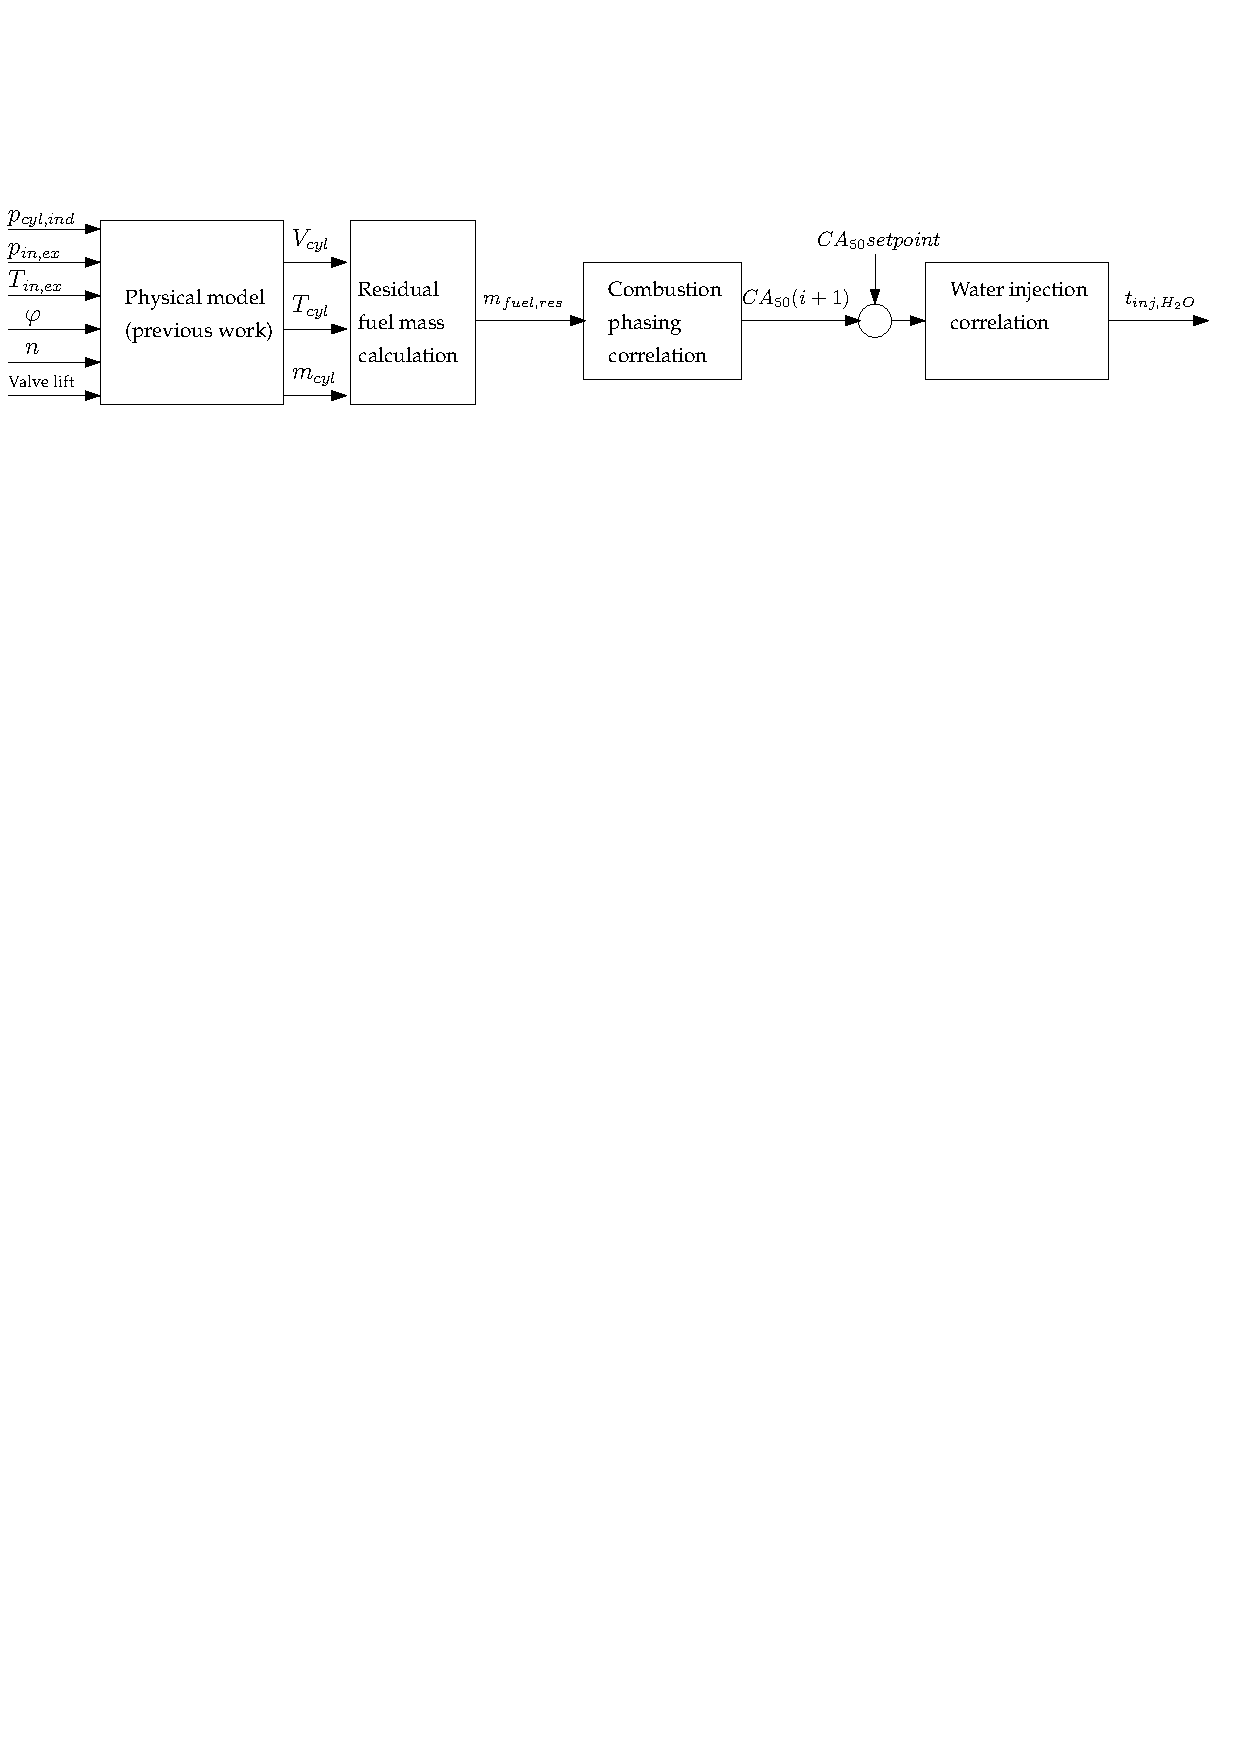
\includegraphics[scale=0.7]{water_ControlModel.pdf}
    \label{fig:ControlModel}
\end{figure}


\end{frame}

%---------------------------------------------------------------SLIDE
\subsection{Fuel mass calculation}
\begin{frame}
\frametitle{Fuel mass calculation}


\begin{equation}
m_{f} = m_{f,inj} - m_{f,b,main} - m_{f,ex} - m_{f,b,NVO}
\end{equation}

\begin{equation}
m_{f,b} = \frac{Q_{b}}{LHV}
\end{equation}

\begin{equation}
m_{f,ex} = \frac{m_{cyl,EVO}-m_{cyl,EVC}}{m_{cyl,EVO}} m_{f,EVO} = x_{ex}\;m_{f,EVO}
\end{equation}

\end{frame}

%---------------------------------------------------------------SLIDE
\subsection{FPGA implmentaion}
\begin{frame}
\frametitle{FPGA - Background}
\begin{columns}
\begin{column}{.4\textwidth}
\begin{block}{Advantages:}
\begin{itemize}
\item Fast sample rate (12.5 ns)
\item Low latency 
\item Parallel computations 
\item Easy of development and update potential compared to application-specific integrated circuits
\end{itemize}
\end{block}\pause

\begin{block}{Challenges:}
\begin{itemize}
\item Individual calculation delay
\item Fixed point arithmetic
\item Limited calculation types
\end{itemize}
\end{block}
\end{column}

\begin{column}{.4\textwidth}
\begin{block}{test}
Test
\end{block}
\end{column}
\end{columns}
\end{frame}


%---------------------------------------------------------------SLIDE
\begin{frame}
\frametitle{FPGA - Timing requirement}

\end{frame}

%---------------------------------------------------------------SLIDE
\begin{frame}
\frametitle{FPGA - Controller implementation}

\end{frame}

%---------------------------------------------------------------SLIDE
\section{Experimental setup - Single cylinder research engine}
\begin{frame}[t]{Experimental setup}
\begin{minipage}[h!]{.45\textwidth}
\begin{table}[htpb]
%\caption{Single cylinder research engine specification}
\label{Tab:SCREparameters}
\begin{center}
\begin{tabular}{p{4.9cm} p{2.0cm}}
\hline
    Parameter           		& Value \\
\hline
    Displacement volume 		& 0.499 L  \\
    Stroke / bore    	        & 90 / 84 mm    \\
    Compression ratio   		& 12:1     \\
    Valve train             	& EMVT   \\
    Max. valve lift (In/Ex) 	& 8 mm/8 mm \\
    Intake / exhaust pressure  	& 1013 mbar \\
    Intake temperature          & 50 $^{\circ}$C \\
    Oil and coolant temperature & 90 $^{\circ}$C \\
    Engine speed                & 1500 rpm \\  
\hline
\end{tabular}
\end{center}
\end{table}
  \end{minipage}\hfill\hfill 
   \begin{minipage}[h!]{.45\textwidth}
      
      \end{minipage}
\end{frame}
%---------------------------------------------------------------SLIDE
\subsection{Combustion phasing correlations}
\begin{frame}
\frametitle{Combustion phasing correlations}
\begin{columns}
\begin{column}{.65\textwidth}
\begin{figure}[htbp]
\centering
    \setlength{\figH}{4cm}
    \setlength{\figW}{7cm}
	% This file was created by matlab2tikz.
%
%The latest updates can be retrieved from
%  http://www.mathworks.com/matlabcentral/fileexchange/22022-matlab2tikz-matlab2tikz
%where you can also make suggestions and rate matlab2tikz.
%
\definecolor{mycolor1}{rgb}{0.8,0.8,0.8}%
%\definecolor{mycolor1}{rgb}{0.00000,0.44700,0.74100}%
\definecolor{mycolor2}{rgb}{0.85000,0.32500,0.09800}%
%\definecolor{mycolor3}{rgb}{0.92900,0.69400,0.12500}%
\definecolor{mycolor3}{rgb}{0,0,0}%
\definecolor{mycolor4}{rgb}{0.49400,0.18400,0.55600}%
\definecolor{mycolor5}{rgb}{0.46600,0.67400,0.18800}%
\definecolor{mycolor6}{rgb}{0.30100,0.74500,0.93300}%
\definecolor{mycolor7}{rgb}{0.63500,0.07800,0.18400}%
\definecolor{mycolorFIT}{rgb}{1,0,0}%
%
\begin{tikzpicture}
\begin{axis}[%
width=0.950\figW,
height=\figH,
at={(0\figW,0\figH)},
scale only axis,
xmin=0,
xmax=12,
xlabel={Residual fuel mass at EVC $m_{f,EVC}$ (i) [mg]},
ymin=-20,
ymax=40,
ytick={-20, -10, 0, 10, 20, 30, 40},
ylabel={$CA_{50}$ (i+1) [$^{\circ}$CA aTDC]},
axis background/.style={fill=white},
legend style={legend cell align=left,align=left,draw=white!15!black},
ticklabel style={font=\footnotesize},axis on top,every axis plot post/.style={line join=round},legend style={cells={anchor=west},draw=none,fill=white,font=\footnotesize,legend pos= north east,legend style={row sep=0.3pt}},/pgf/number format/.cd,1000 sep={},
]
\addplot [color=mycolor1,only marks,mark=*,mark options={solid,fill=white!70!black,draw=white!70!black}]
  table[row sep=crcr]{%
1.358708753	12.4\\
2.235694656	12.4\\
2.77892139	13\\
2.994445549	15.2\\
3.263199913	9.6\\
3.377515521	25.1\\
4.809239365	-2.9\\
4.412591072	2\\
4.297743621	4\\
4.053066942	7.9\\
3.754548037	12.9\\
3.619637737	17\\
3.482293127	14.1\\
3.308193601	25.7\\
4.24095046	1.1\\
4.1931608	4.6\\
4.067899041	12.4\\
3.646340125	16.9\\
3.602028283	9.9\\
3.502131773	13.5\\
3.505638717	11.6\\
3.610567013	14.5\\
3.660387735	11.8\\
3.467966568	16.7\\
3.445776573	11.7\\
3.23052188	11.2\\
3.069486839	14\\
3.131430961	12\\
3.254149552	16.7\\
3.166118361	11\\
3.297806086	14.2\\
3.334858959	17\\
3.287773774	10.1\\
3.202955889	9.5\\
3.271460133	8.6\\
3.465949376	11.1\\
3.467567119	12\\
3.532492318	20.3\\
3.85085521	7\\
3.981493356	9.1\\
3.665371757	10.2\\
3.442099362	12.2\\
3.333788148	10.3\\
3.274201401	18.7\\
3.552630905	10.9\\
3.256316264	12.1\\
3.344962264	14.6\\
3.58594614	14.6\\
3.662717196	12.4\\
3.719671794	19.9\\
4.033012522	8.2\\
3.890876475	11\\
3.753634476	13.5\\
3.563383033	15.3\\
3.362655014	17.1\\
3.322667177	10.6\\
3.344490155	19.5\\
3.677403662	10.1\\
3.710549496	9.7\\
3.476309448	11\\
3.574251229	16.1\\
3.399859801	18.1\\
3.69723741	7.5\\
3.706749385	19.4\\
3.885777653	5.7\\
3.686663543	9.8\\
3.436688966	18.6\\
3.453724068	7.1\\
3.571253379	11\\
3.587578876	16.4\\
3.597584586	11\\
3.482431844	16.7\\
3.68798223	12.2\\
3.580504407	18.3\\
3.84715763	9.4\\
3.851835926	23.4\\
4.298161436	2.1\\
4.125364744	5.2\\
4.195399602	16.5\\
3.801432605	6.7\\
3.695320261	9.5\\
3.678033532	9.6\\
3.55675642	15\\
3.436664464	12.6\\
3.50500024	8.5\\
3.86573631	15.7\\
3.915337692	12.2\\
3.809444052	20.7\\
3.692022441	6.3\\
3.518090979	11.2\\
3.48311496	9.7\\
3.611639983	14.1\\
3.45783753	13\\
3.662797208	16.4\\
3.589579438	13.7\\
3.64011649	12.3\\
3.622292069	19.8\\
3.915979147	8\\
3.86073637	12.2\\
3.765057481	13.8\\
3.575051579	23.2\\
3.942299909	5.5\\
3.929242906	8.7\\
4.171274003	13.4\\
3.849026245	10.8\\
3.804457169	19.6\\
3.880672978	8.7\\
3.870947618	12.7\\
3.708875655	15\\
3.663586481	11.2\\
3.832232938	19.4\\
4.072017504	4.9\\
3.866089674	8.1\\
4.037223929	19.5\\
4.034096251	4.7\\
4.099857043	12.4\\
3.820271129	12.6\\
3.66359409	11.7\\
3.669870759	17.7\\
4.024087349	8.5\\
4.041700345	20.3\\
4.455659028	3.3\\
4.338019922	8.2\\
4.238900346	15.3\\
3.7117269	12.4\\
3.344742113	18.8\\
3.336456667	8.5\\
3.386093142	10.1\\
3.422725835	12.5\\
3.311503167	12.3\\
3.586965913	14.2\\
3.713984846	20.7\\
4.174618386	5.4\\
4.045718148	10.7\\
4.031805763	13.5\\
3.80862119	11.7\\
3.542482963	15.5\\
3.448647717	11.7\\
3.467049065	17.7\\
3.712909386	8.2\\
3.731704034	27\\
4.741531576	-0.7\\
4.798069781	3.3\\
4.444046936	14.8\\
4.082678792	10.7\\
3.852976487	20.5\\
3.932997826	7.5\\
3.968708671	13.5\\
3.816271375	16.9\\
3.639480602	12.4\\
3.533965194	15.4\\
3.466384578	10.5\\
3.30342914	16.4\\
3.297926452	10.9\\
3.276233459	17.7\\
3.25476778	10.3\\
3.543412278	17.3\\
3.67141156	9.9\\
3.587133914	14.4\\
3.557296069	15.2\\
3.560649514	21.6\\
3.618471332	4\\
3.589747327	8.3\\
3.59138786	13.9\\
3.654062912	15.8\\
3.38649027	11.1\\
3.267998675	14.1\\
3.235819948	15.2\\
3.1641562	13.2\\
3.347509101	27.9\\
4.571524902	-1\\
4.219862759	0.8\\
4.195758374	5.6\\
3.778344039	14.2\\
3.565262127	13.9\\
3.47928857	10.4\\
3.538664867	16.1\\
3.477550246	8.6\\
3.638625604	20.1\\
3.842905483	7.2\\
3.809251685	15\\
3.722888983	11.2\\
3.502415406	17.5\\
3.524329693	8\\
3.598536398	11.9\\
3.754660557	13.2\\
3.531664078	12.9\\
3.544545847	14.3\\
3.574062536	13.8\\
3.620411703	16.6\\
3.656217851	10.4\\
3.739018799	12.6\\
3.466568806	12.7\\
3.163981622	14\\
3.097752355	16.7\\
3.245104408	13\\
3.327885079	16.4\\
3.433157143	10.1\\
3.392208415	14.9\\
%\addplot [color=mycolor2,only marks,mark=*,mark %options={solid,fill=white!70!black,draw=white!70!black}]
%  table[row sep=crcr]{%
1.395672421	12\\
2.248512745	29.6\\
4.331602368	-0.7\\
4.30183065	1.5\\
4.318333086	9.3\\
3.96152403	13.6\\
3.606942682	20.6\\
3.602926249	8.1\\
3.684858262	14.9\\
3.621870395	13.6\\
3.400031795	11.1\\
3.36524072	17.6\\
3.524527152	6.5\\
3.498160002	8.3\\
3.294456465	11.1\\
3.322321428	15.7\\
3.474737701	10.2\\
3.483965096	17.1\\
3.510608065	9.4\\
3.419423361	13.2\\
3.316512498	17.8\\
3.384556678	13.9\\
3.269930016	14.1\\
3.269154567	14.9\\
3.349656912	11.5\\
3.42014484	15.8\\
3.324104411	12.1\\
3.177778285	16.1\\
3.014381062	13.5\\
3.021839659	13\\
3.20977348	13.3\\
3.167763256	12\\
3.308716934	12.6\\
3.395914204	15.6\\
3.453177557	15.7\\
3.210642564	8.5\\
3.370252128	14.1\\
3.145814354	15.8\\
3.005562164	11.3\\
3.285430819	22.3\\
4.053522766	0.1\\
4.3025356	-0.1\\
4.240474099	4.2\\
3.983172693	11.4\\
3.650064949	12.7\\
3.434378197	12.1\\
3.414398878	10.4\\
3.290621314	15.8\\
3.423674208	12.6\\
3.131321305	19.9\\
3.295838765	6.6\\
3.49695204	12.3\\
3.448359755	10.1\\
3.408035397	18.9\\
3.466337282	4.4\\
3.577112308	6.6\\
3.582947581	11.1\\
3.321523023	18.9\\
3.401837656	8.4\\
3.478702795	14.5\\
3.403159804	13.4\\
3.151022302	13.6\\
3.182416475	12.6\\
3.247129226	20.9\\
3.415081632	6.1\\
3.59111133	11.8\\
3.577084425	13.4\\
3.37688613	13.3\\
3.467874888	15.8\\
3.49151049	10.6\\
3.448810918	19\\
3.405487435	9\\
3.452083165	13.4\\
3.392615095	9.9\\
3.286082673	14.6\\
3.343331727	11.8\\
3.330651525	13.6\\
3.320633529	12.1\\
3.192745995	15.5\\
3.220747264	11.1\\
3.251709811	15.1\\
3.347082058	15.3\\
3.263321055	12.5\\
3.439997273	16.9\\
3.373364244	8.8\\
3.399255213	17\\
3.482033081	12.6\\
3.340516947	19.8\\
3.575747532	8.8\\
3.459319788	13.3\\
3.550813705	16.4\\
3.395766298	15.4\\
3.376617681	21\\
3.452727039	7.5\\
3.579971238	10.9\\
3.549572748	14.7\\
3.349998255	12.2\\
3.188010138	9.7\\
3.190609257	14.7\\
3.160244653	10.1\\
3.114183321	12.7\\
3.204903532	15.8\\
3.094475481	8.9\\
3.286274513	10.4\\
3.299896377	15\\
3.147007634	10.2\\
3.212549046	14.6\\
3.218732135	14.9\\
3.114969253	15.8\\
3.119137507	14.1\\
3.070113091	6.8\\
3.217206395	11.4\\
3.118421182	10.8\\
3.213311771	13.1\\
3.371623891	13.1\\
3.258661586	19.1\\
3.466033622	7.7\\
3.430381373	14.9\\
3.345350945	13.9\\
3.306816596	17.1\\
3.268934166	10.8\\
3.365570451	22.6\\
3.917564455	4.1\\
3.805387017	6.8\\
3.761620441	12.6\\
3.666916409	11.7\\
3.601711469	16\\
3.565667708	11.3\\
3.600672326	23.4\\
3.922961069	1.6\\
4.075897296	2.4\\
4.133590795	9.4\\
3.61695913	13.8\\
3.219486873	14.9\\
3.278430405	15\\
3.410382153	18.8\\
3.576796618	9.4\\
3.786210451	12.7\\
3.822274319	14.4\\
3.656869682	9\\
3.705059841	16\\
3.679617107	12.3\\
3.593765661	16.6\\
3.49789554	13.4\\
3.392383842	13\\
3.486409102	13.5\\
3.516373304	13.3\\
3.681888596	13.8\\
3.649477227	13.2\\
3.55956344	14.3\\
3.711427572	10.9\\
3.623865792	16\\
3.494686792	18.7\\
3.486555535	9.6\\
3.564960422	10.9\\
3.546398694	16.7\\
3.446607825	9.3\\
3.607725557	9.4\\
3.694340275	14.2\\
3.716647399	13.5\\
3.856828644	23.2\\
4.25682435	4.5\\
4.060942234	6.3\\
3.980635786	12.9\\
3.680821188	16.4\\
3.445944316	10.3\\
3.278059826	18.9\\
3.35200488	8.4\\
3.370659928	11.2\\
3.244794773	12.3\\
3.223070897	12.9\\
3.275262211	10.8\\
3.24915255	15.1\\
3.374913412	13.3\\
3.335607338	11.1\\
3.421997284	12.6\\
3.572956792	14.6\\
3.516340421	15.7\\
3.536185113	15.3\\
3.484723059	11.9\\
3.500104202	11.1\\
3.608836605	27.6\\
5.051776111	-3\\
4.958584737	0.7\\
4.780151031	8\\
3.981715834	10.4\\
3.64075754	14.9\\
3.457697255	12.9\\
3.370520448	12.9\\
3.379450906	16.3\\
3.418971333	9.9\\
3.492556672	16.8\\
3.504953885	8.6\\
3.499082015	24.5\\
4.737179912	-2.8\\
4.561749662	1.4\\
4.539480481	9.1\\
4.04191801	9.8\\
3.667580989	9.4\\
%\addplot [color=mycolor3,only marks,mark=*,mark %options={solid,fill=white!70!black,draw=white!70!black}]
%  table[row sep=crcr]{%
1.259696472	23.8\\
3.315384	-1.1\\
3.545288842	0.4\\
3.789494818	3.6\\
3.61935511	9.9\\
3.5234916	17.6\\
3.634439332	11.4\\
3.592992725	24.5\\
4.788061924	0.2\\
4.599652641	4\\
4.433478854	13.6\\
4.137098319	13.1\\
3.9831834	19.7\\
3.912807776	8.4\\
3.992100636	16.9\\
3.740598558	14.3\\
3.475603274	18.2\\
3.529682607	12.3\\
3.387142622	11.3\\
3.684904833	14.5\\
3.727938028	10.7\\
3.848597754	25.6\\
6.927426005	-9.3\\
5.174325493	-0.6\\
5.212132691	1.9\\
4.576318901	13.1\\
4.048100473	7.7\\
3.775804352	13.6\\
3.736489442	15.7\\
3.834100373	15.9\\
3.918333864	13.2\\
3.892855745	17.4\\
4.091801496	10.6\\
4.140574848	22.7\\
4.463477412	5.5\\
4.355806933	11.3\\
4.269321082	12.4\\
4.02594207	16.3\\
4.034710765	13.5\\
4.129131302	14.2\\
3.811730438	10.9\\
3.855440489	13\\
3.728903098	11.9\\
3.874235651	22.7\\
4.441567133	5.2\\
4.233449502	9.4\\
3.976753317	15.4\\
3.88589181	11.5\\
3.918457607	15.9\\
3.929293235	11.4\\
3.908697118	27.5\\
6.191503533	-3.4\\
5.459339985	0.5\\
5.012890954	9.5\\
4.607838692	12.8\\
4.269771116	14.7\\
3.978832543	14\\
3.823378139	13.8\\
3.798446126	16.1\\
3.684699379	13\\
3.641662021	15.4\\
3.697281631	8.7\\
3.677706434	13.5\\
3.48527412	12.3\\
3.81475735	19.3\\
3.753763923	9.7\\
3.799177	14.9\\
3.760013349	17.1\\
3.593507397	10.9\\
3.700228142	31.7\\
7.073121644	-6.3\\
5.729209103	-1.6\\
5.219743744	4.2\\
4.877244436	10\\
4.360962868	11.9\\
4.281017915	14.4\\
3.979080811	16.3\\
3.888100108	19\\
3.830293885	9.2\\
3.904432834	15.2\\
3.776775249	14.5\\
3.809103923	9.2\\
3.899905095	19.8\\
4.429046835	3.3\\
4.441100707	8.6\\
4.084429829	18.2\\
3.875455103	9.9\\
3.700019713	17.4\\
3.761791515	8.9\\
3.713335652	22.2\\
3.886524691	4.3\\
3.860208651	9\\
3.84160504	21.1\\
4.522199309	3.9\\
4.443244116	9.5\\
4.179252417	15.8\\
3.983053496	11\\
3.857771323	30.3\\
7.746427949	-10\\
5.740572877	0.4\\
5.232403801	3\\
4.548429018	11.2\\
4.274799716	26.4\\
4.927368801	-2.2\\
4.949803365	4.7\\
4.62816749	10.3\\
4.225630538	15.8\\
4.007574546	14.4\\
3.865104602	12.5\\
3.748291388	13\\
3.837476104	14.4\\
3.830074364	17.2\\
3.760922327	11.3\\
3.596274306	15.1\\
3.580719884	15.4\\
3.677323094	12.5\\
3.865924773	21.7\\
3.803172675	6.4\\
3.800072649	9.7\\
4.027807364	18.5\\
4.122828477	6.9\\
4.178185155	19\\
4.373335917	6.8\\
4.144687737	22.4\\
4.562088032	5.6\\
4.255981582	10.6\\
4.06442865	11.3\\
3.993297911	34\\
7.548167446	-9.2\\
6.131084038	0.8\\
5.213033296	6.1\\
4.548264447	13.6\\
4.327449771	12.9\\
4.306322941	23.7\\
5.363035358	-2.4\\
4.62825228	5\\
4.453141862	13.8\\
3.996628927	10\\
3.735270586	13.5\\
3.750218502	14.4\\
3.836750389	19\\
3.975982145	10.5\\
3.999529163	23.3\\
4.528020848	4.7\\
4.690211597	15.5\\
4.488384235	12\\
4.169233964	17.7\\
4.147934596	11.4\\
4.15080196	19.6\\
4.123540186	8.8\\
4.252618858	11.6\\
4.249809399	17.9\\
4.010421143	10.6\\
3.849261906	17.7\\
4.167379873	10.5\\
3.907125614	20.3\\
4.326564254	5.7\\
3.945437478	8.1\\
3.744201502	19.7\\
3.80075604	6.7\\
3.745204237	16.8\\
3.730573925	15.3\\
3.668405986	20\\
3.945079579	8.6\\
3.824829547	20.9\\
3.947628616	6.9\\
3.793079083	14.5\\
3.597528198	12.8\\
3.684788084	24\\
5.151911363	-2.1\\
4.606412052	1.4\\
4.407797701	7\\
4.184380616	14.7\\
4.098713445	16.2\\
3.847375322	17.4\\
3.803551219	11.9\\
3.856662687	24.8\\
4.364764706	4.8\\
4.185282273	8.8\\
4.014066767	19.7\\
4.111284448	8.9\\
3.935733669	22.3\\
4.981260105	1.2\\
4.355795018	4.7\\
4.101881243	9.3\\
3.836489989	13.6\\
3.472491268	11.7\\
3.261673198	20.5\\
3.612874722	4.6\\
3.665199649	17.3\\
3.757806443	10.7\\
3.915054323	18.5\\
3.986543923	14.9\\
3.726137228	18.1\\
3.860456755	11.8\\
3.820071975	25.7\\
4.284866491	3.9\\
4.224746791	9.5\\
4.149237145	12.2\\
%\addplot [color=mycolor4,only marks,mark=*,mark %options={solid,fill=white!70!black,draw=white!70!black},forget %plot]
%  table[row sep=crcr]{%
2.22144621	0.1\\
3.126903075	4.2\\
3.363993753	14.1\\
3.38323348	19.5\\
3.466842916	9.6\\
3.619216414	18.9\\
3.758801357	11.4\\
3.767311244	24.6\\
4.454291932	2\\
4.376638228	5\\
4.04468594	9\\
3.69192382	15\\
3.657069874	24.2\\
4.006757474	6.3\\
4.072526703	11.8\\
4.03733501	25.2\\
5.622853465	-4\\
4.926843711	0\\
4.893726094	2.8\\
4.281781411	8.5\\
4.012000459	20.3\\
3.916488174	8.5\\
3.758437598	19.9\\
3.755298621	8.5\\
3.79558254	27.7\\
4.990036786	-1.2\\
4.771139788	1.8\\
4.566537209	7.5\\
4.265363808	22\\
4.363979931	4.1\\
4.294315544	18\\
3.94521051	13.4\\
3.744112011	18.2\\
3.576497141	13.7\\
3.58349204	22.2\\
4.22221048	3.3\\
4.213279937	11.4\\
4.085016071	23.9\\
4.618194946	2.4\\
4.690557379	7.7\\
4.435020195	21.7\\
4.619315828	4.7\\
4.223616307	10.4\\
3.956876777	26.2\\
5.219129526	-4.2\\
4.674440799	2\\
4.752163354	7.4\\
4.243815807	21.6\\
4.643155314	1\\
4.492333883	5.4\\
4.263568013	16.2\\
3.855008752	12.4\\
3.653034302	16.5\\
3.664626065	11.9\\
3.603422993	16.1\\
3.531821711	12.8\\
3.637610056	23.5\\
4.868964648	1.1\\
4.808371056	4.3\\
4.668783529	12.2\\
4.021748841	16.4\\
3.756871309	10.4\\
3.588192281	20.3\\
3.85583293	6.3\\
3.84137121	10.9\\
3.714399447	16.3\\
3.741637667	11.3\\
3.585374533	11.7\\
3.4577616	17\\
3.477828836	9.4\\
3.409573361	19.1\\
3.354128471	9.1\\
3.398574889	17.2\\
3.487833338	12.3\\
3.424184808	35.1\\
6.271053366	-6\\
5.511412481	0.3\\
5.053666192	4.8\\
4.195216548	10.8\\
3.608986192	20.1\\
3.645890151	12.1\\
3.642379571	28\\
4.477863408	-0.9\\
4.411907437	3.5\\
4.220613944	7.5\\
3.888105741	12.5\\
3.673048396	17.2\\
3.845033202	17.2\\
3.641770733	26.6\\
4.484586494	2.3\\
4.397636478	4.5\\
4.248446024	10.5\\
4.014341369	13.2\\
3.921711942	17.5\\
3.911942111	19.4\\
3.784077295	8.3\\
3.926707782	16.9\\
3.946969506	11.4\\
3.876705615	30.7\\
10.02879692	-14.3\\
6.732653773	9.9\\
5.436450306	11.3\\
4.356241492	20.7\\
4.229179867	10\\
3.978443171	12.3\\
3.630768103	15.3\\
3.536815622	19.1\\
3.590485972	9.9\\
3.603267385	12.9\\
3.547644005	13.7\\
3.667766587	15.2\\
3.770068132	13.1\\
3.635654966	13\\
3.560736852	16.8\\
3.492681087	11\\
3.5387366	27.1\\
8.413392341	-11.4\\
6.490811458	6.9\\
5.093184621	5.6\\
4.608804396	13.2\\
4.238422624	17.5\\
4.098291575	11.5\\
4.026848305	19.3\\
4.170525048	6.8\\
4.018424553	15.8\\
3.891877685	14.8\\
3.648106171	15.5\\
3.665697555	13.5\\
3.71775501	17.1\\
3.926753163	7.8\\
3.919606587	24.6\\
5.231648131	-4.6\\
4.631072352	0.6\\
4.488006558	8.7\\
4.188211777	14\\
3.947431929	14.9\\
3.845253319	21.7\\
3.935785397	6.1\\
3.963008255	9.9\\
3.70272385	17.5\\
3.623637216	11.8\\
3.52586462	15.6\\
3.421871882	17.9\\
3.268400792	15.8\\
3.321312318	14.9\\
3.242843591	20.8\\
3.612277388	6.5\\
3.804590929	10\\
3.566656753	18.3\\
3.455632505	10.4\\
3.612066635	21.2\\
3.946456885	5\\
3.87704208	14.4\\
3.752352569	13\\
3.804342723	20.5\\
3.851267093	9.7\\
3.824367823	18.6\\
4.070718731	10\\
3.972387164	20\\
4.439635416	5.2\\
3.854978464	9.5\\
3.681695845	17.5\\
3.437885734	10.7\\
3.314569694	13.7\\
3.276508983	19.9\\
3.382991151	8.8\\
3.345198173	19.4\\
3.419309266	7.8\\
3.38006337	12.9\\
3.286887693	15.5\\
3.349275792	12\\
3.252102649	17.9\\
3.336791521	8.8\\
3.392379044	14.6\\
3.227600684	25.8\\
3.997250599	1.9\\
4.273921433	3.2\\
4.23266103	16.7\\
3.984856761	11.9\\
3.857802651	17.6\\
3.765412164	9.4\\
3.480462548	20.4\\
3.811964125	5.6\\
3.744284997	9.3\\
3.59872631	22.1\\
3.973998957	4.3\\
3.923013489	5.9\\
3.740696602	14.8\\
3.598525515	12.4\\
3.37310605	21.3\\
3.706160092	5.1\\
3.652688146	15.5\\
3.431646323	14.6\\
3.291490762	18.3\\
3.489799338	13\\
3.327002256	32.1\\
5.985194261	-7.3\\
5.409425019	-0.9\\
4.938553728	6.1\\
%\addplot [color=mycolor5,only marks,mark=*,mark %options={solid,fill=white!70!black,draw=white!70!black},forget %plot]
%  table[row sep=crcr]{%
1.097866804	9.6\\
2.077278841	22.1\\
2.95142344	5.9\\
3.292772432	9.4\\
3.486102767	12.3\\
3.490447959	11.5\\
3.495336084	15.8\\
3.427669333	15.6\\
3.331245249	12.1\\
3.347030336	17.5\\
3.320461267	8.4\\
3.367549285	7.9\\
3.437361205	15.1\\
3.455100794	15.5\\
3.420684327	15.2\\
3.551452249	13.1\\
3.502782348	15.4\\
3.476081565	13.5\\
3.54199029	14.5\\
3.491445374	11.4\\
3.71541106	13\\
3.625591679	16.3\\
3.526804821	14.1\\
3.695454368	12\\
3.719486803	30.9\\
6.059661499	-6.3\\
5.257969587	-0.5\\
4.770356046	4.7\\
4.243060782	11.4\\
3.831775206	14.8\\
3.370317503	14.9\\
3.448683051	24.1\\
3.847888697	4.9\\
3.941172631	11\\
3.722839736	18.4\\
3.603490773	10\\
3.613452761	22.9\\
4.10756093	2.3\\
3.964517641	8.3\\
3.931369854	15\\
3.708549173	15.1\\
3.546385669	24.8\\
4.093894455	4\\
4.27317367	11\\
3.989871089	15\\
3.744754997	18.2\\
3.725526257	9.3\\
3.541110531	15.5\\
3.559506921	19.6\\
3.841132886	9.3\\
3.841088618	14.5\\
3.825402897	15.4\\
3.602469094	20.1\\
3.503119842	11.9\\
3.434145829	16.4\\
3.286452692	12.3\\
3.43344722	20\\
3.654333624	7.1\\
3.654232857	12.8\\
3.680918126	16.3\\
3.762433268	14.7\\
3.797366301	24.2\\
4.008514662	4.2\\
4.102819658	6.8\\
3.995452316	13.2\\
3.677136775	14.9\\
3.633285676	13.7\\
3.601927681	15.8\\
3.715807856	17\\
3.762658781	11\\
3.812918552	17.8\\
3.774929558	8.5\\
3.802466828	16.7\\
3.668480398	12.2\\
3.704729752	27.4\\
5.719545348	-4.4\\
4.971569203	-0.7\\
4.816080421	1.7\\
4.369318924	8.2\\
3.927904629	16.4\\
3.704566533	14\\
3.481218154	14.1\\
3.620038626	17.2\\
3.687148381	12.9\\
3.622824057	28.6\\
4.860236418	-1.9\\
4.624541199	1.2\\
4.70306634	6.6\\
4.322250716	12.9\\
3.906113615	14.9\\
3.83801656	18.1\\
3.695126613	11.9\\
3.525882563	19.2\\
3.556201083	5.7\\
3.723894109	10.4\\
3.610820272	13.7\\
3.577894386	16.1\\
3.637931981	14\\
3.670992626	20.6\\
3.822425185	8.4\\
3.927630765	11.7\\
3.741360252	16\\
3.661257467	14.3\\
3.622129589	25.8\\
4.483553677	1.5\\
4.459485705	6.7\\
4.233692905	13\\
3.983849884	20.1\\
4.091584992	8.2\\
4.057650979	13.8\\
3.809194598	15.2\\
3.662594457	23\\
4.131799813	4.7\\
3.948404753	7.7\\
3.972253923	13.3\\
3.807582532	11.3\\
3.767194601	17.7\\
3.705125137	11.3\\
3.611390199	24.9\\
4.757647144	-0.4\\
4.71479282	1\\
4.67275756	6.8\\
4.236069898	12.2\\
3.924096436	22.2\\
4.146253558	3.1\\
4.065548646	8.3\\
3.876325769	18.7\\
3.685395786	8.8\\
3.780238411	23.8\\
4.524464615	1.4\\
4.325626365	6\\
4.177353571	15.1\\
3.593709387	16.6\\
3.511071563	12\\
3.532897779	12.5\\
3.415640694	19.3\\
3.452336553	10.2\\
3.509160233	25.2\\
4.337550631	-1.1\\
4.406123468	3.2\\
4.370055218	9.3\\
3.902703679	12.9\\
3.862927408	26.3\\
4.715093286	2.7\\
4.358325953	12.3\\
3.951764233	15\\
3.85241499	18.2\\
3.671877673	10.7\\
3.707660739	17.6\\
3.423062973	10.1\\
3.449953012	13\\
3.526616351	10.9\\
3.448253523	12\\
3.419062311	17.7\\
3.399030598	10.8\\
3.586585064	22.3\\
4.271693708	4.7\\
4.011170883	14.2\\
3.724561895	14.5\\
3.542093537	18.6\\
3.782918352	9\\
3.718074049	15.6\\
3.521764486	12.8\\
3.344824429	11.9\\
3.40634954	15.4\\
3.412010465	24.6\\
4.508613758	0.9\\
4.344228634	2.1\\
4.150783433	9.6\\
3.722583005	13.8\\
3.463923372	15.5\\
3.437658885	20.8\\
3.509148404	9.9\\
3.483437224	15.4\\
3.523139309	16\\
3.539810202	16.7\\
3.487106079	31.6\\
5.384635449	-2.4\\
5.090187882	-0.8\\
4.889835367	5.9\\
4.415662762	15\\
4.023860488	13.7\\
3.820376416	19.4\\
3.930804572	6\\
3.744310994	12.7\\
3.438472693	15.4\\
3.462513874	13.8\\
3.646640924	19.2\\
4.007051143	7.8\\
3.962634062	20.4\\
3.875268889	9\\
3.662882681	15.9\\
3.534476423	16.5\\
3.361747768	22.3\\
3.563919753	4.8\\
3.497084507	7.2\\
3.577006617	16.7\\
3.733973574	13.2\\
3.563942259	16.7\\
%\addplot [color=mycolor6,only marks,mark=*,mark %options={solid,fill=white!70!black,draw=white!70!black},forget %plot]
%  table[row sep=crcr]{%
1.605995993	10.6\\
2.402918356	7.8\\
2.968550897	11.8\\
3.130206424	7.5\\
3.289386725	11.5\\
3.464933986	8.4\\
3.513769071	12.3\\
3.695783992	16.6\\
3.712151443	8.3\\
3.786635322	8.1\\
3.66953218	20.9\\
3.95926019	-0.2\\
4.137746604	6.2\\
4.192282355	7.5\\
3.89816183	14\\
3.792439794	10.9\\
3.586739829	6.9\\
3.587656885	18.9\\
11.13122634	-0.8\\
4.991794725	-7\\
5.011107098	-1.3\\
4.676052905	3.1\\
4.385157901	7.5\\
4.288588886	6.7\\
3.957829305	6.9\\
3.902417781	14.3\\
3.829969421	10.1\\
3.733703431	10.1\\
3.655843599	16.9\\
3.655177736	8.2\\
3.593780226	6.4\\
3.70508508	26.8\\
5.341743804	-3.9\\
5.091112151	-0.5\\
5.099688832	4.5\\
4.402148459	4.5\\
3.943301844	9.2\\
3.727933655	7\\
3.672582363	21.1\\
3.973377285	1.4\\
4.456331231	9.5\\
4.150196417	8.8\\
3.967755969	15.3\\
3.825758333	4.3\\
3.740941613	18.9\\
3.814325512	5.9\\
3.822042258	12\\
3.593510536	19.6\\
3.556641048	2.1\\
3.806255332	2.8\\
4.066149452	16\\
3.601029627	7.1\\
3.585997146	10.1\\
3.397426396	7.8\\
3.508288861	10.9\\
3.367426457	10.6\\
3.387344566	8.2\\
3.240264202	9\\
3.454568976	9.9\\
3.618345325	10.9\\
3.538041383	3.7\\
3.669355584	9.8\\
3.728338807	10.9\\
3.477653853	7.5\\
3.622223823	9.6\\
3.580957106	9.7\\
3.644635699	10\\
3.629034998	8.9\\
3.676617511	28.3\\
10.282477	-14.3\\
6.488518076	-2.7\\
5.226600749	1.2\\
4.445765255	4.7\\
4.066627648	10.2\\
3.664662353	10\\
3.504195209	4.7\\
3.517730648	23.9\\
9.685319111	-15.5\\
6.636177501	23.2\\
4.990753278	3.9\\
4.5953725	9.5\\
4.044978172	12.2\\
3.509189072	16.9\\
3.569732756	14.4\\
3.599429068	19.4\\
3.713249385	10.7\\
3.499676581	14.4\\
3.40124646	15.5\\
3.339909503	15.1\\
3.234907155	18.8\\
3.659011341	12.7\\
3.49488819	30.9\\
6.54318095	-7.3\\
5.187677832	-0.8\\
5.036504916	2.3\\
4.254246925	11.1\\
3.83955409	17.3\\
3.658841956	11.8\\
3.566869468	23\\
4.569294717	2.4\\
4.095213532	8.4\\
3.71106558	13.3\\
3.442193156	11.1\\
3.560183288	27\\
5.611979202	-6.5\\
5.246113287	-0.6\\
4.977337477	6\\
4.561404141	17.6\\
4.177286655	9.9\\
3.932789491	31.1\\
5.928056684	-5.8\\
4.954910889	-0.4\\
4.725666625	4.3\\
4.359117155	16\\
4.062875267	12.7\\
3.829626772	27.2\\
5.499143592	-1.2\\
5.366396182	4.6\\
4.78137798	14.1\\
4.134884362	10.9\\
3.849594558	15.7\\
3.755900689	14.2\\
3.703340109	13.5\\
3.595791006	22.2\\
4.355717748	3.8\\
4.269732424	11.9\\
4.12626192	19.8\\
4.128241653	7.7\\
4.067628549	29.5\\
6.108019639	-2.7\\
5.496855624	0.3\\
5.229505223	6.6\\
4.590062019	19.4\\
4.189704173	9.6\\
3.825564899	20.1\\
3.727034147	7.5\\
3.686160497	14\\
3.589520324	13.2\\
3.5252722	22.8\\
4.436364396	3\\
4.276045133	8.4\\
4.172294834	27.2\\
6.60125436	-5.1\\
5.551231358	1.2\\
5.200542094	9\\
4.283667661	10.7\\
3.869727335	18.6\\
3.803405722	11.7\\
3.644705323	16.4\\
3.591187699	11.9\\
3.665522682	25.6\\
5.03325142	-2\\
4.726542286	2.8\\
4.779792293	9.3\\
4.361170056	25\\
5.455360115	-1.3\\
5.312553606	3.5\\
4.801258857	14.2\\
4.323115996	13.9\\
3.917675186	21.4\\
4.309923506	4.7\\
4.331082037	24.1\\
4.891486142	0.9\\
4.55040555	9.4\\
4.385549404	11.5\\
3.771896939	16.3\\
3.798255397	18.9\\
3.825838901	12.7\\
3.845449903	18.4\\
4.00997166	12.9\\
3.718080675	20\\
4.065417645	7.4\\
3.871045122	14.4\\
3.683826457	16.7\\
3.829546274	11.9\\
3.527396578	22.5\\
3.803418363	4.9\\
3.81573209	12.6\\
3.332294662	13.6\\
3.44761353	16.2\\
3.357850719	17.4\\
3.342958213	18.1\\
3.24232185	18\\
3.455462433	15\\
3.488785084	14.5\\
3.491107007	24.2\\
3.657374618	5.4\\
3.806558019	15.6\\
3.718776701	14.7\\
3.631382963	27.5\\
5.15564046	-2\\
4.767388658	4.9\\
4.404324088	12\\
4.072525396	19.4\\
4.242146002	10.1\\
3.770450915	15.6\\
3.708511863	14.2\\
3.614434709	19.1\\
3.639292997	8.8\\
%\addplot [color=mycolor7,only marks,mark=*,mark %options={solid,fill=white!70!black,draw=white!70!black},forget %plot]
%  table[row sep=crcr]{%
1.380094058	8.7\\
2.672881068	11.5\\
3.128415703	9.5\\
3.315571578	11.5\\
3.452597092	9.6\\
3.498740827	10.2\\
3.324272351	4.3\\
3.694756408	9.8\\
3.495919114	8.1\\
3.493320001	6.1\\
3.712127305	6.7\\
3.758617262	7.2\\
3.686721892	7.2\\
3.835452407	12.3\\
3.695674976	9.5\\
3.594999775	9.6\\
3.49231358	7.5\\
3.559005414	8.8\\
3.607589574	5.9\\
3.517819496	9.4\\
3.3932363	8.8\\
3.570027074	8.5\\
3.670836087	8.1\\
3.808384313	9.5\\
3.890911823	5.3\\
3.965166669	23.2\\
4.1031599	5.2\\
3.972308061	13.3\\
3.866083523	15.5\\
3.760988097	14.4\\
3.533230839	26.4\\
4.184968149	1.5\\
4.018192565	3.4\\
3.875527777	12.6\\
3.543150219	15.7\\
3.338180551	10.5\\
3.143847031	8.4\\
3.281188856	16.2\\
3.33527514	11.3\\
3.456196017	16.2\\
3.458191737	14.6\\
3.436898915	24.9\\
4.046210091	4.6\\
3.932950968	8.7\\
3.756389694	19.4\\
3.594047227	10.7\\
3.305368915	14\\
3.102370385	14.4\\
2.99609073	18.4\\
3.104692451	8.1\\
3.284254347	17.6\\
3.291593373	11.5\\
3.208721715	18\\
3.407303845	9.1\\
3.435142702	16.3\\
3.396972987	12.1\\
3.392881347	12.2\\
3.377493208	19.5\\
3.338968275	9.6\\
3.297246639	19.4\\
3.369701598	10\\
3.432134482	18.2\\
3.418939531	10.4\\
3.449658977	23.4\\
4.103013941	1.7\\
4.01997924	5.9\\
3.912243356	9\\
3.624044165	23.2\\
3.885350741	5.6\\
3.782148551	12.1\\
3.649310832	11.5\\
3.510156249	13.5\\
3.312068245	12.4\\
3.199986872	19.4\\
3.097284777	9.4\\
3.235983734	23.3\\
3.954100361	3.7\\
4.009276182	8.9\\
3.914113072	14.3\\
3.630744129	18.8\\
3.44915094	9\\
3.380720231	14.1\\
3.131149482	10.7\\
3.110179872	23.3\\
3.638373536	4.1\\
3.662927595	9.6\\
3.641338976	15.9\\
3.523298321	17.1\\
3.450536985	15.7\\
3.318760093	18.7\\
3.326773093	10.6\\
3.315393491	16.6\\
3.303844263	10.3\\
3.331424269	18.1\\
3.502242555	11.1\\
3.266449663	17.9\\
3.396931125	12.5\\
3.311905219	16.6\\
3.382388075	18.1\\
3.428370365	10.6\\
3.387834537	16.2\\
3.314134561	13.3\\
3.325810905	22.8\\
4.073310995	3.5\\
3.972579128	9.6\\
3.77314715	16\\
3.636235717	16.3\\
3.530059584	16.8\\
3.370906287	14.2\\
3.521508535	15.1\\
3.433509162	15.2\\
3.479620949	16.7\\
3.505581832	15.7\\
3.425674889	13.7\\
3.593490944	19.6\\
3.679669471	10.1\\
3.573913337	12.2\\
3.574873716	15.5\\
3.617755956	26.2\\
4.931668308	-0.7\\
4.770385242	-0.6\\
4.348061851	5.5\\
4.047089089	15.9\\
3.613480346	10.7\\
3.521304765	16.2\\
3.473447365	13\\
3.483008298	20.2\\
3.736770207	9.4\\
3.716153422	24\\
4.122072369	3.5\\
4.014323788	15.8\\
3.776161614	13.8\\
3.403169528	27.3\\
4.63553046	-0.9\\
4.200139777	0.7\\
4.385275859	5.8\\
3.960397308	12\\
3.721515568	18.7\\
3.681122872	8.4\\
3.646861262	15.5\\
3.56963873	14.8\\
3.424503542	22.1\\
3.689502116	8.3\\
3.592115252	10.2\\
3.656221521	26.1\\
4.501290685	1\\
4.426591122	5.3\\
4.215041348	13.7\\
3.582940241	15.3\\
3.377459009	15.1\\
3.316679662	19.1\\
3.30294485	11.2\\
3.323105304	13.9\\
3.426559661	22.3\\
3.835171771	6.7\\
3.74495038	16\\
3.640678189	13.6\\
3.458335879	17.7\\
3.473575109	17.3\\
3.253092431	16.3\\
3.14576785	20.5\\
3.331686004	12.5\\
3.345039697	13.7\\
3.343827959	19.9\\
3.497630297	9.1\\
3.457077533	11.5\\
3.488264488	15.2\\
3.375372962	15.3\\
3.280856894	19\\
3.293393679	14.4\\
3.000428698	20.7\\
3.080950092	10.8\\
3.22493814	25\\
4.083288448	0.7\\
3.986994441	4.9\\
4.06340868	12.6\\
3.794763024	16.2\\
3.600607814	12.3\\
3.501057559	18.5\\
3.511384712	11.4\\
3.146657087	19.6\\
3.187682351	9.8\\
3.136568143	15.6\\
3.085671501	14\\
3.131130693	15\\
3.287951923	17.5\\
3.224962336	16.7\\
3.091635836	17.3\\
3.309354363	16.6\\
3.270775554	14.3\\
3.271759808	20.5\\
3.461710865	8.7\\
3.498392697	16.3\\
3.303570008	15.8\\
3.073530226	12.7\\
3.021800506	17.6\\
3.047149026	10.4\\
3.005104902	15.4\\
3.110336368	18.5\\
%\addplot [color=mycolor1,only marks,mark=*,mark %options={solid,fill=white!70!black,draw=white!70!black},forget %plot]
%  table[row sep=crcr]{%
0.8507505544	12.7\\
1.718029096	25\\
3.07554041	1.3\\
3.2600985	4\\
3.462030653	11.7\\
3.16802619	21.1\\
3.77611781	2\\
3.60621909	6.8\\
3.424326305	12.8\\
3.266104269	20\\
3.261991917	7.6\\
3.046121784	15.7\\
3.019940612	13.1\\
3.010135153	13.6\\
2.785262419	15.5\\
2.878191692	11.4\\
2.960169989	16.3\\
2.922373824	13.3\\
2.965984011	18\\
2.869799417	11.8\\
2.814478814	23\\
3.590483643	4.5\\
3.391386997	9.6\\
3.184801463	12\\
2.853269044	20.5\\
2.687778448	8.1\\
2.537704821	9.6\\
2.577721821	10.3\\
2.688584873	32.1\\
4.619975537	-3.9\\
4.166700008	0.9\\
4.259304597	7\\
3.473740884	12.2\\
3.167655059	16.5\\
3.107377561	13.7\\
3.019434185	17.4\\
2.900755625	11.4\\
2.868590366	26.9\\
3.712199842	3.6\\
3.523120927	8.1\\
3.38837029	18.4\\
3.283645407	7.5\\
3.257864088	17.6\\
3.116478297	8.4\\
3.144063334	22.7\\
3.82460706	0.9\\
3.530468689	6.5\\
3.344874627	16.2\\
3.050970769	7.2\\
3.023356489	16.1\\
3.056329003	10.8\\
3.053987644	17.9\\
3.20702533	7.9\\
3.15425472	17.7\\
3.190541793	9.4\\
3.156237745	15.7\\
3.26993287	13.4\\
3.175284289	30.2\\
4.632465158	-1.7\\
4.223335606	3.8\\
4.033229748	11.3\\
3.316428662	16.6\\
3.025060169	9.8\\
2.934800022	18\\
3.174849198	8.3\\
3.274813365	15.3\\
3.092683281	12\\
3.025663983	21.3\\
3.679109362	3.4\\
3.614760357	7.9\\
3.378917689	24.8\\
4.142551034	-1.6\\
4.073770722	2.6\\
3.777750251	11.4\\
3.242374657	10.2\\
3.189474931	15.5\\
3.097187775	18.7\\
3.11542271	9.2\\
3.014464352	17.5\\
3.024023873	9.9\\
2.934047855	15.7\\
3.01838126	16.9\\
3.039373956	10.5\\
3.084324301	15.3\\
3.058032122	13.1\\
2.992696451	19\\
3.226406968	8.4\\
3.092775523	10.7\\
3.020911256	13.3\\
3.022819385	15.4\\
3.039098231	11.1\\
3.098767817	29.8\\
5.375678189	-5.9\\
4.623561043	2\\
4.188206728	7.2\\
3.49735203	10.8\\
3.11676634	9.6\\
3.106214932	19.3\\
3.235364232	8.6\\
3.225096367	15.1\\
3.316055744	14.2\\
3.097926201	15.5\\
3.123462247	11.9\\
3.128906552	33.9\\
6.279857358	-7.7\\
4.621830651	-0.9\\
4.66046699	3.9\\
3.795782774	11.6\\
3.338072063	12.4\\
2.981464704	17.5\\
2.793887359	9.2\\
2.89463963	32.2\\
5.147315074	-4.4\\
4.627739965	-2.3\\
4.482093144	4.2\\
3.93335799	8.3\\
3.414284604	12.9\\
3.211489279	13.6\\
3.020206034	15\\
3.097991765	16.1\\
2.983376998	14.5\\
2.749369405	14.2\\
2.687754689	18.3\\
2.642473705	12.7\\
2.573775731	14.6\\
2.697820512	10.6\\
2.823595989	19.6\\
3.043868187	9.4\\
3.096803842	31.2\\
5.131641152	-5.8\\
4.262820478	-1.4\\
4.212332203	4.7\\
3.63456981	15.8\\
3.225708577	7.7\\
3.050449297	16.6\\
2.875448708	15\\
2.797035935	15.3\\
2.812803604	22.8\\
3.231430515	4.4\\
3.145807427	10.5\\
2.985663902	10.2\\
2.783858804	11\\
2.751909009	17.2\\
2.683118987	11.1\\
2.587719932	18.6\\
2.851932908	9.2\\
2.897147109	21\\
3.361823917	5.5\\
3.256509737	11.9\\
3.140872703	13.6\\
2.950602087	17.5\\
2.843540959	10.8\\
2.781185246	17.4\\
2.789163265	12.3\\
2.581496249	14.1\\
2.576564972	13.9\\
2.705479733	27.8\\
4.404655896	-0.2\\
3.897133641	4\\
3.615209778	7.9\\
3.236430824	17.4\\
3.178701438	10.6\\
2.750654205	18.8\\
2.907608796	7.3\\
2.867665764	24.6\\
3.88547805	-1.3\\
3.478490951	1.7\\
3.529856853	8.7\\
3.08502347	9.9\\
2.971340715	16.4\\
3.020745547	12.6\\
2.941273618	13.2\\
2.952612798	21.1\\
3.157206795	7.3\\
2.887672351	18.2\\
2.834497186	9.6\\
2.606851334	16.3\\
2.608438343	10\\
2.810361323	10.3\\
2.734899961	15.2\\
2.675536593	10.9\\
2.622680574	23.7\\
2.981950241	4.5\\
2.950766179	7.4\\
3.034758621	12.8\\
2.787140769	16.4\\
2.767241743	12.6\\
2.743879884	24.7\\
3.341791408	0.2\\
3.394457873	5\\
3.309322477	13\\
2.932204379	13.7\\
2.742958852	17.9\\
2.814516984	11.1\\
2.76936301	13.2\\
2.845989004	14.6\\
2.89172591	19.3\\
3.028464182	11.5\\
2.878530131	19\\
%\addplot [color=mycolor2,only marks,mark=*,mark %options={solid,fill=white!70!black,draw=white!70!black},forget %plot]
%  table[row sep=crcr]{%
1.186106969	17.7\\
2.382527068	7.1\\
2.751452784	17.7\\
3.123652346	6.8\\
3.147025335	10.4\\
3.049731191	10.7\\
3.18345337	14.1\\
3.25386902	16.2\\
3.275010097	8.5\\
3.149285741	6.2\\
3.344775586	7.2\\
3.390951694	9.4\\
3.400743734	10.6\\
3.205551938	11.8\\
3.210280016	22.4\\
3.715698122	-0.2\\
3.462169561	3.5\\
3.488741554	10.9\\
3.160723614	6.9\\
3.222809089	20.2\\
3.44035424	4.6\\
3.730795506	8.2\\
3.571476946	13.9\\
3.406683242	10.3\\
3.345069619	9.4\\
3.347834242	8.4\\
3.394800266	8.9\\
3.311296015	8.4\\
3.324386451	10.9\\
3.211445425	12.6\\
3.293784422	9.1\\
3.320303924	17.2\\
3.245580542	6.6\\
3.437280375	19.3\\
3.578224473	2.7\\
3.780930536	3\\
3.773888004	8.1\\
3.4997086	16.7\\
3.368786238	6.3\\
3.558307176	14.1\\
3.62889564	30.2\\
6.94496321	-8.9\\
5.23161255	0\\
4.848833248	6.3\\
4.068206771	17.1\\
3.367646096	19.7\\
3.716318336	8.3\\
3.358134252	34.2\\
6.703126582	-9.3\\
5.42610164	-0.9\\
5.023010054	4.8\\
4.159688565	18.1\\
3.592500589	9.3\\
3.662869816	31.9\\
5.55225837	-3.8\\
4.76865913	0.5\\
4.774065055	7\\
3.818214913	20.9\\
3.735128325	8.3\\
3.378888744	24.7\\
4.159325784	2.5\\
3.902409778	8.3\\
3.721652163	25.5\\
4.294642	2.8\\
3.853418458	8.2\\
3.371868334	25.5\\
4.18256803	0.6\\
3.752592743	4.6\\
3.7263434	16.8\\
3.446528493	12.6\\
3.227537121	26.5\\
4.176177698	1.4\\
4.028574784	3.4\\
4.057145657	17.6\\
3.745151068	10.3\\
3.612830368	27\\
5.943730123	-4.5\\
5.014200869	-0.1\\
4.894292725	7.1\\
4.058262549	13.9\\
3.539898467	19.3\\
3.469391204	9.8\\
3.273139815	11.4\\
3.028391598	20\\
3.078681367	13.4\\
3.025281014	24.5\\
3.316547825	5.5\\
3.3165587	12.8\\
3.286152826	31\\
5.311779528	-3.4\\
4.738611277	0.4\\
4.623147713	8.9\\
3.944224527	25.7\\
4.42615792	0.7\\
4.083323799	5.1\\
3.73253905	13.1\\
3.270127075	21.5\\
3.720347282	6.7\\
3.539611124	21.6\\
3.562861397	11\\
3.418845006	25.8\\
6.631132975	-7.7\\
4.845670101	-1.2\\
4.61356854	5.5\\
3.950426767	13.7\\
3.33733866	17.6\\
3.272794026	14\\
3.279386246	31.6\\
6.811064923	-7.5\\
5.706238962	-1.4\\
5.320631675	6.5\\
4.26251455	14.1\\
3.779129028	29.7\\
5.262798876	-3.9\\
4.737386495	2.5\\
4.717222352	8.5\\
3.917855163	13.3\\
3.589728279	32\\
6.881847665	-9.1\\
5.129763592	-1.5\\
5.121924854	2.8\\
4.299250103	9.7\\
3.818542724	32\\
6.388675227	-6.6\\
5.000905087	-1.2\\
4.763236655	5.7\\
4.006337145	11.1\\
3.515354137	18.2\\
3.165961436	9.7\\
3.224500572	29.7\\
8.881375023	-12.4\\
6.452329621	4.9\\
4.988779034	12.4\\
3.937817103	20.7\\
3.671355939	12.1\\
3.353014169	17.5\\
3.275481041	16.7\\
3.304869433	17.7\\
3.285163626	22.6\\
3.615212769	5.4\\
3.759461755	16.1\\
3.654313095	18.7\\
3.401809771	11.2\\
3.437870599	22.5\\
3.903033003	6.2\\
3.700706829	9.3\\
3.454406899	15.7\\
3.242230106	21.1\\
3.410620675	10.8\\
3.083338738	16.9\\
2.958081853	18.5\\
2.95445281	14.3\\
2.909494064	17\\
3.02020992	17.7\\
3.050751731	18.5\\
3.277410785	25.7\\
4.837003591	-1.7\\
4.358747137	3\\
4.201969982	9.9\\
3.676933983	19.8\\
3.677212316	11.6\\
3.37183469	41.1\\
10.72712738	3.7\\
4.748663137	-6.1\\
5.023388974	-0.8\\
4.350352463	9.7\\
3.948298152	23.9\\
4.327668148	4.6\\
4.008559453	7.5\\
4.05729161	33.4\\
7.460571791	-9.3\\
5.933624296	1.2\\
5.064469902	7.4\\
4.08106509	25.1\\
5.007289946	-3.2\\
4.320975432	2.5\\
4.194334608	10.3\\
3.523199214	15\\
3.245023062	25.5\\
3.515798451	5.1\\
3.356657776	8.7\\
3.225274246	23.1\\
3.35069452	5.3\\
3.485587296	13.2\\
3.226887384	17.7\\
3.026561539	11.3\\
3.223337418	25.4\\
4.765740689	-1.2\\
4.338143806	2.3\\
4.110259436	8\\
3.695263251	14.2\\
3.44837146	16.7\\
3.249130147	22.4\\
3.569521239	6.2\\
3.71995037	22.3\\
3.970292309	4.4\\
3.658527943	11.9\\
3.370699325	29.4\\
8.191706434	-11.8\\
};
\addlegendentry{All cycles};
\addplot [color=mycolor3,only marks,mark=*,mark options={solid,fill=mycolor3,draw=mycolor3}]
  table[row sep=crcr]{%
5.051776111	-3\\
6.927426005	-9.3\\
5.174325493	-0.6\\
5.212132691	1.9\\
6.191503533	-3.4\\
5.459339985	0.5\\
7.073121644	-6.3\\
5.729209103	-1.6\\
7.746427949	-10\\
5.740572877	0.4\\
7.548167446	-9.2\\
6.131084038	0.8\\
5.363035358	-2.4\\
5.151911363	-2.1\\
5.622853465	-4\\
5.219129526	-4.2\\
6.271053366	-6\\
5.511412481	0.3\\
10.02879692	-14.3\\
8.413392341	-11.4\\
5.231648131	-4.6\\
5.985194261	-7.3\\
5.409425019	-0.9\\
6.059661499	-6.3\\
5.257969587	-0.5\\
5.719545348	-4.4\\
5.384635449	-2.4\\
5.090187882	-0.8\\
5.011107098	-1.3\\
5.341743804	-3.9\\
5.091112151	-0.5\\
10.282477	-14.3\\
6.488518076	-2.7\\
5.226600749	1.2\\
9.685319111	-15.5\\
6.54318095	-7.3\\
5.187677832	-0.8\\
5.611979202	-6.5\\
5.246113287	-0.6\\
5.928056684	-5.8\\
5.499143592	-1.2\\
6.108019639	-2.7\\
5.496855624	0.3\\
6.60125436	-5.1\\
5.551231358	1.2\\
5.03325142	-2\\
5.455360115	-1.3\\
5.15564046	-2\\
5.375678189	-5.9\\
6.279857358	-7.7\\
5.147315074	-4.4\\
5.131641152	-5.8\\
6.94496321	-8.9\\
5.23161255	0\\
6.703126582	-9.3\\
5.42610164	-0.9\\
5.55225837	-3.8\\
5.943730123	-4.5\\
5.014200869	-0.1\\
5.311779528	-3.4\\
6.631132975	-7.7\\
6.811064923	-7.5\\
5.706238962	-1.4\\
5.262798876	-3.9\\
6.881847665	-9.1\\
5.129763592	-1.5\\
6.388675227	-6.6\\
5.000905087	-1.2\\
8.881375023	-12.4\\
5.023388974	-0.8\\
7.460571791	-9.3\\
5.933624296	1.2\\
5.007289946	-3.2\\
8.191706434	-11.8\\
};
\addlegendentry{Relevant cycles};

\addplot [color=mycolorFIT,solid,line width=1.5pt]
  table[row sep=crcr]{%
5	-1.154056548\\
};
\addlegendentry{Linear regression};
\addplot [color=white]
  table[row sep=crcr]{%
1	0\\
};
\addlegendentry{R$^2$ = 0.73};

\end{axis}

\begin{axis}[%
width=0.951\figW,
height=\figH,
at={(0\figW,0\figH)},
scale only axis,
xmin=0,
xmax=12,
xtick=\empty,
ymin=-20,
ymax=40,
ytick=\empty,
axis background/.style={fill=none},
]
\addplot [color=mycolorFIT,solid,line width=1.5pt]
  table[row sep=crcr]{%
5	-1.154056548\\
6	-4.108810228\\
7	-7.063563907\\
8	-10.01831759\\
9	-12.97307127\\
10	-15.92782495\\
11	-18.88257863\\
12	-21.8373323\\
};

\addplot [color=black,dashed,line width=1.5pt]
  table[row sep=crcr]{%
5	-20\\
5	3\\
12	3\\
};



\end{axis}
\end{tikzpicture}%
%	\includegraphics[scale=1]{fig/Cylinder_tempGT.pdf}

    \label{fig:Mfuel_Correlation}
\end{figure}
\end{column}
\begin{column}{.3\textwidth}
\begin{block}{Linear combustion phasing correlation:}
$CA_{50} = -2.5 \cdot m_{f,EVC} + 10$\\ \vspace{0.15cm}
Based on data points:\\\vspace{0.15cm}
$m_{f,EVC} \geq 5 mg$\\\vspace{0.15cm}
$CA_{50}(i+1) \leq 2^{\circ} CA$ \\

\end{block}
\end{column}
\end{columns}
\end{frame}

%---------------------------------------------------------------SLIDE
\subsection{Impact of direct water injection}
\begin{frame}[t]
\frametitle{Direct water injection}

\begin{columns}
\begin{column}{.4\textwidth}
 \begin{block}{Impact of direct water injection}
    \begin{itemize}
    \item Motivation
    \begin{itemize}
    \item $dp/d\varphi \downarrow$
    \item Control $CA_{50}$
    \end{itemize}
    \item<2-> Influence of injection timing
    \begin{itemize}
    \item 270 \& 580$^{\circ} CA aTDC$ provide largest impact on $CA_{50}$ and $dp/d\varphi$
    \end{itemize}
    \item<3> Influence of injection amount
    \begin{itemize}
    \item Approximately linear relation to injected water mass
    \end{itemize}
    \end{itemize}
    \end{block}
\end{column}



\begin{column}{.6\textwidth}

\onslide*<1>{\begin{varblock}[0.8\textwidth]{Theoretical water impact}
\begin{itemize}
\item Increased specific heat capacity
$Q = m \cdot c_v\uparrow \cdot \Delta T \downarrow$
\item Evaporation enthalpy
\end{itemize}
\end{varblock}}
\begin{figure}[htbp]
\centering
    \setlength{\figH}{6cm}
    \setlength{\figW}{0.85\textwidth}
    	\onslide*<2>{% This file was created by matlab2tikz.
%
%The latest updates can be retrieved from
%  http://www.mathworks.com/matlabcentral/fileexchange/22022-matlab2tikz-matlab2tikz
%where you can also make suggestions and rate matlab2tikz.
%
\definecolor{mycolor1}{rgb}{0.00000,0.44700,0.74100}%
\definecolor{mycolor2}{rgb}{0,0,0}%

%
\begin{tikzpicture}
\begin{axis}[%
width=0.951\figW,
height=0.45\figH,
at={(0\figW,0\figH)},
scale only axis,
xmin=270,
xmax=720,
xtick={270,360,450,540,630,720},
xlabel={SOI water [$^{\circ}$CA aTDC]},
%xmajorgrids,
ymin=0,
ymax=10,
ytick={0,2,4,6,8,10},
ylabel={$\frac{dp}{d\varphi}$ [bar/$^{\circ}$CA]},
legend style={at={(0.03,0.97)},anchor=north west,legend cell align=left,align=left,draw=white!15!black},
ticklabel style={font=\footnotesize},axis on top,every axis plot post/.style={line join=round},legend style={cells={anchor=west},draw=none,fill=none,font=\footnotesize,legend pos= north west,legend style={row sep=0.3pt}},/pgf/number format/.cd,1000 sep={},
]
\addplot [color=mycolor1,solid,line width=1.2pt]
  table[row sep=crcr]{%
275	1.965019728\\
280	2.293816785\\
305	3.420643514\\
325	3.870568068\\
355	4.279013756\\
375	4.233998121\\
385	4.09849991\\
395	4.102227866\\
415	3.618683324\\
425	3.103597327\\
435	2.785156609\\
465	3.225679324\\
485	3.917678476\\
505	3.461151626\\
525	3.487183456\\
545	2.952805916\\
565	2.313076766\\
585	2.237187825\\
600	2.476070015\\
620	3.177391542\\
635	4.132453949\\
640	4.438857176\\
645	4.838330667\\
660	5.174403265\\
670	5.418646599\\
700	6.328650761\\
710	6.318474714\\
720	6.923873203\\
};
%\addlegendentry{Water injection};

\addplot [color=mycolor2,dashed,line width=1.5pt]
  table[row sep=crcr]{%
275	7.644812582\\
720	7.644812582\\
};
%\addlegendentry{Baseline without water};
\end{axis}



\begin{axis}[%
width=0.951\figW,
height=0.45\figH,
at={(0\figW,0.5\figH)},
scale only axis,
xmin=270,
xmax=720,
xtick={270,360,450,540,630,720},
xticklabels={,,,,},
%xmajorgrids,
ymin=3,
ymax=15,
ytick={3,6,9,12,15},
ylabel={$CA_{50}$ [$^{\circ}$CA]},
legend style={at={(0.03,0.97)},anchor=north west,legend cell align=left,align=left,draw=white!15!black},
ticklabel style={font=\footnotesize},axis on top,every axis plot post/.style={line join=round},legend style={cells={anchor=west},draw=none,fill=white,font=\footnotesize,legend pos= south west,legend style={row sep=0.3pt}},/pgf/number format/.cd,1000 sep={},
]
\addplot [color=mycolor1,solid,line width=1.2pt]
  table[row sep=crcr]{%
275	14.436\\
280	13.846\\
305	11.841\\
325	11.214\\
355	10.379\\
375	10.3605\\
385	10.5125\\
395	10.601\\
415	11.4725\\
425	12.3365\\
435	12.7975\\
465	12.1445\\
485	10.795\\
505	11.5135\\
525	11.452\\
545	12.364\\
565	13.7505\\
585	13.874\\
600	13.448\\
620	12.164\\
635	11.1315\\
640	10.741\\
645	10.1525\\
660	9.1805\\
670	8.67\\
700	6.8625\\
710	6.2655\\
720	5.1175\\
};
\addlegendentry{Water injection};

\addplot [color=mycolor2,dashed,line width=1.5pt]
  table[row sep=crcr] 
    	\onslide*<3->{% This file was created by matlab2tikz.
%
%The latest updates can be retrieved from
%  http://www.mathworks.com/matlabcentral/fileexchange/22022-matlab2tikz-matlab2tikz
%where you can also make suggestions and rate matlab2tikz.
%
\definecolor{mycolor1}{rgb}{0.00000,0.44700,0.74100}%
\definecolor{mycolor2}{rgb}{0,0,0}%

%
\begin{tikzpicture}

\begin{axis}[%
width=0.951\figW,
height=0.45\figH,
at={(0\figW,0\figH)},
scale only axis,
xmin=0,
xmax=8,
%xtick={150, 170,190,210},
xtick={0,2,4,6,8},
xlabel={Injected water mass $m_{H_2O}$ [mg]},
%xmajorgrids,
ymin=0,
ymax=8,
%ytick={1,3,5,7},
ylabel={$\frac{dp}{d\varphi}$ [bar/$^{\circ}$CA]},
legend style={at={(0.03,0.97)},anchor=north west,legend cell align=left,align=left,draw=white!15!black},
ticklabel style={font=\footnotesize},axis on top,every axis plot post/.style={line join=round},legend style={cells={anchor=west},draw=none,fill=none,font=\footnotesize,legend pos= north east,legend style={row sep=0.3pt}},/pgf/number format/.cd,1000 sep={},
]
\addplot [color=mycolor1,solid,line width=1.2pt]
  table[row sep=crcr]{%
0	5.535773839\\
2.2	4.930482952\\
3.3	4.099256144\\
3.7	3.977156279\\
4	3.769431596\\
4.8	3.201619757\\
5.7	2.726607456\\
6.2	2.611097122\\
6.8	2.480565056\\
7.3	2.24733682\\
};
\addlegendentry{SOI$_{H_2O}$ = 580$^{\circ}$ CA aTDC};

\addplot [color=mycolor1,dotted,line width=1.5pt]
  table[row sep=crcr]{%
0	5.220336847\\
2.2	4.304033759\\
2.5	3.732607582\\
2.6	3.430484301\\
2.7	3.229985816\\
3	3.035252923\\
3.2	2.838847491\\
3.8	2.826101865\\
4	2.695160823\\
4.4	2.034161288\\
4.7	1.919843457\\
};
\addlegendentry{SOI$_{H_2O}$ = 270$^{\circ}$ CA aTDC};
\end{axis}





\begin{axis}[%
width=0.951\figW,
height=0.45\figH,
at={(0\figW,0.5\figH)},
scale only axis,
xmin=0,
xmax=8,
xtick={0,2,4,6,8},
xticklabels={,,,,},
%xmajorgrids,
ymin=-2,
ymax=18,
ytick={-2,3,8,13,18},
ylabel={$CA_{50}$ [$^{\circ}$CA]},
legend style={at={(0.03,0.97)},anchor=north west,legend cell align=left,align=left,draw=white!15!black},
ticklabel style={font=\footnotesize},axis on top,every axis plot post/.style={line join=round},legend style={cells={anchor=west},draw=none,fill=none,font=\footnotesize,legend pos= north west,legend style={row sep=0.3pt}},/pgf/number format/.cd,1000 sep={},
]
\addplot [color=mycolor1,solid,line width=1.2pt]
  table[row sep=crcr]{%
0	-0.3099985193\\
2.2	1.838901363\\
3.3	4.371201222\\
3.7	4.889701188\\
4	5.495901168\\
4.8	7.161601052\\
5.7	7.945901008\\
6.2	8.181601012\\
6.8	8.454900969\\
7.3	9.47140094\\
};
%\addlegendentry{SOI$_{H_2O}$ = 580$^{\circ}$ CA aTDC};

\addplot [color=mycolor1,dotted,line width=1.5pt]
  table[row sep=crcr]{%
0	1.916001362\\
2.2	5.041401187\\
2.5	6.850301088\\
2.6	7.795501003\\
2.7	8.365700984\\
3	9.036400942\\
3.2	9.626000905\\
3.8	9.607100936\\
4	10.10560092\\
4.4	12.37370078\\
4.7	12.72370073\\
};
%\addlegendentry{SOI$_{H_2O}$ = 270$^{\circ}$ CA aTDC};
\end{axis}

\end{tikzpicture}%}
%	\includegraphics[scale=1]{fig/Cylinder_tempGT.pdf}

    \label{fig:Mfuel_Correlation}
\end{figure}
\end{column}

\end{columns}
\end{frame}




%---------------------------------------------------------------SLIDE
\section{In-cycle control results}
\begin{frame}
\frametitle{In-cycle control results - Control interactions}
\begin{figure}[htbp]
    \centering
    \setlength{\figW}{0.8\paperwidth}
    \setlength{\figH}{5cm}
	% This file was created by matlab2tikz.
%
%The latest updates can be retrieved from
%  http://www.mathworks.com/matlabcentral/fileexchange/22022-matlab2tikz-matlab2tikz
%where you can also make suggestions and rate matlab2tikz.
%
\definecolor{mycolor1}{rgb}{0.00000,0.44700,0.74100}%
\definecolor{mycolor2}{rgb}{0.00000,0,0.5100}%
%
\begin{tikzpicture}

\begin{axis}[%
width=1\figW,
height=0.983\figH,
at={(0\figW,0\figH)},
scale only axis,
unbounded coords=jump,
xmin=-0.5,
xmax=4.5,
%xtick={194, 195, 196, 197, 198},
ymin=0,
ymax=50,
ylabel={In-cylinder pressure [bar]},
axis background/.style={fill=white},
ticklabel style={font=\footnotesize},axis on top,every axis plot post/.style={line join=round},legend style={cells={anchor=west},draw=none,fill=none,font=\footnotesize,legend pos= north west,legend style={row sep=0.3pt}},/pgf/number format/.cd,1000 sep={},
]
\addplot [color=mycolor1,solid,line width=1.5pt]
  table[row sep=crcr]{%
-0.5	11.32435226\\
-0.498611111	11.29986477\\
-0.497222222	11.29986477\\
-0.495833333	11.17742825\\
-0.494444444	10.95704269\\
-0.493055556	10.85909367\\
-0.491666667	10.73665714\\
-0.490277778	10.50402737\\
-0.488888889	10.28364182\\
-0.4875	10.02652454\\
-0.486111111	9.793895721\\
-0.484722222	9.549022675\\
-0.483333333	9.230687141\\
-0.481944444	8.961327553\\
-0.480555556	8.69196701\\
-0.479166667	8.434849739\\
-0.477777778	8.11651516\\
-0.476388889	7.847154617\\
-0.475	7.553307533\\
-0.473611111	7.259459019\\
-0.472222222	7.002343178\\
-0.470833333	6.757469654\\
-0.469444444	6.500352859\\
-0.468055556	6.230992794\\
-0.466666667	5.973875999\\
-0.465277778	5.704515457\\
-0.463888889	5.484129906\\
-0.4625	5.275988102\\
-0.461111111	5.080089092\\
-0.459722222	4.884191036\\
-0.458333333	4.676048756\\
-0.456944444	4.4801507\\
-0.455555556	4.296495438\\
-0.454166667	4.100597382\\
-0.452777778	3.953673363\\
-0.451388889	3.806749582\\
-0.45	3.610851049\\
-0.448611111	3.476170778\\
-0.447222222	3.341490746\\
-0.445833333	3.243541479\\
-0.444444444	3.096617699\\
-0.443055556	2.974181175\\
-0.441666667	2.8639884\\
-0.440277778	2.704820871\\
-0.438888889	2.6313591\\
-0.4375	2.545653343\\
-0.436111111	2.447704315\\
-0.434722222	2.337511301\\
-0.433333333	2.251805782\\
-0.431944444	2.202831268\\
-0.430555556	2.080394745\\
-0.429166667	2.031419992\\
-0.427777778	1.945714355\\
-0.426388889	1.884496212\\
-0.425	1.83552146\\
-0.423611111	1.774303436\\
-0.422222222	1.700841546\\
-0.420833333	1.651866794\\
-0.419444444	1.60289216\\
-0.418055556	1.517186522\\
-0.416666667	1.492699385\\
-0.415277778	1.45596838\\
-0.413888889	1.38250649\\
-0.4125	1.358018994\\
-0.411111111	1.296800852\\
-0.409722222	1.272313714\\
-0.408333333	1.223339081\\
-0.406944444	1.211095333\\
-0.405555556	1.137633443\\
-0.404166667	1.125389695\\
-0.402777778	1.100902438\\
-0.401388889	1.027440548\\
-0.4	1.0151968\\
-0.398611111	1.027440548\\
-0.397222222	0.9784659147\\
-0.395833333	0.9539787173\\
-0.394444444	0.8927605748\\
-0.393055556	0.843785584\\
-0.391666667	0.8682730794\\
-0.390277778	0.8192987442\\
-0.388888889	0.7948112488\\
-0.3875	0.8070549965\\
-0.386111111	0.8070549965\\
-0.384722222	0.7580800056\\
-0.383333333	0.7948112488\\
-0.381944444	0.7091056108\\
-0.380555556	0.6846181154\\
-0.379166667	0.7091056108\\
-0.377777778	0.6846181154\\
-0.376388889	0.660131216\\
-0.375	0.7091056108\\
-0.373611111	0.660131216\\
-0.372222222	0.660131216\\
-0.370833333	0.6846181154\\
-0.369444444	0.660131216\\
-0.368055556	0.6723743677\\
-0.366666667	0.660131216\\
-0.365277778	0.6723743677\\
-0.363888889	0.6723743677\\
-0.3625	0.6968618631\\
-0.361111111	0.6723743677\\
-0.359722222	0.6968618631\\
-0.358333333	0.660131216\\
-0.356944444	0.6723743677\\
-0.355555556	0.6968618631\\
-0.354166667	0.6968618631\\
-0.352777778	0.6968618631\\
-0.351388889	0.6846181154\\
-0.35	0.6968618631\\
-0.348611111	0.6846181154\\
-0.347222222	0.7091056108\\
-0.345833333	0.7335931063\\
-0.344444444	0.745836854\\
-0.343055556	0.745836854\\
-0.341666667	0.745836854\\
-0.340277778	0.7091056108\\
-0.338888889	0.7580800056\\
-0.3375	0.7948112488\\
-0.336111111	0.7825675011\\
-0.334722222	0.6723743677\\
-0.333333333	0.7703237534\\
-0.331944444	0.8192987442\\
-0.330555556	0.7580800056\\
-0.329166667	0.7091056108\\
-0.327777778	0.745836854\\
-0.326388889	0.7948112488\\
-0.325	0.745836854\\
-0.323611111	0.745836854\\
-0.322222222	0.7335931063\\
-0.320833333	0.745836854\\
-0.319444444	0.745836854\\
-0.318055556	0.7335931063\\
-0.316666667	0.7091056108\\
-0.315277778	0.7213493586\\
-0.313888889	0.7213493586\\
-0.3125	0.7091056108\\
-0.311111111	0.7091056108\\
-0.309722222	0.7213493586\\
-0.308333333	0.7091056108\\
-0.306944444	0.7335931063\\
-0.305555556	0.7335931063\\
-0.304166667	0.7213493586\\
-0.302777778	0.7213493586\\
-0.301388889	0.7091056108\\
-0.3	0.7091056108\\
-0.298611111	0.6846181154\\
-0.297222222	0.7213493586\\
-0.295833333	0.7091056108\\
-0.294444444	0.7335931063\\
-0.293055556	0.6968618631\\
-0.291666667	0.7213493586\\
-0.290277778	0.6846181154\\
-0.288888889	0.7091056108\\
-0.2875	0.7091056108\\
-0.286111111	0.7335931063\\
-0.284722222	0.7335931063\\
-0.283333333	0.7091056108\\
-0.281944444	0.7213493586\\
-0.280555556	0.7335931063\\
-0.279166667	0.7091056108\\
-0.277777778	0.7091056108\\
-0.276388889	0.7213493586\\
-0.275	0.7213493586\\
-0.273611111	0.7335931063\\
-0.272222222	0.7213493586\\
-0.270833333	0.7335931063\\
-0.269444444	0.7213493586\\
-0.268055556	0.745836854\\
-0.266666667	0.745836854\\
-0.265277778	0.745836854\\
-0.263888889	0.7825675011\\
-0.2625	0.7580800056\\
-0.261111111	0.7703237534\\
-0.259722222	0.7703237534\\
-0.258333333	0.7703237534\\
-0.256944444	0.7825675011\\
-0.255555556	0.7948112488\\
-0.254166667	0.7948112488\\
-0.252777778	0.7948112488\\
-0.251388889	0.8070549965\\
-0.25	0.7822099924\\
-0.248611111	0.7699662447\\
-0.247222222	0.7699662447\\
-0.245833333	0.7822099924\\
-0.244444444	0.9291337132\\
-0.243055556	2.239204645\\
-0.241666667	0.3047074974\\
-0.240277778	1.76170218\\
-0.238888889	0.5618243814\\
-0.2375	0.7944537401\\
-0.236111111	0.3659256101\\
-0.234722222	0.194514364\\
-0.233333333	1.382148743\\
-0.231944444	1.076057434\\
-0.230555556	1.565803766\\
-0.229166667	0.941377461\\
-0.227777778	0.7087481022\\
-0.226388889	0.5985549688\\
-0.225	1.039326549\\
-0.223611111	0.6230424643\\
-0.222222222	0.635286212\\
-0.220833333	-0.16055125\\
-0.219444444	1.198494077\\
-0.218055556	0.9781084061\\
-0.216666667	0.635286212\\
-0.215277778	0.5985549688\\
-0.213888889	0.9781084061\\
-0.2125	0.5863112211\\
-0.211111111	0.7087481022\\
-0.209722222	0.9168899655\\
-0.208333333	0.8066974878\\
-0.206944444	0.941377461\\
-0.205555556	0.8434280753\\
-0.204166667	0.757722497\\
-0.202777778	0.7822099924\\
-0.201388889	0.8679156303\\
-0.2	0.8679156303\\
-0.198611111	0.8556718826\\
-0.197222222	0.8924031258\\
-0.195833333	0.9046462178\\
-0.194444444	0.8801593781\\
-0.193055556	0.8801593781\\
-0.191666667	0.8801593781\\
-0.190277778	0.8801593781\\
-0.188888889	0.9291337132\\
-0.1875	0.9536209106\\
-0.186111111	0.9291337132\\
-0.184722222	0.9658646584\\
-0.183333333	0.941377461\\
-0.181944444	0.9781084061\\
-0.180555556	0.9903518558\\
-0.179166667	0.9781084061\\
-0.177777778	0.9903518558\\
-0.176388889	1.014839292\\
-0.175	1.014839292\\
-0.173611111	1.002595544\\
-0.172222222	1.039326549\\
-0.170833333	1.051570296\\
-0.169444444	1.076057434\\
-0.168055556	1.063814044\\
-0.166666667	1.088301182\\
-0.165277778	1.088301182\\
-0.163888889	1.10054493\\
-0.1625	1.10054493\\
-0.161111111	1.125032187\\
-0.159722222	1.137275934\\
-0.158333333	1.17400682\\
-0.156944444	1.186250567\\
-0.155555556	1.198494077\\
-0.154166667	1.222981572\\
-0.152777778	1.235224962\\
-0.151388889	1.24746871\\
-0.15	1.259712458\\
-0.148611111	1.271955848\\
-0.147222222	1.296443462\\
-0.145833333	1.296443462\\
-0.144444444	1.345417738\\
-0.143055556	1.357661486\\
-0.141666667	1.357661486\\
-0.140277778	1.382148743\\
-0.138888889	1.431123376\\
-0.1375	1.431123376\\
-0.136111111	1.455610871\\
-0.134722222	1.516829014\\
-0.133333333	1.516829014\\
-0.131944444	1.578047514\\
-0.130555556	1.553560019\\
-0.129166667	1.602534652\\
-0.127777778	1.639265537\\
-0.126388889	1.68824029\\
-0.125	1.724971175\\
-0.123611111	1.76170218\\
-0.122222222	1.798433065\\
-0.120833333	1.810676813\\
-0.119444444	1.859651208\\
-0.118055556	1.884138703\\
-0.116666667	1.896382093\\
-0.115277778	1.957600594\\
-0.113888889	2.031062365\\
-0.1125	2.104524374\\
-0.111111111	2.092280626\\
-0.109722222	2.165742397\\
-0.108333333	2.21471715\\
-0.106944444	2.263691902\\
-0.105555556	2.324909925\\
-0.104166667	2.386128426\\
-0.102777778	2.410615683\\
-0.101388889	2.533052206\\
-0.1	2.569782972\\
-0.098611111	2.618757725\\
-0.097222222	2.704463482\\
-0.095833333	2.765681505\\
-0.094444444	2.826900005\\
-0.093055556	2.937092781\\
-0.091666667	2.986067533\\
-0.090277778	3.10850358\\
-0.088888889	3.206453085\\
-0.0875	3.279914856\\
-0.086111111	3.365620613\\
-0.084722222	3.451326132\\
-0.083333333	3.573762417\\
-0.081944444	3.683955431\\
-0.080555556	3.781904697\\
-0.079166667	3.928828716\\
-0.077777778	4.039021015\\
-0.076388889	4.161458015\\
-0.075	4.283894062\\
-0.073611111	4.41857481\\
-0.072222222	4.5777421\\
-0.070833333	4.749153137\\
-0.069444444	4.859345913\\
-0.068055556	5.067488194\\
-0.066666667	5.226655483\\
-0.065277778	5.434797287\\
-0.063888889	5.618452549\\
-0.0625	5.802107334\\
-0.061111111	5.99800539\\
-0.059722222	6.267365932\\
-0.058333333	6.487751484\\
-0.056944444	6.732625008\\
-0.055555556	7.001984596\\
-0.054166667	7.283589363\\
-0.052777778	7.552949905\\
-0.051388889	7.834553719\\
-0.05	8.165132523\\
-0.048611111	8.446736336\\
-0.047222222	8.801802635\\
-0.045833333	9.156867981\\
-0.044444444	9.536420822\\
-0.043055556	9.915974617\\
-0.041666667	10.32001495\\
-0.040277778	10.72405434\\
-0.038888889	11.12809563\\
-0.0375	11.55662346\\
-0.036111111	12.04636955\\
-0.034722222	12.54835987\\
-0.033333333	13.00137424\\
-0.031944444	13.50336456\\
-0.030555556	14.02984238\\
-0.029166667	14.55631828\\
-0.027777778	15.10728168\\
-0.026388889	15.67049122\\
-0.025	16.2336998\\
-0.023611111	16.78466225\\
-0.022222222	17.3356266\\
-0.020833333	17.88659286\\
-0.019444444	18.44979858\\
-0.018055556	18.9762764\\
-0.016666667	19.53948402\\
-0.015277778	20.0414753\\
-0.013888889	20.65365791\\
-0.0125	21.0576973\\
-0.011111111	21.48622513\\
-0.009722222	21.86577988\\
-0.008333333	22.14738274\\
-0.006944444	22.4289875\\
-0.005555556	22.97995186\\
-0.004166667	23.09014511\\
-0.002777778	23.06565666\\
-0.001388889	23.32277489\\
0	23.34725952\\
0.001388889	23.37174606\\
0.002777778	23.42072105\\
0.004166667	23.39623451\\
0.005555556	23.24931145\\
0.006944444	23.04117012\\
0.008333333	22.86975861\\
0.009722222	22.7350769\\
0.011111111	22.5636673\\
0.0125	22.58815384\\
0.013888889	22.55142403\\
0.015277778	22.82078362\\
0.016666667	23.42072105\\
0.018055556	24.5961113\\
0.019444444	26.35919952\\
0.020833333	28.42837715\\
0.022222222	30.10575676\\
0.023611111	31.40358353\\
0.025	32.5177536\\
0.026388889	33.06871796\\
0.027777778	33.05647659\\
0.029166667	32.57897568\\
0.030555556	31.96679115\\
0.031944444	31.21992874\\
0.033333333	30.30165482\\
0.034722222	29.35889435\\
0.036111111	28.42837715\\
0.0375	27.39990997\\
0.038888889	26.38368607\\
0.040277778	25.50214386\\
0.041666667	24.53489494\\
0.043055556	23.5798893\\
0.044444444	22.75956535\\
0.045833333	21.91475487\\
0.047222222	21.06994247\\
0.048611111	20.31083488\\
0.05	19.51499748\\
0.051388889	18.79262161\\
0.052777778	18.14370918\\
0.054166667	17.4703064\\
0.055555556	16.85812378\\
0.056944444	16.27042961\\
0.058333333	15.67049122\\
0.059722222	15.10728168\\
0.061111111	14.58080578\\
0.0625	14.07881546\\
0.063888889	13.58906937\\
0.065277778	13.12381077\\
0.066666667	12.70752716\\
0.068055556	12.30348682\\
0.069444444	11.87495804\\
0.070833333	11.49540424\\
0.072222222	11.11585236\\
0.073611111	10.79751682\\
0.075	10.40572071\\
0.076388889	10.11187267\\
0.077777778	9.83026886\\
0.079166667	9.524177551\\
0.080555556	9.230329514\\
0.081944444	8.9487257\\
0.083333333	8.716096878\\
0.084722222	8.446736336\\
0.086111111	8.238594055\\
0.0875	7.993721008\\
0.088888889	7.773335457\\
0.090277778	7.577436447\\
0.091666667	7.40602541\\
0.093055556	7.197883606\\
0.094444444	7.001984596\\
0.095833333	6.80608654\\
0.097222222	6.64691925\\
0.098611111	6.475507736\\
0.1	6.328584194\\
0.101388889	6.169416904\\
0.102777778	6.022492886\\
0.104166667	5.900056839\\
0.105555556	5.777619839\\
0.106944444	5.642940044\\
0.108333333	5.483772278\\
0.109722222	5.398066521\\
0.111111111	5.287873745\\
0.1125	5.202168465\\
0.113888889	5.043000698\\
0.115277778	4.94505167\\
0.116666667	4.82261467\\
0.118055556	4.761396885\\
0.119444444	4.663447857\\
0.120833333	4.5777421\\
0.122222222	4.492036343\\
0.123611111	4.406331062\\
0.125	4.345112801\\
0.126388889	4.234920025\\
0.127777778	4.149214268\\
0.129166667	4.112483501\\
0.130555556	4.026777744\\
0.131944444	3.965559244\\
0.133333333	3.916584969\\
0.134722222	3.818635464\\
0.136111111	3.781904697\\
0.1375	3.745173693\\
0.138888889	3.634980917\\
0.140277778	3.598249912\\
0.141666667	3.537031889\\
0.143055556	3.512544394\\
0.144444444	3.463569641\\
0.145833333	3.414595127\\
0.147222222	3.377864361\\
0.148611111	3.328889608\\
0.15	3.255427837\\
0.151388889	3.230940342\\
0.152777778	3.194209337\\
0.154166667	3.120747328\\
0.155555556	3.120747328\\
0.156944444	3.071772814\\
0.158333333	3.047285557\\
0.159722222	2.998310804\\
0.161111111	2.961580038\\
0.1625	2.94933629\\
0.163888889	2.912605286\\
0.165277778	2.875874281\\
0.166666667	2.826900005\\
0.168055556	2.80241251\\
0.169444444	2.777925253\\
0.170833333	2.753437996\\
0.172222222	2.716706753\\
0.173611111	2.692219734\\
0.175	2.667732477\\
0.176388889	2.631001472\\
0.177777778	2.631001472\\
0.179166667	2.557539225\\
0.180555556	2.557539225\\
0.181944444	2.569782972\\
0.183333333	2.557539225\\
0.184722222	2.520808458\\
0.186111111	2.459590197\\
0.1875	2.435103178\\
0.188888889	2.447346449\\
0.190277778	2.435103178\\
0.191666667	2.42285943\\
0.193055556	2.373884678\\
0.194444444	2.398372173\\
0.195833333	2.398372173\\
0.197222222	2.373884678\\
0.198611111	2.337153673\\
0.2	2.337153673\\
0.201388889	2.300422668\\
0.202777778	2.300422668\\
0.204166667	2.324909925\\
0.205555556	2.263691902\\
0.206944444	2.251448154\\
0.208333333	2.251448154\\
0.209722222	2.239204645\\
0.211111111	2.226960897\\
0.2125	2.20247364\\
0.213888889	2.21471715\\
0.215277778	2.190229893\\
0.216666667	2.21471715\\
0.218055556	2.190229893\\
0.219444444	2.177986145\\
0.220833333	2.20247364\\
0.222222222	2.165742397\\
0.223611111	2.116768122\\
0.225	2.14125514\\
0.226388889	2.092280626\\
0.227777778	2.080037117\\
0.229166667	2.092280626\\
0.230555556	2.092280626\\
0.231944444	2.018818617\\
0.233333333	1.982087731\\
0.234722222	1.945356846\\
0.236111111	1.908625841\\
0.2375	1.83516407\\
0.238888889	1.798433065\\
0.240277778	1.737214684\\
0.241666667	1.70048368\\
0.243055556	1.639265537\\
0.244444444	1.529072762\\
0.245833333	1.443367124\\
0.247222222	1.382148743\\
0.248611111	1.357661486\\
0.25	1.271955848\\
0.251388889	1.222981572\\
0.252777778	1.17400682\\
0.254166667	1.112788439\\
0.255555556	1.051570296\\
0.256944444	0.9903518558\\
0.258333333	1.014839292\\
0.259722222	0.941377461\\
0.261111111	0.8924031258\\
0.2625	0.8801593781\\
0.263888889	0.8311843276\\
0.265277778	0.8434280753\\
0.266666667	0.7822099924\\
0.268055556	0.7944537401\\
0.269444444	0.7822099924\\
0.270833333	0.757722497\\
0.272222222	0.7699662447\\
0.273611111	0.7332355976\\
0.275	0.757722497\\
0.276388889	0.7699662447\\
0.277777778	0.7332355976\\
0.279166667	0.7944537401\\
0.280555556	0.7699662447\\
0.281944444	0.7699662447\\
0.283333333	0.7699662447\\
0.284722222	0.7699662447\\
0.286111111	0.7822099924\\
0.2875	0.7822099924\\
0.288888889	0.7944537401\\
0.290277778	0.7332355976\\
0.291666667	0.757722497\\
0.293055556	0.7699662447\\
0.294444444	0.7699662447\\
0.295833333	0.7822099924\\
0.297222222	0.7454787493\\
0.298611111	0.7944537401\\
0.3	0.7822099924\\
0.301388889	0.7822099924\\
0.302777778	0.7699662447\\
0.304166667	0.7944537401\\
0.305555556	0.7822099924\\
0.306944444	0.7944537401\\
0.308333333	0.7822099924\\
0.309722222	0.7699662447\\
0.311111111	0.8189405799\\
0.3125	0.8066974878\\
0.313888889	0.8066974878\\
0.315277778	0.8066974878\\
0.316666667	0.8311843276\\
0.318055556	0.8924031258\\
0.319444444	0.8924031258\\
0.320833333	0.9168899655\\
0.322222222	0.9046462178\\
0.323611111	0.9046462178\\
0.325	0.9168899655\\
0.326388889	0.9536209106\\
0.327777778	0.9903518558\\
0.329166667	0.8801593781\\
0.330555556	0.9781084061\\
0.331944444	0.9781084061\\
0.333333333	0.941377461\\
0.334722222	0.9781084061\\
0.336111111	0.9781084061\\
0.3375	0.9536209106\\
0.338888889	1.002595544\\
0.340277778	0.9903518558\\
0.341666667	0.9658646584\\
0.343055556	0.9781084061\\
0.344444444	0.9536209106\\
0.345833333	0.9781084061\\
0.347222222	0.9536209106\\
0.348611111	0.9536209106\\
0.35	0.941377461\\
0.351388889	0.9536209106\\
0.352777778	0.9536209106\\
0.354166667	0.9168899655\\
0.355555556	0.9291337132\\
0.356944444	0.9168899655\\
0.358333333	0.9291337132\\
0.359722222	0.9168899655\\
0.361111111	0.9291337132\\
0.3625	0.8924031258\\
0.363888889	0.941377461\\
0.365277778	0.941377461\\
0.366666667	0.9046462178\\
0.368055556	0.9168899655\\
0.369444444	0.9168899655\\
0.370833333	0.941377461\\
0.372222222	0.9658646584\\
0.373611111	0.9291337132\\
0.375	0.941377461\\
0.376388889	0.9168899655\\
0.377777778	0.9291337132\\
0.379166667	0.9168899655\\
0.380555556	0.9168899655\\
0.381944444	0.9168899655\\
0.383333333	0.9291337132\\
0.384722222	0.9903518558\\
0.386111111	0.8924031258\\
0.3875	-0.3074750006\\
0.388888889	1.051570296\\
0.390277778	2.018818617\\
0.391666667	1.810676813\\
0.393055556	0.9168899655\\
0.394444444	-0.6992718577\\
0.395833333	2.80241251\\
0.397222222	0.7944537401\\
0.398611111	1.675996542\\
0.4	0.194514364\\
0.401388889	0.7454787493\\
0.402777778	1.112788439\\
0.404166667	0.8679156303\\
0.405555556	1.24746871\\
0.406944444	1.62702179\\
0.408333333	1.24746871\\
0.409722222	1.333174348\\
0.411111111	1.62702179\\
0.4125	1.651509285\\
0.413888889	1.590290904\\
0.415277778	1.859651208\\
0.416666667	1.675996542\\
0.418055556	1.724971175\\
0.419444444	1.83516407\\
0.420833333	1.933113098\\
0.422222222	2.043306112\\
0.423611111	2.104524374\\
0.425	2.080037117\\
0.426388889	2.190229893\\
0.427777778	2.251448154\\
0.429166667	2.361641169\\
0.430555556	2.398372173\\
0.431944444	2.508564949\\
0.433333333	2.545295954\\
0.434722222	2.7289505\\
0.436111111	2.80241251\\
0.4375	2.875874281\\
0.438888889	2.973823786\\
0.440277778	3.096260309\\
0.441666667	3.194209337\\
0.443055556	3.316645861\\
0.444444444	3.488057137\\
0.445833333	3.61049366\\
0.447222222	3.720686436\\
0.448611111	3.879853964\\
0.45	4.014534473\\
0.451388889	4.185945034\\
0.452777778	4.345112801\\
0.454166667	4.516523838\\
0.455555556	4.736909389\\
0.456944444	4.896077156\\
0.458333333	5.104219437\\
0.459722222	5.287873745\\
0.461111111	5.520503521\\
0.4625	5.765376091\\
0.463888889	5.924543381\\
0.465277778	6.1939044\\
0.466666667	6.438777447\\
0.468055556	6.732625008\\
0.469444444	6.965254307\\
0.470833333	7.210127354\\
0.472222222	7.442756653\\
0.473611111	7.736604214\\
0.475	8.005965233\\
0.476388889	8.287568092\\
0.477777778	8.544685364\\
0.479166667	8.801802635\\
0.480555556	9.132381439\\
0.481944444	9.352766037\\
0.483333333	9.585395813\\
0.484722222	9.866999626\\
0.486111111	10.07514191\\
0.4875	10.32001495\\
0.488888889	10.54040146\\
0.490277778	10.69956875\\
0.491666667	10.85873604\\
0.493055556	10.94444084\\
0.494444444	11.23828888\\
0.495833333	11.31175137\\
0.497222222	11.21380234\\
0.498611111	11.32399464\\
0.5	11.29950714\\
0.501388889	11.22604465\\
0.502777778	11.25053215\\
0.504166667	11.15258312\\
0.505555556	10.91995335\\
0.506944444	10.76078606\\
0.508333333	10.67508125\\
0.509722222	10.46693802\\
0.511111111	10.25879669\\
0.5125	9.928217888\\
0.513888889	9.732319832\\
0.515277778	9.524177551\\
0.516666667	9.218086243\\
0.518055556	8.93648243\\
0.519444444	8.667121887\\
0.520833333	8.373273849\\
0.522222222	8.116157532\\
0.523611111	7.834553719\\
0.525	7.552949905\\
0.526388889	7.271345615\\
0.527777778	6.989741802\\
0.529166667	6.744868755\\
0.530555556	6.451021194\\
0.531944444	6.181660652\\
0.533333333	5.936787128\\
0.534722222	5.740889072\\
0.536111111	5.47152853\\
0.5375	5.275629997\\
0.538888889	5.055244446\\
0.540277778	4.834858418\\
0.541666667	4.663447857\\
0.543055556	4.443061829\\
0.544444444	4.247163773\\
0.545833333	4.075752258\\
0.547222222	3.916584969\\
0.548611111	3.769661188\\
0.55	3.622737408\\
0.551388889	3.463569641\\
0.552777778	3.353376865\\
0.554166667	3.194209337\\
0.555555556	3.071772814\\
0.556944444	2.924849033\\
0.558333333	2.814656258\\
0.559722222	2.692219734\\
0.561111111	2.606513977\\
0.5625	2.533052206\\
0.563888889	2.435103178\\
0.565277778	2.300422668\\
0.566666667	2.239204645\\
0.568055556	2.165742397\\
0.569444444	2.092280626\\
0.570833333	2.018818617\\
0.572222222	1.896382093\\
0.573611111	1.871894956\\
0.575	1.798433065\\
0.576388889	1.76170218\\
0.577777778	1.70048368\\
0.579166667	1.62702179\\
0.580555556	1.529072762\\
0.581944444	1.492341876\\
0.583333333	1.480098128\\
0.584722222	1.369905233\\
0.586111111	1.357661486\\
0.5875	1.308686852\\
0.588888889	1.284199715\\
0.590277778	1.24746871\\
0.591666667	1.198494077\\
0.593055556	1.161763072\\
0.594444444	1.125032187\\
0.595833333	1.125032187\\
0.597222222	1.161763072\\
0.598611111	1.063814044\\
0.6	1.002595544\\
0.601388889	0.9781084061\\
0.602777778	0.8924031258\\
0.604166667	0.9168899655\\
0.605555556	0.9046462178\\
0.606944444	0.8679156303\\
0.608333333	0.8311843276\\
0.609722222	0.8434280753\\
0.611111111	0.8066974878\\
0.6125	0.8066974878\\
0.613888889	0.757722497\\
0.615277778	0.7454787493\\
0.616666667	0.6597731113\\
0.618055556	0.7454787493\\
0.619444444	0.6965043545\\
0.620833333	0.6842606068\\
0.622222222	0.6842606068\\
0.623611111	0.6720168591\\
0.625	0.6107987165\\
0.626388889	0.6597731113\\
0.627777778	0.6842606068\\
0.629166667	0.6720168591\\
0.630555556	0.7087481022\\
0.631944444	0.6842606068\\
0.633333333	0.6720168591\\
0.634722222	0.6597731113\\
0.636111111	0.635286212\\
0.6375	0.7087481022\\
0.638888889	0.6720168591\\
0.640277778	0.635286212\\
0.641666667	0.7087481022\\
0.643055556	0.6842606068\\
0.644444444	0.7087481022\\
0.645833333	0.7332355976\\
0.647222222	0.6965043545\\
0.648611111	0.7332355976\\
0.65	0.7209918499\\
0.651388889	0.7454787493\\
0.652777778	0.8434280753\\
0.654166667	0.7454787493\\
0.655555556	0.757722497\\
0.656944444	0.7699662447\\
0.658333333	0.6842606068\\
0.659722222	0.7699662447\\
0.661111111	0.8801593781\\
0.6625	0.8434280753\\
0.663888889	0.7454787493\\
0.665277778	0.7209918499\\
0.666666667	0.8066974878\\
0.668055556	0.7699662447\\
0.669444444	0.757722497\\
0.670833333	0.7822099924\\
0.672222222	0.757722497\\
0.673611111	0.7454787493\\
0.675	0.7822099924\\
0.676388889	0.7699662447\\
0.677777778	0.757722497\\
0.679166667	0.7822099924\\
0.680555556	0.7822099924\\
0.681944444	0.7699662447\\
0.683333333	0.757722497\\
0.684722222	0.7332355976\\
0.686111111	0.7332355976\\
0.6875	0.7332355976\\
0.688888889	0.7332355976\\
0.690277778	0.7209918499\\
0.691666667	0.757722497\\
0.693055556	0.7209918499\\
0.694444444	0.7209918499\\
0.695833333	0.7209918499\\
0.697222222	0.7209918499\\
0.698611111	0.7087481022\\
0.7	0.7209918499\\
0.701388889	0.7454787493\\
0.702777778	0.7332355976\\
0.704166667	0.7332355976\\
0.705555556	0.7087481022\\
0.706944444	0.7087481022\\
0.708333333	0.7699662447\\
0.709722222	0.7332355976\\
0.711111111	0.7087481022\\
0.7125	0.7209918499\\
0.713888889	0.7087481022\\
0.715277778	0.7209918499\\
0.716666667	0.7454787493\\
0.718055556	0.7087481022\\
0.719444444	0.6965043545\\
0.720833333	0.7087481022\\
0.722222222	0.7209918499\\
0.723611111	0.7332355976\\
0.725	0.7332355976\\
0.726388889	0.7332355976\\
0.727777778	0.7332355976\\
0.729166667	0.7454787493\\
0.730555556	0.7332355976\\
0.731944444	0.7332355976\\
0.733333333	0.7332355976\\
0.734722222	0.7332355976\\
0.736111111	0.7699662447\\
0.7375	0.7699662447\\
0.738888889	0.7699662447\\
0.740277778	0.7822099924\\
0.741666667	0.7822099924\\
0.743055556	0.7822099924\\
0.744444444	0.8066974878\\
0.745833333	0.8066974878\\
0.747222222	0.7944537401\\
0.748611111	0.8066974878\\
0.75	0.8580824733\\
0.751388889	0.8580824733\\
0.752777778	0.8825693727\\
0.754166667	0.8580824733\\
0.755555556	0.968274951\\
0.756944444	1.127442479\\
0.758333333	0.3071181178\\
0.759722222	1.090711594\\
0.761111111	0.2703868747\\
0.7625	0.1601943672\\
0.763888889	0.3438487351\\
0.765277778	0.1601943672\\
0.766666667	1.592701197\\
0.768055556	0.9193006158\\
0.769444444	0.3560924828\\
0.770833333	0.564234376\\
0.772222222	0.9070568681\\
0.773611111	1.053980589\\
0.775	0.8458387256\\
0.776388889	0.9315443635\\
0.777777778	0.3683362305\\
0.779166667	1.360071898\\
0.780555556	1.090711594\\
0.781944444	0.2336562425\\
0.783333333	1.078468084\\
0.784722222	1.053980589\\
0.786111111	0.8703256249\\
0.7875	0.6499399543\\
0.788888889	0.9805186987\\
0.790277778	0.8948131204\\
0.791666667	0.9560312033\\
0.793055556	0.8580824733\\
0.794444444	0.9070568681\\
0.795833333	0.8703256249\\
0.797222222	0.9315443635\\
0.798611111	0.9315443635\\
0.8	0.9560312033\\
0.801388889	0.9437881112\\
0.802777778	0.9560312033\\
0.804166667	0.9437881112\\
0.805555556	0.968274951\\
0.806944444	0.9805186987\\
0.808333333	0.9927624464\\
0.809722222	0.9927624464\\
0.811111111	1.005005956\\
0.8125	1.029493451\\
0.813888889	1.005005956\\
0.815277778	1.017249703\\
0.816666667	1.041736841\\
0.818055556	1.041736841\\
0.819444444	1.041736841\\
0.820833333	1.066224337\\
0.822222222	1.066224337\\
0.823611111	1.078468084\\
0.825	1.066224337\\
0.826388889	1.090711594\\
0.827777778	1.066224337\\
0.829166667	1.127442479\\
0.830555556	1.127442479\\
0.831944444	1.139686227\\
0.833333333	1.151929975\\
0.834722222	1.151929975\\
0.836111111	1.176417112\\
0.8375	1.176417112\\
0.838888889	1.200904369\\
0.840277778	1.213148117\\
0.841666667	1.237635612\\
0.843055556	1.249879003\\
0.844444444	1.26212275\\
0.845833333	1.274366498\\
0.847222222	1.311097503\\
0.848611111	1.323340893\\
0.85	1.323340893\\
0.851388889	1.311097503\\
0.852777778	1.335584641\\
0.854166667	1.360071898\\
0.855555556	1.384559393\\
0.856944444	1.396802783\\
0.858333333	1.421290278\\
0.859722222	1.458021164\\
0.861111111	1.445777416\\
0.8625	1.470264912\\
0.863888889	1.506995916\\
0.865277778	1.519239306\\
0.866666667	1.555970311\\
0.868055556	1.592701197\\
0.869444444	1.62943244\\
0.870833333	1.617188692\\
0.872222222	1.666163445\\
0.873611111	1.70289433\\
0.875	1.739625216\\
0.876388889	1.77635622\\
0.877777778	1.78859961\\
0.879166667	1.84981811\\
0.880555556	1.874305248\\
0.881944444	1.923280001\\
0.883333333	1.947767138\\
0.884722222	1.972254634\\
0.886111111	2.021229267\\
0.8875	2.094691277\\
0.888888889	2.119178295\\
0.890277778	2.192640305\\
0.891666667	2.241615057\\
0.893055556	2.266102076\\
0.894444444	2.351807833\\
0.895833333	2.437513351\\
0.897222222	2.449757099\\
0.898611111	2.523219109\\
0.9	2.559949875\\
0.901388889	2.633411884\\
0.902777778	2.731360912\\
0.904166667	2.780335665\\
0.905555556	2.866041183\\
0.906944444	2.939502954\\
0.908333333	3.037452459\\
0.909722222	3.086426735\\
0.911111111	3.172132492\\
0.9125	3.294569016\\
0.913888889	3.380274534\\
0.915277778	3.514954567\\
0.916666667	3.576173067\\
0.918055556	3.735340595\\
0.919444444	3.808802366\\
0.920833333	3.943482399\\
0.922222222	4.07816267\\
0.923611111	4.188355446\\
0.925	4.372010708\\
0.926388889	4.469959736\\
0.927777778	4.604640007\\
0.929166667	4.776051044\\
0.930555556	4.910731316\\
0.931944444	5.094385624\\
0.933333333	5.278040409\\
0.934722222	5.449451923\\
0.936111111	5.633106709\\
0.9375	5.841248512\\
0.938888889	6.086121559\\
0.940277778	6.269776821\\
0.941666667	6.526893139\\
0.943055556	6.759522438\\
0.944444444	7.02888298\\
0.945833333	7.322730541\\
0.947222222	7.592091084\\
0.948611111	7.849207401\\
0.95	8.192029953\\
0.951388889	8.510364532\\
0.952777778	8.853187561\\
0.954166667	9.208252907\\
0.955555556	9.551074982\\
0.956944444	9.930628777\\
0.958333333	10.32242489\\
0.959722222	10.71422195\\
0.961111111	11.17948055\\
0.9625	11.60800838\\
0.963888889	12.04877949\\
0.965277778	12.51403999\\
0.966666667	13.00378513\\
0.968055556	13.53026199\\
0.969444444	14.00776482\\
0.970833333	14.57097244\\
0.972222222	15.10969353\\
0.973611111	15.64841461\\
0.975	16.21162224\\
0.976388889	16.76258659\\
0.977777778	17.32579422\\
0.979166667	17.85227203\\
0.980555556	18.39099121\\
0.981944444	18.95419884\\
0.983333333	19.49291992\\
0.984722222	19.99490929\\
0.986111111	20.59484863\\
0.9875	20.98664665\\
0.988888889	21.40292931\\
0.990277778	21.74575233\\
0.991666667	22.06408691\\
0.993055556	22.34569168\\
0.994444444	22.89665604\\
0.995833333	23.00684929\\
0.997222222	22.98236275\\
0.998611111	23.25172234\\
1	23.27620888\\
1.001388889	23.30069733\\
1.002777778	23.33742714\\
1.004166667	23.34967232\\
1.005555556	23.25172234\\
1.006944444	23.08030891\\
1.008333333	22.94562912\\
1.009722222	22.89665604\\
1.011111111	22.78646278\\
1.0125	22.89665604\\
1.013888889	23.2639637\\
1.015277778	23.98634148\\
1.016666667	25.05153847\\
1.018055556	26.20244217\\
1.019444444	27.47578239\\
1.020833333	29.10418701\\
1.022222222	30.67137337\\
1.023611111	31.84676361\\
1.025	32.5201683\\
1.026388889	32.67933273\\
1.027777778	32.34875488\\
1.029166667	31.93247223\\
1.030555556	31.23458099\\
1.031944444	30.49996376\\
1.033333333	29.53271484\\
1.034722222	28.70014763\\
1.036111111	27.70840836\\
1.0375	26.74116135\\
1.038888889	25.82288933\\
1.040277778	24.89237213\\
1.041666667	24.01082993\\
1.043055556	23.15377235\\
1.044444444	22.29671669\\
1.045833333	21.46414948\\
1.047222222	20.71728706\\
1.048611111	19.9459343\\
1.05	19.17458534\\
1.051388889	18.53791428\\
1.052777778	17.81554031\\
1.054166667	17.21560287\\
1.055555556	16.59117508\\
1.056944444	15.99123573\\
1.058333333	15.45251465\\
1.059722222	14.88930702\\
1.061111111	14.35058689\\
1.0625	13.87308502\\
1.063888889	13.42006969\\
1.065277778	12.95481014\\
1.066666667	12.53852749\\
1.068055556	12.09775448\\
1.069444444	11.70595741\\
1.070833333	11.35089207\\
1.072222222	10.959095\\
1.073611111	10.62851715\\
1.075	10.28569508\\
1.076388889	9.991847038\\
1.077777778	9.722485542\\
1.079166667	9.391907692\\
1.080555556	9.134791374\\
1.081944444	8.853187561\\
1.083333333	8.608314514\\
1.084722222	8.363441467\\
1.086111111	8.143054962\\
1.0875	7.873694897\\
1.088888889	7.702283382\\
1.090277778	7.518629074\\
1.091666667	7.310486794\\
1.093055556	7.114588737\\
1.094444444	6.930933475\\
1.095833333	6.74727869\\
1.097222222	6.588110924\\
1.098611111	6.441187382\\
1.1	6.282019615\\
1.101388889	6.110609055\\
1.102777778	5.951441765\\
1.104166667	5.877979755\\
1.105555556	5.73105526\\
1.106944444	5.596375465\\
1.108333333	5.461695671\\
1.109722222	5.327014923\\
1.111111111	5.241309643\\
1.1125	5.143360615\\
1.113888889	5.04541111\\
1.115277778	4.922975063\\
1.116666667	4.874000072\\
1.118055556	4.751563549\\
1.119444444	4.629127026\\
1.120833333	4.592396259\\
1.122222222	4.469959736\\
1.123611111	4.396497726\\
1.125	4.347523212\\
1.126388889	4.237330437\\
1.127777778	4.163868427\\
1.129166667	4.102649689\\
1.130555556	4.053675652\\
1.131944444	3.980213642\\
1.133333333	3.894508123\\
1.134722222	3.833289623\\
1.136111111	3.784314871\\
1.1375	3.747584343\\
1.138888889	3.674122334\\
1.140277778	3.63739109\\
1.141666667	3.588416815\\
1.143055556	3.514954567\\
1.144444444	3.502711058\\
1.145833333	3.429249287\\
1.147222222	3.380274534\\
1.148611111	3.319056273\\
1.15	3.306812763\\
1.151388889	3.257838011\\
1.152777778	3.196619987\\
1.154166667	3.159888744\\
1.155555556	3.135401487\\
1.156944444	3.098670483\\
1.158333333	3.074183464\\
1.159722222	3.037452459\\
1.161111111	3.000721216\\
1.1625	2.988477707\\
1.163888889	2.951746702\\
1.165277778	2.915015936\\
1.166666667	2.866041183\\
1.168055556	2.841553926\\
1.169444444	2.829310179\\
1.170833333	2.792579412\\
1.172222222	2.768091917\\
1.173611111	2.731360912\\
1.175	2.74360466\\
1.176388889	2.682386398\\
1.177777778	2.657898903\\
1.179166667	2.621168137\\
1.180555556	2.608924389\\
1.181944444	2.584437132\\
1.183333333	2.572193384\\
1.184722222	2.572193384\\
1.186111111	2.523219109\\
1.1875	2.523219109\\
1.188888889	2.510975361\\
1.190277778	2.486488104\\
1.191666667	2.449757099\\
1.193055556	2.462000608\\
1.194444444	2.449757099\\
1.195833333	2.437513351\\
1.197222222	2.425269604\\
1.198611111	2.388538599\\
1.2	2.413026094\\
1.201388889	2.413026094\\
1.202777778	2.376294851\\
1.204166667	2.376294851\\
1.205555556	2.36405158\\
1.206944444	2.327320576\\
1.208333333	2.339564085\\
1.209722222	2.290589571\\
1.211111111	2.290589571\\
1.2125	2.278345823\\
1.213888889	2.290589571\\
1.215277778	2.278345823\\
1.216666667	2.253858805\\
1.218055556	2.253858805\\
1.219444444	2.217127562\\
1.220833333	2.241615057\\
1.222222222	2.229371309\\
1.223611111	2.192640305\\
1.225	2.241615057\\
1.226388889	2.204884052\\
1.227777778	2.168153048\\
1.229166667	2.1559093\\
1.230555556	2.119178295\\
1.231944444	2.143665552\\
1.233333333	2.082447529\\
1.234722222	2.021229267\\
1.236111111	1.960010886\\
1.2375	1.911036253\\
1.238888889	1.813087106\\
1.240277778	1.813087106\\
1.241666667	1.751868725\\
1.243055556	1.690650582\\
1.244444444	1.62943244\\
1.245833333	1.568214059\\
1.247222222	1.506995916\\
1.248611111	1.409046531\\
1.25	1.372315645\\
1.251388889	1.311097503\\
1.252777778	1.237635612\\
1.254166667	1.213148117\\
1.255555556	1.164173365\\
1.256944444	1.115199089\\
1.258333333	1.090711594\\
1.259722222	1.029493451\\
1.261111111	1.017249703\\
1.2625	0.9927624464\\
1.263888889	0.9437881112\\
1.265277778	0.9437881112\\
1.266666667	0.9560312033\\
1.268055556	0.8948131204\\
1.269444444	0.9070568681\\
1.270833333	0.9070568681\\
1.272222222	0.8825693727\\
1.273611111	0.8703256249\\
1.275	0.8458387256\\
1.276388889	0.8580824733\\
1.277777778	0.8580824733\\
1.279166667	0.8580824733\\
1.280555556	0.8458387256\\
1.281944444	0.8580824733\\
1.283333333	0.8703256249\\
1.284722222	0.8948131204\\
1.286111111	0.8825693727\\
1.2875	0.8948131204\\
1.288888889	0.8580824733\\
1.290277778	0.8703256249\\
1.291666667	0.9070568681\\
1.293055556	0.8948131204\\
1.294444444	0.9315443635\\
1.295833333	0.9070568681\\
1.297222222	0.8458387256\\
1.298611111	0.8703256249\\
1.3	0.9193006158\\
1.301388889	0.9193006158\\
1.302777778	0.8703256249\\
1.304166667	0.8948131204\\
1.305555556	0.9070568681\\
1.306944444	0.8948131204\\
1.308333333	0.9193006158\\
1.309722222	0.9193006158\\
1.311111111	0.9070568681\\
1.3125	0.9315443635\\
1.313888889	0.9437881112\\
1.315277778	0.9437881112\\
1.316666667	0.9805186987\\
1.318055556	1.005005956\\
1.319444444	1.029493451\\
1.320833333	1.017249703\\
1.322222222	1.017249703\\
1.323611111	1.041736841\\
1.325	1.090711594\\
1.326388889	1.078468084\\
1.327777778	1.066224337\\
1.329166667	1.102955341\\
1.330555556	1.102955341\\
1.331944444	1.115199089\\
1.333333333	1.102955341\\
1.334722222	1.078468084\\
1.336111111	1.078468084\\
1.3375	1.078468084\\
1.338888889	1.139686227\\
1.340277778	1.102955341\\
1.341666667	1.115199089\\
1.343055556	1.090711594\\
1.344444444	1.102955341\\
1.345833333	1.102955341\\
1.347222222	1.053980589\\
1.348611111	1.078468084\\
1.35	1.078468084\\
1.351388889	1.053980589\\
1.352777778	1.078468084\\
1.354166667	1.053980589\\
1.355555556	1.017249703\\
1.356944444	1.053980589\\
1.358333333	1.041736841\\
1.359722222	1.029493451\\
1.361111111	1.017249703\\
1.3625	1.041736841\\
1.363888889	1.066224337\\
1.365277778	1.017249703\\
1.366666667	1.053980589\\
1.368055556	1.053980589\\
1.369444444	1.053980589\\
1.370833333	1.029493451\\
1.372222222	1.041736841\\
1.373611111	1.017249703\\
1.375	1.041736841\\
1.376388889	1.041736841\\
1.377777778	1.053980589\\
1.379166667	1.017249703\\
1.380555556	1.005005956\\
1.381944444	1.029493451\\
1.383333333	1.041736841\\
1.384722222	1.066224337\\
1.386111111	1.727381468\\
1.3875	1.298853755\\
1.388888889	-0.2316031158\\
1.390277778	nan\\
1.391666667	-0.8805162311\\
1.393055556	1.176417112\\
1.394444444	1.139686227\\
1.395833333	1.458021164\\
1.397222222	0.9437881112\\
1.398611111	0.8335949779\\
1.4	1.005005956\\
1.401388889	1.347828388\\
1.402777778	0.2703868747\\
1.404166667	1.066224337\\
1.405555556	1.70289433\\
1.406944444	1.531483054\\
1.408333333	1.274366498\\
1.409722222	1.84981811\\
1.411111111	2.008985519\\
1.4125	1.666163445\\
1.413888889	1.555970311\\
1.415277778	1.70289433\\
1.416666667	1.886548996\\
1.418055556	1.923280001\\
1.419444444	1.886548996\\
1.420833333	2.033472776\\
1.422222222	2.106934547\\
1.423611111	2.094691277\\
1.425	2.229371309\\
1.426388889	2.327320576\\
1.427777778	2.388538599\\
1.429166667	2.437513351\\
1.430555556	2.486488104\\
1.431944444	2.547706127\\
1.433333333	2.645655632\\
1.434722222	2.80482316\\
1.436111111	2.853797436\\
1.4375	2.915015936\\
1.438888889	3.061939716\\
1.440277778	3.18437624\\
1.441666667	3.294569016\\
1.443055556	3.392518044\\
1.444444444	3.502711058\\
1.445833333	3.661878586\\
1.447222222	3.796558619\\
1.448611111	3.882264376\\
1.45	4.053675652\\
1.451388889	4.225086689\\
1.452777778	4.408740997\\
1.454166667	4.641370296\\
1.455555556	4.763807297\\
1.456944444	4.9719491\\
1.458333333	5.155604362\\
1.459722222	5.327014923\\
1.461111111	5.596375465\\
1.4625	5.780030251\\
1.463888889	6.024903774\\
1.465277778	6.233045578\\
1.466666667	6.50240612\\
1.468055556	6.735035419\\
1.469444444	6.967664719\\
1.470833333	7.212537289\\
1.472222222	7.481897831\\
1.473611111	7.739014626\\
1.475	8.008375168\\
1.476388889	8.289978981\\
1.477777778	8.559339523\\
1.479166667	8.853187561\\
1.480555556	9.110303879\\
1.481944444	9.355176926\\
1.483333333	9.624537468\\
1.484722222	9.85716629\\
1.486111111	10.08979607\\
1.4875	10.32242489\\
1.488888889	10.5183239\\
1.490277778	10.71422195\\
1.491666667	10.8733902\\
1.493055556	10.959095\\
1.494444444	11.21621227\\
1.495833333	11.30191708\\
1.497222222	11.24069977\\
1.498611111	11.3386488\\
1.5	11.27742958\\
1.501388889	11.22845459\\
1.502777778	11.30191708\\
1.504166667	11.13050556\\
1.505555556	10.89787769\\
1.506944444	10.82441425\\
1.508333333	10.71422195\\
1.509722222	10.48159313\\
1.511111111	10.31018162\\
1.5125	9.967359543\\
1.513888889	9.808192253\\
1.515277778	9.587805748\\
1.516666667	9.244983673\\
1.518055556	8.92664814\\
1.519444444	8.694019318\\
1.520833333	8.436903\\
1.522222222	8.118567467\\
1.523611111	7.836963654\\
1.525	7.592091084\\
1.526388889	7.310486794\\
1.527777778	7.004395485\\
1.529166667	6.74727869\\
1.530555556	6.465674877\\
1.531944444	6.245289326\\
1.533333333	6.000416279\\
1.534722222	5.743299007\\
1.536111111	5.535157204\\
1.5375	5.314771652\\
1.538888889	5.082142353\\
1.540277778	4.898487568\\
1.541666667	4.665857792\\
1.543055556	4.494446754\\
1.544444444	4.323035717\\
1.545833333	4.127137184\\
1.547222222	3.980213642\\
1.548611111	3.821046114\\
1.55	3.674122334\\
1.551388889	3.514954567\\
1.552777778	3.368030787\\
1.554166667	3.221107006\\
1.555555556	3.12315774\\
1.556944444	3.025208712\\
1.558333333	2.878284931\\
1.559722222	2.792579412\\
1.561111111	2.657898903\\
1.5625	2.572193384\\
1.563888889	2.498731613\\
1.565277778	2.437513351\\
1.566666667	2.30283308\\
1.568055556	2.217127562\\
1.569444444	2.1559093\\
1.570833333	2.070203781\\
1.572222222	2.008985519\\
1.573611111	1.923280001\\
1.575	1.886548996\\
1.576388889	1.813087106\\
1.577777778	1.764112473\\
1.579166667	1.71513772\\
1.580555556	1.653919697\\
1.581944444	1.592701197\\
1.583333333	1.543726802\\
1.584722222	1.482508421\\
1.586111111	1.458021164\\
1.5875	1.384559393\\
1.588888889	1.347828388\\
1.590277778	1.298853755\\
1.591666667	1.360071898\\
1.593055556	1.274366498\\
1.594444444	1.225391865\\
1.595833333	1.151929975\\
1.597222222	1.151929975\\
1.598611111	1.127442479\\
1.6	1.090711594\\
1.601388889	1.066224337\\
1.602777778	1.053980589\\
1.604166667	1.053980589\\
1.605555556	0.9805186987\\
1.606944444	0.968274951\\
1.608333333	0.9560312033\\
1.609722222	0.8948131204\\
1.611111111	0.8825693727\\
1.6125	0.8580824733\\
1.613888889	0.8703256249\\
1.615277778	0.8703256249\\
1.616666667	0.8825693727\\
1.618055556	0.8335949779\\
1.619444444	0.8335949779\\
1.620833333	0.7723768353\\
1.622222222	0.8091074824\\
1.623611111	0.7601330876\\
1.625	0.8091074824\\
1.626388889	0.7723768353\\
1.627777778	0.8091074824\\
1.629166667	0.8091074824\\
1.630555556	0.7478893399\\
1.631944444	0.7723768353\\
1.633333333	0.7601330876\\
1.634722222	0.7723768353\\
1.636111111	0.7846205831\\
1.6375	0.8091074824\\
1.638888889	0.7968637347\\
1.640277778	0.7846205831\\
1.641666667	0.7846205831\\
1.643055556	0.7846205831\\
1.644444444	0.7601330876\\
1.645833333	0.7846205831\\
1.647222222	0.8213512301\\
1.648611111	0.8335949779\\
1.65	0.8580824733\\
1.651388889	0.8213512301\\
1.652777778	0.8703256249\\
1.654166667	0.9070568681\\
1.655555556	0.8948131204\\
1.656944444	0.8948131204\\
1.658333333	0.8703256249\\
1.659722222	0.9315443635\\
1.661111111	0.8458387256\\
1.6625	0.8091074824\\
1.663888889	0.8825693727\\
1.665277778	0.9315443635\\
1.666666667	0.9070568681\\
1.668055556	0.8703256249\\
1.669444444	0.8948131204\\
1.670833333	0.8703256249\\
1.672222222	0.8580824733\\
1.673611111	0.8580824733\\
1.675	0.8948131204\\
1.676388889	0.9070568681\\
1.677777778	0.8580824733\\
1.679166667	0.8703256249\\
1.680555556	0.8703256249\\
1.681944444	0.8335949779\\
1.683333333	0.8703256249\\
1.684722222	0.8580824733\\
1.686111111	0.8703256249\\
1.6875	0.8580824733\\
1.688888889	0.8458387256\\
1.690277778	0.8703256249\\
1.691666667	0.8335949779\\
1.693055556	0.8458387256\\
1.694444444	0.8335949779\\
1.695833333	0.8458387256\\
1.697222222	0.8703256249\\
1.698611111	0.8703256249\\
1.7	0.8458387256\\
1.701388889	0.8335949779\\
1.702777778	0.8580824733\\
1.704166667	0.8335949779\\
1.705555556	0.8703256249\\
1.706944444	0.8825693727\\
1.708333333	0.8458387256\\
1.709722222	0.8458387256\\
1.711111111	0.8703256249\\
1.7125	0.8580824733\\
1.713888889	0.8091074824\\
1.715277778	0.8335949779\\
1.716666667	0.8580824733\\
1.718055556	0.8458387256\\
1.719444444	0.8458387256\\
1.720833333	0.8703256249\\
1.722222222	0.8458387256\\
1.723611111	0.8580824733\\
1.725	0.8703256249\\
1.726388889	0.8580824733\\
1.727777778	0.8825693727\\
1.729166667	0.8948131204\\
1.730555556	0.8458387256\\
1.731944444	0.8825693727\\
1.733333333	0.9070568681\\
1.734722222	0.8948131204\\
1.736111111	0.8825693727\\
1.7375	0.8825693727\\
1.738888889	0.9070568681\\
1.740277778	0.9070568681\\
1.741666667	0.9070568681\\
1.743055556	0.9193006158\\
1.744444444	0.9193006158\\
1.745833333	0.9805186987\\
1.747222222	0.9193006158\\
1.748611111	0.9437881112\\
1.75	0.7778750062\\
1.751388889	0.8146055937\\
1.752777778	0.8268493414\\
1.754166667	0.8146055937\\
1.755555556	0.7533874512\\
1.756944444	1.071722507\\
1.758333333	0.06774312258\\
1.759722222	0.1779356152\\
1.761111111	1.610443115\\
1.7625	0.6431943774\\
1.763888889	1.989996195\\
1.765277778	0.5942199826\\
1.766666667	0.5085143447\\
1.768055556	1.757366776\\
1.769444444	0.3983212411\\
1.770833333	1.083966255\\
1.772222222	0.3738343716\\
1.773611111	0.9492859244\\
1.775	0.5819762349\\
1.776388889	1.034991503\\
1.777777778	1.05947876\\
1.779166667	1.108453393\\
1.780555556	1.05947876\\
1.781944444	1.010504007\\
1.783333333	1.145184398\\
1.784722222	0.6921693683\\
1.786111111	0.7778750062\\
1.7875	0.9003112316\\
1.788888889	0.8880674839\\
1.790277778	0.8390930891\\
1.791666667	0.8880674839\\
1.793055556	0.8390930891\\
1.794444444	0.8268493414\\
1.795833333	0.8880674839\\
1.797222222	0.8390930891\\
1.798611111	0.8880674839\\
1.8	0.8880674839\\
1.801388889	0.924798727\\
1.802777778	0.9003112316\\
1.804166667	0.9003112316\\
1.805555556	0.9125549793\\
1.806944444	0.924798727\\
1.808333333	0.9125549793\\
1.809722222	0.924798727\\
1.811111111	0.9615296721\\
1.8125	0.9370421767\\
1.813888889	0.9370421767\\
1.815277778	0.9492859244\\
1.816666667	0.9492859244\\
1.818055556	0.9737731218\\
1.819444444	0.9860168695\\
1.820833333	0.9860168695\\
1.822222222	0.9737731218\\
1.823611111	1.034991503\\
1.825	0.9860168695\\
1.826388889	1.022747755\\
1.827777778	1.034991503\\
1.829166667	1.047235012\\
1.830555556	1.083966255\\
1.831944444	1.071722507\\
1.833333333	1.096209645\\
1.834722222	1.108453393\\
1.836111111	1.145184398\\
1.8375	1.120697141\\
1.838888889	1.145184398\\
1.840277778	1.157428145\\
1.841666667	1.181915283\\
1.843055556	1.194159031\\
1.844444444	1.218646169\\
1.845833333	1.194159031\\
1.847222222	1.243133426\\
1.848611111	1.230889916\\
1.85	1.267620921\\
1.851388889	1.279864311\\
1.852777778	1.304351807\\
1.854166667	1.377813697\\
1.855555556	1.365569949\\
1.856944444	1.365569949\\
1.858333333	1.353326559\\
1.859722222	1.377813697\\
1.861111111	1.414544702\\
1.8625	1.451275587\\
1.863888889	1.475763083\\
1.865277778	1.50025022\\
1.866666667	1.512493968\\
1.868055556	1.561468363\\
1.869444444	1.573712111\\
1.870833333	1.647174001\\
1.872222222	1.647174001\\
1.873611111	1.696148753\\
1.875	1.732879639\\
1.876388889	1.745123386\\
1.877777778	1.781854272\\
1.879166667	1.806341529\\
1.880555556	1.843072414\\
1.881944444	1.904290915\\
1.883333333	1.916534305\\
1.884722222	1.989996195\\
1.886111111	2.0267272\\
1.8875	2.075701714\\
1.888888889	2.149163723\\
1.890277778	2.149163723\\
1.891666667	2.234869242\\
1.893055556	2.296087742\\
1.894444444	2.345062017\\
1.895833333	2.369549513\\
1.897222222	2.430767775\\
1.898611111	2.516473293\\
1.9	2.577691555\\
1.901388889	2.663397074\\
1.902777778	2.687884569\\
1.904166667	2.761346579\\
1.905555556	2.810320854\\
1.906944444	2.920514107\\
1.908333333	3.018463135\\
1.909722222	3.091924906\\
1.911111111	3.189874411\\
1.9125	3.275579929\\
1.913888889	3.373528957\\
1.915277778	3.459234715\\
1.916666667	3.557183743\\
1.918055556	3.667376757\\
1.919444444	3.802056789\\
1.920833333	3.924493313\\
1.922222222	4.022442341\\
1.923611111	4.132635593\\
1.925	4.340777397\\
1.926388889	4.426483154\\
1.927777778	4.610137939\\
1.929166667	4.744818211\\
1.930555556	4.891741753\\
1.931944444	5.075396538\\
1.933333333	5.259051323\\
1.934722222	5.43046236\\
1.936111111	5.626360893\\
1.9375	5.834503174\\
1.938888889	6.054888725\\
1.940277778	6.263031006\\
1.941666667	6.507903576\\
1.943055556	6.752776623\\
1.944444444	7.022137165\\
1.945833333	7.291497231\\
1.947222222	7.560857773\\
1.948611111	7.80573082\\
1.95	8.148553848\\
1.951388889	8.466888428\\
1.952777778	8.797467232\\
1.954166667	9.164775848\\
1.955555556	9.532086372\\
1.956944444	9.899394989\\
1.958333333	10.29119205\\
1.959722222	10.68299007\\
1.961111111	11.09927368\\
1.9625	11.52780056\\
1.963888889	12.00530338\\
1.965277778	12.47056198\\
1.966666667	12.9480648\\
1.968055556	13.45005512\\
1.969444444	13.97653198\\
1.970833333	14.50300884\\
1.972222222	15.0294857\\
1.973611111	15.56820679\\
1.975	16.08243942\\
1.976388889	16.6701355\\
1.977777778	17.22109985\\
1.979166667	17.75981903\\
1.980555556	18.31078529\\
1.981944444	18.8372612\\
1.983333333	19.35149384\\
1.984722222	19.85348511\\
1.986111111	20.45342255\\
1.9875	20.88195229\\
1.988888889	21.27375031\\
1.990277778	21.65330124\\
1.991666667	21.94714928\\
1.993055556	22.20426369\\
1.994444444	22.73074532\\
1.995833333	22.84093475\\
1.997222222	22.80420494\\
1.998611111	23.07356453\\
2	23.06132126\\
2.001388889	23.06132126\\
2.002777778	23.07356453\\
2.004166667	23.0490799\\
2.005555556	22.93888474\\
2.006944444	22.71850014\\
2.008333333	22.5103569\\
2.009722222	22.36343384\\
2.011111111	22.09407425\\
2.0125	21.82471466\\
2.013888889	21.51861954\\
2.015277778	21.24925995\\
2.016666667	20.97990036\\
2.018055556	20.64932251\\
2.019444444	20.3432312\\
2.020833333	20.18406296\\
2.022222222	19.89021492\\
2.023611111	19.65758514\\
2.025	19.44944382\\
2.026388889	19.35149384\\
2.027777778	19.21681404\\
2.029166667	19.1923275\\
2.030555556	19.06989098\\
2.031944444	19.03315926\\
2.033333333	18.9719429\\
2.034722222	18.81277466\\
2.036111111	18.69033813\\
2.0375	18.45770836\\
2.038888889	18.23732185\\
2.040277778	17.98020554\\
2.041666667	17.6863575\\
2.043055556	17.35577965\\
2.044444444	17.00071335\\
2.045833333	16.64564896\\
2.047222222	16.30282593\\
2.048611111	15.94775963\\
2.05	15.55596256\\
2.051388889	15.139678\\
2.052777778	14.7846117\\
2.054166667	14.36832809\\
2.055555556	14.06223679\\
2.056944444	13.6826849\\
2.058333333	13.3031311\\
2.059722222	12.96030807\\
2.061111111	12.6419735\\
2.0625	12.25017738\\
2.063888889	11.90735435\\
2.065277778	11.61350727\\
2.066666667	11.29517269\\
2.068055556	11.01356697\\
2.069444444	10.65850258\\
2.070833333	10.42587185\\
2.072222222	10.15651226\\
2.073611111	9.874908447\\
2.075	9.617791176\\
2.076388889	9.348430634\\
2.077777778	9.091314316\\
2.079166667	8.89541626\\
2.080555556	8.626055717\\
2.081944444	8.405670166\\
2.083333333	8.20977211\\
2.084722222	8.001629829\\
2.086111111	7.830218315\\
2.0875	7.622076035\\
2.088888889	7.48739624\\
2.090277778	7.254766464\\
2.091666667	7.107842922\\
2.093055556	6.924188137\\
2.094444444	6.777264118\\
2.095833333	6.618096828\\
2.097222222	6.458929062\\
2.098611111	6.324249268\\
2.1	6.165081501\\
2.101388889	6.018157959\\
2.102777778	5.920208454\\
2.104166667	5.797772408\\
2.105555556	5.675335407\\
2.106944444	5.528411865\\
2.108333333	5.405975342\\
2.109722222	5.320270061\\
2.111111111	5.222320557\\
2.1125	5.112127781\\
2.113888889	4.97744751\\
2.115277778	4.916229248\\
2.116666667	4.842767239\\
2.118055556	4.757061958\\
2.119444444	4.659112453\\
2.120833333	4.561163425\\
2.122222222	4.475457668\\
2.123611111	4.414239407\\
2.125	4.37750864\\
2.126388889	4.291802883\\
2.127777778	4.218341351\\
2.129166667	4.157122612\\
2.130555556	4.071416855\\
2.131944444	4.01019907\\
2.133333333	3.936736822\\
2.134722222	3.887762308\\
2.136111111	3.826544285\\
2.1375	3.789813042\\
2.138888889	3.716351271\\
2.140277778	3.679620266\\
2.141666667	3.630645514\\
2.143055556	3.557183743\\
2.144444444	3.520452976\\
2.145833333	3.471477985\\
2.147222222	3.434747458\\
2.148611111	3.410259962\\
2.15	3.3490417\\
2.151388889	3.300067186\\
2.152777778	3.263336182\\
2.154166667	3.214361429\\
2.155555556	3.202117682\\
2.156944444	3.153143406\\
2.158333333	3.116412401\\
2.159722222	3.079681396\\
2.161111111	3.030706882\\
2.1625	3.04295063\\
2.163888889	2.993975878\\
2.165277778	2.945001125\\
2.166666667	2.932757378\\
2.168055556	2.896026373\\
2.169444444	2.883783102\\
2.170833333	2.83480835\\
2.172222222	2.822564602\\
2.173611111	2.785833597\\
2.175	2.785833597\\
2.176388889	2.773589849\\
2.177777778	2.724615574\\
2.179166667	2.687884569\\
2.180555556	2.638909817\\
2.181944444	2.663397074\\
2.183333333	2.638909817\\
2.184722222	2.614422321\\
2.186111111	2.614422321\\
2.1875	2.553204298\\
2.188888889	2.565448046\\
2.190277778	2.565448046\\
2.191666667	2.528717041\\
2.193055556	2.504229546\\
2.194444444	2.491986275\\
2.195833333	2.491986275\\
2.197222222	2.455255032\\
2.198611111	2.430767775\\
2.2	2.406280518\\
2.201388889	2.430767775\\
2.202777778	2.39403677\\
2.204166667	2.39403677\\
2.205555556	2.39403677\\
2.206944444	2.381793022\\
2.208333333	2.406280518\\
2.209722222	2.357305765\\
2.211111111	2.357305765\\
2.2125	2.332818747\\
2.213888889	2.332818747\\
2.215277778	2.332818747\\
2.216666667	2.320574999\\
2.218055556	2.308331251\\
2.219444444	2.271600246\\
2.220833333	2.283843994\\
2.222222222	2.271600246\\
2.223611111	2.234869242\\
2.225	2.271600246\\
2.226388889	2.247112989\\
2.227777778	2.210382223\\
2.229166667	2.198138475\\
2.230555556	2.198138475\\
2.231944444	2.136920214\\
2.233333333	2.100189209\\
2.234722222	2.087945461\\
2.236111111	2.0267272\\
2.2375	1.953265309\\
2.238888889	1.843072414\\
2.240277778	1.818585277\\
2.241666667	1.781854272\\
2.243055556	1.622686863\\
2.244444444	1.598199368\\
2.245833333	1.536981225\\
2.247222222	1.488006473\\
2.248611111	1.365569949\\
2.25	1.316595554\\
2.251388889	1.230889916\\
2.252777778	1.206402421\\
2.254166667	1.120697141\\
2.255555556	1.05947876\\
2.256944444	1.022747755\\
2.258333333	0.9370421767\\
2.259722222	0.924798727\\
2.261111111	0.9003112316\\
2.2625	0.8635802865\\
2.263888889	0.8513365388\\
2.265277778	0.8268493414\\
2.266666667	0.8268493414\\
2.268055556	0.7533874512\\
2.269444444	0.7656312585\\
2.270833333	0.7533874512\\
2.272222222	0.7533874512\\
2.273611111	0.7288999557\\
2.275	0.7411437035\\
2.276388889	0.7411437035\\
2.277777778	0.716656208\\
2.279166667	0.7411437035\\
2.280555556	0.7533874512\\
2.281944444	0.7533874512\\
2.283333333	0.716656208\\
2.284722222	0.716656208\\
2.286111111	0.802361846\\
2.2875	0.7778750062\\
2.288888889	0.7656312585\\
2.290277778	0.7288999557\\
2.291666667	0.7411437035\\
2.293055556	0.7533874512\\
2.294444444	0.7656312585\\
2.295833333	0.7533874512\\
2.297222222	0.7656312585\\
2.298611111	0.7288999557\\
2.3	0.7533874512\\
2.301388889	0.7533874512\\
2.302777778	0.7288999557\\
2.304166667	0.7411437035\\
2.305555556	0.7533874512\\
2.306944444	0.7533874512\\
2.308333333	0.7533874512\\
2.309722222	0.7656312585\\
2.311111111	0.7901187539\\
2.3125	0.802361846\\
2.313888889	0.8390930891\\
2.315277778	0.8146055937\\
2.316666667	0.8390930891\\
2.318055556	0.8758240342\\
2.319444444	0.8880674839\\
2.320833333	0.8880674839\\
2.322222222	0.9125549793\\
2.323611111	0.9125549793\\
2.325	0.9370421767\\
2.326388889	0.9125549793\\
2.327777778	0.9492859244\\
2.329166667	0.9737731218\\
2.330555556	0.924798727\\
2.331944444	0.9982606173\\
2.333333333	0.9737731218\\
2.334722222	0.9737731218\\
2.336111111	0.9737731218\\
2.3375	0.9615296721\\
2.338888889	0.9737731218\\
2.340277778	0.9737731218\\
2.341666667	0.9615296721\\
2.343055556	0.9737731218\\
2.344444444	0.9615296721\\
2.345833333	0.9370421767\\
2.347222222	0.9492859244\\
2.348611111	0.924798727\\
2.35	0.924798727\\
2.351388889	0.9125549793\\
2.352777778	0.9492859244\\
2.354166667	0.8758240342\\
2.355555556	0.9125549793\\
2.356944444	0.9125549793\\
2.358333333	0.9125549793\\
2.359722222	0.9125549793\\
2.361111111	0.8390930891\\
2.3625	0.8880674839\\
2.363888889	0.9125549793\\
2.365277778	0.9125549793\\
2.366666667	0.9003112316\\
2.368055556	0.9370421767\\
2.369444444	0.9370421767\\
2.370833333	0.9003112316\\
2.372222222	0.9370421767\\
2.373611111	0.924798727\\
2.375	0.9125549793\\
2.376388889	0.8880674839\\
2.377777778	0.9003112316\\
2.379166667	0.9370421767\\
2.380555556	0.9003112316\\
2.381944444	0.9003112316\\
2.383333333	0.9003112316\\
2.384722222	0.9125549793\\
2.386111111	1.022747755\\
2.3875	2.198138475\\
2.388888889	-0.34854123\\
2.390277778	1.145184398\\
2.391666667	2.259356737\\
2.393055556	0.2636412382\\
2.394444444	1.585955858\\
2.395833333	0.6431943774\\
2.397222222	1.157428145\\
2.398611111	2.210382223\\
2.4	1.683905005\\
2.401388889	1.806341529\\
2.402777778	1.010504007\\
2.404166667	1.292108059\\
2.405555556	1.634930253\\
2.406944444	1.267620921\\
2.408333333	1.402300954\\
2.409722222	1.463519335\\
2.411111111	1.683905005\\
2.4125	1.732879639\\
2.413888889	1.536981225\\
2.415277778	1.549224973\\
2.416666667	1.879803419\\
2.418055556	1.696148753\\
2.419444444	1.659417748\\
2.420833333	1.879803419\\
2.422222222	1.989996195\\
2.423611111	2.038970947\\
2.425	2.063457966\\
2.426388889	2.136920214\\
2.427777778	2.234869242\\
2.429166667	2.283843994\\
2.430555556	2.345062017\\
2.431944444	2.443011522\\
2.433333333	2.60217905\\
2.434722222	2.651153564\\
2.436111111	2.712371826\\
2.4375	2.83480835\\
2.438888889	2.920514107\\
2.440277778	3.067437649\\
2.441666667	3.189874411\\
2.443055556	3.275579929\\
2.444444444	3.410259962\\
2.445833333	3.56942749\\
2.447222222	3.716351271\\
2.448611111	3.863274813\\
2.45	4.01019907\\
2.451388889	4.193853855\\
2.452777778	4.365264893\\
2.454166667	4.524432182\\
2.455555556	4.744818211\\
2.456944444	4.916229248\\
2.458333333	5.087640285\\
2.459722222	5.332513809\\
2.461111111	5.601873398\\
2.4625	5.810015678\\
2.463888889	6.018157959\\
2.465277778	6.263031006\\
2.466666667	6.532391071\\
2.468055556	6.777264118\\
2.469444444	7.04662466\\
2.470833333	7.315984726\\
2.472222222	7.573101521\\
2.473611111	7.891436577\\
2.475	8.160797119\\
2.476388889	8.479132652\\
2.477777778	8.760736465\\
2.479166667	9.030096054\\
2.480555556	9.311700821\\
2.481944444	9.605547905\\
2.483333333	9.923882484\\
2.484722222	10.15651226\\
2.486111111	10.40138531\\
2.4875	10.64625835\\
2.488888889	10.87888718\\
2.490277778	11.07478619\\
2.491666667	11.24619675\\
2.493055556	11.36863327\\
2.494444444	11.67472458\\
2.495833333	11.76043129\\
2.497222222	11.7114563\\
2.498611111	11.79716206\\
2.5	11.79716206\\
2.501388889	11.74818707\\
2.502777778	11.76043129\\
2.504166667	11.65023708\\
2.505555556	11.47882748\\
2.506944444	11.27068424\\
2.508333333	11.20946598\\
2.509722222	10.97683716\\
2.511111111	10.73196316\\
2.5125	10.51157856\\
2.513888889	10.21773052\\
2.515277778	9.972857475\\
2.516666667	9.679009438\\
2.518055556	9.42189312\\
2.519444444	9.115801811\\
2.520833333	8.834197998\\
2.522222222	8.552593231\\
2.523611111	8.222015381\\
2.525	7.891436577\\
2.526388889	7.658807278\\
2.527777778	7.352715969\\
2.529166667	7.058868408\\
2.530555556	6.777264118\\
2.531944444	6.520147324\\
2.533333333	6.263031006\\
2.534722222	6.005914211\\
2.536111111	5.761041164\\
2.5375	5.50392437\\
2.538888889	5.308026314\\
2.540277778	5.087640285\\
2.541666667	4.855010986\\
2.543055556	4.634624958\\
2.544444444	4.463213921\\
2.545833333	4.279559135\\
2.547222222	4.132635593\\
2.548611111	3.912249804\\
2.55	3.777569532\\
2.551388889	3.606158257\\
2.552777778	3.446990967\\
2.554166667	3.336797953\\
2.555555556	3.214361429\\
2.556944444	3.091924906\\
2.558333333	2.98173213\\
2.559722222	2.847051859\\
2.561111111	2.700128078\\
2.5625	2.589935303\\
2.563888889	2.504229546\\
2.565277778	2.430767775\\
2.566666667	2.308331251\\
2.568055556	2.222625494\\
2.569444444	2.149163723\\
2.570833333	2.075701714\\
2.572222222	1.989996195\\
2.573611111	1.916534305\\
2.575	1.830828667\\
2.576388889	1.757366776\\
2.577777778	1.696148753\\
2.579166667	1.634930253\\
2.580555556	1.610443115\\
2.581944444	1.549224973\\
2.583333333	1.50025022\\
2.584722222	1.451275587\\
2.586111111	1.402300954\\
2.5875	1.328839064\\
2.588888889	1.316595554\\
2.590277778	1.279864311\\
2.591666667	1.230889916\\
2.593055556	1.169671535\\
2.594444444	1.13294065\\
2.595833333	1.13294065\\
2.597222222	1.071722507\\
2.598611111	1.047235012\\
2.6	0.9982606173\\
2.601388889	0.9737731218\\
2.602777778	0.9492859244\\
2.604166667	0.924798727\\
2.605555556	0.8635802865\\
2.606944444	0.8758240342\\
2.608333333	0.8146055937\\
2.609722222	0.8513365388\\
2.611111111	0.7533874512\\
2.6125	0.7778750062\\
2.613888889	0.7533874512\\
2.615277778	0.7288999557\\
2.616666667	0.7411437035\\
2.618055556	0.704413116\\
2.619444444	0.6309512258\\
2.620833333	0.6676818728\\
2.622222222	0.6309512258\\
2.623611111	0.5942199826\\
2.625	0.618707478\\
2.626388889	0.6309512258\\
2.627777778	0.5942199826\\
2.629166667	0.618707478\\
2.630555556	0.5942199826\\
2.631944444	0.5574887395\\
2.633333333	0.5574887395\\
2.634722222	0.5942199826\\
2.636111111	0.5942199826\\
2.6375	0.5697324872\\
2.638888889	0.6064637303\\
2.640277778	0.5819762349\\
2.641666667	0.6309512258\\
2.643055556	0.5819762349\\
2.644444444	0.5942199826\\
2.645833333	0.6064637303\\
2.647222222	0.5942199826\\
2.648611111	0.6309512258\\
2.65	0.6431943774\\
2.651388889	0.6554381251\\
2.652777778	0.6554381251\\
2.654166667	0.7288999557\\
2.655555556	0.618707478\\
2.656944444	0.6799256206\\
2.658333333	0.5697324872\\
2.659722222	0.6921693683\\
2.661111111	0.6554381251\\
2.6625	0.6554381251\\
2.663888889	0.716656208\\
2.665277778	0.6431943774\\
2.666666667	0.6921693683\\
2.668055556	0.6921693683\\
2.669444444	0.618707478\\
2.670833333	0.6799256206\\
2.672222222	0.7288999557\\
2.673611111	0.704413116\\
2.675	0.6554381251\\
2.676388889	0.716656208\\
2.677777778	0.6921693683\\
2.679166667	0.6676818728\\
2.680555556	0.6921693683\\
2.681944444	0.6799256206\\
2.683333333	0.6309512258\\
2.684722222	0.6676818728\\
2.686111111	0.6676818728\\
2.6875	0.6799256206\\
2.688888889	0.6431943774\\
2.690277778	0.618707478\\
2.691666667	0.6554381251\\
2.693055556	0.6431943774\\
2.694444444	0.6431943774\\
2.695833333	0.6431943774\\
2.697222222	0.6309512258\\
2.698611111	0.618707478\\
2.7	0.6431943774\\
2.701388889	0.618707478\\
2.702777778	0.6431943774\\
2.704166667	0.6431943774\\
2.705555556	0.618707478\\
2.706944444	0.6309512258\\
2.708333333	0.6309512258\\
2.709722222	0.618707478\\
2.711111111	0.6431943774\\
2.7125	0.6431943774\\
2.713888889	0.6554381251\\
2.715277778	0.618707478\\
2.716666667	0.5942199826\\
2.718055556	0.6309512258\\
2.719444444	0.618707478\\
2.720833333	0.618707478\\
2.722222222	0.6309512258\\
2.723611111	0.6309512258\\
2.725	0.6064637303\\
2.726388889	0.6431943774\\
2.727777778	0.6309512258\\
2.729166667	0.618707478\\
2.730555556	0.6554381251\\
2.731944444	0.6431943774\\
2.733333333	0.6554381251\\
2.734722222	0.6554381251\\
2.736111111	0.6554381251\\
2.7375	0.6431943774\\
2.738888889	0.6431943774\\
2.740277778	0.6554381251\\
2.741666667	0.6431943774\\
2.743055556	0.6921693683\\
2.744444444	0.6921693683\\
2.745833333	0.6921693683\\
2.747222222	0.7288999557\\
2.748611111	0.716656208\\
2.75	0.7079568505\\
2.751388889	0.7079568505\\
2.752777778	0.6957131028\\
2.754166667	0.7446874976\\
2.755555556	0.6957131028\\
2.756944444	2.042515039\\
2.758333333	-0.01441875007\\
2.759722222	0.646738708\\
2.761111111	1.393601179\\
2.7625	1.993540287\\
2.763888889	0.9895609021\\
2.765277778	0.3651343584\\
2.766666667	0.732444346\\
2.768055556	0.8671243787\\
2.769444444	0.1325049996\\
2.770833333	0.5855199695\\
2.772222222	0.9283424616\\
2.773611111	0.5732768774\\
2.775	0.3284037411\\
2.776388889	0.2549418807\\
2.777777778	0.9895609021\\
2.779166667	0.646738708\\
2.780555556	0.8916115165\\
2.781944444	0.5365456343\\
2.783333333	0.6957131028\\
2.784722222	1.197702765\\
2.786111111	0.7814187407\\
2.7875	0.6834693551\\
2.788888889	0.5977637172\\
2.790277778	0.8793677688\\
2.791666667	0.7814187407\\
2.793055556	0.7569312453\\
2.794444444	0.8303930759\\
2.795833333	0.8303930759\\
2.797222222	0.7814187407\\
2.798611111	0.8671243787\\
2.8	0.8426368833\\
2.801388889	0.8671243787\\
2.802777778	0.8426368833\\
2.804166667	0.8303930759\\
2.805555556	0.8671243787\\
2.806944444	0.8671243787\\
2.808333333	0.8426368833\\
2.809722222	0.8793677688\\
2.811111111	0.8793677688\\
2.8125	0.8793677688\\
2.813888889	0.8671243787\\
2.815277778	0.9038552642\\
2.816666667	0.8793677688\\
2.818055556	0.9038552642\\
2.819444444	0.9038552642\\
2.820833333	0.9283424616\\
2.822222222	0.9405862093\\
2.823611111	0.952829957\\
2.825	0.9405862093\\
2.826388889	0.9650734067\\
2.827777778	0.9773171544\\
2.829166667	1.0140481\\
2.830555556	1.001804352\\
2.831944444	1.001804352\\
2.833333333	1.026291847\\
2.834722222	1.063022733\\
2.836111111	1.050778985\\
2.8375	1.050778985\\
2.838888889	1.08750999\\
2.840277778	1.075266242\\
2.841666667	1.124240875\\
2.843055556	1.16097188\\
2.844444444	1.124240875\\
2.845833333	1.136484623\\
2.847222222	1.173215628\\
2.848611111	1.209946513\\
2.85	1.197702765\\
2.851388889	1.209946513\\
2.852777778	1.258921266\\
2.854166667	1.246677518\\
2.855555556	1.271164656\\
2.856944444	1.283408403\\
2.858333333	1.307895541\\
2.859722222	1.332383037\\
2.861111111	1.393601179\\
2.8625	1.393601179\\
2.863888889	1.381357789\\
2.865277778	1.454819679\\
2.866666667	1.479306817\\
2.868055556	1.479306817\\
2.869444444	1.516037822\\
2.870833333	1.516037822\\
2.872222222	1.577256203\\
2.873611111	1.60174334\\
2.875	1.650718093\\
2.876388889	1.687448978\\
2.877777778	1.699692488\\
2.879166667	1.748667121\\
2.880555556	1.822129011\\
2.881944444	1.834372759\\
2.883333333	1.871103644\\
2.884722222	1.932322145\\
2.886111111	1.993540287\\
2.8875	1.993540287\\
2.888888889	2.067002058\\
2.890277778	2.079245806\\
2.891666667	2.164951563\\
2.893055556	2.226169586\\
2.894444444	2.287388086\\
2.895833333	2.299631596\\
2.897222222	2.385337114\\
2.898611111	2.434311867\\
2.9	2.507773638\\
2.901388889	2.581235647\\
2.902777778	2.617966413\\
2.904166667	2.703672171\\
2.905555556	2.752646923\\
2.906944444	2.887326717\\
2.908333333	2.87508297\\
2.909722222	3.022007227\\
2.911111111	3.107712746\\
2.9125	3.168930769\\
2.913888889	3.291367531\\
2.915277778	3.364829302\\
2.916666667	3.475022078\\
2.918055556	3.585214853\\
2.919444444	3.683164358\\
2.920833333	3.817844391\\
2.922222222	3.928037405\\
2.923611111	4.062717438\\
2.925	4.221884727\\
2.926388889	4.319834232\\
2.927777778	4.466757774\\
2.929166667	4.613681793\\
2.930555556	4.785092831\\
2.931944444	4.93201685\\
2.933333333	5.127915382\\
2.934722222	5.287082195\\
2.936111111	5.482981205\\
2.9375	5.654392242\\
2.938888889	5.862534046\\
2.940277778	6.095163822\\
2.941666667	6.340036869\\
2.943055556	6.572666168\\
2.944444444	6.817539215\\
2.945833333	7.062412262\\
2.947222222	7.356259823\\
2.948611111	7.613376617\\
2.95	7.907224178\\
2.951388889	8.225559235\\
2.952777778	8.56838131\\
2.954166667	8.911203384\\
2.955555556	9.278513908\\
2.956944444	9.658065796\\
2.958333333	10.02537632\\
2.959722222	10.42941666\\
2.961111111	10.79672623\\
2.9625	11.2497406\\
2.963888889	11.67826939\\
2.965277778	12.14352703\\
2.966666667	12.59654236\\
2.968055556	13.09853172\\
2.969444444	13.61276627\\
2.970833333	14.09026814\\
2.972222222	14.616745\\
2.973611111	15.14322186\\
2.975	15.69418716\\
2.976388889	16.23290634\\
2.977777778	16.75938416\\
2.979166667	17.28586197\\
2.980555556	17.82458115\\
2.981944444	18.32657242\\
2.983333333	18.85305023\\
2.984722222	19.34279633\\
2.986111111	19.95497894\\
2.9875	20.34677505\\
2.988888889	20.7263279\\
2.990277778	21.10587883\\
2.991666667	21.3874836\\
2.993055556	21.68133354\\
2.994444444	22.22005463\\
2.995833333	22.29351425\\
2.997222222	22.35473442\\
2.998611111	22.66082382\\
3	22.70979881\\
3.001388889	22.83223534\\
3.002777778	23.05262184\\
3.004166667	23.45666122\\
3.005555556	24.00762749\\
3.006944444	25.50135231\\
3.008333333	27.74193954\\
3.009722222	32.24760437\\
3.011111111	38.32045746\\
3.0125	43.18119049\\
3.013888889	45.72786713\\
3.015277778	44.73612976\\
3.016666667	43.67092896\\
3.018055556	43.23015976\\
3.019444444	41.80989456\\
3.020833333	40.20597839\\
3.022222222	39.21424103\\
3.023611111	38.13680267\\
3.025	36.60634232\\
3.026388889	35.02691269\\
3.027777778	34.21883011\\
3.029166667	32.89651871\\
3.030555556	31.31708717\\
3.031944444	30.39881134\\
3.033333333	29.35810089\\
3.034722222	27.91335106\\
3.036111111	26.90937233\\
3.0375	26.12578011\\
3.038888889	24.86468124\\
3.040277778	23.99538422\\
3.041666667	23.17506027\\
3.043055556	22.13434982\\
3.044444444	21.36299896\\
3.045833333	20.5916481\\
3.047222222	19.73459244\\
3.048611111	19.01221657\\
3.05	18.26535416\\
3.051388889	17.57971001\\
3.052777778	16.96752739\\
3.054166667	16.29412651\\
3.055555556	15.73091698\\
3.056944444	15.15546703\\
3.058333333	14.64123249\\
3.059722222	14.09026814\\
3.061111111	13.60052204\\
3.0625	13.08628941\\
3.063888889	12.67000484\\
3.065277778	12.22923374\\
3.066666667	11.78846264\\
3.068055556	11.42115211\\
3.069444444	11.01711178\\
3.070833333	10.6742897\\
3.072222222	10.3437109\\
3.073611111	10.0131321\\
3.075	9.682553291\\
3.076388889	9.437681198\\
3.077777778	9.107102394\\
3.079166667	8.886715889\\
3.080555556	8.56838131\\
3.081944444	8.323508263\\
3.083333333	8.09087944\\
3.084722222	7.894980431\\
3.086111111	7.650107384\\
3.0875	7.44196558\\
3.088888889	7.221580029\\
3.090277778	7.037924767\\
3.091666667	6.878757477\\
3.093055556	6.695102215\\
3.094444444	6.535934925\\
3.095833333	6.376768112\\
3.097222222	6.19311285\\
3.098611111	6.082920074\\
3.1	5.899265289\\
3.101388889	5.764585018\\
3.102777778	5.642148495\\
3.104166667	5.5074687\\
3.105555556	5.3850317\\
3.106944444	5.22586441\\
3.108333333	5.14015913\\
3.109722222	5.029966354\\
3.111111111	4.93201685\\
3.1125	4.821824074\\
3.113888889	4.736118317\\
3.115277778	4.625925541\\
3.116666667	4.540219784\\
3.118055556	4.454514027\\
3.119444444	4.393296242\\
3.120833333	4.270859718\\
3.122222222	4.185153961\\
3.123611111	4.123935699\\
3.125	4.05047369\\
3.126388889	3.977011681\\
3.127777778	3.940281153\\
3.129166667	3.891306162\\
3.130555556	3.781113625\\
3.131944444	3.732138634\\
3.133333333	3.646433353\\
3.134722222	3.560727835\\
3.136111111	3.52399683\\
3.1375	3.462778568\\
3.138888889	3.413804054\\
3.140277778	3.352585554\\
3.141666667	3.315854549\\
3.143055556	3.279123783\\
3.144444444	3.230149031\\
3.145833333	3.181174517\\
3.147222222	3.14444375\\
3.148611111	3.119956255\\
3.15	3.08322525\\
3.151388889	3.009763479\\
3.152777778	2.997519493\\
3.154166667	2.948545218\\
3.155555556	2.887326717\\
3.156944444	2.887326717\\
3.158333333	2.813864946\\
3.159722222	2.789377689\\
3.161111111	2.777133942\\
3.1625	2.764890194\\
3.163888889	2.728159189\\
3.165277778	2.666941166\\
3.166666667	2.630210161\\
3.168055556	2.617966413\\
3.169444444	2.593479395\\
3.170833333	2.581235647\\
3.172222222	2.544504642\\
3.173611111	2.55674839\\
3.175	2.483286142\\
3.176388889	2.434311867\\
3.177777778	2.434311867\\
3.179166667	2.409824371\\
3.180555556	2.397580862\\
3.181944444	2.373093367\\
3.183333333	2.373093367\\
3.184722222	2.324119091\\
3.186111111	2.311875343\\
3.1875	2.275144339\\
3.188888889	2.275144339\\
3.190277778	2.250656843\\
3.191666667	2.213925838\\
3.193055556	2.238413334\\
3.194444444	2.226169586\\
3.195833333	2.213925838\\
3.197222222	2.201682329\\
3.198611111	2.164951563\\
3.2	2.164951563\\
3.201388889	2.164951563\\
3.202777778	2.152707815\\
3.204166667	2.128220558\\
3.205555556	2.128220558\\
3.206944444	2.128220558\\
3.208333333	2.140464067\\
3.209722222	2.11597681\\
3.211111111	2.091489315\\
3.2125	2.091489315\\
3.213888889	2.091489315\\
3.215277778	2.079245806\\
3.216666667	2.067002058\\
3.218055556	2.042515039\\
3.219444444	2.030271292\\
3.220833333	2.042515039\\
3.222222222	2.05475831\\
3.223611111	2.005784035\\
3.225	1.981296539\\
3.226388889	1.96905303\\
3.227777778	1.920078397\\
3.229166667	2.018027544\\
3.230555556	1.944565535\\
3.231944444	1.907834649\\
3.233333333	1.883347511\\
3.234722222	1.846616507\\
3.236111111	1.822129011\\
3.2375	1.724179983\\
3.238888889	1.687448978\\
3.240277778	1.650718093\\
3.241666667	1.589499593\\
3.243055556	1.516037822\\
3.244444444	1.454819679\\
3.245833333	1.405844927\\
3.247222222	1.320139289\\
3.248611111	1.332383037\\
3.25	1.185459375\\
3.251388889	1.173215628\\
3.252777778	1.124240875\\
3.254166667	1.099753737\\
3.255555556	1.026291847\\
3.256944444	1.0140481\\
3.258333333	0.9773171544\\
3.259722222	0.952829957\\
3.261111111	0.952829957\\
3.2625	0.8793677688\\
3.263888889	0.8671243787\\
3.265277778	0.8793677688\\
3.266666667	0.854880631\\
3.268055556	0.8426368833\\
3.269444444	0.8303930759\\
3.270833333	0.8181499839\\
3.272222222	0.7814187407\\
3.273611111	0.8303930759\\
3.275	0.7936624885\\
3.276388889	0.7814187407\\
3.277777778	0.7936624885\\
3.279166667	0.8059062362\\
3.280555556	0.8303930759\\
3.281944444	0.8059062362\\
3.283333333	0.7936624885\\
3.284722222	0.8181499839\\
3.286111111	0.8303930759\\
3.2875	0.8059062362\\
3.288888889	0.8059062362\\
3.290277778	0.8181499839\\
3.291666667	0.8181499839\\
3.293055556	0.8059062362\\
3.294444444	0.8181499839\\
3.295833333	0.8671243787\\
3.297222222	0.7814187407\\
3.298611111	0.8303930759\\
3.3	0.8303930759\\
3.301388889	0.8059062362\\
3.302777778	0.8059062362\\
3.304166667	0.8181499839\\
3.305555556	0.8303930759\\
3.306944444	0.8303930759\\
3.308333333	0.8426368833\\
3.309722222	0.8303930759\\
3.311111111	0.8671243787\\
3.3125	0.8671243787\\
3.313888889	0.9038552642\\
3.315277778	0.9038552642\\
3.316666667	0.9160987139\\
3.318055556	0.9283424616\\
3.319444444	0.952829957\\
3.320833333	0.9405862093\\
3.322222222	0.9773171544\\
3.323611111	0.9895609021\\
3.325	0.9773171544\\
3.326388889	0.9895609021\\
3.327777778	0.9895609021\\
3.329166667	1.0140481\\
3.330555556	1.0140481\\
3.331944444	1.038535237\\
3.333333333	1.050778985\\
3.334722222	1.038535237\\
3.336111111	1.0140481\\
3.3375	1.001804352\\
3.338888889	1.063022733\\
3.340277778	1.0140481\\
3.341666667	1.026291847\\
3.343055556	1.0140481\\
3.344444444	1.026291847\\
3.345833333	1.0140481\\
3.347222222	1.0140481\\
3.348611111	0.9895609021\\
3.35	1.001804352\\
3.351388889	0.9650734067\\
3.352777778	0.9895609021\\
3.354166667	0.9650734067\\
3.355555556	0.952829957\\
3.356944444	0.9650734067\\
3.358333333	0.9405862093\\
3.359722222	0.9895609021\\
3.361111111	0.9283424616\\
3.3625	0.9650734067\\
3.363888889	0.9283424616\\
3.365277778	0.9405862093\\
3.366666667	0.9405862093\\
3.368055556	0.9895609021\\
3.369444444	0.9650734067\\
3.370833333	0.9773171544\\
3.372222222	1.001804352\\
3.373611111	0.9773171544\\
3.375	0.9038552642\\
3.376388889	0.9405862093\\
3.377777778	0.9405862093\\
3.379166667	0.9283424616\\
3.380555556	0.9160987139\\
3.381944444	0.9405862093\\
3.383333333	0.9895609021\\
3.384722222	0.9895609021\\
3.386111111	0.9895609021\\
3.3875	0.9773171544\\
3.388888889	-0.5164080858\\
3.390277778	0.8793677688\\
3.391666667	1.552768707\\
3.393055556	3.14444375\\
3.394444444	0.6100074649\\
3.395833333	1.295652151\\
3.397222222	1.185459375\\
3.398611111	1.369114041\\
3.4	1.136484623\\
3.401388889	1.369114041\\
3.402777778	1.063022733\\
3.404166667	1.075266242\\
3.405555556	2.87508297\\
3.406944444	0.8916115165\\
3.408333333	1.111997485\\
3.409722222	1.552768707\\
3.411111111	1.858859897\\
3.4125	1.491550565\\
3.413888889	1.650718093\\
3.415277778	1.711936235\\
3.416666667	1.773154616\\
3.418055556	1.589499593\\
3.419444444	1.797641873\\
3.420833333	1.993540287\\
3.422222222	1.895591259\\
3.423611111	2.11597681\\
3.425	2.164951563\\
3.426388889	2.152707815\\
3.427777778	2.189438581\\
3.429166667	2.311875343\\
3.430555556	2.373093367\\
3.431944444	2.49552989\\
3.433333333	2.605722666\\
3.434722222	2.654697418\\
3.436111111	2.777133942\\
3.4375	2.850595951\\
3.438888889	2.960788727\\
3.440277778	3.058737993\\
3.441666667	3.156687021\\
3.443055556	3.315854549\\
3.444444444	3.426047325\\
3.445833333	3.560727835\\
3.447222222	3.67092061\\
3.448611111	3.830088139\\
3.45	3.977011681\\
3.451388889	4.136179447\\
3.452777778	4.319834232\\
3.454166667	4.466757774\\
3.455555556	4.674900055\\
3.456944444	4.846311092\\
3.458333333	5.017722607\\
3.459722222	5.238108158\\
3.461111111	5.446249962\\
3.4625	5.678879738\\
3.463888889	5.899265289\\
3.465277778	6.10740757\\
3.466666667	6.340036869\\
3.468055556	6.597153664\\
3.469444444	6.854269981\\
3.470833333	7.099143028\\
3.472222222	7.31952858\\
3.473611111	7.613376617\\
3.475	7.882736683\\
3.476388889	8.139853477\\
3.477777778	8.409213066\\
3.479166667	8.678574562\\
3.480555556	8.984665871\\
3.481944444	9.229538918\\
3.483333333	9.474411964\\
3.484722222	9.694797516\\
3.486111111	9.915183067\\
3.4875	10.12332535\\
3.488888889	10.3437109\\
3.490277778	10.47839069\\
3.491666667	10.66204643\\
3.493055556	10.79672623\\
3.494444444	11.07833004\\
3.495833333	11.10281754\\
3.497222222	11.02935505\\
3.498611111	11.12730503\\
3.5	11.10281754\\
3.501388889	11.07833004\\
3.502777778	11.09057331\\
3.504166667	10.90691948\\
3.505555556	10.83345699\\
3.506944444	10.6987772\\
3.508333333	10.50287819\\
3.509722222	10.33146763\\
3.511111111	10.13556862\\
3.5125	9.82947731\\
3.513888889	9.658065796\\
3.515277778	9.388706207\\
3.516666667	9.045883179\\
3.518055556	8.837741852\\
3.519444444	8.556138039\\
3.520833333	8.286777496\\
3.522222222	8.017416954\\
3.523611111	7.711326122\\
3.525	7.454209328\\
3.526388889	7.172605038\\
3.527777778	6.91548872\\
3.529166667	6.609397411\\
3.530555556	6.389010906\\
3.531944444	6.144138813\\
3.533333333	5.887021542\\
3.534722222	5.617660999\\
3.536111111	5.446249962\\
3.5375	5.213620663\\
3.538888889	5.017722607\\
3.540277778	4.797336578\\
3.541666667	4.613681793\\
3.543055556	4.41778326\\
3.544444444	4.221884727\\
3.545833333	4.087204933\\
3.547222222	3.891306162\\
3.548611111	3.756626129\\
3.55	3.609702349\\
3.551388889	3.450534821\\
3.552777778	3.340342045\\
3.554166667	3.181174517\\
3.555555556	3.070981741\\
3.556944444	2.973032475\\
3.558333333	2.826108694\\
3.559722222	2.728159189\\
3.561111111	2.642453671\\
3.5625	2.544504642\\
3.563888889	2.446555138\\
3.565277778	2.336362362\\
3.566666667	2.262900591\\
3.568055556	2.152707815\\
3.569444444	2.079245806\\
3.570833333	2.030271292\\
3.572222222	1.944565535\\
3.573611111	1.895591259\\
3.575	1.809885621\\
3.576388889	1.748667121\\
3.577777778	1.662961483\\
3.579166667	1.650718093\\
3.580555556	1.60174334\\
3.581944444	1.540525317\\
3.583333333	1.503794312\\
3.584722222	1.467063069\\
3.586111111	1.393601179\\
3.5875	1.320139289\\
3.588888889	1.320139289\\
3.590277778	1.258921266\\
3.591666667	1.246677518\\
3.593055556	1.209946513\\
3.594444444	1.16097188\\
3.595833333	1.111997485\\
3.597222222	1.136484623\\
3.598611111	1.08750999\\
3.6	1.038535237\\
3.601388889	1.038535237\\
3.602777778	0.9895609021\\
3.604166667	0.952829957\\
3.605555556	0.9405862093\\
3.606944444	0.9038552642\\
3.608333333	0.9038552642\\
3.609722222	0.8793677688\\
3.611111111	0.8426368833\\
3.6125	0.8181499839\\
3.613888889	0.8303930759\\
3.615277778	0.7814187407\\
3.616666667	0.8303930759\\
3.618055556	0.7446874976\\
3.619444444	0.7446874976\\
3.620833333	0.7814187407\\
3.622222222	0.7202005982\\
3.623611111	0.732444346\\
3.625	0.7569312453\\
3.626388889	0.6712256074\\
3.627777778	0.7079568505\\
3.629166667	0.732444346\\
3.630555556	0.7079568505\\
3.631944444	0.7079568505\\
3.633333333	0.7569312453\\
3.634722222	0.7446874976\\
3.636111111	0.732444346\\
3.6375	0.732444346\\
3.638888889	0.7446874976\\
3.640277778	0.7569312453\\
3.641666667	0.7202005982\\
3.643055556	0.7202005982\\
3.644444444	0.7446874976\\
3.645833333	0.7202005982\\
3.647222222	0.7446874976\\
3.648611111	0.7814187407\\
3.65	0.7814187407\\
3.651388889	0.8181499839\\
3.652777778	0.7569312453\\
3.654166667	0.7569312453\\
3.655555556	0.854880631\\
3.656944444	0.854880631\\
3.658333333	0.8181499839\\
3.659722222	0.769174993\\
3.661111111	0.7202005982\\
3.6625	0.8303930759\\
3.663888889	0.8793677688\\
3.665277778	0.8303930759\\
3.666666667	0.7936624885\\
3.668055556	0.8426368833\\
3.669444444	0.8059062362\\
3.670833333	0.7814187407\\
3.672222222	0.7569312453\\
3.673611111	0.769174993\\
3.675	0.8059062362\\
3.676388889	0.8059062362\\
3.677777778	0.7814187407\\
3.679166667	0.7936624885\\
3.680555556	0.769174993\\
3.681944444	0.769174993\\
3.683333333	0.7814187407\\
3.684722222	0.7814187407\\
3.686111111	0.7936624885\\
3.6875	0.7569312453\\
3.688888889	0.7814187407\\
3.690277778	0.769174993\\
3.691666667	0.7446874976\\
3.693055556	0.7569312453\\
3.694444444	0.732444346\\
3.695833333	0.732444346\\
3.697222222	0.7446874976\\
3.698611111	0.6957131028\\
3.7	0.7446874976\\
3.701388889	0.7446874976\\
3.702777778	0.732444346\\
3.704166667	0.7446874976\\
3.705555556	0.7446874976\\
3.706944444	0.732444346\\
3.708333333	0.732444346\\
3.709722222	0.7569312453\\
3.711111111	0.732444346\\
3.7125	0.7569312453\\
3.713888889	0.7079568505\\
3.715277778	0.7079568505\\
3.716666667	0.7202005982\\
3.718055556	0.7569312453\\
3.719444444	0.7446874976\\
3.720833333	0.7446874976\\
3.722222222	0.7446874976\\
3.723611111	0.732444346\\
3.725	0.7569312453\\
3.726388889	0.7569312453\\
3.727777778	0.7446874976\\
3.729166667	0.7446874976\\
3.730555556	0.7446874976\\
3.731944444	0.769174993\\
3.733333333	0.7814187407\\
3.734722222	0.7814187407\\
3.736111111	0.7814187407\\
3.7375	0.7814187407\\
3.738888889	0.7814187407\\
3.740277778	0.7814187407\\
3.741666667	0.7936624885\\
3.743055556	0.7814187407\\
3.744444444	0.8059062362\\
3.745833333	0.8059062362\\
3.747222222	0.8059062362\\
3.748611111	0.8181499839\\
3.75	0.8435305953\\
3.751388889	0.7945562005\\
3.752777778	0.8068000078\\
3.754166667	0.7945562005\\
3.755555556	0.8435305953\\
3.756944444	-1.433788657\\
3.758333333	2.202575922\\
3.759722222	0.5374393463\\
3.761111111	2.165844917\\
3.7625	-0.5522456169\\
3.763888889	1.24757123\\
3.765277778	0.8925052881\\
3.766666667	1.688342452\\
3.768055556	2.018921137\\
3.769444444	0.07218062133\\
3.770833333	0.5864137411\\
3.772222222	1.541418672\\
3.773611111	0.5864137411\\
3.775	1.100647449\\
3.776388889	0.549683094\\
3.777777778	1.100647449\\
3.779166667	0.9659671783\\
3.780555556	0.4272462428\\
3.781944444	0.7455812097\\
3.783333333	0.8435305953\\
3.784722222	0.7088506222\\
3.786111111	0.8068000078\\
3.7875	0.7455812097\\
3.788888889	0.8802615404\\
3.790277778	0.8680177927\\
3.791666667	0.8435305953\\
3.793055556	0.8925052881\\
3.794444444	0.8312868476\\
3.795833333	0.8680177927\\
3.797222222	0.8680177927\\
3.798611111	0.855774343\\
3.8	0.855774343\\
3.801388889	0.9047487378\\
3.802777778	0.9169924855\\
3.804166667	0.8925052881\\
3.805555556	0.8802615404\\
3.806944444	0.8925052881\\
3.808333333	0.8925052881\\
3.809722222	0.9047487378\\
3.811111111	0.9169924855\\
3.8125	0.9414799809\\
3.813888889	0.9414799809\\
3.815277778	0.9537234306\\
3.816666667	0.9537234306\\
3.818055556	0.9904543757\\
3.819444444	0.9659671783\\
3.820833333	0.9782109261\\
3.822222222	0.9659671783\\
3.823611111	0.9782109261\\
3.825	1.027185321\\
3.826388889	1.027185321\\
3.827777778	0.9904543757\\
3.829166667	1.027185321\\
3.830555556	1.027185321\\
3.831944444	1.063916206\\
3.833333333	1.051672816\\
3.834722222	1.125134706\\
3.836111111	1.100647449\\
3.8375	1.100647449\\
3.838888889	1.137378454\\
3.840277778	1.100647449\\
3.841666667	1.149621844\\
3.843055556	1.17410934\\
3.844444444	1.210840225\\
3.845833333	1.18635273\\
3.847222222	1.235327482\\
3.848611111	1.24757123\\
3.85	1.25981462\\
3.851388889	1.284302115\\
3.852777778	1.284302115\\
3.854166667	1.333276868\\
3.855555556	1.357764006\\
3.856944444	1.357764006\\
3.858333333	1.345520258\\
3.859722222	1.39449501\\
3.861111111	1.406738758\\
3.8625	1.431225896\\
3.863888889	1.467956781\\
3.865277778	1.480200529\\
3.866666667	1.516931534\\
3.868055556	1.553662419\\
3.869444444	1.565906167\\
3.870833333	1.602637172\\
3.872222222	1.663855314\\
3.873611111	1.639368057\\
3.875	1.7005862\\
3.876388889	1.725073695\\
3.877777778	1.737317085\\
3.879166667	1.798535585\\
3.880555556	1.84750998\\
3.881944444	1.884241223\\
3.883333333	1.920972109\\
3.884722222	1.945459366\\
3.886111111	2.006677389\\
3.8875	2.043408394\\
3.888888889	2.129113913\\
3.890277778	2.165844917\\
3.891666667	2.227063417\\
3.893055556	2.263794422\\
3.894444444	2.312768936\\
3.895833333	2.36174345\\
3.897222222	2.422961712\\
3.898611111	2.484179974\\
3.9	2.569885492\\
3.901388889	2.631103754\\
3.902777778	2.704565763\\
3.904166667	2.753540277\\
3.905555556	2.827002048\\
3.906944444	2.900464296\\
3.908333333	2.998413324\\
3.909722222	3.059631824\\
3.911111111	3.1698246\\
3.9125	3.255529881\\
3.913888889	3.377966404\\
3.915277778	3.475915909\\
3.916666667	3.54937768\\
3.918055556	3.659570456\\
3.919444444	3.769763708\\
3.920833333	3.892199993\\
3.922222222	4.002393246\\
3.923611111	4.13707304\\
3.925	4.271752834\\
3.926388889	4.455408096\\
3.927777778	4.57784462\\
3.929166667	4.737011909\\
3.930555556	4.883935928\\
3.931944444	5.055346966\\
3.933333333	5.214514256\\
3.934722222	5.398169041\\
3.936111111	5.581824303\\
3.9375	5.789966106\\
3.938888889	6.010351658\\
3.940277778	6.255224705\\
3.941666667	6.463366508\\
3.943055556	6.683752537\\
3.944444444	6.940869331\\
3.945833333	7.222473621\\
3.947222222	7.516321182\\
3.948611111	7.785681248\\
3.95	8.091772079\\
3.951388889	8.446838379\\
3.952777778	8.752929688\\
3.954166667	9.107995987\\
3.955555556	9.475305557\\
3.956944444	9.879345894\\
3.958333333	10.25889874\\
3.959722222	10.6751833\\
3.961111111	11.10371113\\
3.9625	11.54448223\\
3.963888889	11.99749756\\
3.965277778	12.46275711\\
3.966666667	12.95250225\\
3.968055556	13.49122334\\
3.969444444	13.98096943\\
3.970833333	14.51968956\\
3.972222222	15.08289719\\
3.973611111	15.609375\\
3.975	16.13585281\\
3.976388889	16.73579025\\
3.977777778	17.31124115\\
3.979166667	17.84996414\\
3.980555556	18.41316986\\
3.981944444	18.95189285\\
3.983333333	19.46612549\\
3.984722222	19.99260139\\
3.986111111	20.60478401\\
3.9875	21.03331375\\
3.988888889	21.40062141\\
3.990277778	21.82914925\\
3.991666667	22.17197227\\
3.993055556	22.47806358\\
3.994444444	23.01678467\\
3.995833333	23.175951\\
3.997222222	23.21268463\\
3.998611111	23.51877403\\
4	23.60447884\\
4.001388889	23.77589035\\
4.002777778	23.97179031\\
4.004166667	24.29012489\\
4.005555556	25.15942383\\
4.006944444	26.87353516\\
4.008333333	29.51816368\\
4.009722222	35.62774658\\
4.011111111	42.22707367\\
4.0125	44.60234451\\
4.013888889	45.67978287\\
4.015277778	45.63080978\\
4.016666667	44.72477722\\
4.018055556	43.58612061\\
4.019444444	42.60662842\\
4.020833333	41.3332901\\
4.022222222	39.80282974\\
4.023611111	38.59070969\\
4.025	37.39083099\\
4.026388889	35.87261963\\
4.027777778	34.70947266\\
4.029166667	33.52183533\\
4.030555556	32.22401047\\
4.031944444	30.87720871\\
4.033333333	29.84874153\\
4.034722222	28.66110992\\
4.036111111	27.52244949\\
4.0375	26.46949387\\
4.038888889	25.45326996\\
4.040277778	24.48602486\\
4.041666667	23.64120865\\
4.043055556	22.63722992\\
4.044444444	21.80466461\\
4.045833333	20.99658203\\
4.047222222	20.12728119\\
4.048611111	19.39266396\\
4.05	18.65804482\\
4.051388889	17.9111824\\
4.052777778	17.28675652\\
4.054166667	16.67457199\\
4.055555556	16.02565956\\
4.056944444	15.46245098\\
4.058333333	14.89924335\\
4.059722222	14.33603477\\
4.061111111	13.80955887\\
4.0625	13.34429932\\
4.063888889	12.86679745\\
4.065277778	12.42602444\\
4.066666667	12.00974178\\
4.068055556	11.59345722\\
4.069444444	11.25063515\\
4.070833333	10.85883713\\
4.072222222	10.51601601\\
4.073611111	10.13646221\\
4.075	9.867102623\\
4.076388889	9.54876709\\
4.077777778	9.267163277\\
4.079166667	8.985559464\\
4.080555556	8.691711426\\
4.081944444	8.422350883\\
4.083333333	8.226452827\\
4.084722222	7.993823528\\
4.086111111	7.736706734\\
4.0875	7.553052425\\
4.088888889	7.308178425\\
4.090277778	7.149011135\\
4.091666667	6.916382313\\
4.093055556	6.744971275\\
4.094444444	6.585803509\\
4.095833333	6.426636219\\
4.097222222	6.230737209\\
4.098611111	6.083813667\\
4.1	5.961377144\\
4.101388889	5.802209854\\
4.102777778	5.66753006\\
4.104166667	5.508362293\\
4.105555556	5.385925293\\
4.106944444	5.251245499\\
4.108333333	5.177783489\\
4.109722222	5.03085947\\
4.111111111	4.94515419\\
4.1125	4.82271719\\
4.113888889	4.712524891\\
4.115277778	4.626819134\\
4.116666667	4.565600872\\
4.118055556	4.443164349\\
4.119444444	4.357458591\\
4.120833333	4.271752834\\
4.122222222	4.198291302\\
4.123611111	4.13707304\\
4.125	4.051367283\\
4.126388889	3.977905512\\
4.127777778	3.879956245\\
4.129166667	3.818737984\\
4.130555556	3.745276213\\
4.131944444	3.69630146\\
4.133333333	3.586108685\\
4.134722222	3.54937768\\
4.136111111	3.524890423\\
4.1375	3.439184904\\
4.138888889	3.390210152\\
4.140277778	3.341235638\\
4.141666667	3.280017376\\
4.143055556	3.255529881\\
4.144444444	3.206555605\\
4.145833333	3.133093596\\
4.147222222	3.133093596\\
4.148611111	3.084119081\\
4.15	3.047388077\\
4.151388889	2.986169577\\
4.152777778	2.924951553\\
4.154166667	2.912707806\\
4.155555556	2.827002048\\
4.156944444	2.839245796\\
4.158333333	2.790271282\\
4.159722222	2.778027773\\
4.161111111	2.72905302\\
4.1625	2.72905302\\
4.163888889	2.692322016\\
4.165277778	2.631103754\\
4.166666667	2.618860245\\
4.168055556	2.618860245\\
4.169444444	2.606616497\\
4.170833333	2.533154726\\
4.172222222	2.520910978\\
4.173611111	2.471936226\\
4.175	2.459692717\\
4.176388889	2.459692717\\
4.177777778	2.398474216\\
4.179166667	2.386230946\\
4.180555556	2.373987198\\
4.181944444	2.349499941\\
4.183333333	2.337256193\\
4.184722222	2.337256193\\
4.186111111	2.27603817\\
4.1875	2.251550674\\
4.188888889	2.251550674\\
4.190277778	2.251550674\\
4.191666667	2.239306927\\
4.193055556	2.21481967\\
4.194444444	2.227063417\\
4.195833333	2.190332413\\
4.197222222	2.153601408\\
4.198611111	2.190332413\\
4.2	2.153601408\\
4.201388889	2.129113913\\
4.202777778	2.116870642\\
4.204166667	2.116870642\\
4.205555556	2.104626894\\
4.206944444	2.067895889\\
4.208333333	2.080139399\\
4.209722222	2.055652142\\
4.211111111	2.031164885\\
4.2125	1.994433999\\
4.213888889	2.031164885\\
4.215277778	2.006677389\\
4.216666667	2.006677389\\
4.218055556	2.006677389\\
4.219444444	2.006677389\\
4.220833333	1.994433999\\
4.222222222	1.957703114\\
4.223611111	1.969946504\\
4.225	1.957703114\\
4.226388889	1.957703114\\
4.227777778	1.908728361\\
4.229166667	1.896484613\\
4.230555556	1.896484613\\
4.231944444	1.871997476\\
4.233333333	1.823022723\\
4.234722222	1.823022723\\
4.236111111	1.77404809\\
4.2375	1.676099062\\
4.238888889	1.614880562\\
4.240277778	1.565906167\\
4.241666667	1.516931534\\
4.243055556	1.406738758\\
4.244444444	1.406738758\\
4.245833333	1.333276868\\
4.247222222	1.284302115\\
4.248611111	1.223083735\\
4.25	1.161865592\\
4.251388889	1.100647449\\
4.252777778	1.076159954\\
4.254166667	1.014941812\\
4.255555556	0.9659671783\\
4.256944444	0.9047487378\\
4.258333333	0.9047487378\\
4.259722222	0.8802615404\\
4.261111111	0.8680177927\\
4.2625	0.8190430999\\
4.263888889	0.7945562005\\
4.265277778	0.8190430999\\
4.266666667	0.7700687051\\
4.268055556	0.7823124528\\
4.269444444	0.7578249574\\
4.270833333	0.7210943699\\
4.272222222	0.7333374619\\
4.273611111	0.7455812097\\
4.275	0.7333374619\\
4.276388889	0.7210943699\\
4.277777778	0.7088506222\\
4.279166667	0.7210943699\\
4.280555556	0.7455812097\\
4.281944444	0.7088506222\\
4.283333333	0.7210943699\\
4.284722222	0.7333374619\\
4.286111111	0.7333374619\\
4.2875	0.7210943699\\
4.288888889	0.7333374619\\
4.290277778	0.7455812097\\
4.291666667	0.7578249574\\
4.293055556	0.7700687051\\
4.294444444	0.7210943699\\
4.295833333	0.7333374619\\
4.297222222	0.7333374619\\
4.298611111	0.7210943699\\
4.3	0.7333374619\\
4.301388889	0.7333374619\\
4.302777778	0.7455812097\\
4.304166667	0.7578249574\\
4.305555556	0.7578249574\\
4.306944444	0.7578249574\\
4.308333333	0.7578249574\\
4.309722222	0.7578249574\\
4.311111111	0.7700687051\\
4.3125	0.8312868476\\
4.313888889	0.8068000078\\
4.315277778	0.8190430999\\
4.316666667	0.8312868476\\
4.318055556	0.855774343\\
4.319444444	0.8802615404\\
4.320833333	0.8680177927\\
4.322222222	0.9047487378\\
4.323611111	0.9169924855\\
4.325	0.9537234306\\
4.326388889	0.9414799809\\
4.327777778	0.9659671783\\
4.329166667	1.014941812\\
4.330555556	0.9659671783\\
4.331944444	0.9537234306\\
4.333333333	0.9782109261\\
4.334722222	0.9904543757\\
4.336111111	1.002698064\\
4.3375	0.9659671783\\
4.338888889	1.014941812\\
4.340277778	1.014941812\\
4.341666667	0.9782109261\\
4.343055556	0.9782109261\\
4.344444444	0.9904543757\\
4.345833333	0.9904543757\\
4.347222222	0.9537234306\\
4.348611111	0.9782109261\\
4.35	0.9782109261\\
4.351388889	0.9782109261\\
4.352777778	0.9537234306\\
4.354166667	0.9414799809\\
4.355555556	0.9414799809\\
4.356944444	0.9292362332\\
4.358333333	0.9169924855\\
4.359722222	0.9292362332\\
4.361111111	0.9537234306\\
4.3625	0.9169924855\\
4.363888889	0.9292362332\\
4.365277778	0.9047487378\\
4.366666667	0.9292362332\\
4.368055556	0.9169924855\\
4.369444444	0.9292362332\\
4.370833333	0.9659671783\\
4.372222222	0.9659671783\\
4.373611111	0.9414799809\\
4.375	0.9169924855\\
4.376388889	0.9292362332\\
4.377777778	0.9169924855\\
4.379166667	0.8925052881\\
4.380555556	0.9169924855\\
4.381944444	0.9414799809\\
4.383333333	0.9782109261\\
4.384722222	0.9537234306\\
4.386111111	0.9659671783\\
4.3875	1.908728361\\
4.388888889	1.908728361\\
4.390277778	1.553662419\\
4.391666667	1.063916206\\
4.393055556	1.027185321\\
4.394444444	5.887915611\\
4.395833333	2.006677389\\
4.397222222	0.07218062133\\
4.398611111	0.2068606168\\
4.4	2.104626894\\
4.401388889	1.553662419\\
4.402777778	-1.017504334\\
4.404166667	1.18635273\\
4.405555556	1.18635273\\
4.406944444	1.406738758\\
4.408333333	1.614880562\\
4.409722222	1.871997476\\
4.411111111	1.823022723\\
4.4125	1.810778975\\
4.413888889	1.357764006\\
4.415277778	1.406738758\\
4.416666667	1.749560952\\
4.418055556	1.920972109\\
4.419444444	1.908728361\\
4.420833333	1.969946504\\
4.422222222	1.933215618\\
4.423611111	1.945459366\\
4.425	2.263794422\\
4.426388889	2.227063417\\
4.427777778	2.263794422\\
4.429166667	2.288281441\\
4.430555556	2.398474216\\
4.431944444	2.471936226\\
4.433333333	2.545398474\\
4.434722222	2.680078268\\
4.436111111	2.753540277\\
4.4375	2.839245796\\
4.438888889	2.986169577\\
4.440277778	3.096362829\\
4.441666667	3.218798876\\
4.443055556	3.316748381\\
4.444444444	3.426941156\\
4.445833333	3.537134171\\
4.447222222	3.708545208\\
4.448611111	3.806494236\\
4.45	3.941174507\\
4.451388889	4.13707304\\
4.452777778	4.29624033\\
4.454166667	4.50438261\\
4.455555556	4.700281143\\
4.456944444	4.896179199\\
4.458333333	5.055346966\\
4.459722222	5.239001751\\
4.461111111	5.47163105\\
4.4625	5.692016602\\
4.463888889	5.912402153\\
4.465277778	6.169519424\\
4.466666667	6.402148724\\
4.468055556	6.64702177\\
4.469444444	6.891894817\\
4.470833333	7.100036621\\
4.472222222	7.40612793\\
4.473611111	7.638757229\\
4.475	7.944848537\\
4.476388889	8.226452827\\
4.477777778	8.508056641\\
4.479166667	8.740686417\\
4.480555556	9.034533501\\
4.481944444	9.267163277\\
4.483333333	9.499792099\\
4.484722222	9.732421875\\
4.486111111	9.977294922\\
4.4875	10.22216892\\
4.488888889	10.4303093\\
4.490277778	10.62620831\\
4.491666667	10.77313232\\
4.493055556	10.84659481\\
4.494444444	11.0914669\\
4.495833333	11.16492939\\
4.497222222	11.0914669\\
4.498611111	11.22614765\\
4.5	11.20166016\\
};
\addlegendentry{Control disabled};

\onslide*<2->{\addplot [color=mycolor2,solid,line width=1.5pt]
  table[row sep=crcr]{%
-0.5	11.26756191\\
-0.498611111	11.2308321\\
-0.497222222	11.18185711\\
-0.495833333	11.2063446\\
-0.494444444	11.12063885\\
-0.493055556	10.88801003\\
-0.491666667	10.71659851\\
-0.490277778	10.6553793\\
-0.488888889	10.37377644\\
-0.4875	10.17787743\\
-0.486111111	10.00646591\\
-0.484722222	9.712618828\\
-0.483333333	9.541207314\\
-0.481944444	9.247360229\\
-0.480555556	8.929024696\\
-0.479166667	8.684151649\\
-0.477777778	8.390304565\\
-0.476388889	8.133187294\\
-0.475	7.851583481\\
-0.473611111	7.569979668\\
-0.472222222	7.300619125\\
-0.470833333	6.994527817\\
-0.469444444	6.74965477\\
-0.468055556	6.504781723\\
-0.466666667	6.174202919\\
-0.465277778	5.990548611\\
-0.463888889	5.69670105\\
-0.4625	5.488558769\\
-0.461111111	5.280416965\\
-0.459722222	5.060030937\\
-0.458333333	4.851888657\\
-0.456944444	4.668233871\\
-0.455555556	4.484579086\\
-0.454166667	4.276437283\\
-0.452777778	4.092782497\\
-0.451388889	3.945858717\\
-0.45	3.774447441\\
-0.448611111	3.639767408\\
-0.447222222	3.468356133\\
-0.445833333	3.370406866\\
-0.444444444	3.223483086\\
-0.443055556	3.076559305\\
-0.441666667	2.954122782\\
-0.440277778	2.843930006\\
-0.438888889	2.758224249\\
-0.4375	2.599056721\\
-0.436111111	2.537838697\\
-0.434722222	2.427645445\\
-0.433333333	2.341940165\\
-0.431944444	2.256234646\\
-0.430555556	2.182772875\\
-0.429166667	2.097067118\\
-0.427777778	2.035848618\\
-0.426388889	1.962386847\\
-0.425	1.839950323\\
-0.423611111	1.815463066\\
-0.422222222	1.766488433\\
-0.420833333	1.693026543\\
-0.419444444	1.6318084\\
-0.418055556	1.607320905\\
-0.416666667	1.533859015\\
-0.415277778	1.521615624\\
-0.413888889	1.435909986\\
-0.4125	1.374691486\\
-0.411111111	1.362448096\\
-0.409722222	1.337960601\\
-0.408333333	1.276742458\\
-0.406944444	1.240011573\\
-0.405555556	1.166549683\\
-0.404166667	1.154305935\\
-0.402777778	1.154305935\\
-0.401388889	1.093087435\\
-0.4	1.04411304\\
-0.398611111	1.007382154\\
-0.397222222	0.982894659\\
-0.395833333	0.9951384068\\
-0.394444444	0.9706512094\\
-0.393055556	0.9094327688\\
-0.391666667	0.9216765165\\
-0.390277778	0.8727018237\\
-0.388888889	0.860458076\\
-0.3875	0.8482143283\\
-0.386111111	0.7992399931\\
-0.384722222	0.76250875\\
-0.383333333	0.7502655983\\
-0.381944444	0.76250875\\
-0.380555556	0.7257781029\\
-0.379166667	0.7012906075\\
-0.377777778	0.7012906075\\
-0.376388889	0.7012906075\\
-0.375	0.6400724649\\
-0.373611111	0.7380218506\\
-0.372222222	0.6768037081\\
-0.370833333	0.6890468597\\
-0.369444444	0.7257781029\\
-0.368055556	0.6890468597\\
-0.366666667	0.6645599604\\
-0.365277778	0.6523162127\\
-0.363888889	0.7012906075\\
-0.3625	0.6890468597\\
-0.361111111	0.7135343552\\
-0.359722222	0.6768037081\\
-0.358333333	0.6768037081\\
-0.356944444	0.7012906075\\
-0.355555556	0.6768037081\\
-0.354166667	0.7012906075\\
-0.352777778	0.6890468597\\
-0.351388889	0.7012906075\\
-0.35	0.7135343552\\
-0.348611111	0.7992399931\\
-0.347222222	0.5543668866\\
-0.345833333	0.6278287172\\
-0.344444444	0.8359712362\\
-0.343055556	0.7257781029\\
-0.341666667	0.7012906075\\
-0.340277778	0.7257781029\\
-0.338888889	0.7502655983\\
-0.3375	0.7502655983\\
-0.336111111	0.7502655983\\
-0.334722222	0.76250875\\
-0.333333333	0.7869962454\\
-0.331944444	0.8114837408\\
-0.330555556	0.7257781029\\
-0.329166667	0.7257781029\\
-0.327777778	0.7869962454\\
-0.326388889	0.7502655983\\
-0.325	0.7135343552\\
-0.323611111	0.7502655983\\
-0.322222222	0.7747524977\\
-0.320833333	0.76250875\\
-0.319444444	0.7747524977\\
-0.318055556	0.76250875\\
-0.316666667	0.76250875\\
-0.315277778	0.7380218506\\
-0.313888889	0.7380218506\\
-0.3125	0.7502655983\\
-0.311111111	0.7257781029\\
-0.309722222	0.7257781029\\
-0.308333333	0.7380218506\\
-0.306944444	0.7257781029\\
-0.305555556	0.7135343552\\
-0.304166667	0.7257781029\\
-0.302777778	0.7012906075\\
-0.301388889	0.7257781029\\
-0.3	0.7012906075\\
-0.298611111	0.7135343552\\
-0.297222222	0.7012906075\\
-0.295833333	0.7012906075\\
-0.294444444	0.6890468597\\
-0.293055556	0.6890468597\\
-0.291666667	0.6768037081\\
-0.290277778	0.7135343552\\
-0.288888889	0.6768037081\\
-0.2875	0.7012906075\\
-0.286111111	0.6890468597\\
-0.284722222	0.6890468597\\
-0.283333333	0.7012906075\\
-0.281944444	0.6890468597\\
-0.280555556	0.7135343552\\
-0.279166667	0.7012906075\\
-0.277777778	0.7012906075\\
-0.276388889	0.7135343552\\
-0.275	0.7257781029\\
-0.273611111	0.7135343552\\
-0.272222222	0.7012906075\\
-0.270833333	0.7135343552\\
-0.269444444	0.7257781029\\
-0.268055556	0.7380218506\\
-0.266666667	0.7257781029\\
-0.265277778	0.7257781029\\
-0.263888889	0.7502655983\\
-0.2625	0.7502655983\\
-0.261111111	0.7380218506\\
-0.259722222	0.7747524977\\
-0.258333333	0.76250875\\
-0.256944444	0.76250875\\
-0.255555556	0.76250875\\
-0.254166667	0.7869962454\\
-0.252777778	0.76250875\\
-0.251388889	0.7747524977\\
-0.25	0.7992399931\\
-0.248611111	0.8317787051\\
-0.247222222	0.8317787051\\
-0.245833333	0.8317787051\\
-0.244444444	0.8685100079\\
-0.243055556	0.8195349574\\
-0.241666667	1.45620501\\
-0.240277778	2.496915579\\
-0.238888889	1.7622962\\
-0.2375	0.02369749919\\
-0.236111111	-2.069966793\\
-0.234722222	0.6113930941\\
-0.233333333	1.223575592\\
-0.231944444	0.7338293791\\
-0.230555556	1.860245585\\
-0.229166667	1.68883431\\
-0.227777778	0.6848549843\\
-0.226388889	1.578641534\\
-0.225	1.076651812\\
-0.223611111	0.1583781242\\
-0.222222222	0.5624187589\\
-0.220833333	0.7828043699\\
-0.219444444	1.260306478\\
-0.218055556	1.076651812\\
-0.216666667	0.8685100079\\
-0.215277778	0.8929968476\\
-0.213888889	0.8440224528\\
-0.2125	0.8072912097\\
-0.211111111	0.9909462333\\
-0.209722222	0.9542152882\\
-0.208333333	0.8929968476\\
-0.206944444	0.9297280908\\
-0.205555556	0.9419715405\\
-0.204166667	0.8929968476\\
-0.202777778	0.8562662005\\
-0.201388889	0.9174843431\\
-0.2	0.9052405953\\
-0.198611111	0.8807537556\\
-0.197222222	0.9664590359\\
-0.195833333	0.9787024856\\
-0.194444444	0.9297280908\\
-0.193055556	0.9542152882\\
-0.191666667	0.9419715405\\
-0.190277778	0.9542152882\\
-0.188888889	1.003189921\\
-0.1875	0.9787024856\\
-0.186111111	0.9787024856\\
-0.184722222	0.9664590359\\
-0.183333333	0.9909462333\\
-0.181944444	0.9787024856\\
-0.180555556	1.027677178\\
-0.179166667	1.015433669\\
-0.177777778	1.027677178\\
-0.176388889	1.039920926\\
-0.175	1.039920926\\
-0.173611111	1.064408064\\
-0.172222222	1.052164674\\
-0.170833333	1.052164674\\
-0.169444444	1.088895559\\
-0.168055556	1.101139069\\
-0.166666667	1.113382816\\
-0.165277778	1.113382816\\
-0.163888889	1.137869954\\
-0.1625	1.174601197\\
-0.161111111	1.16235745\\
-0.159722222	1.199088454\\
-0.158333333	1.211332202\\
-0.156944444	1.186844707\\
-0.155555556	1.223575592\\
-0.154166667	1.23581934\\
-0.152777778	1.23581934\\
-0.151388889	1.30928123\\
-0.15	1.321524978\\
-0.148611111	1.321524978\\
-0.147222222	1.346012115\\
-0.145833333	1.333768368\\
-0.144444444	1.346012115\\
-0.143055556	1.394986868\\
-0.141666667	1.394986868\\
-0.140277778	1.394986868\\
-0.138888889	1.431717753\\
-0.1375	1.468448758\\
-0.136111111	1.492935896\\
-0.134722222	1.505179644\\
-0.133333333	1.517423391\\
-0.131944444	1.554154277\\
-0.130555556	1.590885282\\
-0.129166667	1.627616167\\
-0.127777778	1.627616167\\
-0.126388889	1.68883431\\
-0.125	1.737809062\\
-0.123611111	1.7622962\\
-0.122222222	1.799027443\\
-0.120833333	1.8235147\\
-0.119444444	1.860245585\\
-0.118055556	1.896976471\\
-0.116666667	1.896976471\\
-0.115277778	1.982682109\\
-0.113888889	2.019412994\\
-0.1125	2.056143999\\
-0.111111111	2.105118752\\
-0.109722222	2.154093027\\
-0.108333333	2.166336775\\
-0.106944444	2.276529551\\
-0.105555556	2.288773298\\
-0.104166667	2.349991798\\
-0.102777778	2.435697079\\
-0.101388889	2.460184574\\
-0.1	2.521402836\\
-0.098611111	2.558133602\\
-0.097222222	2.594864607\\
-0.095833333	2.680570126\\
-0.094444444	2.766275883\\
-0.093055556	2.888712406\\
-0.091666667	2.949930668\\
-0.090277778	3.01114893\\
-0.088888889	3.121341705\\
-0.0875	3.170316458\\
-0.086111111	3.292752743\\
-0.084722222	3.366214991\\
-0.083333333	3.500895023\\
-0.081944444	3.586600542\\
-0.080555556	3.696793318\\
-0.079166667	3.831473589\\
-0.077777778	3.917179346\\
-0.076388889	4.064103127\\
-0.075	4.162052155\\
-0.073611111	4.296732426\\
-0.072222222	4.443655968\\
-0.070833333	4.578336239\\
-0.069444444	4.786478519\\
-0.068055556	4.921158791\\
-0.066666667	5.08032608\\
-0.065277778	5.251737595\\
-0.063888889	5.447635651\\
-0.0625	5.594559193\\
-0.061111111	5.83943224\\
-0.059722222	6.047574997\\
-0.058333333	6.267960548\\
-0.056944444	6.512833595\\
-0.055555556	6.782193661\\
-0.054166667	6.990335941\\
-0.052777778	7.271939754\\
-0.051388889	7.529056549\\
-0.05	7.859634876\\
-0.048611111	8.141239166\\
-0.047222222	8.459573746\\
-0.045833333	8.814640045\\
-0.044444444	9.145218849\\
-0.043055556	9.512528419\\
-0.041666667	9.867593765\\
-0.040277778	10.25939083\\
-0.038888889	10.63894463\\
-0.0375	11.07971573\\
-0.036111111	11.52048683\\
-0.034722222	11.98574638\\
-0.033333333	12.42651749\\
-0.031944444	12.90401936\\
-0.030555556	13.41825294\\
-0.029166667	13.92024231\\
-0.027777778	14.45896339\\
-0.026388889	14.99768448\\
-0.025	15.52416229\\
-0.023611111	16.08736992\\
-0.022222222	16.63833427\\
-0.020833333	17.17705536\\
-0.019444444	17.71577454\\
-0.018055556	18.25449562\\
-0.016666667	18.78097343\\
-0.015277778	19.30744934\\
-0.013888889	19.80943871\\
-0.0125	20.42162132\\
-0.011111111	20.80117607\\
-0.009722222	21.18072891\\
-0.008333333	21.54804039\\
-0.006944444	21.85412979\\
-0.005555556	22.13573456\\
-0.004166667	22.64996719\\
-0.002777778	22.79689026\\
-0.001388889	22.84586525\\
0	23.12747002\\
0.001388889	23.15195656\\
0.002777778	23.23766136\\
0.004166667	23.34785461\\
0.005555556	23.43355942\\
0.006944444	23.38458443\\
0.008333333	23.39682961\\
0.009722222	23.40907478\\
0.011111111	23.48253441\\
0.0125	23.66618919\\
0.013888889	24.26612854\\
0.015277778	25.00074959\\
0.016666667	26.21286964\\
0.018055556	27.98819923\\
0.019444444	29.88596344\\
0.020833333	31.99187469\\
0.022222222	33.27745819\\
0.023611111	34.25695038\\
0.025	34.89361954\\
0.026388889	34.96707916\\
0.027777778	34.53855515\\
0.029166667	34.09777832\\
0.030555556	33.36316299\\
0.031944444	32.33469391\\
0.033333333	31.36744881\\
0.034722222	30.44917488\\
0.036111111	29.31051445\\
0.0375	28.25755882\\
0.038888889	27.3392849\\
0.040277778	26.31081963\\
0.041666667	25.28235245\\
0.043055556	24.41305351\\
0.044444444	23.4458046\\
0.045833333	22.56425858\\
0.047222222	21.75617981\\
0.048611111	20.91136742\\
0.05	20.12777519\\
0.051388889	19.3686676\\
0.052777778	18.67078018\\
0.054166667	18.00962257\\
0.055555556	17.33622169\\
0.056944444	16.68730927\\
0.058333333	16.11185646\\
0.059722222	15.54864788\\
0.061111111	14.98544121\\
0.0625	14.45896339\\
0.063888889	13.9692173\\
0.065277778	13.49171448\\
0.066666667	13.0387001\\
0.068055556	12.58568478\\
0.069444444	12.15715694\\
0.070833333	11.77760315\\
0.072222222	11.36131954\\
0.073611111	11.01849747\\
0.075	10.67567444\\
0.076388889	10.35733986\\
0.077777778	10.02676201\\
0.079166667	9.745157242\\
0.080555556	9.463553429\\
0.081944444	9.15746212\\
0.083333333	8.888102531\\
0.084722222	8.643228531\\
0.086111111	8.398356438\\
0.0875	8.177969933\\
0.088888889	7.908609867\\
0.090277778	7.70046711\\
0.091666667	7.529056549\\
0.093055556	7.308670998\\
0.094444444	7.125016212\\
0.095833333	6.916873455\\
0.097222222	6.769949913\\
0.098611111	6.623025894\\
0.1	6.451614857\\
0.101388889	6.267960548\\
0.102777778	6.157767296\\
0.104166667	5.974112511\\
0.105555556	5.83943224\\
0.106944444	5.704752445\\
0.108333333	5.557828426\\
0.109722222	5.447635651\\
0.111111111	5.361929893\\
0.1125	5.239493847\\
0.113888889	5.092569828\\
0.115277778	4.994620323\\
0.116666667	4.896671295\\
0.118055556	4.761991024\\
0.119444444	4.71301651\\
0.120833333	4.590579987\\
0.122222222	4.529361725\\
0.123611111	4.480387211\\
0.125	4.370194435\\
0.126388889	4.284488678\\
0.127777778	4.211026669\\
0.129166667	4.125320911\\
0.130555556	4.064103127\\
0.131944444	4.002884865\\
0.133333333	3.929422617\\
0.134722222	3.868204594\\
0.136111111	3.819229841\\
0.1375	3.721280575\\
0.138888889	3.709037066\\
0.140277778	3.623331547\\
0.141666667	3.549869537\\
0.143055556	3.525382519\\
0.144444444	3.464164019\\
0.145833333	3.415189266\\
0.147222222	3.366214991\\
0.148611111	3.30499649\\
0.15	3.268265486\\
0.151388889	3.219290972\\
0.152777778	3.170316458\\
0.154166667	3.109097958\\
0.155555556	3.072367191\\
0.156944444	3.035636187\\
0.158333333	3.035636187\\
0.159722222	2.962174416\\
0.161111111	2.900955915\\
0.1625	2.888712406\\
0.163888889	2.876468658\\
0.165277778	2.851981401\\
0.166666667	2.839737654\\
0.168055556	2.766275883\\
0.169444444	2.79076314\\
0.170833333	2.729544878\\
0.172222222	2.705057383\\
0.173611111	2.668326378\\
0.175	2.631595612\\
0.176388889	2.643839359\\
0.177777778	2.594864607\\
0.179166667	2.594864607\\
0.180555556	2.558133602\\
0.181944444	2.533646584\\
0.183333333	2.545889854\\
0.184722222	2.496915579\\
0.186111111	2.460184574\\
0.1875	2.472428083\\
0.188888889	2.460184574\\
0.190277778	2.447940826\\
0.191666667	2.435697079\\
0.193055556	2.386722803\\
0.194444444	2.398966074\\
0.195833333	2.349991798\\
0.197222222	2.374479055\\
0.198611111	2.325504303\\
0.2	2.313260555\\
0.201388889	2.325504303\\
0.202777778	2.276529551\\
0.204166667	2.301017046\\
0.205555556	2.301017046\\
0.206944444	2.227555275\\
0.208333333	2.252042532\\
0.209722222	2.252042532\\
0.211111111	2.239798784\\
0.2125	2.227555275\\
0.213888889	2.227555275\\
0.215277778	2.20306778\\
0.216666667	2.20306778\\
0.218055556	2.20306778\\
0.219444444	2.19082427\\
0.220833333	2.178580523\\
0.222222222	2.166336775\\
0.223611111	2.154093027\\
0.225	2.141849518\\
0.226388889	2.117362022\\
0.227777778	2.141849518\\
0.229166667	2.154093027\\
0.230555556	2.080631256\\
0.231944444	2.056143999\\
0.233333333	2.043900251\\
0.234722222	1.958194971\\
0.236111111	1.970438361\\
0.2375	1.921463728\\
0.238888889	1.872489333\\
0.240277778	1.799027443\\
0.241666667	1.786783695\\
0.243055556	1.676590919\\
0.244444444	1.578641534\\
0.245833333	1.529666781\\
0.247222222	1.505179644\\
0.248611111	1.443961501\\
0.25	1.370499372\\
0.251388889	1.297037482\\
0.252777778	1.223575592\\
0.254166667	1.174601197\\
0.255555556	1.088895559\\
0.256944444	1.076651812\\
0.258333333	1.052164674\\
0.259722222	0.9909462333\\
0.261111111	0.9542152882\\
0.2625	0.9297280908\\
0.263888889	0.8929968476\\
0.265277778	0.8562662005\\
0.266666667	0.8317787051\\
0.268055556	0.8562662005\\
0.269444444	0.8317787051\\
0.270833333	0.7950481176\\
0.272222222	0.8195349574\\
0.273611111	0.7950481176\\
0.275	0.7950481176\\
0.276388889	0.7828043699\\
0.277777778	0.7828043699\\
0.279166667	0.7828043699\\
0.280555556	0.7460731268\\
0.281944444	0.7460731268\\
0.283333333	0.7828043699\\
0.284722222	0.7828043699\\
0.286111111	0.7583168745\\
0.2875	0.7705606222\\
0.288888889	0.7705606222\\
0.290277778	0.7950481176\\
0.291666667	0.7705606222\\
0.293055556	0.7705606222\\
0.294444444	0.8072912097\\
0.295833333	0.7950481176\\
0.297222222	0.7828043699\\
0.298611111	0.7828043699\\
0.3	0.7950481176\\
0.301388889	0.7705606222\\
0.302777778	0.7583168745\\
0.304166667	0.7705606222\\
0.305555556	0.7950481176\\
0.306944444	0.8195349574\\
0.308333333	0.8072912097\\
0.309722222	0.7950481176\\
0.311111111	0.8072912097\\
0.3125	0.8072912097\\
0.313888889	0.7950481176\\
0.315277778	0.8440224528\\
0.316666667	0.9052405953\\
0.318055556	0.8440224528\\
0.319444444	0.9052405953\\
0.320833333	0.9174843431\\
0.322222222	0.9419715405\\
0.323611111	0.9174843431\\
0.325	0.9297280908\\
0.326388889	0.9664590359\\
0.327777778	0.9419715405\\
0.329166667	1.003189921\\
0.330555556	0.9909462333\\
0.331944444	0.9909462333\\
0.333333333	1.015433669\\
0.334722222	1.027677178\\
0.336111111	1.003189921\\
0.3375	0.9909462333\\
0.338888889	1.015433669\\
0.340277778	1.039920926\\
0.341666667	1.015433669\\
0.343055556	1.003189921\\
0.344444444	1.015433669\\
0.345833333	1.015433669\\
0.347222222	0.9787024856\\
0.348611111	0.9787024856\\
0.35	0.9787024856\\
0.351388889	1.003189921\\
0.352777778	0.9787024856\\
0.354166667	1.027677178\\
0.355555556	0.9787024856\\
0.356944444	0.9664590359\\
0.358333333	0.9542152882\\
0.359722222	0.9664590359\\
0.361111111	0.9542152882\\
0.3625	0.9419715405\\
0.363888889	0.9787024856\\
0.365277778	0.9419715405\\
0.366666667	0.9542152882\\
0.368055556	0.9419715405\\
0.369444444	0.9664590359\\
0.370833333	0.9664590359\\
0.372222222	0.9664590359\\
0.373611111	0.9542152882\\
0.375	0.9909462333\\
0.376388889	0.9174843431\\
0.377777778	0.9542152882\\
0.379166667	0.9787024856\\
0.380555556	0.9664590359\\
0.381944444	0.9664590359\\
0.383333333	0.9542152882\\
0.384722222	0.9787024856\\
0.386111111	1.015433669\\
0.3875	0.9174843431\\
0.388888889	1.113382816\\
0.390277778	7.406620026\\
0.391666667	0.5624187589\\
0.393055556	1.015433669\\
0.394444444	0.7950481176\\
0.395833333	1.517423391\\
0.397222222	1.321524978\\
0.398611111	0.9909462333\\
0.4	2.239798784\\
0.401388889	1.492935896\\
0.402777778	1.505179644\\
0.404166667	2.117362022\\
0.405555556	0.4032512307\\
0.406944444	0.9787024856\\
0.408333333	1.835758448\\
0.409722222	1.68883431\\
0.411111111	1.492935896\\
0.4125	1.603129029\\
0.413888889	1.603129029\\
0.415277778	1.799027443\\
0.416666667	1.786783695\\
0.418055556	1.811270833\\
0.419444444	1.811270833\\
0.420833333	1.970438361\\
0.422222222	1.994925857\\
0.423611111	2.043900251\\
0.425	2.178580523\\
0.426388889	2.19082427\\
0.427777778	2.20306778\\
0.429166667	2.26428628\\
0.430555556	2.423453808\\
0.431944444	2.496915579\\
0.433333333	2.57037735\\
0.434722222	2.656083107\\
0.436111111	2.79076314\\
0.4375	2.888712406\\
0.438888889	2.962174416\\
0.440277778	3.047879934\\
0.441666667	3.170316458\\
0.443055556	3.280509233\\
0.444444444	3.415189266\\
0.445833333	3.525382519\\
0.447222222	3.647818565\\
0.448611111	3.806986094\\
0.45	3.941666365\\
0.451388889	4.137564659\\
0.452777778	4.260001659\\
0.454166667	4.419168472\\
0.455555556	4.578336239\\
0.456944444	4.761991024\\
0.458333333	4.982376575\\
0.459722222	5.178275108\\
0.461111111	5.361929893\\
0.4625	5.570072174\\
0.463888889	5.778214455\\
0.465277778	6.023087502\\
0.466666667	6.218985558\\
0.468055556	6.463858604\\
0.469444444	6.733219147\\
0.470833333	7.002579212\\
0.472222222	7.198477745\\
0.473611111	7.504569054\\
0.475	7.761685848\\
0.476388889	8.055533409\\
0.477777778	8.312650681\\
0.479166667	8.594254494\\
0.480555556	8.839127541\\
0.481944444	9.120731354\\
0.483333333	9.341116905\\
0.484722222	9.634964943\\
0.486111111	9.84310627\\
0.4875	10.08797932\\
0.488888889	10.30836582\\
0.490277778	10.50426388\\
0.491666667	10.68791866\\
0.493055556	10.83484268\\
0.494444444	10.93279266\\
0.495833333	11.21439552\\
0.497222222	11.26336956\\
0.498611111	11.20215225\\
0.5	11.30010128\\
0.501388889	11.27561474\\
0.502777778	11.20215225\\
0.504166667	11.17766476\\
0.505555556	11.16542053\\
0.506944444	10.98176575\\
0.508333333	10.79811192\\
0.509722222	10.68791866\\
0.511111111	10.43080235\\
0.5125	10.28387833\\
0.513888889	9.977787018\\
0.515277778	9.781888962\\
0.516666667	9.561502457\\
0.518055556	9.267654419\\
0.519444444	8.986050606\\
0.520833333	8.704447746\\
0.522222222	8.447330475\\
0.523611111	8.128995895\\
0.525	7.884122372\\
0.526388889	7.529056549\\
0.527777778	7.308670998\\
0.529166667	7.027066708\\
0.530555556	6.757706165\\
0.531944444	6.512833595\\
0.533333333	6.243473053\\
0.534722222	5.998600006\\
0.536111111	5.753726959\\
0.5375	5.521097183\\
0.538888889	5.300711632\\
0.540277778	5.068082333\\
0.541666667	4.8721838\\
0.543055556	4.700773239\\
0.544444444	4.480387211\\
0.545833333	4.321219444\\
0.547222222	4.149808407\\
0.548611111	3.990641117\\
0.55	3.819229841\\
0.551388889	3.660062313\\
0.552777778	3.488651276\\
0.554166667	3.378458261\\
0.555555556	3.231534719\\
0.556944444	3.133585453\\
0.558333333	3.035636187\\
0.559722222	2.876468658\\
0.561111111	2.79076314\\
0.5625	2.668326378\\
0.563888889	2.545889854\\
0.565277778	2.484671831\\
0.566666667	2.349991798\\
0.568055556	2.301017046\\
0.569444444	2.20306778\\
0.570833333	2.117362022\\
0.572222222	2.043900251\\
0.573611111	1.982682109\\
0.575	1.921463728\\
0.576388889	1.835758448\\
0.577777778	1.7622962\\
0.579166667	1.725565314\\
0.580555556	1.664347172\\
0.581944444	1.627616167\\
0.583333333	1.566398144\\
0.584722222	1.541910529\\
0.586111111	1.480692506\\
0.5875	1.419474006\\
0.588888889	1.407230616\\
0.590277778	1.358255863\\
0.591666667	1.346012115\\
0.593055556	1.284793973\\
0.594444444	1.260306478\\
0.595833333	1.211332202\\
0.597222222	1.137869954\\
0.598611111	1.125626564\\
0.6	1.101139069\\
0.601388889	1.088895559\\
0.602777778	1.039920926\\
0.604166667	1.015433669\\
0.605555556	1.003189921\\
0.606944444	0.9664590359\\
0.608333333	0.9664590359\\
0.609722222	0.9297280908\\
0.611111111	0.9052405953\\
0.6125	0.8807537556\\
0.613888889	0.8317787051\\
0.615277778	0.8440224528\\
0.616666667	0.8195349574\\
0.618055556	0.8317787051\\
0.619444444	0.8195349574\\
0.620833333	0.7950481176\\
0.622222222	0.7338293791\\
0.623611111	0.7460731268\\
0.625	0.7338293791\\
0.626388889	0.7338293791\\
0.627777778	0.7338293791\\
0.629166667	0.7583168745\\
0.630555556	0.7705606222\\
0.631944444	0.7338293791\\
0.633333333	0.7338293791\\
0.634722222	0.7338293791\\
0.636111111	0.7215862274\\
0.6375	0.7583168745\\
0.638888889	0.7705606222\\
0.640277778	0.7828043699\\
0.641666667	0.7583168745\\
0.643055556	0.7583168745\\
0.644444444	0.7705606222\\
0.645833333	0.7705606222\\
0.647222222	0.7828043699\\
0.648611111	0.7828043699\\
0.65	0.7950481176\\
0.651388889	0.8195349574\\
0.652777778	0.8929968476\\
0.654166667	0.8195349574\\
0.655555556	0.7705606222\\
0.656944444	0.8072912097\\
0.658333333	0.7950481176\\
0.659722222	0.8072912097\\
0.661111111	0.7950481176\\
0.6625	0.8072912097\\
0.663888889	0.8440224528\\
0.665277778	0.9174843431\\
0.666666667	0.8562662005\\
0.668055556	0.7950481176\\
0.669444444	0.8440224528\\
0.670833333	0.8562662005\\
0.672222222	0.8317787051\\
0.673611111	0.8195349574\\
0.675	0.8317787051\\
0.676388889	0.8685100079\\
0.677777778	0.8317787051\\
0.679166667	0.8195349574\\
0.680555556	0.8317787051\\
0.681944444	0.8317787051\\
0.683333333	0.8195349574\\
0.684722222	0.8685100079\\
0.686111111	0.8440224528\\
0.6875	0.8317787051\\
0.688888889	0.8195349574\\
0.690277778	0.8195349574\\
0.691666667	0.8195349574\\
0.693055556	0.8072912097\\
0.694444444	0.8195349574\\
0.695833333	0.8072912097\\
0.697222222	0.7828043699\\
0.698611111	0.8195349574\\
0.7	0.7950481176\\
0.701388889	0.8195349574\\
0.702777778	0.7705606222\\
0.704166667	0.7828043699\\
0.705555556	0.7828043699\\
0.706944444	0.7583168745\\
0.708333333	0.7828043699\\
0.709722222	0.7950481176\\
0.711111111	0.8317787051\\
0.7125	0.7828043699\\
0.713888889	0.7828043699\\
0.715277778	0.8072912097\\
0.716666667	0.8072912097\\
0.718055556	0.7950481176\\
0.719444444	0.7950481176\\
0.720833333	0.7950481176\\
0.722222222	0.8195349574\\
0.723611111	0.8317787051\\
0.725	0.8072912097\\
0.726388889	0.8072912097\\
0.727777778	0.8072912097\\
0.729166667	0.8195349574\\
0.730555556	0.8072912097\\
0.731944444	0.8317787051\\
0.733333333	0.8317787051\\
0.734722222	0.8317787051\\
0.736111111	0.7950481176\\
0.7375	0.8195349574\\
0.738888889	0.8317787051\\
0.740277778	0.8317787051\\
0.741666667	0.8195349574\\
0.743055556	0.8440224528\\
0.744444444	0.8562662005\\
0.745833333	0.8317787051\\
0.747222222	0.8317787051\\
0.748611111	0.8929968476\\
0.75	0.8440224528\\
0.751388889	0.8328687549\\
0.752777778	0.8451125026\\
0.754166667	0.8573562503\\
0.755555556	0.8328687549\\
0.756944444	0.2084424943\\
0.758333333	2.534736395\\
0.759722222	2.400056601\\
0.761111111	1.053254604\\
0.7625	-0.3057906032\\
0.763888889	1.285884023\\
0.765277778	1.151203752\\
0.766666667	-0.03643062338\\
0.768055556	0.2574175\\
0.769444444	1.971528649\\
0.770833333	1.334858775\\
0.772222222	1.016523719\\
0.773611111	1.947041154\\
0.775	1.065498352\\
0.776388889	0.5267775059\\
0.777777778	1.322614908\\
0.779166667	0.7716506124\\
0.780555556	1.653193712\\
0.781944444	0.7838943601\\
0.783333333	1.126716495\\
0.784722222	1.359345913\\
0.786111111	1.102229357\\
0.7875	0.7961381078\\
0.788888889	0.9185743332\\
0.790277778	0.869599998\\
0.791666667	0.7594068646\\
0.793055556	0.8940874934\\
0.794444444	0.9308180809\\
0.795833333	0.9063305855\\
0.797222222	0.8940874934\\
0.798611111	0.9430618286\\
0.8	0.9063305855\\
0.801388889	0.9553052783\\
0.802777778	0.9797927737\\
0.804166667	0.9553052783\\
0.805555556	0.9430618286\\
0.806944444	0.9920362234\\
0.808333333	0.9185743332\\
0.809722222	0.9553052783\\
0.811111111	0.967549026\\
0.8125	0.9553052783\\
0.813888889	0.9797927737\\
0.815277778	0.9797927737\\
0.816666667	1.016523719\\
0.818055556	0.9920362234\\
0.819444444	1.016523719\\
0.820833333	0.9920362234\\
0.822222222	0.9920362234\\
0.823611111	1.053254604\\
0.825	1.028767467\\
0.826388889	1.053254604\\
0.827777778	1.053254604\\
0.829166667	1.065498352\\
0.830555556	1.077741861\\
0.831944444	1.089985609\\
0.833333333	1.114472747\\
0.834722222	1.114472747\\
0.836111111	1.126716495\\
0.8375	1.163447499\\
0.838888889	1.175691247\\
0.840277778	1.175691247\\
0.841666667	1.200178385\\
0.843055556	1.187934995\\
0.844444444	1.236909389\\
0.845833333	1.212422132\\
0.847222222	1.261396885\\
0.848611111	1.310371161\\
0.85	1.310371161\\
0.851388889	1.322614908\\
0.852777778	1.322614908\\
0.854166667	1.359345913\\
0.855555556	1.359345913\\
0.856944444	1.396076798\\
0.858333333	1.396076798\\
0.859722222	1.420564294\\
0.861111111	1.457295299\\
0.8625	1.457295299\\
0.863888889	1.457295299\\
0.865277778	1.506269693\\
0.866666667	1.543000579\\
0.868055556	1.555244327\\
0.869444444	1.579731822\\
0.870833333	1.591975331\\
0.872222222	1.640949965\\
0.873611111	1.665437102\\
0.875	1.738898993\\
0.876388889	1.75114274\\
0.877777778	1.800117493\\
0.879166667	1.836848378\\
0.880555556	1.849092126\\
0.881944444	1.885823131\\
0.883333333	1.947041154\\
0.884722222	1.971528649\\
0.886111111	2.032746792\\
0.8875	2.057234049\\
0.888888889	2.13069582\\
0.890277778	2.142939568\\
0.891666667	2.204158068\\
0.893055556	2.277619839\\
0.894444444	2.314350843\\
0.895833333	2.363325596\\
0.897222222	2.449030876\\
0.898611111	2.485761881\\
0.9	2.522492647\\
0.901388889	2.5714674\\
0.902777778	2.644929409\\
0.904166667	2.693903923\\
0.905555556	2.816340446\\
0.906944444	2.877558708\\
0.908333333	2.938777208\\
0.909722222	3.048969984\\
0.911111111	3.110188007\\
0.9125	3.22038126\\
0.913888889	3.293843031\\
0.915277778	3.404035807\\
0.916666667	3.501984835\\
0.918055556	3.587690592\\
0.919444444	3.734614372\\
0.920833333	3.820319891\\
0.922222222	3.942756414\\
0.923611111	4.11416769\\
0.925	4.175385952\\
0.926388889	4.346796989\\
0.927777778	4.469233513\\
0.929166667	4.616157532\\
0.930555556	4.775324821\\
0.931944444	4.958979607\\
0.933333333	5.130390644\\
0.934722222	5.301801682\\
0.936111111	5.509944439\\
0.9375	5.681355\\
0.938888889	5.88949728\\
0.940277778	6.073151588\\
0.941666667	6.305780888\\
0.943055556	6.53841114\\
0.944444444	6.78328371\\
0.945833333	7.01591301\\
0.947222222	7.322004795\\
0.948611111	7.566877365\\
0.95	7.848481655\\
0.951388889	8.166816711\\
0.952777778	8.47290802\\
0.954166667	8.827973366\\
0.955555556	9.170796394\\
0.956944444	9.525862694\\
0.958333333	9.929902077\\
0.959722222	10.27272511\\
0.961111111	10.68900871\\
0.9625	11.12977982\\
0.963888889	11.55830765\\
0.965277778	12.01132298\\
0.966666667	12.47658253\\
0.968055556	12.99081421\\
0.969444444	13.51729202\\
0.970833333	13.99479485\\
0.972222222	14.50902843\\
0.973611111	15.10896683\\
0.975	15.61095715\\
0.976388889	16.17416382\\
0.977777778	16.70064163\\
0.979166667	17.26384926\\
0.980555556	17.82705879\\
0.981944444	18.3535347\\
0.983333333	18.88001251\\
0.984722222	19.40649033\\
0.986111111	19.90847778\\
0.9875	20.50841904\\
0.988888889	20.90021515\\
0.990277778	21.30425453\\
0.991666667	21.6715641\\
0.993055556	21.9776535\\
0.994444444	22.24701691\\
0.995833333	22.77349472\\
0.997222222	22.88368416\\
0.998611111	22.89592934\\
1	23.16528893\\
1.001388889	23.12855911\\
1.002777778	23.22650909\\
1.004166667	23.27548409\\
1.005555556	23.26323891\\
1.006944444	23.15304756\\
1.008333333	23.05509758\\
1.009722222	22.94490433\\
1.011111111	22.98163414\\
1.0125	23.14080429\\
1.013888889	23.80195999\\
1.015277778	24.75696373\\
1.016666667	25.79767418\\
1.018055556	26.81389999\\
1.019444444	28.22192001\\
1.020833333	29.67891502\\
1.022222222	31.38078117\\
1.023611111	32.70309448\\
1.025	33.75605011\\
1.026388889	34.29476929\\
1.027777778	34.19682312\\
1.029166667	33.70707321\\
1.030555556	32.88674927\\
1.031944444	32.06642532\\
1.033333333	31.24610138\\
1.034722222	30.25436401\\
1.036111111	29.17692375\\
1.0375	28.22192001\\
1.038888889	27.24242592\\
1.040277778	26.21395874\\
1.041666667	25.29568481\\
1.043055556	24.3774128\\
1.044444444	23.38567352\\
1.045833333	22.6020813\\
1.047222222	21.74502754\\
1.048611111	20.94919014\\
1.05	20.17783928\\
1.051388889	19.39424515\\
1.052777778	18.68411255\\
1.054166667	17.99847031\\
1.055555556	17.31282425\\
1.056944444	16.72513008\\
1.058333333	16.11294746\\
1.059722222	15.57422543\\
1.061111111	15.01101685\\
1.0625	14.46005344\\
1.063888889	13.97030735\\
1.065277778	13.50504971\\
1.066666667	13.0397892\\
1.068055556	12.5990181\\
1.069444444	12.18273449\\
1.070833333	11.76644993\\
1.072222222	11.39914131\\
1.073611111	11.04407501\\
1.075	10.68900871\\
1.076388889	10.33394241\\
1.077777778	10.00336456\\
1.079166667	9.709516525\\
1.080555556	9.440155983\\
1.081944444	9.134064674\\
1.083333333	8.925923347\\
1.084722222	8.656561852\\
1.086111111	8.4361763\\
1.0875	8.191303253\\
1.088888889	7.934187412\\
1.090277778	7.726044655\\
1.091666667	7.542390347\\
1.093055556	7.322004795\\
1.094444444	7.126106262\\
1.095833333	6.930207253\\
1.097222222	6.795527458\\
1.098611111	6.624115944\\
1.1	6.452705383\\
1.101388889	6.281294346\\
1.102777778	6.146613598\\
1.104166667	5.999690056\\
1.105555556	5.852766037\\
1.106944444	5.73032999\\
1.108333333	5.595649719\\
1.109722222	5.473213196\\
1.111111111	5.375263691\\
1.1125	5.24058342\\
1.113888889	5.130390644\\
1.115277778	4.995710373\\
1.116666667	4.934492588\\
1.118055556	4.812055588\\
1.119444444	4.763081074\\
1.120833333	4.652888298\\
1.122222222	4.530451775\\
1.123611111	4.481477261\\
1.125	4.359040737\\
1.126388889	4.285578728\\
1.127777778	4.199872971\\
1.129166667	4.175385952\\
1.130555556	4.077436924\\
1.131944444	4.028461933\\
1.133333333	3.942756414\\
1.134722222	3.857051134\\
1.136111111	3.808076143\\
1.1375	3.74685812\\
1.138888889	3.722370863\\
1.140277778	3.624421835\\
1.141666667	3.612178087\\
1.143055556	3.52647233\\
1.144444444	3.477497816\\
1.145833333	3.428523064\\
1.147222222	3.37954855\\
1.148611111	3.330574036\\
1.15	3.269355536\\
1.151388889	3.244868279\\
1.152777778	3.171406507\\
1.154166667	3.134675503\\
1.155555556	3.08570075\\
1.156944444	3.073457003\\
1.158333333	3.012238979\\
1.159722222	2.975507975\\
1.161111111	2.951020479\\
1.1625	2.951020479\\
1.163888889	2.914289713\\
1.165277778	2.877558708\\
1.166666667	2.840827703\\
1.168055556	2.828584194\\
1.169444444	2.804096699\\
1.170833333	2.767365932\\
1.172222222	2.71839118\\
1.173611111	2.693903923\\
1.175	2.669416904\\
1.176388889	2.657173157\\
1.177777778	2.6326859\\
1.179166667	2.620442152\\
1.180555556	2.583711147\\
1.181944444	2.546980143\\
1.183333333	2.546980143\\
1.184722222	2.522492647\\
1.186111111	2.522492647\\
1.1875	2.485761881\\
1.188888889	2.461274624\\
1.190277778	2.461274624\\
1.191666667	2.424543619\\
1.193055556	2.424543619\\
1.194444444	2.400056601\\
1.195833333	2.363325596\\
1.197222222	2.351081848\\
1.198611111	2.351081848\\
1.2	2.302107096\\
1.201388889	2.326594353\\
1.202777778	2.314350843\\
1.204166667	2.277619839\\
1.205555556	2.277619839\\
1.206944444	2.240889072\\
1.208333333	2.240889072\\
1.209722222	2.240889072\\
1.211111111	2.228645325\\
1.2125	2.228645325\\
1.213888889	2.228645325\\
1.215277778	2.19191432\\
1.216666667	2.179670572\\
1.218055556	2.167426825\\
1.219444444	2.167426825\\
1.220833333	2.155183315\\
1.222222222	2.19191432\\
1.223611111	2.13069582\\
1.225	2.155183315\\
1.226388889	2.19191432\\
1.227777778	2.093965054\\
1.229166667	2.093965054\\
1.230555556	2.106208801\\
1.231944444	2.057234049\\
1.233333333	2.008259535\\
1.234722222	2.008259535\\
1.236111111	1.910310268\\
1.2375	1.910310268\\
1.238888889	1.849092126\\
1.240277778	1.75114274\\
1.241666667	1.702168107\\
1.243055556	1.640949965\\
1.244444444	1.616462827\\
1.245833333	1.506269693\\
1.247222222	1.445051551\\
1.248611111	1.383833051\\
1.25	1.347102165\\
1.251388889	1.285884023\\
1.252777778	1.138960242\\
1.254166667	1.114472747\\
1.255555556	1.089985609\\
1.256944444	1.041010857\\
1.258333333	1.004279971\\
1.259722222	0.967549026\\
1.261111111	0.9185743332\\
1.2625	0.9063305855\\
1.263888889	0.8573562503\\
1.265277778	0.8573562503\\
1.266666667	0.8573562503\\
1.268055556	0.8083818555\\
1.269444444	0.8328687549\\
1.270833333	0.7961381078\\
1.272222222	0.7716506124\\
1.273611111	0.7838943601\\
1.275	0.7716506124\\
1.276388889	0.7961381078\\
1.277777778	0.7594068646\\
1.279166667	0.7716506124\\
1.280555556	0.7838943601\\
1.281944444	0.7716506124\\
1.283333333	0.7716506124\\
1.284722222	0.8206250072\\
1.286111111	0.7594068646\\
1.2875	0.8083818555\\
1.288888889	0.7961381078\\
1.290277778	0.7716506124\\
1.291666667	0.7961381078\\
1.293055556	0.7838943601\\
1.294444444	0.7961381078\\
1.295833333	0.8083818555\\
1.297222222	0.7594068646\\
1.298611111	0.7226762176\\
1.3	0.7716506124\\
1.301388889	0.7716506124\\
1.302777778	0.7226762176\\
1.304166667	0.7471631169\\
1.305555556	0.7594068646\\
1.306944444	0.8083818555\\
1.308333333	0.7838943601\\
1.309722222	0.7716506124\\
1.311111111	0.7838943601\\
1.3125	0.8083818555\\
1.313888889	0.8083818555\\
1.315277778	0.8206250072\\
1.316666667	0.8083818555\\
1.318055556	0.8573562503\\
1.319444444	0.869599998\\
1.320833333	0.8818437457\\
1.322222222	0.8818437457\\
1.323611111	0.9185743332\\
1.325	0.9185743332\\
1.326388889	0.9308180809\\
1.327777778	0.9430618286\\
1.329166667	0.9553052783\\
1.330555556	0.9797927737\\
1.331944444	0.9797927737\\
1.333333333	0.9797927737\\
1.334722222	0.9920362234\\
1.336111111	1.004279971\\
1.3375	0.9920362234\\
1.338888889	1.004279971\\
1.340277778	0.9920362234\\
1.341666667	0.9797927737\\
1.343055556	0.9797927737\\
1.344444444	0.9308180809\\
1.345833333	0.967549026\\
1.347222222	0.9553052783\\
1.348611111	0.9430618286\\
1.35	0.967549026\\
1.351388889	0.9308180809\\
1.352777778	0.9430618286\\
1.354166667	0.9308180809\\
1.355555556	0.9308180809\\
1.356944444	0.9308180809\\
1.358333333	0.9063305855\\
1.359722222	0.9063305855\\
1.361111111	0.8940874934\\
1.3625	0.9185743332\\
1.363888889	0.9185743332\\
1.365277778	0.9308180809\\
1.366666667	0.9430618286\\
1.368055556	0.9430618286\\
1.369444444	0.9185743332\\
1.370833333	0.9185743332\\
1.372222222	0.9430618286\\
1.373611111	0.9308180809\\
1.375	0.9308180809\\
1.376388889	0.9185743332\\
1.377777778	0.9430618286\\
1.379166667	0.9430618286\\
1.380555556	0.9063305855\\
1.381944444	0.9308180809\\
1.383333333	0.9430618286\\
1.384722222	0.967549026\\
1.386111111	0.9797927737\\
1.3875	-0.4159837365\\
1.388888889	1.053254604\\
1.390277778	2.032746792\\
1.391666667	0.563508749\\
1.393055556	1.420564294\\
1.394444444	0.7594068646\\
1.395833333	-1.285283089\\
1.397222222	1.138960242\\
1.398611111	0.9797927737\\
1.4	0.01254437491\\
1.401388889	-0.5261762142\\
1.402777778	0.5757524967\\
1.404166667	1.763386488\\
1.405555556	0.8206250072\\
1.406944444	0.9185743332\\
1.408333333	1.506269693\\
1.409722222	1.432807803\\
1.411111111	1.702168107\\
1.4125	1.689924598\\
1.413888889	1.408320546\\
1.415277778	1.616462827\\
1.416666667	1.861335635\\
1.418055556	1.653193712\\
1.419444444	1.67768085\\
1.420833333	1.922554016\\
1.422222222	1.910310268\\
1.423611111	1.910310268\\
1.425	2.032746792\\
1.426388889	2.118452549\\
1.427777778	2.167426825\\
1.429166667	2.240889072\\
1.430555556	2.375569105\\
1.431944444	2.424543619\\
1.433333333	2.485761881\\
1.434722222	2.595954895\\
1.436111111	2.71839118\\
1.4375	2.828584194\\
1.438888889	2.914289713\\
1.440277778	2.987751722\\
1.441666667	3.110188007\\
1.443055556	3.232624531\\
1.444444444	3.367304802\\
1.445833333	3.477497816\\
1.447222222	3.612178087\\
1.448611111	3.783588886\\
1.45	3.881538391\\
1.451388889	4.040705681\\
1.452777778	4.1876297\\
1.454166667	4.346796989\\
1.455555556	4.530451775\\
1.456944444	4.738594055\\
1.458333333	4.897761345\\
1.459722222	5.08141613\\
1.461111111	5.314045429\\
1.4625	5.546674728\\
1.463888889	5.754817486\\
1.465277778	5.950715542\\
1.466666667	6.195588589\\
1.468055556	6.428217888\\
1.469444444	6.685334682\\
1.470833333	6.942451\\
1.472222222	7.150593758\\
1.473611111	7.468928337\\
1.475	7.726044655\\
1.476388889	7.995405197\\
1.477777778	8.264765739\\
1.479166667	8.558613777\\
1.480555556	8.815730095\\
1.481944444	9.097333908\\
1.483333333	9.31771946\\
1.484722222	9.574835777\\
1.486111111	9.831953049\\
1.4875	10.04009533\\
1.488888889	10.28496838\\
1.490277778	10.46862316\\
1.491666667	10.64003468\\
1.493055556	10.83593178\\
1.494444444	10.8726635\\
1.495833333	11.15426731\\
1.497222222	11.2277298\\
1.498611111	11.15426731\\
1.5	11.23997307\\
1.501388889	11.26445961\\
1.502777778	11.16651058\\
1.504166667	11.17875481\\
1.505555556	11.14202309\\
1.506944444	10.8726635\\
1.508333333	10.71349621\\
1.509722222	10.59105968\\
1.511111111	10.37067318\\
1.5125	10.21150589\\
1.513888889	9.966633797\\
1.515277778	9.697273254\\
1.516666667	9.501375198\\
1.518055556	9.232013702\\
1.519444444	8.913679123\\
1.520833333	8.644318581\\
1.522222222	8.423933983\\
1.523611111	8.10559845\\
1.525	7.82399416\\
1.526388889	7.554633617\\
1.527777778	7.248542309\\
1.529166667	6.979182243\\
1.530555556	6.697577953\\
1.531944444	6.48943615\\
1.533333333	6.183344841\\
1.534722222	5.950715542\\
1.536111111	5.693598747\\
1.5375	5.460969448\\
1.538888889	5.252827168\\
1.540277778	5.032441616\\
1.541666667	4.812055588\\
1.543055556	4.652888298\\
1.544444444	4.456989765\\
1.545833333	4.285578728\\
1.547222222	4.11416769\\
1.548611111	3.942756414\\
1.55	3.771345615\\
1.551388889	3.648908615\\
1.552777778	3.477497816\\
1.554166667	3.330574036\\
1.555555556	3.195893764\\
1.556944444	3.048969984\\
1.558333333	2.987751722\\
1.559722222	2.840827703\\
1.561111111	2.71839118\\
1.5625	2.620442152\\
1.563888889	2.510249376\\
1.565277778	2.424543619\\
1.566666667	2.351081848\\
1.568055556	2.277619839\\
1.569444444	2.179670572\\
1.570833333	2.093965054\\
1.572222222	2.032746792\\
1.573611111	1.971528649\\
1.575	1.898066521\\
1.576388889	1.82460463\\
1.577777778	1.75114274\\
1.579166667	1.726655602\\
1.580555556	1.665437102\\
1.581944444	1.628706217\\
1.583333333	1.555244327\\
1.584722222	1.518513441\\
1.586111111	1.457295299\\
1.5875	1.420564294\\
1.588888889	1.347102165\\
1.590277778	1.359345913\\
1.591666667	1.322614908\\
1.593055556	1.22466588\\
1.594444444	1.187934995\\
1.595833333	1.175691247\\
1.597222222	1.151203752\\
1.598611111	1.102229357\\
1.6	1.028767467\\
1.601388889	1.041010857\\
1.602777778	1.053254604\\
1.604166667	0.9920362234\\
1.605555556	0.9553052783\\
1.606944444	0.9308180809\\
1.608333333	0.8818437457\\
1.609722222	0.9185743332\\
1.611111111	0.8573562503\\
1.6125	0.869599998\\
1.613888889	0.8083818555\\
1.615277778	0.8206250072\\
1.616666667	0.7594068646\\
1.618055556	0.7716506124\\
1.619444444	0.7716506124\\
1.620833333	0.7471631169\\
1.622222222	0.6859449744\\
1.623611111	0.7104324698\\
1.625	0.6737012267\\
1.626388889	0.7226762176\\
1.627777778	0.6492143869\\
1.629166667	0.6981887221\\
1.630555556	0.7104324698\\
1.631944444	0.7226762176\\
1.633333333	0.6737012267\\
1.634722222	0.7226762176\\
1.636111111	0.6981887221\\
1.6375	0.6859449744\\
1.638888889	0.7104324698\\
1.640277778	0.7104324698\\
1.641666667	0.6859449744\\
1.643055556	0.7471631169\\
1.644444444	0.7104324698\\
1.645833333	0.7226762176\\
1.647222222	0.6859449744\\
1.648611111	0.7226762176\\
1.65	0.7226762176\\
1.651388889	0.7838943601\\
1.652777778	0.7594068646\\
1.654166667	0.7226762176\\
1.655555556	0.7594068646\\
1.656944444	0.7594068646\\
1.658333333	0.7838943601\\
1.659722222	0.7716506124\\
1.661111111	0.7594068646\\
1.6625	0.7838943601\\
1.663888889	0.7594068646\\
1.665277778	0.7226762176\\
1.666666667	0.7716506124\\
1.668055556	0.7961381078\\
1.669444444	0.7716506124\\
1.670833333	0.7716506124\\
1.672222222	0.7961381078\\
1.673611111	0.7838943601\\
1.675	0.7471631169\\
1.676388889	0.7594068646\\
1.677777778	0.7716506124\\
1.679166667	0.7594068646\\
1.680555556	0.7838943601\\
1.681944444	0.7594068646\\
1.683333333	0.7594068646\\
1.684722222	0.7471631169\\
1.686111111	0.7961381078\\
1.6875	0.7716506124\\
1.688888889	0.7471631169\\
1.690277778	0.7471631169\\
1.691666667	0.7349199653\\
1.693055556	0.7471631169\\
1.694444444	0.7471631169\\
1.695833333	0.7471631169\\
1.697222222	0.7471631169\\
1.698611111	0.7594068646\\
1.7	0.7349199653\\
1.701388889	0.7471631169\\
1.702777778	0.7104324698\\
1.704166667	0.7226762176\\
1.705555556	0.7226762176\\
1.706944444	0.7471631169\\
1.708333333	0.7226762176\\
1.709722222	0.7104324698\\
1.711111111	0.7226762176\\
1.7125	0.7104324698\\
1.713888889	0.7104324698\\
1.715277778	0.7349199653\\
1.716666667	0.7104324698\\
1.718055556	0.7226762176\\
1.719444444	0.7349199653\\
1.720833333	0.7349199653\\
1.722222222	0.7226762176\\
1.723611111	0.7471631169\\
1.725	0.7226762176\\
1.726388889	0.7349199653\\
1.727777778	0.7471631169\\
1.729166667	0.7471631169\\
1.730555556	0.7594068646\\
1.731944444	0.7961381078\\
1.733333333	0.7594068646\\
1.734722222	0.7716506124\\
1.736111111	0.7716506124\\
1.7375	0.7716506124\\
1.738888889	0.7716506124\\
1.740277778	0.7838943601\\
1.741666667	0.7716506124\\
1.743055556	0.7716506124\\
1.744444444	0.7838943601\\
1.745833333	0.7961381078\\
1.747222222	0.7961381078\\
1.748611111	0.7961381078\\
1.75	0.7716506124\\
1.751388889	0.7726268768\\
1.752777778	0.8093574643\\
1.754166667	0.8093574643\\
1.755555556	0.7726268768\\
1.756944444	1.078717828\\
1.758333333	-0.6598806381\\
1.759722222	0.0992256254\\
1.761111111	-0.2435962409\\
1.7625	1.605194926\\
1.763888889	3.35603714\\
1.765277778	1.090961576\\
1.766666667	1.176667213\\
1.768055556	0.8950631022\\
1.769444444	1.850068092\\
1.770833333	0.8338449597\\
1.772222222	0.6257025003\\
1.773611111	1.605194926\\
1.775	0.160443753\\
1.776388889	0.5767281055\\
1.777777778	1.543976784\\
1.779166667	0.08698187023\\
1.780555556	0.9440377951\\
1.781944444	0.8828193545\\
1.783333333	0.8460887074\\
1.784722222	0.7358956337\\
1.786111111	0.8460887074\\
1.7875	0.7848699689\\
1.788888889	0.9317940474\\
1.790277778	0.8828193545\\
1.791666667	0.723651886\\
1.793055556	0.7726268768\\
1.794444444	0.8828193545\\
1.795833333	0.8460887074\\
1.797222222	0.8460887074\\
1.798611111	0.90730685\\
1.8	0.9317940474\\
1.801388889	0.8705756068\\
1.802777778	0.8583324552\\
1.804166667	0.90730685\\
1.805555556	0.9440377951\\
1.806944444	0.9195502996\\
1.808333333	0.9195502996\\
1.809722222	0.90730685\\
1.811111111	0.9317940474\\
1.8125	0.9440377951\\
1.813888889	0.9440377951\\
1.815277778	0.9317940474\\
1.816666667	0.9440377951\\
1.818055556	0.9440377951\\
1.819444444	0.9562812448\\
1.820833333	0.9807687402\\
1.822222222	1.005255938\\
1.823611111	0.9930124879\\
1.825	1.017499685\\
1.826388889	1.029743433\\
1.827777778	1.017499685\\
1.829166667	1.041986823\\
1.830555556	1.041986823\\
1.831944444	1.078717828\\
1.833333333	1.066474319\\
1.834722222	1.103205323\\
1.836111111	1.115448713\\
1.8375	1.139936209\\
1.838888889	1.152179956\\
1.840277778	1.152179956\\
1.841666667	1.152179956\\
1.843055556	1.201154351\\
1.844444444	1.213398099\\
1.845833333	1.188910961\\
1.847222222	1.201154351\\
1.848611111	1.250128984\\
1.85	1.225641847\\
1.851388889	1.262372732\\
1.852777778	1.274616241\\
1.854166667	1.335834622\\
1.855555556	1.335834622\\
1.856944444	1.335834622\\
1.858333333	1.384809375\\
1.859722222	1.397052765\\
1.861111111	1.409296513\\
1.8625	1.43378377\\
1.863888889	1.458271265\\
1.865277778	1.507245541\\
1.866666667	1.531733036\\
1.868055556	1.543976784\\
1.869444444	1.556220293\\
1.870833333	1.592951179\\
1.872222222	1.617438674\\
1.873611111	1.641925931\\
1.875	1.678656816\\
1.876388889	1.690900564\\
1.877777778	1.739874959\\
1.879166667	1.776606202\\
1.880555556	1.850068092\\
1.881944444	1.886798978\\
1.883333333	1.93577373\\
1.884722222	1.923529983\\
1.886111111	1.984748125\\
1.8875	2.045966625\\
1.888888889	2.107184649\\
1.890277778	2.168403149\\
1.891666667	2.217377424\\
1.893055556	2.24186492\\
1.894444444	2.290839434\\
1.895833333	2.339813948\\
1.897222222	2.401032448\\
1.898611111	2.425519705\\
1.9	2.511225224\\
1.901388889	2.596930981\\
1.902777778	2.645905256\\
1.904166667	2.694880009\\
1.905555556	2.75609827\\
1.906944444	2.841803789\\
1.908333333	2.890778303\\
1.909722222	2.97648406\\
1.911111111	3.074433088\\
1.9125	3.172382355\\
1.913888889	3.245844364\\
1.915277778	3.380524635\\
1.916666667	3.466229916\\
1.918055556	3.551935434\\
1.919444444	3.686615944\\
1.920833333	3.809052467\\
1.922222222	3.919245243\\
1.923611111	4.078412533\\
1.925	4.139630795\\
1.926388889	4.335529327\\
1.927777778	4.44572258\\
1.929166667	4.568158627\\
1.930555556	4.739569664\\
1.931944444	4.886493683\\
1.933333333	5.070148468\\
1.934722222	5.266046524\\
1.936111111	5.449701786\\
1.9375	5.645599842\\
1.938888889	5.853742123\\
1.940277778	6.049640656\\
1.941666667	6.294513702\\
1.943055556	6.502655983\\
1.944444444	6.747528553\\
1.945833333	7.016889095\\
1.947222222	7.27400589\\
1.948611111	7.567853451\\
1.95	7.837213516\\
1.951388889	8.155548096\\
1.952777778	8.473883629\\
1.954166667	8.779974937\\
1.955555556	9.135041237\\
1.956944444	9.465620041\\
1.958333333	9.881903648\\
1.959722222	10.24921322\\
1.961111111	10.68998432\\
1.9625	11.06953716\\
1.963888889	11.52255249\\
1.965277778	11.97556877\\
1.966666667	12.44082737\\
1.968055556	12.93057251\\
1.969444444	13.43256187\\
1.970833333	13.94679546\\
1.972222222	14.4855175\\
1.973611111	15.03648186\\
1.975	15.57520199\\
1.976388889	16.11392212\\
1.977777778	16.62815666\\
1.979166667	17.19136429\\
1.980555556	17.74232864\\
1.981944444	18.28104973\\
1.983333333	18.81976891\\
1.984722222	19.34624672\\
1.986111111	19.86047935\\
1.9875	20.47266388\\
1.988888889	20.85221481\\
1.990277778	21.23176956\\
1.991666667	21.6113224\\
1.993055556	21.90516853\\
1.994444444	22.18677521\\
1.995833333	22.70100784\\
1.997222222	22.81119919\\
1.998611111	22.79895782\\
2	23.09280396\\
2.001388889	23.01934242\\
2.002777778	23.06831741\\
2.004166667	23.01934242\\
2.005555556	23.00709915\\
2.006944444	22.847929\\
2.008333333	22.65203476\\
2.009722222	22.41940498\\
2.011111111	22.17453003\\
2.0125	21.92965698\\
2.013888889	21.6113224\\
2.015277778	21.30522919\\
2.016666667	20.97465134\\
2.018055556	20.66856003\\
2.019444444	20.30125237\\
2.020833333	20.03189087\\
2.022222222	19.81150627\\
2.023611111	19.6645813\\
2.025	19.5788765\\
2.026388889	19.54214668\\
2.027777778	19.61560631\\
2.029166667	19.65233803\\
2.030555556	19.76253128\\
2.031944444	19.84823608\\
2.033333333	19.93394279\\
2.034722222	19.92169762\\
2.036111111	19.92169762\\
2.0375	19.83599281\\
2.038888889	19.6645813\\
2.040277778	19.51765823\\
2.041666667	19.26054001\\
2.043055556	18.91771889\\
2.044444444	18.62387085\\
2.045833333	18.23207474\\
2.047222222	17.86476517\\
2.048611111	17.4974556\\
2.05	17.10565758\\
2.051388889	16.71386147\\
2.052777778	16.30982018\\
2.054166667	15.93026733\\
2.055555556	15.526227\\
2.056944444	15.14667416\\
2.058333333	14.75487709\\
2.059722222	14.36308002\\
2.061111111	13.99577045\\
2.0625	13.62846184\\
2.063888889	13.24890709\\
2.065277778	12.89384174\\
2.066666667	12.56326389\\
2.068055556	12.20819759\\
2.069444444	11.88986206\\
2.070833333	11.53479767\\
2.072222222	11.24094963\\
2.073611111	10.95934486\\
2.075	10.66549683\\
2.076388889	10.39613724\\
2.077777778	10.10229015\\
2.079166667	9.857416153\\
2.080555556	9.588055611\\
2.081944444	9.355426788\\
2.083333333	9.098309517\\
2.084722222	8.853437424\\
2.086111111	8.682025909\\
2.0875	8.473883629\\
2.088888889	8.241253853\\
2.090277778	8.020868301\\
2.091666667	7.824969769\\
2.093055556	7.653559208\\
2.094444444	7.469904423\\
2.095833333	7.298492908\\
2.097222222	7.139325619\\
2.098611111	6.967915058\\
2.1	6.820990562\\
2.101388889	6.661822796\\
2.102777778	6.514899254\\
2.104166667	6.367975235\\
2.105555556	6.245539188\\
2.106944444	6.11085844\\
2.108333333	5.93944788\\
2.109722222	5.853742123\\
2.111111111	5.719062328\\
2.1125	5.608869076\\
2.113888889	5.486432552\\
2.115277778	5.400727272\\
2.116666667	5.302777767\\
2.118055556	5.168097496\\
2.119444444	5.082392216\\
2.120833333	5.033417225\\
2.122222222	4.935468197\\
2.123611111	4.788544178\\
2.125	4.727325916\\
2.126388889	4.641620636\\
2.127777778	4.555914879\\
2.129166667	4.457965851\\
2.130555556	4.433478832\\
2.131944444	4.372260571\\
2.133333333	4.286554813\\
2.134722222	4.237580299\\
2.136111111	4.139630795\\
2.1375	4.066168785\\
2.138888889	4.017194271\\
2.140277778	3.980463743\\
2.141666667	3.919245243\\
2.143055556	3.882514238\\
2.144444444	3.809052467\\
2.145833333	3.760077715\\
2.147222222	3.72334671\\
2.148611111	3.662128687\\
2.15	3.625397444\\
2.151388889	3.564179182\\
2.152777778	3.539691687\\
2.154166667	3.490717411\\
2.155555556	3.441742659\\
2.156944444	3.405011892\\
2.158333333	3.35603714\\
2.159722222	3.294818878\\
2.161111111	3.28257513\\
2.1625	3.245844364\\
2.163888889	3.245844364\\
2.165277778	3.172382355\\
2.166666667	3.184626102\\
2.168055556	3.135651588\\
2.169444444	3.098920584\\
2.170833333	3.049945831\\
2.172222222	3.037702084\\
2.173611111	2.988727808\\
2.175	2.988727808\\
2.176388889	2.939753056\\
2.177777778	2.927509308\\
2.179166667	2.939753056\\
2.180555556	2.890778303\\
2.181944444	2.878534555\\
2.183333333	2.854047537\\
2.184722222	2.817316532\\
2.186111111	2.805072784\\
2.1875	2.792829275\\
2.188888889	2.76834178\\
2.190277778	2.731610775\\
2.191666667	2.743854523\\
2.193055556	2.731610775\\
2.194444444	2.682636261\\
2.195833333	2.658149004\\
2.197222222	2.645905256\\
2.198611111	2.621417999\\
2.2	2.645905256\\
2.201388889	2.609174252\\
2.202777778	2.596930981\\
2.204166667	2.572443485\\
2.205555556	2.572443485\\
2.206944444	2.560199976\\
2.208333333	2.511225224\\
2.209722222	2.498981476\\
2.211111111	2.535712481\\
2.2125	2.511225224\\
2.213888889	2.511225224\\
2.215277778	2.474494219\\
2.216666667	2.486737728\\
2.218055556	2.474494219\\
2.219444444	2.450006723\\
2.220833333	2.462250471\\
2.222222222	2.462250471\\
2.223611111	2.3887887\\
2.225	2.352057695\\
2.226388889	2.425519705\\
2.227777778	2.413275957\\
2.229166667	2.376544952\\
2.230555556	2.339813948\\
2.231944444	2.339813948\\
2.233333333	2.278595924\\
2.234722222	2.278595924\\
2.236111111	2.217377424\\
2.2375	2.168403149\\
2.238888889	2.045966625\\
2.240277778	2.02147913\\
2.241666667	1.960260868\\
2.243055556	1.886798978\\
2.244444444	1.80109334\\
2.245833333	1.752118707\\
2.247222222	1.641925931\\
2.248611111	1.556220293\\
2.25	1.495002151\\
2.251388889	1.384809375\\
2.252777778	1.348078132\\
2.254166667	1.286859989\\
2.255555556	1.201154351\\
2.256944444	1.164423466\\
2.258333333	1.103205323\\
2.259722222	1.054230571\\
2.261111111	1.017499685\\
2.2625	0.9685249925\\
2.263888889	0.9317940474\\
2.265277778	0.9562812448\\
2.266666667	0.8950631022\\
2.268055556	0.8828193545\\
2.269444444	0.8705756068\\
2.270833333	0.8460887074\\
2.272222222	0.8828193545\\
2.273611111	0.8460887074\\
2.275	0.821601212\\
2.276388889	0.8093574643\\
2.277777778	0.8093574643\\
2.279166667	0.8093574643\\
2.280555556	0.7971137166\\
2.281944444	0.821601212\\
2.283333333	0.8338449597\\
2.284722222	0.8705756068\\
2.286111111	0.821601212\\
2.2875	0.8338449597\\
2.288888889	0.8338449597\\
2.290277778	0.8093574643\\
2.291666667	0.8460887074\\
2.293055556	0.821601212\\
2.294444444	0.8338449597\\
2.295833333	0.8583324552\\
2.297222222	0.8338449597\\
2.298611111	0.821601212\\
2.3	0.7971137166\\
2.301388889	0.8828193545\\
2.302777778	0.8583324552\\
2.304166667	0.7603831291\\
2.305555556	0.7971137166\\
2.306944444	0.8705756068\\
2.308333333	0.7971137166\\
2.309722222	0.7726268768\\
2.311111111	0.7971137166\\
2.3125	0.821601212\\
2.313888889	0.8705756068\\
2.315277778	0.8705756068\\
2.316666667	0.8705756068\\
2.318055556	0.8950631022\\
2.319444444	0.9195502996\\
2.320833333	0.9317940474\\
2.322222222	0.9195502996\\
2.323611111	0.9685249925\\
2.325	0.9930124879\\
2.326388889	0.9930124879\\
2.327777778	0.9807687402\\
2.329166667	0.9930124879\\
2.330555556	1.005255938\\
2.331944444	0.9685249925\\
2.333333333	0.9807687402\\
2.334722222	0.9685249925\\
2.336111111	1.029743433\\
2.3375	1.017499685\\
2.338888889	1.005255938\\
2.340277778	1.029743433\\
2.341666667	1.017499685\\
2.343055556	1.005255938\\
2.344444444	0.9685249925\\
2.345833333	0.9685249925\\
2.347222222	0.9807687402\\
2.348611111	0.9930124879\\
2.35	1.017499685\\
2.351388889	0.9562812448\\
2.352777778	0.9930124879\\
2.354166667	0.9440377951\\
2.355555556	0.9562812448\\
2.356944444	0.9317940474\\
2.358333333	0.90730685\\
2.359722222	0.9317940474\\
2.361111111	0.9317940474\\
2.3625	0.9562812448\\
2.363888889	0.9930124879\\
2.365277778	0.9317940474\\
2.366666667	0.9440377951\\
2.368055556	0.9317940474\\
2.369444444	0.9440377951\\
2.370833333	0.9685249925\\
2.372222222	0.9562812448\\
2.373611111	0.9317940474\\
2.375	0.9440377951\\
2.376388889	0.9440377951\\
2.377777778	0.9195502996\\
2.379166667	0.9195502996\\
2.380555556	0.8950631022\\
2.381944444	0.9317940474\\
2.383333333	0.9317940474\\
2.384722222	0.9440377951\\
2.386111111	0.9440377951\\
2.3875	0.8460887074\\
2.388888889	0.7358956337\\
2.390277778	1.103205323\\
2.391666667	1.617438674\\
2.393055556	1.482758403\\
2.394444444	0.2951243818\\
2.395833333	1.397052765\\
2.397222222	0.6869212389\\
2.398611111	1.384809375\\
2.4	1.94801712\\
2.401388889	1.960260868\\
2.402777778	0.001276249997\\
2.404166667	0.9562812448\\
2.405555556	2.24186492\\
2.406944444	1.201154351\\
2.408333333	1.470514655\\
2.409722222	1.152179956\\
2.411111111	1.482758403\\
2.4125	1.115448713\\
2.413888889	1.335834622\\
2.415277778	1.666413069\\
2.416666667	1.703144073\\
2.418055556	1.739874959\\
2.419444444	1.641925931\\
2.420833333	1.899042487\\
2.422222222	1.996991873\\
2.423611111	1.93577373\\
2.425	2.033722878\\
2.426388889	2.192890167\\
2.427777778	2.192890167\\
2.429166667	2.217377424\\
2.430555556	2.266352177\\
2.431944444	2.364301443\\
2.433333333	2.462250471\\
2.434722222	2.584687233\\
2.436111111	2.658149004\\
2.4375	2.76834178\\
2.438888889	2.903022051\\
2.440277778	2.97648406\\
2.441666667	3.049945831\\
2.443055556	3.172382355\\
2.444444444	3.319306135\\
2.445833333	3.429498911\\
2.447222222	3.600910187\\
2.448611111	3.735590458\\
2.45	3.882514238\\
2.451388889	3.992707014\\
2.452777778	4.151874542\\
2.454166667	4.335529327\\
2.455555556	4.519184113\\
2.456944444	4.69059515\\
2.458333333	4.874249935\\
2.459722222	5.094635963\\
2.461111111	5.290534019\\
2.4625	5.486432552\\
2.463888889	5.719062328\\
2.465277778	5.927204132\\
2.466666667	6.172077179\\
2.468055556	6.416950226\\
2.469444444	6.661822796\\
2.470833333	6.931183338\\
2.472222222	7.212787151\\
2.473611111	7.469904423\\
2.475	7.690289974\\
2.476388889	8.020868301\\
2.477777778	8.265741348\\
2.479166667	8.584076881\\
2.480555556	8.853437424\\
2.481944444	9.147284508\\
2.483333333	9.404400826\\
2.484722222	9.637030602\\
2.486111111	9.918634415\\
2.4875	10.13901997\\
2.488888889	10.37164974\\
2.490277778	10.60427952\\
2.491666667	10.80017757\\
2.493055556	10.95934486\\
2.494444444	11.02056313\\
2.495833333	11.33889866\\
2.497222222	11.41235924\\
2.498611111	11.31441116\\
2.5	11.44909096\\
2.501388889	11.40011692\\
2.502777778	11.35114193\\
2.504166667	11.36338615\\
2.505555556	11.28992367\\
2.506944444	11.16748714\\
2.508333333	10.91036987\\
2.509722222	10.81242085\\
2.511111111	10.56754875\\
2.5125	10.39613724\\
2.513888889	10.16350746\\
2.515277778	9.869659424\\
2.516666667	9.673761368\\
2.518055556	9.367670059\\
2.519444444	9.04933548\\
2.520833333	8.792218208\\
2.522222222	8.535101891\\
2.523611111	8.265741348\\
2.525	7.984137535\\
2.526388889	7.690289974\\
2.527777778	7.433173656\\
2.529166667	7.139325619\\
2.530555556	6.857721806\\
2.531944444	6.600605011\\
2.533333333	6.343488693\\
2.534722222	6.098615646\\
2.536111111	5.853742123\\
2.5375	5.596625328\\
2.538888889	5.376239777\\
2.540277778	5.143610477\\
2.541666667	4.959955692\\
2.543055556	4.739569664\\
2.544444444	4.53142786\\
2.545833333	4.347773075\\
2.547222222	4.176361561\\
2.548611111	4.017194271\\
2.55	3.894757986\\
2.551388889	3.711102962\\
2.552777778	3.551935434\\
2.554166667	3.41725564\\
2.555555556	3.294818878\\
2.556944444	3.147895336\\
2.558333333	3.037702084\\
2.559722222	2.890778303\\
2.561111111	2.792829275\\
2.5625	2.670392752\\
2.563888889	2.596930981\\
2.565277778	2.511225224\\
2.566666667	2.376544952\\
2.568055556	2.303083181\\
2.569444444	2.205133915\\
2.570833333	2.156159401\\
2.572222222	2.058209896\\
2.573611111	1.996991873\\
2.575	1.93577373\\
2.576388889	1.850068092\\
2.577777778	1.776606202\\
2.579166667	1.715387821\\
2.580555556	1.666413069\\
2.581944444	1.617438674\\
2.583333333	1.568464041\\
2.584722222	1.531733036\\
2.586111111	1.470514655\\
2.5875	1.43378377\\
2.588888889	1.397052765\\
2.590277778	1.372565627\\
2.591666667	1.311347127\\
2.593055556	1.286859989\\
2.594444444	1.225641847\\
2.595833333	1.176667213\\
2.597222222	1.152179956\\
2.598611111	1.139936209\\
2.6	1.078717828\\
2.601388889	1.054230571\\
2.602777778	1.078717828\\
2.604166667	0.9930124879\\
2.605555556	0.9685249925\\
2.606944444	0.9440377951\\
2.608333333	0.9195502996\\
2.609722222	0.8950631022\\
2.611111111	0.90730685\\
2.6125	0.8583324552\\
2.613888889	0.821601212\\
2.615277778	0.8093574643\\
2.616666667	0.7971137166\\
2.618055556	0.8093574643\\
2.619444444	0.723651886\\
2.620833333	0.7603831291\\
2.622222222	0.7603831291\\
2.623611111	0.6991649866\\
2.625	0.6501899958\\
2.626388889	0.7114080787\\
2.627777778	0.6624337435\\
2.629166667	0.6624337435\\
2.630555556	0.6991649866\\
2.631944444	0.6624337435\\
2.633333333	0.6746774912\\
2.634722222	0.7358956337\\
2.636111111	0.6991649866\\
2.6375	0.7114080787\\
2.638888889	0.6991649866\\
2.640277778	0.6991649866\\
2.641666667	0.6991649866\\
2.643055556	0.7114080787\\
2.644444444	0.7114080787\\
2.645833333	0.723651886\\
2.647222222	0.7603831291\\
2.648611111	0.7358956337\\
2.65	0.7358956337\\
2.651388889	0.7481393814\\
2.652777778	0.7726268768\\
2.654166667	0.6869212389\\
2.655555556	0.6991649866\\
2.656944444	0.821601212\\
2.658333333	0.7481393814\\
2.659722222	0.6991649866\\
2.661111111	0.7603831291\\
2.6625	0.7726268768\\
2.663888889	0.7481393814\\
2.665277778	0.7848699689\\
2.666666667	0.7848699689\\
2.668055556	0.8460887074\\
2.669444444	0.7971137166\\
2.670833333	0.7603831291\\
2.672222222	0.8093574643\\
2.673611111	0.7971137166\\
2.675	0.7848699689\\
2.676388889	0.7726268768\\
2.677777778	0.7603831291\\
2.679166667	0.7848699689\\
2.680555556	0.7603831291\\
2.681944444	0.7726268768\\
2.683333333	0.7603831291\\
2.684722222	0.7603831291\\
2.686111111	0.7726268768\\
2.6875	0.7726268768\\
2.688888889	0.7603831291\\
2.690277778	0.7603831291\\
2.691666667	0.7726268768\\
2.693055556	0.7726268768\\
2.694444444	0.7726268768\\
2.695833333	0.7603831291\\
2.697222222	0.7358956337\\
2.698611111	0.7603831291\\
2.7	0.7481393814\\
2.701388889	0.7481393814\\
2.702777778	0.7481393814\\
2.704166667	0.7603831291\\
2.705555556	0.7726268768\\
2.706944444	0.7358956337\\
2.708333333	0.7114080787\\
2.709722222	0.7114080787\\
2.711111111	0.7358956337\\
2.7125	0.7358956337\\
2.713888889	0.7481393814\\
2.715277778	0.7481393814\\
2.716666667	0.7481393814\\
2.718055556	0.7481393814\\
2.719444444	0.7481393814\\
2.720833333	0.723651886\\
2.722222222	0.7481393814\\
2.723611111	0.7603831291\\
2.725	0.7726268768\\
2.726388889	0.7726268768\\
2.727777778	0.7603831291\\
2.729166667	0.7726268768\\
2.730555556	0.7603831291\\
2.731944444	0.7726268768\\
2.733333333	0.7848699689\\
2.734722222	0.7971137166\\
2.736111111	0.7848699689\\
2.7375	0.821601212\\
2.738888889	0.7971137166\\
2.740277778	0.821601212\\
2.741666667	0.821601212\\
2.743055556	0.8093574643\\
2.744444444	0.8093574643\\
2.745833333	0.8338449597\\
2.747222222	0.8093574643\\
2.748611111	0.8338449597\\
2.75	0.8338449597\\
2.751388889	0.7870050073\\
2.752777778	0.7870050073\\
2.754166667	0.8114925027\\
2.755555556	0.7747612596\\
2.756944444	0.6768118739\\
2.758333333	0.02789874934\\
2.759722222	0.5176443458\\
2.761111111	1.533867717\\
2.7625	-0.1067818701\\
2.763888889	0.04014187306\\
2.765277778	2.586821795\\
2.766666667	0.5176443458\\
2.768055556	0.4686699808\\
2.769444444	-1.44133997\\
2.770833333	1.191045284\\
2.772222222	0.6645681262\\
2.773611111	0.1748224944\\
2.775	1.080852509\\
2.776388889	0.3584768772\\
2.777777778	0.8114925027\\
2.779166667	0.9951468706\\
2.780555556	0.591106236\\
2.781944444	0.2605281174\\
2.783333333	1.21553278\\
2.784722222	0.7012993693\\
2.786111111	1.191045284\\
2.7875	0.8482230902\\
2.788888889	0.9094412327\\
2.790277778	0.799248755\\
2.791666667	0.9216849804\\
2.793055556	0.7870050073\\
2.794444444	0.8237355947\\
2.795833333	0.799248755\\
2.797222222	0.9584159255\\
2.798611111	0.9339287281\\
2.8	0.9461724758\\
2.801388889	0.8849540353\\
2.802777778	0.9094412327\\
2.804166667	0.897197783\\
2.805555556	0.9216849804\\
2.806944444	0.9339287281\\
2.808333333	0.9461724758\\
2.809722222	0.9584159255\\
2.811111111	0.9829034209\\
2.8125	0.9706596732\\
2.813888889	0.9461724758\\
2.815277778	0.9461724758\\
2.816666667	0.9461724758\\
2.818055556	0.9829034209\\
2.819444444	0.9951468706\\
2.820833333	0.9951468706\\
2.822222222	0.9829034209\\
2.823611111	1.019634366\\
2.825	1.007390618\\
2.826388889	0.9829034209\\
2.827777778	1.031877756\\
2.829166667	1.056365252\\
2.830555556	1.031877756\\
2.831944444	1.056365252\\
2.833333333	1.093096256\\
2.834722222	1.117583394\\
2.836111111	1.093096256\\
2.8375	1.129827142\\
2.838888889	1.142070889\\
2.840277778	1.129827142\\
2.841666667	1.166558146\\
2.843055556	1.191045284\\
2.844444444	1.203289032\\
2.845833333	1.178801894\\
2.847222222	1.240019917\\
2.848611111	1.240019917\\
2.85	1.22777617\\
2.851388889	1.264507174\\
2.852777778	1.252263665\\
2.854166667	1.313481808\\
2.855555556	1.325725555\\
2.856944444	1.350212812\\
2.858333333	1.350212812\\
2.859722222	1.350212812\\
2.861111111	1.374700308\\
2.8625	1.460405588\\
2.863888889	1.448162198\\
2.865277778	1.460405588\\
2.866666667	1.497136831\\
2.868055556	1.521623969\\
2.869444444	1.533867717\\
2.870833333	1.595085859\\
2.872222222	1.582842112\\
2.873611111	1.644060612\\
2.875	1.631816864\\
2.876388889	1.680791497\\
2.877777778	1.754253387\\
2.879166667	1.790984273\\
2.880555556	1.827715278\\
2.881944444	1.839959025\\
2.883333333	1.876689911\\
2.884722222	1.950151801\\
2.886111111	1.950151801\\
2.8875	2.048100948\\
2.888888889	2.060344696\\
2.890277778	2.097075462\\
2.891666667	2.146050215\\
2.893055556	2.195024967\\
2.894444444	2.25624299\\
2.895833333	2.317461491\\
2.897222222	2.329705\\
2.898611111	2.427654266\\
2.9	2.47662878\\
2.901388889	2.55009079\\
2.902777778	2.623552799\\
2.904166667	2.709258318\\
2.905555556	2.733745575\\
2.906944444	2.819451094\\
2.908333333	2.917400122\\
2.909722222	2.929643869\\
2.911111111	3.064324379\\
2.9125	3.125542402\\
2.913888889	3.247978926\\
2.915277778	3.321440935\\
2.916666667	3.431633711\\
2.918055556	3.529582977\\
2.919444444	3.639775753\\
2.920833333	3.749968767\\
2.922222222	3.860161543\\
2.923611111	3.970354319\\
2.925	4.154009342\\
2.926388889	4.25195837\\
2.927777778	4.41112566\\
2.929166667	4.533562183\\
2.930555556	4.655998707\\
2.931944444	4.864140987\\
2.933333333	5.011065006\\
2.934722222	5.182476044\\
2.936111111	5.390617847\\
2.9375	5.574273109\\
2.938888889	5.794658661\\
2.940277778	6.002800465\\
2.941666667	6.223186016\\
2.943055556	6.406841278\\
2.944444444	6.639470577\\
2.945833333	6.933318138\\
2.947222222	7.165947437\\
2.948611111	7.447551727\\
2.95	7.778129578\\
2.951388889	8.04749012\\
2.952777778	8.365825653\\
2.954166667	8.671916962\\
2.955555556	9.026982307\\
2.956944444	9.369804382\\
2.958333333	9.749358177\\
2.959722222	10.15339851\\
2.961111111	10.53295231\\
2.9625	10.96148014\\
2.963888889	11.3777647\\
2.965277778	11.81853485\\
2.966666667	12.29603672\\
2.968055556	12.76129723\\
2.969444444	13.25104237\\
2.970833333	13.78976345\\
2.972222222	14.31623936\\
2.973611111	14.81822968\\
2.975	15.32021999\\
2.976388889	15.90791416\\
2.977777778	16.42214775\\
2.979166667	16.98535728\\
2.980555556	17.53632164\\
2.981944444	18.087286\\
2.983333333	18.60151863\\
2.984722222	19.07902145\\
2.986111111	19.60549736\\
2.9875	20.19319344\\
2.988888889	20.57274628\\
2.990277778	20.98902893\\
2.991666667	21.34409714\\
2.993055556	21.63794518\\
2.994444444	21.90730476\\
2.995833333	22.43378258\\
2.997222222	22.51948738\\
2.998611111	22.53172874\\
3	22.78884888\\
3.001388889	22.76435852\\
3.002777778	22.81333351\\
3.004166667	22.91128349\\
3.005555556	22.91128349\\
3.006944444	22.76435852\\
3.008333333	22.67865372\\
3.009722222	22.60519409\\
3.011111111	22.51948738\\
3.0125	22.59294891\\
3.013888889	22.80109024\\
3.015277778	23.30307961\\
3.016666667	24.18462372\\
3.018055556	25.40898895\\
3.019444444	27.04963875\\
3.020833333	28.87394142\\
3.022222222	30.9676075\\
3.023611111	32.90210342\\
3.025	34.0652504\\
3.026388889	34.24890518\\
3.027777778	34.0652504\\
3.029166667	33.74691772\\
3.030555556	33.00005341\\
3.031944444	31.97158623\\
3.033333333	31.20023727\\
3.034722222	30.19625664\\
3.036111111	29.14330101\\
3.0375	28.20054245\\
3.038888889	27.19656181\\
3.040277778	26.11911964\\
3.041666667	25.27430916\\
3.043055556	24.39276505\\
3.044444444	23.40102959\\
3.045833333	22.53172874\\
3.047222222	21.7114048\\
3.048611111	20.89108276\\
3.05	20.09524536\\
3.051388889	19.39735603\\
3.052777778	18.67498016\\
3.054166667	18.038311\\
3.055555556	17.35266495\\
3.056944444	16.71599579\\
3.058333333	16.07932663\\
3.059722222	15.54060555\\
3.061111111	15.00188446\\
3.0625	14.46316433\\
3.063888889	13.97341824\\
3.065277778	13.49591637\\
3.066666667	13.07963181\\
3.068055556	12.60212994\\
3.069444444	12.18584442\\
3.070833333	11.78180504\\
3.072222222	11.41449451\\
3.073611111	11.08391571\\
3.075	10.6921196\\
3.076388889	10.36154079\\
3.077777778	10.03096199\\
3.079166667	9.749358177\\
3.080555556	9.455510139\\
3.081944444	9.210637093\\
3.083333333	8.892302513\\
3.084722222	8.671916962\\
3.086111111	8.41479969\\
3.0875	8.194414139\\
3.088888889	7.986272335\\
3.090277778	7.741399288\\
3.091666667	7.569987774\\
3.093055556	7.36184597\\
3.094444444	7.190434933\\
3.095833333	6.982293129\\
3.097222222	6.810881615\\
3.098611111	6.651714325\\
3.1	6.480302811\\
3.101388889	6.321135521\\
3.102777778	6.18645525\\
3.104166667	6.015044212\\
3.105555556	5.90485096\\
3.106944444	5.733440399\\
3.108333333	5.647734642\\
3.109722222	5.513054848\\
3.111111111	5.3783741\\
3.1125	5.280425072\\
3.113888889	5.145744801\\
3.115277778	5.023308754\\
3.116666667	4.925359249\\
3.118055556	4.85189724\\
3.119444444	4.729460716\\
3.120833333	4.643754959\\
3.122222222	4.582537174\\
3.123611111	4.472344398\\
3.125	4.374394894\\
3.126388889	4.32542038\\
3.127777778	4.25195837\\
3.129166667	4.154009342\\
3.130555556	4.105034351\\
3.131944444	4.031572819\\
3.133333333	3.970354319\\
3.134722222	3.884648561\\
3.136111111	3.835674286\\
3.1375	3.749968767\\
3.138888889	3.700994015\\
3.140277778	3.652019262\\
3.141666667	3.554070234\\
3.143055556	3.529582977\\
3.144444444	3.505095482\\
3.145833333	3.468364716\\
3.147222222	3.382658958\\
3.148611111	3.358171701\\
3.15	3.296953678\\
3.151388889	3.235735178\\
3.152777778	3.174517155\\
3.154166667	3.13778615\\
3.155555556	3.125542402\\
3.156944444	3.101055145\\
3.158333333	3.003105879\\
3.159722222	2.990862131\\
3.161111111	2.941887856\\
3.1625	2.966374874\\
3.163888889	2.880669355\\
3.165277778	2.868425608\\
3.166666667	2.794963598\\
3.168055556	2.77047658\\
3.169444444	2.745989323\\
3.170833333	2.745989323\\
3.172222222	2.721501827\\
3.173611111	2.672527552\\
3.175	2.672527552\\
3.176388889	2.63579607\\
3.177777778	2.599065304\\
3.179166667	2.562334299\\
3.180555556	2.586821795\\
3.181944444	2.562334299\\
3.183333333	2.513360023\\
3.184722222	2.525603294\\
3.186111111	2.488872528\\
3.1875	2.452141523\\
3.188888889	2.403166771\\
3.190277778	2.390923262\\
3.191666667	2.415410519\\
3.193055556	2.366435766\\
3.194444444	2.354192495\\
3.195833333	2.329705\\
3.197222222	2.292973995\\
3.198611111	2.305217743\\
3.2	2.280730486\\
3.201388889	2.268486738\\
3.202777778	2.25624299\\
3.204166667	2.268486738\\
3.205555556	2.219512224\\
3.206944444	2.207268476\\
3.208333333	2.207268476\\
3.209722222	2.207268476\\
3.211111111	2.158293962\\
3.2125	2.158293962\\
3.213888889	2.158293962\\
3.215277778	2.146050215\\
3.216666667	2.158293962\\
3.218055556	2.158293962\\
3.219444444	2.133806467\\
3.220833333	2.121562958\\
3.222222222	2.048100948\\
3.223611111	2.146050215\\
3.225	2.146050215\\
3.226388889	2.084831715\\
3.227777778	2.072588444\\
3.229166667	2.060344696\\
3.230555556	2.011369944\\
3.231944444	2.023613691\\
3.233333333	1.962395549\\
3.234722222	1.925664663\\
3.236111111	1.901177168\\
3.2375	1.876689911\\
3.238888889	1.778740525\\
3.240277778	1.74200964\\
3.241666667	1.656304002\\
3.243055556	1.595085859\\
3.244444444	1.521623969\\
3.245833333	1.43591845\\
3.247222222	1.374700308\\
3.248611111	1.313481808\\
3.25	1.22777617\\
3.251388889	1.178801894\\
3.252777778	1.142070889\\
3.254166667	1.056365252\\
3.255555556	0.9951468706\\
3.256944444	1.007390618\\
3.258333333	0.9584159255\\
3.259722222	0.8604668379\\
3.261111111	0.8604668379\\
3.2625	0.8482230902\\
3.263888889	0.799248755\\
3.265277778	0.8237355947\\
3.266666667	0.7747612596\\
3.268055556	0.7502737045\\
3.269444444	0.7747612596\\
3.270833333	0.7502737045\\
3.272222222	0.713543117\\
3.273611111	0.7380299568\\
3.275	0.7380299568\\
3.276388889	0.7502737045\\
3.277777778	0.7257868648\\
3.279166667	0.7502737045\\
3.280555556	0.7625174522\\
3.281944444	0.7502737045\\
3.283333333	0.713543117\\
3.284722222	0.7380299568\\
3.286111111	0.7380299568\\
3.2875	0.7747612596\\
3.288888889	0.7502737045\\
3.290277778	0.7502737045\\
3.291666667	0.7502737045\\
3.293055556	0.7257868648\\
3.294444444	0.7502737045\\
3.295833333	0.7502737045\\
3.297222222	0.7502737045\\
3.298611111	0.713543117\\
3.3	0.7380299568\\
3.301388889	0.7380299568\\
3.302777778	0.7012993693\\
3.304166667	0.6890556216\\
3.305555556	0.7625174522\\
3.306944444	0.7502737045\\
3.308333333	0.799248755\\
3.309722222	0.7747612596\\
3.311111111	0.799248755\\
3.3125	0.799248755\\
3.313888889	0.8482230902\\
3.315277778	0.8237355947\\
3.316666667	0.8237355947\\
3.318055556	0.8482230902\\
3.319444444	0.8727102876\\
3.320833333	0.8849540353\\
3.322222222	0.897197783\\
3.323611111	0.9339287281\\
3.325	0.9216849804\\
3.326388889	0.9339287281\\
3.327777778	0.9339287281\\
3.329166667	0.9584159255\\
3.330555556	0.9584159255\\
3.331944444	0.9584159255\\
3.333333333	0.9829034209\\
3.334722222	0.9829034209\\
3.336111111	0.9951468706\\
3.3375	0.9706596732\\
3.338888889	0.9461724758\\
3.340277778	0.9829034209\\
3.341666667	1.019634366\\
3.343055556	0.9951468706\\
3.344444444	0.9461724758\\
3.345833333	0.9584159255\\
3.347222222	0.9951468706\\
3.348611111	0.9461724758\\
3.35	0.9461724758\\
3.351388889	0.9584159255\\
3.352777778	0.9216849804\\
3.354166667	0.9461724758\\
3.355555556	0.9461724758\\
3.356944444	0.9461724758\\
3.358333333	0.9094412327\\
3.359722222	0.8849540353\\
3.361111111	0.8849540353\\
3.3625	0.9094412327\\
3.363888889	0.897197783\\
3.365277778	0.9216849804\\
3.366666667	0.9094412327\\
3.368055556	0.9461724758\\
3.369444444	0.9461724758\\
3.370833333	0.9094412327\\
3.372222222	0.9094412327\\
3.373611111	0.9094412327\\
3.375	0.9461724758\\
3.376388889	0.897197783\\
3.377777778	0.8727102876\\
3.379166667	0.897197783\\
3.380555556	0.9339287281\\
3.381944444	0.9094412327\\
3.383333333	0.8849540353\\
3.384722222	0.9094412327\\
3.386111111	0.9584159255\\
3.3875	0.7502737045\\
3.388888889	1.74200964\\
3.390277778	1.570598722\\
3.391666667	1.619573116\\
3.393055556	0.6278374791\\
3.394444444	0.4074518681\\
3.395833333	1.631816864\\
3.397222222	-0.1924874932\\
3.398611111	0.713543117\\
3.4	0.897197783\\
3.401388889	1.240019917\\
3.402777778	0.7380299568\\
3.404166667	1.472649336\\
3.405555556	1.166558146\\
3.406944444	1.056365252\\
3.408333333	1.044121504\\
3.409722222	1.325725555\\
3.411111111	1.448162198\\
3.4125	1.203289032\\
3.413888889	1.472649336\\
3.415277778	1.558354974\\
3.416666667	1.595085859\\
3.418055556	1.546111226\\
3.419444444	1.803228021\\
3.420833333	1.766497135\\
3.422222222	1.81547153\\
3.423611111	1.950151801\\
3.425	1.950151801\\
3.426388889	2.048100948\\
3.427777778	2.10931921\\
3.429166667	2.170537472\\
3.430555556	2.243999243\\
3.431944444	2.329705\\
3.433333333	2.464385271\\
3.434722222	2.525603294\\
3.436111111	2.599065304\\
3.4375	2.69701457\\
3.438888889	2.77047658\\
3.440277778	2.892913103\\
3.441666667	3.003105879\\
3.443055556	3.088811398\\
3.444444444	3.260222435\\
3.445833333	3.382658958\\
3.447222222	3.505095482\\
3.448611111	3.639775753\\
3.45	3.762212515\\
3.451388889	3.921379805\\
3.452777778	4.068303585\\
3.454166667	4.227471352\\
3.455555556	4.386638641\\
3.456944444	4.582537174\\
3.458333333	4.741704464\\
3.459722222	4.925359249\\
3.461111111	5.121257782\\
3.4625	5.353887558\\
3.463888889	5.574273109\\
3.465277778	5.757927418\\
3.466666667	6.02728796\\
3.468055556	6.247673512\\
3.469444444	6.504790306\\
3.470833333	6.761907101\\
3.472222222	6.994536877\\
3.473611111	7.251652718\\
3.475	7.484282494\\
3.476388889	7.790373325\\
3.477777778	8.023003578\\
3.479166667	8.304607391\\
3.480555556	8.561723709\\
3.481944444	8.831084251\\
3.483333333	9.088200569\\
3.484722222	9.320830345\\
3.486111111	9.565703392\\
3.4875	9.798333168\\
3.488888889	9.994231224\\
3.490277778	10.21461678\\
3.491666667	10.41051579\\
3.493055556	10.54519558\\
3.494444444	10.61865711\\
3.495833333	10.90026188\\
3.497222222	10.96148014\\
3.498611111	10.82679939\\
3.5	10.97372341\\
3.501388889	10.97372341\\
3.502777778	10.86353016\\
3.504166667	10.96148014\\
3.505555556	10.85128689\\
3.506944444	10.64314461\\
3.508333333	10.4472456\\
3.509722222	10.36154079\\
3.511111111	10.11666775\\
3.5125	9.920768738\\
3.513888889	9.688139915\\
3.515277778	9.455510139\\
3.516666667	9.284099579\\
3.518055556	8.941277504\\
3.519444444	8.659672737\\
3.520833333	8.439287186\\
3.522222222	8.194414139\\
3.523611111	7.925054073\\
3.525	7.618962288\\
3.526388889	7.325114727\\
3.527777778	7.067998409\\
3.529166667	6.823125362\\
3.530555556	6.529277325\\
3.531944444	6.272161007\\
3.533333333	6.015044212\\
3.534722222	5.806902409\\
3.536111111	5.549785614\\
3.5375	5.353887558\\
3.538888889	5.109014034\\
3.540277778	4.876384735\\
3.541666667	4.69272995\\
3.543055556	4.496831417\\
3.544444444	4.300932884\\
3.545833333	4.16625309\\
3.547222222	3.970354319\\
3.548611111	3.798943281\\
3.55	3.66426301\\
3.551388889	3.505095482\\
3.552777778	3.358171701\\
3.554166667	3.211248159\\
3.555555556	3.113298655\\
3.556944444	2.966374874\\
3.558333333	2.868425608\\
3.559722222	2.745989323\\
3.561111111	2.63579607\\
3.5625	2.537847042\\
3.563888889	2.439897776\\
3.565277778	2.354192495\\
3.566666667	2.25624299\\
3.568055556	2.182781219\\
3.569444444	2.084831715\\
3.570833333	2.035857439\\
3.572222222	1.937908053\\
3.573611111	1.864446163\\
3.575	1.827715278\\
3.576388889	1.74200964\\
3.577777778	1.644060612\\
3.579166667	1.595085859\\
3.580555556	1.570598722\\
3.581944444	1.521623969\\
3.583333333	1.484893084\\
3.584722222	1.399187446\\
3.586111111	1.386943698\\
3.5875	1.313481808\\
3.588888889	1.252263665\\
3.590277778	1.22777617\\
3.591666667	1.191045284\\
3.593055556	1.191045284\\
3.594444444	1.166558146\\
3.595833333	1.117583394\\
3.597222222	1.056365252\\
3.598611111	1.068608761\\
3.6	1.007390618\\
3.601388889	0.9829034209\\
3.602777778	0.9461724758\\
3.604166667	0.9094412327\\
3.605555556	0.8727102876\\
3.606944444	0.8727102876\\
3.608333333	0.8482230902\\
3.609722222	0.8359793425\\
3.611111111	0.7870050073\\
3.6125	0.799248755\\
3.613888889	0.7380299568\\
3.615277778	0.7257868648\\
3.616666667	0.7257868648\\
3.618055556	0.7502737045\\
3.619444444	0.713543117\\
3.620833333	0.6890556216\\
3.622222222	0.6523249745\\
3.623611111	0.6155937314\\
3.625	0.6155937314\\
3.626388889	0.6400812268\\
3.627777778	0.5788624883\\
3.629166667	0.5788624883\\
3.630555556	0.6645681262\\
3.631944444	0.6523249745\\
3.633333333	0.591106236\\
3.634722222	0.6768118739\\
3.636111111	0.6400812268\\
3.6375	0.6523249745\\
3.638888889	0.6645681262\\
3.640277778	0.6890556216\\
3.641666667	0.6645681262\\
3.643055556	0.6400812268\\
3.644444444	0.6523249745\\
3.645833333	0.6033499837\\
3.647222222	0.6768118739\\
3.648611111	0.6768118739\\
3.65	0.7012993693\\
3.651388889	0.7380299568\\
3.652777778	0.6155937314\\
3.654166667	0.6523249745\\
3.655555556	0.6768118739\\
3.656944444	0.7502737045\\
3.658333333	0.7257868648\\
3.659722222	0.7012993693\\
3.661111111	0.7012993693\\
3.6625	0.7257868648\\
3.663888889	0.6645681262\\
3.665277778	0.7257868648\\
3.666666667	0.7625174522\\
3.668055556	0.713543117\\
3.669444444	0.713543117\\
3.670833333	0.6768118739\\
3.672222222	0.7502737045\\
3.673611111	0.713543117\\
3.675	0.7502737045\\
3.676388889	0.7257868648\\
3.677777778	0.7380299568\\
3.679166667	0.7257868648\\
3.680555556	0.713543117\\
3.681944444	0.6890556216\\
3.683333333	0.713543117\\
3.684722222	0.7380299568\\
3.686111111	0.713543117\\
3.6875	0.713543117\\
3.688888889	0.713543117\\
3.690277778	0.6890556216\\
3.691666667	0.7012993693\\
3.693055556	0.6768118739\\
3.694444444	0.6645681262\\
3.695833333	0.6890556216\\
3.697222222	0.6890556216\\
3.698611111	0.6645681262\\
3.7	0.6645681262\\
3.701388889	0.6768118739\\
3.702777778	0.6523249745\\
3.704166667	0.6768118739\\
3.705555556	0.6278374791\\
3.706944444	0.6400812268\\
3.708333333	0.6155937314\\
3.709722222	0.6645681262\\
3.711111111	0.6523249745\\
3.7125	0.6523249745\\
3.713888889	0.6400812268\\
3.715277778	0.6523249745\\
3.716666667	0.6645681262\\
3.718055556	0.6278374791\\
3.719444444	0.6645681262\\
3.720833333	0.6645681262\\
3.722222222	0.6890556216\\
3.723611111	0.6400812268\\
3.725	0.6400812268\\
3.726388889	0.6768118739\\
3.727777778	0.6400812268\\
3.729166667	0.6768118739\\
3.730555556	0.6645681262\\
3.731944444	0.6645681262\\
3.733333333	0.6768118739\\
3.734722222	0.6890556216\\
3.736111111	0.6890556216\\
3.7375	0.7012993693\\
3.738888889	0.6890556216\\
3.740277778	0.6890556216\\
3.741666667	0.6890556216\\
3.743055556	0.7257868648\\
3.744444444	0.7257868648\\
3.745833333	0.7012993693\\
3.747222222	0.7257868648\\
3.748611111	0.713543117\\
3.75	0.7380299568\\
3.751388889	0.753791213\\
3.752777778	0.7660349607\\
3.754166667	0.8027656078\\
3.755555556	0.7905224562\\
3.756944444	1.023151517\\
3.758333333	-0.01755874977\\
3.759722222	0.8272531033\\
3.761111111	-0.1399956197\\
3.7625	0.5823799968\\
3.763888889	-1.548015594\\
3.765277778	1.14558804\\
3.766666667	0.2518012524\\
3.768055556	0.4844306111\\
3.769444444	1.757770538\\
3.770833333	0.1660962403\\
3.772222222	0.5578930974\\
3.773611111	1.696552515\\
3.775	1.194562793\\
3.776388889	0.5701362491\\
3.777777778	0.8517405987\\
3.779166667	0.7293037176\\
3.780555556	1.035395265\\
3.781944444	0.7293037176\\
3.783333333	0.5946237445\\
3.784722222	0.3864818513\\
3.786111111	0.7415474653\\
3.7875	0.9252024889\\
3.788888889	0.9986643791\\
3.790277778	0.9129587412\\
3.791666667	0.8884712458\\
3.793055556	0.8027656078\\
3.794444444	0.8884712458\\
3.795833333	0.8639843464\\
3.797222222	0.8150093555\\
3.798611111	0.9007149935\\
3.8	0.9129587412\\
3.801388889	0.9007149935\\
3.802777778	0.8884712458\\
3.804166667	0.9374459386\\
3.805555556	0.9252024889\\
3.806944444	0.9129587412\\
3.808333333	0.961933434\\
3.809722222	0.9129587412\\
3.811111111	0.9129587412\\
3.8125	0.9252024889\\
3.813888889	0.9496896863\\
3.815277778	0.9741768241\\
3.816666667	0.961933434\\
3.818055556	0.961933434\\
3.819444444	0.961933434\\
3.820833333	0.9741768241\\
3.822222222	0.9741768241\\
3.823611111	1.010908127\\
3.825	1.023151517\\
3.826388889	1.010908127\\
3.827777778	1.023151517\\
3.829166667	1.035395265\\
3.830555556	1.047639012\\
3.831944444	1.047639012\\
3.833333333	1.084370017\\
3.834722222	1.072126269\\
3.836111111	1.084370017\\
3.8375	1.121100903\\
3.838888889	1.133344293\\
3.840277778	1.157831788\\
3.841666667	1.170075655\\
3.843055556	1.157831788\\
3.844444444	1.219049931\\
3.845833333	1.219049931\\
3.847222222	1.219049931\\
3.848611111	1.268024683\\
3.85	1.268024683\\
3.851388889	1.255780935\\
3.852777778	1.268024683\\
3.854166667	1.292511821\\
3.855555556	1.316999316\\
3.856944444	1.353730321\\
3.858333333	1.390461206\\
3.859722222	1.414948344\\
3.861111111	1.402704954\\
3.8625	1.427192092\\
3.863888889	1.439435959\\
3.865277778	1.476166844\\
3.866666667	1.51289773\\
3.868055556	1.51289773\\
3.869444444	1.561872482\\
3.870833333	1.58635962\\
3.872222222	1.623090625\\
3.873611111	1.647577763\\
3.875	1.672065258\\
3.876388889	1.708796263\\
3.877777778	1.745527148\\
3.879166667	1.782258034\\
3.880555556	1.818989038\\
3.881944444	1.843476176\\
3.883333333	1.880207181\\
3.884722222	1.916938066\\
3.886111111	1.978156567\\
3.8875	2.027131081\\
3.888888889	2.076105595\\
3.890277778	2.10059309\\
3.891666667	2.174054861\\
3.893055556	2.223029613\\
3.894444444	2.296491623\\
3.895833333	2.333222389\\
3.897222222	2.394440651\\
3.898611111	2.455658913\\
3.9	2.504633427\\
3.901388889	2.529120922\\
3.902777778	2.614826441\\
3.904166667	2.725019217\\
3.905555556	2.786237478\\
3.906944444	2.822968483\\
3.908333333	2.908674002\\
3.909722222	3.006623268\\
3.911111111	3.055597782\\
3.9125	3.141303301\\
3.913888889	3.239252806\\
3.915277778	3.349445581\\
3.916666667	3.447394609\\
3.918055556	3.545343876\\
3.919444444	3.667780638\\
3.920833333	3.777973413\\
3.922222222	3.888166189\\
3.923611111	4.047333717\\
3.925	4.169770241\\
3.926388889	4.304450512\\
3.927777778	4.439130306\\
3.929166667	4.586054325\\
3.930555556	4.745221615\\
3.931944444	4.879901886\\
3.933333333	5.063556671\\
3.934722222	5.222724438\\
3.936111111	5.430866241\\
3.9375	5.626764774\\
3.938888889	5.834906578\\
3.940277778	6.043049335\\
3.941666667	6.251191139\\
3.943055556	6.520551205\\
3.944444444	6.740937233\\
3.945833333	6.985809803\\
3.947222222	7.267414093\\
3.948611111	7.51228714\\
3.95	7.842865944\\
3.951388889	8.136713982\\
3.952777778	8.479536057\\
3.954166667	8.785627365\\
3.955555556	9.103961945\\
3.956944444	9.520245552\\
3.958333333	9.838581085\\
3.959722222	10.25486565\\
3.961111111	10.67114925\\
3.9625	11.08743382\\
3.963888889	11.52820492\\
3.965277778	11.98121929\\
3.966666667	12.4464798\\
3.968055556	12.94846821\\
3.969444444	13.4627018\\
3.970833333	13.97693443\\
3.972222222	14.49116993\\
3.973611111	14.99315834\\
3.975	15.54412174\\
3.976388889	16.1195755\\
3.977777778	16.65829468\\
3.979166667	17.2215023\\
3.980555556	17.77246666\\
3.981944444	18.33567429\\
3.983333333	18.8621521\\
3.984722222	19.36414146\\
3.986111111	19.89061928\\
3.9875	20.49055862\\
3.988888889	20.88235474\\
3.990277778	21.28639603\\
3.991666667	21.67819214\\
3.993055556	21.97204018\\
3.994444444	22.25364494\\
3.995833333	22.78012276\\
3.997222222	22.92704391\\
3.998611111	22.95153236\\
4	23.22089195\\
4.001388889	23.22089195\\
4.002777778	23.30659866\\
4.004166667	23.3800602\\
4.005555556	23.36781693\\
4.006944444	23.34332848\\
4.008333333	23.25762367\\
4.009722222	23.12294388\\
4.011111111	23.07396889\\
4.0125	22.98826408\\
4.013888889	22.92704391\\
4.015277778	23.0249939\\
4.016666667	23.46576691\\
4.018055556	24.1758976\\
4.019444444	25.11865997\\
4.020833333	26.23283195\\
4.022222222	27.2735424\\
4.023611111	28.76726723\\
4.025	30.13855743\\
4.026388889	31.46086884\\
4.027777778	32.30568314\\
4.029166667	32.30568314\\
4.030555556	32.2322197\\
4.031944444	31.71798706\\
4.033333333	30.9466362\\
4.034722222	30.05284882\\
4.036111111	29.31823158\\
4.0375	28.21630096\\
4.038888889	27.29802895\\
4.040277778	26.3920002\\
4.041666667	25.43699455\\
4.043055556	24.44525719\\
4.044444444	23.61268997\\
4.045833333	22.73114777\\
4.047222222	21.91082191\\
4.048611111	21.12722969\\
4.05	20.29465866\\
4.051388889	19.62125969\\
4.052777778	18.89888382\\
4.054166667	18.18875122\\
4.055555556	17.56432533\\
4.056944444	16.92765427\\
4.058333333	16.31547165\\
4.059722222	15.75226498\\
4.061111111	15.21354485\\
4.0625	14.67482376\\
4.063888889	14.13610172\\
4.065277778	13.65859985\\
4.066666667	13.20558453\\
4.068055556	12.75257015\\
4.069444444	12.33628559\\
4.070833333	11.9322443\\
4.072222222	11.55269241\\
4.073611111	11.17313957\\
4.075	10.81807327\\
4.076388889	10.48749447\\
4.077777778	10.18140316\\
4.079166667	9.850824356\\
4.080555556	9.544733047\\
4.081944444	9.28761673\\
4.083333333	8.993768692\\
4.084722222	8.748895645\\
4.086111111	8.504022598\\
4.0875	8.271393776\\
4.088888889	8.051008224\\
4.090277778	7.818378448\\
4.091666667	7.610236168\\
4.093055556	7.414338112\\
4.094444444	7.218440056\\
4.095833333	7.108246803\\
4.097222222	6.875617504\\
4.098611111	6.70420599\\
4.1	6.532794952\\
4.101388889	6.361383438\\
4.102777778	6.189972878\\
4.104166667	6.079779625\\
4.105555556	5.920612335\\
4.106944444	5.82266283\\
4.108333333	5.687983036\\
4.109722222	5.528815269\\
4.111111111	5.430866241\\
4.1125	5.29618597\\
4.113888889	5.185993195\\
4.115277778	5.088044167\\
4.116666667	4.990094662\\
4.118055556	4.916633129\\
4.119444444	4.806439877\\
4.120833333	4.696247578\\
4.122222222	4.598298073\\
4.123611111	4.512592316\\
4.125	4.439130306\\
4.126388889	4.353425026\\
4.127777778	4.267719269\\
4.129166667	4.206501007\\
4.130555556	4.120795727\\
4.131944444	4.084064484\\
4.133333333	3.998359203\\
4.134722222	3.937140942\\
4.136111111	3.875922441\\
4.1375	3.81470418\\
4.138888889	3.741242409\\
4.140277778	3.680024385\\
4.141666667	3.631049395\\
4.143055556	3.594318628\\
4.144444444	3.520856857\\
4.145833333	3.50861311\\
4.147222222	3.4351511\\
4.148611111	3.386176586\\
4.15	3.349445581\\
4.151388889	3.288227081\\
4.152777778	3.251496077\\
4.154166667	3.21476531\\
4.155555556	3.165790796\\
4.156944444	3.153547049\\
4.158333333	3.092328787\\
4.159722222	3.055597782\\
4.161111111	3.006623268\\
4.1625	3.006623268\\
4.163888889	2.957648754\\
4.165277778	2.933161259\\
4.166666667	2.908674002\\
4.168055556	2.871942997\\
4.169444444	2.822968483\\
4.170833333	2.810724974\\
4.172222222	2.773993969\\
4.173611111	2.737262964\\
4.175	2.712775469\\
4.176388889	2.700531721\\
4.177777778	2.68828845\\
4.179166667	2.663800955\\
4.180555556	2.614826441\\
4.181944444	2.62706995\\
4.183333333	2.590338945\\
4.184722222	2.565851927\\
4.186111111	2.541364193\\
4.1875	2.529120922\\
4.188888889	2.516877174\\
4.190277778	2.492389917\\
4.191666667	2.48014617\\
4.193055556	2.467902422\\
4.194444444	2.418928146\\
4.195833333	2.406684399\\
4.197222222	2.394440651\\
4.198611111	2.418928146\\
4.2	2.369953394\\
4.201388889	2.345466137\\
4.202777778	2.357709646\\
4.204166667	2.308734894\\
4.205555556	2.308734894\\
4.206944444	2.296491623\\
4.208333333	2.259760618\\
4.209722222	2.259760618\\
4.211111111	2.272003889\\
4.2125	2.235273123\\
4.213888889	2.223029613\\
4.215277778	2.24751687\\
4.216666667	2.223029613\\
4.218055556	2.174054861\\
4.219444444	2.210785866\\
4.220833333	2.186298609\\
4.222222222	2.198542118\\
4.223611111	2.174054861\\
4.225	2.161811113\\
4.226388889	2.174054861\\
4.227777778	2.112836599\\
4.229166667	2.137324095\\
4.230555556	2.137324095\\
4.231944444	2.10059309\\
4.233333333	2.088349342\\
4.234722222	2.002643585\\
4.236111111	2.002643585\\
4.2375	1.95366931\\
4.238888889	1.880207181\\
4.240277778	1.831232786\\
4.241666667	1.770014286\\
4.243055556	1.696552515\\
4.244444444	1.65982151\\
4.245833333	1.561872482\\
4.247222222	1.488410234\\
4.248611111	1.402704954\\
4.25	1.378217459\\
4.251388889	1.329242826\\
4.252777778	1.219049931\\
4.254166667	1.182319045\\
4.255555556	1.157831788\\
4.256944444	1.108857155\\
4.258333333	1.023151517\\
4.259722222	1.010908127\\
4.261111111	0.9864205718\\
4.2625	0.9496896863\\
4.263888889	0.9252024889\\
4.265277778	0.8884712458\\
4.266666667	0.8639843464\\
4.268055556	0.8884712458\\
4.269444444	0.8517405987\\
4.270833333	0.839496851\\
4.272222222	0.8150093555\\
4.273611111	0.8272531033\\
4.275	0.8272531033\\
4.276388889	0.7905224562\\
4.277777778	0.8027656078\\
4.279166667	0.8150093555\\
4.280555556	0.8150093555\\
4.281944444	0.7905224562\\
4.283333333	0.839496851\\
4.284722222	0.7782787085\\
4.286111111	0.8272531033\\
4.2875	0.8517405987\\
4.288888889	0.8639843464\\
4.290277778	0.7905224562\\
4.291666667	0.8150093555\\
4.293055556	0.8884712458\\
4.294444444	0.8517405987\\
4.295833333	0.8272531033\\
4.297222222	0.8150093555\\
4.298611111	0.8272531033\\
4.3	0.8272531033\\
4.301388889	0.8150093555\\
4.302777778	0.8517405987\\
4.304166667	0.8150093555\\
4.305555556	0.8272531033\\
4.306944444	0.839496851\\
4.308333333	0.8762280941\\
4.309722222	0.839496851\\
4.311111111	0.839496851\\
4.3125	0.8762280941\\
4.313888889	0.9129587412\\
4.315277778	0.8884712458\\
4.316666667	0.9374459386\\
4.318055556	0.9496896863\\
4.319444444	0.9496896863\\
4.320833333	0.9741768241\\
4.322222222	0.9741768241\\
4.323611111	0.9864205718\\
4.325	0.9864205718\\
4.326388889	1.010908127\\
4.327777778	1.023151517\\
4.329166667	1.010908127\\
4.330555556	1.023151517\\
4.331944444	1.035395265\\
4.333333333	1.047639012\\
4.334722222	0.9864205718\\
4.336111111	1.035395265\\
4.3375	1.047639012\\
4.338888889	1.047639012\\
4.340277778	1.047639012\\
4.341666667	1.047639012\\
4.343055556	1.059882522\\
4.344444444	1.047639012\\
4.345833333	1.047639012\\
4.347222222	1.035395265\\
4.348611111	1.047639012\\
4.35	1.010908127\\
4.351388889	1.023151517\\
4.352777778	0.9986643791\\
4.354166667	0.9986643791\\
4.355555556	0.961933434\\
4.356944444	0.9864205718\\
4.358333333	1.010908127\\
4.359722222	0.9986643791\\
4.361111111	0.9741768241\\
4.3625	0.9864205718\\
4.363888889	0.9986643791\\
4.365277778	0.961933434\\
4.366666667	0.9864205718\\
4.368055556	0.9741768241\\
4.369444444	0.9864205718\\
4.370833333	0.9864205718\\
4.372222222	0.9864205718\\
4.373611111	1.010908127\\
4.375	0.9864205718\\
4.376388889	0.9864205718\\
4.377777778	0.961933434\\
4.379166667	0.961933434\\
4.380555556	0.9986643791\\
4.381944444	0.961933434\\
4.383333333	0.9741768241\\
4.384722222	0.9864205718\\
4.386111111	1.010908127\\
4.3875	0.4476999938\\
4.388888889	0.6803293824\\
4.390277778	-1.303142428\\
4.391666667	0.4232124984\\
4.393055556	2.308734894\\
4.394444444	1.20680654\\
4.395833333	0.6925731301\\
4.397222222	1.108857155\\
4.398611111	1.623090625\\
4.4	1.684308648\\
4.401388889	1.365973711\\
4.402777778	1.929181814\\
4.404166667	1.561872482\\
4.405555556	0.7905224562\\
4.406944444	1.427192092\\
4.408333333	1.647577763\\
4.409722222	1.231293678\\
4.411111111	1.268024683\\
4.4125	1.806745291\\
4.413888889	1.867963672\\
4.415277778	1.463923097\\
4.416666667	1.733283401\\
4.418055556	2.051618338\\
4.419444444	1.892450929\\
4.420833333	1.672065258\\
4.422222222	1.990400314\\
4.423611111	2.137324095\\
4.425	2.03937459\\
4.426388889	2.10059309\\
4.427777778	2.259760618\\
4.429166667	2.308734894\\
4.430555556	2.357709646\\
4.431944444	2.455658913\\
4.433333333	2.541364193\\
4.434722222	2.614826441\\
4.436111111	2.761750221\\
4.4375	2.835212231\\
4.438888889	2.908674002\\
4.440277778	2.99437952\\
4.441666667	3.141303301\\
4.443055556	3.239252806\\
4.444444444	3.361689329\\
4.445833333	3.496369362\\
4.447222222	3.65553689\\
4.448611111	3.802460432\\
4.45	3.888166189\\
4.451388889	4.084064484\\
4.452777778	4.194257259\\
4.454166667	4.377912521\\
4.455555556	4.549323559\\
4.456944444	4.745221615\\
4.458333333	4.892145634\\
4.459722222	5.100287914\\
4.461111111	5.320673466\\
4.4625	5.528815269\\
4.463888889	5.749201298\\
4.465277778	5.957343578\\
4.466666667	6.226703644\\
4.468055556	6.434845924\\
4.469444444	6.655231476\\
4.470833333	6.949079037\\
4.472222222	7.193952084\\
4.473611111	7.451069355\\
4.475	7.695942402\\
4.476388889	8.014277458\\
4.477777778	8.234662056\\
4.479166667	8.504022598\\
4.480555556	8.773383141\\
4.481944444	9.054986954\\
4.483333333	9.348834991\\
4.484722222	9.569220543\\
4.486111111	9.81409359\\
4.4875	10.03448009\\
4.488888889	10.31608391\\
4.490277778	10.4752512\\
4.491666667	10.64666176\\
4.493055556	10.78134251\\
4.494444444	10.87929249\\
4.495833333	11.16089439\\
4.497222222	11.20986938\\
4.498611111	11.11192131\\
4.5	11.2466011\\  
};
\addlegendentry{Control active};

\draw[thick,->] (2.8056,40) -- (2.8056,3) node[midway,above,rotate=90] {Water injection};



}
\end{axis}


\end{tikzpicture}%
%	\includegraphics[scale=1]{fig/Cylinder_tempGT.pdf}
    \label{fig:ControlInteraction_Mfuelres}
\end{figure}\pause
\end{frame}

%---------------------------------------------------------------SLIDE
\begin{frame}
\frametitle{In-cycle control results - Cyclic stability improvement}
\begin{figure}[htbp]
    \centering
    \setlength{\figW}{0.8\paperwidth}
    \setlength{\figH}{6cm}
	% This file was created by matlab2tikz.
%
%The latest updates can be retrieved from
%  http://www.mathworks.com/matlabcentral/fileexchange/22022-matlab2tikz-matlab2tikz
%where you can also make suggestions and rate matlab2tikz.
%
\definecolor{mycolor1}{rgb}{0.00000,0.44700,0.74100}%
\definecolor{mycolor2}{rgb}{0.0,0.0,0.0}%
%
\begin{tikzpicture}
\begin{axis}[%
width=0.951\figW,
height=0.48\figH,
at={(0\figW,0.5\figH)},
scale only axis,
xmin=0,
xmax=1000,
xtick=\empty,
xlabel={},
ymin=-10,
ymax=25,
y label style={at={(axis description cs:-0.1,.5)},rotate=0,anchor=center},
ylabel={$CA_{50}$ [$^{\circ}CA$]},
axis background/.style={fill=white},
ticklabel style={font=\footnotesize},axis on top,every axis plot post/.style={line join=round},legend style={cells={anchor=west},draw=none,fill=none,font=\footnotesize,legend pos= north west,legend style={row sep=0.3pt}},/pgf/number format/.cd,1000 sep={},
]
\addplot [color=mycolor1,solid,line width=1.2pt,forget plot]
  table[row sep=crcr]{%
1	10.3390007\\
2	10.3390007\\
3	5.239001274\\
4	14.03900051\\
5	1.139001489\\
6	18.73900032\\
7	-6.060997963\\
8	8.739001274\\
9	10.03900146\\
10	7.639000893\\
11	12.13900089\\
12	6.839001179\\
13	15.63900089\\
14	-2.160998344\\
15	15.83900166\\
16	-4.260998249\\
17	14.93900108\\
18	0.8390014172\\
19	12.23900032\\
20	8.739001274\\
21	13.43900108\\
22	3.739001274\\
23	16.93899918\\
24	-6.060997963\\
25	9.039001465\\
26	13.53900051\\
27	4.639000893\\
28	8.739001274\\
29	10.8390007\\
30	8.639000893\\
31	12.3390007\\
32	4.939001083\\
33	17.3390007\\
34	-5.460998058\\
35	6.239000797\\
36	8.639000893\\
37	9.339000702\\
38	8.139000893\\
39	9.939001083\\
40	10.93900108\\
41	9.239001274\\
42	10.53900051\\
43	8.839000702\\
44	10.13900089\\
45	6.639001369\\
46	11.3390007\\
47	3.239001274\\
48	15.23900032\\
49	-1.860998511\\
50	12.8390007\\
51	3.739001274\\
52	15.63900089\\
53	-6.060997963\\
54	7.339001179\\
55	15.03899956\\
56	0.7390013933\\
57	13.8390007\\
58	2.439001322\\
59	12.13900089\\
60	8.339001656\\
61	11.23900032\\
62	6.039000988\\
63	17.13900185\\
64	-3.860998154\\
65	15.63900089\\
66	-0.0609985292\\
67	11.13900089\\
68	13.73900032\\
69	2.739001274\\
70	16.53899956\\
71	-7.360997677\\
72	6.339001179\\
73	14.53900146\\
74	3.039001465\\
75	16.3390007\\
76	-3.360998392\\
77	9.73900032\\
78	8.639000893\\
79	9.539000511\\
80	11.8390007\\
81	3.739001274\\
82	16.53899956\\
83	-6.260997772\\
84	4.639000893\\
85	12.93900013\\
86	4.539000988\\
87	13.63900089\\
88	0.939001441\\
89	13.13900089\\
90	6.139000893\\
91	14.23900032\\
92	1.539001346\\
93	8.739001274\\
94	10.13900089\\
95	6.839001179\\
96	12.13900089\\
97	5.539001465\\
98	13.53900051\\
99	1.839001417\\
100	15.43900108\\
101	-2.660998344\\
102	4.639000893\\
103	14.43900013\\
104	3.539001226\\
105	15.43900108\\
106	-1.660998344\\
107	7.839000702\\
108	15.03899956\\
109	-2.260998487\\
110	11.13900089\\
111	8.839000702\\
112	11.23900032\\
113	7.739000797\\
114	13.23900127\\
115	3.939001083\\
116	12.63900089\\
117	6.339001179\\
118	10.3390007\\
119	8.839000702\\
120	11.03900051\\
121	9.439001083\\
122	11.03900051\\
123	6.939001083\\
124	11.53900146\\
125	6.139000893\\
126	12.03900051\\
127	4.039001465\\
128	10.53900051\\
129	8.23900032\\
130	12.43900108\\
131	1.739001393\\
132	13.53900051\\
133	2.139001369\\
134	15.73900032\\
135	-4.660997868\\
136	12.8390007\\
137	6.639001369\\
138	13.73900032\\
139	1.139001489\\
140	16.03900146\\
141	-3.660998344\\
142	11.93900108\\
143	6.539000988\\
144	11.3390007\\
145	3.039001465\\
146	13.23900127\\
147	4.239001274\\
148	11.43900013\\
149	5.039001465\\
150	11.8390007\\
151	5.139001369\\
152	13.53900051\\
153	1.039001346\\
154	11.63900089\\
155	4.039001465\\
156	12.53900051\\
157	5.639001369\\
158	14.73900127\\
159	1.239001393\\
160	17.63899994\\
161	-2.960998535\\
162	10.63900089\\
163	5.339001179\\
164	13.93900108\\
165	3.039001465\\
166	13.43900108\\
167	3.739001274\\
168	15.63900089\\
169	-2.360998392\\
170	7.239001274\\
171	15.63900089\\
172	-0.4609985352\\
173	13.23900127\\
174	4.839001179\\
175	13.93900108\\
176	-0.1609985232\\
177	9.139000893\\
178	13.23900127\\
179	4.939001083\\
180	14.23900032\\
181	-3.56099844\\
182	6.439001083\\
183	10.93900108\\
184	4.739001274\\
185	18.43899918\\
186	-3.160998344\\
187	11.03900051\\
188	7.339001179\\
189	13.13900089\\
190	3.439001322\\
191	9.73900032\\
192	9.539000511\\
193	10.13900089\\
194	8.839000702\\
195	8.23900032\\
196	9.039001465\\
197	8.339001656\\
198	7.239001274\\
199	11.73900127\\
200	4.539000988\\
201	12.8390007\\
202	4.639000893\\
203	13.13900089\\
204	4.639000893\\
205	10.8390007\\
206	7.039000988\\
207	9.839000702\\
208	6.439001083\\
209	14.33900166\\
210	2.939001322\\
211	11.63900089\\
212	4.039001465\\
213	10.43900108\\
214	6.539000988\\
215	9.439001083\\
216	10.43900108\\
217	6.139000893\\
218	7.939000607\\
219	13.43900108\\
220	5.339001179\\
221	15.53900051\\
222	-1.360998511\\
223	12.13900089\\
224	3.739001274\\
225	14.23900032\\
226	2.339001417\\
227	14.93900108\\
228	0.339001447\\
229	9.639000893\\
230	8.23900032\\
231	10.43900108\\
232	8.739001274\\
233	16.63899994\\
234	-3.260998249\\
235	10.23900127\\
236	10.03900146\\
237	8.439001083\\
238	8.539001465\\
239	10.23900127\\
240	6.839001179\\
241	12.73900032\\
242	1.839001417\\
243	13.03900146\\
244	3.539001226\\
245	9.839000702\\
246	8.339001656\\
247	14.13900089\\
248	4.739001274\\
249	16.8390007\\
250	-0.1609985232\\
251	9.639000893\\
252	7.239001274\\
253	11.8390007\\
254	3.639001131\\
255	12.63900089\\
256	2.939001322\\
257	11.53900146\\
258	7.139001369\\
259	13.53900051\\
260	2.139001369\\
261	14.03900051\\
262	3.339001179\\
263	14.43900013\\
264	3.439001322\\
265	11.63900089\\
266	6.139000893\\
267	9.839000702\\
268	9.939001083\\
269	10.3390007\\
270	8.939001083\\
271	10.13900089\\
272	8.539001465\\
273	10.63900089\\
274	6.939001083\\
275	10.93900108\\
276	11.53900146\\
277	8.939001083\\
278	10.93900108\\
279	6.239000797\\
280	10.13900089\\
281	7.539000988\\
282	9.839000702\\
283	8.939001083\\
284	7.439001083\\
285	11.73900127\\
286	3.639001131\\
287	16.3390007\\
288	-8.260997772\\
289	-0.0609985292\\
290	14.23900032\\
291	0.439001441\\
292	13.63900089\\
293	5.439001083\\
294	14.63899994\\
295	-0.4609985352\\
296	11.73900127\\
297	5.339001179\\
298	14.53900146\\
299	2.339001417\\
300	18.3390007\\
301	-6.860998154\\
302	7.139001369\\
303	11.13900089\\
304	3.939001083\\
305	15.03899956\\
306	-0.3609985113\\
307	14.03900051\\
308	3.839001179\\
309	14.73900127\\
310	-2.860998392\\
311	7.939000607\\
312	10.3390007\\
313	7.939000607\\
314	9.039001465\\
315	8.339001656\\
316	9.039001465\\
317	8.439001083\\
318	8.039000511\\
319	7.839000702\\
320	9.039001465\\
321	7.339001179\\
322	8.839000702\\
323	10.13900089\\
324	9.339000702\\
325	8.039000511\\
326	9.439001083\\
327	8.639000893\\
328	11.63900089\\
329	3.439001322\\
330	16.53899956\\
331	-5.660998344\\
332	7.239001274\\
333	10.53900051\\
334	8.539001465\\
335	8.439001083\\
336	9.339000702\\
337	7.239001274\\
338	11.23900032\\
339	7.539000988\\
340	9.339000702\\
341	8.639000893\\
342	8.039000511\\
343	10.03900146\\
344	5.939001083\\
345	10.43900108\\
346	8.839000702\\
347	9.339000702\\
348	7.139001369\\
349	10.53900051\\
350	7.939000607\\
351	13.53900051\\
352	2.139001369\\
353	17.93900108\\
354	-6.760998249\\
355	4.239001274\\
356	15.93900013\\
357	0.439001441\\
358	15.93900013\\
359	-3.260998249\\
360	6.939001083\\
361	11.13900089\\
362	6.339001179\\
363	14.13900089\\
364	3.639001131\\
365	14.93900108\\
366	-1.56099844\\
367	10.13900089\\
368	7.539000988\\
369	11.73900127\\
370	3.939001083\\
371	10.3390007\\
372	7.839000702\\
373	7.939000607\\
374	8.439001083\\
375	9.639000893\\
376	7.339001179\\
377	9.639000893\\
378	9.039001465\\
379	10.13900089\\
380	6.739001274\\
381	14.53900146\\
382	0.7390013933\\
383	10.03900146\\
384	5.339001179\\
385	10.8390007\\
386	6.039000988\\
387	12.73900032\\
388	1.639001369\\
389	12.53900051\\
390	4.639000893\\
391	10.23900127\\
392	6.039000988\\
393	12.03900051\\
394	9.139000893\\
395	7.939000607\\
396	7.539000988\\
397	11.53900146\\
398	5.139001369\\
399	11.8390007\\
400	7.139001369\\
401	11.13900089\\
402	8.23900032\\
403	11.43900013\\
404	6.339001179\\
405	11.73900127\\
406	5.539001465\\
407	13.73900032\\
408	3.139001369\\
409	12.23900032\\
410	5.739001274\\
411	13.13900089\\
412	0.339001447\\
413	13.63900089\\
414	2.339001417\\
415	15.13900089\\
416	-0.8609985113\\
417	11.03900051\\
418	8.839000702\\
419	9.439001083\\
420	11.23900032\\
421	5.139001369\\
422	15.3390007\\
423	0.339001447\\
424	10.8390007\\
425	10.23900127\\
426	10.43900108\\
427	5.339001179\\
428	12.63900089\\
429	4.239001274\\
430	8.939001083\\
431	9.539000511\\
432	7.639000893\\
433	11.53900146\\
434	4.539000988\\
435	14.23900032\\
436	1.139001489\\
437	7.539000988\\
438	7.339001179\\
439	6.139000893\\
440	8.23900032\\
441	9.339000702\\
442	6.239000797\\
443	8.139000893\\
444	7.339001179\\
445	9.839000702\\
446	7.739000797\\
447	9.839000702\\
448	8.939001083\\
449	7.539000988\\
450	8.839000702\\
451	8.539001465\\
452	7.039000988\\
453	9.939001083\\
454	7.939000607\\
455	9.139000893\\
456	7.639000893\\
457	11.13900089\\
458	7.439001083\\
459	12.13900089\\
460	2.839001179\\
461	10.93900108\\
462	3.939001083\\
463	14.33900166\\
464	2.239001513\\
465	12.03900051\\
466	3.339001179\\
467	12.73900032\\
468	0.8390014172\\
469	13.73900032\\
470	3.539001226\\
471	15.43900108\\
472	-3.06099844\\
473	8.339001656\\
474	9.439001083\\
475	10.43900108\\
476	5.039001465\\
477	8.539001465\\
478	8.739001274\\
479	5.939001083\\
480	7.939000607\\
481	9.839000702\\
482	6.939001083\\
483	8.23900032\\
484	9.639000893\\
485	10.43900108\\
486	4.639000893\\
487	11.23900032\\
488	5.939001083\\
489	13.53900051\\
490	1.339001417\\
491	11.23900032\\
492	5.239001274\\
493	11.03900051\\
494	5.739001274\\
495	10.73900127\\
496	5.139001369\\
497	8.139000893\\
498	7.739000797\\
499	11.03900051\\
};
\onslide*<2->{\addplot [color=mycolor1,solid,line width=1.2pt,forget plot]
  table[row sep=crcr]{%
500	4.839001179\\
501	10.23900127\\
502	5.139001369\\
503	12.63900089\\
504	4.539000988\\
505	12.13900089\\
506	4.839001179\\
507	11.43900013\\
508	5.839001179\\
509	11.13900089\\
510	6.139000893\\
511	11.53900146\\
512	6.939001083\\
513	9.939001083\\
514	7.539000988\\
515	8.339001656\\
516	7.139001369\\
517	10.53900051\\
518	6.839001179\\
519	10.53900051\\
520	5.039001465\\
521	10.8390007\\
522	5.639001369\\
523	10.93900108\\
524	5.539001465\\
525	9.439001083\\
526	8.339001656\\
527	11.73900127\\
528	4.339001179\\
529	10.93900108\\
530	5.339001179\\
531	9.539000511\\
532	5.739001274\\
533	7.439001083\\
534	8.23900032\\
535	7.739000797\\
536	10.53900051\\
537	4.539000988\\
538	12.93900013\\
539	4.139001369\\
540	11.23900032\\
541	5.239001274\\
542	11.53900146\\
543	5.039001465\\
544	11.13900089\\
545	6.939001083\\
546	11.63900089\\
547	5.739001274\\
548	10.93900108\\
549	7.839000702\\
550	10.63900089\\
551	7.239001274\\
552	7.639000893\\
553	10.63900089\\
554	5.839001179\\
555	9.139000893\\
556	9.639000893\\
557	8.539001465\\
558	5.639001369\\
559	9.73900032\\
560	6.539000988\\
561	9.439001083\\
562	9.939001083\\
563	9.839000702\\
564	7.339001179\\
565	10.23900127\\
566	6.139000893\\
567	10.93900108\\
568	2.239001513\\
569	11.8390007\\
570	4.739001274\\
571	11.43900013\\
572	6.239000797\\
573	9.839000702\\
574	8.439001083\\
575	6.939001083\\
576	10.03900146\\
577	8.639000893\\
578	9.039001465\\
579	7.739000797\\
580	11.8390007\\
581	3.139001369\\
582	10.93900108\\
583	6.039000988\\
584	13.23900127\\
585	3.739001274\\
586	11.93900108\\
587	3.139001369\\
588	11.23900032\\
589	6.339001179\\
590	9.439001083\\
591	4.739001274\\
592	14.03900051\\
593	10.53900051\\
594	7.139001369\\
595	12.53900051\\
596	5.139001369\\
597	14.13900089\\
598	9.839000702\\
599	6.339001179\\
600	13.23900127\\
601	10.93900108\\
602	6.839001179\\
603	10.73900127\\
604	6.639001369\\
605	14.13900089\\
606	7.039000988\\
607	8.23900032\\
608	7.639000893\\
609	7.539000988\\
610	7.839000702\\
611	7.339001179\\
612	11.03900051\\
613	5.339001179\\
614	10.63900089\\
615	5.539001465\\
616	9.639000893\\
617	7.639000893\\
618	9.139000893\\
619	6.939001083\\
620	9.139000893\\
621	8.23900032\\
622	9.239001274\\
623	8.139000893\\
624	8.739001274\\
625	13.93900108\\
626	5.339001179\\
627	10.03900146\\
628	6.039000988\\
629	9.839000702\\
630	6.139000893\\
631	14.73900127\\
632	4.639000893\\
633	10.63900089\\
634	5.739001274\\
635	13.53900051\\
636	9.639000893\\
637	6.239000797\\
638	12.8390007\\
639	11.3390007\\
640	7.939000607\\
641	15.73900032\\
642	2.039001226\\
643	11.63900089\\
644	6.539000988\\
645	11.23900032\\
646	8.539001465\\
647	12.23900032\\
648	4.739001274\\
649	8.739001274\\
650	7.939000607\\
651	12.13900089\\
652	2.539001226\\
653	15.03899956\\
654	9.639000893\\
655	9.239001274\\
656	11.53900146\\
657	4.539000988\\
658	11.3390007\\
659	5.939001083\\
660	11.03900051\\
661	6.039000988\\
662	8.339001656\\
663	9.839000702\\
664	7.839000702\\
665	8.839000702\\
666	8.339001656\\
667	9.239001274\\
668	5.039001465\\
669	9.439001083\\
670	6.639001369\\
671	10.73900127\\
672	5.739001274\\
673	12.03900051\\
674	3.239001274\\
675	10.8390007\\
676	10.53900051\\
677	7.539000988\\
678	8.23900032\\
679	8.039000511\\
680	8.639000893\\
681	10.13900089\\
682	9.339000702\\
683	9.239001274\\
684	8.839000702\\
685	9.539000511\\
686	7.039000988\\
687	9.839000702\\
688	3.839001179\\
689	14.93900108\\
690	6.139000893\\
691	12.03900051\\
692	4.639000893\\
693	9.73900032\\
694	9.539000511\\
695	7.239001274\\
696	12.3390007\\
697	2.439001322\\
698	16.13899994\\
699	5.839001179\\
700	8.439001083\\
701	11.23900032\\
702	9.139000893\\
703	7.239001274\\
704	7.239001274\\
705	8.639000893\\
706	9.73900032\\
707	8.139000893\\
708	9.839000702\\
709	11.53900146\\
710	6.139000893\\
711	13.3390007\\
712	11.43900013\\
713	7.039000988\\
714	10.63900089\\
715	7.639000893\\
716	8.23900032\\
717	10.13900089\\
718	8.639000893\\
719	8.439001083\\
720	8.039000511\\
721	9.139000893\\
722	9.639000893\\
723	5.839001179\\
724	8.039000511\\
725	11.73900127\\
726	3.739001274\\
727	9.839000702\\
728	5.739001274\\
729	16.43900108\\
730	6.039000988\\
731	6.239000797\\
732	9.039001465\\
733	5.639001369\\
734	14.63899994\\
735	3.539001226\\
736	10.03900146\\
737	4.639000893\\
738	10.8390007\\
739	5.739001274\\
740	10.73900127\\
741	5.239001274\\
742	12.63900089\\
743	4.139001369\\
744	13.23900127\\
745	14.53900146\\
746	6.739001274\\
747	13.03900146\\
748	11.03900051\\
749	3.639001131\\
750	14.93900108\\
751	5.439001083\\
752	14.93900108\\
753	8.439001083\\
754	8.939001083\\
755	9.139000893\\
756	10.13900089\\
757	5.939001083\\
758	11.8390007\\
759	5.839001179\\
760	10.53900051\\
761	6.839001179\\
762	13.63900089\\
763	10.03900146\\
764	5.339001179\\
765	14.53900146\\
766	9.639000893\\
767	5.239001274\\
768	13.3390007\\
769	5.539001465\\
770	15.73900032\\
771	4.539000988\\
772	15.53900051\\
773	2.939001322\\
774	11.03900051\\
775	5.539001465\\
776	11.8390007\\
777	5.539001465\\
778	10.3390007\\
779	9.839000702\\
780	8.039000511\\
781	8.439001083\\
782	6.739001274\\
783	9.139000893\\
784	7.639000893\\
785	7.439001083\\
786	6.739001274\\
787	9.039001465\\
788	8.739001274\\
789	5.439001083\\
790	12.63900089\\
791	2.739001274\\
792	12.43900108\\
793	6.039000988\\
794	10.03900146\\
795	7.239001274\\
796	7.339001179\\
797	11.43900013\\
798	4.939001083\\
799	9.339000702\\
800	8.039000511\\
801	7.739000797\\
802	13.63900089\\
803	5.839001179\\
804	11.93900108\\
805	3.439001322\\
806	11.53900146\\
807	4.839001179\\
808	9.039001465\\
809	6.139000893\\
810	12.13900089\\
811	6.139000893\\
812	11.93900108\\
813	2.039001226\\
814	12.93900013\\
815	-0.1609985232\\
816	7.739000797\\
817	13.63900089\\
818	11.8390007\\
819	4.239001274\\
820	9.539000511\\
821	8.739001274\\
822	7.939000607\\
823	9.539000511\\
824	8.23900032\\
825	9.73900032\\
826	5.339001179\\
827	11.93900108\\
828	4.339001179\\
829	11.93900108\\
830	2.339001417\\
831	11.23900032\\
832	6.839001179\\
833	10.73900127\\
834	5.639001369\\
835	11.03900051\\
836	3.839001179\\
837	10.8390007\\
838	5.539001465\\
839	10.3390007\\
840	7.639000893\\
841	10.43900108\\
842	6.139000893\\
843	8.739001274\\
844	6.839001179\\
845	9.539000511\\
846	10.03900146\\
847	6.039000988\\
848	10.8390007\\
849	5.739001274\\
850	17.13900185\\
851	0.1390014589\\
852	11.43900013\\
853	7.639000893\\
854	11.03900051\\
855	5.739001274\\
856	12.63900089\\
857	3.839001179\\
858	15.23900032\\
859	-10.16099739\\
860	-10.06099796\\
861	5.439001083\\
862	22.13899994\\
863	-10.06099796\\
864	1.339001417\\
865	19.43900108\\
866	-0.2609985173\\
867	15.63900089\\
868	9.139000893\\
869	7.639000893\\
870	16.43900108\\
871	3.839001179\\
872	9.73900032\\
873	9.439001083\\
874	10.53900051\\
875	8.23900032\\
876	6.739001274\\
877	10.23900127\\
878	5.539001465\\
879	12.73900032\\
880	4.139001369\\
881	8.539001465\\
882	8.339001656\\
883	6.939001083\\
884	9.839000702\\
885	6.539000988\\
886	6.839001179\\
887	12.3390007\\
888	0.339001447\\
889	8.439001083\\
890	10.3390007\\
891	4.639000893\\
892	11.3390007\\
893	5.439001083\\
894	9.639000893\\
895	5.439001083\\
896	13.23900127\\
897	3.939001083\\
898	11.13900089\\
899	8.439001083\\
900	10.93900108\\
901	6.139000893\\
902	12.23900032\\
903	6.139000893\\
904	13.23900127\\
905	4.139001369\\
906	10.63900089\\
907	4.839001179\\
908	10.13900089\\
909	8.339001656\\
910	11.3390007\\
911	6.039000988\\
912	10.93900108\\
913	8.339001656\\
914	8.739001274\\
915	7.639000893\\
916	10.03900146\\
917	10.03900146\\
918	7.939000607\\
919	13.8390007\\
920	5.739001274\\
921	8.23900032\\
922	11.03900051\\
923	9.039001465\\
924	10.03900146\\
925	5.239001274\\
926	15.13900089\\
927	2.439001322\\
928	15.13900089\\
929	6.339001179\\
930	11.93900108\\
931	5.139001369\\
932	8.23900032\\
933	10.3390007\\
934	5.839001179\\
935	11.53900146\\
936	6.639001369\\
937	13.3390007\\
938	3.339001179\\
939	9.539000511\\
940	10.63900089\\
941	7.739000797\\
942	7.039000988\\
943	9.339000702\\
944	8.739001274\\
945	6.239000797\\
946	9.239001274\\
947	6.839001179\\
948	8.039000511\\
949	10.13900089\\
950	7.939000607\\
951	15.53900051\\
952	2.839001179\\
953	15.93900013\\
954	-0.5609984994\\
955	15.13900089\\
956	4.439001083\\
957	10.53900051\\
958	7.639000893\\
959	11.53900146\\
960	7.239001274\\
961	14.03900051\\
962	10.53900051\\
963	6.839001179\\
964	10.93900108\\
965	6.539000988\\
966	13.13900089\\
967	9.039001465\\
968	9.439001083\\
969	7.639000893\\
970	15.13900089\\
971	3.339001179\\
972	12.43900108\\
973	3.439001322\\
974	12.23900032\\
975	3.739001274\\
976	11.53900146\\
977	8.439001083\\
978	10.73900127\\
979	3.539001226\\
980	8.739001274\\
981	8.839000702\\
982	8.739001274\\
983	8.639000893\\
984	8.639000893\\
985	8.939001083\\
986	7.539000988\\
987	12.3390007\\
988	3.439001322\\
989	11.93900108\\
990	2.639001369\\
991	12.73900032\\
992	5.139001369\\
993	14.33900166\\
994	2.539001226\\
995	14.53900146\\
996	4.039001465\\
997	10.8390007\\
998	5.439001083\\
999	10.93900108\\
1000	7.039000988\\
};}


\addplot [color=mycolor2,dashdotted,line width=2pt,forget plot]
  table[row sep=crcr]{%
0	8.1704 \\
500	8.1704 \\
};
\onslide*<2->{\addplot [color=mycolor2,dashdotted,line width=2pt,forget plot]
  table[row sep=crcr]{%
500	8.5869 \\
1000	8.5869 \\
};}
\addplot [color=red,solid,line width=2pt]
  table[row sep=crcr]{%
500	-20\\
500	50\\
};
\node[below right, align=left, text=black, draw=none, rotate=0]
at (rel axis cs:0.15,1) {Control inactive};
\onslide*<2->{\node[below right, align=left, text=black, draw=none, rotate=0]
at (rel axis cs:0.6,1) {Control active};}
\node[below right, align=left, text=black, draw=white,fill=white, rotate=0]
at (rel axis cs:0.15,0.2) {\footnotesize $\sigma_{CA_{50}}$ = 5.12 $^{\circ}CA$};
\onslide*<2->{\node[below right, align=left, text=black, draw=white,fill=white, rotate=0]
at (rel axis cs:0.6,0.2) {\footnotesize $\sigma_{CA_{50}}$ = 3.63 $^{\circ}CA$};}
\end{axis}


\begin{axis}[%
width=0.951\figW,
height=0.48\figH,
at={(0\figW,0\figH)},
scale only axis,
xmin=0,
xmax=1000,
xlabel={Cycle number [-]},
ymin=0.5,
ymax=4.5,
y label style={at={(axis description cs:-0.1,.5)},rotate=0,anchor=center},
ylabel={$dp/d\varphi$ [bar/$^{\circ}CA$]},
axis background/.style={fill=white},
ticklabel style={font=\footnotesize},axis on top,every axis plot post/.style={line join=round},legend style={cells={anchor=west},draw=none,fill=none,font=\footnotesize,legend pos= north west,legend style={row sep=0.3pt}},/pgf/number format/.cd,1000 sep={},
]
\addplot [color=mycolor1,solid,line width=1.2pt,forget plot]
  table[row sep=crcr]{%
1	0.8031838536\\
2	0.6501387954\\
3	1.565964341\\
4	0.5387210846\\
5	2.456078053\\
6	0.5399452448\\
7	3.457608938\\
8	0.8497103453\\
9	0.7333955765\\
10	1.037037849\\
11	0.536272347\\
12	1.239058018\\
13	0.5374965072\\
14	3.321703672\\
15	0.5338234901\\
16	3.324152708\\
17	0.5301503539\\
18	2.520969152\\
19	0.5399449468\\
20	1.26599431\\
21	0.5289259553\\
22	2.078972816\\
23	0.5338236094\\
24	3.71717453\\
25	0.8484853506\\
26	0.5313745141\\
27	1.734926224\\
28	1.12151897\\
29	0.9452106953\\
30	1.241506577\\
31	0.5742277503\\
32	1.82185626\\
33	0.5301502347\\
34	3.750232458\\
35	1.775330305\\
36	1.165596247\\
37	1.126416683\\
38	1.077441692\\
39	1.024794459\\
40	0.6734009981\\
41	0.9856148958\\
42	0.6942150593\\
43	1.138660431\\
44	0.9758194089\\
45	1.638201475\\
46	0.5999392271\\
47	1.896542788\\
48	0.5338236094\\
49	2.988676786\\
50	0.5766760111\\
51	1.569636822\\
52	0.8680753708\\
53	3.535968304\\
54	1.251301527\\
55	0.5350479484\\
56	2.344659567\\
57	0.5338234901\\
58	2.244262934\\
59	0.5362721086\\
60	1.014999151\\
61	0.5815740228\\
62	1.439854622\\
63	0.536272347\\
64	3.079280376\\
65	0.5423941016\\
66	2.715643167\\
67	0.6195290089\\
68	0.5325989723\\
69	1.966331005\\
70	0.6501383781\\
71	3.228652716\\
72	1.343129635\\
73	0.5313746333\\
74	2.126722813\\
75	0.5338236094\\
76	3.191921711\\
77	0.8191010952\\
78	0.8044083714\\
79	0.8068563938\\
80	0.6746252775\\
81	1.891645432\\
82	0.536272347\\
83	3.485768795\\
84	2.276096582\\
85	0.5668812394\\
86	2.243037939\\
87	0.5301504731\\
88	2.67034173\\
89	0.5289258361\\
90	1.450873613\\
91	0.6011635065\\
92	2.795227528\\
93	0.9048058391\\
94	0.7835943699\\
95	1.273340344\\
96	0.5766760111\\
97	1.640649438\\
98	0.5289260745\\
99	2.370372534\\
100	0.5313746929\\
101	3.331499577\\
102	2.115703583\\
103	0.5399456024\\
104	1.743496656\\
105	0.536272347\\
106	3.295992136\\
107	1.332109809\\
108	0.5338234901\\
109	2.517295837\\
110	0.559535265\\
111	1.052954435\\
112	0.6587085128\\
113	1.008877158\\
114	0.5779004693\\
115	1.956536531\\
116	0.5313748121\\
117	1.586778164\\
118	0.5889195204\\
119	1.09825623\\
120	0.5717794895\\
121	1.062749028\\
122	0.7480877638\\
123	1.367616534\\
124	0.5705547333\\
125	1.21701932\\
126	0.5362724662\\
127	1.950415373\\
128	0.6917667985\\
129	0.990511179\\
130	0.5362722278\\
131	2.120601892\\
132	0.8178762197\\
133	2.110806942\\
134	0.7407415509\\
135	3.368230343\\
136	0.593817234\\
137	1.351699591\\
138	1.372514129\\
139	2.948272943\\
140	0.5411698222\\
141	3.469852448\\
142	0.5313749909\\
143	1.47780931\\
144	0.6831965446\\
145	1.875728488\\
146	0.8656263351\\
147	1.946741581\\
148	0.8827673793\\
149	2.096114635\\
150	0.5350479484\\
151	1.564739108\\
152	0.5362721086\\
153	2.339763165\\
154	0.6868695617\\
155	1.847567797\\
156	0.6195287704\\
157	1.633303881\\
158	0.5350477099\\
159	2.471994877\\
160	0.5913684964\\
161	3.11111331\\
162	0.7407408357\\
163	1.543925762\\
164	0.5350477099\\
165	1.961433649\\
166	0.7958374619\\
167	1.910010576\\
168	0.5852465034\\
169	3.447814226\\
170	1.261096597\\
171	0.8252228498\\
172	3.02785635\\
173	0.5362719893\\
174	1.788798451\\
175	0.6060608625\\
176	3.151517153\\
177	1.125192046\\
178	0.5681059957\\
179	1.628405929\\
180	0.5607593656\\
181	3.435570478\\
182	1.591675639\\
183	0.6770743132\\
184	1.775330782\\
185	0.590144217\\
186	3.337620974\\
187	0.7958381176\\
188	1.308847547\\
189	0.5350477099\\
190	2.421795845\\
191	0.9084796309\\
192	1.040710688\\
193	1.408020496\\
194	1.169268727\\
195	1.28803277\\
196	1.130089998\\
197	1.220692992\\
198	1.284360051\\
199	0.5791248679\\
200	1.793696284\\
201	0.5644327402\\
202	1.731253266\\
203	0.5228040814\\
204	1.785125136\\
205	0.6648310423\\
206	1.491277695\\
207	1.210898042\\
208	1.630855322\\
209	0.5325992107\\
210	2.118152142\\
211	0.5289262533\\
212	1.788798451\\
213	0.5595355034\\
214	1.409245014\\
215	0.874196589\\
216	0.7248240709\\
217	1.32843709\\
218	0.9856139421\\
219	0.5350477099\\
220	1.580655813\\
221	0.5558620095\\
222	3.289870977\\
223	0.54484272\\
224	2.170800209\\
225	0.7664530873\\
226	2.116927862\\
227	0.538720727\\
228	2.458526134\\
229	0.6244267821\\
230	1.063973904\\
231	0.7187023163\\
232	1.049281478\\
233	0.5338236094\\
234	3.494339943\\
235	0.7015615106\\
236	0.8570559025\\
237	1.063973427\\
238	1.234160304\\
239	0.9133766294\\
240	1.623509288\\
241	0.5325990915\\
242	2.080197573\\
243	0.5313749909\\
244	2.015306473\\
245	0.7113570571\\
246	1.062749624\\
247	0.5852467418\\
248	2.021427393\\
249	0.7272732854\\
250	3.018061638\\
251	0.9256203771\\
252	1.130089521\\
253	0.5730032325\\
254	2.093665361\\
255	0.7835940719\\
256	1.908785701\\
257	0.5301504731\\
258	1.182736993\\
259	0.5289260745\\
260	2.142640352\\
261	0.5338234901\\
262	1.936946273\\
263	0.5791249871\\
264	1.971228719\\
265	0.5423938632\\
266	1.619835854\\
267	0.7897158265\\
268	0.7591068745\\
269	0.7529848218\\
270	0.8925620914\\
271	0.7860428691\\
272	1.019896388\\
273	0.5570862293\\
274	1.469238877\\
275	0.5987148881\\
276	0.7640045881\\
277	0.9929603934\\
278	0.6954397559\\
279	1.595348358\\
280	0.8350178599\\
281	1.503520846\\
282	0.9562299252\\
283	1.251301765\\
284	1.236609459\\
285	0.5399447083\\
286	1.970004439\\
287	0.5815737844\\
288	4.210594177\\
289	2.937253475\\
290	0.5387209654\\
291	2.718092203\\
292	0.5374965072\\
293	1.496175051\\
294	0.5436182618\\
295	3.235998869\\
296	0.5325989723\\
297	1.790022492\\
298	0.5436185002\\
299	2.103460312\\
300	0.5876956582\\
301	3.141722441\\
302	1.086012959\\
303	0.5668814778\\
304	2.075300217\\
305	0.8411393762\\
306	2.558924675\\
307	0.5338237286\\
308	2.189166307\\
309	0.5399454832\\
310	3.379249573\\
311	1.174166441\\
312	0.7211512923\\
313	1.253750563\\
314	1.110500455\\
315	1.196205497\\
316	0.9256201386\\
317	1.101928949\\
318	1.059077024\\
319	1.313744545\\
320	0.9648004174\\
321	1.394552588\\
322	1.041935205\\
323	0.9733704329\\
324	1.038262129\\
325	1.19620502\\
326	1.008877397\\
327	0.9745954275\\
328	0.5668812394\\
329	2.006735563\\
330	0.5301505923\\
331	3.402512074\\
332	1.619835854\\
333	0.7076838017\\
334	1.112948775\\
335	1.014999151\\
336	0.942761898\\
337	1.142332911\\
338	0.7921646833\\
339	1.523111105\\
340	1.083563924\\
341	1.163147807\\
342	1.45699513\\
343	0.6917665601\\
344	1.368840814\\
345	0.7162545323\\
346	1.074993253\\
347	1.061524987\\
348	1.496175051\\
349	0.825222373\\
350	1.183961749\\
351	0.5411695838\\
352	2.331192255\\
353	0.539945364\\
354	3.420877934\\
355	1.599021554\\
356	0.5423938632\\
357	2.795227528\\
358	0.5472915173\\
359	3.391493559\\
360	1.332110524\\
361	0.6170802712\\
362	1.481482148\\
363	0.5436182618\\
364	2.224672556\\
365	0.5338234901\\
366	2.928682566\\
367	0.8068570495\\
368	1.149679542\\
369	0.537496686\\
370	1.968779922\\
371	0.9917359352\\
372	1.295378327\\
373	1.356597662\\
374	1.137436032\\
375	1.152128458\\
376	1.25742352\\
377	1.006428719\\
378	1.083563685\\
379	1.052954197\\
380	1.322315335\\
381	0.5350479484\\
382	2.61157155\\
383	0.6550360322\\
384	1.562290549\\
385	1.086012363\\
386	1.460668325\\
387	0.5681057572\\
388	2.098562956\\
389	0.5901440978\\
390	1.776554346\\
391	0.6905420423\\
392	1.842670321\\
393	0.5730032325\\
394	1.038262486\\
395	1.355373144\\
396	1.314968824\\
397	0.6060612798\\
398	1.699419975\\
399	0.5411695838\\
400	1.313744068\\
401	0.54484272\\
402	1.034588933\\
403	1.196205497\\
404	1.270890951\\
405	0.5644325018\\
406	1.722682476\\
407	0.536272347\\
408	2.51852107\\
409	0.6183047295\\
410	1.552495599\\
411	0.5411698222\\
412	2.637283802\\
413	0.5864713788\\
414	2.460974693\\
415	0.5485157371\\
416	2.819714546\\
417	0.5472915173\\
418	1.111724019\\
419	0.9476591349\\
420	0.6305484772\\
421	1.469238639\\
422	0.5362721086\\
423	3.043773174\\
424	0.722376287\\
425	0.7750231028\\
426	0.6770743132\\
427	1.367616296\\
428	0.5423939824\\
429	1.79247117\\
430	0.8925626278\\
431	1.005203962\\
432	1.306397796\\
433	0.7284978032\\
434	1.643099189\\
435	0.5362721086\\
436	2.794003248\\
437	1.30884707\\
438	1.248852968\\
439	1.394552112\\
440	1.168045282\\
441	1.018672466\\
442	1.594124436\\
443	1.181513309\\
444	1.390879512\\
445	1.001530409\\
446	1.241506577\\
447	0.9243963957\\
448	1.164371729\\
449	1.223141074\\
450	0.8521588445\\
451	1.350475311\\
452	1.365167499\\
453	0.9990823865\\
454	1.529233217\\
455	1.117846012\\
456	1.431283355\\
457	0.7076833248\\
458	1.314969063\\
459	0.5423939824\\
460	2.311602354\\
461	0.5742276311\\
462	1.802266359\\
463	0.5436185598\\
464	2.145088434\\
465	0.5509645939\\
466	2.416897535\\
467	0.5387208462\\
468	2.730335712\\
469	0.5411695838\\
470	2.191614628\\
471	0.5815737844\\
472	3.287421942\\
473	1.045608401\\
474	0.7529848218\\
475	0.6856450438\\
476	1.443526626\\
477	1.017448187\\
478	1.026018381\\
479	1.291706085\\
480	1.172942519\\
481	1.217019439\\
482	1.600245953\\
483	1.158249736\\
484	1.152128339\\
485	0.8215498924\\
486	1.698195815\\
487	0.6929913163\\
488	1.537802935\\
489	0.6023877859\\
490	2.582186937\\
491	0.5950417519\\
492	1.914907813\\
493	0.6831957698\\
494	1.710439324\\
495	0.872972846\\
496	1.641875029\\
497	1.019896984\\
498	1.312520146\\
499	0.7554337978\\
};



\onslide*<2->{\addplot [color=mycolor1,solid,line width=1.2pt,forget plot]
  table[row sep=crcr]{%
500	2.147537708\\
501	0.7431900501\\
502	1.786349416\\
503	0.5827981234\\
504	1.945516586\\
505	0.5362719893\\
506	1.565963984\\
507	0.5448429585\\
508	1.758189201\\
509	0.5656567216\\
510	1.580655813\\
511	0.604836762\\
512	1.420264125\\
513	0.7652288675\\
514	1.265994549\\
515	1.152128339\\
516	1.310071349\\
517	0.6893177629\\
518	1.373738289\\
519	0.9439858794\\
520	1.625957966\\
521	0.7236002684\\
522	1.676156282\\
523	0.6170805097\\
524	1.633303404\\
525	0.734619081\\
526	1.155801296\\
527	0.5938175321\\
528	2.0936656\\
529	0.8056323528\\
530	1.797369242\\
531	0.9072549343\\
532	1.439853311\\
533	1.125192285\\
534	1.230488062\\
535	1.4863801\\
536	0.7982863784\\
537	1.813285351\\
538	0.5362721086\\
539	2.033672333\\
540	0.5362721086\\
541	1.863484263\\
542	0.6758497953\\
543	1.748394489\\
544	0.6183046103\\
545	1.388430595\\
546	0.5693302155\\
547	1.847568154\\
548	0.8607293963\\
549	1.095807672\\
550	0.6636068225\\
551	1.466790676\\
552	1.307622552\\
553	0.5717792511\\
554	1.209673524\\
555	0.9378644228\\
556	0.7382928133\\
557	1.117846012\\
558	1.505969644\\
559	0.9329671264\\
560	1.698195457\\
561	0.81420362\\
562	0.8656260967\\
563	0.8031843901\\
564	1.161922216\\
565	0.6268755198\\
566	1.416591287\\
567	0.6795228124\\
568	1.978574634\\
569	0.5889199972\\
570	1.908786297\\
571	0.5509647131\\
572	1.343128562\\
573	0.6109586358\\
574	1.171718001\\
575	1.487604976\\
576	1.068871021\\
577	1.022345185\\
578	0.9464346766\\
579	1.279462337\\
580	0.6427922249\\
581	2.113255739\\
582	0.5411693454\\
583	1.454546809\\
584	0.5350479484\\
585	1.808388233\\
586	0.5546374917\\
587	1.890420318\\
588	0.5852466226\\
589	1.508418918\\
590	0.6574845314\\
591	1.766759276\\
592	0.5987150073\\
593	0.7725746036\\
594	1.268442273\\
595	0.5387209654\\
596	1.532905698\\
597	0.5570862293\\
598	0.8301198483\\
599	1.318642139\\
600	0.5766761303\\
601	0.6489138007\\
602	1.352923632\\
603	1.213346481\\
604	1.403123021\\
605	0.5313746929\\
606	1.550047159\\
607	1.341904879\\
608	1.269666791\\
609	1.281911254\\
610	1.206000566\\
611	1.158249974\\
612	0.7591071129\\
613	1.747170329\\
614	0.8056328297\\
615	1.829202294\\
616	0.9954096675\\
617	1.313744307\\
618	0.8705239296\\
619	1.236609459\\
620	1.190083742\\
621	1.334558845\\
622	0.9966339469\\
623	1.226814508\\
624	0.9280693531\\
625	0.6072854996\\
626	1.961434126\\
627	1.36149466\\
628	1.461893082\\
629	0.7946133018\\
630	1.252526045\\
631	0.613407135\\
632	1.576982975\\
633	0.586471498\\
634	1.262320995\\
635	0.5656568408\\
636	0.7162543535\\
637	1.281910539\\
638	0.5595351458\\
639	0.6158562899\\
640	1.142333508\\
641	0.5754520297\\
642	2.593207359\\
643	0.5374965072\\
644	1.452098131\\
645	0.6085100174\\
646	0.9243961573\\
647	0.5362718105\\
648	1.901440024\\
649	0.8705241084\\
650	1.043159962\\
651	0.543618381\\
652	2.408327103\\
653	0.5411695242\\
654	0.8129786253\\
655	0.8288956285\\
656	0.5827982426\\
657	1.775330305\\
658	0.8178763986\\
659	1.68350327\\
660	0.8656260967\\
661	1.755741239\\
662	0.9770442247\\
663	1.061525226\\
664	1.088461041\\
665	1.203551531\\
666	1.340680838\\
667	0.8350173831\\
668	1.917356491\\
669	0.9819417\\
670	1.423936844\\
671	0.6011635065\\
672	1.765535474\\
673	0.5864712596\\
674	2.007959843\\
675	0.6366702914\\
676	0.804408133\\
677	1.529232621\\
678	1.240282774\\
679	1.122742891\\
680	1.263545513\\
681	0.9121528864\\
682	1.183961511\\
683	0.9807168841\\
684	0.961127162\\
685	0.7860428691\\
686	1.403122902\\
687	0.9378644228\\
688	1.804715157\\
689	0.5350478292\\
690	1.801041842\\
691	0.5950415134\\
692	1.594124436\\
693	0.6819720268\\
694	0.7333955765\\
695	1.401898861\\
696	0.5509647131\\
697	2.136518478\\
698	0.5387208462\\
699	1.739823341\\
700	0.8766458631\\
701	0.6966648102\\
702	0.8460368514\\
703	1.351699829\\
704	1.252526522\\
705	1.16069901\\
706	0.7860432863\\
707	1.062749386\\
708	0.6611572504\\
709	0.5754522085\\
710	1.552495956\\
711	0.5485158563\\
712	0.5974902511\\
713	1.350475788\\
714	0.6611575484\\
715	1.010101914\\
716	1.154576778\\
717	0.7309463024\\
718	0.9452103972\\
719	1.083563685\\
720	1.159474492\\
721	1.021121144\\
722	0.8925626278\\
723	1.70799005\\
724	1.038262129\\
725	0.6317730546\\
726	2.017754793\\
727	0.8264470696\\
728	1.44475162\\
729	0.5362722278\\
730	1.589226961\\
731	1.436181068\\
732	0.9599024653\\
733	1.371289372\\
734	0.541170001\\
735	1.983472466\\
736	0.7946133018\\
737	1.721458197\\
738	0.8301201463\\
739	1.655343175\\
740	0.6721770167\\
741	1.759413362\\
742	0.7260489464\\
743	1.878177047\\
744	0.8142030835\\
745	0.5497402549\\
746	1.273340583\\
747	0.542393744\\
748	0.5423941016\\
749	2.112030506\\
750	0.5411695838\\
751	1.52923286\\
752	0.6085097194\\
753	0.9709221721\\
754	0.7860430479\\
755	0.9390884042\\
756	0.5815737844\\
757	1.329661608\\
758	0.5840226412\\
759	1.463116646\\
760	0.7113563418\\
761	1.13008976\\
762	0.5950416327\\
763	0.7444143295\\
764	1.742272496\\
765	0.54484272\\
766	0.9292936325\\
767	1.357821822\\
768	0.5460672379\\
769	1.688400269\\
770	0.5938173532\\
771	1.572085261\\
772	0.5497406125\\
773	2.18304491\\
774	0.6440168023\\
775	1.801042318\\
776	0.5497402549\\
777	1.654118538\\
778	1.027243495\\
779	0.8411396146\\
780	1.417815566\\
781	1.224365711\\
782	1.325988293\\
783	1.050505638\\
784	1.487604141\\
785	1.448425055\\
786	1.231711745\\
787	1.013775468\\
788	1.022345424\\
789	1.562290907\\
790	0.617080152\\
791	2.181819916\\
792	0.8337932825\\
793	1.561066628\\
794	0.8815433979\\
795	1.117846251\\
796	1.231711984\\
797	0.6244267821\\
798	1.792471766\\
799	1.007653475\\
800	1.198653936\\
801	1.104378223\\
802	0.5411695242\\
803	2.009184361\\
804	0.5436182618\\
805	2.583411217\\
806	0.6023874879\\
807	1.650445461\\
808	0.827671349\\
809	1.397001624\\
810	0.5423941016\\
811	1.412918329\\
812	0.5509647131\\
813	1.977351069\\
814	0.5730032325\\
815	2.889503002\\
816	1.245180011\\
817	0.5423941016\\
818	0.6734009981\\
819	2.213653088\\
820	0.8950116038\\
821	1.050505519\\
822	0.8472616076\\
823	0.7284978032\\
824	1.650444984\\
825	0.9696979523\\
826	1.747169971\\
827	0.5485159755\\
828	1.696971297\\
829	0.7101323009\\
830	2.254057169\\
831	1.775330305\\
832	1.460668206\\
833	0.6587090492\\
834	1.676156402\\
835	0.7456388474\\
836	2.078972578\\
837	0.8986849189\\
838	1.650445104\\
839	0.6170802712\\
840	1.367616296\\
841	0.6525865197\\
842	1.502296686\\
843	1.166820168\\
844	1.399450302\\
845	1.202327013\\
846	0.8766453862\\
847	1.340680242\\
848	0.5399452448\\
849	1.502296805\\
850	0.5901443958\\
851	2.72176528\\
852	0.6476897597\\
853	0.9562296271\\
854	0.5693301558\\
855	1.363943815\\
856	0.5583106279\\
857	1.73002851\\
858	1.485155582\\
859	0.6538113952\\
860	0.606061101\\
861	0.6158559918\\
862	0.6256508827\\
863	0.8607292175\\
864	2.524641991\\
865	0.5399454832\\
866	2.511173964\\
867	0.5399452448\\
868	1.028467774\\
869	1.043159485\\
870	0.5362718105\\
871	2.196512222\\
872	1.033364177\\
873	0.8154281378\\
874	0.7064590454\\
875	1.134987712\\
876	1.283135533\\
877	0.936639607\\
878	1.72758019\\
879	0.5717787743\\
880	1.858587027\\
881	0.8974604011\\
882	1.003979921\\
883	1.362719059\\
884	0.8790946007\\
885	1.564739704\\
886	1.291705847\\
887	0.5423938632\\
888	2.75604701\\
889	1.136211514\\
890	0.6942157745\\
891	1.709214807\\
892	0.5558624864\\
893	1.741047859\\
894	0.8852163553\\
895	1.47536099\\
896	0.5338236094\\
897	2.022652149\\
898	0.6427919269\\
899	1.259872794\\
900	0.7248243093\\
901	1.496175408\\
902	0.5448429585\\
903	1.45699513\\
904	0.5423939824\\
905	1.771656752\\
906	0.607285738\\
907	1.486379981\\
908	0.6905418038\\
909	1.137436271\\
910	0.5313746333\\
911	1.600246429\\
912	0.5876957774\\
913	0.9954094291\\
914	0.874196887\\
915	1.081115007\\
916	0.6770743132\\
917	0.6795230508\\
918	1.018672109\\
919	0.536272347\\
920	1.515764594\\
921	0.9097041488\\
922	0.6378947496\\
923	1.024794102\\
924	0.6697282791\\
925	1.340680003\\
926	0.537496686\\
927	2.254057407\\
928	0.54484272\\
929	1.458219886\\
930	0.5338236094\\
931	1.692073226\\
932	1.230487108\\
933	0.8276711106\\
934	1.361494541\\
935	0.5705547333\\
936	1.278238058\\
937	0.5338234901\\
938	2.038569689\\
939	1.071319461\\
940	0.9341906905\\
941	1.143558025\\
942	1.564739108\\
943	0.8509341478\\
944	0.9562293887\\
945	1.659015894\\
946	0.9880631566\\
947	1.580656171\\
948	1.165596247\\
949	0.8901138306\\
950	1.232936025\\
951	0.543618381\\
952	2.108357668\\
953	0.5387208462\\
954	2.874810219\\
955	0.5423942208\\
956	1.979799509\\
957	0.705234766\\
958	1.131313443\\
959	0.543618381\\
960	1.4251616\\
961	0.54484272\\
962	0.5668814778\\
963	1.442303061\\
964	0.5558620095\\
965	1.474135876\\
966	0.6195290089\\
967	1.831651211\\
968	0.7113565207\\
969	1.299051881\\
970	0.5399452448\\
971	2.190390348\\
972	0.5497402549\\
973	1.907561541\\
974	1.229262829\\
975	2.273647547\\
976	1.201102853\\
977	1.148454428\\
978	0.7223758101\\
979	1.885523677\\
980	1.132537961\\
981	0.8680751324\\
982	1.368840575\\
983	1.051730156\\
984	1.12886548\\
985	0.9941851497\\
986	1.046832442\\
987	0.7652286887\\
988	2.459750175\\
989	0.5754520297\\
990	2.519744873\\
991	0.5399451256\\
992	1.63207972\\
993	0.5852467418\\
994	2.00183773\\
995	0.5374965072\\
996	2.08264637\\
997	0.6268751621\\
998	1.714112163\\
999	0.6660547853\\
1000	1.655342698\\
};}
\addplot [color=mycolor2,dashdotted,line width=2pt,forget plot]
  table[row sep=crcr]{%
0	1.2990  \\
500	1.2990  \\
};


\onslide*<2->{\addplot [color=mycolor2,dashdotted,line width=2pt,forget plot]
  table[row sep=crcr]{%
500	1.1327 \\
1000	1.1327 \\
};}
\addplot [color=red,solid,line width=2pt]
  table[row sep=crcr]{%
500	-20\\
500	50\\
};
\node[below right, align=left, text=black, draw=none,fill=none, rotate=0]
at (rel axis cs:0.15,1) {\footnotesize $\sigma_{dp/d\varphi}$ = 0.80 bar/$^{\circ}CA$};
\onslide*<2->{\node[below right, align=left, text=black, draw=none,fill=none, rotate=0]
at (rel axis cs:0.6,1) {\footnotesize $\sigma_{dp/d\varphi}$ = 0.51 bar/$^{\circ}CA$};}

\end{axis}


\end{tikzpicture}%
%	\includegraphics[scale=1]{fig/Cylinder_tempGT.pdf}
    \label{fig:ControlInteraction_Mfuelres}
\end{figure}\pause

\end{frame}

%---------------------------------------------------------------SLIDE
\begin{frame}
\frametitle{In-cycle control results - Combustion phasing return maps}
\begin{figure}[htbp]
    \centering
    \setlength{\figW}{0.8\paperwidth}
    \setlength{\figH}{5cm}
	% This file was created by matlab2tikz.
%
%The latest updates can be retrieved from
%  http://www.mathworks.com/matlabcentral/fileexchange/22022-matlab2tikz-matlab2tikz
%where you can also make suggestions and rate matlab2tikz.
%
\definecolor{mycolor1}{rgb}{0.00000,0.44700,0.74100}%
\definecolor{mycolor2}{rgb}{0.85000,0.32500,0.09800}%
\definecolor{mycolor3}{rgb}{0.92900,0.69400,0.12500}%
\definecolor{mycolor4}{rgb}{0.49400,0.18400,0.55600}%
\definecolor{mycolor5}{rgb}{0.46600,0.67400,0.18800}%
\definecolor{mycolor6}{rgb}{0.30100,0.74500,0.93300}%
\definecolor{mycolor7}{rgb}{0.63500,0.07800,0.18400}%
%
\begin{tikzpicture}

\begin{axis}[%
width=0.45\figW,
height=\figH,
at={(0\figW,0\figH)},
scale only axis,
unbounded coords=jump,
xmin=-10,
xmax=45,
xlabel={$CA_{50} (i)$},
ymin=-15,
ymax=45,
ylabel={$CA_{50} (i+1)$},
axis background/.style={fill=white},
legend style={legend cell align=left,align=left,draw=white!15!black},
ticklabel style={font=\footnotesize},axis on top,every axis plot post/.style={line join=round},legend style={cells={anchor=west},draw=none,fill=none,font=\footnotesize,legend pos= north west,legend style={row sep=0.3pt}},/pgf/number format/.cd,1000 sep={},
]
\addplot [color=mycolor1,only marks,mark=*,mark options={solid,fill=white!80!black,draw=white!80!black}]
  table[row sep=crcr]{%
18.13899994	18.8390007\\
18.8390007	26.43899918\\
26.43899918	13.3390007\\
13.3390007	15.63900089\\
15.63900089	19.03900146\\
19.03900146	16.93899918\\
16.93899918	19.73900032\\
19.73900032	20.8390007\\
20.8390007	21.3390007\\
21.3390007	21.93899918\\
21.93899918	26.13899994\\
26.13899994	16.8390007\\
16.8390007	17.8390007\\
17.8390007	19.43900108\\
19.43900108	26.63899994\\
26.63899994	7.139001369\\
7.139001369	7.139001369\\
7.139001369	15.23900032\\
15.23900032	15.93900013\\
15.93900013	33.33899689\\
33.33899689	-1.960998416\\
-1.960998416	-0.9609984756\\
-0.9609984756	4.339001179\\
4.339001179	11.93900108\\
11.93900108	16.23900032\\
16.23900032	17.23900032\\
17.23900032	24.63899994\\
24.63899994	11.3390007\\
11.3390007	14.13900089\\
14.13900089	28.8390007\\
28.8390007	4.239001274\\
4.239001274	3.239001274\\
3.239001274	7.639000893\\
7.639000893	12.13900089\\
12.13900089	18.43899918\\
18.43899918	15.83900166\\
15.83900166	22.13899994\\
22.13899994	11.8390007\\
11.8390007	18.13899994\\
18.13899994	42.73899841\\
42.73899841	-10.86099815\\
-10	16.09886245\\
nan	nan\\
-10	16.39131012\\
16.53899956	11.8390007\\
11.8390007	25.53899956\\
25.53899956	13.73900032\\
13.73900032	17.03899956\\
17.03899956	22.23900032\\
22.23900032	15.23900032\\
15.23900032	24.93899918\\
24.93899918	9.639000893\\
9.639000893	9.839000702\\
9.839000702	23.23900032\\
23.23900032	10.93900108\\
10.93900108	22.53899956\\
22.53899956	15.73900032\\
15.73900032	16.73900032\\
16.73900032	29.03899765\\
29.03899765	10.73900127\\
10.73900127	14.33900166\\
14.33900166	15.63900089\\
15.63900089	20.73900032\\
20.73900032	17.93900108\\
17.93900108	25.63899994\\
25.63899994	10.03900146\\
10.03900146	12.43900108\\
12.43900108	16.73900032\\
16.73900032	24.13899994\\
24.13899994	12.43900108\\
12.43900108	15.63900089\\
15.63900089	23.3390007\\
23.3390007	15.83900166\\
15.83900166	21.63899994\\
21.63899994	19.63899994\\
19.63899994	28.03900146\\
28.03900146	12.23900032\\
12.23900032	27.03899956\\
27.03899956	11.53900146\\
11.53900146	14.13900089\\
14.13900089	26.53900146\\
26.53900146	7.639000893\\
7.639000893	6.239000797\\
6.239000797	8.039000511\\
8.039000511	18.53899956\\
18.53899956	21.23900032\\
21.23900032	23.8390007\\
23.8390007	8.939001083\\
8.939001083	6.239000797\\
6.239000797	6.839001179\\
6.839001179	18.73900032\\
18.73900032	15.73900032\\
15.73900032	33.53900146\\
33.53900146	-2.06099844\\
-2.06099844	0.7390013933\\
0.7390013933	3.539001226\\
3.539001226	6.839001179\\
6.839001179	20.8390007\\
20.8390007	12.03900051\\
12.03900051	17.03899956\\
17.03899956	18.8390007\\
18.8390007	23.93900108\\
23.93900108	10.8390007\\
10.8390007	15.83900166\\
15.83900166	33.43899918\\
33.43899918	-1.06099844\\
-1.06099844	0.7390013933\\
0.7390013933	5.139001369\\
5.139001369	9.339000702\\
9.339000702	28.23900032\\
28.23900032	-0.5609984994\\
-0.5609984994	-0.7609984875\\
-0.7609984875	4.239001274\\
4.239001274	18.3390007\\
18.3390007	18.43899918\\
18.43899918	21.73900032\\
21.73900032	17.53900146\\
17.53900146	22.93899918\\
22.93899918	17.3390007\\
17.3390007	16.93899918\\
16.93899918	23.03899956\\
23.03899956	14.13900089\\
14.13900089	20.13900185\\
20.13900185	18.43899918\\
18.43899918	22.3390007\\
22.3390007	21.3390007\\
21.3390007	15.83900166\\
15.83900166	26.63899994\\
26.63899994	6.839001179\\
6.839001179	5.939001083\\
5.939001083	10.63900089\\
10.63900089	21.03899956\\
21.03899956	23.63899994\\
23.63899994	15.93900013\\
15.93900013	27.43899918\\
27.43899918	5.239001274\\
5.239001274	8.339001656\\
8.339001656	13.8390007\\
13.8390007	30.33899879\\
30.33899879	-8.160998344\\
-8.160998344	10.13900089\\
10.13900089	11.73900127\\
11.73900127	25.8390007\\
25.8390007	10.8390007\\
10.8390007	14.03900051\\
14.03900051	25.73900032\\
25.73900032	7.439001083\\
7.439001083	8.039000511\\
8.039000511	14.23900032\\
14.23900032	20.13900185\\
20.13900185	19.13899994\\
19.13899994	24.13899994\\
24.13899994	11.8390007\\
11.8390007	14.33900166\\
14.33900166	19.63899994\\
19.63899994	20.8390007\\
20.8390007	15.63900089\\
15.63900089	16.13899994\\
16.13899994	25.53899956\\
25.53899956	15.73900032\\
15.73900032	15.93900013\\
15.93900013	25.93899918\\
25.93899918	15.53900051\\
15.53900051	27.83899879\\
27.83899879	11.73900127\\
11.73900127	11.3390007\\
11.3390007	19.23900032\\
19.23900032	18.63900185\\
18.63900185	18.53899956\\
18.53899956	22.3390007\\
22.3390007	15.13900089\\
15.13900089	22.93899918\\
22.93899918	17.03899956\\
17.03899956	31.63899803\\
31.63899803	7.039000988\\
7.039000988	6.639001369\\
6.639001369	10.73900127\\
10.73900127	20.73900032\\
20.73900032	14.13900089\\
14.13900089	19.93899918\\
19.93899918	26.13899994\\
26.13899994	4.539000988\\
4.539000988	1.539001346\\
1.539001346	5.839001179\\
5.839001179	10.93900108\\
10.93900108	18.43899918\\
18.43899918	20.3390007\\
20.3390007	20.03899956\\
20.03899956	22.43900108\\
22.43900108	16.43900108\\
16.43900108	24.83899879\\
24.83899879	8.039000511\\
8.039000511	10.93900108\\
10.93900108	21.03899956\\
21.03899956	14.93900108\\
14.93900108	36.93899918\\
36.93899918	-3.860998154\\
-3.860998154	2.139001369\\
2.139001369	3.539001226\\
3.539001226	10.03900146\\
10.03900146	16.93899918\\
16.93899918	18.43899918\\
18.43899918	23.3390007\\
23.3390007	11.8390007\\
11.8390007	17.3390007\\
17.3390007	29.93899918\\
29.93899918	0.2390014529\\
0.2390014529	1.039001346\\
1.039001346	5.739001274\\
5.739001274	15.13900089\\
15.13900089	21.13899994\\
21.13899994	20.93900108\\
20.93900108	19.73900032\\
19.73900032	26.23900032\\
26.23900032	6.339001179\\
6.339001179	5.639001369\\
5.639001369	9.73900032\\
9.73900032	18.03899956\\
18.03899956	17.53900146\\
17.53900146	20.63899994\\
20.63899994	19.43900108\\
19.43900108	16.93899918\\
16.93899918	15.73900032\\
15.73900032	17.63899994\\
17.63899994	23.43899918\\
23.43899918	9.139000893\\
9.139000893	7.839000702\\
7.839000702	13.43900108\\
13.43900108	23.8390007\\
23.8390007	12.43900108\\
12.43900108	15.63900089\\
15.63900089	18.03899956\\
18.03899956	31.23899841\\
31.23899841	5.539001465\\
5.539001465	3.539001226\\
3.539001226	4.239001274\\
4.239001274	6.839001179\\
6.839001179	11.13900089\\
11.13900089	21.73900032\\
21.73900032	12.3390007\\
12.3390007	25.8390007\\
25.8390007	7.839000702\\
7.839000702	9.239001274\\
9.239001274	17.13900185\\
17.13900185	21.23900032\\
21.23900032	14.03900051\\
14.03900051	16.53899956\\
16.53899956	16.53899956\\
16.53899956	19.73900032\\
19.73900032	18.73900032\\
18.73900032	21.23900032\\
21.23900032	18.8390007\\
18.8390007	17.43900108\\
17.43900108	21.3390007\\
21.3390007	28.13899994\\
28.13899994	13.63900089\\
13.63900089	15.23900032\\
15.23900032	30.43899918\\
30.43899918	2.139001369\\
2.139001369	1.539001346\\
1.539001346	3.739001274\\
3.739001274	9.139000893\\
9.139000893	15.23900032\\
15.23900032	30.83899879\\
30.83899879	3.139001369\\
3.139001369	2.639001369\\
2.639001369	13.93900108\\
13.93900108	19.63899994\\
19.63899994	17.23900032\\
17.23900032	21.43899918\\
21.43899918	14.53900146\\
14.53900146	20.13900185\\
20.13900185	25.3390007\\
25.3390007	14.63899994\\
14.63899994	33.33899689\\
33.33899689	1.539001346\\
1.539001346	1.539001346\\
1.539001346	6.539000988\\
6.539000988	11.3390007\\
11.3390007	28.73900032\\
28.73900032	4.939001083\\
4.939001083	3.039001465\\
3.039001465	5.439001083\\
5.439001083	7.139001369\\
7.139001369	13.73900032\\
13.73900032	16.13899994\\
16.13899994	23.93900108\\
23.93900108	8.839000702\\
8.839000702	11.73900127\\
11.73900127	12.73900032\\
12.73900032	14.13900089\\
14.13900089	18.3390007\\
18.3390007	15.73900032\\
15.73900032	19.73900032\\
19.73900032	18.23900032\\
18.23900032	20.73900032\\
20.73900032	13.73900032\\
13.73900032	19.53899956\\
19.53899956	20.43900108\\
20.43900108	18.53899956\\
18.53899956	24.93899918\\
24.93899918	9.239001274\\
9.239001274	8.23900032\\
8.23900032	10.93900108\\
10.93900108	15.13900089\\
15.13900089	16.43900108\\
16.43900108	22.23900032\\
22.23900032	15.73900032\\
15.73900032	29.93899918\\
29.93899918	2.339001417\\
2.339001417	0.439001441\\
0.439001441	2.339001417\\
2.339001417	7.639000893\\
7.639000893	16.03900146\\
16.03900146	18.23900032\\
18.23900032	19.3390007\\
19.3390007	23.8390007\\
23.8390007	17.8390007\\
17.8390007	18.63900185\\
18.63900185	30.33899879\\
30.33899879	2.339001417\\
2.339001417	3.539001226\\
3.539001226	9.639000893\\
9.639000893	24.63899994\\
24.63899994	14.43900013\\
14.43900013	16.73900032\\
16.73900032	21.8390007\\
21.8390007	16.43900108\\
16.43900108	23.8390007\\
23.8390007	13.63900089\\
13.63900089	25.03900146\\
25.03900146	9.939001083\\
9.939001083	8.439001083\\
8.439001083	10.8390007\\
10.8390007	19.8390007\\
19.8390007	16.43900108\\
16.43900108	19.73900032\\
19.73900032	13.53900051\\
13.53900051	21.43899918\\
21.43899918	22.93899918\\
22.93899918	23.53900146\\
23.53900146	16.73900032\\
16.73900032	21.63899994\\
21.63899994	24.03899956\\
24.03899956	19.73900032\\
19.73900032	19.8390007\\
19.8390007	18.03899956\\
18.03899956	19.63899994\\
19.63899994	24.63899994\\
24.63899994	21.3390007\\
21.3390007	22.63899994\\
22.63899994	19.73900032\\
19.73900032	21.13899994\\
21.13899994	21.13899994\\
21.13899994	16.03900146\\
16.03900146	26.03899956\\
26.03899956	13.13900089\\
13.13900089	19.63899994\\
19.63899994	15.83900166\\
15.83900166	22.93899918\\
22.93899918	14.73900127\\
14.73900127	22.13899994\\
22.13899994	16.8390007\\
16.8390007	22.43900108\\
22.43900108	16.03900146\\
16.03900146	24.53899956\\
24.53899956	12.3390007\\
12.3390007	10.13900089\\
10.13900089	16.93899918\\
16.93899918	20.53900146\\
20.53900146	17.63899994\\
17.63899994	16.93899918\\
16.93899918	19.8390007\\
19.8390007	23.43899918\\
23.43899918	7.639000893\\
7.639000893	5.939001083\\
5.939001083	6.539000988\\
6.539000988	8.23900032\\
8.23900032	9.539000511\\
9.539000511	14.33900166\\
14.33900166	27.43899918\\
27.43899918	11.53900146\\
11.53900146	14.33900166\\
14.33900166	26.13899994\\
26.13899994	9.239001274\\
9.239001274	9.339000702\\
9.339000702	15.53900051\\
15.53900051	22.03900146\\
22.03900146	13.93900108\\
13.93900108	23.63899994\\
23.63899994	10.53900051\\
10.53900051	10.8390007\\
10.8390007	27.73900032\\
27.73900032	6.339001179\\
6.339001179	7.339001179\\
7.339001179	8.139000893\\
8.139000893	12.63900089\\
12.63900089	23.93900108\\
23.93900108	11.13900089\\
11.13900089	14.83899975\\
14.83899975	23.03899956\\
23.03899956	18.93900108\\
18.93900108	23.63899994\\
23.63899994	6.039000988\\
6.039000988	5.439001083\\
5.439001083	9.639000893\\
9.639000893	22.53899956\\
22.53899956	17.43900108\\
17.43900108	29.13899994\\
29.13899994	8.839000702\\
8.839000702	7.539000988\\
7.539000988	10.03900146\\
10.03900146	15.23900032\\
15.23900032	19.93899918\\
19.93899918	15.73900032\\
15.73900032	20.23900032\\
20.23900032	16.03900146\\
16.03900146	21.63899994\\
21.63899994	18.8390007\\
18.8390007	22.93899918\\
22.93899918	16.13899994\\
16.13899994	15.53900051\\
15.53900051	26.23900032\\
26.23900032	6.339001179\\
6.339001179	4.839001179\\
4.839001179	8.139000893\\
8.139000893	13.8390007\\
13.8390007	18.23900032\\
18.23900032	15.83900166\\
15.83900166	17.8390007\\
17.8390007	18.8390007\\
18.8390007	18.53899956\\
18.53899956	16.73900032\\
16.73900032	20.63899994\\
20.63899994	24.53899956\\
24.53899956	17.03899956\\
17.03899956	31.8390007\\
31.8390007	3.639001131\\
3.639001131	1.439001322\\
1.439001322	1.939001322\\
1.939001322	3.339001179\\
3.339001179	7.239001274\\
7.239001274	12.93900013\\
12.93900013	18.13899994\\
18.13899994	17.63899994\\
17.63899994	25.53899956\\
25.53899956	19.43900108\\
19.43900108	22.63899994\\
22.63899994	14.23900032\\
14.23900032	18.23900032\\
18.23900032	18.93900108\\
18.93900108	17.8390007\\
17.8390007	21.73900032\\
21.73900032	22.23900032\\
22.23900032	19.63899994\\
19.63899994	18.63900185\\
18.63900185	14.93900108\\
14.93900108	18.93900108\\
18.93900108	19.13899994\\
19.13899994	16.73900032\\
16.73900032	19.93899918\\
19.93899918	17.13900185\\
17.13900185	22.23900032\\
22.23900032	15.73900032\\
15.73900032	26.73900032\\
26.73900032	12.8390007\\
12.8390007	15.73900032\\
15.73900032	23.63899994\\
23.63899994	15.93900013\\
15.93900013	15.73900032\\
15.73900032	16.23900032\\
16.23900032	17.53900146\\
17.53900146	15.13900089\\
15.13900089	15.83900166\\
15.83900166	28.13899994\\
28.13899994	-1.660998344\\
-1.660998344	0.5390014052\\
0.5390014052	2.239001513\\
2.239001513	6.339001179\\
6.339001179	12.3390007\\
12.3390007	20.43900108\\
20.43900108	12.3390007\\
12.3390007	16.53899956\\
16.53899956	16.8390007\\
16.8390007	18.43899918\\
18.43899918	17.93900108\\
17.93900108	18.93900108\\
18.93900108	20.73900032\\
20.73900032	14.93900108\\
14.93900108	15.73900032\\
15.73900032	25.13899994\\
25.13899994	11.3390007\\
11.3390007	10.43900108\\
10.43900108	12.63900089\\
12.63900089	14.33900166\\
14.33900166	20.73900032\\
20.73900032	17.63899994\\
17.63899994	17.8390007\\
17.8390007	23.23900032\\
23.23900032	12.43900108\\
12.43900108	17.63899994\\
};
%\addlegendentry{Control Inactive};

\onslide*<2->{\addplot [color=mycolor2,only marks,mark=*,mark options={solid,fill=white!45!black,draw=white!45!black},forget plot]
  table[row sep=crcr]{%
14.53900146	18.63900185\\
};
\addplot [color=mycolor3,only marks,mark=*,mark options={solid,fill=white!45!black,draw=white!45!black},forget plot]
  table[row sep=crcr]{%
18.63900185	26.53900146\\
};
\addplot [color=mycolor4,only marks,mark=*,mark options={solid,fill=white!45!black,draw=white!45!black},forget plot]
  table[row sep=crcr]{%
24.23900032	17.13900185\\
};
\addplot [color=mycolor5,only marks,mark=*,mark options={solid,fill=white!45!black,draw=white!45!black},forget plot]
  table[row sep=crcr]{%
17.13900185	18.23900032\\
};
\addplot [color=mycolor6,only marks,mark=*,mark options={solid,fill=white!45!black,draw=white!45!black},forget plot]
  table[row sep=crcr]{%
18.23900032	24.43899918\\
};
\addplot [color=mycolor7,only marks,mark=*,mark options={solid,fill=white!45!black,draw=white!45!black},forget plot]
  table[row sep=crcr]{%
24.43899918	11.3390007\\
};
\addplot [color=mycolor1,only marks,mark=*,mark options={solid,fill=white!45!black,draw=white!45!black},forget plot]
  table[row sep=crcr]{%
11.3390007	11.73900127\\
};
\addplot [color=mycolor2,only marks,mark=*,mark options={solid,fill=white!45!black,draw=white!45!black},forget plot]
  table[row sep=crcr]{%
11.73900127	13.63900089\\
};
\addplot [color=mycolor3,only marks,mark=*,mark options={solid,fill=white!45!black,draw=white!45!black},forget plot]
  table[row sep=crcr]{%
13.63900089	21.93899918\\
};
\addplot [color=mycolor4,only marks,mark=*,mark options={solid,fill=white!45!black,draw=white!45!black},forget plot]
  table[row sep=crcr]{%
11.63900089	14.33900166\\
};
\addplot [color=mycolor5,only marks,mark=*,mark options={solid,fill=white!45!black,draw=white!45!black},forget plot]
  table[row sep=crcr]{%
14.33900166	20.03899956\\
};
\addplot [color=mycolor6,only marks,mark=*,mark options={solid,fill=white!45!black,draw=white!45!black},forget plot]
  table[row sep=crcr]{%
20.03899956	18.13899994\\
};
\addplot [color=mycolor7,only marks,mark=*,mark options={solid,fill=white!45!black,draw=white!45!black},forget plot]
  table[row sep=crcr]{%
18.13899994	18.8390007\\
};
\addplot [color=mycolor1,only marks,mark=*,mark options={solid,fill=white!45!black,draw=white!45!black},forget plot]
  table[row sep=crcr]{%
18.8390007	23.73900032\\
};
\addplot [color=mycolor2,only marks,mark=*,mark options={solid,fill=white!45!black,draw=white!45!black},forget plot]
  table[row sep=crcr]{%
20.8390007	17.8390007\\
};
\addplot [color=mycolor3,only marks,mark=*,mark options={solid,fill=white!45!black,draw=white!45!black},forget plot]
  table[row sep=crcr]{%
17.8390007	21.23900032\\
};
\addplot [color=mycolor4,only marks,mark=*,mark options={solid,fill=white!45!black,draw=white!45!black},forget plot]
  table[row sep=crcr]{%
23.8390007	11.73900127\\
};
\addplot [color=mycolor5,only marks,mark=*,mark options={solid,fill=white!45!black,draw=white!45!black},forget plot]
  table[row sep=crcr]{%
11.73900127	10.63900089\\
};
\addplot [color=mycolor6,only marks,mark=*,mark options={solid,fill=white!45!black,draw=white!45!black},forget plot]
  table[row sep=crcr]{%
10.63900089	9.539000511\\
};
\addplot [color=mycolor7,only marks,mark=*,mark options={solid,fill=white!45!black,draw=white!45!black},forget plot]
  table[row sep=crcr]{%
9.539000511	10.8390007\\
};
\addplot [color=mycolor1,only marks,mark=*,mark options={solid,fill=white!45!black,draw=white!45!black},forget plot]
  table[row sep=crcr]{%
10.8390007	14.03900051\\
};
\addplot [color=mycolor2,only marks,mark=*,mark options={solid,fill=white!45!black,draw=white!45!black},forget plot]
  table[row sep=crcr]{%
14.03900051	21.03899956\\
};
\addplot [color=mycolor3,only marks,mark=*,mark options={solid,fill=white!45!black,draw=white!45!black},forget plot]
  table[row sep=crcr]{%
21.03899956	15.63900089\\
};
\addplot [color=mycolor4,only marks,mark=*,mark options={solid,fill=white!45!black,draw=white!45!black},forget plot]
  table[row sep=crcr]{%
15.63900089	15.63900089\\
};
\addplot [color=mycolor5,only marks,mark=*,mark options={solid,fill=white!45!black,draw=white!45!black},forget plot]
  table[row sep=crcr]{%
15.63900089	18.03899956\\
};
\addplot [color=mycolor6,only marks,mark=*,mark options={solid,fill=white!45!black,draw=white!45!black},forget plot]
  table[row sep=crcr]{%
18.03899956	15.73900032\\
};
\addplot [color=mycolor7,only marks,mark=*,mark options={solid,fill=white!45!black,draw=white!45!black},forget plot]
  table[row sep=crcr]{%
15.73900032	21.73900032\\
};
\addplot [color=mycolor1,only marks,mark=*,mark options={solid,fill=white!45!black,draw=white!45!black},forget plot]
  table[row sep=crcr]{%
21.73900032	10.93900108\\
};
\addplot [color=mycolor2,only marks,mark=*,mark options={solid,fill=white!45!black,draw=white!45!black},forget plot]
  table[row sep=crcr]{%
10.93900108	14.73900127\\
};
\addplot [color=mycolor3,only marks,mark=*,mark options={solid,fill=white!45!black,draw=white!45!black},forget plot]
  table[row sep=crcr]{%
14.73900127	18.53899956\\
};
\addplot [color=mycolor4,only marks,mark=*,mark options={solid,fill=white!45!black,draw=white!45!black},forget plot]
  table[row sep=crcr]{%
18.53899956	17.13900185\\
};
\addplot [color=mycolor5,only marks,mark=*,mark options={solid,fill=white!45!black,draw=white!45!black},forget plot]
  table[row sep=crcr]{%
17.13900185	18.53899956\\
};
\addplot [color=mycolor6,only marks,mark=*,mark options={solid,fill=white!45!black,draw=white!45!black},forget plot]
  table[row sep=crcr]{%
18.53899956	15.73900032\\
};
\addplot [color=mycolor7,only marks,mark=*,mark options={solid,fill=white!45!black,draw=white!45!black},forget plot]
  table[row sep=crcr]{%
15.73900032	22.13899994\\
};
\addplot [color=mycolor1,only marks,mark=*,mark options={solid,fill=white!45!black,draw=white!45!black},forget plot]
  table[row sep=crcr]{%
15.43900108	21.73900032\\
};
\addplot [color=mycolor2,only marks,mark=*,mark options={solid,fill=white!45!black,draw=white!45!black},forget plot]
  table[row sep=crcr]{%
21.73900032	14.73900127\\
};
\addplot [color=mycolor3,only marks,mark=*,mark options={solid,fill=white!45!black,draw=white!45!black},forget plot]
  table[row sep=crcr]{%
14.73900127	14.53900146\\
};
\addplot [color=mycolor4,only marks,mark=*,mark options={solid,fill=white!45!black,draw=white!45!black},forget plot]
  table[row sep=crcr]{%
14.53900146	17.3390007\\
};
\addplot [color=mycolor5,only marks,mark=*,mark options={solid,fill=white!45!black,draw=white!45!black},forget plot]
  table[row sep=crcr]{%
17.3390007	19.63899994\\
};
\addplot [color=mycolor6,only marks,mark=*,mark options={solid,fill=white!45!black,draw=white!45!black},forget plot]
  table[row sep=crcr]{%
19.63899994	19.3390007\\
};
\addplot [color=mycolor7,only marks,mark=*,mark options={solid,fill=white!45!black,draw=white!45!black},forget plot]
  table[row sep=crcr]{%
19.3390007	22.8390007\\
};
\addplot [color=mycolor1,only marks,mark=*,mark options={solid,fill=white!45!black,draw=white!45!black},forget plot]
  table[row sep=crcr]{%
29.3390007	5.339001179\\
};
\addplot [color=mycolor2,only marks,mark=*,mark options={solid,fill=white!45!black,draw=white!45!black},forget plot]
  table[row sep=crcr]{%
5.339001179	4.439001083\\
};
\addplot [color=mycolor3,only marks,mark=*,mark options={solid,fill=white!45!black,draw=white!45!black},forget plot]
  table[row sep=crcr]{%
4.439001083	7.939000607\\
};
\addplot [color=mycolor4,only marks,mark=*,mark options={solid,fill=white!45!black,draw=white!45!black},forget plot]
  table[row sep=crcr]{%
7.939000607	11.23900032\\
};
\addplot [color=mycolor5,only marks,mark=*,mark options={solid,fill=white!45!black,draw=white!45!black},forget plot]
  table[row sep=crcr]{%
11.23900032	19.73900032\\
};
\addplot [color=mycolor6,only marks,mark=*,mark options={solid,fill=white!45!black,draw=white!45!black},forget plot]
  table[row sep=crcr]{%
19.73900032	16.93899918\\
};
\addplot [color=mycolor7,only marks,mark=*,mark options={solid,fill=white!45!black,draw=white!45!black},forget plot]
  table[row sep=crcr]{%
16.93899918	26.53900146\\
};
\addplot [color=mycolor1,only marks,mark=*,mark options={solid,fill=white!45!black,draw=white!45!black},forget plot]
  table[row sep=crcr]{%
23.13899994	15.03899956\\
};
\addplot [color=mycolor2,only marks,mark=*,mark options={solid,fill=white!45!black,draw=white!45!black},forget plot]
  table[row sep=crcr]{%
15.03899956	16.53899956\\
};
\addplot [color=mycolor3,only marks,mark=*,mark options={solid,fill=white!45!black,draw=white!45!black},forget plot]
  table[row sep=crcr]{%
16.53899956	20.73900032\\
};
\addplot [color=mycolor4,only marks,mark=*,mark options={solid,fill=white!45!black,draw=white!45!black},forget plot]
  table[row sep=crcr]{%
27.63899994	10.13900089\\
};
\addplot [color=mycolor5,only marks,mark=*,mark options={solid,fill=white!45!black,draw=white!45!black},forget plot]
  table[row sep=crcr]{%
10.13900089	12.8390007\\
};
\addplot [color=mycolor6,only marks,mark=*,mark options={solid,fill=white!45!black,draw=white!45!black},forget plot]
  table[row sep=crcr]{%
12.8390007	21.13899994\\
};
\addplot [color=mycolor7,only marks,mark=*,mark options={solid,fill=white!45!black,draw=white!45!black},forget plot]
  table[row sep=crcr]{%
21.13899994	14.33900166\\
};
\addplot [color=mycolor1,only marks,mark=*,mark options={solid,fill=white!45!black,draw=white!45!black},forget plot]
  table[row sep=crcr]{%
14.33900166	19.63899994\\
};
\addplot [color=mycolor2,only marks,mark=*,mark options={solid,fill=white!45!black,draw=white!45!black},forget plot]
  table[row sep=crcr]{%
19.63899994	22.53899956\\
};
\addplot [color=mycolor3,only marks,mark=*,mark options={solid,fill=white!45!black,draw=white!45!black},forget plot]
  table[row sep=crcr]{%
22.53899956	18.3390007\\
};
\addplot [color=mycolor4,only marks,mark=*,mark options={solid,fill=white!45!black,draw=white!45!black},forget plot]
  table[row sep=crcr]{%
18.3390007	26.13899994\\
};
\addplot [color=mycolor5,only marks,mark=*,mark options={solid,fill=white!45!black,draw=white!45!black},forget plot]
  table[row sep=crcr]{%
14.13900089	14.83899975\\
};
\addplot [color=mycolor6,only marks,mark=*,mark options={solid,fill=white!45!black,draw=white!45!black},forget plot]
  table[row sep=crcr]{%
14.83899975	20.13900185\\
};
\addplot [color=mycolor7,only marks,mark=*,mark options={solid,fill=white!45!black,draw=white!45!black},forget plot]
  table[row sep=crcr]{%
20.13900185	20.03899956\\
};
\addplot [color=mycolor1,only marks,mark=*,mark options={solid,fill=white!45!black,draw=white!45!black},forget plot]
  table[row sep=crcr]{%
20.03899956	15.83900166\\
};
\addplot [color=mycolor2,only marks,mark=*,mark options={solid,fill=white!45!black,draw=white!45!black},forget plot]
  table[row sep=crcr]{%
15.83900166	25.93899918\\
};
\addplot [color=mycolor3,only marks,mark=*,mark options={solid,fill=white!45!black,draw=white!45!black},forget plot]
  table[row sep=crcr]{%
23.03899956	16.8390007\\
};
\addplot [color=mycolor4,only marks,mark=*,mark options={solid,fill=white!45!black,draw=white!45!black},forget plot]
  table[row sep=crcr]{%
16.8390007	28.03900146\\
};
\addplot [color=mycolor5,only marks,mark=*,mark options={solid,fill=white!45!black,draw=white!45!black},forget plot]
  table[row sep=crcr]{%
28.03900146	8.339001656\\
};
\addplot [color=mycolor6,only marks,mark=*,mark options={solid,fill=white!45!black,draw=white!45!black},forget plot]
  table[row sep=crcr]{%
8.339001656	6.839001179\\
};
\addplot [color=mycolor7,only marks,mark=*,mark options={solid,fill=white!45!black,draw=white!45!black},forget plot]
  table[row sep=crcr]{%
6.839001179	7.639000893\\
};
\addplot [color=mycolor1,only marks,mark=*,mark options={solid,fill=white!45!black,draw=white!45!black},forget plot]
  table[row sep=crcr]{%
7.639000893	9.639000893\\
};
\addplot [color=mycolor2,only marks,mark=*,mark options={solid,fill=white!45!black,draw=white!45!black},forget plot]
  table[row sep=crcr]{%
9.639000893	16.8390007\\
};
\addplot [color=mycolor3,only marks,mark=*,mark options={solid,fill=white!45!black,draw=white!45!black},forget plot]
  table[row sep=crcr]{%
16.8390007	19.3390007\\
};
\addplot [color=mycolor4,only marks,mark=*,mark options={solid,fill=white!45!black,draw=white!45!black},forget plot]
  table[row sep=crcr]{%
19.3390007	17.63899994\\
};
\addplot [color=mycolor5,only marks,mark=*,mark options={solid,fill=white!45!black,draw=white!45!black},forget plot]
  table[row sep=crcr]{%
17.63899994	24.23900032\\
};
\addplot [color=mycolor6,only marks,mark=*,mark options={solid,fill=white!45!black,draw=white!45!black},forget plot]
  table[row sep=crcr]{%
17.8390007	21.63899994\\
};
\addplot [color=mycolor7,only marks,mark=*,mark options={solid,fill=white!45!black,draw=white!45!black},forget plot]
  table[row sep=crcr]{%
21.63899994	18.8390007\\
};
\addplot [color=mycolor1,only marks,mark=*,mark options={solid,fill=white!45!black,draw=white!45!black},forget plot]
  table[row sep=crcr]{%
18.8390007	18.93900108\\
};
\addplot [color=mycolor2,only marks,mark=*,mark options={solid,fill=white!45!black,draw=white!45!black},forget plot]
  table[row sep=crcr]{%
18.93900108	21.73900032\\
};
\addplot [color=mycolor3,only marks,mark=*,mark options={solid,fill=white!45!black,draw=white!45!black},forget plot]
  table[row sep=crcr]{%
21.73900032	13.23900127\\
};
\addplot [color=mycolor4,only marks,mark=*,mark options={solid,fill=white!45!black,draw=white!45!black},forget plot]
  table[row sep=crcr]{%
13.23900127	19.3390007\\
};
\addplot [color=mycolor5,only marks,mark=*,mark options={solid,fill=white!45!black,draw=white!45!black},forget plot]
  table[row sep=crcr]{%
19.3390007	16.13899994\\
};
\addplot [color=mycolor6,only marks,mark=*,mark options={solid,fill=white!45!black,draw=white!45!black},forget plot]
  table[row sep=crcr]{%
16.13899994	20.93900108\\
};
\addplot [color=mycolor7,only marks,mark=*,mark options={solid,fill=white!45!black,draw=white!45!black},forget plot]
  table[row sep=crcr]{%
20.93900108	16.93899918\\
};
\addplot [color=mycolor1,only marks,mark=*,mark options={solid,fill=white!45!black,draw=white!45!black},forget plot]
  table[row sep=crcr]{%
16.93899918	21.13899994\\
};
\addplot [color=mycolor2,only marks,mark=*,mark options={solid,fill=white!45!black,draw=white!45!black},forget plot]
  table[row sep=crcr]{%
21.13899994	14.33900166\\
};
\addplot [color=mycolor3,only marks,mark=*,mark options={solid,fill=white!45!black,draw=white!45!black},forget plot]
  table[row sep=crcr]{%
14.33900166	17.43900108\\
};
\addplot [color=mycolor4,only marks,mark=*,mark options={solid,fill=white!45!black,draw=white!45!black},forget plot]
  table[row sep=crcr]{%
17.43900108	27.43899918\\
};
\addplot [color=mycolor5,only marks,mark=*,mark options={solid,fill=white!45!black,draw=white!45!black},forget plot]
  table[row sep=crcr]{%
16.53899956	23.03899956\\
};
\addplot [color=mycolor6,only marks,mark=*,mark options={solid,fill=white!45!black,draw=white!45!black},forget plot]
  table[row sep=crcr]{%
23.03899956	16.23900032\\
};
\addplot [color=mycolor7,only marks,mark=*,mark options={solid,fill=white!45!black,draw=white!45!black},forget plot]
  table[row sep=crcr]{%
16.23900032	16.43900108\\
};
\addplot [color=mycolor1,only marks,mark=*,mark options={solid,fill=white!45!black,draw=white!45!black},forget plot]
  table[row sep=crcr]{%
16.43900108	20.13900185\\
};
\addplot [color=mycolor2,only marks,mark=*,mark options={solid,fill=white!45!black,draw=white!45!black},forget plot]
  table[row sep=crcr]{%
20.13900185	18.63900185\\
};
\addplot [color=mycolor3,only marks,mark=*,mark options={solid,fill=white!45!black,draw=white!45!black},forget plot]
  table[row sep=crcr]{%
18.63900185	21.13899994\\
};
\addplot [color=mycolor4,only marks,mark=*,mark options={solid,fill=white!45!black,draw=white!45!black},forget plot]
  table[row sep=crcr]{%
21.13899994	19.63899994\\
};
\addplot [color=mycolor5,only marks,mark=*,mark options={solid,fill=white!45!black,draw=white!45!black},forget plot]
  table[row sep=crcr]{%
19.63899994	20.73900032\\
};
\addplot [color=mycolor6,only marks,mark=*,mark options={solid,fill=white!45!black,draw=white!45!black},forget plot]
  table[row sep=crcr]{%
20.73900032	23.93900108\\
};
\addplot [color=mycolor7,only marks,mark=*,mark options={solid,fill=white!45!black,draw=white!45!black},forget plot]
  table[row sep=crcr]{%
26.03899956	16.63899994\\
};
\addplot [color=mycolor1,only marks,mark=*,mark options={solid,fill=white!45!black,draw=white!45!black},forget plot]
  table[row sep=crcr]{%
16.63899994	18.63900185\\
};
\addplot [color=mycolor2,only marks,mark=*,mark options={solid,fill=white!45!black,draw=white!45!black},forget plot]
  table[row sep=crcr]{%
18.63900185	26.33899879\\
};
\addplot [color=mycolor3,only marks,mark=*,mark options={solid,fill=white!45!black,draw=white!45!black},forget plot]
  table[row sep=crcr]{%
25.73900032	10.73900127\\
};
\addplot [color=mycolor4,only marks,mark=*,mark options={solid,fill=white!45!black,draw=white!45!black},forget plot]
  table[row sep=crcr]{%
10.73900127	13.03900146\\
};
\addplot [color=mycolor5,only marks,mark=*,mark options={solid,fill=white!45!black,draw=white!45!black},forget plot]
  table[row sep=crcr]{%
13.03900146	19.3390007\\
};
\addplot [color=mycolor6,only marks,mark=*,mark options={solid,fill=white!45!black,draw=white!45!black},forget plot]
  table[row sep=crcr]{%
19.3390007	28.93900108\\
};
\addplot [color=mycolor7,only marks,mark=*,mark options={solid,fill=white!45!black,draw=white!45!black},forget plot]
  table[row sep=crcr]{%
17.53900146	19.23900032\\
};
\addplot [color=mycolor1,only marks,mark=*,mark options={solid,fill=white!45!black,draw=white!45!black},forget plot]
  table[row sep=crcr]{%
19.23900032	28.13899994\\
};
\addplot [color=mycolor2,only marks,mark=*,mark options={solid,fill=white!45!black,draw=white!45!black},forget plot]
  table[row sep=crcr]{%
28.13899994	10.03900146\\
};
\addplot [color=mycolor3,only marks,mark=*,mark options={solid,fill=white!45!black,draw=white!45!black},forget plot]
  table[row sep=crcr]{%
10.03900146	12.03900051\\
};
\addplot [color=mycolor4,only marks,mark=*,mark options={solid,fill=white!45!black,draw=white!45!black},forget plot]
  table[row sep=crcr]{%
12.03900051	12.8390007\\
};
\addplot [color=mycolor5,only marks,mark=*,mark options={solid,fill=white!45!black,draw=white!45!black},forget plot]
  table[row sep=crcr]{%
12.8390007	17.3390007\\
};
\addplot [color=mycolor6,only marks,mark=*,mark options={solid,fill=white!45!black,draw=white!45!black},forget plot]
  table[row sep=crcr]{%
17.3390007	18.3390007\\
};
\addplot [color=mycolor7,only marks,mark=*,mark options={solid,fill=white!45!black,draw=white!45!black},forget plot]
  table[row sep=crcr]{%
18.3390007	17.43900108\\
};
\addplot [color=mycolor1,only marks,mark=*,mark options={solid,fill=white!45!black,draw=white!45!black},forget plot]
  table[row sep=crcr]{%
17.43900108	24.63899994\\
};
\addplot [color=mycolor2,only marks,mark=*,mark options={solid,fill=white!45!black,draw=white!45!black},forget plot]
  table[row sep=crcr]{%
23.13899994	15.3390007\\
};
\addplot [color=mycolor3,only marks,mark=*,mark options={solid,fill=white!45!black,draw=white!45!black},forget plot]
  table[row sep=crcr]{%
15.3390007	16.13899994\\
};
\addplot [color=mycolor4,only marks,mark=*,mark options={solid,fill=white!45!black,draw=white!45!black},forget plot]
  table[row sep=crcr]{%
16.13899994	16.63899994\\
};
\addplot [color=mycolor5,only marks,mark=*,mark options={solid,fill=white!45!black,draw=white!45!black},forget plot]
  table[row sep=crcr]{%
16.63899994	18.93900108\\
};
\addplot [color=mycolor6,only marks,mark=*,mark options={solid,fill=white!45!black,draw=white!45!black},forget plot]
  table[row sep=crcr]{%
18.93900108	14.43900013\\
};
\addplot [color=mycolor7,only marks,mark=*,mark options={solid,fill=white!45!black,draw=white!45!black},forget plot]
  table[row sep=crcr]{%
14.43900013	19.93899918\\
};
\addplot [color=mycolor1,only marks,mark=*,mark options={solid,fill=white!45!black,draw=white!45!black},forget plot]
  table[row sep=crcr]{%
19.93899918	16.93899918\\
};
\addplot [color=mycolor2,only marks,mark=*,mark options={solid,fill=white!45!black,draw=white!45!black},forget plot]
  table[row sep=crcr]{%
16.93899918	24.83899879\\
};
\addplot [color=mycolor3,only marks,mark=*,mark options={solid,fill=white!45!black,draw=white!45!black},forget plot]
  table[row sep=crcr]{%
24.83899879	18.03899956\\
};
\addplot [color=mycolor4,only marks,mark=*,mark options={solid,fill=white!45!black,draw=white!45!black},forget plot]
  table[row sep=crcr]{%
18.03899956	19.3390007\\
};
\addplot [color=mycolor5,only marks,mark=*,mark options={solid,fill=white!45!black,draw=white!45!black},forget plot]
  table[row sep=crcr]{%
19.3390007	18.43899918\\
};
\addplot [color=mycolor6,only marks,mark=*,mark options={solid,fill=white!45!black,draw=white!45!black},forget plot]
  table[row sep=crcr]{%
18.43899918	17.43900108\\
};
\addplot [color=mycolor7,only marks,mark=*,mark options={solid,fill=white!45!black,draw=white!45!black},forget plot]
  table[row sep=crcr]{%
17.43900108	19.3390007\\
};
\addplot [color=mycolor1,only marks,mark=*,mark options={solid,fill=white!45!black,draw=white!45!black},forget plot]
  table[row sep=crcr]{%
19.3390007	14.93900108\\
};
\addplot [color=mycolor2,only marks,mark=*,mark options={solid,fill=white!45!black,draw=white!45!black},forget plot]
  table[row sep=crcr]{%
14.93900108	16.03900146\\
};
\addplot [color=mycolor3,only marks,mark=*,mark options={solid,fill=white!45!black,draw=white!45!black},forget plot]
  table[row sep=crcr]{%
16.03900146	17.23900032\\
};
\addplot [color=mycolor4,only marks,mark=*,mark options={solid,fill=white!45!black,draw=white!45!black},forget plot]
  table[row sep=crcr]{%
17.23900032	19.63899994\\
};
\addplot [color=mycolor5,only marks,mark=*,mark options={solid,fill=white!45!black,draw=white!45!black},forget plot]
  table[row sep=crcr]{%
19.63899994	18.8390007\\
};
\addplot [color=mycolor6,only marks,mark=*,mark options={solid,fill=white!45!black,draw=white!45!black},forget plot]
  table[row sep=crcr]{%
18.8390007	20.3390007\\
};
\addplot [color=mycolor7,only marks,mark=*,mark options={solid,fill=white!45!black,draw=white!45!black},forget plot]
  table[row sep=crcr]{%
20.3390007	16.43900108\\
};
\addplot [color=mycolor1,only marks,mark=*,mark options={solid,fill=white!45!black,draw=white!45!black},forget plot]
  table[row sep=crcr]{%
16.43900108	22.8390007\\
};
\addplot [color=mycolor2,only marks,mark=*,mark options={solid,fill=white!45!black,draw=white!45!black},forget plot]
  table[row sep=crcr]{%
22.8390007	9.73900032\\
};
\addplot [color=mycolor3,only marks,mark=*,mark options={solid,fill=white!45!black,draw=white!45!black},forget plot]
  table[row sep=crcr]{%
9.73900032	12.3390007\\
};
\addplot [color=mycolor4,only marks,mark=*,mark options={solid,fill=white!45!black,draw=white!45!black},forget plot]
  table[row sep=crcr]{%
12.3390007	16.53899956\\
};
\addplot [color=mycolor5,only marks,mark=*,mark options={solid,fill=white!45!black,draw=white!45!black},forget plot]
  table[row sep=crcr]{%
16.53899956	22.43900108\\
};
\addplot [color=mycolor6,only marks,mark=*,mark options={solid,fill=white!45!black,draw=white!45!black},forget plot]
  table[row sep=crcr]{%
22.43900108	13.53900051\\
};
\addplot [color=mycolor7,only marks,mark=*,mark options={solid,fill=white!45!black,draw=white!45!black},forget plot]
  table[row sep=crcr]{%
13.53900051	18.03899956\\
};
\addplot [color=mycolor1,only marks,mark=*,mark options={solid,fill=white!45!black,draw=white!45!black},forget plot]
  table[row sep=crcr]{%
18.03899956	16.8390007\\
};
\addplot [color=mycolor2,only marks,mark=*,mark options={solid,fill=white!45!black,draw=white!45!black},forget plot]
  table[row sep=crcr]{%
16.8390007	19.63899994\\
};
\addplot [color=mycolor3,only marks,mark=*,mark options={solid,fill=white!45!black,draw=white!45!black},forget plot]
  table[row sep=crcr]{%
19.63899994	17.13900185\\
};
\addplot [color=mycolor4,only marks,mark=*,mark options={solid,fill=white!45!black,draw=white!45!black},forget plot]
  table[row sep=crcr]{%
17.13900185	22.63899994\\
};
\addplot [color=mycolor5,only marks,mark=*,mark options={solid,fill=white!45!black,draw=white!45!black},forget plot]
  table[row sep=crcr]{%
22.63899994	21.23900032\\
};
\addplot [color=mycolor6,only marks,mark=*,mark options={solid,fill=white!45!black,draw=white!45!black},forget plot]
  table[row sep=crcr]{%
21.23900032	19.03900146\\
};
\addplot [color=mycolor7,only marks,mark=*,mark options={solid,fill=white!45!black,draw=white!45!black},forget plot]
  table[row sep=crcr]{%
19.03900146	24.63899994\\
};
\addplot [color=mycolor1,only marks,mark=*,mark options={solid,fill=white!45!black,draw=white!45!black},forget plot]
  table[row sep=crcr]{%
15.13900089	15.23900032\\
};
\addplot [color=mycolor2,only marks,mark=*,mark options={solid,fill=white!45!black,draw=white!45!black},forget plot]
  table[row sep=crcr]{%
15.23900032	17.63899994\\
};
\addplot [color=mycolor3,only marks,mark=*,mark options={solid,fill=white!45!black,draw=white!45!black},forget plot]
  table[row sep=crcr]{%
17.63899994	18.23900032\\
};
\addplot [color=mycolor4,only marks,mark=*,mark options={solid,fill=white!45!black,draw=white!45!black},forget plot]
  table[row sep=crcr]{%
18.23900032	17.23900032\\
};
\addplot [color=mycolor5,only marks,mark=*,mark options={solid,fill=white!45!black,draw=white!45!black},forget plot]
  table[row sep=crcr]{%
17.23900032	16.93899918\\
};
\addplot [color=mycolor6,only marks,mark=*,mark options={solid,fill=white!45!black,draw=white!45!black},forget plot]
  table[row sep=crcr]{%
16.93899918	19.53899956\\
};
\addplot [color=mycolor7,only marks,mark=*,mark options={solid,fill=white!45!black,draw=white!45!black},forget plot]
  table[row sep=crcr]{%
19.53899956	21.8390007\\
};
\addplot [color=mycolor1,only marks,mark=*,mark options={solid,fill=white!45!black,draw=white!45!black},forget plot]
  table[row sep=crcr]{%
11.3390007	15.83900166\\
};
\addplot [color=mycolor2,only marks,mark=*,mark options={solid,fill=white!45!black,draw=white!45!black},forget plot]
  table[row sep=crcr]{%
15.83900166	20.23900032\\
};
\addplot [color=mycolor3,only marks,mark=*,mark options={solid,fill=white!45!black,draw=white!45!black},forget plot]
  table[row sep=crcr]{%
20.23900032	18.53899956\\
};
\addplot [color=mycolor4,only marks,mark=*,mark options={solid,fill=white!45!black,draw=white!45!black},forget plot]
  table[row sep=crcr]{%
18.53899956	18.13899994\\
};
\addplot [color=mycolor5,only marks,mark=*,mark options={solid,fill=white!45!black,draw=white!45!black},forget plot]
  table[row sep=crcr]{%
18.13899994	21.43899918\\
};
\addplot [color=mycolor6,only marks,mark=*,mark options={solid,fill=white!45!black,draw=white!45!black},forget plot]
  table[row sep=crcr]{%
21.43899918	16.23900032\\
};
\addplot [color=mycolor7,only marks,mark=*,mark options={solid,fill=white!45!black,draw=white!45!black},forget plot]
  table[row sep=crcr]{%
16.23900032	24.13899994\\
};
\addplot [color=mycolor1,only marks,mark=*,mark options={solid,fill=white!45!black,draw=white!45!black},forget plot]
  table[row sep=crcr]{%
15.23900032	23.3390007\\
};
\addplot [color=mycolor2,only marks,mark=*,mark options={solid,fill=white!45!black,draw=white!45!black},forget plot]
  table[row sep=crcr]{%
20.23900032	13.53900051\\
};
\addplot [color=mycolor3,only marks,mark=*,mark options={solid,fill=white!45!black,draw=white!45!black},forget plot]
  table[row sep=crcr]{%
13.53900051	17.3390007\\
};
\addplot [color=mycolor4,only marks,mark=*,mark options={solid,fill=white!45!black,draw=white!45!black},forget plot]
  table[row sep=crcr]{%
17.3390007	19.8390007\\
};
\addplot [color=mycolor5,only marks,mark=*,mark options={solid,fill=white!45!black,draw=white!45!black},forget plot]
  table[row sep=crcr]{%
19.8390007	19.53899956\\
};
\addplot [color=mycolor6,only marks,mark=*,mark options={solid,fill=white!45!black,draw=white!45!black},forget plot]
  table[row sep=crcr]{%
19.53899956	19.53899956\\
};
\addplot [color=mycolor7,only marks,mark=*,mark options={solid,fill=white!45!black,draw=white!45!black},forget plot]
  table[row sep=crcr]{%
19.53899956	19.8390007\\
};
\addplot [color=mycolor1,only marks,mark=*,mark options={solid,fill=white!45!black,draw=white!45!black},forget plot]
  table[row sep=crcr]{%
19.8390007	19.43900108\\
};
\addplot [color=mycolor2,only marks,mark=*,mark options={solid,fill=white!45!black,draw=white!45!black},forget plot]
  table[row sep=crcr]{%
19.43900108	22.53899956\\
};
\addplot [color=mycolor3,only marks,mark=*,mark options={solid,fill=white!45!black,draw=white!45!black},forget plot]
  table[row sep=crcr]{%
22.53899956	17.93900108\\
};
\addplot [color=mycolor4,only marks,mark=*,mark options={solid,fill=white!45!black,draw=white!45!black},forget plot]
  table[row sep=crcr]{%
17.93900108	21.03899956\\
};
\addplot [color=mycolor5,only marks,mark=*,mark options={solid,fill=white!45!black,draw=white!45!black},forget plot]
  table[row sep=crcr]{%
21.03899956	16.8390007\\
};
\addplot [color=mycolor6,only marks,mark=*,mark options={solid,fill=white!45!black,draw=white!45!black},forget plot]
  table[row sep=crcr]{%
16.8390007	23.93900108\\
};
\addplot [color=mycolor7,only marks,mark=*,mark options={solid,fill=white!45!black,draw=white!45!black},forget plot]
  table[row sep=crcr]{%
23.93900108	14.23900032\\
};
\addplot [color=mycolor1,only marks,mark=*,mark options={solid,fill=white!45!black,draw=white!45!black},forget plot]
  table[row sep=crcr]{%
14.23900032	21.23900032\\
};
\addplot [color=mycolor2,only marks,mark=*,mark options={solid,fill=white!45!black,draw=white!45!black},forget plot]
  table[row sep=crcr]{%
21.23900032	13.93900108\\
};
\addplot [color=mycolor3,only marks,mark=*,mark options={solid,fill=white!45!black,draw=white!45!black},forget plot]
  table[row sep=crcr]{%
13.93900108	19.43900108\\
};
\addplot [color=mycolor4,only marks,mark=*,mark options={solid,fill=white!45!black,draw=white!45!black},forget plot]
  table[row sep=crcr]{%
19.43900108	19.23900032\\
};
\addplot [color=mycolor5,only marks,mark=*,mark options={solid,fill=white!45!black,draw=white!45!black},forget plot]
  table[row sep=crcr]{%
19.23900032	19.8390007\\
};
\addplot [color=mycolor6,only marks,mark=*,mark options={solid,fill=white!45!black,draw=white!45!black},forget plot]
  table[row sep=crcr]{%
19.8390007	16.73900032\\
};
\addplot [color=mycolor7,only marks,mark=*,mark options={solid,fill=white!45!black,draw=white!45!black},forget plot]
  table[row sep=crcr]{%
16.73900032	19.23900032\\
};
\addplot [color=mycolor1,only marks,mark=*,mark options={solid,fill=white!45!black,draw=white!45!black},forget plot]
  table[row sep=crcr]{%
19.23900032	18.93900108\\
};
\addplot [color=mycolor2,only marks,mark=*,mark options={solid,fill=white!45!black,draw=white!45!black},forget plot]
  table[row sep=crcr]{%
18.93900108	17.73900032\\
};
\addplot [color=mycolor3,only marks,mark=*,mark options={solid,fill=white!45!black,draw=white!45!black},forget plot]
  table[row sep=crcr]{%
17.73900032	23.53900146\\
};
\addplot [color=mycolor4,only marks,mark=*,mark options={solid,fill=white!45!black,draw=white!45!black},forget plot]
  table[row sep=crcr]{%
17.93900108	22.93899918\\
};
\addplot [color=mycolor5,only marks,mark=*,mark options={solid,fill=white!45!black,draw=white!45!black},forget plot]
  table[row sep=crcr]{%
15.23900032	21.93899918\\
};
\addplot [color=mycolor6,only marks,mark=*,mark options={solid,fill=white!45!black,draw=white!45!black},forget plot]
  table[row sep=crcr]{%
21.93899918	16.13899994\\
};
\addplot [color=mycolor7,only marks,mark=*,mark options={solid,fill=white!45!black,draw=white!45!black},forget plot]
  table[row sep=crcr]{%
16.13899994	33.53900146\\
};
\addplot [color=mycolor1,only marks,mark=*,mark options={solid,fill=white!45!black,draw=white!45!black},forget plot]
  table[row sep=crcr]{%
14.93900108	12.8390007\\
};
\addplot [color=mycolor2,only marks,mark=*,mark options={solid,fill=white!45!black,draw=white!45!black},forget plot]
  table[row sep=crcr]{%
12.8390007	31.8390007\\
};
\addplot [color=mycolor3,only marks,mark=*,mark options={solid,fill=white!45!black,draw=white!45!black},forget plot]
  table[row sep=crcr]{%
31.8390007	-5.260998249\\
};
\addplot [color=mycolor4,only marks,mark=*,mark options={solid,fill=white!45!black,draw=white!45!black},forget plot]
  table[row sep=crcr]{%
-5.260998249	4.739001274\\
};
\addplot [color=mycolor5,only marks,mark=*,mark options={solid,fill=white!45!black,draw=white!45!black},forget plot]
  table[row sep=crcr]{%
4.739001274	6.839001179\\
};
\addplot [color=mycolor6,only marks,mark=*,mark options={solid,fill=white!45!black,draw=white!45!black},forget plot]
  table[row sep=crcr]{%
6.839001179	13.53900051\\
};
\addplot [color=mycolor7,only marks,mark=*,mark options={solid,fill=white!45!black,draw=white!45!black},forget plot]
  table[row sep=crcr]{%
13.53900051	19.13899994\\
};
\addplot [color=mycolor1,only marks,mark=*,mark options={solid,fill=white!45!black,draw=white!45!black},forget plot]
  table[row sep=crcr]{%
19.13899994	16.63899994\\
};
\addplot [color=mycolor2,only marks,mark=*,mark options={solid,fill=white!45!black,draw=white!45!black},forget plot]
  table[row sep=crcr]{%
16.63899994	40.03900146\\
};
\addplot [color=mycolor3,only marks,mark=*,mark options={solid,fill=white!45!black,draw=white!45!black},forget plot]
  table[row sep=crcr]{%
3.239001274	3.339001179\\
};
\addplot [color=mycolor4,only marks,mark=*,mark options={solid,fill=white!45!black,draw=white!45!black},forget plot]
  table[row sep=crcr]{%
3.339001179	6.539000988\\
};
\addplot [color=mycolor5,only marks,mark=*,mark options={solid,fill=white!45!black,draw=white!45!black},forget plot]
  table[row sep=crcr]{%
6.539000988	11.23900032\\
};
\addplot [color=mycolor6,only marks,mark=*,mark options={solid,fill=white!45!black,draw=white!45!black},forget plot]
  table[row sep=crcr]{%
11.23900032	16.53899956\\
};
\addplot [color=mycolor7,only marks,mark=*,mark options={solid,fill=white!45!black,draw=white!45!black},forget plot]
  table[row sep=crcr]{%
16.53899956	24.63899994\\
};
\addplot [color=mycolor1,only marks,mark=*,mark options={solid,fill=white!45!black,draw=white!45!black},forget plot]
  table[row sep=crcr]{%
24.63899994	9.639000893\\
};
\addplot [color=mycolor2,only marks,mark=*,mark options={solid,fill=white!45!black,draw=white!45!black},forget plot]
  table[row sep=crcr]{%
9.639000893	18.3390007\\
};
\addplot [color=mycolor3,only marks,mark=*,mark options={solid,fill=white!45!black,draw=white!45!black},forget plot]
  table[row sep=crcr]{%
18.3390007	28.63899994\\
};
\addplot [color=mycolor4,only marks,mark=*,mark options={solid,fill=white!45!black,draw=white!45!black},forget plot]
  table[row sep=crcr]{%
28.63899994	8.739001274\\
};
\addplot [color=mycolor5,only marks,mark=*,mark options={solid,fill=white!45!black,draw=white!45!black},forget plot]
  table[row sep=crcr]{%
8.739001274	7.239001274\\
};
\addplot [color=mycolor6,only marks,mark=*,mark options={solid,fill=white!45!black,draw=white!45!black},forget plot]
  table[row sep=crcr]{%
7.239001274	6.239000797\\
};
\addplot [color=mycolor7,only marks,mark=*,mark options={solid,fill=white!45!black,draw=white!45!black},forget plot]
  table[row sep=crcr]{%
6.239000797	7.939000607\\
};
\addplot [color=mycolor1,only marks,mark=*,mark options={solid,fill=white!45!black,draw=white!45!black},forget plot]
  table[row sep=crcr]{%
7.939000607	10.13900089\\
};
\addplot [color=mycolor2,only marks,mark=*,mark options={solid,fill=white!45!black,draw=white!45!black},forget plot]
  table[row sep=crcr]{%
10.13900089	14.23900032\\
};
\addplot [color=mycolor3,only marks,mark=*,mark options={solid,fill=white!45!black,draw=white!45!black},forget plot]
  table[row sep=crcr]{%
14.23900032	18.8390007\\
};
\addplot [color=mycolor4,only marks,mark=*,mark options={solid,fill=white!45!black,draw=white!45!black},forget plot]
  table[row sep=crcr]{%
18.8390007	17.43900108\\
};
\addplot [color=mycolor5,only marks,mark=*,mark options={solid,fill=white!45!black,draw=white!45!black},forget plot]
  table[row sep=crcr]{%
17.43900108	18.53899956\\
};
\addplot [color=mycolor6,only marks,mark=*,mark options={solid,fill=white!45!black,draw=white!45!black},forget plot]
  table[row sep=crcr]{%
18.53899956	25.63899994\\
};
\addplot [color=mycolor7,only marks,mark=*,mark options={solid,fill=white!45!black,draw=white!45!black},forget plot]
  table[row sep=crcr]{%
22.93899918	18.63900185\\
};
\addplot [color=mycolor1,only marks,mark=*,mark options={solid,fill=white!45!black,draw=white!45!black},forget plot]
  table[row sep=crcr]{%
18.63900185	19.13899994\\
};
\addplot [color=mycolor2,only marks,mark=*,mark options={solid,fill=white!45!black,draw=white!45!black},forget plot]
  table[row sep=crcr]{%
19.13899994	20.03899956\\
};
\addplot [color=mycolor3,only marks,mark=*,mark options={solid,fill=white!45!black,draw=white!45!black},forget plot]
  table[row sep=crcr]{%
20.03899956	16.23900032\\
};
\addplot [color=mycolor4,only marks,mark=*,mark options={solid,fill=white!45!black,draw=white!45!black},forget plot]
  table[row sep=crcr]{%
16.23900032	20.13900185\\
};
\addplot [color=mycolor5,only marks,mark=*,mark options={solid,fill=white!45!black,draw=white!45!black},forget plot]
  table[row sep=crcr]{%
20.13900185	19.8390007\\
};
\addplot [color=mycolor6,only marks,mark=*,mark options={solid,fill=white!45!black,draw=white!45!black},forget plot]
  table[row sep=crcr]{%
19.8390007	17.93900108\\
};
\addplot [color=mycolor7,only marks,mark=*,mark options={solid,fill=white!45!black,draw=white!45!black},forget plot]
  table[row sep=crcr]{%
17.93900108	22.73900032\\
};
\addplot [color=mycolor1,only marks,mark=*,mark options={solid,fill=white!45!black,draw=white!45!black},forget plot]
  table[row sep=crcr]{%
22.73900032	19.53899956\\
};
\addplot [color=mycolor2,only marks,mark=*,mark options={solid,fill=white!45!black,draw=white!45!black},forget plot]
  table[row sep=crcr]{%
19.53899956	20.53900146\\
};
\addplot [color=mycolor3,only marks,mark=*,mark options={solid,fill=white!45!black,draw=white!45!black},forget plot]
  table[row sep=crcr]{%
20.53900146	23.8390007\\
};
\addplot [color=mycolor4,only marks,mark=*,mark options={solid,fill=white!45!black,draw=white!45!black},forget plot]
  table[row sep=crcr]{%
31.73900032	2.939001322\\
};
\addplot [color=mycolor5,only marks,mark=*,mark options={solid,fill=white!45!black,draw=white!45!black},forget plot]
  table[row sep=crcr]{%
2.939001322	2.939001322\\
};
\addplot [color=mycolor6,only marks,mark=*,mark options={solid,fill=white!45!black,draw=white!45!black},forget plot]
  table[row sep=crcr]{%
2.939001322	0.939001441\\
};
\addplot [color=mycolor7,only marks,mark=*,mark options={solid,fill=white!45!black,draw=white!45!black},forget plot]
  table[row sep=crcr]{%
0.939001441	8.23900032\\
};
\addplot [color=mycolor1,only marks,mark=*,mark options={solid,fill=white!45!black,draw=white!45!black},forget plot]
  table[row sep=crcr]{%
8.23900032	11.03900051\\
};
\addplot [color=mycolor2,only marks,mark=*,mark options={solid,fill=white!45!black,draw=white!45!black},forget plot]
  table[row sep=crcr]{%
11.03900051	18.3390007\\
};
\addplot [color=mycolor3,only marks,mark=*,mark options={solid,fill=white!45!black,draw=white!45!black},forget plot]
  table[row sep=crcr]{%
18.3390007	19.03900146\\
};
\addplot [color=mycolor4,only marks,mark=*,mark options={solid,fill=white!45!black,draw=white!45!black},forget plot]
  table[row sep=crcr]{%
19.03900146	25.3390007\\
};
\addplot [color=mycolor5,only marks,mark=*,mark options={solid,fill=white!45!black,draw=white!45!black},forget plot]
  table[row sep=crcr]{%
20.53900146	21.3390007\\
};
\addplot [color=mycolor6,only marks,mark=*,mark options={solid,fill=white!45!black,draw=white!45!black},forget plot]
  table[row sep=crcr]{%
21.3390007	26.23900032\\
};
\addplot [color=mycolor7,only marks,mark=*,mark options={solid,fill=white!45!black,draw=white!45!black},forget plot]
  table[row sep=crcr]{%
26.23900032	14.53900146\\
};
\addplot [color=mycolor1,only marks,mark=*,mark options={solid,fill=white!45!black,draw=white!45!black},forget plot]
  table[row sep=crcr]{%
14.53900146	19.23900032\\
};
\addplot [color=mycolor2,only marks,mark=*,mark options={solid,fill=white!45!black,draw=white!45!black},forget plot]
  table[row sep=crcr]{%
19.23900032	18.23900032\\
};
\addplot [color=mycolor3,only marks,mark=*,mark options={solid,fill=white!45!black,draw=white!45!black},forget plot]
  table[row sep=crcr]{%
18.23900032	20.43900108\\
};
\addplot [color=mycolor4,only marks,mark=*,mark options={solid,fill=white!45!black,draw=white!45!black},forget plot]
  table[row sep=crcr]{%
20.43900108	24.03899956\\
};
\addplot [color=mycolor5,only marks,mark=*,mark options={solid,fill=white!45!black,draw=white!45!black},forget plot]
  table[row sep=crcr]{%
11.63900089	11.73900127\\
};
\addplot [color=mycolor6,only marks,mark=*,mark options={solid,fill=white!45!black,draw=white!45!black},forget plot]
  table[row sep=crcr]{%
11.73900127	19.93899918\\
};
\addplot [color=mycolor7,only marks,mark=*,mark options={solid,fill=white!45!black,draw=white!45!black},forget plot]
  table[row sep=crcr]{%
19.93899918	17.23900032\\
};
\addplot [color=mycolor1,only marks,mark=*,mark options={solid,fill=white!45!black,draw=white!45!black},forget plot]
  table[row sep=crcr]{%
17.23900032	19.73900032\\
};
\addplot [color=mycolor2,only marks,mark=*,mark options={solid,fill=white!45!black,draw=white!45!black},forget plot]
  table[row sep=crcr]{%
19.73900032	20.43900108\\
};
\addplot [color=mycolor3,only marks,mark=*,mark options={solid,fill=white!45!black,draw=white!45!black},forget plot]
  table[row sep=crcr]{%
20.43900108	24.23900032\\
};
\addplot [color=mycolor4,only marks,mark=*,mark options={solid,fill=white!45!black,draw=white!45!black},forget plot]
  table[row sep=crcr]{%
10.73900127	19.93899918\\
};
\addplot [color=mycolor5,only marks,mark=*,mark options={solid,fill=white!45!black,draw=white!45!black},forget plot]
  table[row sep=crcr]{%
19.93899918	19.3390007\\
};
\addplot [color=mycolor6,only marks,mark=*,mark options={solid,fill=white!45!black,draw=white!45!black},forget plot]
  table[row sep=crcr]{%
19.3390007	23.63899994\\
};
\addplot [color=mycolor7,only marks,mark=*,mark options={solid,fill=white!45!black,draw=white!45!black},forget plot]
  table[row sep=crcr]{%
23.63899994	23.3390007\\
};
\addplot [color=mycolor1,only marks,mark=*,mark options={solid,fill=white!45!black,draw=white!45!black},forget plot]
  table[row sep=crcr]{%
23.3390007	24.73900032\\
};
\addplot [color=mycolor2,only marks,mark=*,mark options={solid,fill=white!45!black,draw=white!45!black},forget plot]
  table[row sep=crcr]{%
18.8390007	20.03899956\\
};
\addplot [color=mycolor3,only marks,mark=*,mark options={solid,fill=white!45!black,draw=white!45!black},forget plot]
  table[row sep=crcr]{%
20.03899956	21.63899994\\
};
\addplot [color=mycolor4,only marks,mark=*,mark options={solid,fill=white!45!black,draw=white!45!black},forget plot]
  table[row sep=crcr]{%
21.63899994	16.03900146\\
};
\addplot [color=mycolor5,only marks,mark=*,mark options={solid,fill=white!45!black,draw=white!45!black},forget plot]
  table[row sep=crcr]{%
16.03900146	19.3390007\\
};
\addplot [color=mycolor6,only marks,mark=*,mark options={solid,fill=white!45!black,draw=white!45!black},forget plot]
  table[row sep=crcr]{%
19.3390007	25.03900146\\
};
\addplot [color=mycolor7,only marks,mark=*,mark options={solid,fill=white!45!black,draw=white!45!black},forget plot]
  table[row sep=crcr]{%
13.03900146	32.03899765\\
};
\addplot [color=mycolor1,only marks,mark=*,mark options={solid,fill=white!45!black,draw=white!45!black},forget plot]
  table[row sep=crcr]{%
9.539000511	9.439001083\\
};
\addplot [color=mycolor2,only marks,mark=*,mark options={solid,fill=white!45!black,draw=white!45!black},forget plot]
  table[row sep=crcr]{%
9.439001083	16.3390007\\
};
\addplot [color=mycolor3,only marks,mark=*,mark options={solid,fill=white!45!black,draw=white!45!black},forget plot]
  table[row sep=crcr]{%
16.3390007	18.93900108\\
};
\addplot [color=mycolor4,only marks,mark=*,mark options={solid,fill=white!45!black,draw=white!45!black},forget plot]
  table[row sep=crcr]{%
18.93900108	24.43899918\\
};
\addplot [color=mycolor5,only marks,mark=*,mark options={solid,fill=white!45!black,draw=white!45!black},forget plot]
  table[row sep=crcr]{%
23.13899994	13.43900108\\
};
\addplot [color=mycolor6,only marks,mark=*,mark options={solid,fill=white!45!black,draw=white!45!black},forget plot]
  table[row sep=crcr]{%
13.43900108	17.53900146\\
};
\addplot [color=mycolor7,only marks,mark=*,mark options={solid,fill=white!45!black,draw=white!45!black},forget plot]
  table[row sep=crcr]{%
17.53900146	18.73900032\\
};
\addplot [color=mycolor1,only marks,mark=*,mark options={solid,fill=white!45!black,draw=white!45!black},forget plot]
  table[row sep=crcr]{%
18.73900032	19.93899918\\
};
\addplot [color=mycolor2,only marks,mark=*,mark options={solid,fill=white!45!black,draw=white!45!black},forget plot]
  table[row sep=crcr]{%
19.93899918	17.13900185\\
};
\addplot [color=mycolor3,only marks,mark=*,mark options={solid,fill=white!45!black,draw=white!45!black},forget plot]
  table[row sep=crcr]{%
17.13900185	31.43900108\\
};
\addplot [color=mycolor4,only marks,mark=*,mark options={solid,fill=white!45!black,draw=white!45!black},forget plot]
  table[row sep=crcr]{%
4.839001179	1.939001322\\
};
\addplot [color=mycolor5,only marks,mark=*,mark options={solid,fill=white!45!black,draw=white!45!black},forget plot]
  table[row sep=crcr]{%
1.939001322	2.139001369\\
};
\addplot [color=mycolor6,only marks,mark=*,mark options={solid,fill=white!45!black,draw=white!45!black},forget plot]
  table[row sep=crcr]{%
2.139001369	7.439001083\\
};
\addplot [color=mycolor7,only marks,mark=*,mark options={solid,fill=white!45!black,draw=white!45!black},forget plot]
  table[row sep=crcr]{%
7.439001083	14.23900032\\
};
\addplot [color=mycolor1,only marks,mark=*,mark options={solid,fill=white!45!black,draw=white!45!black},forget plot]
  table[row sep=crcr]{%
14.23900032	16.93899918\\
};
\addplot [color=mycolor2,only marks,mark=*,mark options={solid,fill=white!45!black,draw=white!45!black},forget plot]
  table[row sep=crcr]{%
16.93899918	15.83900166\\
};
\addplot [color=mycolor3,only marks,mark=*,mark options={solid,fill=white!45!black,draw=white!45!black},forget plot]
  table[row sep=crcr]{%
15.83900166	21.53899956\\
};
\addplot [color=mycolor4,only marks,mark=*,mark options={solid,fill=white!45!black,draw=white!45!black},forget plot]
  table[row sep=crcr]{%
21.53899956	16.13899994\\
};
\addplot [color=mycolor5,only marks,mark=*,mark options={solid,fill=white!45!black,draw=white!45!black},forget plot]
  table[row sep=crcr]{%
16.13899994	22.13899994\\
};
\addplot [color=mycolor6,only marks,mark=*,mark options={solid,fill=white!45!black,draw=white!45!black},forget plot]
  table[row sep=crcr]{%
15.23900032	15.23900032\\
};
\addplot [color=mycolor7,only marks,mark=*,mark options={solid,fill=white!45!black,draw=white!45!black},forget plot]
  table[row sep=crcr]{%
15.23900032	20.03899956\\
};
\addplot [color=mycolor1,only marks,mark=*,mark options={solid,fill=white!45!black,draw=white!45!black},forget plot]
  table[row sep=crcr]{%
20.03899956	16.8390007\\
};
\addplot [color=mycolor2,only marks,mark=*,mark options={solid,fill=white!45!black,draw=white!45!black},forget plot]
  table[row sep=crcr]{%
16.8390007	21.3390007\\
};
\addplot [color=mycolor3,only marks,mark=*,mark options={solid,fill=white!45!black,draw=white!45!black},forget plot]
  table[row sep=crcr]{%
21.3390007	16.13899994\\
};
\addplot [color=mycolor4,only marks,mark=*,mark options={solid,fill=white!45!black,draw=white!45!black},forget plot]
  table[row sep=crcr]{%
16.13899994	17.93900108\\
};
\addplot [color=mycolor5,only marks,mark=*,mark options={solid,fill=white!45!black,draw=white!45!black},forget plot]
  table[row sep=crcr]{%
17.93900108	25.63899994\\
};
\addplot [color=mycolor6,only marks,mark=*,mark options={solid,fill=white!45!black,draw=white!45!black},forget plot]
  table[row sep=crcr]{%
16.73900032	14.33900166\\
};
\addplot [color=mycolor7,only marks,mark=*,mark options={solid,fill=white!45!black,draw=white!45!black},forget plot]
  table[row sep=crcr]{%
14.33900166	19.03900146\\
};
\addplot [color=mycolor1,only marks,mark=*,mark options={solid,fill=white!45!black,draw=white!45!black},forget plot]
  table[row sep=crcr]{%
19.03900146	18.63900185\\
};
\addplot [color=mycolor2,only marks,mark=*,mark options={solid,fill=white!45!black,draw=white!45!black},forget plot]
  table[row sep=crcr]{%
18.63900185	22.23900032\\
};
\addplot [color=mycolor3,only marks,mark=*,mark options={solid,fill=white!45!black,draw=white!45!black},forget plot]
  table[row sep=crcr]{%
24.73900032	6.039000988\\
};
\addplot [color=mycolor4,only marks,mark=*,mark options={solid,fill=white!45!black,draw=white!45!black},forget plot]
  table[row sep=crcr]{%
6.039000988	3.939001083\\
};
\addplot [color=mycolor5,only marks,mark=*,mark options={solid,fill=white!45!black,draw=white!45!black},forget plot]
  table[row sep=crcr]{%
3.939001083	8.23900032\\
};
\addplot [color=mycolor6,only marks,mark=*,mark options={solid,fill=white!45!black,draw=white!45!black},forget plot]
  table[row sep=crcr]{%
8.23900032	14.93900108\\
};
\addplot [color=mycolor7,only marks,mark=*,mark options={solid,fill=white!45!black,draw=white!45!black},forget plot]
  table[row sep=crcr]{%
14.93900108	21.13899994\\
};
\addplot [color=mycolor1,only marks,mark=*,mark options={solid,fill=white!45!black,draw=white!45!black},forget plot]
  table[row sep=crcr]{%
29.63899994	6.639001369\\
};
\addplot [color=mycolor2,only marks,mark=*,mark options={solid,fill=white!45!black,draw=white!45!black},forget plot]
  table[row sep=crcr]{%
6.639001369	6.439001083\\
};
\addplot [color=mycolor3,only marks,mark=*,mark options={solid,fill=white!45!black,draw=white!45!black},forget plot]
  table[row sep=crcr]{%
6.439001083	15.73900032\\
};
\addplot [color=mycolor4,only marks,mark=*,mark options={solid,fill=white!45!black,draw=white!45!black},forget plot]
  table[row sep=crcr]{%
15.73900032	16.93899918\\
};
\addplot [color=mycolor5,only marks,mark=*,mark options={solid,fill=white!45!black,draw=white!45!black},forget plot]
  table[row sep=crcr]{%
16.93899918	21.53899956\\
};
\addplot [color=mycolor6,only marks,mark=*,mark options={solid,fill=white!45!black,draw=white!45!black},forget plot]
  table[row sep=crcr]{%
16.43900108	29.03899765\\
};
\addplot [color=mycolor7,only marks,mark=*,mark options={solid,fill=white!45!black,draw=white!45!black},forget plot]
  table[row sep=crcr]{%
12.23900032	14.43900013\\
};
\addplot [color=mycolor1,only marks,mark=*,mark options={solid,fill=white!45!black,draw=white!45!black},forget plot]
  table[row sep=crcr]{%
14.43900013	25.13899994\\
};
\addplot [color=mycolor2,only marks,mark=*,mark options={solid,fill=white!45!black,draw=white!45!black},forget plot]
  table[row sep=crcr]{%
25.13899994	17.23900032\\
};
\addplot [color=mycolor3,only marks,mark=*,mark options={solid,fill=white!45!black,draw=white!45!black},forget plot]
  table[row sep=crcr]{%
17.23900032	19.93899918\\
};
\addplot [color=mycolor4,only marks,mark=*,mark options={solid,fill=white!45!black,draw=white!45!black},forget plot]
  table[row sep=crcr]{%
19.93899918	25.23900032\\
};
\addplot [color=mycolor5,only marks,mark=*,mark options={solid,fill=white!45!black,draw=white!45!black},forget plot]
  table[row sep=crcr]{%
36.03899765	1.439001322\\
};
\addplot [color=mycolor6,only marks,mark=*,mark options={solid,fill=white!45!black,draw=white!45!black},forget plot]
  table[row sep=crcr]{%
1.439001322	0.7390013933\\
};
\addplot [color=mycolor7,only marks,mark=*,mark options={solid,fill=white!45!black,draw=white!45!black},forget plot]
  table[row sep=crcr]{%
0.7390013933	6.639001369\\
};
\addplot [color=mycolor1,only marks,mark=*,mark options={solid,fill=white!45!black,draw=white!45!black},forget plot]
  table[row sep=crcr]{%
6.639001369	7.739000797\\
};
\addplot [color=mycolor2,only marks,mark=*,mark options={solid,fill=white!45!black,draw=white!45!black},forget plot]
  table[row sep=crcr]{%
7.739000797	19.23900032\\
};
\addplot [color=mycolor3,only marks,mark=*,mark options={solid,fill=white!45!black,draw=white!45!black},forget plot]
  table[row sep=crcr]{%
19.23900032	18.53899956\\
};
\addplot [color=mycolor4,only marks,mark=*,mark options={solid,fill=white!45!black,draw=white!45!black},forget plot]
  table[row sep=crcr]{%
18.53899956	18.43899918\\
};
\addplot [color=mycolor5,only marks,mark=*,mark options={solid,fill=white!45!black,draw=white!45!black},forget plot]
  table[row sep=crcr]{%
18.43899918	25.8390007\\
};
\addplot [color=mycolor6,only marks,mark=*,mark options={solid,fill=white!45!black,draw=white!45!black},forget plot]
  table[row sep=crcr]{%
31.8390007	3.239001274\\
};
\addplot [color=mycolor7,only marks,mark=*,mark options={solid,fill=white!45!black,draw=white!45!black},forget plot]
  table[row sep=crcr]{%
3.239001274	3.339001179\\
};
\addplot [color=mycolor1,only marks,mark=*,mark options={solid,fill=white!45!black,draw=white!45!black},forget plot]
  table[row sep=crcr]{%
3.339001179	7.439001083\\
};
\addplot [color=mycolor2,only marks,mark=*,mark options={solid,fill=white!45!black,draw=white!45!black},forget plot]
  table[row sep=crcr]{%
7.439001083	12.93900013\\
};
\addplot [color=mycolor3,only marks,mark=*,mark options={solid,fill=white!45!black,draw=white!45!black},forget plot]
  table[row sep=crcr]{%
12.93900013	32.3390007\\
};
\addplot [color=mycolor4,only marks,mark=*,mark options={solid,fill=white!45!black,draw=white!45!black},forget plot]
  table[row sep=crcr]{%
32.3390007	2.139001369\\
};
\addplot [color=mycolor5,only marks,mark=*,mark options={solid,fill=white!45!black,draw=white!45!black},forget plot]
  table[row sep=crcr]{%
2.139001369	4.939001083\\
};
\addplot [color=mycolor6,only marks,mark=*,mark options={solid,fill=white!45!black,draw=white!45!black},forget plot]
  table[row sep=crcr]{%
4.939001083	6.539000988\\
};
\addplot [color=mycolor7,only marks,mark=*,mark options={solid,fill=white!45!black,draw=white!45!black},forget plot]
  table[row sep=crcr]{%
6.539000988	11.53900146\\
};
\addplot [color=mycolor1,only marks,mark=*,mark options={solid,fill=white!45!black,draw=white!45!black},forget plot]
  table[row sep=crcr]{%
11.53900146	13.43900108\\
};
\addplot [color=mycolor2,only marks,mark=*,mark options={solid,fill=white!45!black,draw=white!45!black},forget plot]
  table[row sep=crcr]{%
13.43900108	20.8390007\\
};
\addplot [color=mycolor3,only marks,mark=*,mark options={solid,fill=white!45!black,draw=white!45!black},forget plot]
  table[row sep=crcr]{%
19.3390007	26.73900032\\
};
\addplot [color=mycolor4,only marks,mark=*,mark options={solid,fill=white!45!black,draw=white!45!black},forget plot]
  table[row sep=crcr]{%
32.63899994	6.739001274\\
};
\addplot [color=mycolor5,only marks,mark=*,mark options={solid,fill=white!45!black,draw=white!45!black},forget plot]
  table[row sep=crcr]{%
6.739001274	6.439001083\\
};
\addplot [color=mycolor6,only marks,mark=*,mark options={solid,fill=white!45!black,draw=white!45!black},forget plot]
  table[row sep=crcr]{%
6.439001083	10.23900127\\
};
\addplot [color=mycolor7,only marks,mark=*,mark options={solid,fill=white!45!black,draw=white!45!black},forget plot]
  table[row sep=crcr]{%
10.23900127	19.73900032\\
};
\addplot [color=mycolor1,only marks,mark=*,mark options={solid,fill=white!45!black,draw=white!45!black},forget plot]
  table[row sep=crcr]{%
19.73900032	18.13899994\\
};
\addplot [color=mycolor2,only marks,mark=*,mark options={solid,fill=white!45!black,draw=white!45!black},forget plot]
  table[row sep=crcr]{%
18.13899994	25.3390007\\
};
\addplot [color=mycolor3,only marks,mark=*,mark options={solid,fill=white!45!black,draw=white!45!black},forget plot]
  table[row sep=crcr]{%
25.3390007	14.23900032\\
};
\addplot [color=mycolor4,only marks,mark=*,mark options={solid,fill=white!45!black,draw=white!45!black},forget plot]
  table[row sep=crcr]{%
14.23900032	20.23900032\\
};
\addplot [color=mycolor5,only marks,mark=*,mark options={solid,fill=white!45!black,draw=white!45!black},forget plot]
  table[row sep=crcr]{%
20.23900032	21.03899956\\
};
\addplot [color=mycolor6,only marks,mark=*,mark options={solid,fill=white!45!black,draw=white!45!black},forget plot]
  table[row sep=crcr]{%
21.03899956	21.43899918\\
};
\addplot [color=mycolor7,only marks,mark=*,mark options={solid,fill=white!45!black,draw=white!45!black},forget plot]
  table[row sep=crcr]{%
21.43899918	24.53899956\\
};
\addplot [color=mycolor1,only marks,mark=*,mark options={solid,fill=white!45!black,draw=white!45!black},forget plot]
  table[row sep=crcr]{%
24.53899956	17.93900108\\
};
\addplot [color=mycolor2,only marks,mark=*,mark options={solid,fill=white!45!black,draw=white!45!black},forget plot]
  table[row sep=crcr]{%
17.93900108	19.13899994\\
};
\addplot [color=mycolor3,only marks,mark=*,mark options={solid,fill=white!45!black,draw=white!45!black},forget plot]
  table[row sep=crcr]{%
19.13899994	20.03899956\\
};
\addplot [color=mycolor4,only marks,mark=*,mark options={solid,fill=white!45!black,draw=white!45!black},forget plot]
  table[row sep=crcr]{%
20.03899956	18.23900032\\
};
\addplot [color=mycolor5,only marks,mark=*,mark options={solid,fill=white!45!black,draw=white!45!black},forget plot]
  table[row sep=crcr]{%
18.23900032	18.73900032\\
};
\addplot [color=mycolor6,only marks,mark=*,mark options={solid,fill=white!45!black,draw=white!45!black},forget plot]
  table[row sep=crcr]{%
18.73900032	19.73900032\\
};
\addplot [color=mycolor7,only marks,mark=*,mark options={solid,fill=white!45!black,draw=white!45!black},forget plot]
  table[row sep=crcr]{%
19.73900032	20.53900146\\
};
\addplot [color=mycolor1,only marks,mark=*,mark options={solid,fill=white!45!black,draw=white!45!black},forget plot]
  table[row sep=crcr]{%
20.53900146	19.73900032\\
};
\addplot [color=mycolor2,only marks,mark=*,mark options={solid,fill=white!45!black,draw=white!45!black},forget plot]
  table[row sep=crcr]{%
19.73900032	24.63899994\\
};
\addplot [color=mycolor3,only marks,mark=*,mark options={solid,fill=white!45!black,draw=white!45!black},forget plot]
  table[row sep=crcr]{%
17.43900108	22.43900108\\
};
\addplot [color=mycolor4,only marks,mark=*,mark options={solid,fill=white!45!black,draw=white!45!black},forget plot]
  table[row sep=crcr]{%
24.03899956	18.63900185\\
};
\addplot [color=mycolor5,only marks,mark=*,mark options={solid,fill=white!45!black,draw=white!45!black},forget plot]
  table[row sep=crcr]{%
18.63900185	23.53900146\\
};
\addplot [color=mycolor6,only marks,mark=*,mark options={solid,fill=white!45!black,draw=white!45!black},forget plot]
  table[row sep=crcr]{%
17.43900108	20.13900185\\
};
\addplot [color=mycolor7,only marks,mark=*,mark options={solid,fill=white!45!black,draw=white!45!black},forget plot]
  table[row sep=crcr]{%
20.13900185	20.73900032\\
};
\addplot [color=mycolor1,only marks,mark=*,mark options={solid,fill=white!45!black,draw=white!45!black},forget plot]
  table[row sep=crcr]{%
20.73900032	22.73900032\\
};
\addplot [color=mycolor2,only marks,mark=*,mark options={solid,fill=white!45!black,draw=white!45!black},forget plot]
  table[row sep=crcr]{%
23.8390007	14.13900089\\
};
\addplot [color=mycolor3,only marks,mark=*,mark options={solid,fill=white!45!black,draw=white!45!black},forget plot]
  table[row sep=crcr]{%
14.13900089	16.63899994\\
};
\addplot [color=mycolor4,only marks,mark=*,mark options={solid,fill=white!45!black,draw=white!45!black},forget plot]
  table[row sep=crcr]{%
16.63899994	19.43900108\\
};
\addplot [color=mycolor5,only marks,mark=*,mark options={solid,fill=white!45!black,draw=white!45!black},forget plot]
  table[row sep=crcr]{%
19.43900108	25.53899956\\
};
\addplot [color=mycolor6,only marks,mark=*,mark options={solid,fill=white!45!black,draw=white!45!black},forget plot]
  table[row sep=crcr]{%
25.53899956	11.03900051\\
};
\addplot [color=mycolor7,only marks,mark=*,mark options={solid,fill=white!45!black,draw=white!45!black},forget plot]
  table[row sep=crcr]{%
11.03900051	12.53900051\\
};
\addplot [color=mycolor1,only marks,mark=*,mark options={solid,fill=white!45!black,draw=white!45!black},forget plot]
  table[row sep=crcr]{%
12.53900051	14.73900127\\
};
\addplot [color=mycolor2,only marks,mark=*,mark options={solid,fill=white!45!black,draw=white!45!black},forget plot]
  table[row sep=crcr]{%
14.73900127	14.93900108\\
};
\addplot [color=mycolor3,only marks,mark=*,mark options={solid,fill=white!45!black,draw=white!45!black},forget plot]
  table[row sep=crcr]{%
14.93900108	19.43900108\\
};
\addplot [color=mycolor4,only marks,mark=*,mark options={solid,fill=white!45!black,draw=white!45!black},forget plot]
  table[row sep=crcr]{%
19.43900108	17.63899994\\
};
\addplot [color=mycolor5,only marks,mark=*,mark options={solid,fill=white!45!black,draw=white!45!black},forget plot]
  table[row sep=crcr]{%
17.63899994	19.13899994\\
};
\addplot [color=mycolor6,only marks,mark=*,mark options={solid,fill=white!45!black,draw=white!45!black},forget plot]
  table[row sep=crcr]{%
19.13899994	22.8390007\\
};
\addplot [color=mycolor7,only marks,mark=*,mark options={solid,fill=white!45!black,draw=white!45!black},forget plot]
  table[row sep=crcr]{%
22.8390007	15.63900089\\
};
\addplot [color=mycolor1,only marks,mark=*,mark options={solid,fill=white!45!black,draw=white!45!black},forget plot]
  table[row sep=crcr]{%
15.63900089	15.63900089\\
};
\addplot [color=mycolor2,only marks,mark=*,mark options={solid,fill=white!45!black,draw=white!45!black},forget plot]
  table[row sep=crcr]{%
15.63900089	22.53899956\\
};
\addplot [color=mycolor3,only marks,mark=*,mark options={solid,fill=white!45!black,draw=white!45!black},forget plot]
  table[row sep=crcr]{%
15.03899956	12.8390007\\
};
\addplot [color=mycolor4,only marks,mark=*,mark options={solid,fill=white!45!black,draw=white!45!black},forget plot]
  table[row sep=crcr]{%
12.8390007	19.13899994\\
};
\addplot [color=mycolor5,only marks,mark=*,mark options={solid,fill=white!45!black,draw=white!45!black},forget plot]
  table[row sep=crcr]{%
19.13899994	20.73900032\\
};
\addplot [color=mycolor6,only marks,mark=*,mark options={solid,fill=white!45!black,draw=white!45!black},forget plot]
  table[row sep=crcr]{%
20.73900032	22.43900108\\
};
\addplot [color=mycolor7,only marks,mark=*,mark options={solid,fill=white!45!black,draw=white!45!black},forget plot]
  table[row sep=crcr]{%
22.43900108	24.83899879\\
};
\addplot [color=mycolor1,only marks,mark=*,mark options={solid,fill=white!45!black,draw=white!45!black},forget plot]
  table[row sep=crcr]{%
20.8390007	19.23900032\\
};
\addplot [color=mycolor2,only marks,mark=*,mark options={solid,fill=white!45!black,draw=white!45!black},forget plot]
  table[row sep=crcr]{%
19.23900032	19.8390007\\
};
\addplot [color=mycolor3,only marks,mark=*,mark options={solid,fill=white!45!black,draw=white!45!black},forget plot]
  table[row sep=crcr]{%
19.8390007	21.23900032\\
};
\addplot [color=mycolor4,only marks,mark=*,mark options={solid,fill=white!45!black,draw=white!45!black},forget plot]
  table[row sep=crcr]{%
21.23900032	16.63899994\\
};
\addplot [color=mycolor5,only marks,mark=*,mark options={solid,fill=white!45!black,draw=white!45!black},forget plot]
  table[row sep=crcr]{%
16.63899994	19.53899956\\
};
\addplot [color=mycolor6,only marks,mark=*,mark options={solid,fill=white!45!black,draw=white!45!black},forget plot]
  table[row sep=crcr]{%
19.53899956	21.23900032\\
};
\addplot [color=mycolor7,only marks,mark=*,mark options={solid,fill=white!45!black,draw=white!45!black},forget plot]
  table[row sep=crcr]{%
21.23900032	12.53900051\\
};
\addplot [color=mycolor1,only marks,mark=*,mark options={solid,fill=white!45!black,draw=white!45!black},forget plot]
  table[row sep=crcr]{%
12.53900051	22.53899956\\
};
\addplot [color=mycolor2,only marks,mark=*,mark options={solid,fill=white!45!black,draw=white!45!black},forget plot]
  table[row sep=crcr]{%
16.43900108	16.73900032\\
};
\addplot [color=mycolor3,only marks,mark=*,mark options={solid,fill=white!45!black,draw=white!45!black},forget plot]
  table[row sep=crcr]{%
16.73900032	20.63899994\\
};
\addplot [color=mycolor4,only marks,mark=*,mark options={solid,fill=white!45!black,draw=white!45!black},forget plot]
  table[row sep=crcr]{%
25.43900108	12.13900089\\
};
\addplot [color=mycolor5,only marks,mark=*,mark options={solid,fill=white!45!black,draw=white!45!black},forget plot]
  table[row sep=crcr]{%
12.13900089	12.53900051\\
};
\addplot [color=mycolor6,only marks,mark=*,mark options={solid,fill=white!45!black,draw=white!45!black},forget plot]
  table[row sep=crcr]{%
12.53900051	15.3390007\\
};
\addplot [color=mycolor7,only marks,mark=*,mark options={solid,fill=white!45!black,draw=white!45!black},forget plot]
  table[row sep=crcr]{%
15.3390007	16.8390007\\
};
\addplot [color=mycolor1,only marks,mark=*,mark options={solid,fill=white!45!black,draw=white!45!black},forget plot]
  table[row sep=crcr]{%
16.8390007	27.23900032\\
};
\addplot [color=mycolor2,only marks,mark=*,mark options={solid,fill=white!45!black,draw=white!45!black},forget plot]
  table[row sep=crcr]{%
20.43900108	16.23900032\\
};
\addplot [color=mycolor3,only marks,mark=*,mark options={solid,fill=white!45!black,draw=white!45!black},forget plot]
  table[row sep=crcr]{%
16.23900032	23.23900032\\
};
\addplot [color=mycolor4,only marks,mark=*,mark options={solid,fill=white!45!black,draw=white!45!black},forget plot]
  table[row sep=crcr]{%
23.23900032	17.8390007\\
};
\addplot [color=mycolor5,only marks,mark=*,mark options={solid,fill=white!45!black,draw=white!45!black},forget plot]
  table[row sep=crcr]{%
17.8390007	23.23900032\\
};
\addplot [color=mycolor6,only marks,mark=*,mark options={solid,fill=white!45!black,draw=white!45!black},forget plot]
  table[row sep=crcr]{%
25.63899994	16.23900032\\
};
\addplot [color=mycolor7,only marks,mark=*,mark options={solid,fill=white!45!black,draw=white!45!black},forget plot]
  table[row sep=crcr]{%
16.23900032	19.8390007\\
};
\addplot [color=mycolor1,only marks,mark=*,mark options={solid,fill=white!45!black,draw=white!45!black},forget plot]
  table[row sep=crcr]{%
19.8390007	15.03899956\\
};
\addplot [color=mycolor2,only marks,mark=*,mark options={solid,fill=white!45!black,draw=white!45!black},forget plot]
  table[row sep=crcr]{%
15.03899956	21.43899918\\
};
\addplot [color=mycolor3,only marks,mark=*,mark options={solid,fill=white!45!black,draw=white!45!black},forget plot]
  table[row sep=crcr]{%
17.63899994	20.93900108\\
};
\addplot [color=mycolor4,only marks,mark=*,mark options={solid,fill=white!45!black,draw=white!45!black},forget plot]
  table[row sep=crcr]{%
20.93900108	23.73900032\\
};
\addplot [color=mycolor5,only marks,mark=*,mark options={solid,fill=white!45!black,draw=white!45!black},forget plot]
  table[row sep=crcr]{%
23.73900032	19.3390007\\
};
\addplot [color=mycolor6,only marks,mark=*,mark options={solid,fill=white!45!black,draw=white!45!black},forget plot]
  table[row sep=crcr]{%
19.3390007	19.3390007\\
};
\addplot [color=mycolor7,only marks,mark=*,mark options={solid,fill=white!45!black,draw=white!45!black},forget plot]
  table[row sep=crcr]{%
19.3390007	19.13899994\\
};
\addplot [color=mycolor1,only marks,mark=*,mark options={solid,fill=white!45!black,draw=white!45!black},forget plot]
  table[row sep=crcr]{%
19.13899994	17.93900108\\
};
\addplot [color=mycolor2,only marks,mark=*,mark options={solid,fill=white!45!black,draw=white!45!black},forget plot]
  table[row sep=crcr]{%
17.93900108	25.63899994\\
};
\addplot [color=mycolor3,only marks,mark=*,mark options={solid,fill=white!45!black,draw=white!45!black},forget plot]
  table[row sep=crcr]{%
19.23900032	19.03900146\\
};
\addplot [color=mycolor4,only marks,mark=*,mark options={solid,fill=white!45!black,draw=white!45!black},forget plot]
  table[row sep=crcr]{%
19.03900146	20.53900146\\
};
\addplot [color=mycolor5,only marks,mark=*,mark options={solid,fill=white!45!black,draw=white!45!black},forget plot]
  table[row sep=crcr]{%
20.53900146	17.73900032\\
};
\addplot [color=mycolor6,only marks,mark=*,mark options={solid,fill=white!45!black,draw=white!45!black},forget plot]
  table[row sep=crcr]{%
17.73900032	25.03900146\\
};
\addplot [color=mycolor7,only marks,mark=*,mark options={solid,fill=white!45!black,draw=white!45!black},forget plot]
  table[row sep=crcr]{%
24.23900032	11.8390007\\
};
\addplot [color=mycolor1,only marks,mark=*,mark options={solid,fill=white!45!black,draw=white!45!black},forget plot]
  table[row sep=crcr]{%
11.8390007	15.53900051\\
};
\addplot [color=mycolor2,only marks,mark=*,mark options={solid,fill=white!45!black,draw=white!45!black},forget plot]
  table[row sep=crcr]{%
15.53900051	21.53899956\\
};
\addplot [color=mycolor3,only marks,mark=*,mark options={solid,fill=white!45!black,draw=white!45!black},forget plot]
  table[row sep=crcr]{%
21.53899956	14.43900013\\
};
\addplot [color=mycolor4,only marks,mark=*,mark options={solid,fill=white!45!black,draw=white!45!black},forget plot]
  table[row sep=crcr]{%
14.43900013	26.53900146\\
};
\addplot [color=mycolor5,only marks,mark=*,mark options={solid,fill=white!45!black,draw=white!45!black},forget plot]
  table[row sep=crcr]{%
24.43899918	16.3390007\\
};
\addplot [color=mycolor6,only marks,mark=*,mark options={solid,fill=white!45!black,draw=white!45!black},forget plot]
  table[row sep=crcr]{%
16.3390007	21.43899918\\
};
\addplot [color=mycolor7,only marks,mark=*,mark options={solid,fill=white!45!black,draw=white!45!black},forget plot]
  table[row sep=crcr]{%
21.43899918	14.83899975\\
};
\addplot [color=mycolor1,only marks,mark=*,mark options={solid,fill=white!45!black,draw=white!45!black},forget plot]
  table[row sep=crcr]{%
14.83899975	24.23900032\\
};
\addplot [color=mycolor2,only marks,mark=*,mark options={solid,fill=white!45!black,draw=white!45!black},forget plot]
  table[row sep=crcr]{%
13.53900051	13.93900108\\
};
\addplot [color=mycolor3,only marks,mark=*,mark options={solid,fill=white!45!black,draw=white!45!black},forget plot]
  table[row sep=crcr]{%
13.93900108	21.53899956\\
};
\addplot [color=mycolor4,only marks,mark=*,mark options={solid,fill=white!45!black,draw=white!45!black},forget plot]
  table[row sep=crcr]{%
21.53899956	12.23900032\\
};
\addplot [color=mycolor5,only marks,mark=*,mark options={solid,fill=white!45!black,draw=white!45!black},forget plot]
  table[row sep=crcr]{%
12.23900032	16.3390007\\
};
\addplot [color=mycolor6,only marks,mark=*,mark options={solid,fill=white!45!black,draw=white!45!black},forget plot]
  table[row sep=crcr]{%
16.3390007	15.3390007\\
};
\addplot [color=mycolor7,only marks,mark=*,mark options={solid,fill=white!45!black,draw=white!45!black},forget plot]
  table[row sep=crcr]{%
15.3390007	20.53900146\\
};
\addplot [color=mycolor1,only marks,mark=*,mark options={solid,fill=white!45!black,draw=white!45!black},forget plot]
  table[row sep=crcr]{%
20.53900146	14.03900051\\
};
\addplot [color=mycolor2,only marks,mark=*,mark options={solid,fill=white!45!black,draw=white!45!black},forget plot]
  table[row sep=crcr]{%
14.03900051	21.43899918\\
};
\addplot [color=mycolor3,only marks,mark=*,mark options={solid,fill=white!45!black,draw=white!45!black},forget plot]
  table[row sep=crcr]{%
21.43899918	17.23900032\\
};
\addplot [color=mycolor4,only marks,mark=*,mark options={solid,fill=white!45!black,draw=white!45!black},forget plot]
  table[row sep=crcr]{%
17.23900032	18.93900108\\
};
\addplot [color=mycolor5,only marks,mark=*,mark options={solid,fill=white!45!black,draw=white!45!black},forget plot]
  table[row sep=crcr]{%
18.93900108	21.73900032\\
};
\addplot [color=mycolor6,only marks,mark=*,mark options={solid,fill=white!45!black,draw=white!45!black},forget plot]
  table[row sep=crcr]{%
21.73900032	14.63899994\\
};
\addplot [color=mycolor7,only marks,mark=*,mark options={solid,fill=white!45!black,draw=white!45!black},forget plot]
  table[row sep=crcr]{%
14.63899994	23.63899994\\
};
\addplot [color=mycolor1,only marks,mark=*,mark options={solid,fill=white!45!black,draw=white!45!black},forget plot]
  table[row sep=crcr]{%
31.8390007	10.93900108\\
};
\addplot [color=mycolor2,only marks,mark=*,mark options={solid,fill=white!45!black,draw=white!45!black},forget plot]
  table[row sep=crcr]{%
10.93900108	12.73900032\\
};
\addplot [color=mycolor3,only marks,mark=*,mark options={solid,fill=white!45!black,draw=white!45!black},forget plot]
  table[row sep=crcr]{%
12.73900032	19.63899994\\
};
\addplot [color=mycolor4,only marks,mark=*,mark options={solid,fill=white!45!black,draw=white!45!black},forget plot]
  table[row sep=crcr]{%
19.63899994	23.03899956\\
};
\addplot [color=mycolor5,only marks,mark=*,mark options={solid,fill=white!45!black,draw=white!45!black},forget plot]
  table[row sep=crcr]{%
23.03899956	26.8390007\\
};
\addplot [color=mycolor6,only marks,mark=*,mark options={solid,fill=white!45!black,draw=white!45!black},forget plot]
  table[row sep=crcr]{%
27.43899918	9.639000893\\
};
\addplot [color=mycolor7,only marks,mark=*,mark options={solid,fill=white!45!black,draw=white!45!black},forget plot]
  table[row sep=crcr]{%
9.639000893	11.8390007\\
};
\addplot [color=mycolor1,only marks,mark=*,mark options={solid,fill=white!45!black,draw=white!45!black},forget plot]
  table[row sep=crcr]{%
11.8390007	26.43899918\\
};
\addplot [color=mycolor2,only marks,mark=*,mark options={solid,fill=white!45!black,draw=white!45!black}]
  table[row sep=crcr]{%
14.23900032	18.43899918\\
};
%\addlegendentry{Control Active - No Injection (i+1)};

\addplot [color=mycolor3,only marks,mark=*,mark options={solid,fill=blue,draw=blue},forget plot]
  table[row sep=crcr]{%
20.63899994	14.53900146\\
};
\addplot [color=mycolor4,only marks,mark=*,mark options={solid,fill=blue,draw=blue},forget plot]
  table[row sep=crcr]{%
26.53900146	24.23900032\\
};
\addplot [color=mycolor5,only marks,mark=*,mark options={solid,fill=blue,draw=blue},forget plot]
  table[row sep=crcr]{%
21.93899918	11.63900089\\
};
\addplot [color=mycolor6,only marks,mark=*,mark options={solid,fill=blue,draw=blue},forget plot]
  table[row sep=crcr]{%
23.73900032	20.8390007\\
};
\addplot [color=mycolor7,only marks,mark=*,mark options={solid,fill=blue,draw=blue},forget plot]
  table[row sep=crcr]{%
21.23900032	23.8390007\\
};
\addplot [color=mycolor1,only marks,mark=*,mark options={solid,fill=blue,draw=blue},forget plot]
  table[row sep=crcr]{%
22.13899994	15.43900108\\
};
\addplot [color=mycolor2,only marks,mark=*,mark options={solid,fill=blue,draw=blue},forget plot]
  table[row sep=crcr]{%
22.8390007	29.3390007\\
};
\addplot [color=mycolor3,only marks,mark=*,mark options={solid,fill=blue,draw=blue},forget plot]
  table[row sep=crcr]{%
26.53900146	23.13899994\\
};
\addplot [color=mycolor4,only marks,mark=*,mark options={solid,fill=blue,draw=blue},forget plot]
  table[row sep=crcr]{%
20.73900032	27.63899994\\
};
\addplot [color=mycolor5,only marks,mark=*,mark options={solid,fill=blue,draw=blue},forget plot]
  table[row sep=crcr]{%
26.13899994	14.13900089\\
};
\addplot [color=mycolor6,only marks,mark=*,mark options={solid,fill=blue,draw=blue},forget plot]
  table[row sep=crcr]{%
25.93899918	23.03899956\\
};
\addplot [color=mycolor7,only marks,mark=*,mark options={solid,fill=blue,draw=blue},forget plot]
  table[row sep=crcr]{%
24.23900032	17.8390007\\
};
\addplot [color=mycolor1,only marks,mark=*,mark options={solid,fill=blue,draw=blue},forget plot]
  table[row sep=crcr]{%
27.43899918	16.53899956\\
};
\addplot [color=mycolor2,only marks,mark=*,mark options={solid,fill=blue,draw=blue},forget plot]
  table[row sep=crcr]{%
23.93900108	26.03899956\\
};
\addplot [color=mycolor3,only marks,mark=*,mark options={solid,fill=blue,draw=blue},forget plot]
  table[row sep=crcr]{%
26.33899879	25.73900032\\
};
\addplot [color=mycolor4,only marks,mark=*,mark options={solid,fill=blue,draw=blue},forget plot]
  table[row sep=crcr]{%
28.93900108	17.53900146\\
};
\addplot [color=mycolor5,only marks,mark=*,mark options={solid,fill=blue,draw=blue},forget plot]
  table[row sep=crcr]{%
24.63899994	23.13899994\\
};
\addplot [color=mycolor6,only marks,mark=*,mark options={solid,fill=blue,draw=blue},forget plot]
  table[row sep=crcr]{%
24.63899994	15.13900089\\
};
\addplot [color=mycolor7,only marks,mark=*,mark options={solid,fill=blue,draw=blue},forget plot]
  table[row sep=crcr]{%
21.8390007	11.3390007\\
};
\addplot [color=mycolor1,only marks,mark=*,mark options={solid,fill=blue,draw=blue},forget plot]
  table[row sep=crcr]{%
24.13899994	15.23900032\\
};
\addplot [color=mycolor2,only marks,mark=*,mark options={solid,fill=blue,draw=blue},forget plot]
  table[row sep=crcr]{%
23.3390007	20.23900032\\
};
\addplot [color=mycolor3,only marks,mark=*,mark options={solid,fill=blue,draw=blue},forget plot]
  table[row sep=crcr]{%
23.53900146	17.93900108\\
};
\addplot [color=mycolor4,only marks,mark=*,mark options={solid,fill=blue,draw=blue},forget plot]
  table[row sep=crcr]{%
22.93899918	15.23900032\\
};
\addplot [color=mycolor5,only marks,mark=*,mark options={solid,fill=blue,draw=blue},forget plot]
  table[row sep=crcr]{%
33.53900146	14.93900108\\
};
\addplot [color=mycolor6,only marks,mark=*,mark options={solid,fill=blue,draw=blue},forget plot]
  table[row sep=crcr]{%
40.03900146	3.239001274\\
};
\addplot [color=mycolor7,only marks,mark=*,mark options={solid,fill=blue,draw=blue},forget plot]
  table[row sep=crcr]{%
25.63899994	22.93899918\\
};
\addplot [color=mycolor1,only marks,mark=*,mark options={solid,fill=blue,draw=blue},forget plot]
  table[row sep=crcr]{%
23.8390007	31.73900032\\
};
\addplot [color=mycolor2,only marks,mark=*,mark options={solid,fill=blue,draw=blue},forget plot]
  table[row sep=crcr]{%
25.3390007	20.53900146\\
};
\addplot [color=mycolor3,only marks,mark=*,mark options={solid,fill=blue,draw=blue},forget plot]
  table[row sep=crcr]{%
24.03899956	11.63900089\\
};
\addplot [color=mycolor4,only marks,mark=*,mark options={solid,fill=blue,draw=blue},forget plot]
  table[row sep=crcr]{%
24.23900032	10.73900127\\
};
\addplot [color=mycolor5,only marks,mark=*,mark options={solid,fill=blue,draw=blue},forget plot]
  table[row sep=crcr]{%
24.73900032	18.8390007\\
};
\addplot [color=mycolor6,only marks,mark=*,mark options={solid,fill=blue,draw=blue},forget plot]
  table[row sep=crcr]{%
25.03900146	13.03900146\\
};
\addplot [color=mycolor7,only marks,mark=*,mark options={solid,fill=blue,draw=blue},forget plot]
  table[row sep=crcr]{%
32.03899765	9.539000511\\
};
\addplot [color=mycolor1,only marks,mark=*,mark options={solid,fill=blue,draw=blue},forget plot]
  table[row sep=crcr]{%
24.43899918	23.13899994\\
};
\addplot [color=mycolor2,only marks,mark=*,mark options={solid,fill=blue,draw=blue},forget plot]
  table[row sep=crcr]{%
31.43900108	4.839001179\\
};
\addplot [color=mycolor3,only marks,mark=*,mark options={solid,fill=blue,draw=blue},forget plot]
  table[row sep=crcr]{%
22.13899994	15.23900032\\
};
\addplot [color=mycolor4,only marks,mark=*,mark options={solid,fill=blue,draw=blue},forget plot]
  table[row sep=crcr]{%
25.63899994	16.73900032\\
};
\addplot [color=mycolor5,only marks,mark=*,mark options={solid,fill=blue,draw=blue},forget plot]
  table[row sep=crcr]{%
22.23900032	24.73900032\\
};
\addplot [color=mycolor6,only marks,mark=*,mark options={solid,fill=blue,draw=blue},forget plot]
  table[row sep=crcr]{%
21.13899994	29.63899994\\
};
\addplot [color=mycolor7,only marks,mark=*,mark options={solid,fill=blue,draw=blue},forget plot]
  table[row sep=crcr]{%
21.53899956	16.43900108\\
};
\addplot [color=mycolor1,only marks,mark=*,mark options={solid,fill=blue,draw=blue},forget plot]
  table[row sep=crcr]{%
29.03899765	12.23900032\\
};
\addplot [color=mycolor2,only marks,mark=*,mark options={solid,fill=blue,draw=blue},forget plot]
  table[row sep=crcr]{%
25.23900032	36.03899765\\
};
\addplot [color=mycolor3,only marks,mark=*,mark options={solid,fill=blue,draw=blue},forget plot]
  table[row sep=crcr]{%
25.8390007	31.8390007\\
};
\addplot [color=mycolor4,only marks,mark=*,mark options={solid,fill=blue,draw=blue},forget plot]
  table[row sep=crcr]{%
20.8390007	19.3390007\\
};
\addplot [color=mycolor5,only marks,mark=*,mark options={solid,fill=blue,draw=blue},forget plot]
  table[row sep=crcr]{%
26.73900032	32.63899994\\
};
\addplot [color=mycolor6,only marks,mark=*,mark options={solid,fill=blue,draw=blue},forget plot]
  table[row sep=crcr]{%
25.3390007	25.3390007\\
};
\addplot [color=mycolor7,only marks,mark=*,mark options={solid,fill=blue,draw=blue},forget plot]
  table[row sep=crcr]{%
24.63899994	17.43900108\\
};
\addplot [color=mycolor1,only marks,mark=*,mark options={solid,fill=blue,draw=blue},forget plot]
  table[row sep=crcr]{%
22.43900108	24.03899956\\
};
\addplot [color=mycolor2,only marks,mark=*,mark options={solid,fill=blue,draw=blue},forget plot]
  table[row sep=crcr]{%
23.53900146	17.43900108\\
};
\addplot [color=mycolor3,only marks,mark=*,mark options={solid,fill=blue,draw=blue},forget plot]
  table[row sep=crcr]{%
22.73900032	23.8390007\\
};
\addplot [color=mycolor4,only marks,mark=*,mark options={solid,fill=blue,draw=blue},forget plot]
  table[row sep=crcr]{%
22.53899956	15.03899956\\
};
\addplot [color=mycolor5,only marks,mark=*,mark options={solid,fill=blue,draw=blue},forget plot]
  table[row sep=crcr]{%
24.83899879	20.8390007\\
};
\addplot [color=mycolor6,only marks,mark=*,mark options={solid,fill=blue,draw=blue},forget plot]
  table[row sep=crcr]{%
22.53899956	16.43900108\\
};
\addplot [color=mycolor7,only marks,mark=*,mark options={solid,fill=blue,draw=blue},forget plot]
  table[row sep=crcr]{%
20.63899994	25.43900108\\
};
\addplot [color=mycolor1,only marks,mark=*,mark options={solid,fill=blue,draw=blue},forget plot]
  table[row sep=crcr]{%
27.23900032	20.43900108\\
};
\addplot [color=mycolor2,only marks,mark=*,mark options={solid,fill=blue,draw=blue},forget plot]
  table[row sep=crcr]{%
23.23900032	25.63899994\\
};
\addplot [color=mycolor3,only marks,mark=*,mark options={solid,fill=blue,draw=blue},forget plot]
  table[row sep=crcr]{%
21.43899918	17.63899994\\
};
\addplot [color=mycolor4,only marks,mark=*,mark options={solid,fill=blue,draw=blue},forget plot]
  table[row sep=crcr]{%
25.63899994	19.23900032\\
};
\addplot [color=mycolor5,only marks,mark=*,mark options={solid,fill=blue,draw=blue},forget plot]
  table[row sep=crcr]{%
25.03900146	24.23900032\\
};
\addplot [color=mycolor6,only marks,mark=*,mark options={solid,fill=blue,draw=blue},forget plot]
  table[row sep=crcr]{%
26.53900146	24.43899918\\
};
\addplot [color=mycolor7,only marks,mark=*,mark options={solid,fill=blue,draw=blue},forget plot]
  table[row sep=crcr]{%
24.23900032	13.53900051\\
};
\addplot [color=mycolor1,only marks,mark=*,mark options={solid,fill=blue,draw=blue},forget plot]
  table[row sep=crcr]{%
23.63899994	31.8390007\\
};
\addplot [color=mycolor2,only marks,mark=*,mark options={solid,fill=blue,draw=blue},forget plot]
  table[row sep=crcr]{%
26.8390007	27.43899918\\
};
\addplot [color=mycolor3,only marks,mark=*,mark options={solid,fill=blue,draw=blue}]
  table[row sep=crcr]{%
26.43899918	14.23900032\\
};}
%\addlegendentry{Control Active - Water Injection (i+1)};

\end{axis}







\begin{axis}[%
width=0.45\figW,
height=\figH,
at={(0.5\figW,0\figH)},
scale only axis,
xmin=-11,
xmax=25,
xlabel={$CA_{50} (i)$},
ymin=-15,
ymax=45,
ylabel={},
yticklabels={,,,,,}
axis background/.style={fill=white},
legend style={legend cell align=left,align=left,draw=white!15!black},
ticklabel style={font=\footnotesize},axis on top,every axis plot post/.style={line join=round},legend style={cells={anchor=west},draw=none,fill=none,font=\footnotesize,legend pos= north west,legend style={row sep=0.3pt}},/pgf/number format/.cd,1000 sep={},
]

\addplot [color=mycolor1,only marks,mark=*,mark options={solid,fill=white!80!black,draw=white!80!black}]
  table[row sep=crcr]{%
10.3390007	10.3390007\\
10.3390007	5.239001274\\
5.239001274	14.03900051\\
14.03900051	1.139001489\\
1.139001489	18.73900032\\
18.73900032	-6.060997963\\
-6.060997963	8.739001274\\
8.739001274	10.03900146\\
10.03900146	7.639000893\\
7.639000893	12.13900089\\
12.13900089	6.839001179\\
6.839001179	15.63900089\\
15.63900089	-2.160998344\\
-2.160998344	15.83900166\\
15.83900166	-4.260998249\\
-4.260998249	14.93900108\\
14.93900108	0.8390014172\\
0.8390014172	12.23900032\\
12.23900032	8.739001274\\
8.739001274	13.43900108\\
13.43900108	3.739001274\\
3.739001274	16.93899918\\
16.93899918	-6.060997963\\
-6.060997963	9.039001465\\
9.039001465	13.53900051\\
13.53900051	4.639000893\\
4.639000893	8.739001274\\
8.739001274	10.8390007\\
10.8390007	8.639000893\\
8.639000893	12.3390007\\
12.3390007	4.939001083\\
4.939001083	17.3390007\\
17.3390007	-5.460998058\\
-5.460998058	6.239000797\\
6.239000797	8.639000893\\
8.639000893	9.339000702\\
9.339000702	8.139000893\\
8.139000893	9.939001083\\
9.939001083	10.93900108\\
10.93900108	9.239001274\\
9.239001274	10.53900051\\
10.53900051	8.839000702\\
8.839000702	10.13900089\\
10.13900089	6.639001369\\
6.639001369	11.3390007\\
11.3390007	3.239001274\\
3.239001274	15.23900032\\
15.23900032	-1.860998511\\
-1.860998511	12.8390007\\
12.8390007	3.739001274\\
3.739001274	15.63900089\\
15.63900089	-6.060997963\\
-6.060997963	7.339001179\\
7.339001179	15.03899956\\
15.03899956	0.7390013933\\
0.7390013933	13.8390007\\
13.8390007	2.439001322\\
2.439001322	12.13900089\\
12.13900089	8.339001656\\
8.339001656	11.23900032\\
11.23900032	6.039000988\\
6.039000988	17.13900185\\
17.13900185	-3.860998154\\
-3.860998154	15.63900089\\
15.63900089	-0.0609985292\\
-0.0609985292	11.13900089\\
11.13900089	13.73900032\\
13.73900032	2.739001274\\
2.739001274	16.53899956\\
16.53899956	-7.360997677\\
-7.360997677	6.339001179\\
6.339001179	14.53900146\\
14.53900146	3.039001465\\
3.039001465	16.3390007\\
16.3390007	-3.360998392\\
-3.360998392	9.73900032\\
9.73900032	8.639000893\\
8.639000893	9.539000511\\
9.539000511	11.8390007\\
11.8390007	3.739001274\\
3.739001274	16.53899956\\
16.53899956	-6.260997772\\
-6.260997772	4.639000893\\
4.639000893	12.93900013\\
12.93900013	4.539000988\\
4.539000988	13.63900089\\
13.63900089	0.939001441\\
0.939001441	13.13900089\\
13.13900089	6.139000893\\
6.139000893	14.23900032\\
14.23900032	1.539001346\\
1.539001346	8.739001274\\
8.739001274	10.13900089\\
10.13900089	6.839001179\\
6.839001179	12.13900089\\
12.13900089	5.539001465\\
5.539001465	13.53900051\\
13.53900051	1.839001417\\
1.839001417	15.43900108\\
15.43900108	-2.660998344\\
-2.660998344	4.639000893\\
4.639000893	14.43900013\\
14.43900013	3.539001226\\
3.539001226	15.43900108\\
15.43900108	-1.660998344\\
-1.660998344	7.839000702\\
7.839000702	15.03899956\\
15.03899956	-2.260998487\\
-2.260998487	11.13900089\\
11.13900089	8.839000702\\
8.839000702	11.23900032\\
11.23900032	7.739000797\\
7.739000797	13.23900127\\
13.23900127	3.939001083\\
3.939001083	12.63900089\\
12.63900089	6.339001179\\
6.339001179	10.3390007\\
10.3390007	8.839000702\\
8.839000702	11.03900051\\
11.03900051	9.439001083\\
9.439001083	11.03900051\\
11.03900051	6.939001083\\
6.939001083	11.53900146\\
11.53900146	6.139000893\\
6.139000893	12.03900051\\
12.03900051	4.039001465\\
4.039001465	10.53900051\\
10.53900051	8.23900032\\
8.23900032	12.43900108\\
12.43900108	1.739001393\\
1.739001393	13.53900051\\
13.53900051	2.139001369\\
2.139001369	15.73900032\\
15.73900032	-4.660997868\\
-4.660997868	12.8390007\\
12.8390007	6.639001369\\
6.639001369	13.73900032\\
13.73900032	1.139001489\\
1.139001489	16.03900146\\
16.03900146	-3.660998344\\
-3.660998344	11.93900108\\
11.93900108	6.539000988\\
6.539000988	11.3390007\\
11.3390007	3.039001465\\
3.039001465	13.23900127\\
13.23900127	4.239001274\\
4.239001274	11.43900013\\
11.43900013	5.039001465\\
5.039001465	11.8390007\\
11.8390007	5.139001369\\
5.139001369	13.53900051\\
13.53900051	1.039001346\\
1.039001346	11.63900089\\
11.63900089	4.039001465\\
4.039001465	12.53900051\\
12.53900051	5.639001369\\
5.639001369	14.73900127\\
14.73900127	1.239001393\\
1.239001393	17.63899994\\
17.63899994	-2.960998535\\
-2.960998535	10.63900089\\
10.63900089	5.339001179\\
5.339001179	13.93900108\\
13.93900108	3.039001465\\
3.039001465	13.43900108\\
13.43900108	3.739001274\\
3.739001274	15.63900089\\
15.63900089	-2.360998392\\
-2.360998392	7.239001274\\
7.239001274	15.63900089\\
15.63900089	-0.4609985352\\
-0.4609985352	13.23900127\\
13.23900127	4.839001179\\
4.839001179	13.93900108\\
13.93900108	-0.1609985232\\
-0.1609985232	9.139000893\\
9.139000893	13.23900127\\
13.23900127	4.939001083\\
4.939001083	14.23900032\\
14.23900032	-3.56099844\\
-3.56099844	6.439001083\\
6.439001083	10.93900108\\
10.93900108	4.739001274\\
4.739001274	18.43899918\\
18.43899918	-3.160998344\\
-3.160998344	11.03900051\\
11.03900051	7.339001179\\
7.339001179	13.13900089\\
13.13900089	3.439001322\\
3.439001322	9.73900032\\
9.73900032	9.539000511\\
9.539000511	10.13900089\\
10.13900089	8.839000702\\
8.839000702	8.23900032\\
8.23900032	9.039001465\\
9.039001465	8.339001656\\
8.339001656	7.239001274\\
7.239001274	11.73900127\\
11.73900127	4.539000988\\
4.539000988	12.8390007\\
12.8390007	4.639000893\\
4.639000893	13.13900089\\
13.13900089	4.639000893\\
4.639000893	10.8390007\\
10.8390007	7.039000988\\
7.039000988	9.839000702\\
9.839000702	6.439001083\\
6.439001083	14.33900166\\
14.33900166	2.939001322\\
2.939001322	11.63900089\\
11.63900089	4.039001465\\
4.039001465	10.43900108\\
10.43900108	6.539000988\\
6.539000988	9.439001083\\
9.439001083	10.43900108\\
10.43900108	6.139000893\\
6.139000893	7.939000607\\
7.939000607	13.43900108\\
13.43900108	5.339001179\\
5.339001179	15.53900051\\
15.53900051	-1.360998511\\
-1.360998511	12.13900089\\
12.13900089	3.739001274\\
3.739001274	14.23900032\\
14.23900032	2.339001417\\
2.339001417	14.93900108\\
14.93900108	0.339001447\\
0.339001447	9.639000893\\
9.639000893	8.23900032\\
8.23900032	10.43900108\\
10.43900108	8.739001274\\
8.739001274	16.63899994\\
16.63899994	-3.260998249\\
-3.260998249	10.23900127\\
10.23900127	10.03900146\\
10.03900146	8.439001083\\
8.439001083	8.539001465\\
8.539001465	10.23900127\\
10.23900127	6.839001179\\
6.839001179	12.73900032\\
12.73900032	1.839001417\\
1.839001417	13.03900146\\
13.03900146	3.539001226\\
3.539001226	9.839000702\\
9.839000702	8.339001656\\
8.339001656	14.13900089\\
14.13900089	4.739001274\\
4.739001274	16.8390007\\
16.8390007	-0.1609985232\\
-0.1609985232	9.639000893\\
9.639000893	7.239001274\\
7.239001274	11.8390007\\
11.8390007	3.639001131\\
3.639001131	12.63900089\\
12.63900089	2.939001322\\
2.939001322	11.53900146\\
11.53900146	7.139001369\\
7.139001369	13.53900051\\
13.53900051	2.139001369\\
2.139001369	14.03900051\\
14.03900051	3.339001179\\
3.339001179	14.43900013\\
14.43900013	3.439001322\\
3.439001322	11.63900089\\
11.63900089	6.139000893\\
6.139000893	9.839000702\\
9.839000702	9.939001083\\
9.939001083	10.3390007\\
10.3390007	8.939001083\\
8.939001083	10.13900089\\
10.13900089	8.539001465\\
8.539001465	10.63900089\\
10.63900089	6.939001083\\
6.939001083	10.93900108\\
10.93900108	11.53900146\\
11.53900146	8.939001083\\
8.939001083	10.93900108\\
10.93900108	6.239000797\\
6.239000797	10.13900089\\
10.13900089	7.539000988\\
7.539000988	9.839000702\\
9.839000702	8.939001083\\
8.939001083	7.439001083\\
7.439001083	11.73900127\\
11.73900127	3.639001131\\
3.639001131	16.3390007\\
16.3390007	-8.260997772\\
-8.260997772	-0.0609985292\\
-0.0609985292	14.23900032\\
14.23900032	0.439001441\\
0.439001441	13.63900089\\
13.63900089	5.439001083\\
5.439001083	14.63899994\\
14.63899994	-0.4609985352\\
-0.4609985352	11.73900127\\
11.73900127	5.339001179\\
5.339001179	14.53900146\\
14.53900146	2.339001417\\
2.339001417	18.3390007\\
18.3390007	-6.860998154\\
-6.860998154	7.139001369\\
7.139001369	11.13900089\\
11.13900089	3.939001083\\
3.939001083	15.03899956\\
15.03899956	-0.3609985113\\
-0.3609985113	14.03900051\\
14.03900051	3.839001179\\
3.839001179	14.73900127\\
14.73900127	-2.860998392\\
-2.860998392	7.939000607\\
7.939000607	10.3390007\\
10.3390007	7.939000607\\
7.939000607	9.039001465\\
9.039001465	8.339001656\\
8.339001656	9.039001465\\
9.039001465	8.439001083\\
8.439001083	8.039000511\\
8.039000511	7.839000702\\
7.839000702	9.039001465\\
9.039001465	7.339001179\\
7.339001179	8.839000702\\
8.839000702	10.13900089\\
10.13900089	9.339000702\\
9.339000702	8.039000511\\
8.039000511	9.439001083\\
9.439001083	8.639000893\\
8.639000893	11.63900089\\
11.63900089	3.439001322\\
3.439001322	16.53899956\\
16.53899956	-5.660998344\\
-5.660998344	7.239001274\\
7.239001274	10.53900051\\
10.53900051	8.539001465\\
8.539001465	8.439001083\\
8.439001083	9.339000702\\
9.339000702	7.239001274\\
7.239001274	11.23900032\\
11.23900032	7.539000988\\
7.539000988	9.339000702\\
9.339000702	8.639000893\\
8.639000893	8.039000511\\
8.039000511	10.03900146\\
10.03900146	5.939001083\\
5.939001083	10.43900108\\
10.43900108	8.839000702\\
8.839000702	9.339000702\\
9.339000702	7.139001369\\
7.139001369	10.53900051\\
10.53900051	7.939000607\\
7.939000607	13.53900051\\
13.53900051	2.139001369\\
2.139001369	17.93900108\\
17.93900108	-6.760998249\\
-6.760998249	4.239001274\\
4.239001274	15.93900013\\
15.93900013	0.439001441\\
0.439001441	15.93900013\\
15.93900013	-3.260998249\\
-3.260998249	6.939001083\\
6.939001083	11.13900089\\
11.13900089	6.339001179\\
6.339001179	14.13900089\\
14.13900089	3.639001131\\
3.639001131	14.93900108\\
14.93900108	-1.56099844\\
-1.56099844	10.13900089\\
10.13900089	7.539000988\\
7.539000988	11.73900127\\
11.73900127	3.939001083\\
3.939001083	10.3390007\\
10.3390007	7.839000702\\
7.839000702	7.939000607\\
7.939000607	8.439001083\\
8.439001083	9.639000893\\
9.639000893	7.339001179\\
7.339001179	9.639000893\\
9.639000893	9.039001465\\
9.039001465	10.13900089\\
10.13900089	6.739001274\\
6.739001274	14.53900146\\
14.53900146	0.7390013933\\
0.7390013933	10.03900146\\
10.03900146	5.339001179\\
5.339001179	10.8390007\\
10.8390007	6.039000988\\
6.039000988	12.73900032\\
12.73900032	1.639001369\\
1.639001369	12.53900051\\
12.53900051	4.639000893\\
4.639000893	10.23900127\\
10.23900127	6.039000988\\
6.039000988	12.03900051\\
12.03900051	9.139000893\\
9.139000893	7.939000607\\
7.939000607	7.539000988\\
7.539000988	11.53900146\\
11.53900146	5.139001369\\
5.139001369	11.8390007\\
11.8390007	7.139001369\\
7.139001369	11.13900089\\
11.13900089	8.23900032\\
8.23900032	11.43900013\\
11.43900013	6.339001179\\
6.339001179	11.73900127\\
11.73900127	5.539001465\\
5.539001465	13.73900032\\
13.73900032	3.139001369\\
3.139001369	12.23900032\\
12.23900032	5.739001274\\
5.739001274	13.13900089\\
13.13900089	0.339001447\\
0.339001447	13.63900089\\
13.63900089	2.339001417\\
2.339001417	15.13900089\\
15.13900089	-0.8609985113\\
-0.8609985113	11.03900051\\
11.03900051	8.839000702\\
8.839000702	9.439001083\\
9.439001083	11.23900032\\
11.23900032	5.139001369\\
5.139001369	15.3390007\\
15.3390007	0.339001447\\
0.339001447	10.8390007\\
10.8390007	10.23900127\\
10.23900127	10.43900108\\
10.43900108	5.339001179\\
5.339001179	12.63900089\\
12.63900089	4.239001274\\
4.239001274	8.939001083\\
8.939001083	9.539000511\\
9.539000511	7.639000893\\
7.639000893	11.53900146\\
11.53900146	4.539000988\\
4.539000988	14.23900032\\
14.23900032	1.139001489\\
1.139001489	7.539000988\\
7.539000988	7.339001179\\
7.339001179	6.139000893\\
6.139000893	8.23900032\\
8.23900032	9.339000702\\
9.339000702	6.239000797\\
6.239000797	8.139000893\\
8.139000893	7.339001179\\
7.339001179	9.839000702\\
9.839000702	7.739000797\\
7.739000797	9.839000702\\
9.839000702	8.939001083\\
8.939001083	7.539000988\\
7.539000988	8.839000702\\
8.839000702	8.539001465\\
8.539001465	7.039000988\\
7.039000988	9.939001083\\
9.939001083	7.939000607\\
7.939000607	9.139000893\\
9.139000893	7.639000893\\
7.639000893	11.13900089\\
11.13900089	7.439001083\\
7.439001083	12.13900089\\
12.13900089	2.839001179\\
2.839001179	10.93900108\\
10.93900108	3.939001083\\
3.939001083	14.33900166\\
14.33900166	2.239001513\\
2.239001513	12.03900051\\
12.03900051	3.339001179\\
3.339001179	12.73900032\\
12.73900032	0.8390014172\\
0.8390014172	13.73900032\\
13.73900032	3.539001226\\
3.539001226	15.43900108\\
15.43900108	-3.06099844\\
-3.06099844	8.339001656\\
8.339001656	9.439001083\\
9.439001083	10.43900108\\
10.43900108	5.039001465\\
5.039001465	8.539001465\\
8.539001465	8.739001274\\
8.739001274	5.939001083\\
5.939001083	7.939000607\\
7.939000607	9.839000702\\
9.839000702	6.939001083\\
6.939001083	8.23900032\\
8.23900032	9.639000893\\
9.639000893	10.43900108\\
10.43900108	4.639000893\\
4.639000893	11.23900032\\
11.23900032	5.939001083\\
5.939001083	13.53900051\\
13.53900051	1.339001417\\
1.339001417	11.23900032\\
11.23900032	5.239001274\\
5.239001274	11.03900051\\
11.03900051	5.739001274\\
5.739001274	10.73900127\\
10.73900127	5.139001369\\
5.139001369	8.139000893\\
8.139000893	7.739000797\\
7.739000797	11.03900051\\
11.03900051	4.839001179\\
};
\addlegendentry{Control Inactive};

\onslide*<2->{\addplot [color=mycolor2,only marks,mark=*,mark options={solid,fill=white!45!black,draw=white!45!black},forget plot]
  table[row sep=crcr]{%
10.23900127	5.139001369\\
};
\addplot [color=mycolor3,only marks,mark=*,mark options={solid,fill=white!45!black,draw=white!45!black},forget plot]
  table[row sep=crcr]{%
5.139001369	12.63900089\\
};
\addplot [color=mycolor4,only marks,mark=*,mark options={solid,fill=white!45!black,draw=white!45!black},forget plot]
  table[row sep=crcr]{%
12.63900089	4.539000988\\
};
\addplot [color=mycolor5,only marks,mark=*,mark options={solid,fill=white!45!black,draw=white!45!black},forget plot]
  table[row sep=crcr]{%
4.539000988	12.13900089\\
};
\addplot [color=mycolor6,only marks,mark=*,mark options={solid,fill=white!45!black,draw=white!45!black},forget plot]
  table[row sep=crcr]{%
12.13900089	4.839001179\\
};
\addplot [color=mycolor7,only marks,mark=*,mark options={solid,fill=white!45!black,draw=white!45!black},forget plot]
  table[row sep=crcr]{%
4.839001179	11.43900013\\
};
\addplot [color=mycolor1,only marks,mark=*,mark options={solid,fill=white!45!black,draw=white!45!black},forget plot]
  table[row sep=crcr]{%
11.43900013	5.839001179\\
};
\addplot [color=mycolor2,only marks,mark=*,mark options={solid,fill=white!45!black,draw=white!45!black},forget plot]
  table[row sep=crcr]{%
5.839001179	11.13900089\\
};
\addplot [color=mycolor3,only marks,mark=*,mark options={solid,fill=white!45!black,draw=white!45!black},forget plot]
  table[row sep=crcr]{%
11.13900089	6.139000893\\
};
\addplot [color=mycolor4,only marks,mark=*,mark options={solid,fill=white!45!black,draw=white!45!black},forget plot]
  table[row sep=crcr]{%
6.139000893	11.53900146\\
};
\addplot [color=mycolor5,only marks,mark=*,mark options={solid,fill=white!45!black,draw=white!45!black},forget plot]
  table[row sep=crcr]{%
11.53900146	6.939001083\\
};
\addplot [color=mycolor6,only marks,mark=*,mark options={solid,fill=white!45!black,draw=white!45!black},forget plot]
  table[row sep=crcr]{%
6.939001083	9.939001083\\
};
\addplot [color=mycolor7,only marks,mark=*,mark options={solid,fill=white!45!black,draw=white!45!black},forget plot]
  table[row sep=crcr]{%
9.939001083	7.539000988\\
};
\addplot [color=mycolor1,only marks,mark=*,mark options={solid,fill=white!45!black,draw=white!45!black},forget plot]
  table[row sep=crcr]{%
7.539000988	8.339001656\\
};
\addplot [color=mycolor2,only marks,mark=*,mark options={solid,fill=white!45!black,draw=white!45!black},forget plot]
  table[row sep=crcr]{%
8.339001656	7.139001369\\
};
\addplot [color=mycolor3,only marks,mark=*,mark options={solid,fill=white!45!black,draw=white!45!black},forget plot]
  table[row sep=crcr]{%
7.139001369	10.53900051\\
};
\addplot [color=mycolor4,only marks,mark=*,mark options={solid,fill=white!45!black,draw=white!45!black},forget plot]
  table[row sep=crcr]{%
10.53900051	6.839001179\\
};
\addplot [color=mycolor5,only marks,mark=*,mark options={solid,fill=white!45!black,draw=white!45!black},forget plot]
  table[row sep=crcr]{%
6.839001179	10.53900051\\
};
\addplot [color=mycolor6,only marks,mark=*,mark options={solid,fill=white!45!black,draw=white!45!black},forget plot]
  table[row sep=crcr]{%
10.53900051	5.039001465\\
};
\addplot [color=mycolor7,only marks,mark=*,mark options={solid,fill=white!45!black,draw=white!45!black},forget plot]
  table[row sep=crcr]{%
5.039001465	10.8390007\\
};
\addplot [color=mycolor1,only marks,mark=*,mark options={solid,fill=white!45!black,draw=white!45!black},forget plot]
  table[row sep=crcr]{%
10.8390007	5.639001369\\
};
\addplot [color=mycolor2,only marks,mark=*,mark options={solid,fill=white!45!black,draw=white!45!black},forget plot]
  table[row sep=crcr]{%
5.639001369	10.93900108\\
};
\addplot [color=mycolor3,only marks,mark=*,mark options={solid,fill=white!45!black,draw=white!45!black},forget plot]
  table[row sep=crcr]{%
10.93900108	5.539001465\\
};
\addplot [color=mycolor4,only marks,mark=*,mark options={solid,fill=white!45!black,draw=white!45!black},forget plot]
  table[row sep=crcr]{%
5.539001465	9.439001083\\
};
\addplot [color=mycolor5,only marks,mark=*,mark options={solid,fill=white!45!black,draw=white!45!black},forget plot]
  table[row sep=crcr]{%
9.439001083	8.339001656\\
};
\addplot [color=mycolor6,only marks,mark=*,mark options={solid,fill=white!45!black,draw=white!45!black},forget plot]
  table[row sep=crcr]{%
8.339001656	11.73900127\\
};
\addplot [color=mycolor7,only marks,mark=*,mark options={solid,fill=white!45!black,draw=white!45!black},forget plot]
  table[row sep=crcr]{%
11.73900127	4.339001179\\
};
\addplot [color=mycolor1,only marks,mark=*,mark options={solid,fill=white!45!black,draw=white!45!black},forget plot]
  table[row sep=crcr]{%
4.339001179	10.93900108\\
};
\addplot [color=mycolor2,only marks,mark=*,mark options={solid,fill=white!45!black,draw=white!45!black},forget plot]
  table[row sep=crcr]{%
10.93900108	5.339001179\\
};
\addplot [color=mycolor3,only marks,mark=*,mark options={solid,fill=white!45!black,draw=white!45!black},forget plot]
  table[row sep=crcr]{%
5.339001179	9.539000511\\
};
\addplot [color=mycolor4,only marks,mark=*,mark options={solid,fill=white!45!black,draw=white!45!black},forget plot]
  table[row sep=crcr]{%
9.539000511	5.739001274\\
};
\addplot [color=mycolor5,only marks,mark=*,mark options={solid,fill=white!45!black,draw=white!45!black},forget plot]
  table[row sep=crcr]{%
5.739001274	7.439001083\\
};
\addplot [color=mycolor6,only marks,mark=*,mark options={solid,fill=white!45!black,draw=white!45!black},forget plot]
  table[row sep=crcr]{%
7.439001083	8.23900032\\
};
\addplot [color=mycolor7,only marks,mark=*,mark options={solid,fill=white!45!black,draw=white!45!black},forget plot]
  table[row sep=crcr]{%
8.23900032	7.739000797\\
};
\addplot [color=mycolor1,only marks,mark=*,mark options={solid,fill=white!45!black,draw=white!45!black},forget plot]
  table[row sep=crcr]{%
7.739000797	10.53900051\\
};
\addplot [color=mycolor2,only marks,mark=*,mark options={solid,fill=white!45!black,draw=white!45!black},forget plot]
  table[row sep=crcr]{%
10.53900051	4.539000988\\
};
\addplot [color=mycolor3,only marks,mark=*,mark options={solid,fill=white!45!black,draw=white!45!black},forget plot]
  table[row sep=crcr]{%
4.539000988	12.93900013\\
};
\addplot [color=mycolor4,only marks,mark=*,mark options={solid,fill=white!45!black,draw=white!45!black},forget plot]
  table[row sep=crcr]{%
4.139001369	11.23900032\\
};
\addplot [color=mycolor5,only marks,mark=*,mark options={solid,fill=white!45!black,draw=white!45!black},forget plot]
  table[row sep=crcr]{%
11.23900032	5.239001274\\
};
\addplot [color=mycolor6,only marks,mark=*,mark options={solid,fill=white!45!black,draw=white!45!black},forget plot]
  table[row sep=crcr]{%
5.239001274	11.53900146\\
};
\addplot [color=mycolor7,only marks,mark=*,mark options={solid,fill=white!45!black,draw=white!45!black},forget plot]
  table[row sep=crcr]{%
11.53900146	5.039001465\\
};
\addplot [color=mycolor1,only marks,mark=*,mark options={solid,fill=white!45!black,draw=white!45!black},forget plot]
  table[row sep=crcr]{%
5.039001465	11.13900089\\
};
\addplot [color=mycolor2,only marks,mark=*,mark options={solid,fill=white!45!black,draw=white!45!black},forget plot]
  table[row sep=crcr]{%
11.13900089	6.939001083\\
};
\addplot [color=mycolor3,only marks,mark=*,mark options={solid,fill=white!45!black,draw=white!45!black},forget plot]
  table[row sep=crcr]{%
6.939001083	11.63900089\\
};
\addplot [color=mycolor4,only marks,mark=*,mark options={solid,fill=white!45!black,draw=white!45!black},forget plot]
  table[row sep=crcr]{%
11.63900089	5.739001274\\
};
\addplot [color=mycolor5,only marks,mark=*,mark options={solid,fill=white!45!black,draw=white!45!black},forget plot]
  table[row sep=crcr]{%
5.739001274	10.93900108\\
};
\addplot [color=mycolor6,only marks,mark=*,mark options={solid,fill=white!45!black,draw=white!45!black},forget plot]
  table[row sep=crcr]{%
10.93900108	7.839000702\\
};
\addplot [color=mycolor7,only marks,mark=*,mark options={solid,fill=white!45!black,draw=white!45!black},forget plot]
  table[row sep=crcr]{%
7.839000702	10.63900089\\
};
\addplot [color=mycolor1,only marks,mark=*,mark options={solid,fill=white!45!black,draw=white!45!black},forget plot]
  table[row sep=crcr]{%
10.63900089	7.239001274\\
};
\addplot [color=mycolor2,only marks,mark=*,mark options={solid,fill=white!45!black,draw=white!45!black},forget plot]
  table[row sep=crcr]{%
7.239001274	7.639000893\\
};
\addplot [color=mycolor3,only marks,mark=*,mark options={solid,fill=white!45!black,draw=white!45!black},forget plot]
  table[row sep=crcr]{%
7.639000893	10.63900089\\
};
\addplot [color=mycolor4,only marks,mark=*,mark options={solid,fill=white!45!black,draw=white!45!black},forget plot]
  table[row sep=crcr]{%
10.63900089	5.839001179\\
};
\addplot [color=mycolor5,only marks,mark=*,mark options={solid,fill=white!45!black,draw=white!45!black},forget plot]
  table[row sep=crcr]{%
5.839001179	9.139000893\\
};
\addplot [color=mycolor6,only marks,mark=*,mark options={solid,fill=white!45!black,draw=white!45!black},forget plot]
  table[row sep=crcr]{%
9.139000893	9.639000893\\
};
\addplot [color=mycolor7,only marks,mark=*,mark options={solid,fill=white!45!black,draw=white!45!black},forget plot]
  table[row sep=crcr]{%
9.639000893	8.539001465\\
};
\addplot [color=mycolor1,only marks,mark=*,mark options={solid,fill=white!45!black,draw=white!45!black},forget plot]
  table[row sep=crcr]{%
8.539001465	5.639001369\\
};
\addplot [color=mycolor2,only marks,mark=*,mark options={solid,fill=white!45!black,draw=white!45!black},forget plot]
  table[row sep=crcr]{%
5.639001369	9.73900032\\
};
\addplot [color=mycolor3,only marks,mark=*,mark options={solid,fill=white!45!black,draw=white!45!black},forget plot]
  table[row sep=crcr]{%
9.73900032	6.539000988\\
};
\addplot [color=mycolor4,only marks,mark=*,mark options={solid,fill=white!45!black,draw=white!45!black},forget plot]
  table[row sep=crcr]{%
6.539000988	9.439001083\\
};
\addplot [color=mycolor5,only marks,mark=*,mark options={solid,fill=white!45!black,draw=white!45!black},forget plot]
  table[row sep=crcr]{%
9.439001083	9.939001083\\
};
\addplot [color=mycolor6,only marks,mark=*,mark options={solid,fill=white!45!black,draw=white!45!black},forget plot]
  table[row sep=crcr]{%
9.939001083	9.839000702\\
};
\addplot [color=mycolor7,only marks,mark=*,mark options={solid,fill=white!45!black,draw=white!45!black},forget plot]
  table[row sep=crcr]{%
9.839000702	7.339001179\\
};
\addplot [color=mycolor1,only marks,mark=*,mark options={solid,fill=white!45!black,draw=white!45!black},forget plot]
  table[row sep=crcr]{%
7.339001179	10.23900127\\
};
\addplot [color=mycolor2,only marks,mark=*,mark options={solid,fill=white!45!black,draw=white!45!black},forget plot]
  table[row sep=crcr]{%
10.23900127	6.139000893\\
};
\addplot [color=mycolor3,only marks,mark=*,mark options={solid,fill=white!45!black,draw=white!45!black},forget plot]
  table[row sep=crcr]{%
6.139000893	10.93900108\\
};
\addplot [color=mycolor4,only marks,mark=*,mark options={solid,fill=white!45!black,draw=white!45!black},forget plot]
  table[row sep=crcr]{%
10.93900108	2.239001513\\
};
\addplot [color=mycolor5,only marks,mark=*,mark options={solid,fill=white!45!black,draw=white!45!black},forget plot]
  table[row sep=crcr]{%
2.239001513	11.8390007\\
};
\addplot [color=mycolor6,only marks,mark=*,mark options={solid,fill=white!45!black,draw=white!45!black},forget plot]
  table[row sep=crcr]{%
11.8390007	4.739001274\\
};
\addplot [color=mycolor7,only marks,mark=*,mark options={solid,fill=white!45!black,draw=white!45!black},forget plot]
  table[row sep=crcr]{%
4.739001274	11.43900013\\
};
\addplot [color=mycolor1,only marks,mark=*,mark options={solid,fill=white!45!black,draw=white!45!black},forget plot]
  table[row sep=crcr]{%
11.43900013	6.239000797\\
};
\addplot [color=mycolor2,only marks,mark=*,mark options={solid,fill=white!45!black,draw=white!45!black},forget plot]
  table[row sep=crcr]{%
6.239000797	9.839000702\\
};
\addplot [color=mycolor3,only marks,mark=*,mark options={solid,fill=white!45!black,draw=white!45!black},forget plot]
  table[row sep=crcr]{%
9.839000702	8.439001083\\
};
\addplot [color=mycolor4,only marks,mark=*,mark options={solid,fill=white!45!black,draw=white!45!black},forget plot]
  table[row sep=crcr]{%
8.439001083	6.939001083\\
};
\addplot [color=mycolor5,only marks,mark=*,mark options={solid,fill=white!45!black,draw=white!45!black},forget plot]
  table[row sep=crcr]{%
6.939001083	10.03900146\\
};
\addplot [color=mycolor6,only marks,mark=*,mark options={solid,fill=white!45!black,draw=white!45!black},forget plot]
  table[row sep=crcr]{%
10.03900146	8.639000893\\
};
\addplot [color=mycolor7,only marks,mark=*,mark options={solid,fill=white!45!black,draw=white!45!black},forget plot]
  table[row sep=crcr]{%
8.639000893	9.039001465\\
};
\addplot [color=mycolor1,only marks,mark=*,mark options={solid,fill=white!45!black,draw=white!45!black},forget plot]
  table[row sep=crcr]{%
9.039001465	7.739000797\\
};
\addplot [color=mycolor2,only marks,mark=*,mark options={solid,fill=white!45!black,draw=white!45!black},forget plot]
  table[row sep=crcr]{%
7.739000797	11.8390007\\
};
\addplot [color=mycolor3,only marks,mark=*,mark options={solid,fill=white!45!black,draw=white!45!black},forget plot]
  table[row sep=crcr]{%
11.8390007	3.139001369\\
};
\addplot [color=mycolor4,only marks,mark=*,mark options={solid,fill=white!45!black,draw=white!45!black},forget plot]
  table[row sep=crcr]{%
3.139001369	10.93900108\\
};
\addplot [color=mycolor5,only marks,mark=*,mark options={solid,fill=white!45!black,draw=white!45!black},forget plot]
  table[row sep=crcr]{%
10.93900108	6.039000988\\
};
\addplot [color=mycolor6,only marks,mark=*,mark options={solid,fill=white!45!black,draw=white!45!black},forget plot]
  table[row sep=crcr]{%
6.039000988	13.23900127\\
};
\addplot [color=mycolor7,only marks,mark=*,mark options={solid,fill=white!45!black,draw=white!45!black},forget plot]
  table[row sep=crcr]{%
3.739001274	11.93900108\\
};
\addplot [color=mycolor1,only marks,mark=*,mark options={solid,fill=white!45!black,draw=white!45!black},forget plot]
  table[row sep=crcr]{%
11.93900108	3.139001369\\
};
\addplot [color=mycolor2,only marks,mark=*,mark options={solid,fill=white!45!black,draw=white!45!black},forget plot]
  table[row sep=crcr]{%
3.139001369	11.23900032\\
};
\addplot [color=mycolor3,only marks,mark=*,mark options={solid,fill=white!45!black,draw=white!45!black},forget plot]
  table[row sep=crcr]{%
11.23900032	6.339001179\\
};
\addplot [color=mycolor4,only marks,mark=*,mark options={solid,fill=white!45!black,draw=white!45!black},forget plot]
  table[row sep=crcr]{%
6.339001179	9.439001083\\
};
\addplot [color=mycolor5,only marks,mark=*,mark options={solid,fill=white!45!black,draw=white!45!black},forget plot]
  table[row sep=crcr]{%
9.439001083	4.739001274\\
};
\addplot [color=mycolor6,only marks,mark=*,mark options={solid,fill=white!45!black,draw=white!45!black},forget plot]
  table[row sep=crcr]{%
4.739001274	14.03900051\\
};
\addplot [color=mycolor7,only marks,mark=*,mark options={solid,fill=white!45!black,draw=white!45!black},forget plot]
  table[row sep=crcr]{%
10.53900051	7.139001369\\
};
\addplot [color=mycolor1,only marks,mark=*,mark options={solid,fill=white!45!black,draw=white!45!black},forget plot]
  table[row sep=crcr]{%
7.139001369	12.53900051\\
};
\addplot [color=mycolor2,only marks,mark=*,mark options={solid,fill=white!45!black,draw=white!45!black},forget plot]
  table[row sep=crcr]{%
12.53900051	5.139001369\\
};
\addplot [color=mycolor3,only marks,mark=*,mark options={solid,fill=white!45!black,draw=white!45!black},forget plot]
  table[row sep=crcr]{%
5.139001369	14.13900089\\
};
\addplot [color=mycolor4,only marks,mark=*,mark options={solid,fill=white!45!black,draw=white!45!black},forget plot]
  table[row sep=crcr]{%
9.839000702	6.339001179\\
};
\addplot [color=mycolor5,only marks,mark=*,mark options={solid,fill=white!45!black,draw=white!45!black},forget plot]
  table[row sep=crcr]{%
6.339001179	13.23900127\\
};
\addplot [color=mycolor6,only marks,mark=*,mark options={solid,fill=white!45!black,draw=white!45!black},forget plot]
  table[row sep=crcr]{%
10.93900108	6.839001179\\
};
\addplot [color=mycolor7,only marks,mark=*,mark options={solid,fill=white!45!black,draw=white!45!black},forget plot]
  table[row sep=crcr]{%
6.839001179	10.73900127\\
};
\addplot [color=mycolor1,only marks,mark=*,mark options={solid,fill=white!45!black,draw=white!45!black},forget plot]
  table[row sep=crcr]{%
10.73900127	6.639001369\\
};
\addplot [color=mycolor2,only marks,mark=*,mark options={solid,fill=white!45!black,draw=white!45!black},forget plot]
  table[row sep=crcr]{%
6.639001369	14.13900089\\
};
\addplot [color=mycolor3,only marks,mark=*,mark options={solid,fill=white!45!black,draw=white!45!black},forget plot]
  table[row sep=crcr]{%
7.039000988	8.23900032\\
};
\addplot [color=mycolor4,only marks,mark=*,mark options={solid,fill=white!45!black,draw=white!45!black},forget plot]
  table[row sep=crcr]{%
8.23900032	7.639000893\\
};
\addplot [color=mycolor5,only marks,mark=*,mark options={solid,fill=white!45!black,draw=white!45!black},forget plot]
  table[row sep=crcr]{%
7.639000893	7.539000988\\
};
\addplot [color=mycolor6,only marks,mark=*,mark options={solid,fill=white!45!black,draw=white!45!black},forget plot]
  table[row sep=crcr]{%
7.539000988	7.839000702\\
};
\addplot [color=mycolor7,only marks,mark=*,mark options={solid,fill=white!45!black,draw=white!45!black},forget plot]
  table[row sep=crcr]{%
7.839000702	7.339001179\\
};
\addplot [color=mycolor1,only marks,mark=*,mark options={solid,fill=white!45!black,draw=white!45!black},forget plot]
  table[row sep=crcr]{%
7.339001179	11.03900051\\
};
\addplot [color=mycolor2,only marks,mark=*,mark options={solid,fill=white!45!black,draw=white!45!black},forget plot]
  table[row sep=crcr]{%
11.03900051	5.339001179\\
};
\addplot [color=mycolor3,only marks,mark=*,mark options={solid,fill=white!45!black,draw=white!45!black},forget plot]
  table[row sep=crcr]{%
5.339001179	10.63900089\\
};
\addplot [color=mycolor4,only marks,mark=*,mark options={solid,fill=white!45!black,draw=white!45!black},forget plot]
  table[row sep=crcr]{%
10.63900089	5.539001465\\
};
\addplot [color=mycolor5,only marks,mark=*,mark options={solid,fill=white!45!black,draw=white!45!black},forget plot]
  table[row sep=crcr]{%
5.539001465	9.639000893\\
};
\addplot [color=mycolor6,only marks,mark=*,mark options={solid,fill=white!45!black,draw=white!45!black},forget plot]
  table[row sep=crcr]{%
9.639000893	7.639000893\\
};
\addplot [color=mycolor7,only marks,mark=*,mark options={solid,fill=white!45!black,draw=white!45!black},forget plot]
  table[row sep=crcr]{%
7.639000893	9.139000893\\
};
\addplot [color=mycolor1,only marks,mark=*,mark options={solid,fill=white!45!black,draw=white!45!black},forget plot]
  table[row sep=crcr]{%
9.139000893	6.939001083\\
};
\addplot [color=mycolor2,only marks,mark=*,mark options={solid,fill=white!45!black,draw=white!45!black},forget plot]
  table[row sep=crcr]{%
6.939001083	9.139000893\\
};
\addplot [color=mycolor3,only marks,mark=*,mark options={solid,fill=white!45!black,draw=white!45!black},forget plot]
  table[row sep=crcr]{%
9.139000893	8.23900032\\
};
\addplot [color=mycolor4,only marks,mark=*,mark options={solid,fill=white!45!black,draw=white!45!black},forget plot]
  table[row sep=crcr]{%
8.23900032	9.239001274\\
};
\addplot [color=mycolor5,only marks,mark=*,mark options={solid,fill=white!45!black,draw=white!45!black},forget plot]
  table[row sep=crcr]{%
9.239001274	8.139000893\\
};
\addplot [color=mycolor6,only marks,mark=*,mark options={solid,fill=white!45!black,draw=white!45!black},forget plot]
  table[row sep=crcr]{%
8.139000893	8.739001274\\
};
\addplot [color=mycolor7,only marks,mark=*,mark options={solid,fill=white!45!black,draw=white!45!black},forget plot]
  table[row sep=crcr]{%
8.739001274	13.93900108\\
};
\addplot [color=mycolor1,only marks,mark=*,mark options={solid,fill=white!45!black,draw=white!45!black},forget plot]
  table[row sep=crcr]{%
5.339001179	10.03900146\\
};
\addplot [color=mycolor2,only marks,mark=*,mark options={solid,fill=white!45!black,draw=white!45!black},forget plot]
  table[row sep=crcr]{%
10.03900146	6.039000988\\
};
\addplot [color=mycolor3,only marks,mark=*,mark options={solid,fill=white!45!black,draw=white!45!black},forget plot]
  table[row sep=crcr]{%
6.039000988	9.839000702\\
};
\addplot [color=mycolor4,only marks,mark=*,mark options={solid,fill=white!45!black,draw=white!45!black},forget plot]
  table[row sep=crcr]{%
9.839000702	6.139000893\\
};
\addplot [color=mycolor5,only marks,mark=*,mark options={solid,fill=white!45!black,draw=white!45!black},forget plot]
  table[row sep=crcr]{%
6.139000893	14.73900127\\
};
\addplot [color=mycolor6,only marks,mark=*,mark options={solid,fill=white!45!black,draw=white!45!black},forget plot]
  table[row sep=crcr]{%
4.639000893	10.63900089\\
};
\addplot [color=mycolor7,only marks,mark=*,mark options={solid,fill=white!45!black,draw=white!45!black},forget plot]
  table[row sep=crcr]{%
10.63900089	5.739001274\\
};
\addplot [color=mycolor1,only marks,mark=*,mark options={solid,fill=white!45!black,draw=white!45!black},forget plot]
  table[row sep=crcr]{%
5.739001274	13.53900051\\
};
\addplot [color=mycolor2,only marks,mark=*,mark options={solid,fill=white!45!black,draw=white!45!black},forget plot]
  table[row sep=crcr]{%
9.639000893	6.239000797\\
};
\addplot [color=mycolor3,only marks,mark=*,mark options={solid,fill=white!45!black,draw=white!45!black},forget plot]
  table[row sep=crcr]{%
6.239000797	12.8390007\\
};
\addplot [color=mycolor4,only marks,mark=*,mark options={solid,fill=white!45!black,draw=white!45!black},forget plot]
  table[row sep=crcr]{%
11.3390007	7.939000607\\
};
\addplot [color=mycolor5,only marks,mark=*,mark options={solid,fill=white!45!black,draw=white!45!black},forget plot]
  table[row sep=crcr]{%
7.939000607	15.73900032\\
};
\addplot [color=mycolor6,only marks,mark=*,mark options={solid,fill=white!45!black,draw=white!45!black},forget plot]
  table[row sep=crcr]{%
2.039001226	11.63900089\\
};
\addplot [color=mycolor7,only marks,mark=*,mark options={solid,fill=white!45!black,draw=white!45!black},forget plot]
  table[row sep=crcr]{%
11.63900089	6.539000988\\
};
\addplot [color=mycolor1,only marks,mark=*,mark options={solid,fill=white!45!black,draw=white!45!black},forget plot]
  table[row sep=crcr]{%
6.539000988	11.23900032\\
};
\addplot [color=mycolor2,only marks,mark=*,mark options={solid,fill=white!45!black,draw=white!45!black},forget plot]
  table[row sep=crcr]{%
11.23900032	8.539001465\\
};
\addplot [color=mycolor3,only marks,mark=*,mark options={solid,fill=white!45!black,draw=white!45!black},forget plot]
  table[row sep=crcr]{%
8.539001465	12.23900032\\
};
\addplot [color=mycolor4,only marks,mark=*,mark options={solid,fill=white!45!black,draw=white!45!black},forget plot]
  table[row sep=crcr]{%
12.23900032	4.739001274\\
};
\addplot [color=mycolor5,only marks,mark=*,mark options={solid,fill=white!45!black,draw=white!45!black},forget plot]
  table[row sep=crcr]{%
4.739001274	8.739001274\\
};
\addplot [color=mycolor6,only marks,mark=*,mark options={solid,fill=white!45!black,draw=white!45!black},forget plot]
  table[row sep=crcr]{%
8.739001274	7.939000607\\
};
\addplot [color=mycolor7,only marks,mark=*,mark options={solid,fill=white!45!black,draw=white!45!black},forget plot]
  table[row sep=crcr]{%
7.939000607	12.13900089\\
};
\addplot [color=mycolor1,only marks,mark=*,mark options={solid,fill=white!45!black,draw=white!45!black},forget plot]
  table[row sep=crcr]{%
12.13900089	2.539001226\\
};
\addplot [color=mycolor2,only marks,mark=*,mark options={solid,fill=white!45!black,draw=white!45!black},forget plot]
  table[row sep=crcr]{%
2.539001226	15.03899956\\
};
\addplot [color=mycolor3,only marks,mark=*,mark options={solid,fill=white!45!black,draw=white!45!black},forget plot]
  table[row sep=crcr]{%
9.639000893	9.239001274\\
};
\addplot [color=mycolor4,only marks,mark=*,mark options={solid,fill=white!45!black,draw=white!45!black},forget plot]
  table[row sep=crcr]{%
9.239001274	11.53900146\\
};
\addplot [color=mycolor5,only marks,mark=*,mark options={solid,fill=white!45!black,draw=white!45!black},forget plot]
  table[row sep=crcr]{%
11.53900146	4.539000988\\
};
\addplot [color=mycolor6,only marks,mark=*,mark options={solid,fill=white!45!black,draw=white!45!black},forget plot]
  table[row sep=crcr]{%
4.539000988	11.3390007\\
};
\addplot [color=mycolor7,only marks,mark=*,mark options={solid,fill=white!45!black,draw=white!45!black},forget plot]
  table[row sep=crcr]{%
11.3390007	5.939001083\\
};
\addplot [color=mycolor1,only marks,mark=*,mark options={solid,fill=white!45!black,draw=white!45!black},forget plot]
  table[row sep=crcr]{%
5.939001083	11.03900051\\
};
\addplot [color=mycolor2,only marks,mark=*,mark options={solid,fill=white!45!black,draw=white!45!black},forget plot]
  table[row sep=crcr]{%
11.03900051	6.039000988\\
};
\addplot [color=mycolor3,only marks,mark=*,mark options={solid,fill=white!45!black,draw=white!45!black},forget plot]
  table[row sep=crcr]{%
6.039000988	8.339001656\\
};
\addplot [color=mycolor4,only marks,mark=*,mark options={solid,fill=white!45!black,draw=white!45!black},forget plot]
  table[row sep=crcr]{%
8.339001656	9.839000702\\
};
\addplot [color=mycolor5,only marks,mark=*,mark options={solid,fill=white!45!black,draw=white!45!black},forget plot]
  table[row sep=crcr]{%
9.839000702	7.839000702\\
};
\addplot [color=mycolor6,only marks,mark=*,mark options={solid,fill=white!45!black,draw=white!45!black},forget plot]
  table[row sep=crcr]{%
7.839000702	8.839000702\\
};
\addplot [color=mycolor7,only marks,mark=*,mark options={solid,fill=white!45!black,draw=white!45!black},forget plot]
  table[row sep=crcr]{%
8.839000702	8.339001656\\
};
\addplot [color=mycolor1,only marks,mark=*,mark options={solid,fill=white!45!black,draw=white!45!black},forget plot]
  table[row sep=crcr]{%
8.339001656	9.239001274\\
};
\addplot [color=mycolor2,only marks,mark=*,mark options={solid,fill=white!45!black,draw=white!45!black},forget plot]
  table[row sep=crcr]{%
9.239001274	5.039001465\\
};
\addplot [color=mycolor3,only marks,mark=*,mark options={solid,fill=white!45!black,draw=white!45!black},forget plot]
  table[row sep=crcr]{%
5.039001465	9.439001083\\
};
\addplot [color=mycolor4,only marks,mark=*,mark options={solid,fill=white!45!black,draw=white!45!black},forget plot]
  table[row sep=crcr]{%
9.439001083	6.639001369\\
};
\addplot [color=mycolor5,only marks,mark=*,mark options={solid,fill=white!45!black,draw=white!45!black},forget plot]
  table[row sep=crcr]{%
6.639001369	10.73900127\\
};
\addplot [color=mycolor6,only marks,mark=*,mark options={solid,fill=white!45!black,draw=white!45!black},forget plot]
  table[row sep=crcr]{%
10.73900127	5.739001274\\
};
\addplot [color=mycolor7,only marks,mark=*,mark options={solid,fill=white!45!black,draw=white!45!black},forget plot]
  table[row sep=crcr]{%
5.739001274	12.03900051\\
};
\addplot [color=mycolor1,only marks,mark=*,mark options={solid,fill=white!45!black,draw=white!45!black},forget plot]
  table[row sep=crcr]{%
12.03900051	3.239001274\\
};
\addplot [color=mycolor2,only marks,mark=*,mark options={solid,fill=white!45!black,draw=white!45!black},forget plot]
  table[row sep=crcr]{%
3.239001274	10.8390007\\
};
\addplot [color=mycolor3,only marks,mark=*,mark options={solid,fill=white!45!black,draw=white!45!black},forget plot]
  table[row sep=crcr]{%
10.8390007	10.53900051\\
};
\addplot [color=mycolor4,only marks,mark=*,mark options={solid,fill=white!45!black,draw=white!45!black},forget plot]
  table[row sep=crcr]{%
10.53900051	7.539000988\\
};
\addplot [color=mycolor5,only marks,mark=*,mark options={solid,fill=white!45!black,draw=white!45!black},forget plot]
  table[row sep=crcr]{%
7.539000988	8.23900032\\
};
\addplot [color=mycolor6,only marks,mark=*,mark options={solid,fill=white!45!black,draw=white!45!black},forget plot]
  table[row sep=crcr]{%
8.23900032	8.039000511\\
};
\addplot [color=mycolor7,only marks,mark=*,mark options={solid,fill=white!45!black,draw=white!45!black},forget plot]
  table[row sep=crcr]{%
8.039000511	8.639000893\\
};
\addplot [color=mycolor1,only marks,mark=*,mark options={solid,fill=white!45!black,draw=white!45!black},forget plot]
  table[row sep=crcr]{%
8.639000893	10.13900089\\
};
\addplot [color=mycolor2,only marks,mark=*,mark options={solid,fill=white!45!black,draw=white!45!black},forget plot]
  table[row sep=crcr]{%
10.13900089	9.339000702\\
};
\addplot [color=mycolor3,only marks,mark=*,mark options={solid,fill=white!45!black,draw=white!45!black},forget plot]
  table[row sep=crcr]{%
9.339000702	9.239001274\\
};
\addplot [color=mycolor4,only marks,mark=*,mark options={solid,fill=white!45!black,draw=white!45!black},forget plot]
  table[row sep=crcr]{%
9.239001274	8.839000702\\
};
\addplot [color=mycolor5,only marks,mark=*,mark options={solid,fill=white!45!black,draw=white!45!black},forget plot]
  table[row sep=crcr]{%
8.839000702	9.539000511\\
};
\addplot [color=mycolor6,only marks,mark=*,mark options={solid,fill=white!45!black,draw=white!45!black},forget plot]
  table[row sep=crcr]{%
9.539000511	7.039000988\\
};
\addplot [color=mycolor7,only marks,mark=*,mark options={solid,fill=white!45!black,draw=white!45!black},forget plot]
  table[row sep=crcr]{%
7.039000988	9.839000702\\
};
\addplot [color=mycolor1,only marks,mark=*,mark options={solid,fill=white!45!black,draw=white!45!black},forget plot]
  table[row sep=crcr]{%
9.839000702	3.839001179\\
};
\addplot [color=mycolor2,only marks,mark=*,mark options={solid,fill=white!45!black,draw=white!45!black},forget plot]
  table[row sep=crcr]{%
3.839001179	14.93900108\\
};
\addplot [color=mycolor3,only marks,mark=*,mark options={solid,fill=white!45!black,draw=white!45!black},forget plot]
  table[row sep=crcr]{%
6.139000893	12.03900051\\
};
\addplot [color=mycolor4,only marks,mark=*,mark options={solid,fill=white!45!black,draw=white!45!black},forget plot]
  table[row sep=crcr]{%
12.03900051	4.639000893\\
};
\addplot [color=mycolor5,only marks,mark=*,mark options={solid,fill=white!45!black,draw=white!45!black},forget plot]
  table[row sep=crcr]{%
4.639000893	9.73900032\\
};
\addplot [color=mycolor6,only marks,mark=*,mark options={solid,fill=white!45!black,draw=white!45!black},forget plot]
  table[row sep=crcr]{%
9.73900032	9.539000511\\
};
\addplot [color=mycolor7,only marks,mark=*,mark options={solid,fill=white!45!black,draw=white!45!black},forget plot]
  table[row sep=crcr]{%
9.539000511	7.239001274\\
};
\addplot [color=mycolor1,only marks,mark=*,mark options={solid,fill=white!45!black,draw=white!45!black},forget plot]
  table[row sep=crcr]{%
7.239001274	12.3390007\\
};
\addplot [color=mycolor2,only marks,mark=*,mark options={solid,fill=white!45!black,draw=white!45!black},forget plot]
  table[row sep=crcr]{%
12.3390007	2.439001322\\
};
\addplot [color=mycolor3,only marks,mark=*,mark options={solid,fill=white!45!black,draw=white!45!black},forget plot]
  table[row sep=crcr]{%
2.439001322	16.13899994\\
};
\addplot [color=mycolor4,only marks,mark=*,mark options={solid,fill=white!45!black,draw=white!45!black},forget plot]
  table[row sep=crcr]{%
5.839001179	8.439001083\\
};
\addplot [color=mycolor5,only marks,mark=*,mark options={solid,fill=white!45!black,draw=white!45!black},forget plot]
  table[row sep=crcr]{%
8.439001083	11.23900032\\
};
\addplot [color=mycolor6,only marks,mark=*,mark options={solid,fill=white!45!black,draw=white!45!black},forget plot]
  table[row sep=crcr]{%
11.23900032	9.139000893\\
};
\addplot [color=mycolor7,only marks,mark=*,mark options={solid,fill=white!45!black,draw=white!45!black},forget plot]
  table[row sep=crcr]{%
9.139000893	7.239001274\\
};
\addplot [color=mycolor1,only marks,mark=*,mark options={solid,fill=white!45!black,draw=white!45!black},forget plot]
  table[row sep=crcr]{%
7.239001274	7.239001274\\
};
\addplot [color=mycolor2,only marks,mark=*,mark options={solid,fill=white!45!black,draw=white!45!black},forget plot]
  table[row sep=crcr]{%
7.239001274	8.639000893\\
};
\addplot [color=mycolor3,only marks,mark=*,mark options={solid,fill=white!45!black,draw=white!45!black},forget plot]
  table[row sep=crcr]{%
8.639000893	9.73900032\\
};
\addplot [color=mycolor4,only marks,mark=*,mark options={solid,fill=white!45!black,draw=white!45!black},forget plot]
  table[row sep=crcr]{%
9.73900032	8.139000893\\
};
\addplot [color=mycolor5,only marks,mark=*,mark options={solid,fill=white!45!black,draw=white!45!black},forget plot]
  table[row sep=crcr]{%
8.139000893	9.839000702\\
};
\addplot [color=mycolor6,only marks,mark=*,mark options={solid,fill=white!45!black,draw=white!45!black},forget plot]
  table[row sep=crcr]{%
9.839000702	11.53900146\\
};
\addplot [color=mycolor7,only marks,mark=*,mark options={solid,fill=white!45!black,draw=white!45!black},forget plot]
  table[row sep=crcr]{%
11.53900146	6.139000893\\
};
\addplot [color=mycolor1,only marks,mark=*,mark options={solid,fill=white!45!black,draw=white!45!black},forget plot]
  table[row sep=crcr]{%
6.139000893	13.3390007\\
};
\addplot [color=mycolor2,only marks,mark=*,mark options={solid,fill=white!45!black,draw=white!45!black},forget plot]
  table[row sep=crcr]{%
11.43900013	7.039000988\\
};
\addplot [color=mycolor3,only marks,mark=*,mark options={solid,fill=white!45!black,draw=white!45!black},forget plot]
  table[row sep=crcr]{%
7.039000988	10.63900089\\
};
\addplot [color=mycolor4,only marks,mark=*,mark options={solid,fill=white!45!black,draw=white!45!black},forget plot]
  table[row sep=crcr]{%
10.63900089	7.639000893\\
};
\addplot [color=mycolor5,only marks,mark=*,mark options={solid,fill=white!45!black,draw=white!45!black},forget plot]
  table[row sep=crcr]{%
7.639000893	8.23900032\\
};
\addplot [color=mycolor6,only marks,mark=*,mark options={solid,fill=white!45!black,draw=white!45!black},forget plot]
  table[row sep=crcr]{%
8.23900032	10.13900089\\
};
\addplot [color=mycolor7,only marks,mark=*,mark options={solid,fill=white!45!black,draw=white!45!black},forget plot]
  table[row sep=crcr]{%
10.13900089	8.639000893\\
};
\addplot [color=mycolor1,only marks,mark=*,mark options={solid,fill=white!45!black,draw=white!45!black},forget plot]
  table[row sep=crcr]{%
8.639000893	8.439001083\\
};
\addplot [color=mycolor2,only marks,mark=*,mark options={solid,fill=white!45!black,draw=white!45!black},forget plot]
  table[row sep=crcr]{%
8.439001083	8.039000511\\
};
\addplot [color=mycolor3,only marks,mark=*,mark options={solid,fill=white!45!black,draw=white!45!black},forget plot]
  table[row sep=crcr]{%
8.039000511	9.139000893\\
};
\addplot [color=mycolor4,only marks,mark=*,mark options={solid,fill=white!45!black,draw=white!45!black},forget plot]
  table[row sep=crcr]{%
9.139000893	9.639000893\\
};
\addplot [color=mycolor5,only marks,mark=*,mark options={solid,fill=white!45!black,draw=white!45!black},forget plot]
  table[row sep=crcr]{%
9.639000893	5.839001179\\
};
\addplot [color=mycolor6,only marks,mark=*,mark options={solid,fill=white!45!black,draw=white!45!black},forget plot]
  table[row sep=crcr]{%
5.839001179	8.039000511\\
};
\addplot [color=mycolor7,only marks,mark=*,mark options={solid,fill=white!45!black,draw=white!45!black},forget plot]
  table[row sep=crcr]{%
8.039000511	11.73900127\\
};
\addplot [color=mycolor1,only marks,mark=*,mark options={solid,fill=white!45!black,draw=white!45!black},forget plot]
  table[row sep=crcr]{%
11.73900127	3.739001274\\
};
\addplot [color=mycolor2,only marks,mark=*,mark options={solid,fill=white!45!black,draw=white!45!black},forget plot]
  table[row sep=crcr]{%
3.739001274	9.839000702\\
};
\addplot [color=mycolor3,only marks,mark=*,mark options={solid,fill=white!45!black,draw=white!45!black},forget plot]
  table[row sep=crcr]{%
9.839000702	5.739001274\\
};
\addplot [color=mycolor4,only marks,mark=*,mark options={solid,fill=white!45!black,draw=white!45!black},forget plot]
  table[row sep=crcr]{%
5.739001274	16.43900108\\
};
\addplot [color=mycolor5,only marks,mark=*,mark options={solid,fill=white!45!black,draw=white!45!black},forget plot]
  table[row sep=crcr]{%
6.039000988	6.239000797\\
};
\addplot [color=mycolor6,only marks,mark=*,mark options={solid,fill=white!45!black,draw=white!45!black},forget plot]
  table[row sep=crcr]{%
6.239000797	9.039001465\\
};
\addplot [color=mycolor7,only marks,mark=*,mark options={solid,fill=white!45!black,draw=white!45!black},forget plot]
  table[row sep=crcr]{%
9.039001465	5.639001369\\
};
\addplot [color=mycolor1,only marks,mark=*,mark options={solid,fill=white!45!black,draw=white!45!black},forget plot]
  table[row sep=crcr]{%
5.639001369	14.63899994\\
};
\addplot [color=mycolor2,only marks,mark=*,mark options={solid,fill=white!45!black,draw=white!45!black},forget plot]
  table[row sep=crcr]{%
3.539001226	10.03900146\\
};
\addplot [color=mycolor3,only marks,mark=*,mark options={solid,fill=white!45!black,draw=white!45!black},forget plot]
  table[row sep=crcr]{%
10.03900146	4.639000893\\
};
\addplot [color=mycolor4,only marks,mark=*,mark options={solid,fill=white!45!black,draw=white!45!black},forget plot]
  table[row sep=crcr]{%
4.639000893	10.8390007\\
};
\addplot [color=mycolor5,only marks,mark=*,mark options={solid,fill=white!45!black,draw=white!45!black},forget plot]
  table[row sep=crcr]{%
10.8390007	5.739001274\\
};
\addplot [color=mycolor6,only marks,mark=*,mark options={solid,fill=white!45!black,draw=white!45!black},forget plot]
  table[row sep=crcr]{%
5.739001274	10.73900127\\
};
\addplot [color=mycolor7,only marks,mark=*,mark options={solid,fill=white!45!black,draw=white!45!black},forget plot]
  table[row sep=crcr]{%
10.73900127	5.239001274\\
};
\addplot [color=mycolor1,only marks,mark=*,mark options={solid,fill=white!45!black,draw=white!45!black},forget plot]
  table[row sep=crcr]{%
5.239001274	12.63900089\\
};
\addplot [color=mycolor2,only marks,mark=*,mark options={solid,fill=white!45!black,draw=white!45!black},forget plot]
  table[row sep=crcr]{%
12.63900089	4.139001369\\
};
\addplot [color=mycolor3,only marks,mark=*,mark options={solid,fill=white!45!black,draw=white!45!black},forget plot]
  table[row sep=crcr]{%
4.139001369	13.23900127\\
};
\addplot [color=mycolor4,only marks,mark=*,mark options={solid,fill=white!45!black,draw=white!45!black},forget plot]
  table[row sep=crcr]{%
6.739001274	13.03900146\\
};
\addplot [color=mycolor5,only marks,mark=*,mark options={solid,fill=white!45!black,draw=white!45!black},forget plot]
  table[row sep=crcr]{%
11.03900051	3.639001131\\
};
\addplot [color=mycolor6,only marks,mark=*,mark options={solid,fill=white!45!black,draw=white!45!black},forget plot]
  table[row sep=crcr]{%
3.639001131	14.93900108\\
};
\addplot [color=mycolor7,only marks,mark=*,mark options={solid,fill=white!45!black,draw=white!45!black},forget plot]
  table[row sep=crcr]{%
5.439001083	14.93900108\\
};
\addplot [color=mycolor1,only marks,mark=*,mark options={solid,fill=white!45!black,draw=white!45!black},forget plot]
  table[row sep=crcr]{%
8.439001083	8.939001083\\
};
\addplot [color=mycolor2,only marks,mark=*,mark options={solid,fill=white!45!black,draw=white!45!black},forget plot]
  table[row sep=crcr]{%
8.939001083	9.139000893\\
};
\addplot [color=mycolor3,only marks,mark=*,mark options={solid,fill=white!45!black,draw=white!45!black},forget plot]
  table[row sep=crcr]{%
9.139000893	10.13900089\\
};
\addplot [color=mycolor4,only marks,mark=*,mark options={solid,fill=white!45!black,draw=white!45!black},forget plot]
  table[row sep=crcr]{%
10.13900089	5.939001083\\
};
\addplot [color=mycolor5,only marks,mark=*,mark options={solid,fill=white!45!black,draw=white!45!black},forget plot]
  table[row sep=crcr]{%
5.939001083	11.8390007\\
};
\addplot [color=mycolor6,only marks,mark=*,mark options={solid,fill=white!45!black,draw=white!45!black},forget plot]
  table[row sep=crcr]{%
11.8390007	5.839001179\\
};
\addplot [color=mycolor7,only marks,mark=*,mark options={solid,fill=white!45!black,draw=white!45!black},forget plot]
  table[row sep=crcr]{%
5.839001179	10.53900051\\
};
\addplot [color=mycolor1,only marks,mark=*,mark options={solid,fill=white!45!black,draw=white!45!black},forget plot]
  table[row sep=crcr]{%
10.53900051	6.839001179\\
};
\addplot [color=mycolor2,only marks,mark=*,mark options={solid,fill=white!45!black,draw=white!45!black},forget plot]
  table[row sep=crcr]{%
6.839001179	13.63900089\\
};
\addplot [color=mycolor3,only marks,mark=*,mark options={solid,fill=white!45!black,draw=white!45!black},forget plot]
  table[row sep=crcr]{%
10.03900146	5.339001179\\
};
\addplot [color=mycolor4,only marks,mark=*,mark options={solid,fill=white!45!black,draw=white!45!black},forget plot]
  table[row sep=crcr]{%
5.339001179	14.53900146\\
};
\addplot [color=mycolor5,only marks,mark=*,mark options={solid,fill=white!45!black,draw=white!45!black},forget plot]
  table[row sep=crcr]{%
9.639000893	5.239001274\\
};
\addplot [color=mycolor6,only marks,mark=*,mark options={solid,fill=white!45!black,draw=white!45!black},forget plot]
  table[row sep=crcr]{%
5.239001274	13.3390007\\
};
\addplot [color=mycolor7,only marks,mark=*,mark options={solid,fill=white!45!black,draw=white!45!black},forget plot]
  table[row sep=crcr]{%
5.539001465	15.73900032\\
};
\addplot [color=mycolor1,only marks,mark=*,mark options={solid,fill=white!45!black,draw=white!45!black},forget plot]
  table[row sep=crcr]{%
4.539000988	15.53900051\\
};
\addplot [color=mycolor2,only marks,mark=*,mark options={solid,fill=white!45!black,draw=white!45!black},forget plot]
  table[row sep=crcr]{%
2.939001322	11.03900051\\
};
\addplot [color=mycolor3,only marks,mark=*,mark options={solid,fill=white!45!black,draw=white!45!black},forget plot]
  table[row sep=crcr]{%
11.03900051	5.539001465\\
};
\addplot [color=mycolor4,only marks,mark=*,mark options={solid,fill=white!45!black,draw=white!45!black},forget plot]
  table[row sep=crcr]{%
5.539001465	11.8390007\\
};
\addplot [color=mycolor5,only marks,mark=*,mark options={solid,fill=white!45!black,draw=white!45!black},forget plot]
  table[row sep=crcr]{%
11.8390007	5.539001465\\
};
\addplot [color=mycolor6,only marks,mark=*,mark options={solid,fill=white!45!black,draw=white!45!black},forget plot]
  table[row sep=crcr]{%
5.539001465	10.3390007\\
};
\addplot [color=mycolor7,only marks,mark=*,mark options={solid,fill=white!45!black,draw=white!45!black},forget plot]
  table[row sep=crcr]{%
10.3390007	9.839000702\\
};
\addplot [color=mycolor1,only marks,mark=*,mark options={solid,fill=white!45!black,draw=white!45!black},forget plot]
  table[row sep=crcr]{%
9.839000702	8.039000511\\
};
\addplot [color=mycolor2,only marks,mark=*,mark options={solid,fill=white!45!black,draw=white!45!black},forget plot]
  table[row sep=crcr]{%
8.039000511	8.439001083\\
};
\addplot [color=mycolor3,only marks,mark=*,mark options={solid,fill=white!45!black,draw=white!45!black},forget plot]
  table[row sep=crcr]{%
8.439001083	6.739001274\\
};
\addplot [color=mycolor4,only marks,mark=*,mark options={solid,fill=white!45!black,draw=white!45!black},forget plot]
  table[row sep=crcr]{%
6.739001274	9.139000893\\
};
\addplot [color=mycolor5,only marks,mark=*,mark options={solid,fill=white!45!black,draw=white!45!black},forget plot]
  table[row sep=crcr]{%
9.139000893	7.639000893\\
};
\addplot [color=mycolor6,only marks,mark=*,mark options={solid,fill=white!45!black,draw=white!45!black},forget plot]
  table[row sep=crcr]{%
7.639000893	7.439001083\\
};
\addplot [color=mycolor7,only marks,mark=*,mark options={solid,fill=white!45!black,draw=white!45!black},forget plot]
  table[row sep=crcr]{%
7.439001083	6.739001274\\
};
\addplot [color=mycolor1,only marks,mark=*,mark options={solid,fill=white!45!black,draw=white!45!black},forget plot]
  table[row sep=crcr]{%
6.739001274	9.039001465\\
};
\addplot [color=mycolor2,only marks,mark=*,mark options={solid,fill=white!45!black,draw=white!45!black},forget plot]
  table[row sep=crcr]{%
9.039001465	8.739001274\\
};
\addplot [color=mycolor3,only marks,mark=*,mark options={solid,fill=white!45!black,draw=white!45!black},forget plot]
  table[row sep=crcr]{%
8.739001274	5.439001083\\
};
\addplot [color=mycolor4,only marks,mark=*,mark options={solid,fill=white!45!black,draw=white!45!black},forget plot]
  table[row sep=crcr]{%
5.439001083	12.63900089\\
};
\addplot [color=mycolor5,only marks,mark=*,mark options={solid,fill=white!45!black,draw=white!45!black},forget plot]
  table[row sep=crcr]{%
2.739001274	12.43900108\\
};
\addplot [color=mycolor6,only marks,mark=*,mark options={solid,fill=white!45!black,draw=white!45!black},forget plot]
  table[row sep=crcr]{%
12.43900108	6.039000988\\
};
\addplot [color=mycolor7,only marks,mark=*,mark options={solid,fill=white!45!black,draw=white!45!black},forget plot]
  table[row sep=crcr]{%
6.039000988	10.03900146\\
};
\addplot [color=mycolor1,only marks,mark=*,mark options={solid,fill=white!45!black,draw=white!45!black},forget plot]
  table[row sep=crcr]{%
10.03900146	7.239001274\\
};
\addplot [color=mycolor2,only marks,mark=*,mark options={solid,fill=white!45!black,draw=white!45!black},forget plot]
  table[row sep=crcr]{%
7.239001274	7.339001179\\
};
\addplot [color=mycolor3,only marks,mark=*,mark options={solid,fill=white!45!black,draw=white!45!black},forget plot]
  table[row sep=crcr]{%
7.339001179	11.43900013\\
};
\addplot [color=mycolor4,only marks,mark=*,mark options={solid,fill=white!45!black,draw=white!45!black},forget plot]
  table[row sep=crcr]{%
11.43900013	4.939001083\\
};
\addplot [color=mycolor5,only marks,mark=*,mark options={solid,fill=white!45!black,draw=white!45!black},forget plot]
  table[row sep=crcr]{%
4.939001083	9.339000702\\
};
\addplot [color=mycolor6,only marks,mark=*,mark options={solid,fill=white!45!black,draw=white!45!black},forget plot]
  table[row sep=crcr]{%
9.339000702	8.039000511\\
};
\addplot [color=mycolor7,only marks,mark=*,mark options={solid,fill=white!45!black,draw=white!45!black},forget plot]
  table[row sep=crcr]{%
8.039000511	7.739000797\\
};
\addplot [color=mycolor1,only marks,mark=*,mark options={solid,fill=white!45!black,draw=white!45!black},forget plot]
  table[row sep=crcr]{%
7.739000797	13.63900089\\
};
\addplot [color=mycolor2,only marks,mark=*,mark options={solid,fill=white!45!black,draw=white!45!black},forget plot]
  table[row sep=crcr]{%
5.839001179	11.93900108\\
};
\addplot [color=mycolor3,only marks,mark=*,mark options={solid,fill=white!45!black,draw=white!45!black},forget plot]
  table[row sep=crcr]{%
11.93900108	3.439001322\\
};
\addplot [color=mycolor4,only marks,mark=*,mark options={solid,fill=white!45!black,draw=white!45!black},forget plot]
  table[row sep=crcr]{%
3.439001322	11.53900146\\
};
\addplot [color=mycolor5,only marks,mark=*,mark options={solid,fill=white!45!black,draw=white!45!black},forget plot]
  table[row sep=crcr]{%
11.53900146	4.839001179\\
};
\addplot [color=mycolor6,only marks,mark=*,mark options={solid,fill=white!45!black,draw=white!45!black},forget plot]
  table[row sep=crcr]{%
4.839001179	9.039001465\\
};
\addplot [color=mycolor7,only marks,mark=*,mark options={solid,fill=white!45!black,draw=white!45!black},forget plot]
  table[row sep=crcr]{%
9.039001465	6.139000893\\
};
\addplot [color=mycolor1,only marks,mark=*,mark options={solid,fill=white!45!black,draw=white!45!black},forget plot]
  table[row sep=crcr]{%
6.139000893	12.13900089\\
};
\addplot [color=mycolor2,only marks,mark=*,mark options={solid,fill=white!45!black,draw=white!45!black},forget plot]
  table[row sep=crcr]{%
12.13900089	6.139000893\\
};
\addplot [color=mycolor3,only marks,mark=*,mark options={solid,fill=white!45!black,draw=white!45!black},forget plot]
  table[row sep=crcr]{%
6.139000893	11.93900108\\
};
\addplot [color=mycolor4,only marks,mark=*,mark options={solid,fill=white!45!black,draw=white!45!black},forget plot]
  table[row sep=crcr]{%
11.93900108	2.039001226\\
};
\addplot [color=mycolor5,only marks,mark=*,mark options={solid,fill=white!45!black,draw=white!45!black},forget plot]
  table[row sep=crcr]{%
2.039001226	12.93900013\\
};
\addplot [color=mycolor6,only marks,mark=*,mark options={solid,fill=white!45!black,draw=white!45!black},forget plot]
  table[row sep=crcr]{%
12.93900013	-0.1609985232\\
};
\addplot [color=mycolor7,only marks,mark=*,mark options={solid,fill=white!45!black,draw=white!45!black},forget plot]
  table[row sep=crcr]{%
-0.1609985232	7.739000797\\
};
\addplot [color=mycolor1,only marks,mark=*,mark options={solid,fill=white!45!black,draw=white!45!black},forget plot]
  table[row sep=crcr]{%
7.739000797	13.63900089\\
};
\addplot [color=mycolor2,only marks,mark=*,mark options={solid,fill=white!45!black,draw=white!45!black},forget plot]
  table[row sep=crcr]{%
11.8390007	4.239001274\\
};
\addplot [color=mycolor3,only marks,mark=*,mark options={solid,fill=white!45!black,draw=white!45!black},forget plot]
  table[row sep=crcr]{%
4.239001274	9.539000511\\
};
\addplot [color=mycolor4,only marks,mark=*,mark options={solid,fill=white!45!black,draw=white!45!black},forget plot]
  table[row sep=crcr]{%
9.539000511	8.739001274\\
};
\addplot [color=mycolor5,only marks,mark=*,mark options={solid,fill=white!45!black,draw=white!45!black},forget plot]
  table[row sep=crcr]{%
8.739001274	7.939000607\\
};
\addplot [color=mycolor6,only marks,mark=*,mark options={solid,fill=white!45!black,draw=white!45!black},forget plot]
  table[row sep=crcr]{%
7.939000607	9.539000511\\
};
\addplot [color=mycolor7,only marks,mark=*,mark options={solid,fill=white!45!black,draw=white!45!black},forget plot]
  table[row sep=crcr]{%
9.539000511	8.23900032\\
};
\addplot [color=mycolor1,only marks,mark=*,mark options={solid,fill=white!45!black,draw=white!45!black},forget plot]
  table[row sep=crcr]{%
8.23900032	9.73900032\\
};
\addplot [color=mycolor2,only marks,mark=*,mark options={solid,fill=white!45!black,draw=white!45!black},forget plot]
  table[row sep=crcr]{%
9.73900032	5.339001179\\
};
\addplot [color=mycolor3,only marks,mark=*,mark options={solid,fill=white!45!black,draw=white!45!black},forget plot]
  table[row sep=crcr]{%
5.339001179	11.93900108\\
};
\addplot [color=mycolor4,only marks,mark=*,mark options={solid,fill=white!45!black,draw=white!45!black},forget plot]
  table[row sep=crcr]{%
11.93900108	4.339001179\\
};
\addplot [color=mycolor5,only marks,mark=*,mark options={solid,fill=white!45!black,draw=white!45!black},forget plot]
  table[row sep=crcr]{%
4.339001179	11.93900108\\
};
\addplot [color=mycolor6,only marks,mark=*,mark options={solid,fill=white!45!black,draw=white!45!black},forget plot]
  table[row sep=crcr]{%
11.93900108	2.339001417\\
};
\addplot [color=mycolor7,only marks,mark=*,mark options={solid,fill=white!45!black,draw=white!45!black},forget plot]
  table[row sep=crcr]{%
2.339001417	11.23900032\\
};
\addplot [color=mycolor1,only marks,mark=*,mark options={solid,fill=white!45!black,draw=white!45!black},forget plot]
  table[row sep=crcr]{%
11.23900032	6.839001179\\
};
\addplot [color=mycolor2,only marks,mark=*,mark options={solid,fill=white!45!black,draw=white!45!black},forget plot]
  table[row sep=crcr]{%
6.839001179	10.73900127\\
};
\addplot [color=mycolor3,only marks,mark=*,mark options={solid,fill=white!45!black,draw=white!45!black},forget plot]
  table[row sep=crcr]{%
10.73900127	5.639001369\\
};
\addplot [color=mycolor4,only marks,mark=*,mark options={solid,fill=white!45!black,draw=white!45!black},forget plot]
  table[row sep=crcr]{%
5.639001369	11.03900051\\
};
\addplot [color=mycolor5,only marks,mark=*,mark options={solid,fill=white!45!black,draw=white!45!black},forget plot]
  table[row sep=crcr]{%
11.03900051	3.839001179\\
};
\addplot [color=mycolor6,only marks,mark=*,mark options={solid,fill=white!45!black,draw=white!45!black},forget plot]
  table[row sep=crcr]{%
3.839001179	10.8390007\\
};
\addplot [color=mycolor7,only marks,mark=*,mark options={solid,fill=white!45!black,draw=white!45!black},forget plot]
  table[row sep=crcr]{%
10.8390007	5.539001465\\
};
\addplot [color=mycolor1,only marks,mark=*,mark options={solid,fill=white!45!black,draw=white!45!black},forget plot]
  table[row sep=crcr]{%
5.539001465	10.3390007\\
};
\addplot [color=mycolor2,only marks,mark=*,mark options={solid,fill=white!45!black,draw=white!45!black},forget plot]
  table[row sep=crcr]{%
10.3390007	7.639000893\\
};
\addplot [color=mycolor3,only marks,mark=*,mark options={solid,fill=white!45!black,draw=white!45!black},forget plot]
  table[row sep=crcr]{%
7.639000893	10.43900108\\
};
\addplot [color=mycolor4,only marks,mark=*,mark options={solid,fill=white!45!black,draw=white!45!black},forget plot]
  table[row sep=crcr]{%
10.43900108	6.139000893\\
};
\addplot [color=mycolor5,only marks,mark=*,mark options={solid,fill=white!45!black,draw=white!45!black},forget plot]
  table[row sep=crcr]{%
6.139000893	8.739001274\\
};
\addplot [color=mycolor6,only marks,mark=*,mark options={solid,fill=white!45!black,draw=white!45!black},forget plot]
  table[row sep=crcr]{%
8.739001274	6.839001179\\
};
\addplot [color=mycolor7,only marks,mark=*,mark options={solid,fill=white!45!black,draw=white!45!black},forget plot]
  table[row sep=crcr]{%
6.839001179	9.539000511\\
};
\addplot [color=mycolor1,only marks,mark=*,mark options={solid,fill=white!45!black,draw=white!45!black},forget plot]
  table[row sep=crcr]{%
9.539000511	10.03900146\\
};
\addplot [color=mycolor2,only marks,mark=*,mark options={solid,fill=white!45!black,draw=white!45!black},forget plot]
  table[row sep=crcr]{%
10.03900146	6.039000988\\
};
\addplot [color=mycolor3,only marks,mark=*,mark options={solid,fill=white!45!black,draw=white!45!black},forget plot]
  table[row sep=crcr]{%
6.039000988	10.8390007\\
};
\addplot [color=mycolor4,only marks,mark=*,mark options={solid,fill=white!45!black,draw=white!45!black},forget plot]
  table[row sep=crcr]{%
10.8390007	5.739001274\\
};
\addplot [color=mycolor5,only marks,mark=*,mark options={solid,fill=white!45!black,draw=white!45!black},forget plot]
  table[row sep=crcr]{%
5.739001274	17.13900185\\
};
\addplot [color=mycolor6,only marks,mark=*,mark options={solid,fill=white!45!black,draw=white!45!black},forget plot]
  table[row sep=crcr]{%
0.1390014589	11.43900013\\
};
\addplot [color=mycolor7,only marks,mark=*,mark options={solid,fill=white!45!black,draw=white!45!black},forget plot]
  table[row sep=crcr]{%
11.43900013	7.639000893\\
};
\addplot [color=mycolor1,only marks,mark=*,mark options={solid,fill=white!45!black,draw=white!45!black},forget plot]
  table[row sep=crcr]{%
7.639000893	11.03900051\\
};
\addplot [color=mycolor2,only marks,mark=*,mark options={solid,fill=white!45!black,draw=white!45!black},forget plot]
  table[row sep=crcr]{%
11.03900051	5.739001274\\
};
\addplot [color=mycolor3,only marks,mark=*,mark options={solid,fill=white!45!black,draw=white!45!black},forget plot]
  table[row sep=crcr]{%
5.739001274	12.63900089\\
};
\addplot [color=mycolor4,only marks,mark=*,mark options={solid,fill=white!45!black,draw=white!45!black},forget plot]
  table[row sep=crcr]{%
12.63900089	3.839001179\\
};
\addplot [color=mycolor5,only marks,mark=*,mark options={solid,fill=white!45!black,draw=white!45!black},forget plot]
  table[row sep=crcr]{%
3.839001179	15.23900032\\
};
\addplot [color=mycolor6,only marks,mark=*,mark options={solid,fill=white!45!black,draw=white!45!black},forget plot]
  table[row sep=crcr]{%
-10.06099796	5.439001083\\
};
\addplot [color=mycolor7,only marks,mark=*,mark options={solid,fill=white!45!black,draw=white!45!black},forget plot]
  table[row sep=crcr]{%
5.439001083	22.13899994\\
};
\addplot [color=mycolor1,only marks,mark=*,mark options={solid,fill=white!45!black,draw=white!45!black},forget plot]
  table[row sep=crcr]{%
22.13899994	-10.06099796\\
};
\addplot [color=mycolor2,only marks,mark=*,mark options={solid,fill=white!45!black,draw=white!45!black},forget plot]
  table[row sep=crcr]{%
-10.06099796	1.339001417\\
};
\addplot [color=mycolor3,only marks,mark=*,mark options={solid,fill=white!45!black,draw=white!45!black},forget plot]
  table[row sep=crcr]{%
1.339001417	19.43900108\\
};
\addplot [color=mycolor4,only marks,mark=*,mark options={solid,fill=white!45!black,draw=white!45!black},forget plot]
  table[row sep=crcr]{%
-0.2609985173	15.63900089\\
};
\addplot [color=mycolor5,only marks,mark=*,mark options={solid,fill=white!45!black,draw=white!45!black},forget plot]
  table[row sep=crcr]{%
9.139000893	7.639000893\\
};
\addplot [color=mycolor6,only marks,mark=*,mark options={solid,fill=white!45!black,draw=white!45!black},forget plot]
  table[row sep=crcr]{%
7.639000893	16.43900108\\
};
\addplot [color=mycolor7,only marks,mark=*,mark options={solid,fill=white!45!black,draw=white!45!black},forget plot]
  table[row sep=crcr]{%
3.839001179	9.73900032\\
};
\addplot [color=mycolor1,only marks,mark=*,mark options={solid,fill=white!45!black,draw=white!45!black},forget plot]
  table[row sep=crcr]{%
9.73900032	9.439001083\\
};
\addplot [color=mycolor2,only marks,mark=*,mark options={solid,fill=white!45!black,draw=white!45!black},forget plot]
  table[row sep=crcr]{%
9.439001083	10.53900051\\
};
\addplot [color=mycolor3,only marks,mark=*,mark options={solid,fill=white!45!black,draw=white!45!black},forget plot]
  table[row sep=crcr]{%
10.53900051	8.23900032\\
};
\addplot [color=mycolor4,only marks,mark=*,mark options={solid,fill=white!45!black,draw=white!45!black},forget plot]
  table[row sep=crcr]{%
8.23900032	6.739001274\\
};
\addplot [color=mycolor5,only marks,mark=*,mark options={solid,fill=white!45!black,draw=white!45!black},forget plot]
  table[row sep=crcr]{%
6.739001274	10.23900127\\
};
\addplot [color=mycolor6,only marks,mark=*,mark options={solid,fill=white!45!black,draw=white!45!black},forget plot]
  table[row sep=crcr]{%
10.23900127	5.539001465\\
};
\addplot [color=mycolor7,only marks,mark=*,mark options={solid,fill=white!45!black,draw=white!45!black},forget plot]
  table[row sep=crcr]{%
5.539001465	12.73900032\\
};
\addplot [color=mycolor1,only marks,mark=*,mark options={solid,fill=white!45!black,draw=white!45!black},forget plot]
  table[row sep=crcr]{%
12.73900032	4.139001369\\
};
\addplot [color=mycolor2,only marks,mark=*,mark options={solid,fill=white!45!black,draw=white!45!black},forget plot]
  table[row sep=crcr]{%
4.139001369	8.539001465\\
};
\addplot [color=mycolor3,only marks,mark=*,mark options={solid,fill=white!45!black,draw=white!45!black},forget plot]
  table[row sep=crcr]{%
8.539001465	8.339001656\\
};
\addplot [color=mycolor4,only marks,mark=*,mark options={solid,fill=white!45!black,draw=white!45!black},forget plot]
  table[row sep=crcr]{%
8.339001656	6.939001083\\
};
\addplot [color=mycolor5,only marks,mark=*,mark options={solid,fill=white!45!black,draw=white!45!black},forget plot]
  table[row sep=crcr]{%
6.939001083	9.839000702\\
};
\addplot [color=mycolor6,only marks,mark=*,mark options={solid,fill=white!45!black,draw=white!45!black},forget plot]
  table[row sep=crcr]{%
9.839000702	6.539000988\\
};
\addplot [color=mycolor7,only marks,mark=*,mark options={solid,fill=white!45!black,draw=white!45!black},forget plot]
  table[row sep=crcr]{%
6.539000988	6.839001179\\
};
\addplot [color=mycolor1,only marks,mark=*,mark options={solid,fill=white!45!black,draw=white!45!black},forget plot]
  table[row sep=crcr]{%
6.839001179	12.3390007\\
};
\addplot [color=mycolor2,only marks,mark=*,mark options={solid,fill=white!45!black,draw=white!45!black},forget plot]
  table[row sep=crcr]{%
12.3390007	0.339001447\\
};
\addplot [color=mycolor3,only marks,mark=*,mark options={solid,fill=white!45!black,draw=white!45!black},forget plot]
  table[row sep=crcr]{%
0.339001447	8.439001083\\
};
\addplot [color=mycolor4,only marks,mark=*,mark options={solid,fill=white!45!black,draw=white!45!black},forget plot]
  table[row sep=crcr]{%
8.439001083	10.3390007\\
};
\addplot [color=mycolor5,only marks,mark=*,mark options={solid,fill=white!45!black,draw=white!45!black},forget plot]
  table[row sep=crcr]{%
10.3390007	4.639000893\\
};
\addplot [color=mycolor6,only marks,mark=*,mark options={solid,fill=white!45!black,draw=white!45!black},forget plot]
  table[row sep=crcr]{%
4.639000893	11.3390007\\
};
\addplot [color=mycolor7,only marks,mark=*,mark options={solid,fill=white!45!black,draw=white!45!black},forget plot]
  table[row sep=crcr]{%
11.3390007	5.439001083\\
};
\addplot [color=mycolor1,only marks,mark=*,mark options={solid,fill=white!45!black,draw=white!45!black},forget plot]
  table[row sep=crcr]{%
5.439001083	9.639000893\\
};
\addplot [color=mycolor2,only marks,mark=*,mark options={solid,fill=white!45!black,draw=white!45!black},forget plot]
  table[row sep=crcr]{%
9.639000893	5.439001083\\
};
\addplot [color=mycolor3,only marks,mark=*,mark options={solid,fill=white!45!black,draw=white!45!black},forget plot]
  table[row sep=crcr]{%
5.439001083	13.23900127\\
};
\addplot [color=mycolor4,only marks,mark=*,mark options={solid,fill=white!45!black,draw=white!45!black},forget plot]
  table[row sep=crcr]{%
13.23900127	3.939001083\\
};
\addplot [color=mycolor5,only marks,mark=*,mark options={solid,fill=white!45!black,draw=white!45!black},forget plot]
  table[row sep=crcr]{%
3.939001083	11.13900089\\
};
\addplot [color=mycolor6,only marks,mark=*,mark options={solid,fill=white!45!black,draw=white!45!black},forget plot]
  table[row sep=crcr]{%
11.13900089	8.439001083\\
};
\addplot [color=mycolor7,only marks,mark=*,mark options={solid,fill=white!45!black,draw=white!45!black},forget plot]
  table[row sep=crcr]{%
8.439001083	10.93900108\\
};
\addplot [color=mycolor1,only marks,mark=*,mark options={solid,fill=white!45!black,draw=white!45!black},forget plot]
  table[row sep=crcr]{%
10.93900108	6.139000893\\
};
\addplot [color=mycolor2,only marks,mark=*,mark options={solid,fill=white!45!black,draw=white!45!black},forget plot]
  table[row sep=crcr]{%
6.139000893	12.23900032\\
};
\addplot [color=mycolor3,only marks,mark=*,mark options={solid,fill=white!45!black,draw=white!45!black},forget plot]
  table[row sep=crcr]{%
12.23900032	6.139000893\\
};
\addplot [color=mycolor4,only marks,mark=*,mark options={solid,fill=white!45!black,draw=white!45!black},forget plot]
  table[row sep=crcr]{%
6.139000893	13.23900127\\
};
\addplot [color=mycolor5,only marks,mark=*,mark options={solid,fill=white!45!black,draw=white!45!black},forget plot]
  table[row sep=crcr]{%
13.23900127	4.139001369\\
};
\addplot [color=mycolor6,only marks,mark=*,mark options={solid,fill=white!45!black,draw=white!45!black},forget plot]
  table[row sep=crcr]{%
4.139001369	10.63900089\\
};
\addplot [color=mycolor7,only marks,mark=*,mark options={solid,fill=white!45!black,draw=white!45!black},forget plot]
  table[row sep=crcr]{%
10.63900089	4.839001179\\
};
\addplot [color=mycolor1,only marks,mark=*,mark options={solid,fill=white!45!black,draw=white!45!black},forget plot]
  table[row sep=crcr]{%
4.839001179	10.13900089\\
};
\addplot [color=mycolor2,only marks,mark=*,mark options={solid,fill=white!45!black,draw=white!45!black},forget plot]
  table[row sep=crcr]{%
10.13900089	8.339001656\\
};
\addplot [color=mycolor3,only marks,mark=*,mark options={solid,fill=white!45!black,draw=white!45!black},forget plot]
  table[row sep=crcr]{%
8.339001656	11.3390007\\
};
\addplot [color=mycolor4,only marks,mark=*,mark options={solid,fill=white!45!black,draw=white!45!black},forget plot]
  table[row sep=crcr]{%
11.3390007	6.039000988\\
};
\addplot [color=mycolor5,only marks,mark=*,mark options={solid,fill=white!45!black,draw=white!45!black},forget plot]
  table[row sep=crcr]{%
6.039000988	10.93900108\\
};
\addplot [color=mycolor6,only marks,mark=*,mark options={solid,fill=white!45!black,draw=white!45!black},forget plot]
  table[row sep=crcr]{%
10.93900108	8.339001656\\
};
\addplot [color=mycolor7,only marks,mark=*,mark options={solid,fill=white!45!black,draw=white!45!black},forget plot]
  table[row sep=crcr]{%
8.339001656	8.739001274\\
};
\addplot [color=mycolor1,only marks,mark=*,mark options={solid,fill=white!45!black,draw=white!45!black},forget plot]
  table[row sep=crcr]{%
8.739001274	7.639000893\\
};
\addplot [color=mycolor2,only marks,mark=*,mark options={solid,fill=white!45!black,draw=white!45!black},forget plot]
  table[row sep=crcr]{%
7.639000893	10.03900146\\
};
\addplot [color=mycolor3,only marks,mark=*,mark options={solid,fill=white!45!black,draw=white!45!black},forget plot]
  table[row sep=crcr]{%
10.03900146	10.03900146\\
};
\addplot [color=mycolor4,only marks,mark=*,mark options={solid,fill=white!45!black,draw=white!45!black},forget plot]
  table[row sep=crcr]{%
10.03900146	7.939000607\\
};
\addplot [color=mycolor5,only marks,mark=*,mark options={solid,fill=white!45!black,draw=white!45!black},forget plot]
  table[row sep=crcr]{%
7.939000607	13.8390007\\
};
\addplot [color=mycolor6,only marks,mark=*,mark options={solid,fill=white!45!black,draw=white!45!black},forget plot]
  table[row sep=crcr]{%
5.739001274	8.23900032\\
};
\addplot [color=mycolor7,only marks,mark=*,mark options={solid,fill=white!45!black,draw=white!45!black},forget plot]
  table[row sep=crcr]{%
8.23900032	11.03900051\\
};
\addplot [color=mycolor1,only marks,mark=*,mark options={solid,fill=white!45!black,draw=white!45!black},forget plot]
  table[row sep=crcr]{%
11.03900051	9.039001465\\
};
\addplot [color=mycolor2,only marks,mark=*,mark options={solid,fill=white!45!black,draw=white!45!black},forget plot]
  table[row sep=crcr]{%
9.039001465	10.03900146\\
};
\addplot [color=mycolor3,only marks,mark=*,mark options={solid,fill=white!45!black,draw=white!45!black},forget plot]
  table[row sep=crcr]{%
10.03900146	5.239001274\\
};
\addplot [color=mycolor4,only marks,mark=*,mark options={solid,fill=white!45!black,draw=white!45!black},forget plot]
  table[row sep=crcr]{%
5.239001274	15.13900089\\
};
\addplot [color=mycolor5,only marks,mark=*,mark options={solid,fill=white!45!black,draw=white!45!black},forget plot]
  table[row sep=crcr]{%
2.439001322	15.13900089\\
};
\addplot [color=mycolor6,only marks,mark=*,mark options={solid,fill=white!45!black,draw=white!45!black},forget plot]
  table[row sep=crcr]{%
6.339001179	11.93900108\\
};
\addplot [color=mycolor7,only marks,mark=*,mark options={solid,fill=white!45!black,draw=white!45!black},forget plot]
  table[row sep=crcr]{%
11.93900108	5.139001369\\
};
\addplot [color=mycolor1,only marks,mark=*,mark options={solid,fill=white!45!black,draw=white!45!black},forget plot]
  table[row sep=crcr]{%
5.139001369	8.23900032\\
};
\addplot [color=mycolor2,only marks,mark=*,mark options={solid,fill=white!45!black,draw=white!45!black},forget plot]
  table[row sep=crcr]{%
8.23900032	10.3390007\\
};
\addplot [color=mycolor3,only marks,mark=*,mark options={solid,fill=white!45!black,draw=white!45!black},forget plot]
  table[row sep=crcr]{%
10.3390007	5.839001179\\
};
\addplot [color=mycolor4,only marks,mark=*,mark options={solid,fill=white!45!black,draw=white!45!black},forget plot]
  table[row sep=crcr]{%
5.839001179	11.53900146\\
};
\addplot [color=mycolor5,only marks,mark=*,mark options={solid,fill=white!45!black,draw=white!45!black},forget plot]
  table[row sep=crcr]{%
11.53900146	6.639001369\\
};
\addplot [color=mycolor6,only marks,mark=*,mark options={solid,fill=white!45!black,draw=white!45!black},forget plot]
  table[row sep=crcr]{%
6.639001369	13.3390007\\
};
\addplot [color=mycolor7,only marks,mark=*,mark options={solid,fill=white!45!black,draw=white!45!black},forget plot]
  table[row sep=crcr]{%
3.339001179	9.539000511\\
};
\addplot [color=mycolor1,only marks,mark=*,mark options={solid,fill=white!45!black,draw=white!45!black},forget plot]
  table[row sep=crcr]{%
9.539000511	10.63900089\\
};
\addplot [color=mycolor2,only marks,mark=*,mark options={solid,fill=white!45!black,draw=white!45!black},forget plot]
  table[row sep=crcr]{%
10.63900089	7.739000797\\
};
\addplot [color=mycolor3,only marks,mark=*,mark options={solid,fill=white!45!black,draw=white!45!black},forget plot]
  table[row sep=crcr]{%
7.739000797	7.039000988\\
};
\addplot [color=mycolor4,only marks,mark=*,mark options={solid,fill=white!45!black,draw=white!45!black},forget plot]
  table[row sep=crcr]{%
7.039000988	9.339000702\\
};
\addplot [color=mycolor5,only marks,mark=*,mark options={solid,fill=white!45!black,draw=white!45!black},forget plot]
  table[row sep=crcr]{%
9.339000702	8.739001274\\
};
\addplot [color=mycolor6,only marks,mark=*,mark options={solid,fill=white!45!black,draw=white!45!black},forget plot]
  table[row sep=crcr]{%
8.739001274	6.239000797\\
};
\addplot [color=mycolor7,only marks,mark=*,mark options={solid,fill=white!45!black,draw=white!45!black},forget plot]
  table[row sep=crcr]{%
6.239000797	9.239001274\\
};
\addplot [color=mycolor1,only marks,mark=*,mark options={solid,fill=white!45!black,draw=white!45!black},forget plot]
  table[row sep=crcr]{%
9.239001274	6.839001179\\
};
\addplot [color=mycolor2,only marks,mark=*,mark options={solid,fill=white!45!black,draw=white!45!black},forget plot]
  table[row sep=crcr]{%
6.839001179	8.039000511\\
};
\addplot [color=mycolor3,only marks,mark=*,mark options={solid,fill=white!45!black,draw=white!45!black},forget plot]
  table[row sep=crcr]{%
8.039000511	10.13900089\\
};
\addplot [color=mycolor4,only marks,mark=*,mark options={solid,fill=white!45!black,draw=white!45!black},forget plot]
  table[row sep=crcr]{%
10.13900089	7.939000607\\
};
\addplot [color=mycolor5,only marks,mark=*,mark options={solid,fill=white!45!black,draw=white!45!black},forget plot]
  table[row sep=crcr]{%
7.939000607	15.53900051\\
};
\addplot [color=mycolor6,only marks,mark=*,mark options={solid,fill=white!45!black,draw=white!45!black},forget plot]
  table[row sep=crcr]{%
2.839001179	15.93900013\\
};
\addplot [color=mycolor7,only marks,mark=*,mark options={solid,fill=white!45!black,draw=white!45!black},forget plot]
  table[row sep=crcr]{%
-0.5609984994	15.13900089\\
};
\addplot [color=mycolor1,only marks,mark=*,mark options={solid,fill=white!45!black,draw=white!45!black},forget plot]
  table[row sep=crcr]{%
4.439001083	10.53900051\\
};
\addplot [color=mycolor2,only marks,mark=*,mark options={solid,fill=white!45!black,draw=white!45!black},forget plot]
  table[row sep=crcr]{%
10.53900051	7.639000893\\
};
\addplot [color=mycolor3,only marks,mark=*,mark options={solid,fill=white!45!black,draw=white!45!black},forget plot]
  table[row sep=crcr]{%
7.639000893	11.53900146\\
};
\addplot [color=mycolor4,only marks,mark=*,mark options={solid,fill=white!45!black,draw=white!45!black},forget plot]
  table[row sep=crcr]{%
11.53900146	7.239001274\\
};
\addplot [color=mycolor5,only marks,mark=*,mark options={solid,fill=white!45!black,draw=white!45!black},forget plot]
  table[row sep=crcr]{%
7.239001274	14.03900051\\
};
\addplot [color=mycolor6,only marks,mark=*,mark options={solid,fill=white!45!black,draw=white!45!black},forget plot]
  table[row sep=crcr]{%
10.53900051	6.839001179\\
};
\addplot [color=mycolor7,only marks,mark=*,mark options={solid,fill=white!45!black,draw=white!45!black},forget plot]
  table[row sep=crcr]{%
6.839001179	10.93900108\\
};
\addplot [color=mycolor1,only marks,mark=*,mark options={solid,fill=white!45!black,draw=white!45!black},forget plot]
  table[row sep=crcr]{%
10.93900108	6.539000988\\
};
\addplot [color=mycolor2,only marks,mark=*,mark options={solid,fill=white!45!black,draw=white!45!black},forget plot]
  table[row sep=crcr]{%
6.539000988	13.13900089\\
};
\addplot [color=mycolor3,only marks,mark=*,mark options={solid,fill=white!45!black,draw=white!45!black},forget plot]
  table[row sep=crcr]{%
9.039001465	9.439001083\\
};
\addplot [color=mycolor4,only marks,mark=*,mark options={solid,fill=white!45!black,draw=white!45!black},forget plot]
  table[row sep=crcr]{%
9.439001083	7.639000893\\
};
\addplot [color=mycolor5,only marks,mark=*,mark options={solid,fill=white!45!black,draw=white!45!black},forget plot]
  table[row sep=crcr]{%
7.639000893	15.13900089\\
};
\addplot [color=mycolor6,only marks,mark=*,mark options={solid,fill=white!45!black,draw=white!45!black},forget plot]
  table[row sep=crcr]{%
3.339001179	12.43900108\\
};
\addplot [color=mycolor7,only marks,mark=*,mark options={solid,fill=white!45!black,draw=white!45!black},forget plot]
  table[row sep=crcr]{%
12.43900108	3.439001322\\
};
\addplot [color=mycolor1,only marks,mark=*,mark options={solid,fill=white!45!black,draw=white!45!black},forget plot]
  table[row sep=crcr]{%
3.439001322	12.23900032\\
};
\addplot [color=mycolor2,only marks,mark=*,mark options={solid,fill=white!45!black,draw=white!45!black},forget plot]
  table[row sep=crcr]{%
12.23900032	3.739001274\\
};
\addplot [color=mycolor3,only marks,mark=*,mark options={solid,fill=white!45!black,draw=white!45!black},forget plot]
  table[row sep=crcr]{%
3.739001274	11.53900146\\
};
\addplot [color=mycolor4,only marks,mark=*,mark options={solid,fill=white!45!black,draw=white!45!black},forget plot]
  table[row sep=crcr]{%
11.53900146	8.439001083\\
};
\addplot [color=mycolor5,only marks,mark=*,mark options={solid,fill=white!45!black,draw=white!45!black},forget plot]
  table[row sep=crcr]{%
8.439001083	10.73900127\\
};
\addplot [color=mycolor6,only marks,mark=*,mark options={solid,fill=white!45!black,draw=white!45!black},forget plot]
  table[row sep=crcr]{%
10.73900127	3.539001226\\
};
\addplot [color=mycolor7,only marks,mark=*,mark options={solid,fill=white!45!black,draw=white!45!black},forget plot]
  table[row sep=crcr]{%
3.539001226	8.739001274\\
};
\addplot [color=mycolor1,only marks,mark=*,mark options={solid,fill=white!45!black,draw=white!45!black},forget plot]
  table[row sep=crcr]{%
8.739001274	8.839000702\\
};
\addplot [color=mycolor2,only marks,mark=*,mark options={solid,fill=white!45!black,draw=white!45!black},forget plot]
  table[row sep=crcr]{%
8.839000702	8.739001274\\
};
\addplot [color=mycolor3,only marks,mark=*,mark options={solid,fill=white!45!black,draw=white!45!black},forget plot]
  table[row sep=crcr]{%
8.739001274	8.639000893\\
};
\addplot [color=mycolor4,only marks,mark=*,mark options={solid,fill=white!45!black,draw=white!45!black},forget plot]
  table[row sep=crcr]{%
8.639000893	8.639000893\\
};
\addplot [color=mycolor5,only marks,mark=*,mark options={solid,fill=white!45!black,draw=white!45!black},forget plot]
  table[row sep=crcr]{%
8.639000893	8.939001083\\
};
\addplot [color=mycolor6,only marks,mark=*,mark options={solid,fill=white!45!black,draw=white!45!black},forget plot]
  table[row sep=crcr]{%
8.939001083	7.539000988\\
};
\addplot [color=mycolor7,only marks,mark=*,mark options={solid,fill=white!45!black,draw=white!45!black},forget plot]
  table[row sep=crcr]{%
7.539000988	12.3390007\\
};
\addplot [color=mycolor1,only marks,mark=*,mark options={solid,fill=white!45!black,draw=white!45!black},forget plot]
  table[row sep=crcr]{%
12.3390007	3.439001322\\
};
\addplot [color=mycolor2,only marks,mark=*,mark options={solid,fill=white!45!black,draw=white!45!black},forget plot]
  table[row sep=crcr]{%
3.439001322	11.93900108\\
};
\addplot [color=mycolor3,only marks,mark=*,mark options={solid,fill=white!45!black,draw=white!45!black},forget plot]
  table[row sep=crcr]{%
11.93900108	2.639001369\\
};
\addplot [color=mycolor4,only marks,mark=*,mark options={solid,fill=white!45!black,draw=white!45!black},forget plot]
  table[row sep=crcr]{%
2.639001369	12.73900032\\
};
\addplot [color=mycolor5,only marks,mark=*,mark options={solid,fill=white!45!black,draw=white!45!black},forget plot]
  table[row sep=crcr]{%
12.73900032	5.139001369\\
};
\addplot [color=mycolor6,only marks,mark=*,mark options={solid,fill=white!45!black,draw=white!45!black},forget plot]
  table[row sep=crcr]{%
5.139001369	14.33900166\\
};
\addplot [color=mycolor7,only marks,mark=*,mark options={solid,fill=white!45!black,draw=white!45!black},forget plot]
  table[row sep=crcr]{%
2.539001226	14.53900146\\
};
\addplot [color=mycolor1,only marks,mark=*,mark options={solid,fill=white!45!black,draw=white!45!black},forget plot]
  table[row sep=crcr]{%
4.039001465	10.8390007\\
};
\addplot [color=mycolor2,only marks,mark=*,mark options={solid,fill=white!45!black,draw=white!45!black},forget plot]
  table[row sep=crcr]{%
10.8390007	5.439001083\\
};
\addplot [color=mycolor3,only marks,mark=*,mark options={solid,fill=white!45!black,draw=white!45!black},forget plot]
  table[row sep=crcr]{%
5.439001083	10.93900108\\
};
\addplot [color=mycolor4,only marks,mark=*,mark options={solid,fill=white!45!black,draw=white!45!black}]
  table[row sep=crcr]{%
10.93900108	7.039000988\\
};
\addlegendentry{Control Active - No $H_2O$ Inj. (i+1)};

\addplot [color=mycolor5,only marks,mark=*,mark options={solid,fill=blue,draw=blue},forget plot]
  table[row sep=crcr]{%
12.93900013	4.139001369\\
};
\addplot [color=mycolor6,only marks,mark=*,mark options={solid,fill=blue,draw=blue},forget plot]
  table[row sep=crcr]{%
13.23900127	3.739001274\\
};
\addplot [color=mycolor7,only marks,mark=*,mark options={solid,fill=blue,draw=blue},forget plot]
  table[row sep=crcr]{%
14.03900051	10.53900051\\
};
\addplot [color=mycolor1,only marks,mark=*,mark options={solid,fill=blue,draw=blue},forget plot]
  table[row sep=crcr]{%
14.13900089	9.839000702\\
};
\addplot [color=mycolor2,only marks,mark=*,mark options={solid,fill=blue,draw=blue},forget plot]
  table[row sep=crcr]{%
13.23900127	10.93900108\\
};
\addplot [color=mycolor3,only marks,mark=*,mark options={solid,fill=blue,draw=blue},forget plot]
  table[row sep=crcr]{%
14.13900089	7.039000988\\
};
\addplot [color=mycolor4,only marks,mark=*,mark options={solid,fill=blue,draw=blue},forget plot]
  table[row sep=crcr]{%
13.93900108	5.339001179\\
};
\addplot [color=mycolor5,only marks,mark=*,mark options={solid,fill=blue,draw=blue},forget plot]
  table[row sep=crcr]{%
14.73900127	4.639000893\\
};
\addplot [color=mycolor6,only marks,mark=*,mark options={solid,fill=blue,draw=blue},forget plot]
  table[row sep=crcr]{%
13.53900051	9.639000893\\
};
\addplot [color=mycolor7,only marks,mark=*,mark options={solid,fill=blue,draw=blue},forget plot]
  table[row sep=crcr]{%
12.8390007	11.3390007\\
};
\addplot [color=mycolor1,only marks,mark=*,mark options={solid,fill=blue,draw=blue},forget plot]
  table[row sep=crcr]{%
15.73900032	2.039001226\\
};
\addplot [color=mycolor2,only marks,mark=*,mark options={solid,fill=blue,draw=blue},forget plot]
  table[row sep=crcr]{%
15.03899956	9.639000893\\
};
\addplot [color=mycolor3,only marks,mark=*,mark options={solid,fill=blue,draw=blue},forget plot]
  table[row sep=crcr]{%
14.93900108	6.139000893\\
};
\addplot [color=mycolor4,only marks,mark=*,mark options={solid,fill=blue,draw=blue},forget plot]
  table[row sep=crcr]{%
16.13899994	5.839001179\\
};
\addplot [color=mycolor5,only marks,mark=*,mark options={solid,fill=blue,draw=blue},forget plot]
  table[row sep=crcr]{%
13.3390007	11.43900013\\
};
\addplot [color=mycolor6,only marks,mark=*,mark options={solid,fill=blue,draw=blue},forget plot]
  table[row sep=crcr]{%
16.43900108	6.039000988\\
};
\addplot [color=mycolor7,only marks,mark=*,mark options={solid,fill=blue,draw=blue},forget plot]
  table[row sep=crcr]{%
14.63899994	3.539001226\\
};
\addplot [color=mycolor1,only marks,mark=*,mark options={solid,fill=blue,draw=blue},forget plot]
  table[row sep=crcr]{%
13.23900127	14.53900146\\
};
\addplot [color=mycolor2,only marks,mark=*,mark options={solid,fill=blue,draw=blue},forget plot]
  table[row sep=crcr]{%
14.53900146	6.739001274\\
};
\addplot [color=mycolor3,only marks,mark=*,mark options={solid,fill=blue,draw=blue},forget plot]
  table[row sep=crcr]{%
13.03900146	11.03900051\\
};
\addplot [color=mycolor4,only marks,mark=*,mark options={solid,fill=blue,draw=blue},forget plot]
  table[row sep=crcr]{%
14.93900108	5.439001083\\
};
\addplot [color=mycolor5,only marks,mark=*,mark options={solid,fill=blue,draw=blue},forget plot]
  table[row sep=crcr]{%
14.93900108	8.439001083\\
};
\addplot [color=mycolor6,only marks,mark=*,mark options={solid,fill=blue,draw=blue},forget plot]
  table[row sep=crcr]{%
13.63900089	10.03900146\\
};
\addplot [color=mycolor7,only marks,mark=*,mark options={solid,fill=blue,draw=blue},forget plot]
  table[row sep=crcr]{%
14.53900146	9.639000893\\
};
\addplot [color=mycolor1,only marks,mark=*,mark options={solid,fill=blue,draw=blue},forget plot]
  table[row sep=crcr]{%
13.3390007	5.539001465\\
};
\addplot [color=mycolor2,only marks,mark=*,mark options={solid,fill=blue,draw=blue},forget plot]
  table[row sep=crcr]{%
15.73900032	4.539000988\\
};
\addplot [color=mycolor3,only marks,mark=*,mark options={solid,fill=blue,draw=blue},forget plot]
  table[row sep=crcr]{%
15.53900051	2.939001322\\
};
\addplot [color=mycolor4,only marks,mark=*,mark options={solid,fill=blue,draw=blue},forget plot]
  table[row sep=crcr]{%
12.63900089	2.739001274\\
};
\addplot [color=mycolor5,only marks,mark=*,mark options={solid,fill=blue,draw=blue},forget plot]
  table[row sep=crcr]{%
13.63900089	5.839001179\\
};
\addplot [color=mycolor6,only marks,mark=*,mark options={solid,fill=blue,draw=blue},forget plot]
  table[row sep=crcr]{%
13.63900089	11.8390007\\
};
\addplot [color=mycolor7,only marks,mark=*,mark options={solid,fill=blue,draw=blue},forget plot]
  table[row sep=crcr]{%
17.13900185	0.1390014589\\
};
\addplot [color=mycolor1,only marks,mark=*,mark options={solid,fill=blue,draw=blue},forget plot]
  table[row sep=crcr]{%
15.23900032	-10.16099739\\
};
\addplot [color=mycolor2,only marks,mark=*,mark options={solid,fill=blue,draw=blue},forget plot]
  table[row sep=crcr]{%
-10.16099739	-10.06099796\\
};
\addplot [color=mycolor3,only marks,mark=*,mark options={solid,fill=blue,draw=blue},forget plot]
  table[row sep=crcr]{%
19.43900108	-0.2609985173\\
};
\addplot [color=mycolor4,only marks,mark=*,mark options={solid,fill=blue,draw=blue},forget plot]
  table[row sep=crcr]{%
15.63900089	9.139000893\\
};
\addplot [color=mycolor5,only marks,mark=*,mark options={solid,fill=blue,draw=blue},forget plot]
  table[row sep=crcr]{%
16.43900108	3.839001179\\
};
\addplot [color=mycolor6,only marks,mark=*,mark options={solid,fill=blue,draw=blue},forget plot]
  table[row sep=crcr]{%
13.8390007	5.739001274\\
};
\addplot [color=mycolor7,only marks,mark=*,mark options={solid,fill=blue,draw=blue},forget plot]
  table[row sep=crcr]{%
15.13900089	2.439001322\\
};
\addplot [color=mycolor1,only marks,mark=*,mark options={solid,fill=blue,draw=blue},forget plot]
  table[row sep=crcr]{%
15.13900089	6.339001179\\
};
\addplot [color=mycolor2,only marks,mark=*,mark options={solid,fill=blue,draw=blue},forget plot]
  table[row sep=crcr]{%
13.3390007	3.339001179\\
};
\addplot [color=mycolor3,only marks,mark=*,mark options={solid,fill=blue,draw=blue},forget plot]
  table[row sep=crcr]{%
15.53900051	2.839001179\\
};
\addplot [color=mycolor4,only marks,mark=*,mark options={solid,fill=blue,draw=blue},forget plot]
  table[row sep=crcr]{%
15.93900013	-0.5609984994\\
};
\addplot [color=mycolor5,only marks,mark=*,mark options={solid,fill=blue,draw=blue},forget plot]
  table[row sep=crcr]{%
15.13900089	4.439001083\\
};
\addplot [color=mycolor6,only marks,mark=*,mark options={solid,fill=blue,draw=blue},forget plot]
  table[row sep=crcr]{%
14.03900051	10.53900051\\
};
\addplot [color=mycolor7,only marks,mark=*,mark options={solid,fill=blue,draw=blue},forget plot]
  table[row sep=crcr]{%
13.13900089	9.039001465\\
};
\addplot [color=mycolor1,only marks,mark=*,mark options={solid,fill=blue,draw=blue},forget plot]
  table[row sep=crcr]{%
15.13900089	3.339001179\\
};
\addplot [color=mycolor2,only marks,mark=*,mark options={solid,fill=blue,draw=blue},forget plot]
  table[row sep=crcr]{%
14.33900166	2.539001226\\
};
\addplot [color=mycolor3,only marks,mark=*,mark options={solid,fill=blue,draw=blue}]
  table[row sep=crcr]{%
14.53900146	4.039001465\\
};
\addlegendentry{Control Active - $H_2O$ Inj. (i+1)};}

\end{axis}



\end{tikzpicture}%
%	\includegraphics[scale=1]{fig/Cylinder_tempGT.pdf}
    \label{fig:ControlInteraction_Mfuelres}
\end{figure}\pause
\end{frame}

%---------------------------------------------------------------SLIDE
\begin{frame}
\frametitle{In-cycle control results - Various operating points}
\begin{table}[]
\centering
\begin{tabular}{p{1.8cm}p{0.6cm}p{0.6cm}p{0.6cm}p{0.6cm}p{2cm}p{1.8cm}p{2.2cm}}
\toprule
$SOI_{H_2O}$ [$^{\circ}$CA] & \multicolumn{2}{l}{IMEP [bar]} & \multicolumn{2}{l}{$CA_{50}$ [$^{\circ}$CA]} & Change in $\sigma$ IMEP [\%] & Change in $\sigma$ $CA_{50}$ [\%]  & Control Interactions [-]    \\\cmidrule{1-3}\cmidrule{4-5}
Controller              & Off            & On                & Off              & On          &           &       &         \\
\midrule
580                     & 4.28           & 4.32              & 15.9             & 18.0        & -11.2        & -21.4 & 63/500  \\
580                     & 2.39           & 2.41              & 8.6              & 8.9         & -10.0        & -14.6 & 33/500  \\
580                     & 4.23           & 4.24              & 15.2             & 17.2        & -9.3         & -22.2 & 34/500  \\
580                     & 2.38           & 2.38              & 8.6              & 9.1         & -0.2         & -20.6 & 47/500  \\
270                     & 2.40           & 2.45              & 8.2              & 8.6         & -22.0        & -29.1 & 49/500  \\
270                     & 2.80           & 2.96              & 8.3              & 9.9         & -27.3        & -33.5 & 14/500  \\
270                     & 2.38           & 2.29              & 8.2              & 9.5         & 8.4          & -10.1 & 125/500 \\
270                     & 3.30           & 3.41              & 10.9             & 12.2        & -13.5        & -22.3 & 69/500 \\
\bottomrule
\end{tabular}
\end{table}
\end{frame}


%---------------------------------------------------------------SLIDE
\begin{frame}{}
\begin{block}{}
\vspace{0.2cm} \centering{\huge{Questions?}}\vspace{0.2cm}
\end{block}

\begin{columns}
\begin{column}{0.27\textwidth}
\vspace{1.5cm}
\begin{figure}[h!]
\begin{flushright}

\includegraphics[width=1in]{UofA_Black.eps}\\
\end{flushright}
\end{figure}
\end{column}
\begin{column}{0.55\textwidth}
\vspace{1.5cm} \centering{\normalsize{}}\\
\vspace{0.05cm}  University of Alberta\\\vspace{0.05cm}
(Email: dgordon$@$ualberta.ca)\\
\end{column}
\begin{column}{0.28\textwidth}
\vspace{1.5cm}
\begin{figure}[h!]
\begin{flushleft}

\includegraphics[width=1in]{EngineeringBlack.eps}\\
\end{flushleft}
\end{figure}
\end{column}
\end{columns}
\end{frame}

%----------------------------------------------------------------------------------------

\end{document}
              
            